%XeLaTeX
\documentclass{article}
\setlength{\emergencystretch}{10pt}
\usepackage{microtype}
\usepackage{float}
\usepackage{fontspec}
\usepackage{polyglossia}

\setdefaultlanguage{german}
\setotherlanguages{tamil,greek}

% Set main font (used for German, the default language)
\setmainfont{Charis SIL}
\newfontfamily{\germanfont}{Charis SIL}

% Set specific fonts for other languages
\newfontfamily{\greekfont}[Script=Greek]{Gentium}
\newfontfamily{\tamilfont}[Script=Tamil,ItalicFont={NotoSerifTamilSlanted-Regular},BoldFont={NotoSerifTamil-Bold}]{FreeSerif}
\newcommand{\TamilText}[1]{\texttamil{#1}}
\newcommand{\TamilItalic}[1]{\texttamil{\emph{#1}}}
\newcommand{\TamilBold}[1]{\texttamil{\textbf{#1}}}
\newcommand{\tam}[1]{\TamilText{#1}}
\newcommand{\tamitalic}[1]{\TamilItalic{#1}}
\newcommand{\tambold}[1]{\TamilBold{#1}}
\newcommand{\TamilHead}[1]{\TamilItalic{#1}}
\newcommand{\TamilEtymon}[1]{\TamilText{#1}}
\newcommand{\Translit}[1]{\emph{#1}}
\defaultfontfeatures{Scale=MatchLowercase}
\def\arraystretch{1.15}

\usepackage{graphicx}
\graphicspath{ {./ } }
\usepackage[figurename=]{caption}
\usepackage{float}

\usepackage{tocloft}

\begin{document}
\begin{titlepage} % Suppresses headers and footers on the title page
	\centering % Centre everything on the title page
	%\scshape % Use small caps for all text on the title page

	%------------------------------------------------
	%	Title
	%------------------------------------------------

	\rule{\textwidth}{1.6pt}\vspace*{-\baselineskip}\vspace*{2pt} % Thick horizontal rule
	\rule{\textwidth}{0.4pt} % Thin horizontal rule
	
	\vspace{1\baselineskip} % Whitespace above the title
	
	{\scshape\Huge Genealogie der Malabarischen Götter}
	
	\vspace{1\baselineskip} % Whitespace above the title

	\rule{\textwidth}{0.4pt}\vspace*{-\baselineskip}\vspace{3.2pt} % Thin horizontal rule
	\rule{\textwidth}{1.6pt} % Thick horizontal rule
	
	\vspace{1\baselineskip} % Whitespace after the title block
	
	%------------------------------------------------
	%	Subtitle
	%------------------------------------------------
	
        {\scshape\small Aus eigenen Schriften und Briefen der Heiden zusammengetragen und verfasst\\\large Von \Large Bartholomaeus Ziegenbalg} 
        \vspace{1.0\baselineskip}
		
        {\scshape\small weis. Propst an der Jerusalems-Kirche zu Trankebar}
        
        \vspace{1.0\baselineskip}
        
        {\scshape\normalsize Erster, umgeänderter, notdürftig erweiterter Abdruck besorgt durch\\\large Dr. Wilhelm Germann\\\small Verb. Div. Min.} % Subtitle or further description

        \vspace{1.0\baselineskip}

        {\scshape\small In Kommission bei\\J. Higginbotham, Madras\\A. Deichert, Erlangen}
‌
	%------------------------------------------------
	%	Editor(s)
	%------------------------------------------------
        \vspace*{\fill}    

	\vspace{1\baselineskip}

        {\scshape\small Selbstverlag des Herausgebers\\Christian Knowledge Society's Presse\\\normalsize Madras, 1867}
		
	\vspace{0.25\baselineskip} % Whitespace after the title block

        {\scshape\small Solar Anamnesis Edition}% Publication year}
    
	{\scshape\footnotesize CC0 1.0 Universal} % Publisher
\end{titlepage}
\clearpage
\tableofcontents
\clearpage
\vspace*{\fill}
\begin{center}
Sr. Hochwohlgeboren

\bigskip

Herrn Landrat G. von Hagenow

Rittergutsbesitzer auf Langenfelde und Glewitz (Demmin)

\bigskip

Meinem gnädigen Herrn und vieljährigen Wohltäter

\bigskip

In dankbarer Verehrung

\bigskip

Gewidmet.
\end{center}
\vspace*{\fill}
\clearpage
\section*{Vorwort}
\paragraph{}
Als vor fast 150 Jahren die vorliegende Arbeit zum ersten Male nach Europa gesandt wurde, hatte sie sich keiner günstigen Aufnahme zu erfreuen. A. H. Francke schrieb nach Trankebar zurück, an einen Druck der Genealogie der Malabarischen Götter* könne gar nicht gedacht werden, die Missionare seien ausgesandt das Heidentum in Indien auszurotten, nicht aber den heidnischen Unsinn in Europa zu verbreiten. Wenn jetzt zum zweiten Male dieselbe Arbeit von Indien in die Heimat gesandt wird, und zwar als der erste größere deutsche Druck, der in Indien ausgeführt ist, so wird jenes Bedenken wohl kaum wieder geltend gemacht werden, andere Vorurteile aber werden sicherlich dem Lauf des Buches hinderlich entgegentreten.\footnote{Der vollständige Titel ist im Manuskript: „Genealogia der Malabarischen Götter, darinnen umständlich berichtet wird, wie manche Götter diese Heiden glauben, woher sie ihren Ursprung derivieren, wie sie auf einander folgen, wie sie heißen und was vor mancherlei Nahmen sie in den Poetischen Büchern führen, wie sie gestaltet und beschaffen sein, was vor Ämter und Verrichtungen sie haben, in welche Familien sie sich ausgebreitet haben, welche Erscheinungen von ihnen geglaubte werden, was vor Pagoden sie ihnen bauen, was vor Fast- und Fest-Täge sie ihnen zu Ehren halten, welche Opfer sie ihnen antun, und was vor Bücher sie von ihnen geschrieben haben; Nebst ihren eigentlichen Figuren und einer ausführlichen Tabella, woraus die ganze Ordnung, Begriff und Inhalt dieses Buchs ersehen werden kann. Verfasset aus dieser Heiden eigenen Schriften und Briefen von den Königlichen Dänischen Missionariis in Ost-Indien zu Tranquebar.“ In seinem Tagebuch notiert Ziegenbalg den Anfang der Genealogie am 27. März 1713, die Vollendung am 31. Mai 1713. Sie sollte dem frommen Prinzen Karl, dem Bruder des Königs von Dänemark, gewidmet werden. La Croix hat für seinen Indianischen Christenstaat das Manuskript benutzt.}

Trotz eines bekannten Horazischen Dictums werden Bücher durch langes Liegen nicht immer druckfertiger. Unser gegenwärtiges Jahrhundert hat in der Indologie eine mit den größten Erfolgen gekrönte neue Wissenschaft erstehen sehen, und Werke berühmter Gelehrter, die im ersten Dezennium noch für klassisch und unübertreffbar galten, liegen als wertlose Makulatur im Winkel. Sollte ein noch um ein Jahrhundert älteres Büchlein eines ungelehrten Missionars gleichem Geschick entronnen sein? --- Aber während die Indologie eigentlich Erforschung des indischen Altertums ist und es mit der Vergangenheit zu tun hat (Lassens Indische Altertumskunde ist ja eine Zusammenfassung aller indischen Forschungen), wollte Ziegenbalg den nachkommenden Missionaren ein in der Gegenwart zum täglichen Gebrauch nützliches Handbuch bieten. Unzweifelhaft dient die Erforschung der Vergangenheit dem Verständnis der Gegenwart, aber es ist nicht zu vergessen, dass das von europäischen Gelehrten erforschte Schrifttum sanskritisch und daher viel mehr nordindisch ist, und wenn nun trotzdem im Englischen noch manche Mythologien erschienen sind, die sich fast nur mit dem indischen Heidentum der Gegenwart beschäftigen und nur den Norden berücksichtigen, so wird dies ein Beweis sein, dass eine mehr südindisch gehaltene Mythologie ein dringendes praktisches Bedürfnis ist.

Durch langes Liegen nun ist der Wert dieser südindischen Mythologie allerdings nicht gestiegen, wohl aber auch nicht gesunken. Ihr Hauptreiz liegt doch darin, dass die gebildetsten Tamulen dem in ihren Schriften so wohlbewanderten Begründer der evangelischen Missionen des kontinentalen Indiens über ihr religiöses Denken und ihre täglichen Gebräuche Rede und Antwort stehen, und zwar in einer Periode, wo abendländisch christliche Anschauungen die Denkweise der Eingebornen noch wenig beeinflussten. Pflicht des Herausgebers wäre nun gewesen, aus eigner Erfahrung und Lektüre das, was das Buch Eigentümliches und Abweichendes bietet, zu belegen und zu vermehren, stattdessen bin ich genötigt, mich wegen zu kurzen Aufenthalts im Lande als zur Erfüllung der so gefassten Aufgabe unbefähigt zu bekennen, und muss einige Worte der Verteidigung hinzufügen, warum ich dennoch mich der Aufgabe unterzogen und sie in etwas anderer Weise ausgeführt habe.

Mein seliger Lehrer Dr. Graul, dem ich so viel verdanke und dessen Unterweisung mir stets unvergesslich bleiben wird, wollte dies Werk herausgeben und hatte schon mehrfach darüber unterhandelt, da vereitelte sein viel beklagter Tod auch dies Unternehmen. Mir fiel als seinem letzten Schüler die Pflicht zu, so viel von seinen Plänen als möglich ins Werk setzen zu helfen. Während es mir bald gelungen, für eine Biographie des Verewigten aus dem ihm nächst gestandenen Kreise Herrn P. Hermann zu Wintersdorf zu gewinnen, waren alle Versuche, einen Herausgeber dieser Genealogie zu finden umsonst. Da wurde mir unerwartet freie Zeit zu schriftlichen Arbeiten dadurch gegeben, dass ich in Erwiderung eines definitiven und schweigenden Entlassungsgesuches, wodurch ich gemeint mein Urteil über Handlungen der Missions-Verwaltung ausdrücken zu müssen, wegen unerhörter Sprache und, als milderndem Umstande, krankhafter Aufregung auf vier Monate vom Amte suspendiert wurde. Zu einer Gesundheitsreise hatte ich weder Bedürfnis, noch überflüssige Mittel; einer verhängten Strafe stets mich zu unterstellen, bin ich gelehrt und erzogen; weil ich demnach auch einen Teil meines Gehalts fortbezog, so gestaltete es sich nicht nur zur Ehrensache, sondern auch zur Gewissenspflicht, auf dem einzig mir offen gelassenen Wege für die teure Mission unserer Väter, in deren lehrreicher Geschichte ich lebe und webe, mit Zusammenraffung aller mir von Gott verliehenen körperlichen und geistigen Kraft zu wirken.

Weil ich früher bei Herausgabe der Biographie des sel. Miss. Joh. Phil. Fabricius aus ungenügender Bekanntschaft mit seinen Werken und aus Furcht, parteiisch zu werden, die Verteidigung dieses großen Mannes ungenügend geführt, hatte ich zur Gutmachung meines Fehlers begonnen, einen Jahrgang seiner ungedruckten tamulischen Evangelienpredigten herauszugeben und in anderer Weise das Gedächtnis des Mannes aufzufrischen, um dessen ausgezeichnete Bibelübersetzung ein so langwieriger kostspieliger Kampf geführt wird auf Grund der unglückseligen dogmatischen Verirrung, welche die für das Volk Gottes Alten Bundes und schon gesammelte Christengemeinden geschriebenen heiligen Bücher das Werk der Missionare unter den Heiden tun lassen will, und daher die Sprache des Heiligen Geistes den Heiden mundgerecht machen muss. Dass doch wenigstens die lutherische Kirche treu zum Erbe der Väter stünde, zu der umgeänderten Fabricius'schen Bibelübersetzung und dem auf sie gegründeten Schatz alter Erbauungsbücher! die Aufrechterhaltung und Wiederherstellung des geschichtlichen Zusammenhangs sicherte ihr noch eine bedeutende Zukunft. So lange noch Werke wie Müllers Erquickungsstunden nicht völlig gedruckt, Walthers Kirchengeschichte und Dialog wider die Muhammedaner, Fabricius' Vorbereitungsbüchlein, Ziegenbalgs Verdammliches Heidentum, Arnds Paradiesgärtlein und wahres Christentum, das 4. Buch von Thomas a Kempis, die Apokryphen nicht wieder aufgelegt sind, solange noch Werke des berühmten Chr. Friedr. Schwartz (Kirchengeschichte, Kommentar zur Offenbarung und zur Heilsordnung, Predigten) und anderer Väter ungedruckt nur der Zufälligkeit in einem zerstörungsreichen Lande ihre Erhaltung verdanken, und unsere Christen selbst das mangelhafteste Alte zu ihrer Erbauung lieber brauchen als Neueres: so lange müsste es tamulischen Missionaren schwerfallen, etwas Eignes derselben Art zu geben. Klopstock zwar gibt den Rat auf dem weiten Felde der Wissenschaft nicht Wege zu gehen, auf denen andre berühmt geworden sind, sondern solchen Weg zu meiden, als wäre er unten hohl und als kröchen oben Schlangen herum, aber er hat nicht für Missionare geschrieben, denen wissenschaftlicher Ruhm und eigne Ehre zuallerletzt stehen muss. Die römisch-katholische Kirche des Tamulenlandes, gepflanzt von geistesgewaltigen, hochbegabten Männern ist von ihrer Höhe gesunken und hat die zusammenhaltende Kraft verloren, weil sie nach den verheerenden Stürmen der französischen Revolution nicht mit aller Energie die verschütteten Minen wieder aufgegraben, sondern die reiche literarische Hinterlassenschaft, welche zum Teil ein Gemeingut aller Konfessionen sein würde, hat verkommen und vergehen lassen. Dies ist uns zur Warnung geschehen.

Was der Name Fabricius für den inneren Aufbau der tamulisch-lutherischen Kirche, welcher vermittelt wird durch die erbauende und erbauliche Literatur, das ist für feste äußere kirchliche Formen und die rechte Stellung zum heidnischen Volkstum der Vater aller protestantischen Kirchen des indischen Festlandes, der selige Propst Bartholomaeus Ziegenbalg. Den Beweis, dass Ziegenbalg der neugegründeten Kirche eine einheitliche Organisation zugedacht hatte und eifrig und nicht ohne Erfolg dafür tätig gewesen, glaube ich in meinem „Ziegenbalg und Plütschau, die Gründungsjahre der Trankebarschen Mission“ geliefert zu haben. Ziegenbalg war eben seiner ganzen Persönlichkeit nach nicht zu einem Pietisten angelegt, obgleich ihn seine Lebensschicksale auf die Seite geführt hatten, und darum sind auch seine wissenschaftlichen Werke zurückgewiesen worden. Dies noch deutlicher zu machen und dadurch die in der genannten Schrift gegebene Skizze zu begründen, hielt ich die Herausgabe einer jener zurückgewiesenen Arbeiten, eben dieser Genealogie, für bestgeeignet. Ziegenbalgs Stellung zu solchen Fragen ist von großer Bedeutung in unserer Missionsgeschichte, der wissenschaftliche Ruf unsers Patriarchen (Gründlers Name unter der Vorrede ist nur ein Zeichen kollegialer Freundschaft) wird durch Veröffentlichung eines so planvollen, von allen phantastischen Konjekturen freien Buches so etabliert, dass sogar ein reiner Abdruck ohne alle Zusätze am Ort gewesen wäre. Durch solche Erwägungen zur Inangriffnahme der Arbeit bestimmt, hat nun der Herausgeber geglaubt, alle Bedenklichkeiten überwinden und alle Sorgen und Mühen auf sich nehmen zu müssen; er ist Herausgeber und Verleger, Abschreiber und einziger Korrektor geworden, in der Hoffnung, man werde freundliche Nachsicht üben, mit der Kürze der Zeit und ungewöhnlich schwierigen persönlichen Verhältnissen eines Anfängers in allen bezüglichen Studien die mancherlei Mängel entschuldigen und vielleicht, nachdem das Werk 150 Jahre vergebens des Drucks gewartet, das Sprüchlein anwendbar finden: das Beste ist der Feind des Guten.

Ein einfacher Missionar, noch dazu in meiner Lage, kann aber selten nur einer Idee dienen, er ist zur Wirksamkeit im praktischen Leben berufen. Ich habe mich genötigt gesehen gegen meine Neigung und gegen mein eignes Urteil, so viel mir es eben möglich war, aus neueren Schriften vervollständigende und erweiternde Zusätze beizufügen und zu versuchen, dadurch dem Buch den Character eines mythologischen Handbuchs für Südindien zu erwerben. Dies war ja doch eigentlich Ziegenbalgs Absicht beim Schreiben des Buches, und wir haben im Deutschen jetzt noch nichts diesem Zweck Entsprechendes, das Material ist in so vielen teuren Werken zerstreut, es schien mir auch, Missionszöglinge und junge Missionare würden vom alten Ziegenbalg am liebsten sich einweisen lassen: so biete ich denn hiermit einen Versuch. Wie weit er mir gelungen, das zu beurteilen steht mir nicht zu; ich habe nur Handlanger sein können und sein wollen, und selbständigen wissenschaftlichen Wert beanspruchen meine Zusätze durchaus nicht. Wenigstens ist doch Ziegenbalgs Werk einmal gedruckt, und wenn nun die in Südindien arbeitenden deutschen Missionare, Jeder aus seiner Umgebung, einzelne Beobachtungen sich dazu notierten, wie ich herzlich gebeten haben will, so könnte dann eine geschicktere Hand, ich selbst würde gern zurückstehen und meine Anrechte aufgeben, ein wohlverarbeitetes, einheitliches, vollständiges Ganze uns bieten.

Mir standen bei der Ausarbeitung meine lieben jungen Freunde im Leipziger Missionshause vor Augen, mit denen ich einige sehr schöne, anregende Monate verlebt hatte, darum habe ich auch von der gebotenen Gelegenheit Gebrauch gemacht, die wichtigsten Namen wie im Manuskript auch tamulisch zu geben. Hoffentlich wird dies nicht vom Buch zurückschrecken, denn es kann ohne Schaden überschlagen oder auch mit Hülfe der angehängten Buchstabiertafel entziffert werden. Es ist aber damit zugleich ein andrer Fortschritt erreicht: nachdem der Einfluss des Sanskrit seit Ziegenbalgs Tagen in den indologischen Schriften so allbeherrschend geworden, ist es des leichtern und allgemeineren Verständnisses halber unumgänglich nötig, die bekannteren Namen in Sanskritform zu geben. Auch ich musste den Versuch machen, soweit es ohne Einfügung neuer Buchstaben und allerlei Häkchen und Accente möglich war. Es ist kaum nötig zu sagen, dass in solchen Worten \emph{j} den französischen Laut hat, \emph{v} wie das deutsche \emph{w}, und \emph{ch} wie \emph{tsch} gesprochen wird. Bei Umschreibung rein tamulischer oder zu sehr tamulisierter Namen ist mehr die Aussprache wiedergeben. Da so fast alle Namen des Buches, die zudem in der vorliegenden Abschrift zum Verzweifeln fehlerhaft waren, haben geändert werden müssen, und der tamulische Korrektor der Druckerei, wie ich leider zu spät gewahr ward, die Probebogen nicht durchgesehen, so werden einzelne Inkonsequenzen, Versehen und nachfolgende Verbesserungen entschuldbar sein. Ein Versehen ist es natürlich nicht, wenn z. B. nicht Par\={a}par\={a}, sondern Par\={a}baren geschrieben ist, als die in der Mission einmal gangbar gewordene Schreibart dieses Gottesnamens, oder auch tam. \emph{veguttuvam} für sansk. \emph{bahutva} etc., auch das wird nicht verwirren, dass das neutrische \emph{m} des Tamulischen oft beibehalten ist. Da es so schwierig ist, Namen ohne Bedeutung zu behalten, habe ich mir erlaubt in Klammern, und so deutlich vom Text geschieden, manche Namen aufzulösen oder zu übersetzen, ein etwas gefährliches Unternehmen bei der oft bodenlosen Etymologie der Pur\={a}nas, der Grammatiken und Lexika. Leider hat die unerwartet beschleunigte Abreise des Herausgebers den Druck eines nahezu vollendeten und eigentlich notwendigen Index verhindert.

Der Name des ehrwürdigen Verfassers hat diesem Unternehmen allseitige Teilnahme zugewandt. Der hochwürdige Herr Lordbischof Dr. Gell von Madras hat durch huldvolle Aufmunterung in Wort und Tat die Entscheidung gegeben, und Herr Miss. Kennet, Sekretär der Christian Knowledge Society, derselben Gesellschaft, welche Ziegenbalg seiner Zeit so kräftig unterstützt hatte, wusste alle dem Druck entgegenstehenden Hindernisse zu beseitigen. Mein verehrter Patron, der Honorable Justice Holloway versagte auch diesmal seine Teilnahme nicht. Herr Direktor Dr. Kramer in Halle entsprach aufs bereitwilligste meinen Bitten. Wohl sämtliche in Südindien arbeitenden Missionare der drei deutschen Gesellschaften subskribierten auf Exemplare, und habe ich namentlich zu danken den Herren Miss. Mylius zu Naidupett, Miss. Gräter in Mangalore, Factor Hobusch in Trankebar, wie auch meinen teuren Freunden, den freischottischen Missionaren Miller und Stevenson. Die um südindische Literatur vielfach verdiente Verlagsbuchhandlung von J. Higgenbotham in Madras zeichnete auf einmal 50 Exemplare.
%custom pagebreak
\clearpage
Dürfte diese rege Teilnahme als ein Anzeichen genommen werden können, dass die höchsten und entschiedensten Kreise, nachdem Calcutta für Sanskrit-Literatur vorangegangen, geneigt sind die Veröffentlichung der hauptsächlichsten tamulischen Werke, zur weiteren Aufklärung über die religiöse und geistige Entwicklung und die Geschichte Südindiens, planmäßig ins Werk zu setzen! Oder möchte man wenigstens bis dahin geringere Mittel nicht verschmähen und z. B. für die Universitätsprüfungen, statt relativ wertloser Übersetzungen aus dem Sanskrit, altklassische tamulische Werke vorschreiben, und wir würden bald eine Reihe dieser Klassiker mit Kommentaren gedruckt haben. Dies wäre im Sinne Ziegenbalgs, der Jahrelang nur tamulisch gelesen und eine bedeutende tamulische Bibliothek gesammelt, und wäre eine Pflicht gegen das Volk, welches durch Einströmen abendländischer, immerhin christlich gefärbter Bildung, wenn nicht gleichzeitig der Zugang zu dem eigenen klassischen Altertum erleichtert und so eine volksmäßige Fortbildung ermöglicht wird, sinken muss, weil jede Entnationalisierung als gegen die göttliche Weltordnung demoralisiert. Und darum muss der Missionar ein Glied des Volkes werden, muss dessen Denkweise und Literatur mit allen ihren Schwächen und Vorzügen kennen lernen. Möchte auch dies Werk hierzu etwas helfen, möchte es auch dem Herausgeber, der hiermit von dem Lande seinen Abschied nimmt, dem er bis an sein letztes Ende zu dienen wünschte und hoffte, beschieden werden, hierfür irgendwie an seinem geringen Teile weiter wirken zu können. Dem unverkennbar fortschreitenden Herzerfreuenden Werke der Evangelisation Indiens, allen treuen Arbeitern in Kirchen und Schulen, die mir nahegestanden, meine besten Segenswünsche zum Abschied!

\bigskip

Madras, 9. \emph{September} 1867.

\bigskip

\hspace*{20mm}W. Germann.

\clearpage
\section*{Vorrede der Verfasser}
\begin{center}
\textbf{Geneigter Leser!}
\end{center}
\paragraph{}
Nachdem wir bisher alle Jahre dem geliebten Europa aus dieser heidnischen Welt in Schriften einige Nova von der Beschaffenheit des hiesigen Heidentums mitgeteilt haben, so sind wir auch in diesem Jahre bedacht gewesen, wie wir hierin fortfahren und die Gönner und Freunde in Europa mit einigen Nachrichten erfreuen möchten. Zu diesem Endzweck haben wir uns in den Nebenstunden die Mühe genommen und die Materie von den Göttern dieser Heiden erstlich in eine Tabelle gebracht, nachmals aber selbige ausgearbeitet und nach den Prinzipien dieser Heiden so ausgeführt, dass dem geneigten Leser hiermit eine vollkommene Götter-Genealogie dargeboten wird, dergleichen noch niemals ans Tageslicht wird gekommen sein.

Es werden hierinnen dieser Heiden Götter beschrieben nach Ursprung, Gestalt und Beschaffenheit, nach den vielfältigen Namen, die sie führen, nach ihren Familien, nach ihren Ämtern und Verrichtungen, nach ihren Erscheinungen, Eigenschaften und Wohnplätzen; dabei zugleich angeführt werden ihre Pagoden und was für Bediente und Heilige zugleich darinnen mit verehrt werden; ihre Bücher, die über solche Götter geschrieben, ihre Fast- und Festtage, wie auch ihre Opfer, die sie ihnen sowohl in als außer den Pagoden bringen.

Zu desto besserer Ausführung dieser Genealogie haben wir in unserer Korrespondenz mit diesen Heiden sonderlich dahin gesehen, dass wir in Briefen von allen solchen Materien schriftliche Nachricht einziehen möchten. Daher haben wir ihnen viele Fragen überschrieben, die sie uns ziemlich umständlich und nach der Wahrheit beantwortet haben. Aus ihren eingelaufenen Briefen sind denn allenthalben, in jedem Kapitel große Passagen mit angeführt, die teils zum Beweis, teils auch zu näherer Erläuterung dienen.

Denn wie man in der Generalbeschreibung dieses malabarischen (tamulischen) Heidentums, die vor zwei Jahren verfertigt worden,\footnote{Trotz aller Bemühungen hat die Auffindung dieser Schrift bis jetzt nicht gelingen wollen.} viele Stellen aus dieser Heiden eigenen Büchern angeführt und damit ihre Lehrsätze in Theologie und Philosophie sattsam bewiesen hat: also hat man jetzt ihre eigenen Briefe anführen und ihren Sinn und Meinung in solchen theologischen Sachen dartun wollen.

Es kommen durchgehendes in diesem Buche viele malabarische Namen und Wörter vor, die vielleicht dem geneigten Leser lästig sein werden; es haben es aber die Materien erfordert, dass man sie mit anführen müssen, welches sonderlich auch um derer willen geschehen, die etwa mit solchem Buche unter die Heiden nach Ostindien kommen und sich dies und jenes daraus befragen möchten, welche aber dies dabei zu beachten haben, dass solche Wörter und Namen, wenn man sie nicht recht ausspricht, von diesen Heiden nicht gleich verstanden werden können. Auch ist es überhaupt unmöglich, diese malabarische Sprache mit lateinischen Lettern recht wiederzugeben.

Man war anfänglich gesonnen, zugleich in jedem Kapitel zu zeigen, was diese Heiden noch an Tradition aus dem Worte Gottes hätten, und wie diese und jene Historien Alten Testaments, auch diese und jene schriftmäßigen Glaubensartikel und göttlichen Wahrheiten durch List des Teufels von den Poeten verkehrt und verdreht worden. Allein weil solches ganz leicht von andern daselbst in Europa geschehen kann, so haben wir uns dessen begeben und sind beflissen gewesen, die Sachen selbst desto umständlicher und gründlicher darzustellen, damit andere daraus die gedachten Folgen mit desto leichterer Mühe ziehen können.

Die Figuren ihrer Götter in der rechten Gestalt zu bekommen, ist etwas schwer gewesen. Denn europäische Maler haben sie nicht malen können, weil sie nicht in die Pagoden zu ihrem Anschauen gelassen werden und malabarische Maler haben sich zu drei Jahren her dessen unter dem Vorgeben geweigert, dass es wieder ihre Religion liefe, wenn sie ihre Götter nach ihrer Gestalt abmalen und den Christen zukommen lassen sollten, indem sie wohl wüssten, dass wir sie nicht verehren sondern auf das höchste verachten und beschimpfen würden. Wir verschrieben anderwärts her einen Brahmanen, der Profession hiervon macht, aber es wollte unser Anschlag mit ihm nicht von statten gehen.

Endlich erbot sich einer von selbst dazu und versprach uns aller Götter Figuren akkurat mit ihren eigentlichen Farben und Gestalten abzumalen, nur aber möchten wir es verschwiegen halten, damit es ihm nicht bei seiner Nation und bei den Brahmanen Gefahr bringen möchte. Dieser nun ging in die Pagoden und malte uns innerhalb zwei Monaten alle Figuren ab, so viel als wir deren verlangten.\footnote{Das Exemplar mit den schönen kolorierten Bildern befindet sich noch in der Bibliothek der Franckeschen Stiftungen zu Halle; in Indien würde ihr Abdruck, wenn auch nicht unausführbar, so doch sehr kostspielig gewesen sein.} Es kam aber solches aus, da er denn deswegen viel leiden musste. Als der große Brahmane allhier ihn deswegen zur Rede stellte und hart bedrohte, sprach er zu ihm also: „Ich ging zweimal in die Pagode und bat Gott, dass er mir doch meinen und der meinigen Unterhalt ohne Mangel wolle zukommen lassen. Hierauf sprach Gott: gehe hin zu den Priestern und male ihnen mich und alle andern, die mit mir in Pagoden stehen, so wirst du Unterhalt für dich und die deinigen bekommen. Solches habe ich nun getan und wahr befunden, was Gott mir in der Pagode gesagt.“ Hierauf haben sie ihn endlich frei ausgehen lassen, doch sind sie gar übel zufrieden, dass die Figuren ihrer Götter in solcher Priester Hände gekommen, die ihr ganzes Götterwesen zu zerstören suchen.

Was das Titelbild anlangt, so suchen wir darunter zweierlei vorzustellen: erstlich die Blindheit und Abgötterei dieser Heiden, und zum andern die Gnade Gottes, die ihnen jetzt zu ihrer Bekehrung widerfährt. Ihre Blindheit und Abgötterei wird vorgestellt durch eine Pagode, darinnen lauter Götzen stehen und durch die Anbetung und Opferung vor einem Götzenbilde unter einem Baum, ferner durch Anhörung lehrender Brahmanen: welcher Teil ganz verdunkelt und verfinstert ist. Die Gnade Gottes aber, die ihnen jetzt zu ihrer Bekehrung widerfährt, wird vorgestellt durch den Aufgang der Sonne, die ihre Strahlen mitten in die Finsternis hineinwirft, in welcher zugleich eine Taube geflogen kommt und das Evangelium herzubringt, und durch eine Disputation, die ein christlicher Lehrer in Gegenwart vieler Zuhörer mit einem Brahmanen hält: welcher Teil denn ganz mit Sonnenstrahlen beleuchtet ist.\footnote{Der Herausgeber erinnert sich nicht dies Titelbild gesehen zu haben, wahrscheinlich ist die Beschreibung ein vollgenügender Ersatz.}

Hiernebst ist noch zu erinnern, dass wir ungern unsere Zeit in Untersuchung solcher heidnischen Torheit zubringen, zumal weil darinnen viel unzüchtige und ärgerliche Historien mit vorkommen: gleichwohl aber, weil vorher solches noch niemals einer recht gründlich getan, und wir unsern Nachkommen in allen Stücken gern fein viel voraus arbeiten wollen, so müssen wir uns solches gefallen lassen, zumal weil vielen in Europa ein Dienst damit geschieht, ob wir gleich sonst solche Arbeit mehr für eine Strafe und Plage, denn für ein Vergnügen halten. Es werden denn auch verständige Leute solche unsere Arbeit in Heu und Stoppeln nicht missbrauchen, noch sich dadurch zu einigem Bösen verleiten lassen, sondern sie vielmehr dazu anwenden, dass sie daraus erkennen lernen, welche große Gnade Gott ihnen vor diesen Heiden im Geistlichen erweise, und sich dahin bewegen lassen, dass sie mit diesen Heiden ein Mitleid haben und sie mit Rat und Tat bei angebotener Gelegenheit aus der Verworrenheit ihrer Götter und des heidnischen Wesens zu bringen suchen.

Unterdessen hat man die sogar deutliche Entdeckung dieses ostindischen Heidentums mit für ein Kennzeichen anzusehen, dass Gott zu diesen Zeiten mit solchen Heiden etwas sonderliches vorhabe und bereit sei, sie in Gnaden zu ihrer Bekehrung heimzusuchen. Auch will Er sein Christenvolk, dem solches in Europa kund gemacht wird, dadurch versuchen, ob wohl einige sich des Zustandes dieser Heiden jammern lassen und auf Mittel bedacht sein wollen, wie ihnen das Wort der Seligkeit und die Mittel des Heils zu ihrer Bekehrung auf zulängliche Weise angetragen werden möchten.

Nun der allgemeine Welteiland Christus Jesus, der sowohl für diese blinden Heiden gelitten und sein heiliges Blut vergossen hat, als für andere Völker in der Welt, wolle solches heidnische Land von seiner heidnischen Blindheit befreien und es mit dem Lichte seines seligmachenden Evangeliums erleuchten!

Er wolle die falschen Götter, die sie jetzt noch anbeten, zernichten und zerstören, damit Er allein als der König der Ehren von ihnen möge verehret werden! Er gebe Segen und Kraft zu dem Wort, das jetzt unter ihnen beides mündlich wie schriftlich zu ihrer Seligkeit verkündigt wird! Er lasse durch dasselbe nach und nach stets viele Seelen gewonnen und errettet werden! Er sammle sich selbst unter ihnen ein Volk des Eigentums, das Ihm diene in Heiligkeit und Gerechtigkeit und sich allenthalben ausbreite! Dies ist unser tägliches Bitten und Flehen vor Gott, und solches suchen wir unter aller unserer Arbeit, in der Hoffnung, dass der Herr, dem wir dienen, unser Gebet erhören und alle unsere Arbeit segnen werde.

\bigskip

Hiermit verharren wir

\bigskip

\hspace*{5mm}des geneigten Lesers

\bigskip

\hspace*{15mm}(Geschrieben in Ostindien, auf der Küste Coromandel, zu Tranquebar 1713, den 21. August.)

\bigskip

\hspace*{10mm}zu Gebet und Liebe verbundene

\bigskip

\hspace*{25mm}\textbf{Bartholomaeus Ziegenbalg}

\bigskip

\hspace*{25mm}\textbf{M. Johann Ernst Gründler},

\bigskip

\hspace*{15mm}Königlich Dänische Missionarii.
\clearpage
\textgerman{
\section*{Tabelle. --- Die ganze Genealogie der malabarischen Götter teilt sich in 4 Hauptteile}
\subsection*{\textgerman{A}}
\paragraph{}
\tamitalic{பராபரவஸ்து} \emph{\textgerman{Par\={a}baravastu, das Ens}} (\tamitalic{வஸ்து}) \emph{\textgerman{supremum oder das höchste göttliche Wesen, das betrachtet wird}}:

\bigskip

\textgerman{1. Als ein immaterielles Wesen, das keine Gestalt hat und mit nichts verglichen werden kann, welches weder Anfang noch Ende hat und der Ursprung aller Dinge ist, aus welchem alles geflossen und in welches alles wiederum einfließen wird, von welchem alle Götter abhängen und das da alles in allen und der einige Gott ist.}

\textgerman{2. Als ein materielles Wesen, das sich in eine sichtbare Gestalt eingeführt, um materielle Dinge zu schaffen und um von materiellen Geschöpfen erkannt zu werden, da es denn in sich selbst die männliche und weibliche Kraft sein soll, und von diesen Heiden unter einem Bilde, das mit den 14 Welten bekleidet ist, vorgestellt und unter einer Figur, die verdeckter Weise beider Geschlechter Glieder abbildet und Linga} (\tam{இலிங்கம்}) \textgerman{heißet, allenthalben in und außer den Pagoden verehrt wird.}

\textgerman{3. Als ein solches Wesen, das da in sich die männliche Kraft von der weiblichen geschieden hat und in äußerlicher Gestalt Mann und Weib geworden ist, bei welcher Ausgeburt der männlichen und weiblichen Kraft man zu betrachten hat:}

\bigskip

1. \TamilHead{சிவன்} \Translit{Siva} (wachsend, glücklich),\footnote{Die Nennung Sivas schon an diesem Ort, wie überhaupt die hervortretende Stellung des Sivaismus in diesem Werk ist eine Folge und zugleich ein Beweis der dominierenden Stellung des Sivaismus im Süden.} der aus der männlichen Kraft entstanden ist und für den Vater aller Ausgeburten gehalten wird. Man schreibt ihm 5 Gesichter zu, welche die fünf großen Herren und Götter \TamilEtymon{பஞ்சகா்த்தாக்கள்} \Translit{Pancha Kartt\={a}kkel} genannt sein sollen, die da Brahm\={a}, Vischnu, Rudra, M\={a}y\={e}svara (der große Herr) und Sad\={a}siva (\TamilEtymon{சதா} \Translit{sad\={a}}, ewig) heißen, welche sich zusammen in eine Dreizahl verwandeln und Mumm\={u}rtigel genannt werden.

2. \tamitalic{சத்தி} \emph{\textgerman{Sakti}}, (\textgerman{Kraft, Energie}) \textgerman{die aus der weiblichen Kraft entstanden ist und für die Mutter aller Ausgeburten gehalten wird. Von ihrer Linie kommen alle Göttinnen her, gleichwie von Sivas Linie alle Götter. Sie wird} \tam{பராசத்தி} \textgerman{Par\={a}sakti genannt, welches so viel bedeutet als die allerhöchste Sakti, mit welchem Namen sie von den andern Göttinnen unterschieden wird, die zwar auch den Namen Sakti führen, aber alle von ihr entsprungen sind und von ihr abhängen, darunter sonderlich neun vornehme sind, die deshalb auch Nava Sakti genannt werden.}

\subsection*{\textgerman{B}}
\paragraph{}
\tamitalic{மும்மூா்த்திகள்} \emph{\textgerman{Mumm\={u}rtigel die drei größten Götter}} (\textgerman{die drei Gestalten, m\={u}rtti das griechische morphae), die von Siva entsprungen und in welchen Siva mitenthalten ist. Einige halten sie für eins und für das höchste Wesen selbst. Einige erwählen unter ihnen nur einen, den sie zum höchsten Gott setzen. Man hat unter diesen Mumm\={u}rtigel zu betrachten:}

\bigskip

1. \tamitalic{ஈசுரன்} \emph{\textgerman{\={I}svara}} (\textgerman{Herr}), \textgerman{unter welchem Siva mit verstanden wird und von welchem die große Religion}, \tam{சிவமதம்} \textgerman{Siva-matha} (\tam{மதம்} \textgerman{Schule, Kloster, dann Religionspartei) genannt, herkommt. Alle, die solcher Religion zugetan sind, halten \={I}svara für den höchsten Gott, dem zu Ehren sie allenthalben Pagoden aufgebaut haben und viele Feste halten. Sie erzählen von ihm 1008 Erscheinungen, nach welchen er 1008 unterschiedliche Namen bekommen und heißt an einem Orte so und an einem andern anders. Sein Paradies, da er residiert, heißt} \tam{கைலாசம்} \textgerman{Kail\={a}sa, die vornehmsten Bedienten, die stets um ihn sind und deren Figuren mit in seinen Pagoden stehen, heißen} \tam{நந்திகேசுரன்} \textgerman{Nandik\={e}svara}, \tam{குண்டோதரன்} \textgerman{ein Bh\={u}ta Kund\={o}dara (Rundbauch)}, \tam{தண்டேசுரன்} \textgerman{Tand\={e}svara}, \tam{துவாரபாலகா்} \textgerman{Dv\={a}rap\={a}lakas}, \tam{வயிரவன்} \textgerman{Bhairava}, \tam{அறுபத்துமூவா்} \textgerman{Arupattum\={u}ver, d. i. 63 Personen, die \={I}svara mit Leib und Seel sichtbarer Weise in die Seligkeit aufgenommen haben soll (Tand\={e}svara ist einer aus ihrer Zahl). Bei der Familie \={I}svaras hat man zu beachten:}

\bigskip

1. \textgerman{Seine Weiber, deren zwei sind:}

\bigskip

\textgerman{a}. \tamitalic{பாா்வதி} (\tam{பா்வதம்} \textgerman{Berg, die Berggeborene}) \emph{\textgerman{P\={a}rvati}}, \textgerman{welche für die obengedachte Sakti anzusehen ist und in \={I}svaras Pagoden unter mancherlei Namen verehrt wird, auch ihre gewissen Fest- und Fasttage hat.}

\textgerman{b}. \tamitalic{கங்கை} \emph{\textgerman{Ganga}} \textgerman{(vgl. das deutsche Gang), welche eine Göttin des Wassers ist und wie eine Sirene, halb Weib halb Fisch, abgebildet wird. Ihre Figur steht in keiner Pagode, sie wird aber dadurch verehrt, dass die Menschen sich allenthalben in Flüssen waschen und dabei ihre Anbetung tun. Unter dem Wort Ganga werden alle Flüsse verstanden, besonders aber der große Ganges, dessen Wasser für das allerheiligste zur Sündenreinigung gehalten wird. Diese Ganga hat acht Jungfrauen zu ihren Gespielinnen, welches gleichfalls 8 Flüsse sind als} \tam{யமுனை} \textgerman{Yamuna}, \tam{சரசுவதி} \textgerman{Sarasvati}, \tam{சிந்து} \textgerman{Sindhu d. i. Indus}, \tam{நருமதை} \textgerman{Nerbudda}, \tam{கோதாவரி} \textgerman{G\={o}d\={a}very}, \tam{காவேரி} \textgerman{K\={a}v\={e}ry}, \tam{மன்னேறி} \textgerman{(?) Mann\={e}ry}, \tam{கன்னிகை} \textgerman{Kanya oder} \tam{குமரி} \textgerman{Kumari (Jungfrau, nahe bei Cap Comorin)}.\footnote{\textgerman{Gewöhnlich werden nur 7 heiligste Flüsse aufgezählt, an deren Spitze der Ganges selbst steht, es fallen dann fort der Indus und jener Mann\={e}ry, an dessen Statt vielleicht auch im Text} \tam{தாமிாபருணி} \textgerman{T\={a}mrabarni, der heilige Fluss Tinnevellys, zu setzen ist, eine Lesart, welche auch die Saiva Samaya Vin\={a}vidai von Foulkes an die Hand gibt.}}

2. \textgerman{Seine Söhne, deren eigentlich zwei sind als:}

\textgerman{a}. \tamitalic{விக்கிநேசுரன்} (\tam{விக்கிநம்} \textgerman{Hindernis, der alle Hindernisse Entfernende) \emph{Vighn\={e}svara} der mit einem Elephanten-Rüssel abgebildet wird und viele Pagoden, auch viele Namen hat als} \tam{விநாயகன்} (\tam{வி} \textgerman{groß}, \tam{நாயகன்} \textgerman{Herr) Vin\={a}yaka}, \tam{பிள்ளையாா்} \textgerman{(das erlauchte Kind) Püllaiy\={a}r [Piḷḷaiy\={a}r]}, \tam{கணபதி} (\tam{பதி} \textgerman{Herr}, \tam{கணம்} \textgerman{Schaar, Truppe sc. der Götter) Ganapati. Seine Figur steht überall an den Wegen, unter den Bäumen, in den Straßen. Er hat nicht nur allenthalben seine eigenen Pagoden, darinnen er täglich verehrt wird, sondern er steht auch zugleich fast in allen andern Pagoden und bekommt die ersten Opfer, weil alles, was guten Fortgang haben soll, in seinem Namen angefangen werden muss.\footnote{Im Norden wird Vighn\={e}svara gewöhnlich Gan\={e}sa (Gan-\={i}sa = Ganapati) genannt, und die ihm zugeteilten Geschäfte sind im allgemeinen die des Janus der Römer.}}

b. \TamilHead{சுப்பிரமணியன்} (\TamilEtymon{சுப்பிரம்} Weiße, Glanz, \TamilEtymon{மணி} Edelstein, also der Diamantgleiche) \Translit{Subhramanya}, welcher teils eigene Pagoden hat, teils in \={I}svaras Pagoden täglich mitverehrt wird. Er hat gleichfalls viele Namen und wird mit einem und auch mit 6 Gesichtern abgebildet, welche 6 Gesichter er angenommen hat, als er mit den 330,000,000 Göttern wider die großen Riesen, \TamilEtymon{அசுரா்} \Translit{Asuras} genannt, in Krieg zog und dies ganze Riesengeschlecht ausrottete. Es werden ihm zwei Weiber zugeschrieben als \TamilEtymon{வள்ளியம்மை} \Translit{Valliyammai} und \TamilEtymon{தெய்வயானை} (\TamilEtymon{தெய்வம்} Gottheit, \TamilEtymon{யானை} Elephant) \Translit{D\={e}vay\={a}nai}, welche beide in rechter Weibsgestalt abgebildet werden.\footnote{Subhramanya, auch Skanda, heißt im Norden K\={a}rtik\={e}ya als der von den Krittikas, den Plejaden, gesäugte. Er ist Sivas Obergeneral und entspricht dem römischen Kriegsgott Mars. Manche trennen \TamilEtymon{சு} (gut) und \TamilEtymon{பிாமணியன்} als Vorsteher der Brahmanenordnung, dann wäre zu schreiben Subrahmanya.}

2. \tamitalic{விஷ்ட்ணு} \textgerman{\emph{Vischnu} (Beschützer), von welchem die andere große Religion \tam{வஷ்ட்ணுமதம்} Vischnu-matha, herkommt. Alle, die solcher Religion zugetan sind, halten Vischnu für den höchsten Gott, der alles schaffe, regiere, erhalte und erlöse. Wegen seiner Erscheinungen und Wunder hat er viele Namen und wird in einer Pagode immer anders genannt, als in der andern. Von ihm werden zehn Verwandlungen geglaubt, welche der Zeitrechnung nach also aufeinander folgen: 1, \tam{மச்சாவதாரம்} (\tam{மச்சம்} Fisch, \tam{அவதாரம்} Herabsteigen, Inkarnation) Matsya-Avat\={a}ra da er sich in einen Fisch verwandelt und die aus der Götterwelt gestohlenen Gesetzbücher aus dem Meere wiedergeholt. 2, \tam{கூா்மாவதாரம்} (\tam{கூா்மம்} Schildkröte) K\={u}rma-Avat\={a}ra, da er als Schildkröte einen Berg in der Milchsee gestützt, dass die Götter damit den Trank der Unsterblichkeit haben quirlen können. 3, \tam{வராகாவதாரம்} (\tam{வராகம்} Eber) Var\={a}ha-Avat\={a}ra, da er sich in ein Schwein verwandelt, um in die Tiefe der Erde zu wühlen und \={I}svaras Füße zu sehen. 4, \tam{இராமாவதாரம்} R\={a}ma-Avat\={a}ra, da er als ein Mensch geboren worden, den Namen R\={a}ma angenommen und den großen Riesen \tam{இராவணன்} R\={a}vana mit seinem ganzen Geschlecht von der Erde vertilgt hat, dabei ihm der Affe \tam{அநுமான்} Hanum\={a}n große Dienste geleistet und deshalb mit in seiner Pagode steht. In dieser Verwandlung hat er drei Brüder \tam{இலட்சுமணன்} Lakschmana, \tam{பரதன்} Bharata, \tam{சத்துருக்கன்} Satrughna, die mit ihm einem Könige \tam{தசரதமகாராசன்} Dasaratha geboren wurden. 5, \tam{பரசுராமாவதாரம்} (\tam{பரசு} Axt) Parasur\={a}ma-Avat\={a}ra, da er gleichfalls als ein Mensch in die Welt geboren worden und einige Brüder hatte. Sein Vater, den er in dieser Verwandlung gehabt, ist ein Prophet und heißt \tam{குமரிஷி} Kumarischi (sonst Jamadagni), seine damalige Mutter aber ist eine mit unter den Schutzgöttinnen und heißt \tam{எல்லம்மை} Ellammai (sonst R\={e}nuca). Die Ursache dieser Verwandlung ist die Ausrottung der \tam{சத்தராசாக்கள்} Saptarajas d. i. sieben Könige gewesen. 6, \tam{வெகுத்துவாவதாரம்} (\tam{வெரகுத்துவம்} Menge) Veguttuva-Avat\={a}ra, da er als ein Priester die Religion zweier Nationen, der \tam{புத்தா்கள்} Buddhisten und \tam{சமணா்கள்} Samaner (Jainas) ausgerottet und durch seine 12 Jünger \tam{பன்னிரண்டு} \tam{ஆழ்வாா்} Pannirendu (12) \={A}rhv\={a}r (Täufer oder vielleicht auch mystisch Sich eintauchende) allenthalben seine Religion anrichten lassen, welche auch die meisten Religionsbücher von Vischnu geschrieben haben und in seinen Pagoden mitverehrt werden. 7, \tam{நரசிங்காவதாரம்} (\tam{நரன்} Mann, \tam{சிங்கம்} Löwe) Narasinha-Avat\={a}ra, da er halb als Löwe, halb als Mensch erschienen und den mächtigen Riesen \tam{இரணியன்} (\tam{இரணியம்} Gold) Hiranya vertilgt hat. 8, \tam{வாமனாவதாரம்} (\tam{வாமனன்} Zwerg) V\={a}mana-Avat\={a}ra, da er als ein Zwerg-Brahmane in der Welt gewesen und dem Könige \tam{மாபலி} (\tam{மா} oder \tam{மகா} groß, \tam{பலி} der Starke) Mah\={a} Bali die Regierung der Welt genommen und ihn in die Hölle getreten hat. 9, \tam{கிருஷ்ணவதாரம்} Krischna-Avat\={a}ra, da er als ein kleines Kind geboren und in eines Hirten Hause auferzogen worden und unter dem Namen Krischna (schwarz) große Taten getan hat, den König \tam{துரியோதனன்} Dury\={o}dhana mit seinen 120 (gewöhnlich zusammen 100) Brüdern vertilgt und den fünf andern Brüdern, \tam{பஞ்சபாண்டவா்கள்} Pancha (fünf) P\={a}ndavas, nämlich \tam{தா்மன்} Dharma (\tam{தா்மம்} Barmherzigkeit, statt seines gewöhnlichen Namens Yudhischthira nach einer Haupteigenschaft oder mit seines eigentlichen Vaters Dharma Namen genannt), \tam{பீமன்} Bh\={i}ma, \tam{அருச்சுனன்} Arjuna, \tam{நகுலன்} Nakula, \tam{சகாதேவன்} Sah\={a}d\={e}va, zu ihrem Königreich wieder geholfen. 10, \tam{அசுவாவதாரம்} (\tam{அசுவம்} Pferd) Asva-Avat\={a}ra (sonst Kalki), da er inskünftige sich in Pferdsgestalt verwandeln soll, worauf dann das Ende aller Dinge folgt. --- Die erste, zweite und dritte Verwandlung sind geschehen in der ersten großen Weltzeit \tam{கிரேதாயுகம்} Krit\={a}yuga. Die 4. 5. 6. und 7. Verwandlung sind geschehen in der andern großen Weltzeit \tam{திரேதாயுகம்} Tr\={e}t\={a}yuga. Die 8. und 9. Verwandlung sind geschehen in der dritten großen Weltzeit \tam{துவாபரயுகம்} Dv\={a}parayuga. Die zehnte Verwandlung soll in unserer Weltzeit \tam{கலியுகம்} Kaliyuga geschehen.}

\textgerman{Bei der Familie dieses Vischnu hat man zu betrachten:}

1. \textgerman{Seine Weiber, deren zwei sind:}

\textgerman{a}. \tamitalic{இலட்சுமி} \textgerman{\emph{Lakschmi}, die Göttin der Schönheit und des Glücks. In ihr sind acht Lakschmis \tam{அஷ்டலட்சுமி} Aschdha Lakschmi, welche die acht Glückseligkeiten vorstellen als 1, \tam{மகாலட்சுமி} Mah\={a}-Lakschmi, welches sie selbst ist, von welcher alle andern abhängen. 2, \tam{தனலட்சுமி} (\tam{தனம்} Reichtum) Dhana-Lakschmi, die Göttin des Reichtums und aller Güter. 3, \tam{தானியலட்சுமி} (\tam{தானியம்} Korn) D\={a}nya-Lakschmi, die Göttin des Getreides. 4, \tam{தைரியலட்சுமி} (\tam{தைரியம்} Kühnheit) Dhairya-Lakschmi, die Göttin der Parrhesie, die da Freudigkeit, Mut und ein getrostes Herz gibt. 5, \tam{வீரலட்சுமி} (\tam{வீரம்} Tapferkeit) V\={i}ra-Lakschmi, die Göttin der Tapferkeit. 6, \tam{வித்தியாலட்சுமி} (\tam{வித்தியை} Kenntnis) Vidy\={a}-Lakschmi, die Göttin der Beredsamkeit. 7, \tam{சந்தானலட்சுமி} (\tam{சந்தானம்} Nachkommenschaft) Sant\={a}na-Lakschmi, die Göttin der Ehe, die da Kinder gibt und alle Ehesachen wohl von Statten gehen lässt. 8, \tam{பாக்கியலட்சுமி} (\tam{பாக்கியம்} Glückseligkeit) Bh\={a}gya-Lakschmi, die Göttin aller Glückseligkeit. Diese alle werden unter dem Namen Mah\={a}-Lakschmi begriffen, welche unter vielen Namen sowohl in des Vischnu als in des \={I}svara Pagoden von allen verehrt wird. Als Vischnu in seiner vierten Verwandlung den Namen R\={a}ma geführt, ist diese Lakschmi unter dem Namen \tam{சீதை} S\={i}ta in der Welt gewesen, da sie in großer Solennität einander geheiratet haben. Dieser Lakschmi wird entgegengesetzt \tam{மூதேவி} (\tam{மூத்தவள்} die ältere sc. Schwester) M\={u}d\={e}vi, die Göttin alles Unglücks.\footnote{Lakschmi, in erster Linie Ceres, ihrem Ursprunge nach, da sie in Vischnus zweiter Avat\={a}re aus der See aufsteigt, mit Venus Aphrodite zu vergleichen, wird oft Sri die Glückliche genannt. Unter den 8 Lakschmis erscheint Mah\={a}-Lakschmi gewöhnlich nicht wieder, dafür als 6, \tam{கீா்த்திலட்சுமி} K\={i}rtti, die Göttin des Ruhms, und auch für 7. und 8. erscheinen andere Namen.}}

\textgerman{b}. \tamitalic{பூமிதேவி} (\tam{பூமி} \textgerman{Erde) \emph{Bh\={u}mid\={e}vi} ist die Göttin der Erde und der Geduld. Sie hat unter diesen Heiden keine Verehrung, sie halten sie aber für einen Zeugen alles dessen, was auf Erden geschieht.}

2. \textgerman{Seine Söhne als}

\textgerman{a}. \tamitalic{மன்மதன்} \emph{\textgerman{Manmatha}} (\textgerman{sonst K\={a}ma, der indische Cupido), der Gott der fleischlichen Liebe, er soll Vischnu in seiner neunten Verwandlung geboren worden sein. Sein Pfeil, womit er die Herzen verwundet und voll unreiner Liebe macht, heißt \tam{காமபாணம்} (\tam{பாணம்} Bogen) K\={a}mab\={a}na. Bei ihm sind zu merken \tam{இரதி} (Lust) \emph{Rati}, sein Weib, die mit ihrem Manne gleiches Amt führt und die Venus genannt werden kann, denn gleichwie ihr Mann unter den Weibspersonen Unzucht erweckt, also soll sie solches bei den Mannspersonen tun. \tam{ஆனைருத்திரன்} (\tam{ஆனை} Elephant) \emph{\={A}nairudra}, ihr Sohn.}

\textgerman{b}. \tamitalic{குசன்} (\tam{குசை} \textgerman{das heilige Grass Darbha) \emph{Kusa}, welcher dem Vischnu in seiner vierten Verwandlung von S\={i}ta geboren worden.}

\textgerman{c}. \tamitalic{இலவன்} \emph{\textgerman{Lava}}, \textgerman{ein angenommener Sohn, welchen der Prophet \tam{வால்மீகன்} V\={a}lm\={i}ki aus einem Grassstengel erschaffen hat.}

3. \tamitalic{பிரமா} \emph{\textgerman{Brahm\={a}}}, \textgerman{welcher weder Pagoden\footnote{Brahm\={a} hat eine Pagode zu Pokher in Ajmir und Bith\={u}r im Duab, wo er eine Pinne seines Pantoffels zurückgelassen, welches Ereignis durch ein großes Fest am Vollmonddes Monats Agrah\={a}yana (Nov.-Dez.) gefeiert wird. Wils. Hindu Sects p. 18.} noch Verehrung unter diesen Heiden hat und nur in den Brahmanen verehrt wird, als die um deswillen große Verehrung, Ansehen und Einkünfte genießen. Sein Amt soll darin bestehen, dass er alles schaffe und einem jeden Menschen in die Hirnschale schreibe, wie lange er leben soll und was ihm auf der Welt in seinem ganzen Leben begegnen werde, auch soll er nach eines jeden Tode das Urteil sprechen, ob die Seele zur Seligkeit oder Verdammnis oder auch durch eine andere Geburt wieder in die Welt gehen soll. Von ihm soll das Gesetz, nach welchem diese Heiden jetzt ihren ganzen Götzendienst eingerichtet haben, gekommen sein, welches er einem Propheten Namens \tam{வேதவியாசா்} V\={e}da-Vy\={a}sa gegeben, der es nachmals auf der Welt offenbart haben soll. Dieses Brahm\={a} Weib ist} \tamitalic{சரசுவதிபூசை} \emph{\textgerman{Sarasvati}}, \textgerman{welche für die Göttin der Gelehrsamkeit gehalten wird. Ihre Figur steht gleichfalls in keiner Pagode und hat unter diesen Heiden keine andere Verehrung, als dass die Poeten, Lehrer, Schüler und Schreiber ihr jährlich ein Fest halten \tam{சரசுவதிபூசை} Sarasvati-P\={u}ja genannt, wobei sie ihr die Griffel, Bücher und Rechnungen opfern.}

\subsection*{\textgerman{C}}
\paragraph{}
\tamitalic{கிராமதேவதைகள்} (\tam{கிராமம்} \textgerman{Dorf) \emph{Gr\={a}mad\={e}vatas}, welches solche Götter und Göttinnen sind, die da in Feldern, Städten, Flecken und Dörfern Hut halten, dass die Teufel und schädliche Riesen den Menschen keinen Schaden zufügen sollen, wie sie denn auch um keiner andern Ursache willen von diesen Heiden verehrt werden, als dass sie vor Bösem sie schützen sollen. Sie haben allenthalben Pagoden und jährliche Feste. Ihnen werden 4 Arten lebendiger Tiere geopfert als Büffel, Schweine, Böcke und Hähne. Sie sollen vorher in großer Seligkeit gestanden haben und nachmals wegen ihrer Hoffart von Siva verflucht und in diese Welt zu den Teufeln verstoßen worden sein, unter welchen sie als Könige und Königinnen herrschen. Die Weibspersonen kommen alle von der Saktilinie her und sind die neun vornehmen Saktis, Nava Sakti, die wir oben als von der Par\={a}sakti entsprungen erwähnt haben. Sie sind gleichsam die Obersten unter den Teufeln, werden meistenteils ganz scheußlich abgebildet und bekommen Opfer und Feste, damit sie den Menschen kein Übels tun, sondern sie wider die Teufel schützen sollen. Solcher Gestalt sind in diesem Teile zu behandeln.}

1. \emph{\textgerman{Die Schutzgottheiten:}}

1. \tamitalic{ஐயனாா்} \emph{\textgerman{Ayen\={a}r}} \textgerman{(Hari-hara im Norden), der von \={I}svara und Vischnu (als M\={o}hini) geboren worden und ein gewaltiger König unter den Teufeln sein soll. Ihm werden zwei Weiber zugeschrieben \tam{சாதகி} (? \tam{சகாயி} Sah\={a}yi) S\={a}thagi und \tam{புடகலை} (? \tam{பூரணை} P\={u}ranai) Pudakalai\footnote{Dieser Name ist aus dem späteren Text heraufgenommen, ursprüngliche Lesart ist \tam{பொர்கலை} (\tam{பொன்} Gold, \tam{கலை} Kleid, Manifestation von Dämonen in Besessenen) Porkalai. Dr. Graul sah bei Poreiar einen Ayen\={a}r, zur Rechten seine Frau P\={u}ranai mit gelblichem Gesicht, zur Linken eine Frau mit grünlichem Gesicht als Porkotijal (Goldschlingpflanze) bezeichnet. Reise 4., 326. Da dieser Ort auch Ziegenbalg wohl bekannt war (er ritt dort auf des Kommandanten Pferd Ayen\={a}rs tönerne Pferde nieder), erklärt sich vielleicht daraus die schwankende Lesart. Vielleicht ist aber zu lesen \tam{பூதகாளி} Bh\={u}ta-k\={a}li.} welche beide in Ayen\={a}rs Pagoden stehen und mit ihrem Manne gleiche Verehrung bekommen.}

2. \tamitalic{எல்லம்மை} \emph{\textgerman{Ellammai}}, \textgerman{welche auf ihrem Haupt um ihre Krone viele Schlangen hat. Sie ist die Mutter, von welcher Vischnu in seiner 5. Verwandlung geboren und \tam{பரசுராமன்} Parasur\={a}ma genannt worden. Sie hat ihre eigenen Pagoden und ein jährliches Fest.}

3. \tamitalic{மாரியம்மை} (\tam{மாரி} \textgerman{Pocken}, \tam{அம்மை} \textgerman{Mutter) \emph{M\={a}riammai}, von welcher die Pocken, Masern und Blattern herkommen. Bei ihren Pagoden hat der \tam{காத்தான்} (Erhalter) K\={a}tt\={a}n, ein sehr gewaltiger Teufel, eine Kapelle.}

4. \tamitalic{அங்காளம்மை} \emph{\textgerman{Ank\={a}li}} \textgerman{gleichfalls mit eigenen Pagoden, darinnen der \tam{பெரியதம்பிரான்} (\tam{பெரிய} groß, \tam{தம்பிரான்} Gott) Periyatambir\={a}n und \tam{வீரபத்திரன்} V\={i}ra-Bhadra mitstehet. Der erste ist von \={I}svara mit 1000 Häuptern und 2000 Armen erschaffen worden, der letzte aber ist in einem Feueropfer \tam{யாகம்} Y\={a}ga entstanden, welches ein König über alle 14 Welten (Dakscha) angerichtet, um \={I}svara von seiner Gottheit ab und einen andern großen Gott einzusetzen.}

5. \tamitalic{பத்திரகாளி} \emph{\textgerman{Bhadra-K\={a}li}} \textgerman{(Sakti von V\={i}ra-Bhadra), welche mit 10 Händen und einem feurigen Kopf abgebildet wird. Sie hat jährlich ein Fest von 8-9 Tagen wie alle andern. In ihren Pagoden steht der \tam{அகேராம்} (Fürchterlichkeit) Agh\={o}ra, welcher \={I}svara selbst ist, der im Zorn eine solche Gestalt angenommen und mit der Bhadra-K\={a}li getanzt hat.}

6. \tamitalic{பிடாரி} \emph{\textgerman{Pid\={a}ri}}, \textgerman{welche eine mit von den vornehmsten ist und ihre Pagoden allenthalben hat.}

7. \tamitalic{சாமுண்டி} \emph{\textgerman{Ch\={a}munda}}, \textgerman{nebst andern mit einem feurigen Kopf abgebildet.}

8. \tamitalic{துர்க்கை} \emph{\textgerman{Durga}} \textgerman{(schwer zugänglich, Gebirgspass) mit einem Schafskopf, hat wie Ch\={a}munda gar wenig Pagoden.}

2. \emph{\textgerman{Teufel und Riesen, vor welchen die Schutzgötter die Menschen schützen sollen:}}

1. \tamitalic{பேய்கள்} \emph{\textgerman{P\={e}gel Teufel}}, \textgerman{die nach einiger Meinung von Gott gleich als Teufel geschaffen worden, nach anderer Aussage aber von Gott wegen ihrer begangenen Sünden aus der Seligkeit und aus der Zahl der Einwohner in allen 14 Welten auf diese Welt zu Teufeln verflucht und verstoßen worden, deren Zahl noch täglich durch das Sterben sündlicher Menschen vermehrt werde. Unter solchen Teufeln haben sie viele mit Namen benannt und spezifiziert, sonderlich diejenigen, welche gewisse Sünden bei den Menschen verursachen oder auch die Menschen leibhaftig besitzen.}

2. \tamitalic{பூதங்கள்} \emph{\textgerman{Bh\={u}tas}}, \textgerman{welches gleichfalls Teufel sind, die aber in einer ganz andern Gestalt abgebildet werden. Diese sollen zu allerlei geringen Diensten der Götter und zur Strafe der Bösen erschaffen sein.}

3. \tamitalic{இராட்சதா்} \textgerman{(Riese, Gigant) \emph{Rakschasas}, gewaltige Riesen mit vielen Köpfen, deren Oberster R\={a}vana, gegen welchen R\={a}ma gekämpft.}

4. \tamitalic{அசுரன்} \textgerman{(\tam{அ} nicht, \tam{சுரன்} Gott) \emph{Asuras}, eine andre Art Riesen, die von \tam{கூரன்} (Held) S\={u}ra herkommen, der da ein König über alle 14 Welten gewesen und mit seinem Riesengeschlecht die Götter sehr geplagt und sie zu Sklaven gemacht hat.}
\subsection*{\textgerman{D}}
\paragraph{}
\tamitalic{தேவா்கள்} \emph{\textgerman{D\={e}vas, eine Art Untergötter}}, \textgerman{die in der Welt \tam{தேவலோகம்} D\={e}val\={o}ka sich aufhalten und hier auf Erden weder Pagoden noch Gottesdienst haben, ohne nur dass ihrer vielfältig in den Historienbüchern gedacht wird und man auch bei den Opfern der oben gedachten Götter und Göttinnen einige Zeremonien für sie macht. Zu ihrer Zahl werden auch die Personen gerechnet, die zwar nicht den Namen Götter führen, aber doch vielfältig in ihren Historienbüchern vorkommen und unter ihnen in hoher Achtung sind. Allhier hat man zu beachten:}

1. \tamitalic{முப்பத்துமுக்கோடி} \tamitalic{தேவா்கள்} (\tam{கோடி} 10,000,000) \emph{\textgerman{Muppattumukk\={o}di D\={e}vas}}, \textgerman{welches 330,000,000 Götter\footnote{Sie zerfallen in 4 Klassen, an der Spitze der ersten, welche 120,000,000 zählt, stehen die 12 \={A}dityas (\tam{ஆதித்தா்}, die Sonne in jedem Monat als besondere Personifikation gedacht); andere Spitze der zweiten mit 100,000,000 die 11 Rudras (die verschiedenen Winde); an der Spitze der vierten mit 80,000,000 die 8 Vasus (personifizierte Naturphänomena, wie Feuer, Zwielicht, Tag, Polarstern); an der Spitze der vierten mit 20,000,000 die 49 Maruts (Winde, unter denen besonders Pavana, der Vater Hanumans, hervorragt) und die 2 berühmten \tam{அச்சுவினிகள்} Asvinis, die Götterärzte, denen der Monat August-September geweiht ist, welche als eigentümliche Schöpfung der Indischen Mythologie das vor der Morgenröte her schießende Strahlenpaar darstellen.} sind, die da von den oben gemeldeten Göttern ganz unterschieden und von Gott zu Einwohnern derjenigen Welt, die D\={e}val\={o}ka heißt, erschaffen worden. Sie schreiben ihnen Leiber und Weiber zu, wie auch allen andern Göttern. Sie haben sie aber nicht mit Namen benannt, daher nur einige unter ihnen sonderlich zu merken sind:}

\textgerman{a}. \tamitalic{தேவேந்திரன்} \emph{\textgerman{D\={e}v\={e}ndra}} \textgerman{(Indra) welcher der König unter ihnen ist, bei welchem sie alle Sachen vorbringen, die unter ihnen vorgehen, dessen Audienz-Saal so groß ist, dass nicht nur allein die 330,000,000 Götter, sondern auch die vielen Propheten und Bedienten auf einmal darin Raum haben.}

\textgerman{b}. \tamitalic{இந்திராணி} \emph{\textgerman{Indr\={a}ni}}, \textgerman{des D\={e}v\={e}ndra Weib.}

\textgerman{c}. \tamitalic{சித்திரகுத்தன்} \emph{\textgerman{Chitragupta}}, \textgerman{D\={e}v\={e}ndras Sohn, der von einer Kuh geboren worden und bei Siva derjenige Schreiber ist, der alles Böse und Gute aufschreibt, das unter den Menschen vorgeht, nach welchem ein jeder nachmals gerichtet wird.}

2. \tamitalic{இருஷிகள்} \emph{\textgerman{Rischis}}, \textgerman{welches Propheten sind und eine Zahl von 48000 ausmachen. Sie sind mit in der Götterwelt, tun strenge Busse und haben große Gaben erlanget. Sie bedürfen weder Essen noch Schlaf und können sein, wo sie wollen, unter ihnen sind die vornehmsten: \tam{அகஸ்தியன்} Agastya, \tam{நாரதன்} N\={a}rada, \tam{கெளதமன்} Gautama, \tam{வேதவியாசா்} V\={e}davy\={a}sa, \tam{புண்டரீகமகாரிஷி} Pundar\={i}ka, \tam{வால்மீகன்} V\={a}lm\={i}ki, \tam{வசிஷ்டன்} Vasischtha, \tam{தூர்வாசன்} D\={u}rv\={a}sa, \tam{விசுவாமித்திரன்} Visv\={a}mitra, \tam{சூரன்} S\={u}ta, \tam{கபிலா்} Kapila, \tam{காசிபன்} K\={a}syapa, \tam{மார்க்கண்டன்} M\={a}rkand\={e}ya.}

3. \tamitalic{மேளவாத்தியா்} (\tam{மேளம்} \textgerman{eine Art Trommel, \tam{வாத்தியம்} musikalisches Instrument) \emph{M\={e}lav\={a}dyas, Musikanten und Bediente}, die nahe um die Götter sind, als die \tam{கின்னரா்} Kinnaras, die auf Instrumenten spielen und dazu singen; \tam{தும்புரு} Tumburu (einer der Gandharbas) und \tam{நாரதா்} N\={a}radas, welche gleichfalls bei den Göttern musizieren; \tam{கிம்புருஷா்} Kimpuruschas, welche wie die Engel mit Flügeln abgebildet werden und nach dem Befehl der Götter allerlei Dienst verrichten; \tam{கருடகந்தர்வர்} Garuda-Gandharbas, welche auch mit Flügeln abgemalt werden und sich von Vischnu zu diesen und jenen Diensten gebrauchen lassen (Garuda Vischnus heiliger Vogel); \tam{பன்னகா்} (\tam{பன்னகம்} Schlange) Pannagas, welches Künstler sind, die vor den Göttern mit Schlangen spielen; \tam{சித்தா்} Siddhas (\tam{சித்தி} Erfolg, wunderbare Gabe) die da in der Luft fliegen und bald hier, bald da sein können; \tam{வித்தியாதரா்} Vidy\={a}dharas, welches die Gelehrten in der Götterwelt sind, die da alle Künste und Disziplinen verstehen und in der Versammlung der Götter über allerlei gelehrte Sachen reden; \tam{கணநாதா்} Ganan\={a}thas, welches Gesandten sind, die in drei Sekten geteilt werden als: \tam{சிவதூதாக்கள்} (\tam{தூதன்} Bote) Siva-D\={u}tas, durch welche Siva diejenigen, die seiner Religion zugetan sind und darnach gewandelt, aus der Welt in sein Paradies Kail\={a}sa holen lässt; Vischnu-D\={u}tas, durch welche Vischnu solche, die von seiner Religion sind und fromm gelebt haben, in sein Paradies Vaikuntha abholen lässt; \tam{யமதூதாக்கள்} Yama-D\={u}tas, durch welche Yama, der Gott des Todes und König der Höllen, die Bösen aus der Welt in die Hölle holen lässt.}

4. \tamitalic{அஷ்டதிக்குப்பாலகா்} \textgerman{(\tam{அஷ்ட} acht, \tam{திக்கு} Punkt des Kompasses, \tam{பாலகன்} Beschützer) \emph{Aschta-dik-P\={a}lakas}, welches die Hüter der acht Weltenden sind. Ihre Namen sind diese: 1, \tam{இந்திரன்} Indra (Osten), welches der vorgemeldete König unter den Göttern ist und sonst D\={e}v\={e}ndra heißt. 2, \tam{அக்கினி} Agni, welches das Element Feuer oder vielmehr der König des Feuers ist, sonst \tam{அக்கினிபகவன்} (\tam{பகவன்} das göttliche Wesen mit den sechs göttlichen Attributen) Agnibhagava. 3, \tam{யமன்} Yama (Süden) welches der Gott des Todes und der König der Höllen oder der untersten Welt ist, die \tam{பாதாளலோகம்} P\={a}t\={a}lal\={o}ka und \tam{யமலோகம்} Yamal\={o}ka heißt. 4, \tam{நிருதி} Nairrita ist das Element Erde (? Regent der Erde ist vielmehr \tam{பிருது} Prithu) und wird unter der Gestalt eines Riesen abgebildet. 5, \tam{வருணன்} Varuna (Westen) ist der König der Wolken und des Regens. 6, \tam{வாயு} (Wind) V\={a}yu ist das Element Luft oder vielmehr der König der Winde. 7, \tam{குபேரன்} Kuv\={e}ra (Norden) ist der König des Reichtums, in dessen Gewalt alles Gold, Silber, Edelsteine, Perlen und alle Schätze sind. 8, \tam{ஈசானன்} Is\={a}na ist \={I}svara selbst, der unter seinen 1008 Erscheinungen auch diesen Namen und dieses Amt auf sich genommen hat. Diese alle haben einige Verehrung an Festtagen und bei den Opfern, sonderlich aber bei den Opfern, die \tam{யாகம்} Y\={a}ga, \tam{ஒமம்} H\={o}ma und \tam{யக்கியம்} Yagna heißen.}

\clearpage
}
\section{\textgerman{Erster Teil vom} \tambold{பராபரவஸ்து} \textgerman{Par\={a}baravastu}}
\begin{center}
\emph{Vom höchsten göttlichen Wesen und Ursprung aller Götter.}
\end{center}
\paragraph{}
\emph{Eingang:} Es erkennen diese Heiden aus dem Licht der Natur, dass ein Gott sei, welche Wahrheit ihnen nicht erst von den Christen beigebracht zu werden braucht, sondern ihrem Gemüt durch das Zeugnis des Gewissens so fest eingepflanzt ist, dass sie selbst es für die größte Gottlosigkeit halten würden,\footnote{Dafür gibt es desto mehr Pantheisten, und auch Kapilas rein atheistische Sankhya-Philosophie hat ihre Anhänger, vgl. Banerjea, Dialogues of the Hindu Philosophy p. 65 ff., 251 ff. Atheist heißt \tam{தெய்னநாஸ்திகன்} D\={e}van\={a}stika.} wenn sie hören sollten, wie Leute in der Welt gefunden werden, die kein solch göttliches Wesen statuieren, von dem alles herkomme und durch welches alles erhalten und regiert werden müsse, als wiewohl leider solche Atheisterei selbst unter den Christen und zwar vornehmlich unter den Gelehrten hier und da eingerissen ist. Außerdem, dass diesen Heiden das Zeugnis ihres Gewissens solche Gewissheit von einem göttlichen Wesen diktiert, so ist ihnen auch die Betrachtung der Kreaturen eine Handleitung gewesen, dass sie immer mehr von solcher Wahrheit sind überzeugt worden, und also ohne das geoffenbarte Wort Gottes erkennen können, dass ein Gott sei, der alles erschaffen habe und alles regiere, der da das Böse bestrafe und das Gute belohne, den man fürchten, lieben, ehren und anbeten müsse.

Aus solcher Überzeugung, dass ein Gott sei, der da auf der Welt von den Menschen verehrt werden müsse, haben sie unter sich selbst ein Gesetz aufgerichtet, viele Religionsbücher geschrieben, allerlei Opferarten eingeführt, viele Pagoden aufgebaut und allenthalben in ihren Landen einen förmlichen Dienst angerichtet, wodurch sie Gott zu dienen vermeinen. Und ob sie zwar in diesem allen sehr weit von der rechten Erkenntnis und dem wahren Gottesdienst abgewichen sind, darum weil sie hierin bloß die Vernunft, wie sie durch den Sündenfall ganz irrig und verderbt ist, zur Leiterin gebraucht und sich zugleich vom Satan auf vielfältige Weise haben verführen lassen: so ist doch solches alles ein offenbares Zeugnis dass sie ein unsichtbares göttliches Wesen statuieren und selbiges zu verehren suchen, auch erkennen, dass sie von selbigem abhängen, von ihm erhalten und beseligt werden müssen. Solche aus dem Lichte der Natur erkannte Wahrheit ist bei ihnen keine neue, sondern eine ganz alte Sache, wie sie denn Bücher unter sich haben, die mehr als 2000 Jahre alt sein sollen, worauf sie sich in dieser Sache gründen und dabei ihre Religion für die allerälteste ausgeben, als welche auch nicht eben lange nach der Sündflut ihren Anfang genommen haben mag. Sie glauben aber nicht nur allein, dass ein Gott sei, sondern sind auch in dem Licht der Natur so weit gekommen, dass sie nicht mehr als nur ein einziges göttliches Wesen statuieren, das da der Ursprung aller Dinge sei. Und ob sie gleich viele Götter verehren, so geben sie doch vor, dass alle solche Götter von dem einzigen göttlichen Wesen ursprünglich her gekommen wären und in selbiges auch wiederum zurückkehren würden, also dass unter allen Göttern nicht mehr als nur das einzige göttliche Wesen verehrt würde: welchen Lehrsatz diejenigen unter ihnen, die etwas gelehrt sind, steif und fest verteidigen, ob sie ihn gleich nicht beweisen können, und sehr viele Absurditäten daraus folgen, darum weil sie dabei von dem nicht abstehen wollen, was die alten Poeten ganz ungereimt von ihren Göttern geschrieben haben. Welcher Gestalt aber sie alle ihre Götter aus dem höchsten göttlichen Wesen herleiten, kann aus der vorangesetzten Tabelle, wie auch aus dem andern und dritten Teil dieser Genealogie gesehen werden. In diesem ersten Teile wird allein gehandelt von dem höchsten göttlichen Wesen, das sie \tam{பராபரவஸ்து} Par\={a}baravastu\footnote{Obgleich Ziegenbalg selbst noch mit den Katholiken Sarv\={e}svara als Namen Gottes gebraucht, so ist doch die sachgemäße Einteilung seiner Genealogie, worin er zuerst vom Par\={a}baravastu und erst im letzten Teil von den D\={e}vas oder Halbgöttern handelt, ein Beweis, dass der zuerst von Miss. Walther eingeführte Gottes-Name Par\={a}baren „Der höchsten Wesens“ oder „Der Erste und Letzte“ viel richtiger ist als die Neuerung \tam{தேவன்} D\={e}va, dem ohne Näherbestimmung im Tamulischen so etwas Gespensterhaftes anklebt.} d. i. Ens supremum oder Ens Entium nennen. Solches wird betrachtet: 1, als ein immaterielles Wesen, so da keine Gestalt hat und mit nichts verglichen werden kann. 2, als ein materielles Wesen, das sich in sichtbare Gestalt eingeführt hat und in sich selbst die männliche und weibliche Kraft ist. 3, als ein solches Wesen, das in sich die männliche Kraft von der weiblichen geschieden hat, bei welcher Ausgeburt sowohl die männliche als die weibliche Kraft in äußerliche Gestalt ausgegangen sein soll, also dass die männliche Kraft Siva und die weibliche Sakti oder Par\={a}sakti genannt wird. Demnach wird dieser erste Teil in 4 Kapitel geteilt: 1. Kap. Vom göttlichen Wesen als immateriell, gestaltlos und unvergleichbar. 2. Kap. Vom höchsten göttlichen Wesen, das sichtbar und materiell geworden. 3. Kap. Von \tam{சிவன்} Siva und 4. Kap. von \tam{பராசத்தி} Par\={a}sakti, die beide aus dem göttlichen Wesen entsprungen sein sollen.

\clearpage
\subsection{Erstes Kapitel. --- Par\={a}baravastu als immateriell, gestaltlos und unvergleichbar}
\paragraph{}
Wenn diese Heiden vom höchsten göttlichen Wesen reden, insofern es ganz geistig und immateriell ist, so räsonieren sie ganz verständig davon und nehmen alles das als unstreitige Wahrheit an, was wir Christen von Gottes Wesen und Eigenschaften glauben, sagend, es sei nur ein einiger Gott, der ein ganz geistiges und unbegreifliches Wesen habe, und der da ewig, allmächtig, allwissend, allweise, heilig, wahrhaftig, gerecht, gütig und barmherzig sei; der alles schaffe, regiere und erhalte; der da Lust habe bei den Menschen zu wohnen und sie zu beseligen in dieser und jener Welt, daher ihm dienen eine große Glückseligkeit sei. Die Namen, damit sie solches göttliche Wesen benennen, sind lauter Ausdrücke der göttlichen Eigenschaften als \tam{சா்வேசுரன்} Sarv\={e}svara der Herr über alles, \tam{நித்தியானந்தன்} Nity\={a}nanda ein ewig Seliger, \tam{ஆதிநாயகா்} \={A}din\={a}yaka der allererste Herr, der keinen König über sich hat, \tam{சா்வலோகதயாபரன்} Sarval\={o}kaday\={a}bara der Liebhaber aller Welten, \tam{சா்வரட்சகா்} Sarvarakschaka ein Heiland aller Dinge, \tam{கா்த்தா்} oder \tam{கத்தா்} Kartter (der Tuende) der Herr etc. Dergleichen Benennungen findet man viele hundert in ihren Büchern und in ihren Reden. Weil aber ihnen solches Wesen ganz unbegreiflich ist und in keiner Figur angebetet werden kann, so wird solches nirgends in den Pagoden verehrt, viel weniger im Geist und in der Wahrheit angebetet. In ihren Gesetzbüchern findet man auch wenige Spuren von diesem immateriellen göttlichen Wesen und dessen Dienste, sondern es ist vielmehr die Erkenntnis solches Wesens durch das viele Götzenwesen und durch die verworrenen Zeremonialgesetze ganz ausgelöscht worden, also dass nach und nach allen Göttern diejenigen Namen beigelegt wurden, die doch nur allein von diesem göttlichen Wesen mit Recht ausgesagt werden können, wodurch Jedermann auf einen solchen Gottesdienst verfallen, der in lauter äußerlichen Vermehrungen der mancherlei Götterfiguren besteht.

Als ehemals einer von diesen Heiden in einem Briefe von uns gefragt wurde, warum sie nicht das einzige göttliche Wesen auf geistige Weise verehrten, sondern in ihren Pagoden und Häusern allerlei Figuren der Götter anbeteten, so antwortete er uns folgender Massen: „Es kann die Gestalt des Herrn, worunter er das höchste Wesen versteht, von keinem Menschen mit etwas verglichen werden, dass man von solchem Herrn rechte Gedanken haben und ihn sich im Gemüt recht vorstellen könnte. Aber wie Brahm\={a}, Vischnu und Rudra gestaltet sind, solches steht in unserm Gesetz geschrieben, auch steht darin geschrieben, wie die andern Götter gestaltet sind. Und weil denn Gott zugleich in seinem Gesetz gezeigte, welche Götter wir anbeten sollen und auf welche Weise es geschehen müsse, auch was für einen Lohn er dafür geben wolle, so tun wir nach diesem seinen Befehl und verehren solche Götter in ihren Figuren.“

Ein andrer beantwortete die Frage, was der höchste Gott oder das Wesen aller Wesen sei, folgender Massen: „Der höchste Gott oder das Wesen aller Wesen hat eine Gestalt und gleichwohl auch keine Gestalt. Er kann mit keinem Dinge verglichen werden. Man kann ihn nicht beschreiben, noch sagen, er sei dies oder jenes. Er ist weder ein Mann noch ein Weib, weder Himmel noch Erde, weder ein Mensch noch eine andre Kreatur. Er ist alles, und man kann ihn doch mit nichts vergleichen. Dieser Gott ist keinem Verderben noch Sterben unterworfen. Er hat nicht nötig zu ruhen noch zu schlafen. Er ist allmächtig und allgegenwärtig. Er ist ohne Anfang und bleibet unvergänglich in Ewigkeit. Seine Gestalt kann man weder sehen, noch beschreiben, noch aussprechen.“

Als einer von diesen Heiden zu unserer christlichen Religion trat, schrieb sein Vater an ihn: „Du weißt noch nicht die Geheimnisse unserer Religion, denn wir verehren nicht viele Götter auf solche ungereimte Weise, wie du meinst, sondern wir verehren unter allen nur Ein göttlich Wesen. Es sind weise Leute unter uns, würdest du dich mit selbigen besprechen, so würden sie dir alles erklären und dir deine Zweifel benehmen. Wer unsere Religion recht versteht, kann wohl darin selig werden, wie denn viele Beispiele solcher unter uns sind, denen Gott die Seligkeit sichtbarer Weise gegeben hat.“

Es werden hier und da noch einige wenige gefunden, die alles Götzenwesen vernichten und dieses einzige göttliche Wesen ohne Bilder verehren, besonders die sogenannten \tam{ஞானிகள்} Gn\={a}nis oder Weise, welche auch lauter solche Bücher geschrieben, die auf nichts anders als auf ein tugendsames Leben führen, dabei nur der einzige Gott verehrt werden solle. Unter solchen Büchern sind die vornehmsten \tam{சிவவாக்கிய்ம்} Sivav\={a}kya, darinnen das viele Götterwesen nebst den vielen heidnischen Irrtümern in nachdenklichen Versen gänzlich verworfen und der Dienst des Einen Gottes angepriesen wird.\footnote{Sivav\={a}kyer (Siva-Wort) gehört zur Siddha-Schule (\tam{சித்தா்} Asketen oder Adepten, welche eines oder mehrere der 5 höchsten Ziele im Sivaismus erlangt haben), einer Sivaitischen Sekte, welche unter auswärtigem, sowohl mohammedanischem wie christlichem Einflüsse stehend mit Beibehaltung des Namens Siva einen reinen Theismus lehrte. Viele Glieder ergaben sich der Alchemie. Ihre Schriften, obwohl sie den Namen alter berühmter Lehrer an der Spitze tragen, verraten durch die Form ihren modernen Ursprung (vgl. K. Graul, Indische Sinnpflanzen Erlangen 1865 p. 181 ff.) Sivav\={a}kyer soll nach der Sage Vischnuit und auch Christ (indes Apostel Thomas' Zeit!) geworden, aber unbefriedigt zum Sivaismus zurückgekehrt sein. Einige werfen ihn mit \tam{நச்சினார்க்கினியார்} Natschin\={a}rkkiniy\={a}r, dem meisterhaften Kommentator der Grammatik Tolk\={a}ppijam zusammen, \tam{சிவவாக்கியம்} Sivav\={a}kya ist ein Buch von 23 Seiten in 18 mo. N\={i}tich\={a}ra (\tam{கீதி} Gerechtigkeit, \tam{சாரம்} Wandel), wohl Übersetzung eines Sanskritwerkes. Gn\={a}navönp\={a} (\tam{ஞானம்} Weisheit, \tam{வெண்பா} eins der gebrauchtesten Versmaße) 24 p. in Kleinquart.} 2, \tam{திருவள்ளுவா்} Tiruvalluver (Kural), worin lauter Moralia traktiert werden. 3, \tam{நீதிசாரம்} N\={i}tich\={a}ra, darinnen durch Gleichnisse diese und jene Lebensregeln vorgestellt werden. 4, \tam{ஞானவெண்பா} Gn\={a}navönp\={a}, darinnen Weisheitsregeln und Zeugnisse von dem einzigen Gott enthalten sind.

Aus diesen und andern dergleichen Büchern könnten allhier viele schöne Ausdrücke von dem einzigen göttlichen Wesen angeführt werden, wir wollen aber nur diejenigen wiederholen, die schon vor zwei Jahren in einem Buche, das von dem Malabarischen Heidentum handelt, zitiert sind, da es denn Kap. 3. Teil 1. also lautet: „Der nach seinem Buche, Sivav\={a}kyer benannte Autor nebst einigen andern schreibt von diesem Wesen, dass es sei der einige Gott, der da ewig, allgegenwärtig, unermesslich, der Anfang und das Ende, ja alles in allem sei, daher heißt es v. 79: Es ist keiner mehr als nur einer. Dieser eine ist der Herr über alles. Er ist ewig und bleibt der ewige Einige. Und v. 121: O Gott, ehe ich dich erkannte, bin ich allenthalben herum geschwebt. Aber nachdem ich dich erkannt habe und nüchtern worden bin, so bist du der einzige, den ich begehre, und sonst keiner mehr. Von dessen Ewigkeit schreibt er also: Welches ist doch dasjenige Wesen, das von Ewigkeit her gewesen? sinds wohl die 51 Silben (darinnen diese Heiden die Geheimnisse ihrer Religion setzen)? oder ists die Seele, oder sinds die vielen Götter, oder die 5 Elemente (Feuer, Wasser, Erde, Luft, Äther)? oder ists der Lebens-Cirkel?\footnote{Unter den 51 Silben sind die Buchstaben des Sanskrit-Alphabets zu verstehen welche aber verschieden gezählt werden. Manche zählen 50 und fügen als 51, das Zeichen für die mystische Silbe Om hinzu. Die Cirkel \tam{சக்கரம்} Chakra spielen bei dem Dienst der Götter und bei Zaubereien eine ziemliche Rolle, es sind dünne mit allerlei Zeichen bedeckte Metallplatten.} oder sinds die Disziplinen oder das Gesetz? oder ists derjenige heilige Priester, der bei und in diesem allen ist? Siehe, es sind weder die 51 Silben, noch die Seele, noch die vielen Götter, noch die 5 Elemente, noch der Lebens-Cirkel, noch auch die Disziplinen oder das Gesetz, sondern derjenige heilige Priester, der bei und in diesem allen ist v. 122, 123. Item gleich im ersten Vers seines Buches: O Gott, der du bist der Anfang, das Ende, der Ursprungssamen, der Hall und die 5 Buchstaben (welche in den 5 Elementen, so im Leibe sind, geschrieben stehen).“

Ein andrer Autor schreibt von Gottes Allgegenwart also: „Es ist einer, der allenthalben in der Welt zugegen ist, denselbigen sollst du lieben.“ Gn\={a}navönp\={a} v. 5. Noch ein anderer Autor schreibt hiervon solcher Gestalt: „O Gott, der du bist der Leib, das Leben, der Verstand, der Himmel und die Erde, allenthalben in der ganzen Welt, einig und vielfältig. Da nun deine Herrlichkeit also beschaffen, wer kann dich in der Welt erkennen?“ \tam{பரமரகசியமாலை} (\tam{பரம} höchst, himmlisch, \tam{இரகசியம்}) Geheimnis, \tam{மாலை} Girlande, Kranz) Paramarahasya-m\={a}la v. 42. Item von seiner Allmacht v. 51: „O Gott, wenn du dich bewegst, so bewegen sich auch die großen Weltkörper, die Erde, die 5 Elemente, die 8 Weltecken. Wer kann sich in dies Wunder finden?“ Ein andrer Autor schreibt von der Regierung und Erhaltung Gottes also: „O du allerhöchstes Wesen, der du bist der Herr Himmels und der Erden, ich fasse dich nicht in mein Herz! O du König des Himmels, wem soll ich mein Elend klagen? Wenn du, der du mich regierst und erhältst, mich verlässt, so kann ich in dieser Welt nicht leben. O rufe mich doch, dass ich zu dir komme! \tam{வழிப்பத்து} Varhipattu v. 1 und im folgenden andern Vers: O Gott, der du bist allgegenwärtig in der Welt und das Leben aller Kreaturen.“

Von dessen Unermesslichkeit heißt es im Buche Sivav\={a}kya v. 72: „Gott ist ein unermesslich Meer, darauf man kein Ende sehen kann. Will man ihn sehen und erkennen, so muss man in sich die unruhigen Wellen hemmen, ganz in die Stille sich begeben und alle Sinne auf eins gerichtet sein lassen.“ Von seiner unaussprechlichen Herrlichkeit schreibt derselbe: „Es ist ein Wahrhaftiger, der allenthalben zugegen ist und gleichwie der Sonnenschein alles durchdringt. Aber solchen will Niemand erkennen, sondern sie wälzen sich alle im Sündenkoth herum. Ich habe ihn erkennen lernen, finde aber kein Ding in der Welt, mit welchem ich seine Herrlichkeit und die Lieblichkeit, die ich bei ihm genieße, vergleichen könnte, sehe auch keinen solchen Menschen, der meinen Worten Glauben beimäße, v. 135.“ Diesen Gott weiß derselbe Autor mit keinen Geschöpf zu vergleichen, wenn er spricht: „Das höchste Wesen ist nicht eine Blume, nicht der Geruch, nicht dasjenige, dessen man gedenkt, dass es sei. Es ist weder groß noch klein. Es ist nicht eine Stimme, so da redet, auch weder ein eingeschlossenes noch ausgeschlossenes Wesen. Es ist keine Figur und nicht in einer Sache allein. Es ist ein unbegreifliches Wesen.“ 2. Teil v. 5 und im folgenden v. 25 schreibt er, dass Gott alles in allem sei, wenn er spricht: „O Gott, du bist die Tugend selbst, du bist der Himmel selbst. Du bist selbst die Welt, du bist die Weisheit, die bei einem jedweden ist. Du bist der Sinn derer, die dich suchen, du bist das Gefühl selbst im Leibe und auch die Ruhe, ja du bist das Licht, welches mit meinem Herzen vermengt ist. Deine Herzlichkeit vergesse ich nimmermehr.“

Der (anonyme) Autor von Gn\={a}navönp\={a} bekennt v. 9, dass außer diesem höchsten Gut nichts zu finden sei, was die Seele beruhigen könnte, und vermahnt daher jedweden dieses zu suchen: „Du magst sehen außer dich oder innere dich, so findest du nichts, daher suche das einzige wahre Wesen.“ Und Sivav\={a}kya 2. Teil v. 34: „Die Schildkröte, so im Meer herumschwebt, legt ihre Eier am Strande, scharrt sie in die Erde und geht in die weite See. Aber weil sie solche Eier stets in Gedanken als an einem Seilchen hat, so folgen die Jungen, sobald sie aus den Eiern gekrochen sind, ihrer Spur nach, bis sie zu ihr kommen. Also hat Gott gleichfalls uns in die Welt gesetzt, ist aber oben im Himmel. Jedoch hat er uns stets im Sinne als an einem Seilchen. Gehen wir seiner Spur nach, so finden wir ihn.“ Dem Glauben an solchen Gott spricht der Autor große Kraft zu: „Es ist ein allgegenwärtiges allerhöchstes Wesen; glaubst du an dieses, so wirst du deinen Leib, die Welt und den Himmel beherrschen können.“ 2 Teil. v. 1.

Von der Vereinigung und Einwohnung dieses Gottes heißt es: „Als du mich schüfest, kanntest du mich. Aber ich habe dich erst kennen lernen, als ich zu Verstand kommen bin. Ich mag sitzen, gehen oder stehen, wo ich will, so werde ich deiner nicht vergessen. Du bist mein worden, und ich bin dein worden. Ich habe mit meinen Augen gesehen, wie auch mit meinem Gemüte erkannt, dass du, o Gott, zu mir gekommen bist, als wie ein Blitz vom Himmel fällt.“ 1., v. 26, 27. Ferner v. 34: „Der ganze weit ausgebreitete Luntenbaum ist verborgen in einem kleinen Samenkorn. Ihr Menschen seid gleichfalls in der Zeugungskraft (Linga!) eingeschlossen, aber Niemand unter euch erkennt solches recht. Beschauet euch selbst, so werdet ihr finden, dass der Allerhöchste in euch ist. --- v. 75: Wirst du dein Herz in den rechten Weg richten und damit Gott unverrückt anbeten, so wird dein und sein Herz Ein Herz werden.“ Ein andrer schreibt von solcher Einwohnung Gottes: „Wer stets Gott in seinem Herzen hat, bei dem wird er wohnen und seine Sünden wegtun, gleichwie ein Hobel die ungleichen Äste und Späne abnimmt.“ v. 5. ff.

Alles, was bisher von Gott dem höchsten Wesen aus dieser Heiden eigenen Büchern angeführt worden, wird kurz zusammengefasst in einem Briefe, den ein verständiger Heide nur neuligst an uns geschrieben: „Gott das höchste Wesen ist von solcher unermesslichen Größe und Herrlichkeit, dass er von Niemand ergründet werden kann. In unserer Theologie steht geschrieben, dass er allmächtig ist und voller Gnade, als der da alles aus Gnade regiere und erhalte; was aber sonst seine Ewigkeit anlangt, so kann Niemand weder Anfang noch Ende darin finden, denn es kann Niemand sagen: zu dieser oder jener Zeit hat er angefangen zu sein, und so und so lange hat er schon regiert. Dies ist eine Sache, die Niemand ergründen kann. Solch höchstes Wesen hat alle Götter, alle Menschen, alle Kreaturen und alle Dinge, die in der Welt begriffen sind, erschaffen. Es ist die unermessliche Güte, die unermessliche Gerechtigkeit und unermessliche Weisheit, nach welcher es alles regiert und erhält. Dergleichen Unermesslichkeiten und Unbegreiflichkeiten sind viele, denn man kann keine Beschreibung noch Einteilung von Gott dem höchsten Wesen machen und sagen, so und so ist er beschaffen. Die Ursache ist diese, dass er alle Augenblick dasjenige sein kann, was er nur gedenkt, dass er gern sein will. Er allein erkennt sich so, wie er in der Tat ist, sonst aber kann er weder von den Menschen, noch von den Göttern nach der eigentlichen Beschaffenheit recht erkannt werden. Dies steht selbst so in unserer Theologie geschrieben, worin zugleich vermeldet wird, dass wenn man ihn anbeten wolle, man sich ihn in Gestalt eines heiligen Mannes vorstellen müsse. Zuletzt wird alles wiederum in ihn als seinen Ursprung zurückgehen. So viel habe ich schreiben können von der Herrlichkeit Gottes des höchsten Wesens. Ferner, was seine Eigenschaften anlangt, so muss man sagen, dass er ein solches Wesen sei, das mit nichts verglichen werden kann. Alle die Eigenschaften, die wir an den Menschen für gut und köstlich halten, sind nur Abschattungen seiner göttlichen Eigenschaften. Er kann so viel Eigenschaften annehmen, als er immer will; denn indem er was gedenkt, so ist es auch. Er ist ein solcher, der eine Gestalt hat und doch auch keine hat. Er ist von unvergleichlicher Schöne, von unermesslicher Weisheit, von unbegreiflicher Gütigkeit, von unendlicher Gnade, Liebe und Barmherzigkeit, von unergründlicher Demut und Geduld. Da steht nun in unserm Gesetz geschrieben, dass er nach solchen Eigenschaften alles regiert, erlöst und erhält. So viel erkennen wir von seinen Eigenschaften, das übrige ist uns unbegreiflich, darinnen wir weder Maß noch Ziel finden.“

„Was den Ort anlangt, da er ist, so können ihn die 14 Welten nicht begreifen, als der da weit über selbigen in einem hellen Lichte wohnt und alles in allem erfüllt. Seine Verrichtung ist diese, dass er alles gnädiglich erhält und regiert. Auf die Frage, ob seine Providenz sich auch über diese Welt erstrecke oder nicht, dient zur Antwort, dass sich selbige allerdings auch über diese Welt erstreckt, denn er sorgt für alles und ist gegen alles barmherzig. Hiernebst kann sich außer ihm nicht das geringste bewegen, sogar genaue Aufsicht hat er auf alles. Außer seiner Providenz kann nichts geschehen. Durch seine Fürsorge haben alle 8,400,000 Arten der lebendigen Kreaturen, von der kleinsten Mirre an bis zu dem größten Elephanten, Unterhalt, Speise und Ruhe. Alles lebt, regt und bewegt sich nach seiner Fürsorge und Gnade. Wenn seine Providenz aufhören sollte, würde sich nichts regen noch bewegen können. Er sorgt sogar auch für diejenigen Kreaturen, die aus der Erde wachsen. Da Sie weiter fragen, wie man solchen Gott erkennen könne, so antworte ich, dass man ihn erkennen könne aus dem Gesetz, das er gegeben hat, und aus den Wundern, die er in der Welt tut, desgleichen auch aus dem Verstande und der Vernunft, die er den Menschen gegeben hat, und aus den Werken der Schöpfung und Erhaltung. Was endlich den Dienst anlangt, den man ihm zu erweisen schuldig ist, so besteht er vornämlich in Liebe und Glaube. Denn in unserm Gesetz wird dies für den vorzüglichsten Gottesdienst gehalten, wenn man mit Mund und Herzen Liebe und Glaube hat und alles aus Liebe und Glauben tut. Hiernebst muss man ihn anrufen und nach seinen Geboten wandeln. Ja man muss zu dieser und jener Zeit ununterbrochen ihm gewisse Verehrung antun, ihm gehorsam sein und seinem Willen gemäß leben.“

Aus diesem allen kann man nun zur Genüge sehen, was diese Heiden von Gott dem höchsten Wesen statuieren, und wie weit sie es in dem Licht der Natur gebracht haben, darinnen sie die römischen Heiden übertreffen, welches Licht der Natur aber durch Verführung ihrer alten Poeten und ihrer Brahmanen ganz verdunkelt worden, als welche viele Fabeln geschrieben und einen verworrenen Götzendienst eingeführt haben, aus welchem sich gar schwer einer herauswinden kann, ob er gleich noch so viel Widerspruch in seinem Gewissen fühlt und sehr vernünftig von dem höchsten Wesen räsonieren kann.

---

Wahrscheinlich während Ziegenbalg in Trankebar wirkte, wurde zu Trichinopoly T\={a}yum\={a}naver geboren, der Fürst der tamulischen mystischen Dichter, dessen Werke kein tamulischer Missionar ungelesen lassen sollte, wie auch die eingeborenen Christen seine Worte vielfach apologetisch verwenden. Wenn Moor sein Hindu-Pantheon mit den begeisterten Oden eines Christen, Sir W. Jones, an die Indischen Gottheiten geschmückt hat, so wird es nicht ein minderer Schmuck dieses Werks sein, die christlichste klingenden Worte, welche vielleicht je aus dem Munde eines Heiden gekommen sind, eines Heiden, der wie Joseph sich dem bösen Ansinnen seiner Königin durch die Flucht entzogen, in der Übersetzung Dr. Grauls (Ind. Sinnpflanzen p. 188 ff.) mitzuteilen. Sie gibt einen Teil von T\={a}yum\={a}navers Par\={a}bara-Kanni:

1. \emph{Der Weg zum allerhöchsten Wesen.}
\begin{quotation}
1. An des holden Weltalls Spitze stehst du,  
Erd und alles lenkst du und durchwehst du, Allerhöchstes Wesen!

2. Bietet sich kein Weg zu dir den Frommen,  
Die, in Liebe schmelzend, tränend kommen? Allerhöchstes Wesen!

3. Auf dem Weg \emph{schon} ist, wer Herzensmilde,  
Neben Selbsterkenntnis, nimmt zum Schilde. Allerhöchstes Wesen!

4. Wer den \emph{Himmel} schauen will, sucht den Hügel;  
Zu \emph{dir} trägt der Selbstbeschauung Flügel. Allerhöchstes Wesen!
\end{quotation}
2. \emph{Die Vereinigung der Seele mit dem höchsten Wesen.}
\begin{quotation}
5. Für dich thronend ob des Äthers Zinne  
Bist du, Herr, das „Wort“ zusamt „dem Sinne.“ Allerhöchstes Wesen!

6. Die im Sinnen Wort und Sinn verlieren,  
Rührst du \emph{an}, doch ohne zu \emph{be}rühren. Allerhöchstes Wesen!

7. Tiefbeschauern zeigst du wie im Spiegel  
Himmlisches --- du Äthers Wonnehügel. Allerhöchstes Wesen!

8. Lauter stirbt, wer dich, Herr, liebt zur Gnüg,  
Schlummert dann in reiner Wonne Wiege. Allerhöchstes Wesen!

9. O du Lieb und Herzensschatz \emph{der} Seelen,  
Die als Eins sehn --- Scherben und Juwelen! Allerhöchstes Wesen!
\end{quotation}
3. \emph{Des Dichters Umkehr.}
\begin{quotation}
10. Meinen Wahn von „Mein und Ich“ zu töten  
Irrt ich heilsbegierig um in Nöten. Allerhöchstes Wesen!

11. Da erweichte meines Geistes Stolz sich,  
Mein Gebein zerfloss, in Liebe schmolz ich. Allerhöchstes Wesen!

12. Vater, Ruh des Müden, Ungeduld' gen!  
„Preis, Preis“ rufend, will ich stets nun huld'gen. Allerhöchstes Wesen!

13. Schenk mir Durst'gem seligste Versenkung!  
Ich versinke ohne solche Schenkung. Allerhöchstes Wesen!
\end{quotation}
4. \emph{Wonne-Geschmack.}
\begin{quotation}
14. Alles Denken wissend, mir entgegen  
Kamst du mich zu laben --- Gnadenregen! Allerhöchstes Wesen!

15. Nektar, der nie satt macht! Freudenflut du!  
Tiefster Stille überschwänglich Gut du: Allerhöchstes Wesen!

16. Honigseim, der Dinge Kern durchfließend  
Und mein eignes Innerstes durchzuessend! Allerhöchstes Wesen!

17. Perle du, Koralle, ächtsten Goldes  
Schönster Glanz, mein Geistes-Licht, mein holdes! Allerhöchstes Wesen!

18. Aug', Gedanke, Paradieses-Baum du!  
Ätherstrahl und Wonnewunder-Traum du! Allerhöchstes Wesen!
\end{quotation}
5. \emph{Klage über innere Dürre.}
\begin{quotation}
19. Tief eindringend, ward mein Geist ganz kraftlos,  
Dürrem Dorn gleich --- und du lässt mich saftlos! Allerhöchstes Wesen!

20. Kann ich Wonnemeer! in dir nicht schlürfen:  
Werd ich dann den Durst je löschen dürfen? Allerhöchstes Wesen!

21. Ach, wann schweigt mein Schmerz auch nur ein wenig!  
Springt mir keine Freudenflut, mein König! Allerhöchstes Wesen!

22. Von mir abgelöst, ist ja mein teuer  
Herz wie Wachs nun über hellem Feuer. Allerhöchstes Wesen!

23. Warum schaust du weg? Mein tiefstes Wissen  
Warf ich weg, dich zu erschauen beflissen. Allerhöchstes Wesen!

24. Hast du suchend mich zum Knecht erhoben,  
Bloß dass ich dich --- jammernd stets --- soll loben? Allerhöchstes Wesen!

25. Mich verzehren meine Schmerzens-Zähren;  
Wann wirst du mir wonnige gewähren? Allerhöchstes Wesen!

26. Fest an dir in stummer Andacht rank ich,  
Und gleich mutterlosem Kind doch krank ich. Allerhöchstes Wesen!

27. Wenn ich mich als frei und froh auch brüste,  
Irr' ich doch noch immer in der Wüste. Allerhöchstes Wesen!

28. Wie ein Strohhalm, den ein Wirbel umdreht,  
So dein Knecht, der in der Wüste umgeht. Allerhöchstes Wesen!

29. Und doch acht' ich nicht der Welt Gewalten,  
Wenn sie nicht zu dir die Hände falten. Allerhöchstes Wesen!

30. Ihrem Kinde schenkt die Kuh Erbarmen,  
Schenk, barmherzige Mutter, Huld mir Armen! Allerhöchstes Wesen!

31. Welches Unrechts ich auch immer schuldig,  
Du hast Mutter-Art, bist sanft, geduldig. Allerhöchstes Wesen!
\end{quotation}
\paragraph{}
Noch ein anderer Dichter darf hier nicht übergangen werden, Paddanattu-Püllai, der etwa im 17. Jahrhundert in K\={a}v\={e}ripatnam gelebt haben soll. Dr. Graul (Reise 4., 37) führt von ihm folgenden Ausspruch an: „Warum sich mit Asche schmücken, warum mit Wasser handtieren? Du verstehest nicht das Ende heil. Schrift, wie man veränderten Gemütes soll geboren werden. Was helfen sieben Millionen hochgepriesener Gebetsformeln? Das heißt am Strome ohne Kenntnis der Furt umherirren.“

Diesen Perlen aus der tamulischen Literatur möge sich noch von demselben Übersetzer ein Lied Sivav\={a}kyers\footnote{Weil Sivav\={a}kyer sehr starke Sprache führt und selbst die Namen Siva und Vischnu nicht dulden will, so machen die Sivaitischen Pand\={a}rams Jagd auf dies Buch, und vernichten alle Exemplare, die in ihre Hände kommen. Als dies nicht helfen wollte, ließ die Dharma sabha in Madras eine interpolierte und sehr verfälschte Ausgabe drucken, so dass nun grade das Gegenteil des ursprünglichen Sinnes herauskommt. In Folge dessen sind echte Exemplare sehr selten. Taylors Catalog. 3., 26.} anreihen:

\emph{Preis des „innere Lichts“ gegen die religiösen „Werkler.“}
\begin{quotation}
1. Millionen, Millionen, Millionen Menschen wohl  
Sind verkümmert, sind verkümmert, sind verkümmert --- geisteshohl:  
Laufend, laufend, laufend, laufend nach dem doch so nahen Licht,  
Suchend, suchend, suchend, suchend --- und doch ewig findend nicht.

2. Schaubegierig fahrt und rennt ihr über Meer und Berg und Tal!  
Ist das nicht vermessenes Treiben, arme Toren allzumal?  
Wenn \emph{in Euch} der stets erwünschte Fuß des höchsten Herrn erglänzt,  
Dann mögt ihr den Urglanz schauen, den nicht Zeit noch Raum begrenzt.

3. O ihr Narren, die ihr laufet, sprechend: es ist fern, fern, fern!  
Über Stadt und Land und Wüste schweift ihr nach dem höchsten Herrn,  
Dessen Gegenwart die Erde und den Himmel ganz durchdringt?  
Toren, in dem eignen Busen ihn zu schauen --- darnach ringt.
\end{quotation}
\clearpage
\subsection{Zweites Kapitel. --- Par\={a}baravastu als materielles, verzichtbares Wesen}
\paragraph{}
Nachdem diese Heiden das höchste göttliche Wesen nach seiner immateriellen Geistigkeit und eigentlichen Beschaffenheit mit ihrer Vernunft nicht begreifen können und dabei auch der Offenbarung göttlichen Worts ermangelt, oder solche doch nicht angenommen haben: so sind sie mit ihren Spekulationen auf mancherlei Irrtümer verfallen und haben sich ganz fleischliche Begriffe und materielle Vorstellungen von solchem höchsten Wesen gebildet, unter dem Vorgeben, dass es nichts desto weniger auch eine sichtbare und materielle Gestalt haben müsse, solle es anders von seinen Geschöpfen gesehen, erkannt, angebetet und verehrt werden. Einige sagen auch, dass ein immaterielles Wesen keine materiellen Dinge schaffen könne. Daher ehe Gott, das höchste Wesen, etwas materielles zu schaffen angefangen, hätte er sich selbst in eine materielle Gestalt eingeführt.

Von solcher materiellen Gestalt des höchsten Wesens können sie sich zwar auch keinen rechten Begriff machen. Weil sie aber in der Natur sehen, dass alle lebendigen Geschöpfe aus der männlichen und weiblichen Kraft ihre Geburt haben: so schließen sie von den Geschöpfen auf den Schöpfer und halten dafür, dass Gott das höchste Wesen, aus welchem alles geflossen, in sich selbst die männliche und weibliche Kraft sein müsse. Von diesem Satz gehen sie weiter und sagen, dass solches Wesen in sich die männliche Kraft von der weiblichen geschieden habe, bei welcher Ausgeburt sowohl die männliche als die weibliche Kraft in äußerlicher Gestalt ausgegangen sein soll, woraus sie dann den Ursprung aller Götter und aller Geschöpfe herleiten, wie unten ausführlicher wird berichtet werden. Hieraus sieht man, wie zwar diese Heiden eine starke Phantasie haben und über Gott mancherlei Vernunftschlüsse machen, dass sie aber gleichwohl in Ermanglung des himmlischen Lichts und der göttlichen Offenbarung auf törichte Dinge verfallen sind und sich immer aus einem Irrtum in den andern verwickelt haben, bis sie endlich sich so weit in der Materie von den Göttern verirrt haben, dass sie nicht wissen, wie sie wiederum auf ihre ersten Begriffe vom Wesen aller Wesen zurückkommen sollen. Wobei denn der Teufel keinen Fleiß noch Mühe gespart, dass er das natürliche Licht bei solchen Leuten je mehr und mehr auslöschen und in dicke Finsternis verwandeln möge, welches ihm so völlig gelungen ist, dass nur noch geringe Spuren von der Erkenntnis des göttlichen Wesens unter ihnen übrig sind.

Obschon sie nun aus Gott ein materielles Wesen gemacht haben, so wissen sie gleichwohl nicht, wie dessen Gestalt eigentlich beschaffen sei. Damit jedoch die äußerlichen Sinne etwas haben möchten, daran sie sich hierbei halten könnten, so stellen sie solches göttliche Wesen unter einem Bilde vor, das Mann und Weib zugleich ist und durch alle 14 Welten geht, damit anzeigend, dass es alles in allen erfülle und dass alles seine Geburt und Erhaltung von selbigem habe. Solche Figur malen sie mit 4 Händen, wie auch fast alle ihre Götter so abgebildet werden. In den zwei in die Höhe gereckten Händen hält sie mit den Fingern zwei Gewehre \tam{சங்கு} (Schneckenmuschel, ein mus. Instrument) Sankha und \tam{சக்கரம்} (Kreis, Rad, Discus) Chakra, welches Vischnus Gewehre sind, mit denen daher auch nur die \tam{விஷ்ட்ணுபத்திக்காரா்} Vischnubhaktas oder Vaischnavas sie abbilden, indem sie zugleich ihr auch auf der Stirn das Zeichen \tam{திருநாமம்} (\tam{திரு} heilig, \tam{நாமம்} Name) Tirun\={a}ma machen, mit welchem sie sich selbst zu bezeichnen pflegen. Die \tam{சிவபத்திக்காரா்} Saivas aber malen solche Figur mit dem Gewehr und Zeichen \={I}svaras ab. Auf dem Haupt hat sie eine Krone, daneben Sonne und Mond steht. Die Farbe ihres Leibes ist grün. In den Ohren, um Hals, Hände und Füße hat sie allerlei Schmuck von Perlen, Edelsteinen, Gold und Silber, wie sie auch sonst ihre Götter zu tragen pflegen. Auf den Achseln hat sie ein Tuch, das herunterhängt, mit einer großen Schnur von allerlei Blumen. Auf beiden Seiten ist sie mit 12 Welten bekleidet, in welchen mancherlei gemalt ist. Die zwei übrigen Welten hat sie oben auf der Brust, da in der obersten Brahma mit 4 Häuptern und 4 Händen abgemalt ist, zur Linken steht seine Frau Sarasvati und zur Rechten D\={e}v\={e}ndra, der Götterkönig, als habe er etwas vorzubringen. In der andern Welt weiter hinunter ist D\={e}v\={e}ndra sitzend abgemalt mit 4 Händen, da einige Götter vor ihm stehen und etwas anzubringen haben, denn dies ist die Götterwelt D\={e}val\={o}ka. Weiter herunter hat sie auf dem Leibe den Berg \tam{வைகுண்டம்} Vaikuntha, worin Vischnu mit 4 Armen sitzend abgemalt ist und seine zwei Weiber bei sich hat, die \tam{இலட்சுமி} Lakschmi zur Rechten und die \tam{பூமிதேவி} Bh\={u}mid\={e}vi zur Linken, über seinem Haupt ragen lauter Schlangen hervor. Darauf kommt unten der Berg \tam{கைலாசம்} Kail\={a}sa, darauf \={I}svara residiert und sitzend mit 4 Armen abgemalt ist. Zur Rechten steht Nandik\={e}svara mit einem Ochsenkopf und zur Linken sitzt \={I}svaras Weib P\={a}rvati. Auf beiden Seiten sind noch zwei \tam{துவாரபாலகா்} (\tam{துவாரம்} Öffnung, Torweg; \tam{பாலகன்} Beschützer, Wächter) Dv\={a}rap\={a}lakas. Über \={I}svara steht rechts Subhramanya mit dem Pfau und links Vighn\={e}svara mit dem Elephanten-Rüssel. Durch alle diese Welten und Örter geht der große Berg \tam{மகாமேரு} Mah\={a}m\={e}ru,\footnote{M\={e}ru, das Centrum unserer Erdinsel wird im hohen Norden gedacht, der indische Olymp, auf einem seiner 3 Gipfel ist das Paradies Kail\={a}sa, die 7 Patriarchen sind von dorther gekommen. Die Gestalt des Berges ist gleich der Samenkapsel der heiligen Lotusblume.} dessen Spitze oben über die Krone der ganzen Figur hervorragt. Unten wird der Berg von 8 Elephanten und 8 Schlangen getragen, die auf einer Schildkröte stehen, welche Vischnu selbst in seiner zweiten Verwandlung ist. Unten bei der Schildkröte ragen die Füße der Figur des höchsten Wesens hervor, anzuzeigen, dass es alles in allen tragen muss. Rund um die Figur herum in dem äußern Kreis ist ein Abriss der 7 Meere und Inseln.

Solcher Gestalt präsentiert diese Figur vom göttlichen Wesen viele Dinge, die unter ihnen als große Geheimnisse angesehen werden und daher noch etwas näher zu erläutern sind. Die 14 Welten,\footnote{Oft wird auch von drei Welten gesprochen, und darunter entweder Himmel, Erde, Hölle oder: Erde, Himmel und der Zwischenraum zwischen beiden, die Ätherregion, verstanden. Die Namen der 6 ersten Unterwelten sind eine Zusammensetzung mit \tam{தலம்} oder \tam{ஸ்தலம்} Sthala, Platz, Erde. Reihenfolge und Namen wechseln, nur die drei ersten und die letzte sind konstant, Mah\={a}tala okkupiert entweder den 6. oder 5. Platz, an die Stelle von Nitala oder Dhar\={a}tala pflegt \tam{இாராதலம்} Ras\={a}tala zu treten. Die 6. Oberwelt, die Residenz der Vair\={a}gis, wird auch \tam{தபலோகம்} oder \tam{தபோலோகம்} (\tam{தபம்} Busse) Tapal\={o}ka genannt. Die 2., der Raum zwischen Erde und Sonne, ist Residenz der Siddhas und M\={u}nis. Die 3., zwischen Sonne und Polarstern, klingt zusammen mit Indras Residenz Svarga.} mit denen sie bekleidet ist, teilen sie in 7 Unter- und 7 Ober-Welten. Die Namen der Unterwelten sind: 1, \tam{அதலம்} Atala 2, \tam{விதலம்} Vitala 3, \tam{சுதலம்} Sutala, 4, \tam{நிதலம்} Nitala 5, \tam{தராதலம்} Dhar\={a}tala 6, \tam{மகாதலம்} Mah\={a}tala 7, \tam{பாதாளம} P\={a}t\={a}la. Unter diesen sieben Unterwelten (\tam{கீழுலகம்}) ist die letzte und allerunterste am meisten zu merken, als die für die Hölle und den Ort der Verdammten gehalten wird. Und weil \tam{யம} Yama der Gott der Todes und der König über die Verdammten ist, so wird sie auch \tam{யமலோகம்} Yamal\={o}ka genannt. In den Poeten findet man gar viele Fabeln hiervon. Die 7 Oberwelten (\tam{மேனுலகம்}) folgen also aufeinander in die Höhe: 1, \tam{பூலோகம்} Bh\={u}l\={o}ka 2, \tam{புவா்லோகம்} Bhuvarl\={o}ka 3, \tam{சுவா்லோகம்} Svarl\={o}ka, 4, \tam{மகாலோகம்} Mah\={a}l\={o}ka 5, \tam{சனலோகம்} (\tam{சனகன்} Vater; Residenz der Rischis) Janal\={o}ka, 6, \tam{தேவலோகம்} D\={e}val\={o}ka 7, \tam{சத்தியலோகம்} (\tam{சத்தியம்} Wahrheit) Satyal\={o}ka. Unter diesen ist die 1. 4. 6. und 7. wohl zu merken, als von welchen gar viele Historien in den alten Poeten gefunden werden. Die erste Welt Bh\={u}l\={o}ka halten sie für die Welt, darinnen wir Menschen jetzt leben, die sie in ihrer Weite und Breite ganz anders beschreiben, als die europäischen Geographen. Die Historien, die darin mit den Göttern und Menschen vorgegangen sein sollen, haben die Poeten noch am allerwahrscheinlichsten vorgestellt. Die 4. Welt Mah\={a}l\={o}ka, von welcher sie viele Märlein schreiben, soll Vischnus Residenz sein. In D\={e}val\={o}ka, von der sie in Historienbüchern viel fabulieren, sollen die 330,000,000 Götter sein. Satyal\={o}ka wird von einigen für Brahmas Residenz gehalten und \tam{பிரமலோகம்} Brahmal\={o}ka genannt, von andern als Sivas Residenz angesehen und daher \tam{சிவலோகம்} Sival\={o}ka genannt. Als die höchste Welt wird sie für den Ort der Seligen gehalten, sonst aber gedenken die Saivas auf den Berg Kail\={a}sa als den Sitz \={I}svaras und die Vaischnavas auf den Berg Vaikuntha, in Vischnus Paradies zu kommen.

Alle 14 Welten haben einerlei Länge und Breite, die Länge beschreiben sie auf 50,000,000,000,000,000 und die Breite auf 25,000,000,000,000,000 Meilen. Wenn man nun alle 14 Welten zusammenrechnet, so kommt eine ungemeine Summe der Meilen heraus. Der Berg Mah\={a}m\={e}ru, der durch alle 14 Welten hindurchgeht, soll in der Höhe und Breite 1,600,000,000,000 Meilen haben, aber alle diese Meilen sind mit der Götter Mess-stab abgemessen. Die sieben Meere beschreiben sie gleichfalls als von unermesslicher Größe und benennen sie, wie folgt: 1, \tam{இலவணசமுத்திரம்} Lavana-Samudra (\tam{சமுத்திரம்} die See), das Salzmeer. 2, \tam{சர்க்கரைச்சமுத்திரம்} Sarkara, Zuckersaftmeer. 3, \tam{தயிர்ச்சமுத்திரம்} Tayir, Schlickermilch- oder Rahmmeer. 4, \tam{நெய்ச்சமுத்திரம்} Ney, Buttermeer. 5, \tam{தேன்சமுத்திரம்} T\={e}n, Honigmeer. 6, \tam{பால்ச்சமுத்திரம்} P\={a}l, Milchmeer. 7, \tam{நல்லதண்ணீர்ச்சமுத்திரம்} Nallatann\={i}r, Süsswassermeer.\footnote{Beschi in seinem hochtamulischen Lexikon hat eine andere Ordnung \tam{உவர்கீீரீ}, \tam{தண்ணீர்}, \tam{பால்}, \tam{தயிா்}, \tam{கெய்}, \tam{கருப்பஞ்சாது}, \tam{தேன்}, die Bedeutung der Wörter aber ist dieselbe, indem nur für Salz und Zucker die rein-tamulichen Namen \tam{உவர்} uver und \tam{கருப்பஞ்சாது} Karuppanj\={a}ru substituiert sind; andere Aufzählungen substituieren durchweg die Sanskritnamen und nehmen anstatt des Honigs \tam{சுரா} Sur\={a}, Palmwein. Nach Ward sind die Höhlungen für die 7 Meere von den 60,000 Söhnen des Königs Sagara gemacht, als sie das zum Opfer bestimmte und von Indra entführte Ross ihres Vaters in der Unterwelt suchten, wobei sie die aufgewühlte Erde aus Raummangel verschlangen. Etwas anders lautet die Erzählung bei Wilson (Hindu Festivals), nach dem die durch Sagaras Urenkel Bhag\={i}ratha zur Reinigung der Gebeine jener 60,000 vom M\={u}ni Kapila verbrannten Königssöhne vom Himmel herab gezogene Ganga den an der heutigen Gangesmündung zur Unterwelt führenden Erdspalt ausfüllt und so den Ocean bildet.} Außer diesen haben sie noch viele große Berge, Inseln und Erdreiche, die nach Größe und Einwohnern in dem Buche \tam{தரிகாலச்சக்கரம்} Trik\={a}lachakra (Dreizeiten-Kreis, Chronologie) beschrieben stehen,\footnote{Geographische Werke sind im Tamulischen sehr rar, \tam{கோளதீபிகை} (nach Murdochs Tamil Catalogue) G\={o}lad\={i}pa, Globuslampe, ist eine neue Schrift aus dem Sanskrit über die Geografie der Pur\={a}nen, welche in eignen Abteilungen Bhuvan k\={o}scha und D\={i}sam\={a}la geographische Abhandlungen geben; besonders wichtig sind die 2 ersten Kapitel des 2. Buches des Vischnu-Pur\={a}na. Die Namen der sieben Erdinseln oder Kontinente sind: Jambu, Kusa, Plakscha, S\={a}lmala, Kraunja, S\={a}ka, Puschkara, sie werden aber auch nach dem auf jeder Insel vorherrschenden Baume genannt.} worin auch das vorhergehende und viele andere seltsame Dinge enthalten sind.

Die 8 Elephanten und 8 Schlangen, welche den Mah\={a}m\={e}ru und alle 14 Welten tragen, haben in ihren Büchern auch besondere Benennungen. Die Namen der Elephanten sind: 1, \tam{ஐராவதம்} Air\={a}vata 2, \tam{புண்டரீகம்} Pundar\={i}ka 3, \tam{வாமனம்} V\={a}mana 4, \tam{குமுதம்} Kumuda 5, \tam{அஞ்சனம்} Anjana 6, \tam{புட்பதந்தம்} Puschpadanta\footnote{Somadeva, der Verfasser der Kath\={i}rsarits\={i}gara, der ausführlichsten Sammlung von Familiengeschichten, lässt die Geschichten ursprünglich von Siva an Bhav\={a}ni erzählt und von Puschpadanta heimlich mit angehört und dann weiter mitgeteilt sein.} 7, \tam{சார்வபூமம்} S\={a}rvabhauma 8, \tam{சுப்பிரதீபம்} Suprat\={i}ka. Die Namen der acht Schlangen sind diese; 1, \tam{அனந்தன்} Ananta 2, \tam{வாசுகி} V\={a}suki 3, \tam{தக்கன்} Dakscha 4, \tam{தட்சகன்} Takschaka 5, \tam{கார்க்கோடகன்} K\={a}rk\={o}daka 6, \tam{சங்கன்} Sanga (von gelber Farbe) 7, \tam{குளிகன்} Kulika 8, \tam{மகாபதுமன்} Mah\={a}padma. Aus allen diesen acht Schlangen machen andre nur Eine Schlange, welche sie \tam{சேஷன்} S\={e}scha\footnote{Die Brahmanen räumten zur Verdrängung des älteren, besonders in Kaschmir und am oberen Indus eingewurzelten Schlangenkultus den Schlangen eine untergeordnete Stellung in ihrer Mythologie ein, wie ja auch die Buddhisten nicht umhin konnten, sie als Schutzgeister der Städte anzuerkennen --- Beschis Ordnung ist \tam{வாசுகி}, \tam{அனந்தன்}, \tam{தக்கன்}, \tam{சங்கபாலன்}, \tam{குளிகன்}, \tam{பதுமன்}, \tam{மாகபதுமன்}, \tam{கார்க்கோடகன்}. V\={a}suki wurde als Strick um den Berg Mandara gebunden, als die Milchsee damit gequirlt wurde. Sanga und Mah\={a}padma sind Hüter über die gleichnamigen Edelsteine Kuv\={e}ras, deren neun sind. S\={e}scha wird gewöhnlich als 9. zu den 8. Schlangen hinzugefügt, auf ihr, dem Sinnbild der Ewigkeit, ruhte Vischnu im Meere, als er die Schöpfung meditierte, daher wird er häufig so abgebildet, dass S\={e}schas Köpfe wie ein Schirm über sein Haupt ragen. Sehr populär ist Adi-S\={e}schas Wettkampf mit V\={a}yu, dem Regenten der Winde, der die 1000 Gipfel des M\={e}ru niederblasen wollte, welche aber Adi-S\={e}scha mitje einem ihrer 1000 Köpfe deckte. Die Legende von Tripeti, dem berühmten Vischnu Tempel in der Nordwestecke des Tamulenlandes, berichtet aber genauer, dass V\={a}yu listig eine Zeitlang zu wehen aufgehört habe, und Adi-S\={e}scha dann, um zu rekognoszieren, dass eine Haupt ausreckte, in welchem Moment V\={a}yu wiederum einsetzte und den einen Gipfel fortblies, welcher an der Grenze des Tamulenlandes niedergefallen, jetzt den heiligen Berg von Tripeti bildet. Taylors Hindu Mythologie, p. 1-2.} nennen und ihr 1000 Köpfe zuschreiben. Dergleichen Sachen aber wissen allein die Gelehrten und haben noch viele andere Sachen, die ihnen viel Kopfzerbrechens machen, wie denn ihre Theologie mit so viel Grillen angefüllt ist, dass einer viele Jahre zubringen muss, ehe er sich nur einen rechten Begriff davon machen kann, geschweige dass er alle darin vorkommenden Sachen memorieren und verstehen sollte. Denn sie bekennen selbst, dass ihre Theologie ein solches Meer sei, darauf man kein Ende sehen könne. Und wegen der vielen Religionen und Sekten sind auch viel streitige Meinungen unter ihnen.

Bis hierher ist diejenige Figur beschrieben worden, unter welcher sie das höchste Wesen als ein materielles darstellen. Solche Figur findet sich zwar in einigen großen Pagoden abgemalt, aber nicht von Stein ausgeschnitzt oder in Metall gegossen, wie die andern Götterfiguren; sie tun auch selbiger keine Verehrung noch Opfer an. Andre stellen solches höchste Wesen unter einem andern Bilde vor und malen eine menschliche Figur, auf der einen Seite als Mann und auf der andern als Weib, doch so, dass sie beide nur einen Leib aus machen. Wodurch sie zu erkennen geben, dass das göttliche Wesen in solchem Verstande halb die männliche und halb die weibliche Kraft sei. Aber auch diese Figur hat in den Pagoden keine Verehrung, sondern wird nur hier und da also gemalt.

Die eigentliche Figur worunter sie solches höchste Wesen allenthalben den Pagoden verehren ist das Linga, welches die beiderlei Geschlechtsteile vereinigt präsentiert, welche die Natur gern verborgen hält. Dies wird in allen Pagoden der Saivas täglich dreimal mit Trank- Speis- und Rauchopfer von den Brahmanen verehrt, welche mit devoten Geberden ihre Gebetsformeln dabei rezitieren und ihre Zeremonien mit brennenden Lampen machen, welches \tam{தீபாராதனை} (\tam{தீபம்} Lampe, \tam{ஆராதனை} Gottesdienst) D\={i}pa-Ar\={a}dhana heißt, auch pflegen sie nach vollbrachtem Speisopfer das Linga mit Blumen zu bestreuen oder auch ganz mit vielen zusammengebundenen Blumen zu behängen. Es haben solche Brahmanen eine Perlenschnur um sich, \tam{உருத்திராட்சம்} (\tam{அட்சம்} Auge) Rudr\={a}kscha genannt,\footnote{Die Frucht des Elaeocarpus-Baums, von Gestalt, Größe und Farbe der Muskatnuss. Es sind die kristallisierten Tränen Sivas, der als Rudra (von der Wurzel \tam{ருத்} weinen) sonst selbst die Tränen der Menschen und Götter vertreibt. Nach Taylor Handbook of Hindu Mythology S. 103, weint Siva als Tripura Sundara d. i. Zerstörer dreier Städte (oder Dreistadt nach Lassen) im Kriege mit den Asurern über den Verlust an Menschenleben, und die Tränen sprossten auf als jener Rudr\={a}kscha-Baum. In vielen Lokal-Pur\={a}nen ist ein eigner Passus, Rudr\={a}kscha-mahima, dem Preis dieses Rosenkranzes gewidmet.} die für sehr heiliggehalten wird. Auch haben sie eine andre dünne Schnur um sich hängen P\={u}n\={u}l, welche alle Brahmanen tragen.\footnote{\tam{பூணூல்} (\tam{பூண்} anlegen, sich schmücken; \tam{நுல்} Schnur) P\={u}n\={u}l die Schnur, welche den jungen Brahmanen im 7. oder 9. Jahr umgelegt wird (durch welchen feierlichen Act er ein Brahmach\={a}ri wird), von der linken Schulter zur rechten Hüfte getragen, drei nicht ineinander geflochtene Baum wollenschnüre, jede wiederum aus mehreren Fäden bestehend. Dubois, Manners and Customs of the People of India 2. edit. Madras 1862. p. 69.} Mit dem Haupt gehen sie bloß und haben die Haare abgeschoren bis auf einen kleinen Zopf. Oben auf dem Kopf haben sie gleichfalls eine Perlenschnur von Rudr\={a}kschas liegen. In den Pagoden darf Niemand anders dem Linga opfern, als nur Brahmanen (gegen Lassen Alt. 1., 783), denn solche Figur steht im allerinnersten oder heiligsten der Pagode. Wenn sie selbiger opfern, so stecken sie viele Lampen an, wie denn sowohl in selbigem Gemache als auch davor lauter Lampen stehen, und zwar auf eisernen Stäben. Des Nachts brennen allezeit ein oder zwei Lampen bei ihr.

In allen ihren Gesetz- und Historienbüchern ist gar viel von solcher Figur geschrieben und hat allerlei Namen \tam{சிவலிங்கம்} Siva-linga, \tam{ஆவுடையார்லிங்கம்} (\tam{ஆ} Stier, \tam{உடையான்} Besitzer) \={A}vudaiy\={a}r-linga, \tam{மூலலிங்கம்} (\tam{மூலம்} Wurzel, Anfang, Grund,) M\={u}la-linga, \tam{ஆதாரலிங்கம்} (\tam{ஆதாரம்} Stütze, der Körper als Wohnung der Seele) \={A}dh\={a}ra-linga, \tam{சத்தியலிங்கம்} Satya-linga, \tam{பாதாளலிங்கம்} (\tam{பாதாளம} Unterwelt) P\={a}t\={a}la-linga. Sie haben solche Figur aus Steinen gehauen, welche man auch allenthalben auf dem Felde unter den Bäumen, in Hainen und in Wäldern stehen sieht, da denn das gemeine Volk ihr allerlei Blumen opfert. Sie geben auch vor, dass einige solcher Figuren von selbst aus der Erde gewachsen sind, die nicht ausgegraben werden können, weil man in der Erde kein Ende finde, so tief man auch immer grabe, solche Linga nennen sie daher P\={a}t\={a}la-linga, welches für das allerheiligste gehalten wird, also dass sie zu Örtern, da dergleichen gefunden werden, große Wallfahrten anstellen.\footnote{Das Linga ist die vorherrschendste Form, unter welcher Siva jetzt verehrt wird. Nach Wilson ist in Oberindien dieser Dienst frei von unanständigen Gebräuchen, und es gehöre große Einbildungskraft dazu, in dem Symbol irgendeine Ähnlichkeit zu dem bedeuteten Gegenstande zu entdecken. In ganz Bengalen bis nach Benares findet sich das Symbol sehr häufig, obwohl nur ein geringer Bruchteil der Bevölkerung, fast nur Brahmanen, Sivaiten sind. Von den Tamulen sollen etwa 3/4 Sivaiten sein. Nach Dubois wäre die Sekte besonders häufig im Westen der Peninsula was nach diesem Zeugnis zum wenigsten von Mysore angenommen, aber wohl auf die Lingadharis beschränkt werden muss. In vielen Tempeln sollen sich 108, in manchen sogar 216 Lingas finden, sie stehen gewöhnlich in Hallen, welche die Pagoden rings umgeben. M\={u}la-linga ist die unbewegliche Figur im Innersten der Pagode im Gegensatz zu \tam{உதசவலிங்கம்} Utsava-linga, das bei Prozessionen herumgeführt wird.} Einige von diesen Heiden tragen auch solches Linga in ganz kleiner Figur aus Stein oder Krystall gemacht am Hals oder auf dem Haupt,\footnote{Dies ist die von Basava etwa Anfangs des 11. Jahrhunderts gegründete oder erneuerte Sekte der Lingadharis oder Jangamas, in der Peninsula sehr zahlreich vertreten und V\={i}ra-Saivas genannt, wohl wegen ihrer bei Ausrottung der Buddhisten vollbrachten grausamen Heldentaten.} sonderlich die \tam{பண்டாரங்கள்} Pand\={a}rams und \tam{ஆண்டிகள்} \={A}ndis. Etliche lassen es nie von ihrem Leibe kommen und werden auch damit begraben, welches Linga \tam{பிராணலிங்கம்} (\tam{பிராணம்} Leben) Pr\={a}na-linga heißt. Etliche, wenn sie sich an einem Flüsse waschen und ihre Anbetungs-Zeremonien verrichten wollen, machen am Ufer aus Erde eine das Linga vorstellende Figur, stehen davor und beten es an, und wenn alles beendigt, werfen sie es ins Wasser. Solches wird \tam{பார்த்திவலிங்கபூசை} (\tam{பார்த்திவம்} Erde) P\={a}rthiva-linga-p\={u}ja genannt. Die Opferarten, die solcher Figur angetan werden, sind viel und mancherlei, wie denn durchgehendes unter diesen Heiden keiner Figur mehr Ehre angetan wird. Alle diese Opfer werden mit einem generellen Namen \tam{இலிங்கபூசை} (\tam{பூசை} Opfer) Linga-p\={u}ja genannt. Man könnte allhier zugleich unterschiedliche Historien anführen, die sich mit und bei dieser Figur zugetragen haben: aber man verschweigt sie lieber, weil sie allzu ungereimte Sachen in sich fassen. Überdies wird auch im folgenden Kapitel etwas erwähnt, das hierhergezogen werden kann.
\clearpage
\subsection{Drittes Kapitel. --- Siva als männliche Kraft aus Par\={a}baravastu entstanden}
\paragraph{}
Weil diese Heiden alle ihre Götter ursprünglich aus dem einzigen göttlichen Wesen herleiten wollen, so denken sie sich das Par\={a}baravastu auf unterschiedliche Art und Weise und betrachten es endlich als ein solches Wesen, das da in sich die männliche Kraft von der weiblichen geschieden habe und in äußerliche Gestalt ausgegangen sei. Bei solcher Ausgeburt nennen sie nun die männliche Kraft Siva und die weibliche Sakti. Von Siva wird in diesem, von Sakti im folgenden Kapitel gehandelt.

Siva wird abgebildet mit 5 Gesichtern, 10 Armen und Händen. Zwei Hände hat er leer, in den 4 rechten hält er einen Hirsch \tam{மான்} M\={a}n, ein Gewehr \tam{வேல்} (Lanze) V\={e}l, ein Instrument fast wie eine Trommel \tam{உடுக்கை} (Tamburin) Udukkai und einen Degen \tam{கத்தி} (auch einfach Messer) Katti; in den 4 linken Händen hat er ein Gewehr \tam{மழு} (Streitaxt) marhu, einen Dreizack \tam{சூலம்} S\={u}la, Feuer \tam{தீ} T\={i} und einen Schild \tam{பரிசை} Parisai. Jedes dieser Instrumente hat seine besondere Bedeutung und Historie. Es laufen aber dergleichen Sachen mit in die Wunderwerke des \={I}svara, der von diesen Heiden selbst für Siva gehalten und verehrt wird, wie im andern Teil der Genealogie gesehen werden kann.

Sonst wird Siva ganz weiß abgebildet, auf der Stirn hat er drei horizontale weiße Striche (Tripundra), den mittelsten mit einem Punkte, welches \tam{திருநீறு}\footnote{Heilige Asche, auch Vibh\={u}ti genannt, soll von verbrannten Kuhfladen, dem gewöhnlichsten Brennmaterial, genommen werden. Beim Machen der Tripundra muss zwischen den Augenbraunen angefangen und dann der Strich nach beiden Seiten bis zu den Enden der Augenbraunen geführt werden, mit alleiniger Anwendung des Daumens, der dabei zwischen den beiden Mittelfingern zu halten. Wils. Hindu Sects p. 195. Viele Sivaiten tragen nur einen Punkt, der Sivas drittes Auge vorstellt. Sonst sollen drei Striche gemacht werden als sichtbares Zeichen, dass durch die heilige Asche die drei Arten der geistigen Befleckung, Stolz, sündliche Handlungen und Hinterlist, weggenommen werden. Die Größe der Verdienstlichkeit hängt davon ab, ob die Asche nach der Kalpa, Anakalpa oder Upakalpa-Methode bereitet ist. Sivas Körper ist einmal von Natur mit Asche bedeckt „die ewigen Aschen,“ sodann verbrennt er am Ende jedes Kalpa alles Lebende und Leblose und reibt sich mit der Asche ein „die ursprünglichen Aschen.“ Vgl. Foulkes Übersetzung von Saiva Samaya Vin\={a}videi.} Tirunüru oder gebrannte Kuhmistasche ist, womit sich alle Sivaiten täglich an der Stirn mit den Fingern zu bestreichen pflegen. Auf jedem Haupt hat er eine Krone. An Ohren, Hals, Händen und Füssen ist er mit allerlei Perlen, Gold und Silberschmuck behangen. Über den Achseln hat er zusammengebundene Blumen herunterhängen. Um den Unterleib hat er ein buntes Tuch und einen güldenen Gürtel, er steht auf einer Blume \tam{தாமரைப்பூ} T\={a}marasa oder auch \tam{கமலபுட்பம்} Kamala (\tam{பூ} P\={u} und \tam{புட்பம்} Puschpa, Blume), weil in einigen Büchern steht, als sei er nebst den andern Göttern aus solcher Blume von 1000 Blättern entstanden.\footnote{Als N\={a}r\={a}yana, der auf den Wassern sich bewegende, welcher Titel ursprünglich Brahm\={a}, gewöhnlich aber jetzt Vischnu beigelegt wird, auf Adis\={e}scha ruhend die Schöpfung meditierte, entsprosst seinem Nabel der Lotus, und aus der Blume kam Brahm\={a} der Schöpfer hervor.} Denn sie haben von dem Ursprung der Götter unter sich manche streitige Meinungen, unter welcher wir in dieser Genealogie nur derjenigen folgen, die von den jetzigen Gelehrten als die gewisseste angenommen und verteidigt wird.

Die 5 Gesichter,\footnote{Sie stehen in Beziehung zu den 5 Stadien des Weltlebens und Seelenlebens. Zu Schöpfung, Erhaltung und Zurückführung in den ursprünglichen Zustand, tritt die Verdunklung und Erleuchtung des Alls und der Seele, dass die Seele sich durch das Dunkel arbeite und zur Seligkeit reife, um schließlich sich von der Materie gänzlich zu befreien und mit der Gottheit zu vereinigen.} damit Siva abgebildet wird, sollen die \tam{பஞ்சகா்த்தாக்கள்} Pancha Kart\={a}kkel \tam{பிரமா} Brahm\={a}, \tam{விஷ்ணு} Vischnu, \tam{உருத்திரன்} Rudra, \tam{மகேசுரன்} Mah\={a}svara, \tam{சதாசிவம்} Sad\={a}siva\footnote{Gleich wie das Brahm, so ist auch Siva als allerhöchstes Wesen gedacht eigentlich Neutrum s. Moor Hindu Pantheon, Madras Ausgabe p. 22.} sein, die 5 größten Herren und Götter, die sie für eins und doch auch für unterschieden halten. Rudra, M\={a}y\={e}svara und Sad\={a}siva haben keine Pagoden, noch auch Verehrung, sondern werden unter dem Namen \tam{ஈசுரன்} \={I}svara angebetet, unter welchem Namen auch selbst der Siva mit Opfern in den Pagoden verehrt wird, so dass aus diesen allen nur 3 vornehme Götter gemacht werden: \={I}svara, Vischnu, Brahm\={a}, welche sie zusammen \tam{மும்மூர்த்திகள்} Mumm\={u}rtis nennen, die im andern Teil der Genealogie mit ihren Familien zu betrachten sein werden. Von dem Ursprung dieser Panchakart\={a}kkel wurde uns in einem Briefe geschrieben: „Gott das höchste Wesen hat alle Götter, alle Menschen und alle andern Kreaturen erschaffen. Um aber solches alles zu schaffen und die Welt zu regieren, auch um sich nach den Menschen zu bequemen, dass sie sich von ihm irgendeinen Begriff machen können, so hat er sich in den Panchakart\={a}kkel offenbart und ihnen gewisse Bestallungen gegeben. Diese 5 Herren sind in dem höchsten göttlichen Wesen begriffen, als welches durch selbige alles ordnet und regiert und sie auch wiederum in sich hineinnimmt, also dass in Verehrung dieser 5 Herren nicht mehr als einer verehrt wird, der alles in allem ist.“

Auf diese Weise wollen zwar diese Heiden aus der Vielheit ihrer Götter nur ein einziges göttliches Wesen machen, gleichwohl aber sind sie darüber in große Verwirrung geraten und haben mancherlei Religionen geschmiedet, unter welchen sonderlich 2 Hauptreligionen sind: die Sivamatha der Sivabhaktas und die Vischnumatha der Vischnubhaktas.\footnote{Unter Sivaismus ist dann die dritte große Abteilung der Saktas, der Verehrer der weiblichen Kraft, mitbegriffen, zu der sich in Bengalen drei Viertel der Bevölkerung bekennen.} Die Sivaiten halten Siva für den höchsten Gott des göttlichen Wesens und schließen alle andern Götter in selbigen ein. Sie sagen aber, dass Siva und \={I}svara eins seien und brauchen mehr den Namen \={I}svara. Und solches ist hier die allergrößte Religion und die ihr zugetan sind, machen sich auf der Stirn jenes vorgedachte Zeichen von Kuhmistasche als größtes Heiligtum. Auch rezitieren sie stets die Gebetsformel \tam{நமசிவாயம்} (\tam{நம} Beugung, Gruß; Verehrung dem Siva) Namahsiv\={a}ya, die da \tam{பஞ்சாட்சரம்} (\tam{அட்சரம்} Buchstabe) Panj\={a}kschara heißt und so viel bedeutet als: o Siva, sei gelobt. Diese Religion teilt sich in unterschiedliche Secten.\footnote{Wir geben wenigstens die Namen der Abteilungen (Sekte ist bei den Sivaiten nicht recht zutreffend) nach Wilsons Religious Sects of the Hindus: Dandis und Dasnamis; Yogis; Jangamas; Paramahansas; Aghoris; Urddhabahus, Akas-mukhis und Nakhis; Gudaras; Rukharas, Sukharas und Ukharas; Kara Lingis; Sannyasis, Brahmacharis, Avadhutas; Nagas.}

Die andern von Vischnus Religion halten Vischnu für den höchsten Gott im göttlichen Wesen und nennen ihn daher \tam{மகாவிஷ்ணு} Mah\={a}-Vischnu, bilden ihn auch in derjenigen Figur ab, die im vorigen Kapitel als die männliche und weibliche Kraft beschrieben ist, und sagen, dass in der Ausgeburt solcher männlichen und weiblichen Kraft Vischnu und sein Weib Lakschmi entstanden seien. Diese Vischnu-Bhaktas bestreichen sich auf der Stirn mit einem andern Schmierwerk, das von sonderlicher Erde mit Gebetsformeln präpariert in einer sonderlichen Figur, \tam{திருநாமம்} Tirun\={a}ma heiliger Name genannt, auf die Stirn geschmiert wird,\footnote{Es ist eine Nachbildung von Vischnus Dreizack, fast wie das hebräische Schin, zwei perpendikulare Linien von den Haarwurzeln niederwärts, die sich zwischen den Augenbraunen treffen, und eine rote perpendikulare Linie in der Mitte, auf die Winkelspitze treffend. Der Südzweig Tenkalai, bestehend aus Manavalas Schülern, verlängert die Mittellinie bis zur Nasenwurzel, um sich vom Nordzweige Vadakalai, der mehr Sanskritbücher braucht und sich nicht so ausschließlich auf die Verehrung R\={a}mas beschränkt, zu unterscheiden.} woneben sie sich auch auf den Armen zwei Zeichen \tam{சங்கு} Sankha und \tam{சக்கரம்} (Discus) Chakra, des Vischnu Waffen, machen. Ihre Gebetsformel, die aus 8 Buchstaben besteht und daher, \tam{அஷ்டாட்சரம்} Ascht\={a}kschara heißt, lautet: \tam{ஓம்} \tam{நமே} \tam{நாராயணாய} Om nam\={e} N\={a}r\={a}yan\={a}ya. N\={a}r\={a}yana ist ein Name Vischnus, den sie mit den 3 Silben Om nam\={e} loben.\footnote{Im Norden lautet der Gruß Om Ram\={a}ya namah. Die Silbe Om erklärt sich aus dem Altpersischen gleich \emph{ava jenes} und bezeichnet das höchste Göttliche als unbestimmtes, allgemeines. Lassen Ind. Altert. 1., 775.}

Andre halten \={I}svara, Vischnu und Brahm\={a} für eins und glauben, dass diese drei zusammen den höchsten Gott im göttlichen Wesen ausmachen.\footnote{Die Smarta-Brahminen als Anhänger der Vedas und der alten Rechts-traditionen, Schüler des Sivaiten Sankar\={a}ch\={a}rya, betrachten Brahm\={a} und Vischnu als Manifestationen des pantheistisch gedachten Siva.} Auf solche Weise sind sie in ihren Büchern und Meinungen ganz streitig untereinander.

Sofern Siva so gedacht wird, dass alle andern Götter in ihm begriffen sind, und er also allein der höchste Gott zu nennen ist, hat er eben die Namen, die dem höchsten Wesen zukommen als \tam{லோகநாயகன்} L\={o}ka-n\={a}yaka Herr der Welt, \tam{சுவாமி} Sv\={a}mi Herr oder Gott, \tam{ஆண்டவர்} \={A}ndaver, \tam{சர்வசீவதயாபரன்} Sarva-j\={i}va-day\={a}bara ein Liebhaber aller Dinge, die da Leben haben, \tam{நிஷ்களங்கேசர்} (\tam{நிஷ்} negat. \tam{களங்கம்} Flecken, Fehler; \tam{ஈசன்} Herr) Nischkalang\={e}ser einer, der weder Anfang noch Ende hat und in keine Zeit eingeschlossen ist.\footnote{Das Deutsche und Tamulische stimmen, wie die Auflösung des Worts zeigt, nicht zusammen, man erwartet ein Compositum von \tam{காலம்} K\={a}la Zeit, um die 7. und vorletzte Eigenschaft des höchsten Wesens auszudrücken, die sonst \tam{ஆயுவின்மை} \={A}yuvinmai Alterslosigkeit genannt wird. Ellis' Kural p. 19. Auf jeden Fall dürfte die Zusammensetzung nicht Zeitlosigkeit, einen der Hindu-Theologie völlig fremden Begriff, bezeichnen, sondern Überzeitlichkeit; etwa \tam{காலாதீதா்} (\tam{அதீதம்} außer Bereich, jenseitig) K\={a}l\={a}t\={i}ta, welches wirklich ein Name Sivas in einem der 1008 heiligen Plätze.} Hierbei muss man zugleich merken, dass alle Götter, die sie verehren und in das einzige göttliche Wesen einführen wollen, diese und dergleichen Namen führen, welches man aus denjenigen Büchern sehen kann, die sie über diesen und jenen Gott speziell geschrieben haben. Auch hat man zu merken, dass Siva und \={I}svara allezeit für eins genommen werden. Wie denn Siva keine besonderen Pagoden unter diesen Heiden hat, sondern in \={I}svaras Pagoden verehrt wird, und zwar nicht unter der Figur von 5 Gesichtern und 10 Armen, sondern in der Figur Linga, worunter auch \={I}svara verehrt wird, weil beide nur dem Namen nach unterschieden sind.

Unter den über Siva geschriebenen Büchern werden sonderlich vier in großer Achtung gehalten: 1, \tam{திருவாசகம்} (\tam{வாசகம்} Wort) Tiru-v\={a}chaka, welches so viel als heilige Schrift bedeutet, darinnen fast lauter Gespräche mit Siva enthalten sind, in welchen Gesprächen der Redende seine Nichtigkeit und sein Elend, im Gegensatz zu Sivas Herrlichkeit und großen Taten, darstellt. Es werden auch allerlei Moralia darin angeführt. Es soll schon vor mehr als 1000 Jahren geschrieben sein von dem Poeten \tam{மாணிக்கவாசகர்} (\tam{மாணிக்கம்} Edelstein) M\={a}nikyav\={a}chaka, dessen Name einen bezeichnet, dessen Worte und Reden so köstlich als Edelsteine sind. 2, \tam{தேவாரம்} (\tam{ஆரம்} Perle, Schnur) D\={e}v\={a}ram, darinnen lauter Loblieder geschrieben sind, die sie bei andächtigen Handlungen (nach dem P\={u}ja) zu singen pflegen. 3, \tam{சிவஞானபோதம்} (Unterricht in der Kenntnis Sivas) Sivagn\={a}nab\={o}dha ist gleichfalls ein solches Buch, darinnen lauter Lobsprüche über Siva enthalten sind und zwar in Versen, wie auch die vorhergehenden.\footnote{Manikya-vachaka geboren zu Vadav\={u}r an den Ufern des Flusses Vaigai im Madurensischen, Minister des Königs Arimarddhana P\={a}ndya, der etwa um 800 \textsc{ad} lebte, starb zu Chellambram 32 Jahre alt, nachdem er von Ceylon herübergekommene Buddhisten in einer Disputation besiegt hatte. Von seinem obigen Werk heißt es: \tam{திருவாசகத்திலுருகார்} \tam{ஒருவாசகத்திலுமுருகார்}, wer nicht durch das „heilige Wort“ bewegt wird, wird durch kein Wort bewegt. Tamil Plutarch (Jaffna 1859) p. 54. D\={e}v\={a}ram ist ein Gesamttitel für Werke verschiedener Sivaitischer Dichter, besonders der vielgefeierten \tam{அப்பர்} Apper, \tam{சுந்தார்} Sundarer, \tam{சம்பந்தர்} Sampander, dreier gleichzeitiger Kämpfer gegen die Buddhisten (die Zeitangabe schwankt zwischen dem 6. und 10. Jahrhundert n. Chr.), welche Lieder auf die 1008 Sivatempel verfertigten, von denen alle bis auf 574 verloren gegangen. Diese beiden Werke heißen zusammen die „tamulischen Vedas.“ Das dritte, hoch angesehene Werk ist Übersetzung eines nicht mehr vorhandenen Sanskritwerkes, ins Englische übertragen (Journal of the American Orient. Soc.) von Missionar Hoisington, vgl. Lass. Ind. Alt. 4. 643, 644.} 4, \tam{சிவகவசம்} (\tam{கவசம்} Waffe, Zauberformel) Sivakavacha, ebenfalls Gespräche und Reden mit Siva in gebundener Form, wie denn diese Heiden fast alle Bücher über ihre Götter als Gebetbücher einrichten, es sei denn, dass sie nur lauter Historien erzählten, da sie selbige in ganz anderer Form schreiben.

Hiernebst hat man zu wissen, dass sie Siva die höchste der 14 Welten zuteilen und \tam{சிவலோகம்} Sival\={o}ka nennen, welche sonst Satyal\={o}ka heißt. Wenn einer stirbt, der wohl und tugendsam gelebt hat, so sagen sie, dass seine Seele in solche Welt zu Siva gekommen sei. Die Seligkeit, die er gibt, hat 4 Stufen 1, \tam{சாலோகம்} Sal\={o}kya (Zusammenwohnen) 2, \tam{சாமீபம்} (Nähe) S\={a}m\={i}pya 3, \tam{சாரூபம்} (\tam{உரூபம்} Form, Gestalt) S\={a}r\={u}pya 4, \tam{சாயுச்சியம்} (Identität, Einheit) S\={a}yujya. In der ersten und untersten Stufe genießt man mittelmässige Seligkeit, in der andern Stufe ist man nahe um Gott, in der dritten erlangt man das Bild Gottes, und in der vierten wird man ganz in das Wesen Gottes verwandelt.\footnote{Die vier Seligkeitsstufen werden respektive erlangt durch Charita, religiöse Dienstleistungen beim Tempeldienst, Kriya Verrichtung religiöser Zeremonien, durch Yoga kontemplatives, asketisches Leben und viertens durch Gnana geistliche Weisheit; letztere Stufe nur von denen, welche auf den drei ersten gestanden, Saiva Samaya Vin\={a} Vidai.}

Die Diener, durch welche Siva die Seelen der Frommen aus dieser Welt in seine Welt zur Seligkeit einholen lässt, nennen sie \tam{சிவதூதாக்கள்} Siva-d\={u}tas, Sivas Gesandte. Daneben haben sie auch andre Gesandte aus der Hölle \tam{யமதூதாக்கள்} Yama-d\={u}tas, welche die Seelen der Bösen aus dieser Welt zu Yama in die Hölle führen, welches die unterste Welt ist und P\={a}t\={a}la-l\={o}ka oder Yama-l\={o}ka genannt wird. In ihren Historienbüchern findet man gar viel geschrieben von den Verrichtungen solcher Abgesandten bei Abholung der Seelen, als welche dabei mancherlei Weisen gebrauchen, aber gleichwohl Niemand ohne Sivas Order aus der Welt durch den Tod abholen dürfen.

Siva bekommt unter diesen Heiden die meisten Opfer, in und außer den Pagoden. Alle Opferarten, die ihm getan werden, heißen mit einem Wort \tam{சிவபூசை} Siva-p\={u}ja und werden vor dem Linga verrichtet. In den \={I}svara-Pagoden wird solch Opfer täglich dreimal, Morgens, Mittags und Abends,\footnote{Zu den 32 Verstößen, welche bei der Anbetung begangen werden können, gehört auch das Besuchen des Tempels außer den 3 Gebetszeiten; nach der 15. Hindustunde (im Ganzen 60, deren Zählung mit Sonnenaufgang beginnt, jede zu 24 Minuten etwa) ist der Besuch nur bei besonderen seltenen Himmelskonstellationen gestattet. Besonders günstig ist der Frühabend Pradh\={e}scha, 3 3/4 solcher Stunden vor und nach Sonnenaufgang umfassend.} und zwar ununterbrochen dargebracht und heißt daher \tam{நித்தியபூசை} Nitya-p\={u}ja, das beständige oder tägliche Opfer. Es ist vornämlich dreifach 1, \tam{அபிஷேகம்} (heiliges Baden, Salben) Abhisch\={e}ka 2, \tam{தூபம்} (Räuchwerk) Dh\={u}pa 3, \tam{நைவேத்தியம்} Naiv\={e}dya, alle drei werden auf einmal verrichtet. Das erste ist ein Trankopfer, dazu sie Honig, Zucker, Kokoswasser, Milch, Feigen und anderes dergleichen gebrauchen, womit sie das Linga gleichsam salben. Das andre ist ein Räuchopfer von wohlriechendem Holze und einem harzigen Räuchwerk \tam{சாம்பிராணி} S\={a}mbir\={a}ni, welches sie zusammen in der Rauchpfanne anzünden und damit das Linga beräuchern. Das dritte ist ein Speisopfer von allerlei Esswaren, welches darnach die Brahmanen und Pagodendiener unter sich verteilen und verzehren. Alle diese Opferarten werden mit vielen Zeremonien und unter Rezitierung vieler Gebetsformeln verrichtet. Außerdem opfern sie noch Blumen, die sie auf das Linga werfen oder es auch ganz damit behängen. Dies alles geschieht in dem inwendigen Gemach der Pagode, \tam{கர்ப்பக்கிரகம்} (\tam{கர்ப்பம்} Mutterleib, Innere, \tam{கிரகம்} Haus, Wohnung) Garbhagriha genannt. In dem andern Gemach sind lauter Lampen, wenn das Opfer verrichtet wird. Und ganz vorn in der Pagode sind die Musikanten und \tam{தேவதாசிகள்} (\tam{தாசி} Sclavin) D\={e}vad\={a}sis, Dienerinnen der Götter, welche während des Opfers tanzen und singen. Auf solche Weise wird das tägliche Opfer in den Pagoden, Siva zu Ehren, verrichtet. Wenn es Festtage sind, so geht es desto herrlicher zu, da denn oftmals so viele Speisopfer herzugebracht werden, dass die Brahmanen allen Häusern in der Stadt etwas mitteilen können, welches dann so heiliggehalten und mit solcher Andacht gegessen wird, als wohl die Schaubrote unter den Juden.

Sivas Opfer außer den Pagoden sind gleichfalls viel und mannichfaltig. Das Opfer der Blumen kann jedweder verrichten an den Örtern, wo das Linga auf freiem Felde oder in Hainen steht, aber das rechte Trank-Rauch- und Speisopfer, das mit Rezitierung der Gebetsformeln und allerhand Zeremonien geschieht, darf Niemand anders verrichten als nur diejenigen, die speziell \tam{சைவா்} Saivas genannt werden und durchaus nichts essen, das Leben hat (Fleisch, Fisch, Eier), und auch diese müssen sich erst noch durch die Priester privilegieren lassen, ehe sie es auf gültige Weise verrichten können. Dies geschieht durch den Act \tam{தீட்சை} (Initiation) D\={i}kscha, dadurch man von den Priestern zu Schülern angenommen wird. Die nun zu solcher Heiligkeit gelangen wollen, dass sie die Opfer für sich verrichten können, müssen viermal solchen Actus mit sich vornehmen lassen. Einmal wird er mit ihnen verrichtet, wenn sie noch Kinder sind, da sie denn dieser D\={i}kscha eben diejenige Kraft zuschreiben, als wir der heiligen Taufe, nämlich dass die Kinder hierdurch in die Gemeinschaft der Jünger Gottes aufgenommen werden. Zum andernmal lassen sie solchen Actus über sich vom Priester verrichten, wenn sie zu Verstand gekommen sind, da sie denn gewisse Lehren und Gebetsformeln vom Priester empfangen, darnach sie sich richten müssen. Beim dritten Act werden ihnen größere Geheimnisse entdeckt, und durch den vierten\footnote{Gewöhnlich werden drei solcher Acte gezählt: \tam{சமயதீட்சை} Samayad\={i}kscha, welches zum Mitglied der Sekte macht; \tam{விசேஷதீட்சை} Vis\={e}schad\={i}kscha, welches das speziellere Vorrecht des Unterrichts in religiösen Mysterien verleiht und \tam{நிருவானதீட்சை} Nirv\={a}nad\={i}kscha, welches alle Privilegien verleiht. Ziegenbalg scheint untergeordnete Acte mitzuzählen.} Act erlangen sie Tüchtigkeit, die Opfer zu verrichten, welcher ihnen aber 10. 20. 30. 50 und 100 Thaler kostet, weil sie bei solchem Act viele \tam{ஆண்டிகள்} \={A}ndis, \tam{பண்டாரங்கள்} Pand\={a}rams und \tam{பரதேசிகள்} Parad\={e}sis oder Fremdlinge speisen müssen.

Diejenigen nun, die solche Freiheit zur Verrichtung der Opfer erlangt haben, lassen alsdann keinen Tag ohne Opfer vorbeigehen. Sie haben das Linga in kleiner Figur nebst dem Opfergeräte in ihrem Hause und opfern selbigem nicht allein Blumen, sondern auch Trank- Speis- und Rauchopfer mit Verrichtung der gehörigen Zeremonien und mit Rezitierung der Gebetsformeln. Solches tun sie alle Tage einmal, ehe sie essen, und zwar ganz allein für sich, entweder in ihrem Hause oder an einem Flüsse. Alle Tage müssen sie zum wenigsten einmal solches Opfer verrichten, dabei sie denn auch gewöhnlich ein Stück aus einem Lobbuche von Siva lesen. Wenn sie krank sind, so mieten sie solche Leute, die es vor ihrem Bette verrichten können, welche aber dazu privilegiert sein müssen. Es sind auch Weibspersonen, die solches Opfer täglich verrichten, welche aber ebenfalls viermal die D\={i}kscha haben erlangen und dazu privilegiert werden müssen, wozu allein diejenigen zugelassen werden, die nichts essen, was Leben hat, sondern von lauter Feld- und Gartengewächsen leben: gleichwie auch die Brahmanen, welche die Opfer in den Pagoden und andere Dinge, die zum Gesetz gehören, verrichten, durchgehendes kein Fleisch der lebendigen Kreaturen essen dürfen.

Von Sivas Festtagen wird unter \={I}svara die Rede sein.

Zur Erläuterung alles dessen, was in diesem Kapitel von Siva gesagt worden ist, folgt ein Auszug eines Briefs, den ein Sivabhakta an uns geschrieben hat: „Siva wird mit zu den 5 großen Herren gerechnet, die aus dem höchsten göttlichen Wesen entstanden sind. Er wird für das höchste Wesen selbst gehalten, und ihm zu Ehren werden fast alle Feste gefeiert, die meisten Pagoden aufgebaut und die meisten Opfer getan. Man kann sagen, dass Par\={a}baravastu und Siva eins seien. Gott das höchste Wesen hat sich in die 5 Herren eingeführt, damit die 5 großen Werke ihren Lauf, und die Welt nebst den Menschen ihren Gang haben möchten. Und damit wir Tamulen Gott das höchste Wesen erkennten, hat er unter uns dergleichen Religionsform anrichten lassen. Daher wenn man fragt, warum Siva also entstanden sei, so dient zur Antwort, dass er um deswillen entstanden, damit alle Menschen in der Welt Gott das höchste Wesen erkennen und sich von selbigem einen solchen Begriff machen können, als es ihrem menschlichen Verstande begreiflich ist, und damit in der Welt eine gewisse Religionsform hat mögen eingeführt werden, auch dass Gutes und Böses bei einem jedweden möchte belohnt und bestraft werden. Unter den 5 Herren hat ein jeder seine gewisse Bestallung. Brahm\={a} ist um deswillen entstanden, dass er alles schaffe, alles geboren werden und wieder sterben lasse. Vischnu ist um deswillen entstanden, dass er den Menschen und allen lebendigen Kreaturen ihre Speise zumesse und ihnen Unterhalt verschaffe. Siva, Rudra, M\={a}y\={e}svara, Sad\={a}siva und \={I}svara sind alle eins, wohnen in dem Herzen der Menschen, geben ihnen alles zu fühlen und zu erkennen, erlösen aus allem Übel und sind die vornehmsten, denen göttliche Ehre, Anbetung und vielfache Dienste angetan werden. Hiernebst sind nicht nur allein diese, sondern alle 5 Herren eins. Ja sie sind die 5 Gesichter in dem einzigen göttlichen Wesen. Diese 5 Gesichter werden zur letzten Zeit wieder nur Ein Gesicht werden, damit das höchste Wesen alles in allem sei. Siva ist jetzt in der Welt Sival\={o}ka genannt und ist auch bei mir und in mir wohnend. Die Ursache, warum Siva in den Pagoden unter der Figur Linga verehrt wird, ist diese, weil Sakti und Siva eins sind.\footnote{Zur Wohnung Sivas vgl. Siva Samaya V. V. by Foulkes p. 63: „Kannst du, da der große Siva allgegenwärtig ist und allen Raum erfüllt, an einem Gleichnis zeigen, dass er in dem Sivalinga der Tempel wohnt? Milch ist durch den ganzen Körper der Kuh verbreitet, und doch ist sie allein in ihrem Euter sichtbar konzentriert. So wohnt der große Siva speziell im Sivalinga.“ Sivalinga ist eben die spezielle Art, welche beide Kräfte vereinigt; je nachdem sodann die bewahrenden, die gebenden oder die hermaphroditisch beiden zum Grunde liegenden Organe angesehen werden, wird das Linga als \tam{அவன்} aven er, \tam{அவள்} avöl sie, \tam{அது} athu es benannt. Eine andre Einteilung ist nach den 5 Elementen.} Denn weil das höchste Wesen durch die 5 Herren sichtbar und materiell geworden ist, so wird es auf solche Weise und unter solcher Figur in den Pagoden verehrt. Sonst aber ist Siva von einer geistigen und heiligen Gestalt. Ja man kann auch sagen, dass er immateriell sei, auf welche Weise er aber von uns Menschen nicht begriffen werden kann. Denn auch unser Gesetz kann ihn mit nichts vergleichen oder so vorstellen, dass man sagen könnte, er ist so und so beschaffen. Die so vielen Opfer tut man an Siva um deswillen, dass man von Sünden befreit werde und guten Verstand und Weisheit und die Seligkeit erlange, auch so lange, als man in dieser Welt ist, kein Böses auszustehen brauche, noch Sünde begehen möchte, sondern stets einen guten Wandel führe und zur Sterbezeit einen guten Tod erlangen könne.“
\clearpage
\subsection{Viertes Kapitel. --- Sakti, als weibliche Kraft aus dem göttlichen Wesen entstanden}
\paragraph{}
Es haben diese Heiden in ihrer Göttergenealogie nicht nur eine männliche, sondern auch eine weibliche Linie. Und wie nun alle Götter von Siva ihren Ursprung haben, so betrachten sie die Sakti als Urheberin aller Göttinnen, wie denn der Name Sakti allen Göttinnen als allgemeiner Name gegeben wird. Von dem Ursprung dieser Sakti schreibt ein Heide an uns: „Sakti ist aus Gott dem höchsten Wesen entsprungen. Denn als der einige Gott sich in vielen Geschöpfen offenbaren wollte, sah er es für gut an, dass eine sein möchte, die da die Mutter aller Welten wäre. Alsdann entstand aus seinem Wesen die Sakti, welche den Namen \tam{பராசத்தி} Par\={a}sakti und \tam{ஆதிபராசத்தி} \={A}dipar\={a}sakti bekommen, weil sie aus dem ewigen höchsten Wesen entsprungen ist.“

Diese Sakti wird abgebildet in natürlicher Frauengestalt mit 2 Händen, deren eine gleich herunterhängt, während sie in der andern die Blume \tam{செங்கழுநீர்ப்பூ} Sengarhun\={i}rpp\={u} (rote Wasserlilie) hält, wie sie denn auch auf einer Blume \tam{தாமரைப்பூ} T\={a}marasa (Lotus) steht und zwei von derselben Art hinter ihren Ohren stecken hat, denn diese Heiden machen gar viel aus dieser Blumenart. Ihre Leibesfarbe ist grün. Auf dem Haupt hat sie eine Krone, auf der Stirn drei weiße Striche mit einem Tippchen, als das Zeichen aller Sivaiten. Die Ohren, in denen allerlei Schmuck hängt, sind aufgespalten. Um den Hals hat sie eine Perlenschnur, wie denn auch eine lange Schnur mit anderem Zierrat auf ihre Brust herunterhängt. An den Armen hat sie Spangen und Armringe nach der Art, wie die malabarischen Weiber sich zu zieren pflegen. Ihr Ober- und Unterkleid ist rot. Um den Leib hat sie einen güldenen Gürtel nebst anderem Zierrat, an den Füssen einen Silberschmuck, von den Achseln hängt ein großes Blumenband herunter.

Diese Sakti steht in solcher Figur in den Pagoden, führt aber dort stets den Namen P\={a}rvati, welches \={I}svaras Weib ist. Denn wie sie aus Siva \={I}svara machen, so aus der Sakti eine P\={a}rvati,\footnote{Es ist zu unterscheiden Sati (rein) und Sakti. Sati, die Tochter des Riesen Dakscha, war Sivas erstes Weib. Dakscha beleidigt, dass Siva nicht wie Brahm\={a} und Vischnu vor ihm aufgestanden war, lud zu einem angerichteten Opfer Siva und Sati nicht ein. Als letztere dennoch ging, wurde sie wegen ihres Gemahls verspottet und stürzte sich in verletztem Stolz ins Opferfeuer. Dakscha wurde von Siva, als V\={i}ra-Bhadra, getötet, aber auf Fürbitten der Götter mit einem Bockskopf ins Leben zurückgerufen. Sati, obgleich ihre Glieder über die ganze Erde zerstreut waren, wurde auf dem Him\={a}laya dem Könige Parvata als P\={a}rvati wiedergeboren. Von dieser Sage schreibt es sich her, dass eine mit dem Leichnam ihres Mannes sich verbrennende Witwe Sati oder Sati genannt wird.} und sie führt dieselben Namen, welche im andern Teil bei P\={a}rvati vorkommen werden. Sonst hat sie etliche allgemeine Namen \tam{சர்வலோகநாயகி} Sarval\={o}kan\={a}yaki Herrin der ganzen Welt, \tam{சர்வலோகமாதர} Sarval\={o}ka-m\={a}tri Mutter der ganzen Welt, \tam{சர்வதயாபரி} Sarvaday\={a}bari Liebhaberin aller Geschöpfe, \tam{தேவி} D\={e}vi Göttin u. s. w.

Von dieser Sakti leiten sie neun andre Saktis ab, die sie mit ins Götterregister setzen und \tam{நவசத்தி} Navasakti nennen. Einige sagen, dass diese \={I}svaras, Vischnus und Brahm\={a}s Weiber seien,\footnote{Als solche sind sie dann unter dem Namen Mütter \tam{மாதர்கள்} M\={a}tris bekannt deren 7 oder auch 8 gezählt werden, ohne dass jedoch die Namen feststünden; die letzte in der gewöhnlichen Liste, K\={a}li, hat in obiger Liste mit ihren verschiedenen Gestaltungen alle Plätze eingenommen, ein Beweis für die Ausdehnung des Ammendienstes. Für die beiden letzten Namen bietet das Manuskript fast bei jeder neuen Erwähnung eine neue Lesart. In Krischnas Geschichte wird ein weiblicher Dämon \tam{பூதகி} Bh\={u}tagi oder \tam{பூதனை} Bh\={u}tanai erwähnt. Pharoah Gazetteer of Southern India p. 615 erzählt ebenfalls von einer jener neun Saktis: „Die Zahl der Hindutempel in Travancore wird auf nahe 4000 geschätzt, der größere Teil ist aber klein, verglichen mit denen im Karnatik, und viele gehen schnell dem Ruin entgegen. Über 300 sind dem Dienst der höheren Gottheiten, Vischnu und Siva, geweiht. Eine beträchtliche Anzahl ist der Bagavaty (die \emph{Buddrakauly} der Ostküste) gewidmet, bei deren Tempeln Rinder, Schafe und Geflügel geopfert werden. Während der Feste zu Ehren dieser Göttin pflegen häufig ihre Verehrer sich in die Rückenmuskeln Haken zu schlagen, um sich daran aufhängen und um eine Stange schwingen zu lassen, bis ihre Kraft gänzlich erschöpft ist.“ Doch vielleicht geht diese ganze Notiz auf Bhadra-Kali; da übrigens das treffliche Winslowsche Lexicon P\={u}ranai und Pudkalai als Ayen\={a}rs Weiber angibt, so scheint es geraten nicht weiter zu suchen, sondern fortan diese Namen zu geben, und sie sind auch schon oben für \tam{சாதேவி} S\={a}d\={e}vi und \tam{புறகளை} Purkalai aufgenommen.} andere aber benennen sie mit folgenden Namen: 1, \tam{மாரியம்மன்} M\={a}riammen 2, \tam{எல்லம்மன்} Ellammen 3, \tam{அங்காளம்மன்} Ank\={a}lammen 4, \tam{பத்திரகாளி} Bhadrak\={a}li 5, \tam{பிடாரி} Pid\={a}ri 6, \tam{சாமுண்டி} Ch\={a}mundi Besiegerin der Riesen Chanda und Munda 7, \tam{துர்க்கை} Durga 8, \tam{பூரணை} P\={u}ranai 9, \tam{புட்கலை} Pudkalai, welche beide letzten Ayen\={a}rs Weiber sind. Diese neun Saktis sollen ihre Herrlichkeit gemissbraucht haben und stolz geworden sein, weswegen sie verflucht und aus ihrer Herrlichkeit in diese Welt verstoßen worden sind, dabei sie aber doch noch dieses Amt bekommen, dass sie auf der Welt die Menschen vor den Teufeln behüten sollen, um deswillen ihnen die Menschen Pagoden bauen und Feste halten. Auf solche Weise sind sie also \tam{கிராமதேவதைகள்} Gr\={a}mad\={e}vatas geworden, davon im dritten Teil zu handeln sein wird.

Andere geben wiederum vor, dass sich diese Par\={a}sakti in viel tausend andere Saktis vervielfältigt habe, die alle göttliche Macht, Ehre und Herrlichkeit genössen, wie denn ihre Poeten in Vervielfältigung ihrer Götter und Göttinnen sehr fertig gewesen und dazu viele poetische Kunstgriffe gebraucht haben, also dass es denjenigen viele Mühe kostet, welche ihre Bücher andern erklären und den ersten Ursprung so vieler Götter und Göttinnen zeigen sollen.

Diese Sakti wird in den Pagoden unter der oftgedachten Figur Sivalinga verehrt. Außer den Opferarten vor solcher Figur haben sie auch gewisse Gebetsformeln, die auf beide Siva und Sakti oder, was dasselbe, \={I}svara und P\={a}rvati gerichtet sind. Und wie sie einige Lobbücher von Siva haben, so handeln auch einige von der Sakti, darunter das vornehmste \tam{தேவிகவசம்} D\={e}vi-kavacha, welches lauter Lobsprüche und Anbetungsformeln dieser Göttin enthält.

Hiernebst ist auch eine Opferart unter ihnen bekannt \tam{சத்திபூசை} Saktip\={u}ja, dass in dem Namen dieser Sakti verrichtet wird, aber einer Hexerei ähnlicher ist, als einem Opfer. Es werden Schweine und andere Tiere nebst starkem Getränk dazu gebraucht und wird von Mann und Weib in einem verschlossenen Gemache nackend verrichtet, dabei weder er, noch sie die geringsten Unzuchtsgedanken hegen dürfen, sonst wird das ganze Opfer zu Schanden und wirkt nichts. In den vielen Zeremonien und der Rezitierung der Gebetsformeln dürfen sie auch nicht das geringste verfehlen, wo es anders nützen soll. Es kostet solch Opfer gar viel und wird nur von den Reichen verrichtet. Sie sagen, dass sie dadurch große Dinge zu Wege bringen, sowohl zum Nutzen als zum Verderben der Menschen. Weil es aber eine Art Hexerei ist, so verrichten sie selbige ganz geheim und lassen es auch ihren Nachbar nicht wissen.\footnote{Mit dieser Erzählung ist offenbar in das Gebiet des speziellen Saktidienstes übergesprungen, von welchem als der dritten Hauptsekte eigentlich besonders zu handeln wäre. Die Saktidiener teilen sich in die rechte und in die linke Hand, die rechter Hand tun den Dienst mystisch und innerlich, die andern, an ihrer Spitze die Kaulin-Brahmanen Bengalens, mit Gelagen und Orgien. Ihre Religionsbücher heißen Tantra. Speziell tamulisch ist die Sekte der Kanchuliyas (Wilson Hindu Sects p. 263). Da fast immer die Sakti Sivas verehrt wird, so wird die ganze Sekte auch wohl als Abzweigung des Sivaismus behandelt.} Denn so man von einem weiß, dass er solch Opfer verrichtet, so fürchtet man sich vor ihm und hält ihn für nichts besser, als einen Hexenmeister, welche Teufelskunst unter ihnen gar sehr im Schwange geht und durch diese und jene Opfer bewirkt wird, die sie für einen Dienst Gottes ausgeben, und deshalb unter dem Volk nur gefürchtet, nicht aber gestraft werden.

Alles übrige, was allhier noch von der Sakti könnte geschrieben werden, läuft mit in die Historie der P\={a}rvati. In einem der eingelaufenen Briefe heißt es über die Sakti: „Die Sakti ist die Mutter, die da alles ausgeboren hat und wird genannt ein Weib Sivas, der da der Vater aller Ausgeburten ist. Sie ist um deswillen aus dem göttlichen Wesen entstanden, dass sie könnte eine Mutter aller Welten sein, und dass sie denjenigen, die vor ihr stünden und sie anbeteten, die Seligkeit und alle Gaben geben könnte. Denn hierzu ist sie eine Fürbitterin bei Gott und wirket Hülfe und Erlösung aus. Die Ursache, warum Siva und Sakti anfänglich Ein Leib gewesen und nachmals in Mann und Weib ausgegangen sind, ist diese, dass das höchste Wesen von den Menschen in der Welt begriffen und erkannt werden möchte, item dass in der Welt das männliche und weibliche Geschlecht entstehen und durch Kinderzeugen fortgepflanzt werden könnte, ja damit auch dasjenige in dieser Welt geschieht, was in jener geschieht. Solches ist ein Spielwerk des großen Gottes, welches wir nicht ergründen können, denn es ist unserm Verstande zu hoch und wissen nichts mehr davon, als was in unserm Gesetz geschrieben steht. Wenn die letzte Zeit kommt, so wird alles wieder ins helle Licht eingehen und licht werden. --- Von dieser Sakti sind ferner die Nava-Sakti entstanden, 9 Göttinnen, die als Jungfrauen von 16 Jahren abgebildet werden. Auch sagt man, dass sie sich bis auf 10,000,000,000 Saktis vermehrt haben, unter welchen sie aber alles in allen ist. Denn aus ihr sind alle Göttinnen entsprungen und in ihr endigen sie sich auch alle. Was ihre Verehrung anlangt, so pflegen einige Personen aus Liebe zu ihr des Freitags zu fasten, dabei sie selbige anrufen und zwar einige, dass sie ihnen Kinder geben möchte, andere um den nötigen Unterhalt. Sakti nun bringt solche Gebete vor Gott und wirket aus, was die Menschen von ihr bitten.

---

Der erste Schritt zur Bildung einer Göttin Sakti geschah zu Anfang der christlichen Zeitrechnung, wie aus den Münzen Indo-Skythischer Fürsten in Afghanistan und Kabulistan dargetan ist, als man anfing Siva als Ardhan\={a}r\={i} oder Halbweib zu verehren. Der Begriff aber scheint aus wörtlicher Erklärung metaphorischer Stellen der V\={e}das gewonnen zu sein, in denen Wille und Absicht, das Universum zu schaffen, dargestellt wird als vom Schöpfer ausgehend und gleichzeitig mit ihm als Braut und Teil seiner selbst existierend. Eine weitere Förderung des Begriffs veranlasste die S\={a}nkhya Philosophie, welche der Natur, Prakriti oder M\={u}la-Prakriti ewige Existenz und unabhängigen Ursprung, unterschieden vom höchsten Geist zuschreibt. Prakriti wird als Mutter von Göttern und Menschen dargestellt, während sie andrerseits als eins mit der Materie, der Quelle alles Irrtums, mit Maya der Täuschung identifiziert wird. Dies die ersten Ansätze zu dem von Ziegenbalg viel zu leise angefassten Sakti-dienste, der in Folge des Grundsatzes, Lust durch Übergenuss zu töten, so schrecklich, auch im Tamulenlande, in Periya-p\={a}layam bei Madras und Puthuk\={o}ddai in Tinnevelly, ausgeartet ist (Wils. Hindu Sects p. 241 ff.)

---

Aus dem Inhalt dieses und des vorigen Kapitels kann man sich einen genügenden Begriff machen, was diese Heiden vom höchsten göttlichen Wesen glauben und auf wie vielerlei Weise sie es zu betrachten pflegen, auch wie sie selbiges zum Ursprung ihrer Götter- und Göttinnen-Linie setzen und alles daraus herleiten. Welches denn alles in möglichster Kürze verfasst ist, damit man sich leicht eine allgemeine Anschauung von diesem Heidentum bilden könne. Und hiermit wird der erste Teil der Göttergenealogie geschlossen.

\clearpage
\section{\textgerman{Zweiter Teil. --- Die} \tambold{மும்மூர்த்திகள்} \textgerman{Mumm\={u}rtis}}
\begin{center}
\emph{\={I}svara, Vischnu, Brahm\={a} mit ihren Familien.}
\end{center}
\paragraph{}
\emph{Eingang:} Nachdem im ersten Teil gezeigt worden, wie diese Heiden ein höchstes göttliches Wesen glauben und selbiges zum Ursprung aller ihrer Götter setzen: so ist nunmehr in diesem andern Teil von denjenigen Göttern zu handeln, die sie aus solchem göttlichen Wesen herführen und ihnen göttliche Ehre antun. Da sind denn nun sonderlich die \tam{மும்மூர்த்திகள்} (\tam{மூன்று} m\={u}ndru drei, in Zusammensetzung \tam{மு} mu) Mumm\={u}rtis (Trimurtis) zu betrachten, welche sie \={I}svara, Vischnu und Brahm\={a} nennen.

Das Wort Mumm\={u}rtis bedeutet drei solche Personen, die alle andern an Macht und Hoheit übertreffen: wie sie denn von allen diesen Heiden einstimmiger Weise für die größten unter den Göttern gehalten werden. Von deren Ursprung ist schon im ersten Teil geredet, wie sie damals entstanden, als das höchste Wesen nach der männlichen und weiblichen Kraft in sichtbare Gestalt ausgegangen wäre, allwo gezeigt ist, dass die 5 Gesichter Sivas die 5 größten Herren und Götter bedeuten, aus welchen sie nachmals nicht mehr als drei gemacht, die sie denn wegen der Dreizahl Mumm\={u}rtis nennen. Einige halten sie für dreieinig, worunter der Satan das Geheimnis der Dreinigkeit nachäffen wollen. Zum Zeichen dessen pflegen die Sivaiten mit ihrer \tam{திருநீறு} Tirun\={u}ru oder gebrannter Kuhmistasche mit drei Fingern drei Striche auf der Stirn und an andern Teilen des Leibes zu machen, welche diese drei Götter abbilden sollen (?). Daneben setzen sie\footnote{Dieser Punkt ist in der Mittellinie und wird auch jetzt von Christen noch in obiger Weise ausgedeutet, aber die Deutung ist zu gut, nach Taylor bezeichnet er vielmehr die Sakti. Von diesem Punkt ist übrigens ein zweiter, der Sivas Auge vorstellt, zu unterscheiden und ist offenbar der wichtigere, da er jetzt von vielen ganz allein anstatt der Tripundra getragen wird. Und es ist dies ein treffendes Symbol des Sivaitischen Glaubens, der wie Brahmaismus und Vischnuismus auch die Sonne als Gottheitssymbol annimmt, freilich weder den glorreichen Aufgang, noch den mächtigen Glanz im heitern Tageslicht, sondern die alles versengende und verzehrende Feuerglut. Das Feuerauge Sivas brennt zu Staub und Asche, was es will; es tötet alles Vergängliche und setzt, wenn alles vollendet ist, die ganze Welt in Brand. Aus Brand und Asche jedoch erweckt der feuchte Mond, den Siva auf seinem Haupte trägt, ein neues Leben; so vereinigt Siva in sich die Intensität der kulminierenden Mittagssonne und der von ihr erweckten Glut mit der ganzen Fülle und wollüstigen Fruchtbarkeit der Mondennacht. Windischmann, Philosophie im Fortgang der Weltgesch. 1., 2, p. 727, 728.} (gewöhnlich nur die Smarta-Brahminen) mit gleicher Asche ein Pünktlein, welches die Einigkeit solcher Personen andeuten soll. Und in solchem Verstande werden diese drei selbst für das höchste Wesen gehalten, als welches sich nach ihrem Vorgeben in diesen Mumm\={u}rtis soll geoffenbart haben. Hinwiederum sind ihrer viele, die unter diesen drei Personen allein den \={I}svara für das höchste Wesen halten. Andre, nämlich die Vischnuiten, halten unter ihnen allein Vischnu für das höchste Wesen oder den höchsten Gott.\footnote{Man beachte, dass dieser Teil von den Trimurtis im Plural handelt, des Trimurti wird nur nebenbei gedacht. Im Allgemeinen wird davon mehr in Europa als in Indien gesprochen, indem namentlich fast alle Sivaiten auf die Anhänger Vischnus und Brahm\={a}s mit Geringschätzung herabsehen, und vollends von einer Gleichstellung der Götter nichts wissen wollen. Zudem ist das Dogma von nicht so altem und von philosophischem Ursprung. Freilich die obige Herleitung von den 5 Herren ist nicht sehr philosophisch und zeigt schon die Unverträglichkeit des Dogmas mit dem Sivaismus, obgleich Sivaiten die ersten gewesen zu sein scheinen, welche, indem sie Brahm\={a} und Vischnu zu Gesichtern oder Erscheinungen Sivas machten, eine Art von Trimurti herstellten (Lass. 2., 1089.90). Der Trimurti als Einheit über der Dreiheit ist eine ganz moderne Schöpfung, von der Lassen sagt (Alt. 4. 570): „Die Entstehung dieses wenig erfolgreichen Versuchs, durch eine Einheit der höchsten Gottheit, die verschiedenen Sekten miteinander zu verschmelzen, fällt in die Zeit der Dynastie von Vijayan\={a}gara, ans welcher D\={e}var\={a}ja (1420-1445) dieser Gottheit einen Tempel erbauen ließ.“} Auch sind einige, die Brahm\={a} zum höchsten Gott machen und ihn \tam{பரபிருமம்} Parabrahm nennen. Überhaupt aber führen alle drei solche Namen, die sonst allein dem höchsten Wesen zukommen. Wer einen rechten Begriff von diesen Mumm\={u}rtis hat und selbige nach ihren vielfältigen Namen und Familien wohl kennen gelernt, der kann sich mit leichter Mühe von diesem ganzen Heidentum einen richtigen Begriff machen. Hat einer aber darin keinen rechten Unterricht, so wird er sich niemals in die Verworrenheit dieses weitläuftigen Heidentums finden können. Daher soll nun von diesen Mumm\={u}rtis ein kurzer, aber zulänglicher Unterricht gegeben werden, und zwar nach den drei Personen in drei Klassen, und zusammen in neun Kapiteln: 1. Kap. \={I}svara. 2. Kap. \={I}svaras Weiber, P\={a}rvati und Ganga. 3. Kap. Vighn\={e}svara, \={I}svaras ältester Sohn. 4. Kap. Subhramanya, \={I}svaras zweiter Sohn, mit seinen Weibern Valliammai und D\={e}vay\={a}nai. 5. Kap. Vischnu. 6. Kap. Bh\={u}mid\={e}vi und Lakschmi, Vischnus Weiber. 7. Kap. Vischnus Söhne mit Familien: Manmatha, Rati, Anurudra, Kusa und Lava. 8. Kap. Brahm\={a} 9. Kap. Brahm\={a}s Weib Sarasvati.

\clearpage
\subsection{Erstes Kapitel. --- \={I}svara, der Herr}
\paragraph{}
\emph{\={I}svara} ist unter den Mumm\={u}rtis der vornehmste und wird von den allermeisten dieser Heiden verehrt, wie denn seine Religion die allergrößte, die sich am meisten in Ostindien ausgebreitet hat. Seine Gestalt wird unter viel und mancherlei Bildern präsentiert, also dass er in der einen Pagode so, in der andern wieder anders aussieht, und solches zwar wegen seiner vielen Erscheinungen, da er denn auch allemal einen andern Namen hat. Von solchen Erscheinungen abgesehen, wird er stehend abgebildet mit 4 Händen, unter welchen er zwei in die Höhe reckt und in selbigen einen Hirsch und ein Gewehr \tam{மழு} marhu\footnote{„Warum trägt Mah\={a}siva in einer seiner heiligen Hände einen Hirsch? Der Hirsch wurde im D\={a}ruka-Wald von den Rischis auf ihn zugetrieben. Bei einem gewissen Anlass in alten Zeiten stieg Mah\={a}siva hernieder, den D\={a}ruka-Wald in der Gestalt eines religiösen Bettlers zu besuchen. Als die Weiber der Rischis seine Schönheit sahen, verliebten sie sich in ihn und gerieten in Gefahr, ihre Tugend zu verlieren. Sobald die Rischis dies merkten, wurden sie sehr zornig über den Fremdling und suchten ihn zu vernichten. Erst gruben sie eine Opfergrube und ließen durch ihre magischen Künste einen Tiger hervorspringen, ihren Feind in Stücke zu reißen. Aber er erschlug ihn, nahm seine Haut und warf sie sich um als Kleid. Dann ließen sie einen Hirsch hervorspringen, aber er nahm ihn gracios in seine linke Hand, ihn fortan dort zu tragen. Dann produzierten sie einen Stab von rotglühendem Eisen (\tam{மழு}) und ließen ihn gegen den Feind heranrücken. Er nahm auch diesen auf, und hält ihn als Waffe in seiner Hand.“ Saiva Samaya Vin\={a} Vidai p. 67.} hält, die andern beiden aber hat er offen, wie sie denn fast alle ihre Götterfiguren mit zwei offenen Händen abbilden, um dadurch anzuzeigen, wie die Götter stets bereit sind zu trösten und zu geben, wenn man anders zu ihnen seine Zuflucht nehme. Seiner Haut nach wird er ganz weiß abgebildet. Auf dem Haupt hat er eine Krone, auf der Stirn drei weiße Striche von Kuhmistasche nebst zwei Tippchen, unter welchen das eine sein drittes Auge und das andere denjenigen Punkt abbildet, welcher bei der Beschmierung mit Asche von diesen Heiden gemacht wird. In den Ohren, am Halse, auf der Brust, an Armen und Füssen hat er allerlei Schmuck. Über und von den Achseln hängen zusammengereihte Blumen herab. Der Oberleib ist bloß, um den Unterleib hat er ein buntes Kleid mit einem Gürtel und andern Geschmeiden. Mit den Füssen steht er auf \tam{கமலபுட்பம்} Kamalapuschpa, der Lotusblume. In dieser Figur steht er in den Pagoden, und wird er an Festtagen herumgetragen.

Sonst wird er auch sitzend auf einem Ochsen dargestellt und zwar in der eben beschriebenen Gestalt. Er hat zugleich auf dem Ochsen in seinem Sessel die P\={a}rvati, sein Weib, sitzen. Dieser Ochse, auf welchem er sitzt, heißt \tam{ரிஷபம்} (\tam{இடபம்} Ochse) Rischabha und auch \tam{நந்திகேசுரன்} Nandik\={e}svara, davon in ihren Historienbüchern gar viel geschrieben steht. Man sieht diesen Ochsen in allen Pagoden, die \={I}svara zu Ehren gebaut sind. Wenn er also sitzend auf diesem Ochsen abgebildet wird, so heißt er \tam{சந்திரசேகரா்} (\tam{சந்திரன்} Mond, \tam{சேகரம்} Haupt, Krone) Chandra-S\={e}khara (der Mondgekrönte.)\footnote{Wie Vischnu mit der Sonne, so wird Siva vorzüglich mit dem Monde zusammengestellt, er trägt einen Halbmond als Schmuck in seinem Haar. Dakscha hatte seine 27 Töchter an Chandra verheiratet und diesen, als er zwei derselben, K\={a}rtika und Rohani, bevorzugte, verflucht, jeden Tag einen seiner 16 Teile zu verlieren, den letzten rettete Siva, indem er ihn als Schmuck anlegte, und er gewann auch die andern Teile wieder, aber Ab- und Zunehmen des Mondes ist seitdem geblieben. Mond und Stier sind beide Bilder der Fruchtbarkeit, und deshalb oben zusammengestellt.}

Die allermeisten unter diesen Heiden halten \={I}svara für den höchsten Gott und für eins mit Siva und geben ihm daher alle Namen, welche Eigenschaften des höchsten Wesens bezeichnen, und tun ihm auch den Dienst, den man dem einigen Gott zu tun schuldig ist. Von seinen Erscheinungen absehend, reden und schreiben diese Heiden eben das von ihm, was von dem einigen Gott kann geredet und geschrieben werden. Wird er aber nach seinen Erscheinungen betrachtet, so sinds fast lauter ungereimte Sachen, die in ihren Pur\={a}nen oder Historienbüchern von ihm erzählt werden.

Sie erzählen aber überhaupt 1008 seiner Erscheinungen, die da in diesen und jenen Königreichen geschehen sein sollen und haben alle diejenigen Städte und Flecken spezifiziert, darinnen solche Erscheinungen und Wunder vorgegangen sind. Solche Plätze werden unter ihnen sehr heiliggehalten und haben vor allen andern Örtern große Pagoden und kostbare Teiche zur Wasserreinigung, daher wird von andern Örtern stark dahin gewallfahrtet, sonderlich wenn Festtage an solchen Örtern gehalten werden. Wie denn jährlich an einem jeden solchen Ort ein besonderes Fest gehalten wird, wobei die Historie dargestellt wird, die sich mit \={I}svara daselbst zugetragen hat. Auch hat er an diesen 1008 Plätzen in jeder Pagode einen besonderen Namen bekommen, welcher Name gewöhnlich nach der Beschaffenheit seiner Erscheinung eingerichtet ist. Ja eine jedwede Erscheinung ist an selbigem Ort, da sie geschehen, in ein Buch historisch verfasst worden, also dass jeder dieser 1008 Plätze eine besondere Historie geschrieben hat (Lokal Pur\={a}ne), die stets in der Pagode selbigen Ortes gelesen und gesungen wird. Seine Namen, die wegen seiner vielfältigen Erscheinungen viel und mannichfaltig sind, hat man wohl zu beachten; denn wer diese nicht weiß, der denkt, es wird in jedem Orte unter diesen Heiden ein besonderer Gott verehrt, darum weil dieser \={I}svara fast in einer jeden Pagode, in allen Flecken, Dörfern und Städten einen besonderen Namen hat. Unter solchen Namen sind folgende die vornehmsten: 1, \tam{சிவன்} Siva. 2, \tam{மகாசிவன்} Mah\={a}siva. 3, \tam{சொர்க்கநாயகன்} (\tam{சொர்க்கம்} = \tam{சுவர்க்கம்} Svarga) Sorkan\={a}yaka. 4, \tam{சதாசிவன்} Sad\={a}siva. 5, \tam{மகேசுரன்} M\={a}y\={e}svara. 6, \tam{ஈசானன்} (\tam{ஈசானம்}, eins von Sivas 5 Gesichtern, welches die allgemeine Weltregierung bezeichnet) Is\={a}na. 7, \tam{உருத்திரன்} Rudra. 8, \tam{சந்திரசேகரன்} Chandras\={e}khara. 9, \tam{நந்திகேசுரன்} Nandik\={e}svara. 10, \tam{மாதேவன்} M\={a}d\={e}va. 11, \tam{அரன்} Hara. 12, \tam{பிறைசூடி} (\tam{பிறை} Neumond, \tam{சூடி} gekrönt, geschmückt) Pirais\={u}di. 13, \tam{காளியோடாடி} (\tam{காளியோடு} mit K\={a}li, \tam{ஆடி} Tänzer) K\={a}liy\={o}d\={a}di. 14, \tam{தாண்டவமூர்த்தி} (\tam{தாண்டவம்} Tanz) T\={a}ndavam\={u}rti. 15, \tam{காளிங்கராயன்} (König von Kalinga) K\={a}lingar\={a}ja. 16, \tam{புற்றிடங்கொண்டவன்} (\tam{புற்று} Ameisenhügel, \tam{இடங்கொள்} wohnen) Puddidankondaven. 17, \tam{அம்பலவாணன்} (\tam{அம்பலம்} Saal, Versammlung, \tam{வாணன்} glücklicher Mann, lebend) Ambalav\={a}na. 18, \tam{நஞ்சுறைகண்டன்} (\tam{நஞ்சு} Gift, \tam{உறை} wohnen, verbleiben, \tam{கண்டம்} Kehle) Nanjuraikanda. 19, \tam{நாரிபாகன்} (\tam{நாரி} Weib, \tam{பாகம்} Seite) N\={a}ribh\={a}ga. 20, \tam{சாரங்கபாணி} (\tam{சாரங்கம்} Bogen, \tam{பாணி} Hand; gewöhnlich ein Titel Vischnus, vielleicht ist hier \tam{சாரங்கம்} in der Bedeutung Hirsch zu nehmen) S\={a}rangap\={a}ni. 21, \tam{அருனாசலேசன்} (\tam{அருணம்} rot, \tam{அசலம்} Berg, \tam{ஈசன்} Herr) Arun\={a}chalan\={e}sa. 22, \tam{விருத்தாசலமூர்த்தி} (? Verdachellum zwischen Trinomali und dem K\={a}v\={e}ri) Vriddh\={a}chalam\={u}rti. 23, \tam{பிள்ளைதியாகர்} (\tam{பிள்ளை} Kind, \tam{தியாகன்} freigebig) Püllaity\={a}ga. 24, \tam{நள்ளாறுமூர்த்தி} (\tam{நள்ளாறு}, einer von 7 heiligen Sivaplätzen, eigentlich Flussmitte, die Insel im Teiche, wohin der Götze jährlich einmal gebracht wird) Nall\={a}rum\={u}rti. 25, \tam{வால்மீகநாதன்} (\tam{வன்மீகன்} = \tam{புற்று} 16, ein von Ameisen aufgeworfener Hügel; solche Ameisenerde gilt für die feinste, aus ihr ist der Mensch gemacht) V\={a}lm\={i}kan\={a}tha. 26, \tam{கும்பேசுரமூர்த்தி} (\tam{கும்பம்} Wassertopf, es soll aber auch das Weltei damit bezeichnet werden) Kumbh\={e}svaram\={u}rti. 27, \tam{விசுவநாதன்} (\tam{விசுவம்} Welt; Sivas Name in Ben\={a}res) Visvan\={a}tha. 28, \tam{காளத்தியப்பன்} (\tam{காளத்தி} K\={a}lastry, Stadt im Nordwest-Karnatik, wo das Luftlinga; \tam{அப்பன்} Vater) K\={a}lastry-Appen. 29, \tam{சித்தம்பரமூர்த்தி} (Chellambram mit dem Ätherlinga) Sittambaram\={u}rti. 30, \tam{செஞ்சடையீசா்} (\tam{செ} rot, \tam{சடை} verwickeltes Haar) Senjatay\={i}sa. 31, \tam{தேவரகண்டம்} (\tam{அகண்டம்} ohne Teil; der unteilbare unter den Göttern) D\={e}varakanda. 32, \tam{அண்ணாமலைநாதா்} (Stadt in Süd-Arcot, dieselbe wie 21, wo das Feuerlinga) Trinomali-N\={a}tha. 33, \tam{வீரவசந்தன்} (\tam{வீரன்} Held, \tam{வசந்தம்} Frühling, April und Mai, wo die meisten Festtage) V\={i}ravasanta. 34, \tam{கடவுளார்} (\tam{கடவுள்} Gott) Kadavul\={a}r. 35, \tam{பிணமாலைசூடி} (\tam{பிணம்} Leichnam, \tam{மாலை} Guirlande) Pünam\={a}las\={u}di. 36, \tam{பரியேறி} (Rossbesteiger) Pariyöri. 37, \tam{அம்பிகைபாகன்} (\tam{அம்பிகை} Mutter, gleich 19) Ambikabh\={a}ga. 38, \tam{சார்ந்தாரைக்காத்தவர்} (Beschützer der zu ihm Gekommenen) S\={a}rnd\={a}raik\={a}ttaver. 39, \tam{இறையோன} (König) Iraiy\={o}n. 40, \tam{சம்பு} Sambhu. 41, \tam{பேயோடாடி} (\tam{பேய்} Teufel, gleich 13) P\={e}y\={o}d\={a}di. 42, \tam{பொங்கரவணிந்தோன்} (\tam{பொங்கு} glänzend, \tam{அரவு} Schlange, \tam{அணி} anziehen, sich schmücken) Pongaravanind\={o}n. 43, \tam{புராந்தகன்} (\tam{புரம்} Stadt, \tam{அந்தகன்} Zerstörer) Pur\={a}ndhaka. 44, \tam{பூதநாதன்} Bh\={u}tan\={a}tha. 45, \tam{கங்கைவேணியன்} (\tam{வேணி} geflochtenes Haar) Gangavöniyen. 46, \tam{குன்றவில்லி} (\tam{குன்று} Hügel, \tam{வில்} Bogen) Kundravilli. 47, \tam{கங்காளன்} (\tam{கங்காளன்} Skelett; Träger von Todtenbeinen, oder der bleibt, wenn dem Firmament aller Schmuck genommen) Kank\={a}la. 48, \tam{கடுக்கையன்} (\tam{கடுக்கை} Cassia fistula und Terminalia alata, von deren Blumen Siva einen Kranz trägt) Kadukkaiyen. 49, \tam{கண்ணிசூடி} (\tam{கண்ணி} immergrüne Aloe) Kannis\={u}di. 50, \tam{மங்கைபாகன்} (\tam{மங்கை} Weib; gleich 19) Mangaibh\={a}ga. 51, \tam{முன்னோன்} (der Alte) Munn\={o}n. 52, \tam{நீலகண்டன்} (\tam{நீலம்} blau, von Gift) N\={i}lakanda. 53, \tam{நிருமலன்} (\tam{மலம்} Schmutz, Sünde; der Fleckenlose) Nirumala. 54, \tam{சூலபாணியன்} (\tam{சூலம்} Dreizack) S\={u}lap\={a}niyen. 55, \tam{பசுபதி} (\tam{பசு} Kuh, Seele; \tam{பதி} Herr) Pasupati. 56, \tam{சுடலையாடி} (\tam{சுடலை} Verbrennplatz) Sudalaiy\={a}di. 57, \tam{காலகாலன்} (\tam{காலம்} Zeit) K\={a}lak\={a}la. 58, \tam{கபாலி} (\tam{கபாலம்} Schädel; Siva braucht Brahm\={a}s Schädel als Trinkgefäss) Kap\={a}li. 59, \tam{கைலையாளி} (Kail\={a}sa-Herrscher) Kailaiy\={a}li. 60, \tam{ஆலமர்கடவுள்} (\tam{ஆலமரம்} Banyane, worunter Siva ruhte) \={A}lamerkadavul. 61, \tam{நித்தியன்} (der Ewige) Nitya. 62, \tam{ஐமுகம்} (\tam{ஐ} fünf, \tam{முகம்} Gesicht) Panjamukha. 63, \tam{பரசுபாணி} (Axtträger) Parasup\={a}ni. 64, \tam{அந்திவண்ணன்} (\tam{அந்தி} Abend, Zwielicht, \tam{வண்ணன்} farbig; Siva liebt Zwielicht) Andivannen. 65, \tam{முக்கண்ணன்} (Dreiäugig) Mukkannen. 66, \tam{பாண்டரங்கன்} (\tam{பாண்டரங்கம்} eine Art Tanz) P\={a}ndarangen. 67, \tam{ஆனந்தன்} (fröhlich) \={A}nanda. 68, \tam{சடைமுடி} (dem seine Haarlocke Jata als Krone dient) Jatamudi. 69, \tam{அநந்தாதி} oder \tam{அநந்தநாதர்} (der endlose unbegränzte) Anantan\={a}tha. 70, \tam{நம்பன்} (der höchst Wünschbare) Namben. 71, \tam{நாதன்} N\={a}tha. 72, \tam{தற்பரன்} (der durch sich selbst seiende) Tarbaren. 73, \tam{நக்கன்} (nackend, Asket) Nakken. 74, \tam{மாஞாலமூர்த்தி} (\tam{ஞாலம்} Erde; Herr des Universums) M\={a}gn\={a}lam\={u}rti. 75, \tam{வரன்} (\tam{வரம்} Gabe; Wohltäter) Varen. 76, \tam{மானிடமேந்தி} (der einen Hirsch in der linken Hand trägt) M\={a}nidam\={e}ndi. 77, \tam{மறைமுதல்} (\tam{மறை} Veda; der erste, Gott, Autor) Maraimuthel. 78, \tam{யோகி} Y\={o}gi. 79, \tam{சோதி} (Licht) Jy\={o}tis. 80, \tam{பிரமன்} Brahm\={a}. 81, \tam{பிஞ்ஞகன்} (der mit dickem, buschigem Haar, die Wolken des Regengottes Rudra bedeutend) Pingnagen. 82, \tam{பினாகபானி} (\tam{பினாகம்} Bogen) Pin\={a}kap\={a}ni. 83, \tam{பரமன்} (der Höchste) Paramen. 84, \tam{எண்டோளன்} (\tam{எட்டு} acht, \tam{தோள்} Schulter) Oend\={o}len. 85, \tam{மாசில்லாதவர்} (\tam{மாச} Fleck; der Fleckenlose) M\={a}sill\={a}thaver. 86, \tam{காயாரோணர்} (Name Sivas in Negapatnam; \tam{காசா} oder \tam{காயா} ist ein Strauch mit weißen Blumen) K\={a}y\={a}r\={o}ner. 87, \tam{வெண்கிட்டர்} (\tam{கிட்டம்} Rost) Vönkidder. 88, \tam{புவனேசநாதா்} (\tam{புவனம்} Welt) Bhuvan\={e}san\={a}tha etc.

Wer diese und dergleichen Namen nicht weiß, kann ihre poetischen Bücher nicht verstehen. Ein jedweder Name aber hat seine besondere Bedeutung und hält in sich eine besondere Historie. Manche halten auch unterschiedliche Historien in sich, wie denn unter dem Namen \tam{சொர்க்கநாயகன்} Sorkan\={a}yaka, welcher bedeutet ein Herr der Seligkeit, 64 Historien von ihm erzählt werden. Der 35. Name \tam{பிணமாலைசூடி} Pünam\={a}las\={u}di bedeutet einen solchen, der am Halse mit einer Schnur Menschenbeinen behangen ist, davon sie eine weitläufige Historie erzählen. Der 36. Name \tam{பரியேறி} Pariyöri bedeutet einen, der auf ein Pferd gestiegen ist, unter welchem Namen von ihm erzählt wird, dass er aus 10,000 Füchsen 10,000 Pferde gemacht und zwar für einen (den Dichter M\={a}nikya-v\={a}chaka in Madura), der das Geld, womit er seinem Könige hat Pferde kaufen sollen, an lauter Pagoden und als Almosen vergeben hat. Der 41. Name bezeichnet die Historie, wonach er (in Chellambram) mit der Bhadra-K\={a}li getanzt hat (tanzen bedeutet mystisch die göttlichen Handlungen als schaffende). Beim 62. Namen wird die Historie von Sivas 5 Gesichtern\footnote{Sivas 5 Gesichter sind: 1, \tam{ஈசானம்} Is\={a}na allgemeine Herrschaft besorgend 2, \tam{தற்புருடம்} Tarpuruscha Erhaltung 3, \tam{அகோரம்} Agh\={o}ra Zerstörung 4, \tam{வாமம்} V\={a}ma Erleuchtung 5, \tam{சத்தியோசாதம்} Sady\={o}s\={a}dha das Hervorbringen und Schaffen bedeutend.} berichtet. Als Mukkannen, der Dreiäugige soll er viele Dinge verrichtet haben.

Der Historien, die über \={I}svara geschrieben worden, sind so viele, dass man viele große Bände zu schreiben hätte, wenn man sie aus ihren Büchern zusammentragen wollte, welches aber in dieser Genealogie wider unsern Endzweck ist. Man hat aber bei seinen vielfältigen Namen und Historien dieses zu wissen, dass viele Könige, die in diesen Ländern regiert haben, mit darunter gemengt sind. Denn weil solche Könige stets Poeten um sich gehabt, die durch ihre poetischen Handgriffe ihre Taten als Wunder beschrieben, so sind viele von solchen Königen ins Götterregister gekommen und zwar unter dem Vorgeben, dass sie selbst \={I}svara gewesen, der zu unterschiedlichen Zeiten hier und da als ein König in der Welt regiert und viel Gutes angerichtet habe. Und weil sonderlich die drei königlichen Häuser \tam{சேரன்} Ch\={e}ra, \tam{சோழன்} Ch\={o}rha und \tam{பாண்டியன்} P\={a}ndya sehr lange unter diesen Heiden regiert und prächtige Pagoden, Teiche und andere Kostbarkeiten zu diesem Götzendienst angerichtet haben: so sind sehr viele Könige aus solchen Familien in das Götterregister gesetzt worden, darin sie alle ihren alten Namen behalten, worunter aber nun Siva verstanden wird, weil gemeiniglich von solchen Königen geschrieben steht, dass sie keines natürlichen Todes gestorben, sondern lebendig in ein Linga vor vielen anwesenden Personen gefahren wären, woraus sie alsdann den Schluss gezogen, sie müssten selbst \={I}svara gewesen sein, in welcher Meinung sie ihnen auch Pagoden erbaut haben, die sie \={I}svaras Pagoden nennen. Hieraus kann man sich bald die Rechnung machen, wie viel Pagoden \={I}svara hier haben müsse. Denn erstlich hat er 1008 Hauptpagoden an denjenigen Plätzen, wo er erschienen sein soll. Hernach findet man auch anderwärts, fast in jeder Stadt und ansehnlichem Dorfe eine Pagode, die ihm zu Ehren aufgebaut ist. Die Figuren, die in diesen Pagoden gefunden werden, sind folgende: 1, das Linga, welches im Innersten der Pagode steht und täglich dreimal mit Opfern verehrt wird, welche Verehrung dem \={I}svara und der P\={a}rvati, welche hierbei als Siva und Sakti anzusehen sind, geschieht 2, \={I}svaras Figur, welche \tam{ஐயர்} Ayer der Herr genannt wird. Sie steht daselbst in rechter Menschengestalt, und wird nicht nur allein an Fest- und Fasttagen, sondern auch an andern Tagen mit Opfern verehrt. 3, Der P\={a}rvati Figur, welche Ammai d. i. die Frau heißt. Sie bekommt mit \={I}svara gleiche Verehrung. 4, \tam{விக்கிநேசுரன்} Vighn\={e}svara. 5, \tam{சுப்பிரமணியன்} Subhramanya und seine 2 Weiber \tam{வள்ளியம்மன்} Valliammen und \tam{தெய்வயானை} D\={e}vay\={a}nai. 6, \tam{நந்திகேசுரன்} Nandik\={e}svara, darunter nicht nur allein der Ochse \tam{ரிஷபம்} Rischabha verstanden wird, sondern auch eine Menschenfigur, unter welcher dieser Nandik\={e}svara in der Welt viele Geheimnisse geoffenbart haben soll. Er ist einer mit von denen, die am nächsten um \={I}svara sind und bekommt deswegen einige Verehrung. 7, \tam{சித்தம்பரேசுரன்} Sittambar\={e}svara, welches \={I}svara selbst ist, der da tanzend in der Pagode abgebildet wird und sein Weib neben sich stehen hat. 8, \tam{சந்திரசேகரன்} Chandras\={e}khara ist gleichfalls \={I}svara, der an Festtagen auf einem Ochsen mit seiner Frau herumgeführt wird. 9, \tam{துவாரபாலசா்} Dv\={a}rap\={a}lakas, \={I}svaras beide Torwächter. 10, \tam{மகாலட்சுமி} Mah\={a}-Lakschmi, Vischnus Weib, deren Figur von Stein ist und in einer Kapelle apart verehrt wird. 11, \tam{தண்டேசுரநாயனார்} Tand\={e}svara-N\={a}yan\={a}r, welcher durch sein heiliges Leben in dieser Welt große Seligkeit erlangt hat und stets um \={I}svara ist, auch daher nebst andern verehrt wird. 12, \tam{சுந்தரமூர்த்தி} Sundaram\={u}rti\footnote{Sundarer, mit seinem ursprünglichen Namen Nambiyarurer, ein Adi-Saiva Brahmine, geboren vielleicht um 800 \textsc{ad} zu Tirunavalur im Karnatik, wurde in der königlichen Familie aufgezogen, begann an dem Tage, wo er heiraten sollte, ein Büßerleben, besuchte und besang viele Sivatempel, starb 18 Jahr alt zu Tiruvanji im Ch\={e}ralande, Tam. Plut. p. 96. 97. Er führt mit Apper, Sampander und M\={a}nikya-v\={a}chaka, den andern berühmten Kämpfern gegen die Jainas, die Titel „Lehrer der Gemeinde, Herren des Himmelsweges.“ Durch eine seiner Hymnen brachte er die Fluten des hochangeschwollenen K\={a}v\={e}ri zum Stehen Saiva Sam. Vin. Vid. p. 25. 26.} ist auch einer aus den Menschen, welcher seines heiligen Lebens wegen eine nahe Stelle um \={I}svara bekommen hat. 13, \tam{வயிரவன்} Bhairava, dessen Figur ganz nackend abgebildet ist. Er soll nahe um \={I}svara sein, einige aber sagen, dass \={I}svara selbst unter solcher Figur erschienen. Man hält sonst diesen Bhairava für denjenigen, der alle vergrabenen Schätze besessen hält, durch dessen Gunst und Hülfe man allein selbige finden und ausgraben könne. 14, \tam{சந்திரசூரியாள்} Chandra-S\={u}ry\={a}l, welches Sonne und Mond sind, die in einigen Pagoden unter gewissen Figuren und Bildnissen, in andern aber unter zwei brennenden Lampen vorgestellt werden. Wie denn diese Heiden überhaupt die Sonne und den Mond nicht nur mit Gebetsformeln, sondern auch mit Opfern verehren. Sonderlich haben sie den Sonntag zu einem allgemeinen Fasttag erwählt, darinnen diese und jene nach Belieben der Sonne zu Ehren zu fasten pflegen, auch sind gewisse Monate (August), wo sie an den 4 Sonntagen der Sonne zu Ehren fasten, welches Fasten \tam{நாயிற்றுக்கிழமைவிரதம்} N\={a}yiddukkirhamaivrata oder auch kurz \tam{நாயிறு} (Sonne) N\={a}yiru heißt. Die übrigen Planeten aber pflegen sie nur mit einigen Worten zu verehren.\footnote{S\={u}rya wurde früher von 6 Saura-Sekten verehrt, Verehrer der aufsteigenden Sonne als Typus von Brahma, der Mittagssonne als \={I}svara, der niedergehenden als Vischnu, aller drei Stadien zusammen als Zeichen des Trimurti, Verehrer des materiellen Sonnenkörpers, welche vor Erscheinen der Sonne nicht essen dürfen, und endlich die entgegengesetzte Sekte derer, welche nur das innere Licht anbeteten. Gegenwärtig sind der eigentlichen Sauras, welche übrigens als orthodoxe Sekte gelten, sehr wenige. Ihr eigentümliches Zeichen auf der Stirn wird mit rotem Sandel gemacht, sie tragen ein Halsband von Krystall. --- Der Sonnenwagen wird von einem siebenköpfigen grünen Rosse (die 7 prismatischen Farben) gezogen, Kutscher ist der beinlose Aruna, die Morgenröte, S\={u}ryas Zwillingssöhne, die Asvini, sind die Vorläufer der Morgenröte. Bei einem Besuch seines Schwiegervaters setzte S\={u}rya sich aus Versehen auf einen aus Waffen bestehenden Sitz und wurde in 12 Teile (die Adityas, die Sonne in jedem der 12 Zeichen) zerteilt. Bei dem Kampf wegen Dakschas Opfer riss ihm V\={i}ra-Bhadra einen Zahn aus, daher ihm nur weiche Sachen geopfert werden dürfen. Das berühmte tägliche Gebet der Brahmanen Gayatri, dessen Substanz etwa „Lasst uns sinnen über das anbetungswürdige Licht des göttlichen Regenten, möge es unsern Verstand leiten“ ist an den Sonnengott gerichtet. Ein Sonnenfasten wird von Frauen verrichtet, welche vom Herrn der schwangeren Frauen Söhne und Bewahrung vor Witwenschaft erbitten. Fasten am Sonntage ist ein Mittel gegen kranke Augen, ferner gilt der Sonntag auch für den besten Tag zum Einnehmen von Öl nach dem Sprüchwort: \tam{நாயிறுபேதிக்குவாங்க} \tam{நல்லநாள்} der Sonntag ist ein guter Tag zum Abführen. Da dieser Brauch oftmals mit dem Kirchengehen kollidiert, so hat der Tanjoursche Poet Vedanaichen seine Satire darüber ergossen. --- Planeten zählen die Indier neun: Sonne, Mond (Chandra oder Soma), Mars (Mangala), Mercur (Budha), Jupiter (Vrihaspati), Venus (Sukra), Saturn (Sani), zu diesen 7, denen die entsprechenden Wochentage gewidmet sind, kommen zur Erklärung der Eklipsen zwei imaginäre: K\={e}tu, das Haupt des Drachen, der anziehende, und Rahu, des Drachen Leib, der abziehende Schatten. Als durch das Quirlen der See das Ambrosia gewonnen und von den Göttern getrunken wurde, trank heimlich auch ein Gigant mit, Sonne und Mond entdeckten dies Vischnu, der erzürnt dem Riesen den Kopf abhieb, aber wegen des getrunkenen Ambrosia blieben beide Teile am Leben. Vischnu versöhnt, versetzte sie später als unsichtbare Körper an das Firmament, wo sie bisweilen an Sonne und Mond sich rächen. Saturn ist ein besonders Unglückbringendes Gestirn.} 15, \tam{அஷ்டதிக்குப்பாலகா்} Aschta-dik-P\={a}lakas, welches die Hüter der acht Weltecken sind und in ihren Figuren zugleich mit verehrt werden. 16, \tam{அறுபத்துமூவர்} Arupattum\={u}ver 63 Personen, die sichtbarer Weise von \={I}svara in die Seligkeit aufgenommen worden, weshalb sie in seinen Pagoden als Heilige mitverehrt werden. Jedoch werden sie nur in den ganz großen Pagoden gefunden,\footnote{Siehe die 63 Namen in Foulkes Siva Sam. V. V. p. 21. 22.} wie denn in einer Pagode immer mehr oder weniger Figuren sind, je nachdem sie groß oder klein, reich oder arm an Einkünften. Alle diese Figuren sind teils aus Steinen gehauen, teils von Metall gegossen. Die steinernen bleiben immer am selben Orte stehen, die metallenen aber werden an Festtagen in den Straßen herumgetragen. Hiernebst sind auch Figuren von Holz, die da Vögel und Tiere vorstellen, darauf die andern Figuren herumgetragen werden. Die großen Pagoden haben große Kareten, darauf die Götterfiguren alle Jahr einmal herumgeführt werden. Solche Kareten haben 6 Räder, gehen gleich in die Höhe wie ein Turm und haben auf allen Seiten lauter ausgeschnitzte Bilder, welche die Historien \={I}svaras vorstellen. Zur Zeit, wenn sie herumgeführt werden, schmücken sie selbige köstlich aus und behängen sie mit Schellen. Es sind auf jeder Careta Brahmanen, Götter-Dienerinnen und Musikanten. Eine ist immer größer als die andere. Es müssen oftmals 500-1000 Menschen an Einer ziehen und hinten brauchen sie noch allerlei Instrumente, um selbige fortzuschieben. Es sind allezeit ihrer 5 solcher Kareten an Einer Pagode: auf einer wird \={I}svara, auf der andern Ammai oder P\={a}rvati, auf der dritten Vighn\={e}svara, auf der vierten Subhramanya und auf der fünften Tand\={e}svara-N\={a}yan\={a}r herumgeführt, und zwar folgen bei einem Aufzuge der Reihe nach Vighn\={e}svara, Subhramanya, \={I}svara, Ammai, Tand\={e}svara.

Über \={I}svaras vornehmste Bediente schreibt ein Heide an uns: „\tam{குண்டோதரன்} (\tam{குண்டம்} Topf, \tam{உதரம்} Bauch) Kund\={o}dara wird für \={I}svaras Schirmträger gehalten, der sich zugleich hie- und dahin verschicken lässt. Seine Macht ist sehr groß, er hat aber unter uns weder Anbetung noch Opfer. Nandik\={e}svara ist \={I}svara selbst, als welcher unter diesem Namen als ein großer Heiliger in die Welt gekommen und Jedermann heilige Lehren gelehrt hat.\footnote{„Warum reitet Mah\={a}siva auf einem Stier? Als in alten Zeiten Dharma-D\={e}va, der Gott der Gerechtigkeit den Fall Brahm\={a}s, Vischnus und der übrigen Götter sah, nahm er, nach endloser Existenz begierig, die Form eines Stiers (Bild der strafenden Gerechtigkeit) an, kam zu Mah\={a}siva, betete ihn an und sprach: Herr, nimm gnädig deinen niedrigen Sklaven zum Träger an, damit ich auf immer vor dem Tode bewahrt sei, und er sang des Gottes Preis. Dann nahm Siva in seiner Güte ihn gnädigste zum Gefährt an.“ Saiva Sam. V. V. Fr. 126. Nandi der Hüter von Kail\={a}sa, in einer seiner vielen Inkarnationen, nahm auch die Gestalt dieses Stiers an, so dass dadurch jene andre Tradition zurückgedrängt ist; als ein gewaltiger Stier, auf dem Bauche wie anbetend liegend, den Kopf zur Tür des Siva-schreines gewandt, steht er unter einer Halle vor allen größeren Sivatempeln, anbetende Besucher des Tempels dürfen nicht zwischen Nandi und dem Linga hindurchgehen. Der den Tempelhof betretende macht zuerst seine Verbeugung vor Vighn\={e}svara und erbittet sich sodann Erlaubnis von Nandi zum Besuch des Linga. In einigen Strichen Mysores wird Nandi oder Basava nach Dubois fast ausschließlich verehrt, und sein Tag, der Montag, ist allgemeiner Ruhetag.} Er hat Feste, Opfer und alle andern Arten von Verehrung unter uns, denn was man desfalls \={I}svara antut, wird auch ihm angetan. Tand\={e}svara ist ein Mensch gewesen, der nach dem Willen des Herrn mit einfältigem Herzen gewandelt und ihn sehr lange Zeit mit Loben und Anbeten verehrt hat, worauf er mit Gott ganz eins geworden. Daher machen wir eine Figur von ihm, setzen sie in die Pagoden und verehren ihn dadurch. Denn Gott, mit welchem er eins geworden, hat selbst also gesprochen: Ein Jeder, der mich zu verehren kommt, soll auch Tand\={e}svara verehren. So Jemand ihn nicht zugleich verehrt, der erlangt nicht denjenigen Lohn, den er sonst von meiner Verehrung zu erwarten hätte. Die Dv\={a}ra-p\={a}lakas sind zwei Wächter, die am Tor, das zu Gott geht, Wache halten. Sofern einige Götter zu Gott kommen und mit ihm sprechen wollen, so müssen diese es erst anzeigen und nach erlangter Lizenz ihnen erst verstatten, dass sie zu Gott eingehen können. Niemand darf diesen einige Gewalt antun, diejenigen, so wider ihren Willen zu Gott eindringen wollen, bekommen große Strafe. Bhairava ist \={I}svara selbst, denn unter seinen 1008 Erscheinungen ist er auch unter dem Namen Bhairava einmal erschienen. Hiernebst sagt man auch, dass Bhairava ein Hüter des Bergs Kail\={a}sa sei. Ja es steht auch geschrieben, dass 80,000,000 Bhairavas seien. Diesen bringt man Opfer, denn die Hexenmeister und die, so allerlei Künste ausüben, haben Bhairava mit seinem Anhang zu ihrem sonderlichen Patron erwählt und bringen ihm Opfer, damit er zu solchen Künsten Hülfe leiste. Bhairava soll zugleich über alle vergrabenen Schätze und über das Silber und Gold in der Erde gesetzt sein, um es zu verwahren und zu geben, wem er will.\footnote{Wenn Nandi oder Basava hauptsächlich in Mysore von den dort so zahlreichen V\={i}ra-Saivas (anderwärts namentlich von den Zimmerleuten und Bazarhändlern) verehrt wird, so Bhairava im Mahrattalande. Sein Tier ist der sonst für unrein gehaltene Hund, er selbst wird auch oft mit einem Hundskopf abgebildet. Acht Bhairavas treten als Führer aus der vervielfältigten Zahl heraus: Asitanga, Ruru, Chanda, Kr\={o}dha, Unmatta, Kupati, Bhischana, Sanh\={a}r\={a}. Der schreckliche Gott (Bhairava bedeutet: der Furcht erregende) ist die Personifikation Sivas, welche im Saktidienst linker Hand (auch \tam{ஈட்டெழத்துவேதம்}, achtbuchstabiger Veda genannt) auftritt. Die gefürchteten nackten Bettelmönche dieser Sekte, K\={a}p\={a}likas genannt, sollen nicht mehr zu treffen sein.} Die Arupattum\={u}ver sind 63 Menschen, welche alle großen Glauben an Gott gehabt, ein heiliges Leben geführt und auf besondere Weise die Seligkeit erlangt haben. Daher werden ihnen an vornehmen Örtern Bildnisse gegossen, die an Festtagen einmal mit herumgetragen werden; denn sie sind allezeit um Gott, liegen dem Gebet und Betrachtungen ob, verrichten heilige Werke und wirken bei Gott für die Menschen viel Gutes aus.“

Was anlangt die Festtage, die \={I}svara zu Ehren von diesen Heiden gehalten werden, so hat man zu wissen, dass er nach seinen 1008 Erscheinungen auch jährlich 1008 Festtage hat, denn an jedem Ort, da er erschienen ist, wird ihm zum Gedächtnis solcher Erscheinung ein Fest gehalten, an welchem Festtage diejenige Historie, die sich an selbigem Orte mit ihm zugetragen hat, als Komödie vorgestellt wird. Außer diesen hat er jährlich 2 große Feste, das eine heißt \tam{தேரோட்டம்} (\tam{தேர்} Karren, \tam{ஒட்டம்} das Rennen) Ter\={o}ddam oder \tam{தருக்கலியாணம்} (\tam{கலியாணம்} Hochzeit) Tirukkaly\={a}na, an welchem seine Hochzeit mit der P\={a}rvati vorgestellt wird. Es währet 9 Tage und an jedem Tage werden die Figuren in den Straßen mit Sang und Klang herumgeführt. Am neunten Tage werden die vorgedachten Götter-Kareten herumgezogen. An einigen berühmten Orten wird dieses Fest ganzer 30 Tage gefeiert. Das andre Fest heißt \tam{மார்க்கழித்திருமஞ்சனம்} (\tam{மார்கழி}, der am 11. oder 12. Dezember beginnende Monat, \tam{மஞ்சனம்} Baden) M\={a}rkarhitirumajjana oder \tam{திருப்புகழ்ச்சி} (\tam{புகழ்ச்சி} Preis) Tirupugarhtschi, welches einen ganzen Monat währt, darinnen häufig geopfert wird, und zwar sonderlich der Figur \={I}svaras, die Sittambar\={e}svara heißt und tanzend abgebildet wird, wie denn an diesem Fest sonderlich \={I}svaras Tanz vorgestellt wird. Der letzte Tag im Monat ist der allerherrlichste, da sie die Figuren in der Straße mit großem Getümmel herumtragen.

Außer den vielen Festtagen hat \={I}svara auch einige ordentliche Fasttage: 1, Montag jeder Woche. 2, \tam{பிரதோஷவிரதம்} Pradh\={o}schavrata, am 13. Abend nach dem Neumond und Vollmond, durch welches Fasten alle Sünden die man innerhalb der jedesmal dazwischenliegenden 15 Tage begangen hat, getilgt werden.\footnote{Als Siva in der Form Gangadh\={a}ra das aus der gequirlten See aufgestiegene Gift getrunken hatte, am 11. des Halbmonats, lag er bewegungslos wie tot bis zur Pradh\={o}scha des 13. Tages, wo er aufsprang, seinen Dreizack im Triumph vor Par\={a}sakti schwenkte und seine göttlichen Tänze tanzte. An diesem Tage müssen die Verehrer vor dem Besuch des Linga zwischen den Hörnern Nandis, die Hand auf seine Schenkel gelegt, das mystische Gebet Arahara hersagen, um die Sivas\={a}r\={u}pa zu erlangen.} 3, Der erste Tag jedes Monats \tam{மாசப்பிறப்பு} (\tam{பிறப்பு} Geburt, Beginn) M\={a}sappürappu. 4, Der erste Tag jedes Jahrs \tam{வருஷப்பிறப்பு} (\tam{வருஷம்} Jahr) Vraschappürappu.\footnote{Die Hindus haben einen Jahrescirkel von 60 Jahren, wie die Chinesen, die ersten 20 sind gut, die 20 folgenden mittlerer Qualität, und die letzten verschlechtern sich zunehmend, 1867 eröffnet einen neuen Zyklus. Das Jahr beginnt mit April, und ist bei den Tamulen ein Sonnenjahr nach dem V\={a}kya-System. Die Monate, welche am 11. oder 12. beginnen, sind oben mit dem unserer Monate identifiziert, dessen größten Teil sie einnehmen; sie heißen vom April angefangen \tam{சித்திரை} Chitra, \tam{வைகாசி} Vaik\={a}si, \tam{ஆனி} \={A}ni, \tam{ஆடி} \={A}di, \tam{ஆவணி} \={A}vani, \tam{புரட்டாசி} Puradd\={a}si, \tam{ஐப்பசி} Aippasi, \tam{கார்த்திகை} K\={a}rtika, \tam{மார்ககழி} M\={a}rkarhi, \tam{தை} Tai, \tam{மாசி} M\={a}si, \tam{பங்குனி} Phalguna (das Telugu-Neujahr fällt nicht mit dem tamulischen zusammen, 1867: Tel. der 5. und Tam der 12. April; die Telugus beginnen auch nicht, wie die Tamulen, den Monat mit dem Vollmond, sondern mit dem Neumond). Das Opferritual und die Festtage werden dagegen nach Mondtagen bestimmt, deren jeder Tithi heißt. The Oriental Astronomer \tam{சோதிசாத்திரம்}, Jaffna 1848, gibt gute astronomische Aufschlüsse.} 5, Eine Fastnacht \tam{சிவராத்திரி} Sivar\={a}tri, die sie mit Wachen und Opfern hinbringen, gleichwie sie denselben Tag mit Fasten vollenden. Diese Fastnacht fällt jährlich im Februar ein.\footnote{Die Sivar\={a}tri fällt auf einen der letzten Tage unsere Februar und ist gleichfalls ein Gedenkfest des durch das Gift verursachten Todesschlafs und des Wiedererwachens Sivas. Wils. Hindu Festivals gibt die erste Manifestation des Linga, dessen Spitze und Wurzel Brahma und Vischnu nicht aufzufinden vermochten, als die Festhistorie.} 6, \tam{கேதாரிவிரதம்} (K\={e}d\={a}ra, ein Ort im Him\={a}laya, wo Siva verehrt wird) K\={e}d\={a}rivrata, jährlich im October. 7, Die 4 Montage des November als sonderliche Fasttage. 8, Jährlich im August ein Fasten \tam{ஆவணிமூலம்} (das 12. Mondhaus im August) \={A}vanim\={u}la.

Hiernebst haben auch diejenigen, deren Eltern gestorben sind, ein monatliches und ein jährliches Fasten. Das monatliche Fasten heißt \tam{அமாவாசி} (Neumond) Am\={a}v\={a}si, das jährliche \tam{திதி} (der jedesmalige Jahrestag des Todesfalles) Tithi, beides Fasten geschieht um der Verstorbenen willen, in deren Namen sie besonders am Tithi viele Almosen austeilen und \={I}svara anrufen, dass es den Seelen der Verstorbenen Wohlergehen möge.\footnote{Das monatliche Fasten, welches am 30. Tage nach dem Todesfall und dann ein Jahr durch monatlich begangen wird, heißt auch \tam{மாசிகம்} M\={a}sika. Über Sitten und Gebräuche nach Trauerfällen ist ausführlich gehandelt von Dubois Manners and Customs of India Kap. 27.} Überhaupt hat man von den 8 angeführten Fastzeiten zu wissen, dass in diesen \={I}svara mit seiner Frau durch viele Opfer verehrt wird, als welcher auch gewöhnlich an solchen Tagen in den Pagoden wie an Festtagen herumgetragen wird. Auch hat man zu wissen, dass solches Fasten in eines Jeden freien Willen gestellt wird, also dass es einer tun kann und auch unterlassen mag. Bei solchen Fasten wird \={I}svara unter dem Namen Siva gelobt, angebetet und auf alle Weise verehrt.

Was die Bücher anlangt, welche diese Heiden von \={I}svara geschrieben haben, so findet man deren sehr viel. Denn wie oben schon vermeldet worden, so ist eine jede von seinen Erscheinungen an dem Orte, da sie geschehen, in eine ordentliche Historie verfasst worden, also dass so viele Historienbücher von ihm geschrieben, als große Pagoden ihm zu Ehren erbaut sind. Alle diese Historien sind in 28 Bücher zusammengetragen, die da \tam{ஆகமங்கள்} \={A}gamas heißen. Auch sind die 4 Gesetzbücher, die 6 \tam{சாஸ்திரங்கள்} S\={a}stras oder philosophischen Systeme und die 18 \tam{புராணங்கள்} Pur\={a}nas meistenteils allein über diesen \={I}svara geschrieben.\footnote{Die Agamas sind ganz den Sivaiten eigentümliche Werke, dagegen die 4 Vedas, in denen Sivas als eines Gottes kaum gedacht wird, können sie schwerlich reklamieren (nur im schwarzen Yajurveda beziehen sich viele Stellen auf Siva, Lass. 1., 781.) Von den Pur\={a}nas beanspruchen sie 10: Saiva, Skanda, Linga, K\={u}rma, V\={a}mana, Var\={a}ha, Bhavischyat, Matsya, M\={a}rkand\={e}ya, Brahmanda. Von den 6 philosophischen Systemen mögen wenigstens die Namen hier stehen: \tam{வேதாந்தம்} V\={e}d\={a}nta, \tam{வைசேஷிகம்} V\={a}is\={e}schika, \tam{பாட்டம்} P\={a}dda, \tam{பிரபாகரம்} Prab\={a}kara, \tam{பூர்வமீமாஞ்சை} P\={u}rva-M\={i}m\={a}nsa, \tam{உத்தரமீமாஞ்சை} Uttara-M\={i}m\={a}nsa. Über die Pur\={a}nen s. die Einleitung zu Wilsons Vischnu-Pur\={a}na, zu den V\={e}das Weber Ind. Lit. Gesch. die 1. Periode und Colebrooke Essays on the Religion und Philosophy of the Hindus, wo auch mehrere der genannten philosophischen Systeme ausführlich behandelt sind.} Unter solchen Pur\={a}nen und andern dergleichen Büchern sind folgende die allerbekanntesten: 1, \tam{வாதவூப்புராணம்} V\={a}dav\={u}r-Pur\={a}na,\footnote{Eine Lokalpur\={a}ne von bedeutendem historischen Wert für die Geschichte der tamulischen Buddhisten s. die Analysis in Taylor Catalogue Raisonnee 3., 135 ff.} welches ein altes Historienbuch ist, darinnen mancherlei Geschichten enthalten, die in einem Orte V\={a}dav\={u}r im Maduralande sich mit \={I}svara zugetragen haben, der als Lehrer einen Schüler \tam{தென்னவன்} \tam{பிரமாரயன்} („der südliche Brahmanenlehrer d. i. M\={a}nikya-V\={a}chaka) Tennaven-Brahmar\={a}yer unterrichtet, welcher einen ungemeinen Reichtum (das vom Könige zum Ankauf von Pferden empfangene Geld) auf Erbauung von Pagoden und Teichen verwandt und mit \={I}svaras Hülfe große Wunder getan hat. 2, \tam{மார்க்கண்டபுராணம்} (eine der 18 großen Pur\={a}nen) M\={a}rkanda-Pur\={a}na darin eine Historie von eines Brahmanen Sohn erzählt wird, der nach \={I}svaras Verordnung 16 Jahr hat leben sollen, und zwar in diesem Verstande, dass er allezeit 16 Jahr alt bleiben und niemals sterben sollte. Weil aber der Gott des Todes diese nähere Bestimmung nicht gewusst und ihn im 16. Jahr abzuholen kam, so erschien \={I}svara aus dem Linga und tötete Yama, den Gott des Todes, den er aber nachmals auf Fürbitten der andern Götter wieder lebendig gemacht hat. 3, \tam{சிவராத்திரிபுராணம்} Sivar\={a}tri Pur\={a}na, welches die Historie in sich fasst, von welcher nachmals das jährliche Fasten Sivar\={a}tri eingeführt worden. 4, \tam{பெரியபுராணம்} (\tam{பெரிய} groß) Periya-Pur\={a}na, welches das größte Historienbuch ist, worin lauter Geschichten von \={I}svara (d. i. seinen 63 Heiligen) enthalten. 5, \tam{விருத்தாசலபுராணம்} Vriddh\={a}chala-Pur\={a}na, welches die Historien in sich fasst, die an dem Ort Vriddh\={a}chala sich zugetragen haben sollen. 6, \tam{காந்தபுராணம்} Skanda-Pur\={a}na (eins der 18), welches unterschiedliche Historien in sich enthält, als \={I}svaras Heirat mit P\={a}rvati, die dem \tam{தட்சபிரசாபதி} (\tam{பிரசாபதி} Volksherr, König) Dakscha-Praj\={a}pati, dem Monarchen über alle 14 Welten als Tochter geboren war und \tam{மகாதேவி} Mah\={a}d\={e}vi genannt wurde. (Nicht genau. Nachdem Dakschas Tochter Sati, Sivas erste Gemahlin, bei dem berühmten Opfer ihres Vaters sich selbst verbrannt hatte, feiert Siva seine zweite Hochzeit mit der Him\={a}laya-Tochter P\={a}rvati, in der Sati wieder zur Welt geboren war). Item die Historie von der strengen Busse des \tam{சூரபதுமன்} S\={u}rapadma, der dadurch große Macht von \={I}svara erlangt, aber nachmals sehr tyrannisch geworden, also dass ein großer Krieg der Götter wieder ihn entstanden, worin der Tyrann endlich erlegt worden ist. 7, \tam{திருவேங்கடபுராணம்} (Tripetti, ein erst von Ram\={a}nuja den Sivaiten genommener Tempel) Tiruv\={e}nkada-Pur\={a}na, weitläuftige Geschichten über \={I}svara in Tiru-V\={e}nkada. 8, \tam{மதுரைபுராணம்} Madura-Pur\={a}na (s. Taylor Oriental Manuscripts). 9, \tam{ஏகாம்பரநாதருலா} (\tam{ஏக} eins, \tam{அம்பரம்} Kleid, Himmel, \tam{உலா} Prozession: Prozessions-hymnen zu Ehren des allein mit dem Firmament bekleideten Siva zu Kanjipuram, welcher Titel vielleicht ein Nachklang der alten Buddhistischen Zeit) Ek\={a}mbara-n\={a}tha-ul\={a}, die Geschichte der Wunder, welche Siva als Ek\={a}mbaran\={a}tha unter diesen Heiden getan haben soll. 10, \tam{சித்தம்பரமாலை} Sittambaram\={a}la ein Liederbuch über \={I}svaras Taten als Sittambara-\={I}svara. 11, \tam{திருவாரூருலா} Tiruv\={a}r\={u}rul\={a} Siva als \tam{தியாகராயா்} Ty\={a}ga-r\={a}ja (\tam{தியாகம்} Freigebigkeit) in Tiruv\={a}r\={u}r. 12, \tam{காயாரோணருலா} K\={a}y\={a}r\={o}nerul\={a} Sivas Taten als K\={a}y\={a}r\={o}ner in Negapatnam. 13, \tam{உத்தரபோதகம்} Uttara-b\={o}dha Loblied auf Siva, wie er zu St. Thome als \tam{மயிலாப்பூர்புருஷன்} Mailap\={u}r-Puruscha große Taten getan und daselbst verehrt wird. 14, \tam{அண்ணாமலைநாதா்வண்ணம்} (\tam{வண்ணம்} Melodie, Ode) Trinomali-N\={a}tha-Vannam. 15. \tam{சுவாமிபேரில்வண்ணம்} (\tam{சுவாமி} Herr, \tam{பேரில்} über) Sv\={a}mip\={e}rilvannam, welches wie das vorhergehende ein Loblied auf \={I}svara ist. 16, \tam{பரமரகசியமாலை} (\tam{இரகசியம்} Geheimnis) Paramarahasya-m\={a}la ein Buch von 100 Liedern (auf Siva in Sittambaram von Guru Namasiv\={a}ya, gedruckt 4° 15 pp.). 17, \tam{தேரூர்ந்தவாசகம்} (\tam{ஊர்} langsam bewegen) T\={e}r-\={u}rnda-v\={a}chaka, welches ein Historienbuch ist, darin erzählt wird, wie \={I}svara einen Königssohn von Uriyur, dessen Wagen ein Kalb übergefahren, und der dafür unter die Räder eines andern Wagens geraten war, ins Leben zurückruft. 18, \tam{அருணகிரியந்தாதி} (\tam{அந்தாதி}, Ende-Anfang, ein Gedicht, in dem das Ende einer Zeile den Anfang der folgenden bildet) Arunagiri-ant\={a}di, 100 Lieder über \={I}svara, dessen Autor Arunagiri-n\={a}tha heißt, der erstlich ein liederlicher Trommelschläger gewesen und nachmals ein vortrefflicher Poet geworden.\footnote{Murdoch in seinem Catolog p. 76 nennt unter diesem Titel ein kleines Buch von 16 p. in 4° verfasst von Guha Namasiv\={a}ya D\={e}va (\tam{குகை} \tam{நமச்சிவாயா்}), aber auf dessen Lebensgeschichte Tam. Plut. p. 43 passt Ziegenbalgs obige Angabe nicht. Er wird dort als berühmter Saiva-Asket, als Vedantist und Dichter genannt, der erst in Arunagiri, dann in Chellambram gelebt. Sein Hauptwerk ist ein Soliloquium mit seiner Seele \tam{சோணகிரிமாலை}, im Ton des Predigers 12. 1 ff.} 19, \tam{நெஞ்சுவிடுதூது} (\tam{நெஞ்சு} Herz; eine Art Gedicht, wo das Herz personifiziert als Liebesbote auftritt, auch einer der 14 großen Traktate über saivaitische Agamaphilosophie) Nenjuvidud\={u}tya, worin \={I}svara nach seiner Vortrefflichkeit gelobt und gepriesen wird. 20, \tam{அறுபத்துநாலுவிளையாடல்} \tam{புராணம்} (\tam{விளையாடல்} Spielen) Arupattun\={a}lu-vilaiy\={a}del-pur\={a}na, darin die 64 Spielwerke beschrieben werden, die \={I}svara als Sorkan\={a}yaka in der Landschaft Madura gespielt hat (nur ein anderer Name für Madura-pur\={a}na, verfasst von Paransoti M\={u}niver etwa im 17 Jahrh., Tayl. Orient. Man. 1., 117 ff.). 21, \tam{வழிப்பத்து} (\tam{வழி} Weg, \tam{பத்து} zehn) Varhipattu, ein Büchlein, das bei den Sterbenden während des Todeskampfes gesungen wird, dass sie \={I}svara von den Schmerzen des Todes erlösen und ihre Seelen in die Seligkeit einholen wolle. 22, \tam{காசிகாண்டம்} (ein Teil des Skanda-Pur\={a}na No. 6), K\={a}sikh\={a}ndam ein Historienbuch, worin diejenigen Wunder erzählt werden, die \={I}svara in der Stadt K\={a}si oder Ben\={a}res soll getan haben.\footnote{Dem Könige Adi-V\={i}ra-P\={a}ndya zugeschrieben und darnach etwa aus dem 12 Jahrhundert. Eine ausführliche Inhaltsangabe bei Taylor Cat. Rais. 3., 112-115.} Alle diese und dergleichen Bücher sind in Versen geschrieben und werden noch am meisten von diesen Heiden gelesen und in Schulen traktiert, wie wohl gar wenige es in Schulen so weit bringen, dass sie selbige recht verstehen können. Was endlich den Ort anlangt, wo \={I}svara sein soll, so schreiben zwar diese Heiden, dass er allenthalben gegenwärtig sei und nirgend eingesperrt werden könne, gleichwohl aber geben sie vor, dass der Berg Kail\={a}sa\footnote{Kail\={a}sa eine äußere Kette, obwohl nicht eigentlicher Teil des Him\={a}laya-Gebirges, eine der höchsten Erhebungen der Erde, aber noch ungemessen, auf seiner Nordseite entspringt der Indus, nicht weit davon Brahmaputra, Ganga, Yamun\={a}. Zwischen ihm und dem Him\={a}laya liegen die heiligen Seen R\={a}vanahrada oder Lank\={a} und M\={a}nasa. K\={i}la Keil, \={a}sa Sitz, also Kail\={a}sa, Sitz des Pik. Lass. Ind. Alt. 1. 33. 34.} seine eigentliche Residenz sei, denn als er einst dem Riesen \tam{சூரன்} S\={u}ra wegen seiner 2000-jährigen strengen Busse die 14 Welten und alle andern Herrlichkeiten übergeben, so behielt er nichts für sich übrig, da er residieren konnte. Daher musste er selbst von S\={u}ra einen Aufenthaltsort erbitten, welcher ihm den Berg \tam{கைலாசம்} Kail\={a}sa wiederum zu seiner Residenz abtrat. Da soll er nun von selbiger Zeit bis jetzt residiert haben, welche Residenz sie in ihren Büchern sehr prächtig, aber doch auch gar ungereimt beschrieben haben.

Zum Schluss wird dienlich sein aus einem Briefe über \={I}svara folgendes hierher zu setzen: „Wie \={I}svara seinen Anfang genommen, und wie er von Ewigkeit her entstanden, solches kann nicht ergründet werden, denn sein Ursprung ist weit höher, als dass er von Jemand könnte erkannt werden. Es ist auch in keinem Gesetz geschrieben, wie er zu sein angefangen hat, und wie weit sich seine Macht und Herrlichkeit erstreckt. Die Art und Weise, wie er entstanden, kann weder von Menschen, noch von Jemand anders erkannt werden. Den Ort betreffend, wo er sich aufhält, so soll man wissen, dass er weit über die 14 Welten und über die 108 Regionen der Himmel, auch über die 224 Sphären in einem lichthellen Ort wohnt, wo ein Berg von lauter Silber ist. Auf selbigem Berg ist das Kail\={a}sa, daselbst sitzt er auf einem Thron von lauter Edelsteinen. Seine Verrichtungen sind diese: Er ist stets eines heiligen Sinnes, misst allen lebendigen Kreaturen dasjenige zu, was sie zu ihrem Unterhalt nötig haben und sorgt nach seiner Gnade für alle erschaffenen Kreaturen, gibt denen die Seligkeit, die gute Werke tun und in Tugenden wandeln. Er beschützt auch alle übrigen Kreaturen und erhält sie. Man hat sich ihn vorzustellen als einen, der da heilig ist und in geistlicher Betrachtung steht. Seine Gestalt ist eine geistige Gestalt, wird aber unter mancherlei Figuren vorgestellt. Er braucht weder essen, noch schlafen. Er hegt zu allen Menschen und zu allen Kreaturen Liebe und Barmherzigkeit. Von seiner Herrlichkeit zeugen alle Götter und alle Kreaturen, als welche nach seiner Verordnung geboren werden und wieder sterben.\footnote{Danach Mephistopheles alles, was entsteht, wert ist, dass es zu Grunde geht, Brahma und Vischnu aber nur Sivas Geschöpfe zum Schaffen und Erhalten der Welt sind, so genügt es nicht, dass Brahma wegen seines Stolzes das fünfte Haupt verloren und wegen seiner Lügenhaftigkeit, da er in Arunagiri die Spitze des Linga gesehen haben wollte durch einen Fluch aller Verehrung beraubt ist, sondern am Ende jedes Kalpa (Weltperiode) verbrennt Siva ihn und alle übrigen Götter mit einem Strahlenblick seines dritten Auges zu Asche und reibt in wohlwollender Gnade zu ihrem Besten mit ihrer Asche seinen Körper ein.} Alles, was in der Welt vergeht, gibt Zeugnis von seiner großen Herrlichkeit. Außer seiner Macht kann sich nichts regen noch bewegen in der Welt. Er ist selbst die fünf Gesichter, die Brahma, Vischnu, Rudra, M\={a}y\={e}svara und \={I}svara genannt werden und führt in ihnen das Amt, alles zu schaffen, alles zu erhalten, alles zu erlösen, alles wieder sterben zu lassen, und allen die Seligkeit zu geben. Er ist der Herr, der mit 5 Gesichtern alles in allen verrichtet. Er ist sichtbar und materiell und ist gleichwohl auch unsichtbar und immateriell. Man bildet ihn auf allerlei Weise ab. Er ist mit der Sonne und dem Monde bekleidet. So oft als er die Auger zu und wieder aufmacht, so ist an ihm eine neue Eigenschaft zu sehen. Es können ihn alle Welten nicht begreifen, er ist der einzige und ewige von allen Welten. Sein eigentliches Wesen und seine Eigenschaften können mit nichts verglichen, noch mit Worten ausgesprochen werden.“ Ferner schreibt er: „Die Opfer, die \={I}svara gebracht werden, sind Trankopfer, Speisopfer und Rauchopfer. Zu den Trankopfern werden alle die Spezies genommen, die zu den \tam{பஞ்சதிரவியம்} (Produkte fünferlei Herkommens von Berg, Wald, flachem Lande, See, und die Schätze der Städte) Panjadravya gehören als: Kuhmilch, geschmolzene Butter, Honig, Zucker, Limonen, Feigen, Blumen, Öl u. dgl. mehr. Dies alles wird untereinander gemengt und auf \={I}svaras Haupt gegossen. Zu dem Speisopfer wird Milch, Rahm, Butter, roher Reis, gekochter Reis und allerlei andere Essware genommen, welche zusammen vor \={I}svara gelegt werden. Das Rauchopfer besteht gleichfalls in unterschiedlichen Spezereien, die einen guten Geruch von sich geben, als welche man in der Rauchpfanne mit Kohlen ansteckt und damit dreimal des \={I}svara Bild beräuchert. Wer ihm beständig dient und ihn auf gehörige Art verehrt, dem gibt er eine solche Seligkeit, dass er nicht wiederum braucht geboren zu werden und zu sterben. Was anlangt die Frage, ob unter Siva, Rudra und \={I}svara ein Unterschied sei, so antworte ich, dass unter ihnen durchaus kein Unterschied ist. Und obzwar in einer Pagode oftmals 25 Figuren sind, denen geopfert wird, so ist doch zuletzt nur einer, in welchem solches alles zusammenfließt. Auch ist kein Unterschied zwischen Linga und zwischen \={I}svara. Es kommt alles endlich auf das höchste Wesen hinaus, dem zu Ehren solches überhaupt verrichtet wird. Solches höchste Wesen ist \={I}svara selbst, Rudra selbst, Siva selbst und alle Götter selbst, die zuletzt alle in selbigem ihr Ende haben. Dieses steht so in unserer Theologie geschrieben. Es geht aber unter uns nicht nach Einer Regel einher, sondern es sind unterschiedliche Religionen, die alle ihre besondere Regeln und Anbetungsarten haben. Hiernebst sagt man, dass Gott das höchste Wesen 6 Gesichter habe. Unter selbigen sind 5 Gesichter sichtbar und materiell. Nach ihnen ergeht alles in der Welt, was Religionssachen sind. Das Eine Gesicht aber ist ein unsichtbares und immaterielles, dessen Gestalt, Anfang und Ende man nicht erkennen kann. Und nach solchem ist Gott das höchste Wesen ein geistiges und unbegreifliches Wesen. Werden wir ihn nach diesem Gesicht erkennen, so verliert sich alle Vielheit, und es bleibt nicht mehr als der einige übrig, welcher der unbefleckte und unvergängliche, heilige und einige Gott ist. Wir erkennen diesen Gott jetzt nur nach seinen 5 offenen Gesichtern, nach welchen alles in unsern Religionsweisen gleichnisweise eingerichtet ist. Wenn man solches alles mit Verstand verrichtet, so übersteigt man alles das, was gleichnisweise geschieht und lernt Gott endlich nach dem einigen Angesicht erkennen.“
\clearpage
\subsection{Zweites Kapitel. --- Von \={I}svaras zwei Weiber: P\={a}rvati und Ganga}
\paragraph{}
Es schreiben diese Heiden dem \={I}svara zwei Weiber zu, die eine nennen sie \tam{பார்வதி} P\={a}rvati (Um\={a}), die andere \tam{கங்கை} Ganga oder \tam{கங்கைபவானி} Ganga-Bhav\={a}ni. Was die \emph{P\={a}rvati} anlangt, so ist ihr Ursprung eben derjenige, welchen wir im 4. Kap. des 1. Teils von der Sakti angeführt haben, als zwischen welchen diese Heiden, gleichwie zwischen Siva und \={I}svara, keinen Unterschied machen. Von P\={a}rvati sagen sie nun, dass sie die Mutter aller Welten sei und mit \={I}svara alles regiere. Sie beschreiben sie als die größte Göttin, in welcher alle andern Göttinnen begriffen wären. Auch sagen sie, dass sie nur gleichnisweise \={I}svaras Weib genannt werde, in der Tat aber wäre sie eine unbefleckte Jungfrau, die von keinem Beischlaf wüsste.

Sie wird abgebildet in ordentlicher Frauengestalt, aber mit vier Händen, zwei reckt sie in die Höhe und hält in selbigen zwei Gewehre \tam{தமருகம்} (kleine Trommel) Tamarugam und \tam{பாசம்} (Strick) P\={a}sam. Zwei Hände hat sie eingeschlagen und hält sie offen. Auf dem Haupt hat sie eine Krone und auf der Stirn Sivas Aschenzeichen. Die Farbe ihres Leibes ist grün. In den Ohren, am Halse, auf der Brust, an Armen, Händen und Füssen ist sie überall mit Schmuck behangen. Von den Achseln hat sie zusammengereihte Blumen herunterhängen. Mit den Füssen steht sie auf einer Blume. In solcher Figur findet man ihr aus Metall gegossenes Bild in den Pagoden neben \={I}svara stehen, doch wird sie auch auf andere Weise dargestellt.

P\={a}rvati hat keine besonderen Pagoden, sondern wird allezeit mit in \={I}svaras Pagoden verehrt. Doch steht ihre Figur aus Metall gegossen nicht nur neben \={I}svara in Einem Gemache, sondern sie hat auch in Vischnus Pagoden ihre besondere Kapelle, wo sie in steinerner Figur apart verehrt wird. Es werden ihr alle Opfer angetan, die \={I}svara gebracht werden, denn er bekommt nie ein Opfer allein, sondern sie hat allezeit ihr Teil daran. Besonders wird sie täglich mit \={I}svara im Linga verehrt. Alle Opfer, die man ihr bringt, haben gleiche Beschaffenheit mit denen, die \={I}svara gebracht werden, die Anbetungsformeln aber differieren unter einander.

Hiernebst wie \={I}svara viele Namen hat und immer in einer Pagode anders benannt wird, als in der andern, so hat auch P\={a}rvati unterschiedliche Namen, die wohl zu beachten sind, damit man nicht eine andere Göttin darunter verstehe. Die vornehmeten Namen sind folgende: 1, \tam{அம்மை} Ammai. 2, \tam{சத்தி} Sakti. 3, \tam{உமையவள்} Um\={a}. 4, \tam{தேவி} D\={e}vi. 5, \tam{மாதா} M\={a}t\={a}. 6, \tam{கெளரி} Gauri. 7, \tam{அரனிடத்தவள்} (Haras linke Hälfte) Hara-idattavöl. 8, \tam{காமகோட்டத்தி} (die in \tam{காமகோட்டம்}, einer Stadt der Kurumber, verehrte) K\={a}m\={a}k\={o}ddatti. 9, \tam{அம்பிகை} (Mutter) Ambika. 10, \tam{தருமத்தின்செல்வி} (reich an Barmherzigkeit) Dharma-selvi. 11, \tam{சாம்பவி} (zum Heile gereichen; Siva als Schutzgott der Brahmanen führt den Namen Sambhu) S\={a}mbhavi. 12, \tam{மலைமடந்தை} (Berg-fräulein) Malaimadandai. 13. \tam{பரைசிவா} (\tam{பரை} Sakti) Paraisiv\={a}. 14, \tam{முக்கட்பார்வதி} (des Dreiäugigen P\={a}rvati) Mukkadp\={a}rvati. 15, \tam{உரைகேழுசத்திநாரி} (die preiswürdige Sakti-Frau) Uraikörhu sakti-n\={a}ri. 16, \tam{கருந்தடங்கண்ணி} (die mit großen schwarzen Augen) Karuntadankanni. 17, \tam{எழுந்தருளும்நாச்சி} (\tam{நாச்சி} Herrin, die zu helfen aufgestanden ist) Örhundarulumn\={a}tschi. 18, \tam{அல்லியங்கொடை} Alliyankodai. 19, \tam{அபிராமவல்லி} (\tam{அபிராமம்} Schönheit; \tam{வல்லி} Schlingpflanze, Frau) Abhir\={a}ma-valli. 20, \tam{காமாட்சியம்மன்} (\tam{காமாட்சி} Liebesblick) K\={a}m\={a}kschi-ammen. 21, \tam{சுந்தரி} (die Schöne) Sundari. 22, \tam{செங்கமலத்தி} (\tam{செங்கமலம்} roter Lotus) Senkamalatti. 23, \tam{அங்கயற்கண்ணி} (\tam{கயல்} Karpfen, die Karpfenäugige) Ankayarkanni. 24, \tam{அகிலாண்டநாயகி} (Herrin des Universums \tam{அகிலாண்டம்}) Akhil\={a}nda-n\={a}tschi. 25, \tam{சித்தம்பலத்தி} Sittambalatti. 26, \tam{செம்போத்துநாச்சி} (\tam{செம்போத்து} Kuckuk) Semp\={o}ttu-n\={a}tschi. 27, \tam{குலக்கொடிநாயகி} (\tam{குலக்கொடி} eine Frau von hoher Kaste) Kulakkodi-n\={a}yaki. 28, \tam{பரமேட்டியம்மை} (höchste Wonne) Param\={e}ddi-ammai. 29, \tam{ஆவுடையம்மை} (\tam{ஆவுடை} ein Linga, das beide Geschlechter darstellt) \={A}vudai-ammai. 30, \tam{அங்காரசத்தி} (\tam{அங்காரன்} Feuer) Ang\={a}ra-sakti. 31, \tam{மீனாட்சி} (Fischäugige, Name der Göttin in Madura) Min\={a}kschi. 32, \tam{அம்புசவல்லி} (\tam{அம்புசம்} Lotus) Ambuja-valli. 33, \tam{அறைகாத்தயம்மை} Araik\={a}tta-ammai. 34, \tam{கமலாத்தை} (Lotus-Mutter) Kamal\={a}ttai. 35, \tam{அகோரசத்தி} Agh\={o}ra-sakti. 36, \tam{திருவிளக்கம்மை} (\tam{விளக்கு} Lampe) Tiruvülakku-ammai. 37, \tam{அண்ணாமலைச்சி} Ann\={a}malaitschi. 38, \tam{அம்பிகைநாச்சி} (die erste der Frauen) Ambikan\={a}tschi. 39, \tam{விசுவாத்தைநாச்சி} Visuv\={a}ttai-n\={a}tachi.\footnote{Da das rein tamulische Wort \tam{ஆத்தை} \={A}ttai Mutter nicht wohl in einem Sanskritkompositum enthalten sein kann, so ist 39 vielleicht zu lesen \tam{விசுவநாதநாச்சி} Herrin Visvan\={a}thas, Siva des Allherrn in Ben\={a}res. 42 ist wohl die in der Stadt des Nordherrn \tam{உத்தரபதி} d. i. Kuv\={e}ras verehrte.} 40, \tam{காளிவாசநாச்சி} (\tam{காளிவாசம்} Residenz K\={a}lis) K\={a}liv\={a}sa-N\={a}tschi. 41, \tam{உத்திராபதியம்மை} Uttir\={a}pati-ammai. 42, \tam{சித்திரவல்லி} (\tam{சித்திரம்} Gemälde, Schmuck) Chitra-valli. 43, \tam{சித்திரநாச்சி} Chitra-n\={a}tschi. 44, \tam{சந்தனநாச்சி} (\tam{சந்தனம்} Sandel) Chandana-n\={a}tschi. 45, \tam{எக்கலாதேவி} Ekkal\={a}-d\={e}vi. 46, \tam{மணமாலைநாச்சி} (\tam{மணம்} Heirat) Manam\={a}la-n\={a}tschi. 47, \tam{பேய்ச்சி} (die Teufelin) P\={e}tschi. 48, \tam{உலகுடைநாச்சி} (die Weltbesitzende Herrin) Ulakudai-n\={a}tschi. 49, \tam{சிவந்தாதை} Sivandh\={a}tra. 50, \tam{சிவகாமசவுந்தரி} Sivak\={a}masaundari. 51, \tam{கன்னியப்பெண்} (Jungfrau-Weib; von der Verehrung P\={a}rvatis unter diesem Namen hat vielleicht Kap Comorin den Namen) Kanya-pön. 52, \tam{அபிஷேகவல்லி} (die gesalbte Dame) Abhisch\={e}ka-valli. 53, \tam{ஈசுவரி} \={I}svari. 54, \tam{பரமேசுவரி} Param\={e}svari etc.\footnote{Es sind nicht alles gebräuchliche Beinamen; da einige Namen in obiger Reihenfolge gelesen, sich zu Versen zusammenschließen, und einige dichterische Füllwörter mitgegeben sind, auch z. B. das in 15 enthaltene \tam{நாரி} Frau einen selbständigen Namen bilden müsste, so ergibt sich daraus, dass diese und wohl auch die übrigen Namenreihen einem poetischen Lexikon entnommen sind, wahrscheinlich \tam{திவாகரம்} Tiv\={a}garam des Madura-Collegiums.}

Was ihre Festtage anlangt, so hat man zu wissen, dass sie an allen Festtagen \={I}svaras zugleich mitverehrt und auf den Straßen herumgetragen wird. Unter ihren besonderen Festen ist das herrlichste \tam{ஆடிப்பூரம்} \={A}dipp\={u}ram, das jährlich im Juli neun Tage gefeiert wird, an welchen Tagen man sie mit großem Gepränge in den Straßen herumträgt. Am 9. Tag wird sie auf einer großen Carete in den Straßen herumgezogen. Außerdem hat sie auch jährlich im Dezember einen besonderen Fest- und Fasttag \tam{திருவாதிரை} (Ardra, das 6. Mondhaus, unter welcher Konstellation Siva geboren sein soll) Tiruv\={a}dra, an dem ihre Figur mit Sang und Klang in den Straßen herumgetragen wird. An diesem Tage fasten die Weiber und bitten P\={a}rvati, dass sie es ihren Männern wolle wohl ergehen lassen und ihnen Gesundheit und alle Glückseligkeit schenken. Auch haben die Weibspersonen alle Monat ein zweimaliges Fasten, das \tam{சஷ்டிவிரதம்} (\tam{சட்} sechs) Schasthivrata heißt und in 15 Tagen einmal gehalten wird, bei welchem Fasten sie der P\={a}rvati opfern, selbige loben und anrufen, dass sie ihnen Kinder geben und ihre Männer bei langem Leben erhalten wolle.

Von P\={a}rvati findet man in vielen Büchern dies und jenes geschrieben; auch haben diese Heiden solche Bücher unter sich, die von ihr speziell handeln, unter welchen die vornehmsten sind: 1, \tam{அபிராமியந்தாதி} Abhir\={a}mi-ant\={a}di, ein Liederbuch, worin P\={a}rvati gelobt und angebetet wird, und zwar als Abhir\={a}mi (die Schöne) wie sie in \tam{திருக்கடவூர்} Tirukkadav\={u}r verehrt wird. 2, \tam{அம்பிகைமாலை} Ambika-m\={a}la gleichfalls ein Liederbuch, darin mit P\={a}rvati geredet wird, als welche unter dem Namen Ambika d. i. Frau dies und jenes verrichtet hat. 3, \tam{மாதுமைமாலை} (\tam{மாது} Mutter, \tam{உமை} Um\={a}) M\={a}trum\={a}-m\={a}la, welches Büchlein P\={a}rvati als Um\={a} preisst. 4, \tam{சவுந்தரிலகிரி} (\tam{இலகிரி} Enthusiasmus, überschwengliche Liebe) Saundari-lahiri, worin P\={a}rvatis Schönheit und Herrlichkeit beschrieben wird, welche um deswillen Saundari die Schöne heißt. 5, \tam{சிவகாமசவுந்தரி} \tam{மாலை} Sivak\={a}masaundari-m\={a}la, 102 Gesänge über P\={a}rvatis Herrlichkeit. Alle diese Bücher werden in ihren Schulen von der Jugend gelernt.\footnote{Alle diese Bücher mit Ausnahme vielleicht des dritten sind gedruckt. Abhir\={a}mi-ant\={a}di ein kurzes Lied von 101 Versen, verfertigt von Abhir\={a}mi-paddar, wird viel auswendig gelernt; das 2. Buch, viel älteren Ursprungs, enthält 30 Stanzen auf P\={a}rvati als Min\={a}kschi in Madura. Saund\={a}ry\={a}-lahiri ist eine von Kavir\={a}ja Panditar verfertigte freie Übersetzung von Sankar\={a}ch\={a}ryas berühmtem, etwas lüsternem Preis der Glieder P\={a}rvatis. Ein vollständigeres Verzeichnis der Bücher über P\={a}rvati gibt Murdoch Catalogue of Tamil printed books p. 94 ff.}

Alles was bisher von der P\={a}rvati gesagt worden ist, fasst ein Heide in einem Briefe kurz zusammen, aus dem wir folgendes anführen: „P\={a}rvati ist aus dem höchsten Wesen entstanden, als welches eine Sakti haben wollte, welches die Mutter aller Welten wäre. Denn \tam{பார்} P\={a}r heißt so viel als Welt und Erde und \tam{பார்வதி} P\={a}rvati bedeutet eine solche Person, die über die Welt als eine Mutter und Herrscherin gesetzt ist(?). Man hält sie für eine Göttin und Frau \={I}svaras. Doch ist solches nur gleichnissweise zu verstehen, denn an sich selber ist sie eine unbefleckte Jungfrau. Man sagt aber, dass es im Himmel zugehe, wie auf Erden, und nennt sie beide um deswillen Mann und Weib, denn wir haben auf Erden kein andere Gleichnis, darunter wir uns \={I}svara und P\={a}rvati vorstellen könnten. Was P\={a}rvatis Gestalt betrifft, so wird sie abgebildet wie eine Menschengestalt. Man kann aber eigentlich nicht sagen, sie sei so oder so gestaltet. Denn sie ist von solcher Macht, dass sie so viel Gestalten annehmen kann, als sie will. Ihr Schein und Glanz übertrifft 10,000,000,000 Sonnen. Sie kann nach ihrer Herrlichkeit nicht ergründet, noch mit etwas verglichen werden. Da Sie fragen, was ihre Verrichtung bei \={I}svara sei, so antworte ich, dass sie alle Menschen und alle übrigen Kreaturen mit gnädigen Augen ansieht und \={I}svara preist und anbetet, dass er alle gnädiglich regieren, enthalten und erlösen wolle. Sie hat für alle ein herzliches Mitleiden, Liebe und Erbarmung. Solches alles ist Gottes des höchsten Wesens Lustspiel, der alles also verordnet hat, dass wir ihn erkennen sollen. P\={a}rvati erzeigt den Menschen lauter Gutes; denn wer Liebe, Glauben und Vertrauen zu ihr hat und ihrem Willen gemäß wandelt, für selbigen betet sie bei Gott und verschafft ihm die Seligkeit. Ja sie ist eine Fürbitterin für alle Menschen und sucht sie aus Gnaden zu erlösen. Sie ist allen eine solche Mutter, die da hilft und errettet. Sie ist eine gnädige, barmherzige, liebreiche und gütige Mutter. Wenn Sie ferner fragen, wie viel Kinder sie habe, so dient zur Antwort, dass Brahma, Vischnu, Rudra, Subhramanya, Vin\={a}yaka alle ihre Kinder sind, aber diese Kinder sind ihr nicht auf solche natürliche Weise geboren, als andre Mütter ihre Kinder gebären, sondern als Gott gedachte, er wolle solche Personen um dieser oder jener Ämter willen haben, so standen sie alsbald da und wurden ihre Kinder geheißen. Ihre Seligkeit betreffend, genießen sie eine solche Seligkeit, die von allem Bösen befreit, und mit allem, was gut genannt werden kann, verbunden ist. Die Opfer, welche wir ihr bringen, sind ebenso beschaffen, als die andrer Götter, nur die Gebetsformeln sind verschieden, denn P\={a}rvati, die allmächtige Mutter, hat ihre besonderen Lobbücher. Sie gibt ihren Verehrern große Glückseligkeit, vollkommenes Wohlleben, Reichtum und beständige Gesundheit. Es wird ihr und \={I}svara jährlich ein Fest Tirukkaly\={a}na gefeiert, in welchem sie beide vorgestellt werden, als hätten sie Hochzeit. Wenn Jemand an diesem Feste sie zu schauen kommt, oder sie verehrt, oder an diesem Tage Almosen austeilt, von dem weichen alle Sünden.“

Was zum zweiten die \tam{கங்கை} \emph{Ganga} anlangt, so wird sie abgebildet als halb Weib und halb Fisch, wie eine Sirene, die auf dem Wasser schwimmt; denn sie wird für die Göttin des Wassers und sonderlich des süßen Wassers, der Flüsse gehalten. Daher alle Flüsse, in denen sich diese Heiden von Sünden reinigen, mit generellem Namen Ganga genannt werden. Sie hat zwei Hände, die sie als zum Beten zusammenhält, auf dem Haupt eine Krone, auf der Stirn das Zeichen der heiligen Asche. In den Ohren, auf der Brust, an Hals, Armen und Händen, wie auch um den Leib hat sie allerlei Schmuck, von den Achseln hängen Blumen herunter. Die Figur der Ganga steht in keiner Pagode,\footnote{In Nordindien wird, an dem Gedenkfeste von Gangas Herabkunft zur Erde, in manchen Häusern ihre Figur aus Lehm gemacht, angebetet und am nächsten Tag in den Fluss geworfen, an manchen Stellen werden diese Bildnisse aber auch in Lehmtempeln aufbewahrt und täglich verehrt. Ward View of Hindu-Religion. Madras-Ausg. p. 167.} wird auch nicht auf solche Weise mit Opfern verehrt, wie P\={a}rvati und andere Göttinnen, sondern ihre Verehrung besteht darin, dass man sich mit aller Ehrerbietigkeit in den Flüssen und Teichen nach den festgesetzten Zeremonien wäscht und dabei allerlei Gebetsformeln rezitiert, auch ihren Mann \={I}svara bei solchem Waschen lobt und verehrt. Solches ist der Dienst, den sie ihr antun. Alle diejenigen Bücher, die von Wasserreinigungen handeln, deren gar viel sind, kann man für Loblieder dieser Ganga halten. Sonst aber findet man kein Buch, das über sie speziell wäre geschrieben worden, ohne nur dass hier und da ihrer in den Historienbüchern gedacht wird.

Diese Ganga hat gar viele Festtage, welche aber allein mit Waschen in Flüssen und Teichen zugebracht werden. In einer jeden Woche ist sonderlich der Montag, Mittwoch und Sonnabend zu solchem Waschen bestimmt, nachmals sind viele Tage im Jahr, ja ganze Monate zu solcher Wasser-Reinigung gesetzt. Und weil hie und da in dieser Heiden Landen viele Flüsse gefunden werden, die sie für heilig halten, so hat fast ein jedweder Fluss seine besonderen Reinigungstage, zu welcher Zeit von weitem dahin gewallfahrtet wird, z. B. in einer Stadt \tam{மாயபுரம்} M\={a}yaveram wird bei dortigem Fluss der ganze October mit Wasser-Reinigung zugebracht, welches Fest \tam{அற்பதுலாம்} (\tam{அற்ப} October, \tam{துலாம்} Wage als Sternbild) Arpasi-tul\={a}m heißt, an welchem aus vielen andern Städten und Dörfern dahin gewallfahrtet wird. Und auf solche Weise haben auch andere Örter, wo Flüsse sind, ihre besonderen Feste zur Wasser-Reinigung. Sonderlich ist der Fluss Ganges sehr berühmt, welcher wegen seiner Heiligkeit von diesen Heiden selbst \tam{கங்கை} Ganga genannt wird. Nebst diesem haben sie noch 8 andere große Flüsse, die sie nebst dem Ganges für die heiligsten halten, worin man von allen Sünden könne gereinigt werden. Und weil sie weit entlegen sind, so gehen viele Wallfahrende herum und tragen solch Wasser in kupfernen Flaschen bei sich, welches als grosses Heiligtum von ihnen gekauft wird.

Sonderlich fällt alle 12 Jahre ein allgemeines Reinigungsfest im Tanjourschen Reich zu \tam{கும்பகொணம்} Combaconum, welches \tam{மாமாங்கம்} (eigentlich \tam{மகாமகம்}, das große Magha-Fest) M\={a}m\={a}ngam genannt und der Ganga zu Ehren gefeiert wird. Denn daselbst ist ein großer Teich, worin die 12 Jahre an einem gewissen Tage und zu einer bestimmten Stunde sich das Wasser erhebt, an welchem Tage sich viel tausend Menschen in selbigem waschen, welches alle Sünde hinwegnehmen soll, daher die Heiden häufig zu solcher Zeit dahin wallfahrten. Dergleichen Wunder geben sie viele von Flüssen vor. Auch haben sie jährlich zwei große Festtage, an denen sie in großer Menge zur See wallfahrten und sich mit Seewasser waschen, das eine Fest kommt alle 25 Jahre einmal und heißt \tam{அஸ்த} \tam{உதயம்} (\tam{அஸ்தம்} 13. Mondhaus, \tam{உதயம்} Erscheinung, Aufgang) Hasta-udaya, und das andre kommt alle Jahr im Mai einmal und heißt \tam{மகத்திருநாள்} (heiliger Magha-tag) Maghatirun\={a}l. Die Zeremonien, die sie bei ihrer Wasser-Reinigung gebrauchen, sind in derjenigen Beschreibung vom malabarischen Heidentum, die vor zwei Jahren geschrieben, einiger Massen angezeigt worden, als wo ein ganzes Kapitel von solchen Wasserreinigungen handelt.

Die Ganga hat gleichfalls unterschiedliche Namen, die ihr dieser oder jener Historie wegen gegeben sind, unter welchen die 9 bekanntesten: 1, \tam{வரநதி} (\tam{வரம்} Vortrefflichkeit, \tam{நதி} Fluss) Varanadi. 2, \tam{சானவி} (als Tochter des Riesen Jahnu, der in seiner Busse durch ihr Daherrauschen gestört, Ganga verschlang, aber sie auf Bhag\={i}rathas Bitten wieder von sich gab) J\={a}hnavi. 3, \tam{மந்தாகினி} Mand\={a}hini. 4, \tam{திரிபதகை} (die durch drei Welten fließende) Tripataki. 5, \tam{சுரநதி} (der himmlische Fluss) Suranadi. 6, \tam{கங்கை} Ganga. 7, \tam{பகீரதி} Bhag\={i}rathi. 8, \tam{கங்காபவானி} Ganga-Bhav\={a}ni. 9, \tam{கங்காதேவி} Ganga-d\={e}vi. Sonst wird auch von ihr gesagt, dass sie stets in den Haarlocken \={I}svaras liegen soll, davon die Poeten allerlei Fabeln schreiben.

Von ihrem Ursprung und auf welche Art und Weise sie \={I}svaras Weib geworden, auch welches ihre Gespielinnen sind und wie sie verehrt werde, schreibt ein Heide folgender Massen: „Ganga ist eine aus der Zahl der Saktis. Sie ist in 1000 Gesichter auf der Welt zerflossen und ist auf folgende Weise \={I}svaras Weib geworden: Nämlich als vor sehr langer Zeit Vischnu den Brahma mit Opfern verehrte und auf seine Füße Wasser goss, so kam Ganga als eine große Wasserflut herunter auf die Erde geschossen. Da nun die Göttin der Erde solch Wasser nicht vertragen konnte und deswegen sehr beängstigt war, so ging sie zu \={I}svara, verkündigte ihm solches und betete ihn an. \={I}svara tröstete sie, sie solle sich nicht fürchten noch ängstigen. Darauf raffte er Ganga zusammen und legte sie auf sein Haupt in die Haarlocken. Dies hat nun den Namen unter uns, als habe sie \={I}svara zu seiner Frau geheiratet. Von selbigem Tage an ist sie als ein großer Fluss in \tam{வங்காளம்} Bengalen entstanden und hat sich in 1000 Adern ausgebreitet, welches ihre 1000 Gesichter sind. Sie ist eine Göttin aller Flüsse und Wasserreinigungen. Die Verehrung, die ihr angetan wird, besteht darin, dass man mit großer Ehrerbietigkeit in die Flüsse steigt und darin nach festgesetzten Zeremonien sich reinigt, dabei nicht mehr als des Tags nur einmal isst, und allezeit den \={I}svara, der ein Erhalter aller lebendigen Kreaturen ist, bei solchen Flüssen lobt und preist, welches dann so viel ist, als würde sie selbst gepriesen und verehrt.\footnote{Über den Ursprung der Ganga sind sehr verschiedene Sagen in Umlauf, der oben gegebene Bericht ist ein Unionsversuch, die Vischnuiten lassen sie gewöhnlich von Vischnus Füssen abfließen und bestimmen genauer als Quellort den Nagel des großen Zehen am linken Fuß. Manche Sivaiten lassen sie von P\={a}rvatis Fingern abfließen, welche im Scherz Sivas Augen zugehalten, wodurch große Not über die Welt gekommen, so dass der Angstschweiß der Sivaitischen Tempel an ihre Fingern sich gesetzt und zur Linderung der Not als Ganga niedergeflossen. Immer findet der sonst zu gewaltige Strom seinen Weg zurück in Sivas Haar, und immer leitet sie der König Bhag\={i}ratha zum Ocean. Dann sind viele Sagen über Gangas Heirat mit dem Könige Santanu von der Mondlinie, unter der Bedingung, dass alle Kinder ertränkt würden. Das achte Kind aber Bhischma wird vom Vater errettet. Es ist der berühmte Führer der Kaura-Armee am ersten Schlachttage. Im Süden hatte man die viel schwierigere Aufgabe, die Ganga auch daselbst fließen zu lassen, und die K\={a}v\={e}ri-Quelle mit ihr in Verbindung zu setzen (Vin\={a}yaka stößt Agastyas mit Gangeswasser gefüllten Krug um). Übrigens gilt das strickte Gebot, denn ohne Ausnahme mit jedem Sivatempel verbundenen Tempelteich als Ganga zu betrachten und zu verehren und darin zu baden, gleichgültig ob das Wasser rein oder schmutzig ist.} Sie hat 8 Jungfrauen zu ihren Gespielinnen, welches 8 Flüsse sind mit Namen: 1, \tam{சிந்து} Indus. 2, \tam{சரசுவதி} Sarasvati. 3, \tam{யமுனை} Yamuna. 4, \tam{நருமதை} Nerbudda. 5, \tam{கோதாவெரி} G\={o}d\={a}veri. 6, \tam{காவேரி} K\={a}v\={e}ri. 7, \tam{மன்னேரி} Mann\={e}ri. 8, \tam{கன்னிகை} Kanya. Welche dann und wann zu bestimmter Zeit nach festgesetzten Zeremonien sich in diesen und andern Flüssen waschen, deren Geschlecht erlangt insgesamt die Seligkeit.“

---

Um auch die gegnerische Richtung zu Wort kommen zu lassen, möge hier ein Gedicht Sivav\={a}kyas (Graul Ind. Sinnpf. p. 184) stehen, welches die Selbstbeschauung als einzigen Weg zum inneren Lichte preist, und Waschungen und Wallfahrten nach K\={a}si (Ben\={a}res) verspottet:
\begin{quotation}
1. Wasser schöpfen, Wasser sinnen --- Wasser nur wirst du gewinnen. Denk an wen du willst und spritze alles Wasser-'s ist kein nütze,  
Denk der Wurzel nach, dem Samen, den Pracht-Sprossen, die drauskamen!  
Will dazu die Kraft nicht fließen, schmiege dich zu Sivas Füssen.

2. „Kasi, Kasi, Kasi!“ schreiend, rennst du, dass die Füße schmerzen.  
Ei, wenn du auch noch so hinrennst, wird das Schwarz zu Weiß im Herzen?  
Wirf hinweg der Lüste Fesseln, zähme die fünf Sinne! trauen  
Dann wirst du im eignen Herzen bald das wahre Kasi schauen.
\end{quotation}
\clearpage
\subsection{Drittes Kapitel. --- Vighn\={e}svara, \={I}svaras ältester Sohn}
\paragraph{}
Nachdem im vorigen Kapitel \={I}svaras 2 Weiber beschrieben worden, folgt jetzt die Beschreibung seiner Söhne, deren eigentlich nur zwei gezählt werden; der eine heißt \tam{விக்கிநேசுரன்} oder kontrahiert \tam{விக்கின} \tam{ஈசுரன்} (\tam{விக்கிநம்} Hindernis, Herr der Hindernisse) \emph{Vighn\={e}svara, auch Gan\={e}sa}, von ihm wird in diesem Kapitel gehandelt, der andre ist Subhramanya. Zum voraus hat man zu wissen, dass diese Heiden ihren Göttern zwar Weiber und Kinder zuschreiben, aber nicht auf solche Art und Weise, wie Mann und Weib auf Erden Kinder zeugen. Und obgleich die Einfältigen aus den hierüber geschriebenen Historien sich keinen andern als fleischlichen Begriff machen können, so protestieren doch die Gelehrten dagegen und geben vor, es werde in solchen Stücken alles gleichnisweise von den Göttern gesagt.

Vighn\={e}svaras Ursprung erzählen die einen so, die andern anders. Die Brahmanen sagen und schreiben, dass \={I}svara zur Zeit, da er die Welt schuf, auf Erden ein viereckiges Castell abgerissen und dazu die Worte gesprochen habe: \tam{ஓம்} \tam{விக்கிநேசுராய} \tam{நம} \={o}m Vighn\={e}svar\={a}ya namah (die Form in \={a}ya ist Sanskritischer Dativ), worauf alsbald Vighn\={e}svara entsprungen wäre und sich ihm vorgestellt hätte, welchen er dann als seinen Sohn angenommen. Andere sagen, dass \={I}svara und P\={a}rvati miteinander in einem Wald gegangen wären und sich die Welt besehen hätten. Und als sie wahrgenommen, dass unter den Elephanten ein Mann und Weib sich untereinander bespringen, wären sie begierig worden, einen solchen Sohn zu haben, der als ein Elephant aussehe. Sobald sie beide solches gedacht, wäre ihnen Vighn\={e}svara mit einem Elephantenrüssel geboren.

Dieser Vighn\={e}svara wird sitzend abgebildet, mit einem dicken Bauch. Kopf, Rüssel, Augen und Ohren sind nach Art eines Elephanten. Auf dem Haupt hat er eine Krone, hinter den Ohren zwei Blumen, auch trägt er zwei Ohrgehänge. Auf der Stirn ist er mit Kuhmistasche bestrichen, am Rüssel hat er zwei Elephantenzähne. Zwei Hände reckt er in die Höhe und hält in der linken einen Strick \tam{பாசம்} P\={a}sa und in der rechten einen Stachelstock \tam{குடாரி} Kuth\={a}ri, welches beides bei Elephanten gebraucht wird. Zwei Hände hat er eingebogen und hält in der rechten ein Stück von seinem Elephantenzahn, den er sich einmal im Zorn ausgebrochen hat, in der andern einen Pfannkuchen, denn er soll ein starker Pfannkuchenfresser sein. Um den Hals hat er Schmuck von Perlen und Edelsteinen, an den 4 Armen und Füssen gleichfalls allerlei Geschmeide. Von den Achseln hat er zusammengebundene Blumen herunterhängen. Dies sein Bild findet man nicht nur überall in den Pagoden, sondern auch außen vor den Pagoden und in den Straßen, wo er aber gewöhnlich nur halb in Stein ausgehauen steht, so dass man an ihm nur den Elephantenkopf, Rüssel, Ohren und Oberleib sehen kann. In einigen Pagoden wird er auch stehend gefunden.

Es hat Vighn\={e}svara in allen Pagoden \={I}svaras eine besondere Kapelle, in welchen sein aus Stein gehauenes oder von Metall gegossenes Bild mit Opfern verehrt wird. Es werden ihm aber auch besondere Pagoden aufgebaut und zwar in so großer Menge, dass fast kein von Sivaiten bewohnter Ort gefunden wird, wo nicht für Vighn\={e}svara eine Pagode gebaut wäre. Solche Pagoden sind etwas klein und haben nur Ein Gebäude, das selten mit einer Ringmauer umgeben wird, sondern gewöhnlich bloß stehet, und zwar an Wegen und Straßen, (besonders unter Vahni, Mand\={a}ra und K\={a}ka-B\={a}umen, Prosopis spicigera, Hibiscus Rosa Sinensis und Trichosanthes palmata), da Jedermann vorübergehen muss. Weil er für \={I}svaras liebsten Sohn gehalten wird, so tun ihm diese Heiden alle diejenige göttliche Ehre an, die sie \={I}svara selbst erweisen, wie er denn auch göttliche Namen führt. Er bekommt täglich in \={I}svaras Pagoden seine festgesetzten Opfer, und auch in seinen besonderen Pagoden 2-4-mal täglich, welche Opfer von gleicher Beschaffenheit wie \={I}svaras und P\={a}rvatis. Sein Bild steht auch fast in eines Jeden Haus und wird von Mann- und Weibspersonen verehrt, und zwar einige Zeit nur mit devoten Geberden und Komplimenten, einige Zeit aber auch mit Opfern und wirklicher Anbetung, welches letztere besonders dann geschieht, wenn man etwas wichtiges anfangen will, denn sie sagen, dass nichts wohl von statten gehe, wenn es nicht in seinem Namen angefangen werde. Daher wenn sie auch andern Göttern ein angenehmes Opfer bringen wollen, so haben sie Vighn\={e}svaras Figur neben sich stehen und rufen zuerst ihn an, dass er alles wohl wolle von Statten gehen lassen und seinem Vater angenehm machen, danken ihm auch zum Beschluss, dass er Hülfe und Beistand geleistet hat. Ja man findet fast kein Buch unter ihnen, dem nicht auf dem Titelblatt ein Lob Vighn\={e}svaras vorangesetzt ist.

Gleichwie \={I}svara und P\={a}rvati nebst allen andern Göttern viele Namen haben, so wird auch Vighn\={e}svara in ihren Büchern und an unterschiedlichen Örtern mit verschiedenen Namen benannt, unter denen die bräuchlichsten sind: 1, \tam{பிள்ளையார்} (das erlauchte Kind, im Tamulenlande) Püllayar. 2, \tam{கணபதி} (Herr der niederen Götterschaaren, im Bombay-District) Ganapati. 3, \tam{விநாயகன்} (\tam{வினை} Unglück; Herr gegen Unglück) Vin\={a}yaka. 4, \tam{ஆனைமுகவன்} (der mit dem Elephanten-Gesicht) \={A}naimukhava. 5, \tam{குஞ்சரன்} (\tam{குஞ்சரம்} Elephant) Kunjara. 6, \tam{விநாயகமூர்த்தி} Vin\={a}yaka m\={u}rti. 7, \tam{குஞ்சரமுடையோன்} (Elephanten-Herr) Kunjara-uday\={o}n. 8, \tam{பேரருளாளன்} (der groß-gnädige) P\={e}rarul\={a}len. 9, \tam{பொய்யாதமெய்யுடையோர்} (Trugloser-Wahrheit Besitzer) Poiy\={a}tha-mey-uday\={o}r. 10, \tam{கூத்தாடும்பிள்ளையார்} (das tanzende Kind; und dabei wird Vighn\={e}svara lahm gedacht) K\={u}ttadum-Püllay\={a}r. 11, \tam{அங்குசபாசமேந்தி} (\tam{அங்குசம்} = \tam{குடாரி} Stachel; \tam{ஏந்து} halten) Angusa-p\={a}sam\={e}ndi. 12, \tam{அம்பிகைதனையன்} (\tam{அம்பிகை} Weib, P\={a}rvati; \tam{தனையன்} Sohn) Ambika-tanaya. 13, \tam{தும்பிக்கையன்} (\tam{தும்பி} Elephant, \tam{கை} Hand) Tumbikkayen. 14, \tam{மோதகப்பிரியன்} (\tam{மோதகம்} gefüllte Reiskuchen in Kegel-Gestalt; \tam{பிரியன்} Liebhaber) M\={o}daka-priya. 15, \tam{முன்னோன்} (der älteste sc. Sohn) Munn\={o}n. 16, \tam{ஐங்கரன்} (\tam{கரம்} Hand, der fünfhändige, der Rüssel als fünfte Hand) Ainkara. 17, \tam{மூத்தோன்} (gleich 15) M\={u}tt\={o}n. 18, \tam{ஒற்றையணிமருப்பினன்} (\tam{ஒற்றை} einzeln, \tam{அணி} Schmuck, \tam{மருப்பு} Horn, Fangzahn) Oddai-ani maruppinen. 19, \tam{ஏரம்பன்} (der von seiner Vortrefflichkeit eingenommene) H\={e}ramba. 20, \tam{கங்கைபெற்ருேன்} (\tam{பெற்ருேன்} der geboren ist) Gang\={a}suta. 21, \tam{முக்கண்ணன்} (dreiäugig wie Siva) Mukkannen. 22, \tam{ஈசன்மைந்தன்} (\tam{மைந்தன்} = \tam{மாந்தன்} Sohn) Isa-m\={a}ntu. 23, \tam{கயமுகன்} (\tam{கயம்} Elephant; gleich 4) Gaja-mukha. 24, \tam{ஆகுவாகனம்} (dessen \tam{வாகனம்} Wagen \tam{ஆகு} eine große Ratte ist) \={A}khu-v\={a}hana etc.

Was Vighn\={e}svaras Fasttage und Festtage anlangt, so werden besonders zwei jährlich zu einer bestimmten Zeit beobachtet. Das größte Fest ist \tam{பிள்ளையார்} \tam{சதுர்த்தி} (\tam{சதுர்த்தி} jeder 4. Tag nach dem Voll- und Neumonde, welche alle Gan\={e}sa geweiht sind, dann speziell der 4. des Monats Avani, August-September) Püllayar-Chaturti, an welchem Tage zugleich gefastet wird und zwar aus Begierde, dass man wohl lernen, guten Verstand, Weisheit und Kenntnisse bekommen möge. An diesem Tag wird gewöhnlich auch Vighn\={e}svaras Figur in den Straßen herumgetragen, welche Figur alsdann zugleich fast in jedem Hause Verehrung und Opfer bekommt. Der andre Fest- und Fasttag heißt \tam{பிள்ளையார்} \tam{நோன்பு} (\tam{நோன்பு} Fasten) Püllayar-N\={o}nbu und wird besonders deshalb gefeiert, dass aller Hausrat in gutem Stande bleiben und sich mehren möge. An diesem Tage backen sie viel Pfannkuchen, die sie Vighn\={e}svara in den Pagoden und Häusern opfern und nachmals selbst verzehren, wenn sie ihr Fasten vollendet haben. Außer an diesen zwei wird er auch an allen Fest- und Fasttagen \={I}svaras und P\={a}rvatis verehrt und in den Straßen mit herumgetragen; denn diese Heiden machen aus ihm sehr viel und sagen, dass dem \={I}svara kein Opfer, noch sonst etwas gefallen könne, wenn nicht zugleich sein Sohn Vighn\={e}svara mitverehrt würde.

Von ihm werden in diesen und jenen Büchern viele Historien geschrieben, die aber lauter erdichtete Mährlein sind, wie eben alle ihre poetischen Historien, welche aber diese Heiden ungeprüft als gewisse Wahrheit annehmen und glauben. Unter den Büchern, die speziell von ihm geschrieben sind, ist besonders zu merken: \tam{வேழமுகத்து} (\tam{வேழம்} Elephant) Vörha-mukhattu oder \tam{பிள்ளையார்சிந்து} (\tam{சிந்து} ein Versmaß) Püllayar-sindhu,\footnote{Ein vollständigeres Bücherverzeichniss bei Murdoch p. 104 ff., dort wird aus dem Vörhamukhattu ein Gebet zu Gan\={e}sa, der besonders Patron der Schüler ist, angeführt, das in den eingebornen Schulen oft gebraucht, etwa so lautet:\\\hspace*{5mm}Vighn\={e}svara, du spielst mit den Händen klapp, klapp.\\\hspace*{5mm}Isst sechs Kokosnüsse auf Einen Knack, knack.\\\hspace*{5mm}Und anderthalb Scheffel zermahlenen Reises.\\\hspace*{5mm}Auch Zuckerwerk, und was sonst noch, wer weiß es?\\\hspace*{5mm}Und hundert Körbe voll Mangos daneben:\\\hspace*{5mm}Schau nieder, wollst deinen Segen uns geben.\\\hspace*{5mm}Soll aber irgendein Examen gemacht werden, so stimmt es Vighn\={e}svara noch günstiger, wenn ihm die Mühe des Nussknackens abgenommen und die Nüsse auf seinem Kopf zerschlagen werden. Er ist mitleidig, weil ihm selbst einmal literarische Nüsse aufgegeben wurden. Als er nach Vy\={a}sas Dictat das Mah\={a}bh\={a}rata so schnell nachschrieb, dass der Dichter in Gefahr kam, den Stoff nicht so schnell bemeistern zu können, ließ er einige noch vorhandene schwierige Stellen mit unterließen, worauf der Gott zum bessern Nachdenken endlich die Feder absetzte.} welches gleichsam ein Gebetbuch ist zu Vighn\={e}svaras Lob und Anbetung. Sonst hat er auch, wie schon oben gesagt die Ehre, dass fast allen Büchern ein Lobspruch auf ihn vorgesetzt wird. Sie placiren ihn auf Kail\={a}sa bei seinem Vater, sagen aber zugleich, dass er allenthalben gegenwärtig ist.

Von diesem Vighn\={e}svara schreibt ein Heide an uns: „Vighn\={e}svara wird allerdings für einen Sohn Gottes gehalten. Er wurde aber \={I}svaras Sohn auf folgende Weise: \={I}svara und P\={a}rvati standen einmal in einem Wald und besahen sich die Welt. Da kamen grade zwei Elephanten Mann und Weib ihnen zu Gesicht, die einander besprengen. Da gedachten sie, einen Sohn mit solchem Elephanten-Gesicht möchten wir wohl haben. Gleich zur Stunde wurde ihnen solcher Sohn geboren. Dies wird von einigen als Wahrheit erzählt und geglaubt. In unserer Theologie aber steht folgendes als Grund von Vighn\={e}svaras Ursprung. Es soll nämlich \={I}svara, als er alle Welten schaffte, einen Abriss von einem viereckigen Castell gemacht und dabei gesprochen haben: Om Vighn\={e}svar\={a}ya namah, worauf alsbald Vighn\={e}svara entstanden wäre. Und eben um dieser Ursache wegen pflegen wir nichts anzufangen, wir haben denn ihn erst gelobt und angebetet. In allen Städten und Dörfern ist zuerst dieses Vighn\={e}svara Pagode gebaut, und bis auf den heutigen Tag wird unter uns als Gebrauch gehalten, dass wenn wir etwa zu einer Pagode oder zu einem Haus das Fundament legen wollen oder eine Hochzeit anzustellen haben oder auch die Kinder in die Schule schicken, oder wenn wir sonst in weltlichen Dingen etwas anfangen wollen, dass wir allezeit erst Vighn\={e}svara loben und anbeten. Seine Pagoden werden gerne gleich vor den andern Pagoden gebaut. Auch stehen sie gewöhnlich an den Gassen und Straßen, an manchen Orten findet man oftmals in Einer Gasse vier Pagoden, die an den vier Ecken der Gasse erbaut sind. Vighn\={e}svara hält Hut, dass sich die Teufel nicht zu uns nahen können. Wer alle Freitage in seinem Namen fastet und ihm Kokosnüsse opfert, der mag von ihm bitten, was er will, so erlangt ers. Es sind über ihn allerlei Loblieder geschrieben, mit denen wir ihn zu loben pflegen. Es werden gar viele Wunder von ihm erzählt, denn man findet Leute, die blind gewesen und wiedersehend geworden sind, weil sie in seine Pagoden gegangen und ihn in Liebe und Glauben angerufen haben. An einigen Örtern erscheint er in Menschengestalt und verkündigt das Unglück zuvor, das da kommen soll, und hält es auch ab. Daher wird ihm der Name \tam{ஆபத்துகாத்தபிள்ளையார்} (\tam{ஆபத்து} Apad Widerwärtigkeit, \tam{கா} erhalten, vertheidigen) \={A}pattuk\={a}tta-püllay\={a}r gegeben. Hiernebst ist gegen Abend ein Ort \tam{பொதுவுடையார்} Pothuvuday\={a}r, wo in Vighn\={e}svaras Pagode allerlei Wunder vorgehen. Wenn etwas aus einem Haus gestohlen ist, und man hat Verdacht auf einen, dass er der Dieb sei, so führt man ihn in selbige Pagode vor Vighn\={e}svara und lässt ihn seine Hand in heißsiedende Butter stecken. Ist er unschuldig, so geschieht ihm kein Schade und die Hand bleibt, wie sie vorher gewesen. Ist er aber schuldig, so verbrennt die Hand und wird zu Asche. Die Ursache, warum wir Vighn\={e}svara Pagoden bauen, ist diese, weil er \={I}svaras erster und liebster Sohn ist, daher ihm auch das erste Opfer gebracht wird, welches \tam{விநாயகபூசை} Vin\={a}yaka-p\={u}ja heißt. Wer ihm opfert, bekommt guten Verstand, ist frei von Armut, erlangt Weisheit und eine gute Natur, lebt auf Erden lange und genießt alles Wohlsein. Es ist ein Buch vorhanden \tam{தேவகோர்வை} D\={e}vak\={o}rvai, worin viele Historien von Vighn\={e}svara erzählt werden.

---

Wenn schon der große Siva seinen Stammbaum nicht auf die Vedas zurückführen kann, sondern zufrieden sein muss, sich als Rudra, den zerstörenden Gott der Winde, dort zu finden, so bleibt er doch immer im Süden, zumal im P\={a}ndya-Reiche, wohin nur wenige Spuren Vedischer Verehrung der Elemente getragen sind, der älteste Brahmanische Gott, der vielleicht sogar sein Hauptemblem, das Linga, von der älteren Urreligion entlehnt hat. Von Vighn\={e}svara dagegen, wie von Subhramanya und Manmatha wird vor den beiden großen Epen nichts gehört, aber wie oft die jüngsten Kinder die liebsten, so ist auch Vighn\={e}svara der populärste Gott, der Haushaltsgott, geworden. Er teilt mit allen diesen späteren Göttern das Geschick, dass die Schönheit der Symbolik geopfert ist, (erscheinen doch schon die Hauptgötter Brahma und Siva vielköpfig wie die Wendischen Götter), denn es wird trotz Ward, welcher die Indier den Elephanten für ein dummes Tier halten lässt, und „dumm wie ein Elephant“ als scharfes Scheltwort anführt, doch wohl dabeibleiben, dass Gan\={e}sa eben als Gott der Weisheit und Wissenschaft den Elephantenkopf trägt. Sonst macht der Elephantenkopf der mythologischen Sage viel zu schaffen. Im Allgemeinen scheinen auch die Indier von dem Gefühl beherrscht, dass Götter nicht nach Weise der Menschen Kinder haben können, nur dass sie dies jetzt auf einen Fluch P\={a}rvatis über die Götter zurückführen. Weit entfernt aber, dass diese Vorstellung zu Gottes würdigeren Vorstellungen geführt hätte, etwa wie bei den Griechen Pallas Athene gewappnet aus Zeus' Haupte hervorspringt, oder V\={i}ra-Bhadra entsteht, als Sivas Locke den Boden berührt, wird sie nur Anlass, der unzüchtigsten und geilsten Phantasie alle Zügel schießen zu lassen, so dass denn auch einige Sagen über Vighn\={e}svaras Geburt unwiedergebbar sind. Am häufigsten ist die oben gegebene Sage in etwas veränderter Form: Als Siva und P\={a}rvati einst in den schattigen Laubgängen auf Kail\={a}sa spazieren gingen, kamen sie zu der großen rings mit Gemälden geschmückten Halle, woselbst Siva sein und P\={a}rvatis Gemälde sich in einen männlichen und weiblichen Elephanten verwandeln und aus ihrer Verbindung Ganapati, den Herrn der Götterschaaren, geboren werden ließ. Er verharrte aber lange Zeit in bloßer Bild-existenz, bis die Götter gepeinigt durch den Übermut des Riesen Gajamukha (Elephantengesicht), der das Versprechen errungen, von keinem Gott, Teufel, Menschen oder Tier erschlagen zu werden, auf Ganapati als den durch seine zusammengesetzte Gestalt einzig möglichen Erretter aufmerksam wurden. Ganapati zog mit allen Götterschaaren in den Kampf, in der Hitze des Streites brach er seinen rechten Zahn aus und schleuderte ihn gegen den Feind, der dadurch zu Boden geworfen sich plötzlich in' eine große Ratte verwandelte. Ganapati nicht minder schnell, sprang auf die Ratte, welche ihm bis heutigen Tags als Gefährt dient. Die dankbaren Götter aber erbaten sich als Gnade, ihren Erretter freiwillig dieselbe Art von Begrüßung zu zollen, wozu bisher der Riese sie gezwungen --- \tam{தோப்புக்கண்டம்} T\={o}ppukkandam. Dieselbe Weise ist dann auch unter den Menschen eingeführt und bildet auch, zu Ehren des Gottes der Wissenschaften, ein Hauptstrafmittel in den Schulen. Der Verehrer oder fahrlässige Schüler hat zunächst mit seinen Knöcheln seinen eigenen Kopf weidlich zu bearbeiten, dann mit der rechten Hand das linke Ohr und mit der linken Hand das rechte Ohr fassend bestimmte Male niederzukauern und sich wieder zu erheben. Die Anbetenden tragen während dieses zweites Ganges brennende Lampen auf dem Kopf. Da auch nach tamulischer Anschauung und nach tamulischem Sprüchwort Studien sich besser vor als nach der Hochzeit treiben lassen, ist Gan\={e}sa ausnahmsweise ohne Sakti, denn wenn ihm Siddhi und Buddhi, Vollkommenheit und Weisheit, zuweilen als angetraut erscheinen, so ist natürlich damit sachlich noch nichts geändert. Als Grund der Ehelosigkeit wird angeführt, dass Gan\={e}sa seine Augen zu hochgeworfen und seiner Mutter erklärt habe, nur eine ihr an Schönheit gleiche zu nehmen. Die ist aber bis jetzt nicht gefunden, obgleich der Gott an den Straßenecken und auf den Schwellen der Tempel sich die günstigsten Plätze zur Brautschau erlesen hat. Zuweilen werden unter den Hindusekten auch die Ganapatyas erwähnt; wahrscheinlich aber halten auch diese nicht Gan\={e}sa für den höchsten Gott, sondern haben ihn sich nur bei ihrer Initiation vom Guru als besonderen Schutzgott nennen lassen.
\clearpage
\subsection{Viertes Kapitel. --- Subhramanya mit seinen Frauen D\={e}vay\={a}nai und Valliammen}
\paragraph{}
\={I}svaras anderer Sohn heißt \tam{சுப்பிரமணியன்} Subhramanya. Er wird ebenso hoch und fast noch höher geehrt als Vighn\={e}svara. Von seinem ersten Ursprung und wie er \={I}svara als Sohn geboren ist, liest man nichts in ihren Büchern (?), auch wissen die Brahmanen nichts davon zu sagen, als dass er nach seinem ersten Ursprung nicht könne ergründet werden. Wann er aber die Gestalt von 6 Häuptern und 12 Händen angenommen habe, solches ist weitläuftig beschrieben in einem Buche \tam{கந்தப்புராணம்} Skanda-Pur\={a}na, worin erzählt wird, dass ein Riese \tam{சூரன்} S\={u}ra oder \tam{சூரபதுமன்} S\={u}rapadma wegen seiner 2000-jährigen harten Busse von \={I}svara die Macht erlangt, über alle Welten zu regieren und weder von \={I}svara selbst, noch von andern Göttern getötet zu werden. Als er sich aber alsdann erhoben und in seinem Regiment die Götter selbst als Sklaven traktiert, so wird endlich \={I}svara durch das Flehen der Götter bewogen wider diesen Riesen Krieg zu führen, und weil S\={u}ra einmal die Gewalt erlangt, weder von \={I}svara, noch von andern Göttern getötet zu werden, so nahm Subhramanya eine Gestalt von 6 Häuptern und 12 Händen an, ging wider ihn zu Felde, verstieß ihn aus den andern Welten auf die Erde und tötete ihn, worauf denn Subhramanya wiederum in seine vorige Seligkeit soll eingegangen sein.

Er wird also abgebildet mit 6 Häuptern und 12 Händen. Weil aber solche Figur mit so viel Häuptern und Händen gar schwer aus Stein zu hauen oder aus Metall zu gießen ist, so pflegt er gewöhnlich in den Pagoden nur mit Einem Haupt und 4 Händen abgebildet zu werden, zwei Hände reckt er in die Höhe und hält das oftgedachte Gewehr \tam{வேல்} V\={e}l, womit er S\={u}ra erlegt hat. Die andern zwei Hände aber hat er eingebogen und hält sie offen. Auf dem Haupt hat er eine Krone, an Ohren und Hals, auf der Brust, am Unterleib, an Armen, Händen und Füssen ist er ebenso geschmückt, wie die andern Götter. Er steht auf einer Blume und hat einen Pfau neben sich stehen, als welcher sein Wagen ist, darauf er zu fahren pflegt. Seine Figur steht in allen \={I}svara-Pagoden und zwar in einer besonderen Kapelle. Seine zwei Weiber stehen allezeit neben ihm, eine zur Rechten und die andre zur Linken. Er bekommt alle Tage seine gewissen Opfer zur Zeit, wenn dem Linga und \={I}svara geopfert wird. An den Örtern, wo einige Wunder von ihm geschehen sein sollen, sind ihm besondere Pagoden erbaut, wo er täglich dreimal mit Opfern verehrt wird, welches Opfer grade so beschaffen ist wie \={I}svaras, ein Trank- Speis- und Rauchopfer.

Er wird angebetet als ein wahrhaftiger Gott, der erlösen und selig machen könne. Ja sie geben vor, dass er mit \={I}svara Eines Wesens, daher wer ihn anbete, \={I}svara selbst anbete. Daher wird er auch wie \={I}svara mit den Namen Gottes des höchsten Wesens benannt. Von seinen besonderen Namen aber, die er wegen gewisser Taten und Wunder bekommen, sind folgende die vornehmsten: 1, \tam{கந்தசுவாமி} Skanda-Sv\={a}mi. 2, \tam{வேலாயுதன்} (\tam{ஆயுதம்} Waffe) V\={e}l-\={a}yudha. 3, \tam{குமாரசுவாமி} (\tam{குமாரன்} Sohn; spezieller Titel Subhramanyas) Kum\={a}rasv\={a}mi. 4, \tam{பழனிவேலன்} (\tam{பழனி}, Ort westlich von Madura) Pulney-v\={e}len. 5, \tam{ஆறுமுகன்} (der mit 6 Gesichtern) \={A}rumukha. 6, \tam{முத்துக்குமாரன்} Muttukkum\={a}ra und 7, \tam{முத்தியன்} Muttiyen (\tam{முத்து} Perle; einige leiten es ab von \tam{முத்தி} Mukti höchste Seligkeit). 8, \tam{சூரசங்காரமூர்த்தி} (\tam{சங்காரன்} Zerstörer) S\={u}ra-samh\={a}ra-m\={u}rti. 9, \tam{முருகன்} (der zarten Alters, der jüngere) Murugen und 10, \tam{முருகப்பன்} (\tam{அப்பன்} Vater, aber auch Anredewort der Eltern an junge Kinder) Murugappen. 11, \tam{மயிலேறிவேலன்} (\tam{மயில்} Pfau, \tam{ஏறி} besteigen) Mayilöruv\={e}len. 12, \tam{குமரா்} (ein junger Mann von 16 Jahren) Kumara. 13, \tam{வடுகநாதன்} (sonst Beiname Bhairavas) Vaduga-n\={a}tha. 14, \tam{மருதப்பன்} Maruthappen. 15, \tam{வீரவேலன்} V\={i}rav\={e}len. 16, \tam{சேனாபதி} (\tam{சேனை} Armee) S\={e}n\={a}pati. 17, \tam{சேவகப்பெருமாள்} (\tam{சேவகன்} Soldat, \tam{பெருமாள்} Fürst) S\={e}vaka-perum\={a}l. 18, \tam{சரவணன்} (\tam{சரவணம்} Skandas Geburtssee, wahrscheinlich Manasarova nördlich vom Him\={a}laya) Saravanen. 19, \tam{பவன்} (der durch sich selbst existierende, sonst Beiname Sivas) Bhava. 20, \tam{கடம்பன்} (\tam{கடம்பு} Eugenia racemosa, ein Blumenbaum mit weißen, eine andre Art mit roten Blumen, Skanda geheiligt) Kadamben. 21, \tam{வேல்} (Lanze) V\={e}l. 22, \tam{குகன்} (\tam{குகை} Höhle) Guha. 23, \tam{குலவன்} (Leiter einer Abteilung Kuraver, Korbflechter und Vogelfänger, aus deren Kaste Valliammai stammt) Kulaven. 24, \tam{மாயோன்} \tam{மருகன்} (\tam{மாயோன்} Name Vischnus, welcher P\={a}rvatis Bruder; \tam{மருகன்} Schwiegersohn, Neffe) M\={a}y\={o}nmarugen. 25, \tam{சேயன்} (der Jugendliche, wie 9 und 10) S\={e}yen. 26, \tam{வரைபகவெறிந்தோன்} (\tam{வரை} Berg, \tam{பக} zerteilen, zersplittern; dessen Lanzenwurf Berge zersplittert) Varaipagavörindon. 27, \tam{செட்டி} (Kaufmann, unter welcher Verkleidung Skanda einst in Madura erschienen) Söddi. 28, \tam{அரன்மகன்} (\tam{அரன்} der Nehmer, Entführer, Beiname Sivas, \tam{மகன்} Sohn) Haramagen. 29, \tam{கங்கைமைந்தன்} (\tam{மைந்தன்} Sohn) Ganga-m\={a}ntu. 30, \tam{தாரகற்செற்றோன்} (Besieger des Riesen T\={a}raka) T\={a}raka-sedd\={o}n. 31, \tam{ஆசான்} (Lehrer; nach seinem Rat gab Agastya dem Tamil, der Südsprache, grammatische Regelmäßigkeit, daher rühmen sich die Vell\={a}ler als eigentlicher Stamm der Tamulen Subhramanyas gegenüber den Vertretern des Nordtamul, des Sanskrit) \={A}s\={a}n. 32, \tam{வேந்தன்} (König) V\={e}nden. 33, \tam{விசாகன்} (\tam{விசாகம்} das 16. Mondhaus, unter dem Subhramanya geboren) Vis\={a}kha. 34, \tam{சேந்தன்} (\tam{சேந்து} ein Strick heraufziehen) S\={e}nden. 35, \tam{சிலம்பன்} (\tam{சிலம்பு} Berg; Subhramanya ist Patron und Herr der Berge) Silamben, etc.

Diesem Subhramanya zu Ehren erwählen diese Heiden in der Woche den Dienstag zu einem gewöhnlichen Fasttage, an dem diejenigen zu fasten pflegen, die ihn zu ihrem vornehmsten Gott erwählt haben und von ihm dies und jenes erlangen wollen. Außer diesen wöchentlichen Fasttagen haben sie auch einen jährlichen \tam{கந்தசஷ்டி} (\tam{சஷ்டி} der 6. nach dem Neumond oder Vollmond) Skanda-Schaschti, der nach ihrem Styl im October gefeiert wird, wo sie Subhramanya anrufen, dass er alle Feinde vertilgen und aus aller Not helfen wolle. Auch hat er an denjenigen Örtern, wo ihm besondere Pagoden erbaut sind, seine besondere Festtage, an denen diejenigen Historien als Komödie vorgestellt werden, die sich ehemals dort sollen zugetragen haben. Endlich wird er auch an allen Festtagen \={I}svaras und \={I}svaris bei den Aufzügen in den Straßen mit herumgetragen, bekommt mit ihnen gleiche Verehrung und Opfer, nur dass bei seinen Opfern andre Gebetsformeln rezitiert werden.

In den Historienbüchern, die über \={I}svara geschrieben sind, wird Subhramanyas gar oft gedacht, sonderlich handelt das Buch \tam{கந்தப்பூராணம்} Skanda-pur\={a}na weitläuftig von ihm, als worin zwei lange Historien erzählt werden, erstlich wie er von seinem Vater gesandt worden sei, \tam{தக்கன்} Dakschas Vornehmen zu nichte zu machen, als welcher \={I}svara von seinem göttlichen Thron stoßen und einen andere großen Gott machen wollen: in welcher Gesandtschaft er aber sich von Frauenspersonen aufhalten lassen, die auf dem Weg nach Dakschas Verordnung ihn haben bekomplimentieren und durch Vokal- und Instrumentalmusik ergötzen müssen, wie denn allenthalben von ihm geschrieben steht, dass er ein großer Liebhaber der Frauenspersonen sei.\footnote{Der Dichter Ireddayer, dem Nachts, als er vor einer Püllay\={a}rs Pagode geschlafen, das Geld aus dem Kleide genommen war, macht sich deshalb über die nobeln Passionen der ganzen Götterfamilie lustig: „Dein jüngerer Bruder Skanda ist ein Mädchendieb und deiner Mutter Bruder, der elende M\={a}yen (Vischnu-Krischna) ist ein Butterdieb, und du Püllayar hast nun das Geld aus meinem Kleid gestohlen. Wird sich denn diese angeborene Familienneigung nie ändern?“ Tam. Plut. p. 30.} Daher lassen sich auch diejenigen Jungfrauen, die in den Pagoden dienen und \tam{தேவதாசிகள்} D\={e}vad\={a}sis genannt werden, Subhramanya antrauen und halten Hochzeit mit ihm, wonach sie denn keine Freiheit zu heiraten, wohl aber zur Unzucht haben. Zum andern ist die oben vermeldete Historie in diesem Buch enthalten, wie er mit S\={u}ra Krieg geführt und ihn erlegt hat.

Sonst sind such besondere Bücher über ihn geschrieben, unter denen zu nennen sind: 1, \tam{திருப்புகழ்} Tiruppugarh, welches so viel heißt, als ein heilig göttlich Lob, wie denn darin Subhramanya nach seinen Taten, die er besonders in der Stadt K\={a}lastri getan hat, gelobt und angebetet wird. Der Autor heißt \tam{அருணகிரிநாதன்} Arunagiri-n\={a}tha, der erst in Subhramanyas Pagode ein Trommelschläger gewesen und gar übel gelebt hat, nachmals aber soll ihm Subhramanya wegen seiner Bekehrung große Gaben gegeben haben, dass er viel Wunder tun und viel Bücher schreiben können, und zwar in solchen sinnreichen und schweren Versen, dass die andern Poeten von ihm sagen, er habe selbige nicht nach der Kunst, als welche er niemals gelernt, sondern aus Eingeben Subhramanyas geschrieben. 2, \tam{கந்தரனுபூதி} (\tam{அனுபூதி} übermenschliche Kenntnisse und Güter) Skanda-Anubh\={u}ti, worin gleichfalls Subhramanya nach seiner Herrlichkeit beschrieben, gelobt und angebetet wird, welches (sehr gewöhnliche und nur aus 56 schönen Versen bestehende) Büchlein gleichfalls von jetztgedachtem Autor geschrieben ist.\footnote{Der Tamil Plutarch p. 11 gibt über Arunagirinatha, den berühmtesten Sänger Subhramanyas, der nach Murdoch im 16. Jahrhundert lebte, was seine Lebensschicksale betrifft, nur die kurze Notiz, dass er in Trinomali als Asket lebte und starb. Er schrieb außer den beiden im Text genannten Büchern, deren berühmtestes Tiruppugarh, welches in betrübten Zeiten Nachts gesungen, aber auch sonst angestimmt wird, wenn etwa ein Eulengeschrei Unglück verkündigt hat, noch Skanda-ant\={a}di, Skanda-alank\={a}ra, Tiru-veguppu. Außerdem noch Udark\={u}ddu-vannam, eine Schilderung der Altersstufen, welche etwa also lautet: „Der Ursprung des Menschen ist gleich einem Tautropfen, der von der Spitze eines Grashalms herabfällt: er nimmt körperliche Form an in seiner Mutter Leib im Lauf von zehn Monaten und wird dann geboren, er legt sich nieder, kriecht, schwatzt, geht, wird vertraut mit Wissenschaft. Mit sechszehn steht er in der Blüte der Jugend, geht reich gekleidet einher, geschmückt mit Juwelen, macht jungen Damen den Hof, wird bezaubert von ihren Blicken, lässt sich gehen in allerlei Unregelmäßigkeiten, vertut sein Vermögen. Mit der Zeit nimmt er ein Weib und wird Vater von Kindern. Er versagt sich sogar die Reishülsen und wünscht nur, die Kinder zu erfreuen. Er dünkt sich, indem er billig lebt, jegliche Wohltat versagt und keinerlei Gunst spendet, der glücklichste von allen Menschen. Seine Jugend vergeht, das Alter schleicht heran; sein Haar wird grau, die Zähne fallen aus, die Augen werden trüb, das Gehör schwer, der Körper ausgetrocknet, der Rücken gebeugt, und unaufhörlicher Husten lässt ihn nicht schlafen. Er kann nicht länger allein gehen und greift zum Krückstock, wird der Kinder Spott. Dann kommen des Todesgottes Boten mit zottigem Haar und schrecklichen Mienen, packen ihn und tragen seine Seele fort unter dem Geschrei von Frau und Kindern. Seine Verwandte und Freunde kommen zusammen, sprechen von seinen guten oder bösen Taten, tragen seinen Körper zum Brennplatz unter dumpfem Trommelklang, legen ihn in die Flamme, die ihn verzehrt, und es bleibt --- eine Handvoll Asche.“} 3, \tam{குமாரபிள்ளைதிருநாமம்} Kum\={a}ra-püllai-tirun\={a}mam, welches ein Liederbuch ist, darinnen Subhramanya, insofern als er den Namen Kum\={a}ra führt, gerühmt und gepriesen wird. 4, \tam{குமாரர்பேரில்வண்ணம்} (\tam{வண்ணம்} Ode; Ode auf Kum\={a}ra) Kum\={a}rerp\={e}ril-vannam, ein langes Lied, das nach der musikalischen Kunst gesungen wird und von Subhramanya handelt. Alle diese Bücher werden in ihren Schulen traktiert und von der Jugend gelernt, dass sie selbige nach den gewöhnlichen Melodien singen können.

Ein Heide, der diesem Subhramanya zugetan ist, schreibt uns über ihn: „Wie alt Subhramanya ist, und wann er entstanden, kann Niemand wissen. Es ist auch selbst in dem Gesetz nicht geschrieben, wann er seinen Anfang genommen hat, und wie lange er schon Gottes Sohn gewesen ist. Wie er aber die Gestalt von 6 Häuptern und 12 Händen an sich genommen hat, solches verhält sich folgender Gestalt: Es war ein Riese S\={u}ra genannt. Derselbe tat vor Gott eine sehr lange und harte Busse, wobei ihm denn endlich Gott erschien und ihn fragte: Mein Sohn, du tust eine so strenge Busse, was willst du, dass ich dir geben soll. Er sprach: Ich will, dass du mir die Herrschaft über alle Welten geben wollest, und dass in solchen Welten ich weder von den Göttern, noch von den Königen, noch von deinen eignen 5 Gesichtern auf irgendeine Weise überwunden werden könne. Gott gat ihm alle solche Gewalt und Gabe in Erwägung seiner langen und strengen Busse, Alsdann herrschte er sehr streng über die Welten, und machte die Götter, die sich in solchen Welten befinden, zu Sklaven, dass sie ihm auch die allergeringsten und verächtlichsten Dienste tun mussten. Hierauf versammelten sich die Götter und gingen zu Brahma, sich bei ihm über S\={u}ras Tyrannei zu beklagen. Brahma wies sie zu Vischnu, und dieser gab ihnen den Rat, in dieser Sache bei Siva mit Klagen einzukommen. Als sie nun zu Siva gingen und ihm solches klagten, tröstete er sie und sprach: Fürchtet euch nicht, ich will Rat schaffen und ihn töten, segnete sie also und ließ sie von sich. Hierauf ging Siva mit sich zu Rate und sprach: Siehe, ich habe ihm die Gabe und Gewalt gegeben, dass er sogar auch von meinen 5 Gesichtern nicht überwunden und getötet werden kann. Und was ich denn einmal gesagt, kann ich nicht widerrufen. Alsdann verordnete er, dass Subhramanya eine Gestalt von 6 Gesichtern und 12 Händen annehmen und diesen Rebellen mit einem Gewehr \tam{வேல்} V\={e}l erlegen sollte. Nach erhaltenem Segen ging Subhramanya aus, reitend auf einem Pfau und führte Krieg wider S\={u}ra, den er aus der Götterwelt vertrieb, dass er sich auf die Erde flüchten und hier verstecken musste. Aber Subhramanya kam gleichfalls in diese Welt und traf ihn hinter \tam{தில்லையாழி} Tilli\={a}li nahe bei Trankebar an einem Orte \tam{திருவிடைக்கழி} Tiruvidaik-karhi genannt, allwo er ihn tötete und über ihn triumphierte. Als er ihn überwunden und getötet, kommt er nach \tam{தரங்கன்பாடி} Trankebar und ist etwas beschwiemelt, und eben von diesem Beschwiemeln, welches \tam{தயங்கினான்} tayangin\={a}n heißt, hat von selbiger Stunde an solche Stadt den Namen \tam{தரங்கன்பாடி} Trankebar bekommen.\footnote{Diese Ableitung des Namens Trankebar ist doch etwas unwahrscheinlich, gewöhnlicher wird es mit \tam{தரங்கம்} Taranga Welle zusammengestellt und bedeutet also die Wellenstadt. Doch hat sich um Stadt und Umgebung die Subhramanya-Sage allerdings reichlich festgesetzt. Häufige Überschwemmungen haben dort manche Strecke vom Ufer losgerissen, bei einer solchen Flut soll auch Subhramanyas goldener Karren mitfortgespült sein, aber andächtige Verehrer sehen noch bisweilen eine Viertelstunde in die See hinaus die Spitze aus den Wellen auftauchen.} Solches Beschwiemeln aber hat ihm sein Vater \={I}svara benommen, der in Trankebar \tam{மாசில்லாதசுவாமி} M\={a}sillatha-sv\={a}mi der unbefleckte Gott heißt. Es hat Subhramanya unterschiedliche berühmte Örter unter uns, unter welchen folgende fünf die merkwürdigsten sind: 1, \tam{பழனி} Pulney. 2, \tam{சுப்பிரமணியம்} Subhramanyam. 3, \tam{கதிர்காமம்} (im Südosten Ceylons nahe bei Kandi) Kathirk\={a}mam. 4, \tam{பிள்ளிருக்கும்} \tam{வேளுர்} Püllirukkumv\={e}lur. 5, \tam{திருவிடைக்கழி} Tiruvidaikkarhi.

An diesen Örtern wohnt er vor allen andern Plätzen in der Welt, seine eigentliche Wohnung aber ist in der Seligkeit bei seinem Vater. Auf \tam{இலங்கை} Ceylon an dem eben genannten Ort \tam{கதிர்காமம்} Kathirk\={a}mam (Kattregam) werden gar viele Wunder von ihm erzählt. Die Mohren nennen ihn daselbst \tam{கதிர்நபி} Kathirnabi und verehren ihn als einen ihrer Propheten. Wir Tamulen aber nennen ihn \tam{கதிர்காமவேலர்} Kathirk\={a}mav\={e}ler. Der König daselbst, \tam{கண்டிராசா} Kandi-r\={a}jah genannt, hat ihn sich zum besonderen Gott erwählt. Wenn diesem Könige etwas Gutes oder Böses zustoßen soll,\footnote{Dies soll der einzige Ort auf Ceylon sein, zu dem auch Hindus vom Festlande wallfahrten, im Allgemeinen wird auf die Ceylonesen als nicht ebenbürtig herabgesehen, und die Leichtigkeit, mit der sie die Religion wechseln, so dass Vater, Sohn und Schwiegersohn je einer verschiedenen Sekte angehören können, wird viel verspottet.} so erscheint ihm allezeit Subhramanya erst im Traum und offenbart ihm, was zukünftig sei. Nach solcher Offenbarung geschieht es denn auch, wenn etwa die Minister oder einige feindliche Personen dem Könige listiger Weise nachstellen und eine böse Tat im Sinne haben, so tut es ihm Subhramanya alsbald zu wissen, dass er solche Leute greifen und strafen lässt. Dies ist von langen Zeiten bis hierher also ergangen. Ferner wenn dort einige im Walde sich verirren, so erscheint ihnen Subhramanya als der kleine Knabe eines \tam{ஆண்டி} \={A}ndi, geht mit ihnen und sagt: ich will euch den rechten Weg weisen, folgt mir nach. Wenn sie dann auf den rechten Weg gekommen, zeigt er ihnen seine rechte Gestalt, fliegt in die Luft und verschwindet vor ihnen. Diese und dergleichen Wunder haben viele Mohren und Tamulen mit Augen gesehen. Denen, die Liebe und Glaube zu ihm haben, erzeigt er allerlei Hülfe und Wohltaten; denn so sich Jemand naht zu seiner Gegenwart in den Pagoden, und aus Liebe und Glauben um irgendeine Sache ihn anruft, dem geschieht, was er begehrt. Wenn man vom Teufel besessene Menschen in seine Pagoden führt und ihn über sie anruft, so weichen die Teufel von solchen Menschen, und sie werden aus tollen verständige Leute. Wie sehr seine Liebhaber bei ihm in Gnaden stehn, solches kann ausfolgendem Beispiel ersehen werden: Einer Namens \tam{அருணகிரிநாதன்} Arunagiri-n\={a}tha war ein Trommelschläger in Subhramanyas Pagode, der sich stets um ihn aufhielt, von Liebe und Glaube gegen ihn erfüllt war und zu einem heiligen Mann wurde. Indem er nun stets dem Subhramanya diente, kam einmal der König in selbige Stadt und ging in die Pagode, um darin vor dem Gott Anbetung zu tun. Obgleich aber Arunagiri-n\={a}tha sah und hörte, dass der König hereinkam, so stand er doch nicht vor ihm auf, machte auch keine Ehrenbezeugung vor ihm und ließ sich in seiner Andacht und Anrufung Subhramanyas nicht stören. Der König wandte sich um, sah ihn an und fragte, wer er wäre, und weil er bei seinem Eintritt nicht aufgestanden, befahl er, dass man ihn greifen sollte. Des Königs Minister sprachen: Herr König, dieser Mensch ist ein dem Subhramanya angenehmer Schüler, wir tun nicht wohl, ihn zu greifen und zu strafen. Der König antwortete: greift und bringt ihn alsbald hierher, er mag sein, wer er will. Hierauf brachten sie ihn zum Könige, der König sah ihn an und sprach: was bist du für ein Heiliger, dass du nicht vor mir aufstehen magst. Der Mensch antwortete: ich bin ein armer Bettler, der nichts versteht. Der König sprach: sie sagen, dass du ein solcher Schüler Subhramanyas seist, den ich als ein König nicht anrühren dürfe. Jetzt sollst du mir gleich deinen Gott Subhramanya hierher rufen, wo nicht, so will ich dich zerhauen lassen. Arunagirin\={a}tha ließ sich das gefallen. Sie schlugen aber ein Zelt auf und setzten ihn so lange darin gefangen. In solchem Gezelt rief er Subhramanya an, so dass er in seiner Gestalt auf einem Pfau reitend einherkam, welches dem Könige berichtet wurde. Der König kam, sah alles mit Augen an, verwunderte sich darüber und tat diesem Arunagirin\={a}tha große Ehre an, fiel ihm zu Füssen und sprach: ich habe deinen Adel vorher nicht erkannt, vergib mir, was ich an dir getan habe. Arunagirin\={a}tha hat nachmals viele Bücher geschrieben, die in unsern Schulen gelernt werden. Die Ursache, warum wir Subhramanya anbeten und verehren, ist diese, weil er des höchsten Gottes Sohn und zwischen ihm und zwischen Gott kein Unterschied ist, daher auch alle Verehrung, die wir ihm antun, Gott dem höchsten Wesen eben so angenehm ist, als täten wir solche ihm selbst an. Wenn man ihn sich vorstellt als das höchste Wesen selbst und mit einem einfachen Herzen aus Liebe und Glaube ihn anruft, so kommt alles, was man von ihm begehrt.“ Dem Subhramanya werden zwei Weiber zugeschrieben \tam{வள்ளியம்மை} Valliammai und \tam{தெய்வயானை} D\={e}vay\={a}nai. Valliammai ist braun von Haut, hat eine Krone auf dem Haupt und trägt sonst denselben Schmuck, wie die übrigen Göttinnen. Sie wird nur mit zwei Händen abgebildet, in der linken die Lotusblume, während die rechte herunterhängt, auf der Stirn das Aschenzeichen. In gleichem Schmuck und gleicher Positur präsentiert sich auch D\={e}vay\={a}nai, nur dass sie in der linken Hand die Blume \tam{சாங்கரைநீர்ப்பூ} (? \tam{செங்கழுநீர்ப்பூ} rote Wasserlilie) S\={a}ngarain\={i}rp\={u} hat und von ganz gelber Haut ist, auch in der Nase einen Goldschmuck hängen hat.

Weil so die Götter selbst gewöhnlich zwei oder mehr Weiber haben, ist es unter diesen Heiden eine ganz zulässige Sache geworden, dass einer zwei und mehr Weiber heiraten darf.\footnote{Polygamie findet sich in Südindien faktisch sehr selten auch unter den Wohlhabenden, wenn nicht etwa Unfruchtbarkeit oder unheilbare Krankheit des ersten Weibes es nützlich erscheinen lässt, und selbst dann wird oft Adoption vorgezogen; unter den Armen findet sie sich eben so selten, als in Europa. Die erste Frau bleibt stets Herrin der Familie, und die zweite gilt als ihre jüngere Schwester, die ihr zu dienen hat vgl. Ellis Kural p. 175 ff., wo die Moralität und die guten Eigenschaften der südindischen Frauen aufs höchste erhoben werden.} Diese zwei Weiber Subhramanyas aber haben keine besonderen Pagoden, sondern stehen mit indes Gottes Pagoden, eine zu seiner Rechten und die andre zu seiner Linken. Seine Opfer und seine Festtage gelten auch ihnen, und besonders fasten viele alle Wochen Dienstags ihnen zu Ehren. Ihrer wird hier und da in den Historienbüchern gedacht. Über Valliammai sind auch zwei besondere Bücher geschrieben als 1, \tam{வள்ளியம்மைவெண்பா} Valliammai-vönp\={a}, ein Buch von 295 Liedern. 2, \tam{வள்ளியம்மனார்} Valliammen\={a}r, worin ihre Historie und Herrlichkeit beschrieben wird.

Von ihrer beider Herkommen und Bestallung schreibt uns ein Heide: „Valliammai ist im Walde von einem Hirsch geboren worden. Sobald als der Hirsch sie geboren hatte, und die Korbbinder daselbst solches gewahr geworden, nahmen sie das Kind und zogen es auf. Als sie nun im Walde erzogen war, kam Subhramanya und nahm sie zur Frau. D\={e}vay\={a}nai wird für eine Tochter D\={e}v\={e}ndras gehalten, welcher zur Zeit, als der Riese S\={u}ra sehr tyrannisch über alle Welten regierte, große Busse getan, wodurch er bei \={I}svara so viel zu Wege gebracht, dass er durch Subhramanya den S\={u}ra töten ließ. Als nun Subhramanya triumphierend aus der Schlacht wieder gekommen, ist in der Götterwelt die Zubereitung zu der Hochzeit mit D\={e}vay\={a}nai geschehen, welches denn für seine erste Heirat gehalten wird, so dass er also Valliammen erst hernach zum Weibe genommen. Beider Amt besteht darin, Kinder zu geben, Krankheit und allerlei Trübsal zu vertreiben, die Teufel von den Menschen abzuhalten und von den Besessenen wieder auszutreiben. An den jährlichen großen Festtagen werden sie auf Subhramanyas Carete mit herumgeführt, sonderlich alle Dienstage und an dem jährlichen Feste Schasthi-vrata bekommen sie reichlich Verehrung und Opfer. Auf die Frage, ob es mit Mann und Weib unter den Göttern ebenso zugehe, als wie auf Erden unter Eheleuten, weiß ich nicht anders zu antworten, als dass in unserm Gesetz geschrieben steht, wie auf der Welt nichts sei, noch geschehe, was nicht auch im Himmel sei und geschehe, obgleich auf ungleiche Art und Weise.“

---

Der Kriegsgott der Inder Subhramanya im Süden, K\={a}rtik\={e}ya oder Skanda im Norden, ist eine Schöpfung der epischen Zeit. Gegenwärtig ist Hauptsitz seiner Verehrung der Süden, namentlich die Landstriche südlich vom Kav\={e}ri, wo die kriegerischen Stämme der Marraver und Kaller wohnen. Dort ist das große Heiligtum von \tam{பழனி} Pulney und \tam{திருச்செந்தூர்} Trichendur an der Ostküste Tinnevellys. Wo Berge sind, ist für den Gott der Burgen und darum der Berge ein natürliches Heiligtum, und dann krönt auch wohl bald eine Pagode die Spitze, so Skanda-malai bei Madura, und etwa sechs Meilen südlich von Madras nach Sadras zu \tam{திருப்போரூர்} Tirupp\={o}r\={u}r, der Ort des heiligen Kampfes, wo Subhramanya auf der Jagd eine Jungfrau, welche ihres Vaters Getreide bewachte, entführte, und von deren Stammesgenossen mit Krieg überzogen durch Sivas Beistand siegreich war (Leipz. Missbl. 1856). Da ist ferner in St. Thome dem Träger des schönen Speers ein Tempel errichtet, und T\={i}rtani, 10 Meilen nordwestlich von Madras, behauptet gar, sein Tempelteich sei identisch mit dem Saravana-See und lockt dadurch Tausende der Residenzbewohner, in T\={i}rtani ein heiliges Bad zu nehmen. Die Taten Subhramanyas in seiner Kindheit werden in \tam{திருவிரிஞ்சை} Tiruvirinjai bei Vellur und in einem Tempel bei Mayaveram gefeiert. Aus der großen Zahl der Tempel heben sich nach einstimmiger Überlieferung 6 als besonders heilig heraus, nur über die Namen hat man sich nicht geeinigt, wie denn überhaupt die Sagen über diesen Gott sich schwer vereinigen lassen, aber auch diesen Punkt weiß die Sage sich zurecht zu legen. Als Arunagiri-n\={a}tha einst auf dem heiligen Berge von Tripetti vor vielen Andächtigen sein \tam{திருப்புகழ்} Tiruppugarh vorgelesen hatte, das aus 80,000 Versen ursprünglich bestanden, löste er den die einzelnen Palmblätter verbindenden Faden, und die Blätter wurden vom Winde überall hin zerstreut oder auch von den Andächtigen mitgenommen an die andern heiligen Orte, deren jeder nun einen Teil der Überlieferungen besitzt. Es ist die Meinung ausgesprochen, dass diese weite Verbreitung der Verehrung des Kriegsgottes im Süden sich daraus erklärt, dass die nordischen Ansiedler oftmals an die Waffen zu appellieren hatten, namentlich auch im Kampf mit Buddhisten und Jainas, daher auch der Pfau, ein bei Büßern dieser Sekte gewöhnliches und auch für orientalische Helden oft nicht unpassendes Emblem, ihm als Gefährt beigegeben worden. Wie dem auch sein mag, jedenfalls sind die Väter kriegerischer gewesen, als die blutscheuen Söhne, und haben Tapferkeit in höchsten Ehren gehalten, ja die gefallenen Feinde in Stein nachgebildet und aufgestellt. Das große Sinngedicht, der Kural, spricht sehr schön über Heeresselbstgefühl:
\begin{quotation}
„Flieh vor meinem Feldherrn, Feind! denn viele,  
Die vor ihm einst standen, stehn in Stein.“

Hohn dem Bogen, der des Hasen Herz trifft,  
Lohn der Lanze, die des Ilfen fehlt!

Wilde Wut heißt „hoher Mut“ im Schlachtfeld,  
Mild ist dessen Gipfel dann im Sieg.
\end{quotation}
Gegenwärtig kommen die Hinduprinzen auch kaum noch in die Lage, Milde gegen Besiegte zu zeigen, und müssen, wenn sie einmal einen Kampf sehen wollen, ein Kampfspiel anstellen, aber während in alter Zeit, Elephant auf Elephant stürzte, oder Mensch gegen Stier kämpfte, zerschlagen sich jetzt Jünglinge, gewöhnlich aus der Söddi-Kaste, einige Glieder im Faustkampf, und die Sieger werden von den hohen Zuschauern belohnt. Exemplare der 32 Waffengattungen, deren einige ganz eigentümlich indisch, und deren älteste Formen von den Göttern geführt werden, sind durch europäische Arbeiten verdrängt und finden sich nur noch in Waffensammlungen und Museen. Bei solcher Sachlage dürfte es angemessen sein aus dem alt-klassischen Werke Purapporul einige von Dr. Graul (Ind. Sinnpflanzen p. 200 ff.) übersetzte Szenen hier zu geben:
\begin{center}
\textbf{Männerschlacht.}
\end{center}
1. \emph{Der König zieht in die Schlacht.}
\begin{quotation}
Wie das Meer aufbraust das gewaltige Heer, von dem Mut, wie vom Winde getragen;  
Und dazwischen dann stürmt der Gebieter einher im hochhinrollenden Wagen.  
Und wie hinten, so vorn tanzt teuflische Schaar, das Gefährt, das erglänzende, preisend,  
Und wie Schatten bewegt sich umher ihr Maul, fett Mark der Gefallenen speisend.
\end{quotation}
2. \emph{Der Königin Wehklage.}
\begin{quotation}
Auf dem Schlachtfeld liegt, der im Thron sonst saß, hoch selbst von den Feinden gepriesen;  
„Mein Gemahl, mein Gemahl!“ wehklaget das Weib mit dem knospenden Lächeln, dem süßen.  
Und sie presst an das Herz des Gemahls Schlachtkranz, hinwelkend dabei wie die Blume,  
Und umfasst dann die Brust, die von Pfeilen durchglüht und bedeckt ist vom himmlischen Ruhme.
\end{quotation}
3. \emph{Todesweihe.}
\begin{quotation}
Und nun opfert der Held, mit dem Fußring dort und dem Kranz voll summender Bienen,  
Und voll träufelnden Honigs sein Leben hin, um im Himmel dem König zu dienen;  
Er opfert es hin in dem lohenden Brand, den die Schwerter der Männerschlacht schüren;  
Seine Ehr ist das Holz, und der Mut ist das Öl, solch Opfer zu Ende zu führen.
\end{quotation}
4. \emph{Heldentod.}
\begin{quotation}
Wie der mächtige Leu dort im wilden Gebirg, dess Aug' sonst königlich grollte,  
Seinen Geist aufgab, der Bewegung baar, als ein Felsblock über ihn rollte:  
So der Held mit dem Schwert voll blutigen Rots, der das Leben des Ilfen verkürzte;  
Mit dem winzigen Aug' und der mächtigen „Hand“ und dann unter den stürzenden stürzte.
\end{quotation}
5. \emph{Selbstverbrennung der königlichen Frauen.}
\begin{quotation}
All die Könige schon mit dem mächtigen Schwert auf dem Schlachtfeld sind sie gefallen,  
In dem dichtsten Gedräng mit dem riesigen Arm am gewaltigsten stemmend von allen.  
Und die Welt rings weint, und es stürzen die Fraun sich all in die rötlichen Gluten  
Und noch immer nicht satt ist der Todesgott --- o wie hart! vom Schlachten und Bluten.
\end{quotation}
Wenden wir uns nun von der kriegerischen Gesinnung in Taten und Liedern zu dem Gott des Kriegs zurück, um Genaueres über seine Geburt zu berichten. Nach der ältesten Sage hat Agni großes Anrecht auf die Vaterschaft des wie Feuer glänzenden gelbfarbigen Gottes, und Ganga, an deren Ufern ihn Spätere erzogen werden lassen, gebiert ihn aus ihrer Seite. Agni und Ganga als Elternpaar aber sind bald durch Siva und P\={a}rvati in den Hintergrund gedrängt. Siva um sich wegen der bei Dakschas Opfer erfahrenen Missachtung an den Göttern zu rächen, lässt den Riesen S\={u}ra als Sohn Kasyapas und zugleich eine ganze Schar von Ungeheuern, die Asuren, entstehen und gibt S\={u}ra für seine strenge Busse die Herrschaft über die Welten. S\={u}ra in seinem Übermut peinigte die Götter, erlaubte der Sonne nur so lange zu scheinen, dass eben die Wasserlinie blühen konnte, ließ den Mond Tag und Nacht scheinen, die Winde durften nicht stärker wehen als ein Fächer, Yama musste Grass für seine Pferde schneiden u. s. w. Der Knechtschaft ein Ende zu machen, tat der Götterkönig Indra strenge Busse und erlangte von Siva das Versprechen der Geburt des sechsköpfigen Kriegsgottes, welcher auch der Gatte von Indras kriegerischer Tochter D\={e}vas\={e}n\={a}, im Süden bekannter als D\={e}vay\={a}nai, werden sollte. Anstatt aber, wie alle Götter wünschten, alsbald nun die Heirat mit P\={a}rvati einzugehen, aus welcher Ehe der Erretter geboren werden sollte, gefiel es Siva ein Büßerleben zu beginnen. Siva auf andre Gedanken zu bringen, machte sich der Liebesgott Manmatha mit seiner Gattin Rati und seinem Busenfreunde Vasanta, dem Frühling, auf und traf Siva mit seinem Bogen in dem Augenblick, als P\={a}rvati in seiner Nähe Blumen sammelte, um damit das Linga zu schmücken. Im Zorn öffnete Siva sein drittes Auge und verbrannte den Liebesgott zu Asche, aber die Liebe blieb im Herzen, die Hochzeit wurde gefeiert, und auch der Liebesgott wieder ins Leben zurückgerufen, nur dass er seitdem für Niemanden als seine Gemahlin sichtbar ist. Sivas Ehe, vielleicht aus Strafe für sein Auftreten gegen den Liebesgott, blieb ohne Sprossen, so dass Siva schließlich den verheißenen Befreier allein ins Dasein rief. Von den mancherlei schmutzigen Berichten hierüber, wählen wir den anständigsten und zugleich im Süden gebräuchlichsten, auf den schon Ziegenbalgs heidnischer Korrespondent hingedeutet hat. Sivas Augen entsprangen 6 feurige Funken, welche in den See Saravana-poyikai geworfen zu 6 Kindern wurden, deren sich die Weiber der 6 Rischis, als Kritikas oder Plejaden am Himmel zu sehen, als ihrer Pflegekinder annahmen. P\={a}rvati war durch die Feuerfunken erschreckt geflohen, so schnelle Bewegung nicht gewohnt rieb sie die Knöcheln an einander, dadurch entstanden die 9 Edelsteine, welche wiederum durch Sivas Allmacht zu neun schwangeren Frauen wurden. Von P\={a}rvati verflucht, nicht zu gebären, vergossen sie Angstschweiß und daraus entstanden 100,000 Heroen, die D\={e}vas oder Suras. P\={a}rvati ließ es sich endlich auch gefallen, die 6 bei den Kritikas in Pflege gegebenen Kinder ihres Mannes zu sehen, und entzückt von der Schönheit, umfasst sie alle 6, deren Leiber dadurch zu Einem Leibe werden, so jedoch dass die 6 Köpfe und 12 Hände dem nun von P\={a}rvati adoptierten Kinde bleiben, welches auch nach den Pflegemüttern den Namen K\={a}rtik\={e}ya behält. In weitergehender Milde nahm P\={a}rvati auch den Fluch über jene neun Weiber zurück, und es wurden auf gewöhnliche Weise noch 9 Anführer dieser Helden geboren, die neun V\={i}ras, Viravahu mit seinen Brüdern. Diese und Scharen von Gespenstern bildeten nun Subhramanyas Armee gegen S\={u}ra und dessen Asuras; zuerst fiel S\={u}ras jüngerer Bruder T\={a}raka, den man in Bengalen an S\={u}ras Stelle als Hauptfeind zu nennen scheint, und darauf auch S\={u}ra in seiner Feste Viramayendrapuri. Dem Sieger wird eine glänzende Hochzeit mit D\={e}vay\={a}nai ausgerichtet, was aber nicht hindert, dass er, wie ausführlich in dem Valliammai-pur\={a}na und Valliammai-n\={a}taka (\tam{நாடகம்} Drama, Komödie) berichtet wird, sich dazu noch mit einem kastenlosen Mädchen, die von Wald bewohnern aufgezogen ist, vermählt. Dass Mars und Venus sich zusammen finden gibt wie bei den alten Römern, so auch in der Neuzeit nicht viel Anstoß, gefährlicher für die Ehre des Kriegsgottes könnte es erscheinen, dass er auch als Patron von den Dieben angerufen wurde,\footnote{In Wilsons Hindu Dramas 1. 64 vgl. Moor Hindu Pantheon Madr. Ausg. p. 104 ruft ein einbrechender Brahmine K\={a}rtik\={e}ya an: „Zeig mir, wie ich es anfangen soll. Der Gott mit dem goldenen Speer lehrt vier Wege in ein Haus einzubrechen: gebrannte Steine auszunehmen, durch ungebrannte sich durchzugraben, Wasser an eine Lehmwand zu gießen, und durch eine hölzerne ein Loch zu bohren. Verehrung dem Fürsten K\={a}rtik\={e}ya, dem Geber aller Güter, Verehrung dem Gott mit dem goldenen Speer, dem Brahmanya, dem himmlischen Kämpen, dem Feuersohne ---rüsten wir uns und frisch ans Werk!“} welche die Gränzen der beiderseitigen Beschäftigungen für fließend halten mochten, drum hat Subhramanya diese Provinz jetzt an eine der Erscheinungen Durgas übertragen. Stattdessen hat er es auf sich genommen, seinen Verehrern männliche Kinder zu schenken, denn wenn auch die Sage im Süden vergessen hat, von seinen eigenen Söhnen zu berichten, so wissen wir doch aus dem Vischnu-pur\={a}na (Wils. Quartausg. p. 120),\footnote{In dieser Stelle wird übrigens Kum\={a}ra und K\={a}rtik\={e}ya unterschieden vgl. Lassen Alt. 2. 970: „Zum ersten Male zeigt sich auf Skandaguptas Münzen (c. 270 n. Ch. G.) der indische Kriegsgott mit dem ihm geweihten Pfau. Seine indoskythischen Vorgänger haben dazu das Beispiel gegeben, jedoch mit der Abweichung, dass statt des einzigen Gottes zwei Vorkommen, Kum\={a}ra und Skanda (da sie in rein menschlicher Gestalt, und nicht mit 6 Gesichtern abgebildet werden, so dürfte diese Bildung und die Dualität vielleicht durch eine Vergleichung des indischen Kriegsgottes mit den zwei Dioskuren auf andern griechisch-indischen Münzen hervorgerufen sein). Wenn es richtig ist, dass auf einer Münze eine weibliche Gestalt auf einem Pfau reitend abgebildet ist, müsste man annehmen dass dem Gotte des Krieges eine Gemahlin gegeben worden wäre.“} dass der Agni-Sohn Kum\={a}ra selbst 4 Söhne hatte: S\={a}kha, Vis\={a}kha, Naigameya und Prischthaja. Weil aber, ob selbst kinderlos oder nicht, der Kriegsgott selbstverständlich außer zu Liebschaften Mädchen nicht gernhat, so rufen ihn denn die Frauen an: „O K\={a}rtik\={e}ya, gib mir einen Sohn, ich will dir auch dies und jenes darbringen, wir brauchen kein Mädchen“ und in einer Damengesellschaft nimmt die Unterhaltung etwa folgenden Lauf: Hat Ihre Schwiegertochter schon Kinder? Ach nein, nur ein Mädchen. Ich habe schon so viele Gelübde zu K\={a}rtik\={e}ya getan, und ich gelobe nun noch einmal vor Euch allen, gibt der Gott ihr einen Sohn, so will ich ihn in ausgezeichnetster Weise ehren und meine Schwiegertochter wird es ihr Lebelang tun (Ward, View of Hindu Rel. 5. Madr. Ausg. p. 40). Auch mit den Männern der Wissenschaft hat sich der indische Mars nicht bloß mit den Waffen, wie in den blutigen Kriegen der Kschatriyas mit den Brahmanen um die Oberherrschaft, sondern auf deren eigenem Gebiete in Streit eingelassen. Als Brahma von ihm über die Bedeutung der heiligen Silbe Om befragt nichts antworten konnte, setzte er ihn gefangen, von Siva endlich beordert, den Gott freizugeben, da er ja selber die Bedeutung nicht wisse, rechtfertigte er sich freilich dadurch, dass er die Bedeutung sagte, welche er früher heimlich Siva abgelauscht hatte, musste aber doch Brahma wieder freigeben. In späteren Friedenszeiten mag er sich eingehender der Studien beflissen haben, denn er leidet an beständigem Kopfweh, und hat daher die Bäder zu Curtallam in Tinnevelly bezogen, wo er sich durch den Wasserfall das Haupt kühlen lässt. Kranke aller Art strömen dahin, um das Mitleid des selbst in Mitleidenschaft gezogenen Gottes zu erregen. Die erste Frage muss aber stets sein: wie befindet sich der Gott.

Seine Feste zeichnen sich besonders durch Musik aus, und an seinem Hauptfeste im Monat K\={a}rtika, November-Dezember, brennen auch die heimatlichen Siegesfeuer; an dem Abende, wenn der Mond in den dritten Stern der Kritika-Konstellation eintritt, erglänzen weit und breit auf allen Hügeln große Feuer, in den Türen der Tempel und Häuser, auf offenem Felde brennen Lampen, eine allgemeine Illumination, wie sie ein siegreich heimkehrendes Heer sich nicht vollständiger wünschen kann, so dass Schreiber dieses im letzten Herbst, als er eben Nachrichten über ein großes Siegesfest in der Heimat erhalten hatte, Abends, als er eine bergige Gegend durchwanderte, und plötzlich auf allen Seiten Feuer aufflammten, nicht wenig durch diese Mitfeiere tamulischer Seits überrascht wurde.

Neben Subhramanya und Vighn\={e}svara werden auch noch andere Söhne oder wenigstens Erscheinungsweisen Sivas genannt: V\={i}ra-Bhadra, der Besieger Dakschas und Zerstörer des Opfers, wodurch Dakscha einen andern höchsten Gott an Sivas Stelle setzen wollte. Dr. Caldwell (Drav. Comp. Gr. p. 520) glaubt, dass die Erzählung von Dakschas Opfer und dem neuen Halbgott V\={i}ra-Bhadra, den Ziegenbalg an anderer Stelle behandelt, anzeigen soll, dass der Sivaismus, als er sah, wie schwer er sich gegen die alte Volksreligion werde halten können, die Volksgötter in sein System aufnahm. Ähnliche Gründe mögen die Annahme des schrecklichen Zaubergottes Bhairava zu Sivas Sohn bewirkt haben, unzweifelhaft aber ist diese Tendenz in der Aufstellung Ayen\={a}rs, an dessen Geburt nur zum Hohn die Sivaiten Vischnu beteiligt sein lassen, als Beherrschers der niederen Ortsgottheiten und Teufel. So ist der Sivaismus zur Volksreligion geworden und hat die Masse des niederen Volkes an sich gekettet. Windischmann, der wie überall, auch in seinen wenigen Worten über Sivaismus uns in die Tiefe schauen lässt (Philosophie im Fortgang der Weltgeschichte 1., 1 p. 722 ff.), erklärt sich die Ausbreitung des Sivadienstes von den Him\={a}layathälerm, dem eigentlichen Sitz dieser Gottheit, nach Süden und Westen aus dem Wesen dieser Religion: Als der Heroismus und sein Gegenpart, die dämonische Riesenkraft, in den großen epischen Kriegen seinen Gipfel erreichte, wurde auch die seit der Urzeit her geltende Vorstellung von \={I}svara (Brahma dem Herrn) als dem strengen Richter und Rächer (Rudra), dem Züchtiger und Thränenerwecker, wieder lebendig. \={I}svara-Rudra wird von den Helden nächst Vischnu verehrt. Durch mystische Ausbildung dieser Verehrung glaubten sie in dem Engel der Gerechtigkeit und des Zornes Gottes, welchen das Altertum unter dem Namen Siva eigentlich gemeint zu haben scheint, die höchste göttliche Macht selbst persönlich zu erblicken, und so ward ihnen der strenge Richter und Rächer zuletzt der vorzugsweise verehrte Gott, von dessen Beistande sie die Macht zur Vernichtung der feindlichen Riesengewalt erflehten und erlangten. Auch die Büßer der Vorwelt, glaubten sie, haben sich vorzüglich an diese furchtbare Gestalt des \={I}svara gehalten und alle ihre Abtötungen und strengen Selbstpeinigungen gehören insbesondere seinem Cultus an, indem sie alle auf scharfe Züchtigung des Übermuts und der Leidenschaft ausgehen. Auch selbst die Rakschasas sehen sich als Gewalthaber an, die in Siva-Rudras Namen wirken und berufen seien alles, was sich nicht selbst erhalten kann, zu zerstören. Siva selbst erscheint als Begünstiger der Asuras und Rakschasas, wenn sie ihn durch ungeheure Buswerke für sich gewinnen. Der weitverbreitete Stamm der Sudras empfand an tiefsten den Fluch der Dienstbarkeit. Sie sind dem strengen Gott schon durch ihre Stellung zugewiesen, die Schwierigkeit und Mühseligkeit ihres irdischen Erwerbs ließ sie Gefallen an einem Dienst finden, der Strenge dicht neben Ausgelassenheit stellt, dessen Kennzeichen der Wechsel strenger Busse und schwelgerischer Lust. So waren denn durch die Ehrfurcht, welche hochgepriesene Einsiedler und Büßer, ja viele Heldenfürsten selbst gegen \={I}svara-Rudra hegten, so wie durch die hartnäckige, eigennützige Anhänglichkeit der Rakchasas an diese ihnen nächst verwandte Zorngestalt der Gottheit, durch jene den Neigungen und Bedürfnissen des Volkes entgegenkommende Richtung, durch die Berücksichtigung der älteren Volksreligionen, wichtige Momente genug vorhanden, um diese Art des Cultus ganz öffentlich und allgemein zu machen. Er breitete sich von der Epoche der höchsten Energie und weitesten Ausdehnung des brahmanischen Reiches an mit schnellem Fortschritt aus, vorzüglich in den südlichen und westlichen Ländern der Halbinsel. Der Name \={I}svara, Herr, wurde zuletzt sogar Siva allein zugeeignet, so dass dieser in dem ihm angehörigen Sagenkreis als der mächtigste und furchtbarste aller Götter erscheint, vor welchem diese sich beugen und seine zahlreichen Gläubigen sich mit Furcht und Zittern niederwerfen, aber dagegen auch mit der ganzen Glut der Lust und Leidenschaft in seiner vermeinten Gnade schwelgen. In den Sivaiten zeigt sich nicht selten das furchtbar Erhabene, Ungeheure, aber auch das Unheimliche einer von schrecklichen Blitzen erleuchteten, dann aber desto dunkleren Nacht, und dicht daneben die ganze Ausgelassenheit einer wilden zerstörenden Leidenschaft; das tiefste Entsetzen vor dem Zornfeuer der \emph{unversöhnten} Gerechtigkeit, und das \emph{Bedürfnis} der Liebe, die sie vor den Blitzen jenes Feuers im Abgrunde der Finsternis nicht erkennen, wirft sie in die wilde Lust des Lebens zurück; aber mitten in diesem Gewühl lassen sich hie und da ergreifende Äußerungen einer schmerzlichen Sehnsucht nach der Wahrheit, die unter solchem ungeheuren Irrtum tief verborgen ist, und nach der unerkannten Liebe vernehmen. Es lässt sich nicht verkennen dass demnach der Sivaismus manche Anknüpfung für die Predigt des Evangeliums bietet; er bietet auch, wie Dr. Graul hervorhebt (Reise 4. p. 141), trotz mancher schmutzigen Legende noch immer den meisten sittlichen Halt, ist doch die sivaitische Literatur sehr reich an sittlichen Sentenzen, wie auch die Betonung der Askese auf eine verhältnismäßig ernstere Richtung deutet. Diese Literatur und die überreiche, zum Teil anziehende Legenfülle, wie überhaupt vieles was zum Sivaismus in Beziehung steht, wartet noch einer gründlicheren Erforschung, als ihm die Wissenschaft bisher stiefmütterlich hat angedeihen lassen. Und wenn es auch wahr ist, dass im Süden uns der Sivaismus leibhaftig entgegentritt, dass Sivas Verehrung keineswegs auf die gestaltlose und unverstandene Form des Linga sich beschränkt, kurz dass er nicht wie im Norden eine philosophische Idee ist, so wird doch auch das eingehendere Studium der sivaitischen Philosophie seinen guten Nutzen haben. Unter sivaitischer Philosophie ist freilich auch die dem Christentum nächst stehende und trotz vischnuitischer Vaterschaft gut sivaitische Visischtadvaitaschule, und außerdem noch die atheistischpantheistische S\={a}nkhya-Philosophie mitzubegreifen, welche obwohl ihr Hauptlehrer Sankar\={a}ch\={a}rya ein Sivait war, und obgleich sie sich heute fast als einzig orthodoxe Philosophie geriert, doch nur eine Schmarotzerpflanze auf dem Baum des Sivaismus ist und den ganzen Baum aus einander zu treiben droht. \tam{சைவத்துக்கு} \tam{அத்துவிதம்} \tam{புல்லுருவி} Saivattukku Attuvitham pulluruvi „für den Sivaismus ist Advaita (Nicht-dualismus von Welt und Gott) eine Schmarotzerpflanze“ heißt es im Sprüchwort, und da manches darauf hindeutet, dass auch der letzte Kampf des Christentums im südlichen Indien eine Schlacht mit der zum Ved\={a}nta sich fortentwickelnden S\={a}nkhya-Philosophie sein wird, so ist aller Fleiß anzuwenden, dem drohenden Umsichgreifen dieser Philosophie, die sogar Frauen und Ungelehrten sich mundgerecht zu machen weiß, mit Benutzung jener noch vorhandenen Opposition, entgegenzutreten. Einen harten Kampf wird es geben, denn diese duldsame Philosophie, deren eigentlicher Begründer\footnote{Sankar\={a}ch\={a}rya, der größte und einflussreichste Lehrer Sivaitischer Seits, ist nach dem Kerala utpatti in Malabar aus der Kaste der Namburi Brahmanen geboren, er wirkte etwa um die Mitte des achten Jahrhunderts. Er führte ein herumwanderndes Asketenleben, überall mit den verschiedenen Sekten disputierend, besonders tiefgreifend scheint er in Konjeveram gewirkt zu haben, wo er vielleicht durch die Errichtung eines Erdlinga den Grund zum dortigen berühmten Sivatempel legte, und in Tripetti, wo er ein Krystall-linga unter dem Namen Chandram\={e}l\={e}svara „Herr über den Mond“ aufstellte. Ein berühmtes, noch existierendes Kloster Sringeri nahe den Quellen der Tumbudra nennt ihn als Gründer. Im hohen Alter zog er sich nach K\={e}d\={a}ran\={a}tha an den Quellen der Ganga zurück und starb dort 132 (?) Jahre alt. Zum Beweis, dass dies der Ort seines Todes sei, führt Wilson den Umstand an, dass ein Namburi dort noch die heiligen Gebräuche für Sankaras Manen verrichtet; die südlichen Berichte nach Taylor lassen ihn sich selbst verbrennen. Seine Hauptlehre ist ein höchstes eigenschaftsloses Wesen über den drei großen Göttern, dass er Para Brahm, aber auch \={I}svara und Siva nennt. Seine Anhänger heißen Smartas, weil sie außer den Veden auch die Gesetzbücher als Norm anerkennen.} für jedes der in Macht befindlichen Religionssysteme einen seiner Schüler als Lehrer bestimmte, welche lehrt: „Es ist nicht recht zu sagen, dass eine der 6 Religionsformen vor den übrigen hervorrage, da alle sechs wirklich existieren; wohlbelesene Leute, welche über die Sache nachgedacht haben, werden auch nicht behaupten, dass die unterliegenden Religionen machtlos sind, sondern nur dass ihre Vertreter schwach sind; ich habe es ganz gern, wenn Personen verschiedenen Glaubens über irgendwelche religiöse Fragen sprechen, an denen ihre Phantasie Gefallen findet,“ diese selbe Philosophie fügt doch jenen von Duldung strotzenden Vordersätzen ein einschränkendes Aber hinzu: „--- --- vorausgesetzt, dass sie nicht die Lehre von einem Unterschiede zwischen Gott und der Seele vortragen (Avir\={o}tavuntig\={a}r by Foulkes\footnote{Eine andre Übersetzung Siva-Prakasha Kattalai oder Elemente der Saiva-Philosophie zeigt uns ein seltsames Durcheinander von Physiologie und Psychologie.} p. 8. 14).“ Und mit diesem Satz ist denn der konsequenteste Gegensatz zum christlichen Glauben ausgesprochen, und in seiner Konsequenz gefährlicher als das ganze sivaitische Pantheon. Zu diesem äußersten Rückzugsplatz aber werden alle Gegner des christlichen Glaubens getrieben; denn wer den christlichen Glauben verwirft, muss auch die ganze Sinnenwelt (und letztlich die gesonderte Existenz der Seelen) verwerfen, da sonst seine Lehrsätze sich nicht halten lassen (Ballantyne Christianity and Hind. Phil. p. 19).

\clearpage
\subsection{Fünftes Kapitel. --- Von Vischnu}
\paragraph{}
Die andere Person unter den Mumm\={u}rtis ist \tam{விஷ்ணு} Vischnu, der mit seiner Familie jetzt zu behandeln ist. Nach ihm wird die zweite große Religion unter diesen Heiden \tam{விஷ்ணுமதம்} Vischnu-matha benannt. Gleichwie nun die Sivaiten \={I}svara mit seiner Familie für das höchste göttliche Wesen halten und ihren ganzen Dienst nach den Büchern, die über ihn geschrieben sind, einrichten, so halten die Vihnuiten Vischnu mit seiner Familie für das höchste göttliche Wesen und richten sich nach den Büchern, die über ihn und seine Familie geschrieben sind.

Hiervon wird uns berichtet: „Vischnu ist seinem Ursprunge nach selbst das göttliche Wesen, denn die Vischnuiten sagen, dass Vischnu, und die Sivaiten sagen, dass Siva das höchste Wesen sei. Alle beide aber sind eins. Die Opfer und Anbetungen der Sivaiten für \={I}svara und der Vischnuiten für Vischnu geschehen alle dem einzigen göttlichen Wesen zu Ehren, obgleich die Namen, die Gebetsformeln, die äußerlichen Zeremonien und Abzeichen unterschieden sind. Der vornehmste Unterschied beider Religionen ist dieser: Die Sivaiten brauchen zu ihrem gewöhnlichen Gebet eine Formel von 5 Buchstaben, und die Vischnuiten eine von 8 (oder 6) Buchstaben. Die Sivaiten zeichnen sich mit Vibh\={u}ti und Tirunüru und bestreichen sich mit Mehl von Sandelholz, machen auch mit gelber Farbe auf der Stirn ein Mahl \tam{திருமஞ்சனம்} Tiru-majjana und behängen sich mit der Perlenschnur Rudr\={a}kscha, nach der sie ihre Gebetsformeln rezitieren. Aber die Vischnuiten machen auf der Stirn das Zeichen Tirun\={a}ma, bestreichen sich mit roter Farbe \tam{திருச்சூரணம்} Tiru-s\={u}rana und mischen das Sandelholzmehl mit gelber Farbe, wenn sie sich damit bestreichen, welches \tam{கோபிசந்தனம்} (weiße Erde von Dv\={a}raka in Guzerat) G\={o}pichandana heißt. Sie behängen sich auch mit einer andern Perlenschnur \tam{துளசிமணித்தாவடம்} (\tam{துளசி} Ocymum sanctum, Basilienkraut; aus der weißen Wurzel werden \tam{மணி} Mani Perlen zum \tam{தாவடம்} t\={a}vadam Halskette gemacht) Tulasimanitt\={a}vadam.“

Vischnu wird abgebildet mit 4 Händen, zwei offen zu trösten und zu geben, zwei in die Höhe gereckt, die rechte mit dem Discus \tam{சக்கரம்} Chakra und die Linke mit der Schlachtmuchel \tam{சங்கு} Sankha, mit welchen Gewehren er große Taten getan, daher viele Vischnuiten sich diese Waffen oben auf die Arme brennen lassen, in der Meinung, dass dann nichts Böses ihnen zustoßen könne. Vischnus Leibesfarbe ist grün (vielmehr dunkelblau). Auf dem Haupt hat er eine Krone, auf der Stirn ein rotes Zeichen \tam{கஸ்தூரி} (Bisam) Kast\={u}ri. Haare, Ohren, Hals, Brust, Leib, Hände und Füße sind mit Perlen, Edelsteinen, Gold und Silber geschmückt. Sein Kleid ist mit Gold gestickt. Von den Achseln bis unten hin ist er mit Blumen behangen. Mit dem Füssen steht er auf der Lotusblume. In solcher Figur findet er sich in den Pagoden, neben ihm stets zwei große brennende Lampen. Die Figur, welche an Festtagen in den Straßen herumgetragen wird, ist aus Metall gegossen, aber die Figur im Innersten der Pagode, welcher täglich geopfert wird, ist aus Stein gehauen.

Vischnu hat seine eigenen Pagoden, an einigen Orten große, an andern kleine, dort stehen besonders folgende Figuren: 1, Vischnus steinerne Figur im innersten Gewölbe, welche täglich so oft verehrt wird, als das Linga in \={I}svaras Pagoden. 2, Vischnus metallene Figur, die nach dem Opfer mit allerlei Schmuck behangen wird, besonders wenn sie an Festtagen in den Straßen mit großer Pracht herumgetragen werden soll. 3, \tam{மகாலட்சுமி} Mah\={a}-Lakschmi, sein Weib, die eine besondere Kapelle hat und täglich zugleich mitverehrt wird. Ihre Figur ist teils aus Stein, teils aus Metall. 4, \tam{துவாரபாலகர்} Dv\={a}ra-p\={a}lakas, zwei Türhüter, die am Eingang des allerinnersten stehen und sehr hässlich abgebildet werden. 5, \tam{செல்லர்} (glücklich, Fürst) Seller, Vischnus Herold, der eine eigene Kapelle hat, eigene Verehrung bekommt und bei den Aufzügen an Festtagen allezeit den Trupp führt. 6, \tam{வச்சிக்காரன்} Vatschikk\={a}ren, der ein heiliger Mann gewesen und von Vischnu zu einer großen Seligkeit erhoben ist. Daher bauen sie ihm in ihren Pagoden eine besondere Kapelle und verehren ihn als einen Heiligen, in der Meinung, dass er bei Vischnu, um den er stets ist, viel auswirken könne. 7, \tam{பன்னிரண்டு} \tam{ஆழ்வார்} Pannirendu \={a}rhv\={a}r. 12, Diener, die bei Vischnu große Bestallungen haben. Sie sollen auf der Welt heilige Männer und Vischnus Jünger gewesen sein, die Vischnus Religion angerichtet und ausgebreitet haben, und die dann Vischnu sichtbarer Weise mit Leib und Seele zu sich in die Seligkeit genommen hat. Daher haben sie nunmehr in seinen Pagoden ihre besondere Kapelle und werden durch Opfer mitverehrt. Ihre Namen sind: 1, \tam{திருமங்கையாழ்வார்} Tirumangai-\={a}rhv\={a}r. 2, \tam{பொய்கையாழ்வார்} Poigai-\={a}rhv\={a}r. 3, \tam{பூதத்தாழ்வார்} P\={u}tatt\={a}rhv\={a}r. 4, \tam{பேயாழ்வார்} P\={e}y\={a}rhv\={a}r. 5, \tam{பெரியஆழ்வார்} (der große) Periya-\={a}rhv\={a}r. 6, \tam{திருமழிசையாழ்வார்} Tirumarhisai-\={a}rhv\={a}r. 7, \tam{நம்மாழ்வார்} Namm\={a}rhv\={a}r. 8, \tam{மதுரகவியாழ்வார்} Mathurakavi-\={a}rhvar. 9, \tam{குலசேகராழ்வார்} Kulas\={e}khara-\={a}rhv\={a}r. 10, \tam{தொண்டரடிப்பொடியாழ்வார்} Tondaradippodi-\={a}rhv\={a}r. 11, \tam{பாஷியக்காரர்} Bh\={a}schy\={a}rhvar. 12, \tam{மணவாளமாமுனி} Manav\={a}lam\={a}muni.\footnote{Die Namen der 12 Vischnuitischen Apostel sind in richtiger Reihenfolge: Poigai, P\={u}tatt\={a}rhv\={a}r, P\={e}y\={a}rhv\={a}r, Tirumarhisai, Namm\={a}rhv\={a}r, Mathurakavi, Kulas\={e}khara, Periy\={a}rhv\={a}r, \tam{ஆண்டாள்} \={A}nd\={a}l, Tondaradippodi, \tam{திருப்பானாழ்வார்} Tirupp\={a}n, Tirumangai. Es sind demnach für \tam{பாஷியக்காரர்} Bh\={a}schya, Kommentator, welches ein Beiname R\={a}manujas ist, (der aber auch nach Tayl. Cat. Rais. 3., 271 gewöhnlich als 12. \={a}rhv\={a}r genannt wird) und Manav\={a}lam\={a}muni, welches wie R\={a}manuja einer der auf die 12 folgenden 18 alten Lehrer, \tam{பூர்வாசாரியர்} P\={u}rv\={a}ch\={a}rya genannt, die richtigen Namen einzusetzen. Vielleicht ist nicht unabsichtlich der Name des Pariahs Tirupp\={a}nen unterdrückt, der von seiner Mutter in Uriyur ausgesetzt, von einem Sänger adoptiert dessen Profession folgte und für das N\={a}l\={a}yiram eine Beschreibung der Schönheiten Vischnus lieferte. Vischnu liebt ihn so, dass während die übrigen in Vaikuntha ihn umsitzen, Tirupp\={a}nen in seinem Innern Platz gefunden hat. And\={a}l oder S\={u}dikkodutta-n\={a}tschiy\={a}r hat wohl wegen ihres Geschlechts nicht allgemeinen Anklang gefunden. Sie war ein Findling, wurde erzogen von einem Vaischnava in Villiputt\={u}r, weihte sich herangewachsen Vischnu in Tripetti. Sie verfasste tirupp\={a}vai und tirumorhi, zusammen 173 Stanzen. Poigai ist in Conjeveram geboren, P\={u}tatt\={a}rhvar in M\={a}balipuram, P\={e}y\={a}rhv\={a}r in Mailap\={u}r, an drei aufeinander folgenden Tagen, alle drei nicht von Weibern geboren (\tam{அயோநிசர்கள்}), sondern auf Blumen gefunden, treffen sich in Mailapur und besingen zusammen Vischnu in Stanzas, die jetzt Teile des N\={a}l\={a}yiram bilden. Tirumarhisai ist aus der gleichnamigen kleinen Stadt bei Punamali, er bekehrte viele Sivaiten zu Vischnu. Nam\={a}rhv\={a}r, das heißt \emph{unser} Arhv\={a}r, behauptet einen sehr hohen Rang, er ist geboren zu Tirukurugai am Ufer des Tambraparni in Tinnevelli, und hinterließ 4 Gedichte von zusammen 1296 Stanzas, die jetzt einen Teil des N\={a}l\={a}yiram bilden und von den Vischnuiten den Vedas zunächst rangiert werden. Als Sadag\={a}pa Arhv\={a}r ist er vom Dichter Kamben in 100 Stanzen gepriesen. Mathurakavi bedeutet der süße Poet, er lebte lange in Oude und wurde dann Lehrer der Veden. Kulas\={e}khara, Sohn des Königs Dridharrata von Tiruvanji in Malayalim, dankte ab und besuchte als Pilger Srirangam, Conjeveram, Tripetti, und starb plötzlich in Mannan\={a}rk\={o}vil. Außer seinem Anteil am N\={a}l\={a}yiram hinterließ er in Sanskrit Mukunda-m\={a}la. Periya-\={a}rhvar, der große Arhv\={a}r, trug in einem Wettgesang am Hofe Vallavad\={e}va-P\={a}ndyas von Madura den Preis davon. Tondaradippodi bedeutet Staub an den Füssen der Knechte Gottes, mit eigentlichem Namen Vipra N\={a}r\={a}yana, ein Brahmane von Tirumandankudi, wurde Asket und zuletzt Priester in Srirangam, ihm gehören 50 Stanzen im N\={a}l\={a}yiram. Der letzte Tirumangai ist geboren in Trival\={u}r, sein Vater war General eines Ch\={o}lafürsten, und er selbst zeichnete sich als Krieger aus. Er war tätig gegen Sivaiten und Jainas, gegen die letzteren besonders in Negapatnam, wo noch heutigen Tags neben dem katholischen Seminar ein fester Turm sich deutlich als Buddhistische Ruine ankündigt. In der Tür des dortigen Buddhatempels soll ein Rad von sehr künstlicher Maschinerie angebracht gewesen sein (vielleicht ein sogenanntes Gebetsrad), welches im stetigen Drehen den Eintritt verhinderte. Tirumangai aber brachte die Maschinerie durch Palmyrablätter zum Stehen, drang ein, trug das goldene Buddhabild heraus und schmolz es ein, um die Kosten für Vischnus Cultus in Srirangam daraus zu bezahlen. Er trug zum N\={a}layiram 1253 Stanzen bei. Die Geschichte der 12 und der ihnen folgenden 18 Lehrer ist umständlich beschrieben in dem für die Geschichte des südlichen Vischnuismus wichtigen, auch gedruckten Buche \tam{குருபரம்பாரப்ரபாவம்} (Ruhm der Lehrerreihe) Guruparampara-prabh\={a}va, einem Auszuge aus dem größeren Werke divya suvi mah\={a} prabandham.}

Außer diesen steht auch die Figur des Vogels \tam{கருடன்} Garuda in allen Pagoden, als welcher Vogel für Vischnus Gefährt gehalten wird, worauf er fahren soll, um welcher Ursache willen diese Heiden solchen Vogel sehr heilig halten und ganze Bücher über ihn geschrieben haben, in denen gewöhnlich lauter Handgriffe zu diesen und jenen verbotenen Künsten angegeben werden. In großen Pagoden, an besonders heiligen Plätzen findet man außer den jetzt gedachten Figuren noch viele andere, die wegen seiner Erscheinungen und Verwandlungen mit beigesetzt und verehrt werden.\footnote{Garuda, auch Suparna und N\={a}ganteka genannt, ist der Sohn von Kasyapa und Vinat\={a} (anders Saram\={a}) sein Bruder ist Aruna, er ist der König der Vögel und Vernichter der Schlangen, ein in Südindien sehr gewöhnlicher Raubvogel, Falco Pondicherianus, von Hindus aller Klassen verehrt. Die Vischnuitischen Brahmanen sollen nach dem morgentlichem Baden warten, bis er ihnen erscheint. Besonders wird er an Sonntagen verehrt. An den Mauern der Vischnuitischen Tempel wird häufig sein Bild gesehen, ein junger Mann in anbetender Stellung, auch das Gesicht ist das eines Menschen, nur mit einer langen Adlernase; um seinen Nacken ist oft eine Schlange als Schmuck geworfen. Bisweilen soll er auch als doppelköpfiger österreichischer Adler erscheinen. In Krischnas und R\={a}mas Geschichte erwies er sich sehr nützlich. Er hat einen Sohn Sunabha, seine Schwester S\={u}mati ist an den aus der Ganga-Sage bekannten König Sagara verheiratet. Ein Pur\={a}na ist nach Garuda benannt, aber das gegenwärtig unter diesem Namen bekannte, scheint nicht echt zu sein. Das eingehendste über Garuda gibt Lassen Ind. Alt. 1., 787 ff.: „Garuda ist nach dem Veda ein Vogel mit schönen goldenen Flügeln, den man am Himmel fliegen sah, der Bote des Varuna, der Nahrung-bringende Vogel in der Wohnung des Yama. Ein hoher Gandharba stand er über dem Himmel, buntfarbige Waffen tragend; den duftenden glänzenden Saft einziehend, gebar er die geliebten Gewässer. Wenn er Tropfend ausgießend mit dem Blicke des Geiers in der Luft umherschauend zum Meere geht, wirkt die Sonne mit reinem Licht glänzend in dem dritten Luftgebiete (S\={a}mav\={e}da 2., 11, 1, 13). Nach dieser Stelle muss man annehmen, das Garuda ursprünglich das glänzende, regenbringende, der Sonne vorauseilende Gewölk bedeutete, welches vom höchsten Himmel ausgehend bis zum Meere zog und über dessen Gränze hinaus in die unbekannte Welt des Yama. Seine Feindschaft zu den Schlangen wird demnach daher zu erklären sein, dass Vritra, der auch Schlange genannt wird, der den Regen hemmende böse Geist war. Es ist daher ein Missverständnis der späteren Zeit, wenn diese seine Feindschaft auf die Schlangengötter übertragen ist. Als Feind des Vritra (Wils. Rig. Ved. 1., 85) wird er wahrscheinlich auch ein Diener des Indra gewesen sein. Für diese Vermutung spricht die Legende im Mah\={a}bharata, durch welche sein Amt als Träger des Vischnu erklärt wird. M\={a}tali, der Wagenlenker des Indra, hatte sich Sumukha, den Enkel des Schlangengottes Aryaka zum Manne seiner Tochter Gunak\={e}si gewählt; diesen hatte Garuda beschlossen nach einem Monate zu essen. Indra gab ihm auf M\={a}talis Fürbitte langes Leben. Als Garuda dies vernahm, kam er zu Indra und erklärte ihm, dass dadurch er und sein Geschlecht zu Grunde gehen müsste, dass dadurch er und Indra ihre Würde verloren hätten, dass er allein die Kraft besitze, ihn durch alle Welten zn tragen; dass Indra der Herr der drei Welten sei, und solange er es bliebe, er sich nicht um Vischnu kümmern würde. Er nannte sich selbst den höchsten Herrscher der drei Welten, der Diener eines andern geworden war. Vischnu legte ihm dann seinen linken Arm auf, durch dessen Gewicht er besinnungslos zur Erde fiel. Garuda erkannte dann Vischnus Überlegenheit an, der ihm verzieh und ihn ermahnte, es nie wieder zu tun. Aus dieser Erzählung ergibt sich auch seine Bedeutung; er ist der Träger des Vischnu, um ihn überall hinzuführen, wo seine Gegenwart nötig ist.“}

Seine Verwandlungen anlangend, so werden deren zehn gezählt, von welchen neun schon vergangen sind, die zehnte aber noch bevorsteht. Die Namen sind: 1, \tam{மச்சாவதாரம்} Matsya als Fisch. 2, \tam{கூர்மாவதாரம்} K\={u}rma als Schildkröte. 3, \tam{வராகாவதாரம்} Var\={a}ha als Eber. 4, \tam{இராமாவதாரம்} als R\={a}ma. 5, \tam{பரசுராமாவதாரம்} als Parasur\={a}ma. 6, \tam{வெகுத்துவாவதாரம்} Veguttuvam, da er in Menschengestalt eine Zeitlang in der Welt gewesen und durch seine 12 Jünger die falsche Religion ausgerottet und seine Religion angerichtet hat. 7, \tam{நரசிங்காவதாரம்} Narasinha als Mann-Löwe. 8, \tam{வாமனாவதாரம்} V\={a}mana als Zwerg. 9, \tam{கிருஷ்ணாவதாரம்} als Hirte Krischna. 10, \tam{அசுவாவதாரம்} Asva (Kalki) als Pferd am Ende der Welt.

Diese Verwandlungen sind allhier in solcher Ordnung geschrieben, wie sie aufeinander gefolgt sein sollen. Ein Heide schreibt uns hierüber: „Die drei ersten Verwandlungen Vischnus sind in der ersten großen Weltperiode Krit\={a}yuga, die 4 folgenden in der andern großen Weltzeit Tr\={e}t\={a}yuga, die 8. and 9. in der dritten Periode, die wir Dv\={a}parayuga nennen, und die zehnte soll noch im Kaliyuga, unserer jetzigen Weltzeit, geschehen.“ Von der Ursache, warum Vischnu solche Verwandlungen angenommen, schreibt er: „Es sind Riesen, Könige und Götter gewesen, die wegen ihrer strengen Busse hohe Gaben, Gewalt und Macht empfangen haben, dann aber darüber stolz geworden sind, Gottes ganz vergessen und nach ihrem eignen Gutdünken allerlei Bosheiten zum Verderben der Welt vorgenommen haben. Damit nun durch ihre Bosheit die Welt nicht zu Grunde gehen und gänzlich verderben möge, hat Vischnu diese und jene Gestalt angenommen und solche Leute vertilgt. Dies ist die Ursache solcher Verwandlungen.“

Es würde aber sehr weitläuftig sein, hier solche Verwandlungen nach ihren Historienbüchern umständlich zu beschreiben, doch soll zu jeder noch etwas weniges beigefügt werden, und weil die Meinungen auseinander gehen, meistens nur das, was uns von Heiden selbst geschrieben ist. So heißt es über die \emph{erste} Verwandlung in einen \emph{Fisch}: „Es war eine Büßender Namens \tam{சோமாசூரன்} S\={o}m\={a}s\={u}ra, der stahl die 4 Gesetzbücher, lief davon und versteckte sich ins Meer. Da nahm Vischnu die Gestalt eines Fisches an und holte die gestohlenen Gesetzbücher wieder, denn er wusste wohl, dass wenn die Menschen ohne Gesetz lebten, sie in viele Sünden fallen würden. Eins der Gesetzbücher aber soll größtenteils schon im Leibe eines Fisches verzehrt gewesen sein.“

Über die \emph{zweite} Verwandlung als \emph{Schildkröte} erfahren wir: „Die Welt begann einmal zu sinken; um sie zu tragen, wurde Vischnu eine Schildkröte und machte, dass auf ihm als einer Schildkröte eine Schlange und auf dem Haupt der Schlange die Erde feststehen musste.“ Andre erzählen folgende Ursache. Die Götter hätten im göttlichen Milchmeer die köstliche Medizin \tam{அமிர்தம்} Amrita (Ambrosia) präparieren wollen, und den großen Berg \tam{மந்தரகிரி} Mandaragiri als Quirl gebraucht. Weil aber der Berg sich nicht bewegen wollte, beklagten sie sich bei Vischnu, der darauf als Schildkröte in die tiefste Hölle hinunterfährt, des Berges Wurzel ausreißt und ihn in die Höhe steigen lässt. Hierauf haben die Götter mit jenem Berge das Milchmeer gequirlt, und die Medizin präpariert, worein aber Gift gefallen, also dass es keine Medizin der Unsterblichkeit hat sein können.

Über die \emph{dritte} Verwandlung in einen \emph{Eber} wird uns geschrieben: „Es werden zwei Ursachen angegeben, erstlich dass die Menschen und alle andern Kreaturen angefangen haben in die Erde zu sinken. Als Vischnu dies gesehen, nimmt er die Gestalt eines Ebers an und macht, dass sie wieder emporkommen und auf der Erde gehen können. Die andre Ursache ist: Es streiten Brahma und Vischnu, wer von beiden zuerst die Höhe und Tiefe \={I}svaras ergründen könne. Hierauf fährt Brahma in die Höhe, \={I}svaras Haupt zu sehen, und Vischnu nimmt die Gestalt eines Ebers an, um in die Tiefe zu graben und \={I}svaras Füße zu sehen.“

Zur \emph{vierten} Verwandlung als \emph{R\={a}ma}: „Ein Riese \tam{இராவணன்} R\={a}vana tat schwere Busse, bis ihm einst Gott erschien und nach seinem Begehren fragte. R\={a}vana antwortete: O Gott, dass du mich zum Herrn und König über die Insel Ceylon machest. Diese Bitte wurde ihm gewährt, aber nachdem er solch Königreich erlangt, wird er hochmütig und tut selbst den Göttern allen Verdruss und Ungemach an, welche sich darum zum höchsten Gott verfügten und über seine Tyrannei klagten. Gott tröstete sie: Fürchtet euch nicht, es ist ein König \tam{தசரதன்} Dasaratha, derselbe hat keine Kinder und hat schon sehr lange Zeit strenge Busse getan, dass er möge Kinder zeugen. Ich will machen, dass Vischnu ihm geboren werden soll, ja ich will R\={a}ma und \tam{இலட்சுமணன்} Lakschmana als zwei Brüder ihm geboren werden lassen, die sollen R\={a}vana vertilgen. Hierauf wurde Vischnu diesem Könige geboren, tat große Wunder, bekam \tam{சீதை} S\={i}ta zur Frau und führte, als R\={a}vana ihm S\={i}ta geraubt hatte, so lange Krieg mit ihm, bis er ihn mit seiner ganzen Familie von der Erde vertilgt hatte.“

Die \emph{fünfte} Verwandlung in \emph{Parasur\={a}ma}: „Es waren sieben Könige \tam{சத்திரியராசாக்கள்} Kschatriya-r\={a}jas, welche sehr tyrannisch herrschten, die Götter lästerten und Göttern und Menschen viel Übel und Verdruss antaten. Dies konnte Vischnu nicht länger mitansehen, nahm Menschengestalt an, bewies sich als tapferer Held unter dem Namen Parasur\={a}ma und rottete dieser Könige Familie und ganzes Geschlecht aus.

Die \emph{sechste} Verwandlung \emph{Veguttuvam} ist auch in eine Menschengestalt, welche Historie einer kurz zusammenfasst: „Es waren ehemals 2 Nationen \tam{பவுத்தர்} Buddhisten und \tam{சமணர்} Samaner (Jainas), die hatten eine sehr schädliche Religion und machten lauter böse Sekten. Sie lästerten Vischnus und Sivas Religion und zwangen alle Tamulen ihre Religion anzunehmen. Wer dies nicht wollte, den quälten sie sehr. Sie bestrichen sich weder mit heiliger Asche, noch machten sie das Zeichen Tirun\={a}ma, hielten nichts auf Reinigkeit des Leibes, und obgleich sie Bilder verehrten, hatten sie doch das Ansehen, als wären sie Leute von keiner Religion. Sie machten unter den Geschlechtern keinen Unterschied, sondern hielten alle für gleich gut. Hierdurch wurde alle Ehrerbietung und Hochachtung zwischen Hohen und Niederen, zwischen Weisen und Unweisen aufgehoben. Die Bücher von der Theologie lästerten sie und wollten, dass alle Menschen solchem ihrem Wesen sollten zugetan sein, und welche es nicht billigen wollten, denen taten sie Gewalt an. Ihre Religion hatte keine Ähnlichkeit weder mit unserer malabarischen, nach mit der mohammedanischen, noch auch mit der christlichen Religion, sondern war ein Verderb aller Religionen. Daher wollte sie Vischnu ausrotten, nahm eines Menschen Gestalt an, verfügte sich zu ihnen, eben als wäre er einer von ihren Priestern, ging mit ihnen lange Zeit um und aß und trank mit ihnen. Als er denn nun ihre Lehre und Wandel wohl eingesehen hatte, zeigte er seine rechte Gestalt, verordnete seine 12 Jünger und Diener, die Pannirendu Arhv\={a}r, rottete jene Religion gänzlich aus und ließ seine Religion durch die 12 Jünger anrichten.“

Über die \emph{siebente} Verwandlung als \emph{Narasinha} schreibt einer: „Es war ein großer Riese \tam{இரணியன்} Hiranya, welcher wegen seiner harten Busse die Gabe von Gott erlangte, dass er von Niemandem könne getötet werden. Dieser wurde nach Erlangung solcher Gabe sehr hochmütig und befahl, dass die Menschen nicht mehr den Namen Gottes, sondern seinen Namen nennen sollten. Denn wenn die Menschen was zu tun anfangen, gedenken sie an Gott und sagen \={o}m namah. Er aber ließ einen Befehl ausgehen, dass man sagen solle Hiranya namah. Wer nicht diesen Namen nennen wollte, den ließ er martern, strafen und quälen. Nun hatte er auch einen Sohn (Neffen) Namens \tam{பிரகலாதனன்} Prahl\={a}da, der ein Anhänger Vischnus war. Dieser pflegte allezeit zu sagen \={o}m namah. Hiranya sprach zu ihm: Was bedeutet dies? Alle Menschen sagen Hiranya namah, und du allein sprichst \={o}m namah? Deshalb zog ihn nun der Vater zur Strafe und wollte ihn hauen, aber der Hieb haftete nicht. Er stieß nach ihm, aber auch der Stoß haftete nicht. Er ließ ihn binden und ins Meer werfen, aber die Fische fingen ihn alsbald auf und trugen ihn auf ihrem Rücken ans Ufer. Wiederum ließ er ihm die Hände auf den Rücken binden und befahl, ihn von einem Elephanten zertreten zu lassen; der Elephant sprang auf ihn und trat ihn, aber solch Treten war ihm nicht anders, als wenn Blumen auf ihn geworfen wären. Hierauf ließ ihn Hiranya los und sprach zu ihm: willst du nun Hiranya namah sagen oder nicht? bequeme dich dazu, oder ich will dich besser strafen. Der Sohn sprach zum Vater: wie kann ich sagen Hiranya namah! Wer bist du? ein Gott? ach nein, du bist auch ein Mensch. Der Vater sprach: du sagst aber gleichwohl \={o}m namah, wer ist denn dieser \={o}m namah? Der Sohn antwortete: er ist sogar auch in der Säule und in den Strohhalmen. Der Vater: ein so zeige ihn mir doch. Der Sohn: ja, ich will ihn dir zeigen, und alsdann schlug er an die Säule, darauf das Haus gesetzt war, und sogleich kam aus ihr heraus Vischnu als ein kleines Kind, das sodann ein Löwenangesicht bekam und dem Hiranya die Brust aufspaltete und die Därme aus dem Leibe riss, und darum wird Vischnu in der 7. Verwandlung Narasinha genannt.“

„Die Ursache, warum Vischnu \emph{achtens} als der junge Bramane \emph{V\={a}mana} erschienen, ist diese: Es war ein König \tam{மாபலி} M\={a}bali, der große Gaben von Gott erlangt und alle Länder unter seine Gewalt gebracht hatte, also dass seines Gleichen nicht war. Wenn Jemand zu ihm kam und ihn um etwas bat, schlug er es niemals ab und ästimierte nichts. Bei seinen großen und vielen Almosen aber zog er alle Länder der andern Könige mit Gewalt an sich und verstieß und verjagte sie alle von ihren Königreichen. Alsdann begaben sich die verjagten Könige zusammen zu Gott und beklagten sich über M\={a}bali. Hierauf nahm Vischnu die Gestalt eines jungen Brahmanen an, ging zu M\={a}bali und sagte: König, gib mir in deinem Lande ein Dorf zu meinem Eigentum. Und als er ihm solches verweigerte, bat er nur um so viel Land, als er mit drei Füssen abmessen könne. Der König sprach: du bist ein kleiner Knabe, was nützt dir ein Eigentumsplatz? Ich will dir zu essen geben, nimm und iss, so viel und solange du willst. Der Knabe sagte: ich bin von Brahmas Geschlecht und bitte, dass du mir drei Fuß Land, die ich mit meinen Füssen messen kann, zu eigen gebest, damit ich darauf meine Bußübung haben könne. Hierauf versprach ihm der König, dies zu geben, rief seiner Frau und ließ sie den Wasserkrug bringen, daraus er zum Zeichen der Gewissheit Wasser auf des Knaben Hand goss. Solchergestalt hatte er nun Freiheit bekommen, drei Fuß Land abzumessen. Als er den ersten Fuß abmaß, begriff derselbe die ganze Erdkugel, der andre Fuß begriff die ganze Himmelskugel. Als er nun fragte, wo er den dritten Fuß hinsetzen sollte, antwortete der König: setze ihn auf mein Haupt und miss. Als er den Fuß auf des Königs Haupt setzte und maß, wurde derselbe in die unterste Hölle getreten. Hierdurch wurde der König inne, dass es Vischnu selbst sei, demütigte sich vor ihm und sprach: ach Gott, ich habe eine Bitte an dich, die wollest du mir gewähren. Vischnu sprach: was begehrst du von mir? sage, ich will es dir gewähren. M\={a}bali sprach: lass mich jährlich die Welt einmal besehen und verordne, dass mir an dem Tage ein Fest gehalten werde. Vischnu sprach: es ist gut, ich will befehlen, dass dir die Menschen jährlich ein Fest halten sollen. Und dies ist das Fest, welches jährlich im November allenthalben von uns gefeiert wird, wobei wir einen Palmyra-Baum vor den Pagoden verbrennen und die Historie M\={a}balis darstellen.“

Über Vischnus \emph{neunte} Verwandlung in den Hirten \emph{Krischna} schreibt uns ein Heide: „Es war ein König \tam{துரியோதனன்} Dury\={o}dhana, welcher 120 (?) Brüder hatte. Hinwiederum waren 5 königliche Brüder \tam{பஞ்சபாண்டவர்} Pancha P\={a}ndaver, nämlich: \tam{தர்மன்} Dharma, \tam{பீமன்} Bh\={i}ma, \tam{அர்ச்சுனன்} Arjuna, \tam{நகுலன்} Nakula, \tam{சகாதேவன்} Sah\={a}d\={e}va, welche 5 Ein Weib hatten, die \tam{துரோபதை} Draupadi. Diesen fünf Brüdern gewann Dury\={o}dhana Reich und Länder ab durch Spielen, also dass sie sich in die Fremde und in die Einöden begaben. Unter diesen tat Arjuna große Busse, um von Vischnu den Flitzbogen \tam{பாசுபதாஸ்திரம்} (\tam{அஸ்திரம்} Bogen) P\={a}supat\={a}stra zu erlangen und damit Dury\={o}dhana zu überwinden und zu töten. Zur selbigen Zeit wurde Vischnu als ein kleines Kind geboren und unter den Hirten erzogen. Selbiger ließ sich von diesen 5 Brüdern als Gesandten brauchen an Dury\={o}dhana. Als aber dieser keine Bedingungen eingehen, noch den 5 Brüdern das Reich abstehen wollte, so fingen diese Krieg wieder ihn an und überwanden ihn vermittelst Krischnas und des von Vischnu erlangten Bogens. Um also diesen Dury\={o}dhana mit seiner ganzen Familie auszurotten und den 5 Brüdern zu ihrem Königreich zu helfen, hat Vischnu seine neunte Verwandlung auf sich genommen. Nebst der vierten ist diese neunte Verwandlung die vornehmste, als in welcher Vischnu unter dem Namen Krischna die meisten Wunder getan. Man sagt, dass er in dieser neunten Verwandlung 16,000 Weiber gehabt, aber eigentlich hat er sie nur als keusche Jungfrauen werwahrt und mit Erzählung von allerlei Historien amüsiert. Unter den 5 Brüdern wurde Dharma nachmals König, der sehr geduldig und fromm gewesen. Eine Zeit hernach haben sich diese 5 Brüder des Reichs wieder begeben und sind nebst der Draupadi ausgegangen, um nach dem Sitz der Seligkeit zu wandern. Vier Brüder aber sterben unterwegs nebst der Draupadi, so dass nur Dharma allein übrigbleibt, welcher endlich mit Leib und Seele von Vischnu in seinen Himmel Vaikuntha aufgenommen. Solches ist sonderlich beschrieben in dem Buche \tam{மகாவிந்தம்} Mah\={a}vindam, gleichwie auch Arjunas Busse in einem Buche \tam{அர்ச்சுனதவசுநிலை} (Arjunas Buss-stand) Arjuna-tapasunilai beschrieben wird. Weil Dharma sichtbarer Weise in die Seligkeit aufgenommen ist, so bauen wir ihm hie und da Pagoden auf, in denen seine Figur mit der Draupadis und seiner 5 Brüder steht, welchen allen jährlich ein Fest gehalten wird, an dem die Priester solcher Pagoden mit bloßen Füssen durchs Feuer gehen.“

Über Vischnus \emph{zehnte} Verwandlung in ein \emph{Pferd Asva} schreibt einer: „Vischnus letzte Verwandlung wird geschehen in ein Pferd, und zwar zur letzten Zeit, wenn die Welt vergehen soll. Denn es stehet geschrieben, dass er in solcher Gestalt kommen werde, um alles zu vernichten und allen Dingen ein Ende zu machen. Was darnach geschehen wird, wissen wir nicht. Man sagt aber, dass dann ein neues Spielwerk Gottes in Erschaffung anderer Welten und Kreaturen angehen soll.“

Außer diesen 10 Verwandlungen soll Vischnu noch auf vielfältige Art und Weise in der Welt erschienen sein, worüber uns Jemand also schreibt: „Vischnu ist nicht nur neunmal verwandelt in die Welt gekommen, sondern ist auch außer diesen neun Verwandlungen vielfältig auf der Welt den Menschen erschienen und hat diese und jene Wunder getan. Einigemal ist er als ein kleines Kind erschienen, zu andern Zeiten als ein alter Mann, als Mönch, Büßender, Bettler, als ein Brahmane, der den Leuten den Kalender ausgelegt. So ist er gar vielmals erschienen und zuletzt erkannt worden. An den Orten, wo er so erscheinend Wunder getan hat, sind ihm große Pagoden aufgebaut, dahin stets gewallfahrtet wird. Unter solchen Örtern sind die berühmtesten \tam{திருப்பதி} Tripetti, \tam{திருக்காளஸ்தி} (? ein Sivatempel) Tirukk\={a}lastri, \tam{கலியாணபுரம்} Kaly\={a}napuram, \tam{கோதாபூரி} G\={o}d\={a}p\={u}ri, \tam{கிருஷ்ணாபதி} Krischn\={a}pati, \tam{சீரங்கம்} Sriranga. An diesen Orten hat Vischnu viele Wunder getan, daher werden sie für heilige Orte gehalten, wo er in besonderer Weise wohnt und denen viele Gaben mitteilt, die dorthin zu seiner Verehrung kommen. “

---

Das Wort avat\={a}ra bedeutet Herabsteigen und dann spezieller Herabsteigen der Götter auf die Erde in angenommener Gestalt, um die Menschen von Übeln zu befreien. In diesem Sinne kann von Avat\={a}ren fast aller Götter und Göttinnen geredet werden, obwohl jetzt das Wort vornehmlich auf Vischnu und seine 10 Inkarnationen bezogen wird, von denen aber nachweislich die beiden ersten als Fisch und Schildkröte ursprünglich Brahma zugehörten. Übrigens herrscht weder über die Zahl, noch über die Aufeinanderfolge der Avat\={a}ren Vischnus völlige Übereinstimmung. Ziegenbalg kann daher wohl beanspruchen mit seiner Reihenfolge gehört zu werden, während in diesem Zusatze die jetzt gebräuchliche zu Recht kommen muss: Matsya, K\={u}rma, Var\={a}ha, Narasinha, V\={a}mana, Parasur\={a}ma, R\={a}ma, Krischna, Buddha oder Bala Bhadra, Kalki. Nach Lassen Ind. Alt. 2., 1107 hat sich das Dogma von Vischnus Verkörperungen schon 300 Jahre vor Chr. G. gebildet, obwohl Zeit- und Reihenfolge erst später festgesetzt worden sind. Die Bedeutung der Lehre wird kurz Bhagavadgita 4., 7 ausgedrückt: „So oft eine Erschlaffung des Gesetzes und eine Erhebung des Unrechts eintreten, erschafft Vischnu sich selbst.“

In den Veden findet sich diese Lehre noch nicht und aus ihrem ersten Vorkommen in den epischen Gedichten, deren Substanz in der vorbuddhistischen Zeit festgestellt war, wird geschlossen, dass die Idee nicht in den Brahmanenschulen, sondern bei den Kriegern, den Kschatriyas entstanden, von den epischen Dichtern weiter ausgebildet und zuerst auf die menschlichen Helden R\={a}ma und Krischna übertragen ist. Gehen wir nun zu den einzelnen Avat\={a}ren über.

1. \emph{Matsya-Fisch.} Hier wird uns die indische Flutsage geboten. Vischnu kündigt dem 7. Manu Satyavrata die allgemeine Flut an und befiehlt ihm, eine Arche zu bauen und mit den 7 Rischis und deren Weibern hineinzusteigen, auch Samen von allerlei Gewächsen mit sich zu nehmen. Vischnu selbst als großer Fisch zieht die mit Stricken an seinem Horn befestigte Arche, während der Manu den Inhalt des Matsya-Pur\={a}na von ihm befragt. Das Schiff passiert das nördliche Gebirge und wird an dem Berge Naubandhana in Kaschmir festgebunden. Manu steigt mit der fallenden Flut nach Indien herab. In einem Jahre erzeugte er sich durch anhaltendes Beten und Fasten eine Tochter Ila und mit ihr die Stammväter der jetzigen Menschheit. Manche bringen hiermit nun zugleich in Verbindung, wie während Brahmas Schlaf zwischen den beiden Kalpas der Riese Hirany\={a}kscha (Goldauge, Moor Hindu Pantheon nennt Hayagriva) die Gesetzbücher gestohlen, und wie selbige von Vischnu als Fisch wiedergeholt wurden, wofür aber der geeignetere Platz bei der dritten Verwandlung.

2. \emph{K\={u}rma-Schildkröte.} Diese Verwandlung ist wie die vorhergehende kosmogonischen Inhalts. Die durch die Flut verlorengegangenen Güter sollen wieder gewonnen werden. Durch das Quirlen der See mit dem von Vischnu als Schildkröte gestützten Berg Mandara werden die 14 sogenannten Edelsteine gewonnen: Lakschmi, Dhanvantari der Götterarzt, die Apsaras oder Nymphen, die Weingöttin Sur\={a} oder V\={a}run\={i}, der Mond, Krischnas Schmuck, der alles gewährende Baum, die Kuh des Überflusses, Indras Elephant und sein Ross, Ambrosia, Vischnus Bogen und Muschel (vgl. aber Wils. Vischnup. p. 78 Anm.). Das gleichzeitig heraufkommende Gift trinkt Siva und erhält von dem an seinem Halse von dem Gift verursachten blauen Flecken den Namen N\={i}lakantha. „Der durchgehende Zug dieser Erzählung ist der Gedanke, dass alle wertvollen Dinge aus dem Wasser entstehen, und sie stützt sich auf die Ansicht, dass die ganze Schöpfung aus dem Wasser hervorgegangen ist. Diese Verkörperung schließt sich daher angemessen an die vorhergehende, die älteste an.“

3. \emph{Var\={a}ha-Eber.} Diese Epiphanie ist mit den beiden folgenden religions-geschichtlichen Inhalts. Die von Ziegenbalgs Korrespondenten gegebene Erzählung, dass Vischnu den Fuß des Linga sucht, ist die berühmte Historie des Trinomali-Linga, wird aber sonst niemals mit den Avat\={a}ren in Verbindung gebracht. Auch von der ältesten Erwähnung im R\={a}mayana „aus dem Wasser entstand Brahma, er gestaltete sich dann zu einem Eber, hob die Erde herauf und schuf die ganze Welt“ ist die Sage ganz abgegangen: „Im Kritayuga, als Brahma und Vischnu gemeinschaftlich die Geschicke der Welt leiteten, hatte die ganze Erde viel von den Asuras unter ihrem Könige Hirany\={a}kscha zu leiden. Als Brahma die durch die bösen Geister verursachten Schrecken nicht bewältigen konnte, versank die Erde 100 Yojana tief in die Unterwelt, aus der sie Vischnu in der Gestalt eines Ebers wieder emporhob.“ Der Sinn dieser Sage wird sein, dass die Verehrung Vischnus die Versuche, den Kultus des Brahm\={a} einzuführen, vereitelte. Hirany\={a}kscha, dessen Brudersohn Prahl\={a}da, dessen Enkel V\={i}rochana und Urenkel Bali, scheint ein altes Fürstengeschlecht zu repräsentieren, welches sich der Verbreitung des Vischnuismus widersetzte und deshalb in der späteren Überlieferung in ein Geschlecht von Götterfeinden umgestaltet ist.

4. \emph{Narasinha-Mannlöwe.} Die Versuche Hiranyakasipus (Goldkleid), seinen Sohn Prahl\={a}da für die Verehrung Vischnus zu bestrafen, werden sehr ausführlich und poetisch geschildert in dem Vischnupur\={a}na, nur dass dort schließlich Vater und Sohn sich aussöhnen, und die Erscheinung von Vischnu als Mannlöwe, welche fast mit den Worten von Ziegenbalgs Korrespondenten im Bh\={a}gavata-pur\={a}na berichtet ist, nachklappt.

5. \emph{V\={a}mana-Zwerg.} Bali wandelte in den späteren Jahren seiner Regierung nicht wie sein Großvater Prahl\={a}da und sein Vater V\={i}rochana, daher Vischnu jene Bitte um die drei Schritte Landes an ihn tat. Die vedische Idee von Vischnu, als dem weithin schreitenden, dessen Befehlen alle Welten gehorchen (Wils. Rig Veda Sanhita 3., 93), der mit drei Schritten das Firmament durchwandelt und drei Wohnungen am Aufgang, Meridian und Untergang hat, wird hier auf die Geschichte Balis übertragen. Die sieben Pagoden südlich von Madras, sonst Mah\={a}balipuram genannt, wo eine der künstlerisch vollendetsten Gruppen jene Scene darstellt, stehen jedenfalls in Beziehung dazu, wenn auch der für die flache Gegend höchst unpassende Name Mah\={a}malaipuram, die Stadt des großen Berges, sich als richtig behaupten sollte.\footnote{Die „sieben Pagoden,“ welche von Madras aus sehr leicht durch eine Nachtfahrt auf dem südlich nach Sadras führenden Kanal erreicht werden können, liegen in einem an der See eine halbe Stunde weit sich hinstreckenden Granitrücken und sind teils in den Felsen hineingehauene Tempelhallen, teils durch Behauen in Tempel verwandelte einzelstehende Felsen. Am unvollkommensten ist eine südlich in einem Palmyrawäldchen vereinzelte Gruppe von fünf Pagoden, deren höchste nicht über 50 Fuß, die eine Pagode ist von oben bis unten gespalten und ein Eckstück heruntergefallen, ein bei Granit öfter vorkommendes natürliches Phänomen. Eine gute Viertelstunde nordwärts liegt die Hauptgruppe. Am künstlerisch vollendetsten erschien dem Herausgeber ein in den Felsen gehauener und von Pfeilern gestützter Vischnutempel, dessen linke Seite von einer Darstellung der Zwergavat\={a}re (Vischnu als Zwerg im Begriff dem liegend dargestellten gewaltigen Riesen Bali den Fuß auf den Kopf zu setzen) und die rechte von der keineswegs ebenbürtigen Eber-avat\={a}re eingenommen wird. Die dem Umfang nach größte, aber nicht in gleichem Maß an Feinheit der Ausführung gewachsene Skulptur ist Krischna den Berg Govarddhana haltend. Von dort führt durch das freundliche Dorf, in dessen Mitte auch ein alter Vischnutempel, der Weg in 10 Minuten zum Seeufer, wo von den Wogen bespritzt noch eine jener 7 Pagoden steht, während der stets entfernt in der Front stehende Tempelpfeiler schon ganz von der Brandung umrauscht ist. Die Hauptfigur ist Vischnu, aber verschiedene Verzierungen ringsum zeigen, dass Vischnu hier vor Siva hat weichen müssen, wie auch von den andern Tempeln landeinwärts Siva sich sein Teil erobert hat. Die örtliche Sage berichtet, dass vor ungefähr 1000 Jahren ein Fürst aus der nördlichen Gegend etwa 4000 Architekten und Bildhauer nach Mah\={a}malaipura kommen lassen, welche während 5 Jahren die noch erhaltenen großartigen Werke ausführten, jedoch nachher mit den Bedingungen jenes Fürsten unzufrieden wurden: der Fürst überredete sie sodann nach der Heimat zurückzukehren, was sie taten, ihr Werk in dem unvollendeten Stande lassend, in welchem es sich noch vorfindet. Lassen sucht nun darzutun, jener nordische Fürst sei Prat\={a}parudra, König von Orissa gewesen, der \emph{im Anfang des 16. Jahrhunderts \textsc{ad}} Conjeveram eroberte, und der in der Sage erwähnte Singhama N\={a}yadu sei ein von jenem abhängiger Vasall gewesen und sein vor der Veste Jallipalli erfolgter Tod habe die Unterbrechung der Bauten herbeigeführt. Nach etwas anderer Version der Sage habe ein nordischer Fürst die besagten Bildhauer zum Bau großer Werke unter schlechten Bedingungen zwingen wollen, fliehend suchten und fanden sie im Süden Beschäftigung, bis nach 4-5 Jahren der nordische Fürst sie auffand und zur Rückkehr bewog. Taylor behauptet, nach alten Berichten sei wahrer Name der Stadt M\={a}mallapuram, die Stadt des großen Malla, und Malla sei Name einer Dynastie, von der auch anderwärts viele Spuren sich fänden. Bis die Gelehrten sich geeinigt haben, wird es denn wohl bei den „sieben Pagoden“ bleiben.} In dem Balifest, Baliparatipada, am ersten Tage des Monats K\={a}rtika, haben sich offenbar Spuren eines früher im Süden gebräuchlichen älteren unbrahmanischen Kultus erhalten, und wenn uns die Sage vom Dakschaopfer die von den Sivaiten dazu eingenommene Stellung erkennen lässt (Wils. bezieht es auf einers Kampf zwischen Sivaiten und Vischnuiten), so bequemen sich in der Balisage die Vischnuiten, Gebräuche bestehen zu lassen, welche zu tiefe Wurzeln im Volksbewusstsein geschlagen hatten. Nur am Balifeste gestatten sich die achtbaren Hindu Hasardspiele; ihre Häuser werden aufs Schönste geschmückt, und die Hörner der Stiere mit roter Farbe bemalt. Vor den Türen oder auf den Höfen werden Haufen von Kuhmist errichtet, auf denen kleine Bilder von Bali und seiner Familie aufgestellt werden; diesen Bildern werden Opfer von Blumen und Sandelholz dargebracht. Am letzten Tage dieses Festes, das auch Yama Daitya heißt, sollen diejenigen Brüder, welche ihre Schwestern besuchen und beschenken, von dem Unheil befreit werden, nach ihrem Tode in die Unterwelt herunterzufallen.

6. \emph{Parasurama-R\={a}ma mit der Streitaxt.} Auf die drei religionsgeschichtlichen folgen drei historische Inkarnationen. Diese erste schildert den Übermut der Kschatriya gegen die Priester und die Bestrafung dieses Übermuts durch die Gewalt der Waffen und die angebliche Vertilgung des ganzen Kriegergeschlechts. Eben der Umstand, dass in den epischen Gedichten Parasur\={a}ma noch nicht als Avat\={a}re erscheint, dient zum Beweis des Ursprungs dieser Lehre bei den Kschatriyas. Parasur\={a}ma, Sohn Jamadagnis und Renuk\={a}s (von den Pariahs als Göttin geehrt) tötet gehorsam des Vaters Befehlen seine Mutter, die sich mit unreinen Gedanken befleckt hatte, erlangt aber ihre Wiederbelebung, bestraft den König K\={a}rttav\={i}rga für den Raub des Kalbes der Götterkuh, und als der König dann in Parasur\={a}mas Abwesenheit dessen Vater getötet hatte, fällt seitdem jeder Parasur\={a}ma begegnende Kschatriya als Racheopfer. „Dreimal siebenmal reinigte er die Erde von der Kschatriyakaste und füllte mit ihrem Blut die 5 großen Seen von Samanta Panjaka (Wils. Vischnupur. p. 403).“ Die so gereinigte Erde schenkte er an Kasyapa, der ihm bald zu verstehen gab, es zieme einem so großen Herrscher nicht auf weggeschenktem Boden zu hausen. Er begab sich zu der Küste des südlichen Oceans und gewann das Land Kerala, die Küste von Malabar, dem Meere ab, und führte dann in dies Land eine Kolonie nördlicher Brahmanen ein, bis neuer Undank ihn auch von dort zu weichen zwang. Diese im Kerala-utpatti mitgeteilte Legende ist in Dr. Grauls Ind. Sinnpflanzen p. 17 ff. in ein poetisches Gewand gekleidet, weil dem edlen Sänger die Ähnlichkeit mit seinen eignen Geschicken diese Sage so lieb gemacht hatte:
\begin{quotation}
R\={a}ma hatte seine Streitaxt viele Jahre lang geschwungen,  
Und den Kschatriyas am Ende Djambu-Dvipa abgerungen.  
Aber nur, ums dann zu schenken seinem „zweigebornen“ Volke:  
So erst nimmt sie und dann gibt sie alles hin --- die edle Wolke.  
Doch ein Stücklein Lands behielt er, sich zu bauen eine Hütte  
In der Kokos grünem Zwielicht, lispelnder Asvatthas Mitte;  
Nur so viel, um seine Jahre lang gespannten Heldensehnen  
In des selbsterstrittnen Friedens wohlverdienter Ruh zu dehnen;  
Just genug, um nach so vielem Außenwerk sich zu beschauen  
Und mit Lehr und Rat an seiner Schöpfung innen mitzubauen.  
Einer aber der beschenkten Freunde ließ sich so vernehmen:  
Auf verschenktem Land zu wohnen, Rama, solltest du dich schämen.  
Wenn der Freund auch Gift einschenkte, lächelnd solls der Edle trinken;  
Rama ließ drum seinen Unmut in der Weisheit Tiefe sinken.  
„Recht,“ so sprach er mit dem Mondes-milden Antlitz, mit dem reinen!  
„Nimmer soll, wer edlen Sinns ist, ein Unedler auch nur scheinen.“  
Und mit hoher Seel ins Weite schritt er aus der niederen Hütte,  
Aus der Kokos grünem Zwielicht, lispelnder Asvatthas Mitte.  
In der Hand die blanke Streitaxt, klomm er auf die wilden Höhen,  
Die wie Riesen Wacht an Indiens abendlichen Pforten stehen.  
Niederwärts dann flog sein Auge auf die schlangenreichen Schluchten,   
Auf die Ströme, die wie rasend Tod im nahen Meere suchten,  
Das viel lauter als die Löwen in des Urwalds Knäuel brüllte,  
Mehr auch als die Ilfen-Heerden in des Fruchtlands Busen wühlte.  
Mit dem Horizonte wurde Ramas große Seele weiter:  
In das Chaos, das zu Füssen lag wie flehend, blickt' er heiter;  
Und er jauchzte schöpfungsfroh auf: Ocean, mit dir nun ring ich!  
Ilf, dich zähm ich: Wald, dich fäll ich! Leu, dich würg ich! Strom, dich zwing ich!  
Sprachs, und mit den paar Getreuen, die der Undank nicht verblendet,  
Ging er an die neue Schöpfung, und er hat sie auch vollendet.
\end{quotation}
---

\emph{Parasur\={a}mas zweite Kulturschöpfung in Kerala oder Malabar.}
\begin{quotation}
Rama, der dem schlimmsten Feinde edler Seelen nicht erlegen,  
Dem das Ungeheuer „Undank“ nur abrang noch schöneren Segen!  
Was du littest --- darin hast du wahrlich Viele deines Gleichen;  
Wie dus trugest --- darin werden dich nur Wenige erreichen.  
Denn aus deiner ersten Schöpfung, die du weggabst, weggetrieben,  
Bist du deinem Schöpfertriebe in der Fremd auch treu geblieben.  
Rama, deine zweite Schöpfung sah ich, und ich muss sie loben;  
Wie ein Blumensaum dem Kleide Indiens ist sie angewoben.  
O der würzereichen Lüfte, die dein Kerala umweben,  
O der hellen Lichter, die sich dort aus dunkeln Schatten heben!  
Lass, mein Geist, dich längs der Küst auf frisch behauchter Welle schaukeln,  
Und von schillernden Libellen der Erinnrung dich umgaukeln.  
Oder lass dich in der Sänfte dicht an Meeres-Säume tragen,  
Palmen um das Haupt dir wehen, an das Ohr die Salzflut schlagen.  
Oder willst du in dem Domes-Dunkel jenes Urwald gehen,  
Da für uns die Kardamome sucht der wilde Sohn der Höhen?  
Sei gesegnet, buchtenreiches Meer mit deiner Segel Fülle,  
Wo des Weltverkehrs Getöse fällt in Indiens Klosterstille!  
Mehr gesegnet noch du Küste, wo Natur sich überbietet  
Und mit Haufen edlen Gutes jedes Tröpflein Schweiß vergütet,  
Höchst gesegnet aber seid mir, grünbewachsne Berges-Mauern,  
Die die Wolken zwingen, dass sie Segen auf die Niederung schauern.  
Keralas Brahminen, die ihr gern euch nennt die „Bergesgleichen,“  
Deren stolze Häupter höher als die Ghats gen Himmel reichen!  
Euren Bergen gleicht ihr halb nur, denn des Heiles Segenswolke ---  
Ihr verschmäht sie selbst und lasst sie schauern nicht dem niederen Volke.  
Unter euch den Wohlverschanzten hinter „Zäunen, Wällen, Stiegen,“  
Wann doch wird das erste Knie sich vor „dem wahren Aufgang“ biegen?
\end{quotation}
7. \emph{Rama.} Die Historie dieses Helden enthält die Überlieferungen von der frühesten Verbreitung der Brahmanischen Religion und der ersten Grundlegung höherer Bildung im Süden des Vindhya durch arische Inder; mit der sich erweiternden geographischen Kenntnis, wurde auch das Ziel von R\={a}mas Zügen weiter südwärts gerückt, bis endlich Ceylon daraus wurde und die Insel Ramesseram als Übergangspunkt feststand. Im Tamulischen gibt es eine reiche Literatur über R\={a}ma und seinen Alliierten, den Affenkönig Hanuman, an der Spitze Kambens berühmtes R\={a}mayana, verfertigt etwa im 11. Jahrhundert, in 5 Büchern und 12,016 Stanzas gegen 24,000 des Sanskritwerkes von Valm\={i}ki. Es ist keine eigentliche Übersetzung, sondern ein Abriss in feinerer Ausarbeitung, jedoch ohne Alterierung des Stoffes. Wem von beiden Dichtern die Palme gebührt, ist schwer zu entscheiden, aber durch Kamben ist R\={a}ma in einem vorwiegend sivaitischen Lande populär geworden, so dass man aus sachlichem Interesse auch noch das Sanskritwerk wörtlich übertragen hat. Er kann das R\={a}mayana erklären, ist im Tamulischen Bezeichnung der höchsten Gelehrsamkeit, und Sänger, welche Teile des R\={a}mayana erklären und vortragen, finden immer aufmerksame Hörer.

8. \emph{Krischna.} Wenn in Rama Vischnus halbe Natur sich offenbarte, so wurde er ganz offenbar in Krischna, seiner populärsten Erscheinungsform, obwohl auch von diesem noch gesagt wird, dass nur eins von Vischnus schwarzen Haaren auf die Erde gekommen und als 8. Kind von Vasud\={e}va und Devak\={i} unter dem Namen Krischna geboren sei, um den Riesen Kansa zu erschlagen. Er muss vor Kansas Verfolgungen geflüchtet werden und kommt nach Gokula als Pflegesohn des Hirten Nanda und seiner Frau Yasod\={a}. Krischna als Kind ist Gegenstand einer weitverbreiteten Verehrung und einer reichen Sagenliteratur, deren Character schön durch ein Wiegenlied veranschaulicht wird, welches aus dem ersten Teil des N\={a}l\={a}yira übersetzt, in die indischen Sinnpflanzen aufgenommen ist:

\emph{Wiegenlied für den Gott Krischna.}
\begin{quotation}
Von Brahma kommts, das merke fein!  
Dies allerschönste Wiegelein  
Von Gold, Demant und Edelstein!  
Herr, wein dir nicht die Äuglein nass, Trala, Trala,  
Du, der die ganze Welt durchmaß, Trala, Trala.

Der Reiter auf dem mächtgen Stier,  
Siva schenkt dies Gehänge hier,  
Perlen und Granaten dir. Herr wein etc.

Dies Glockenspiel, holdbrustig Kind,  
Dess Füße lichte Lotos sind,  
Bringt Indra selbst zum Angebind. Herr, wein etc.

Der Meeresgott aus brausger Flut  
Schickt Perlen und Korallen gut,  
Mit Spänglein auch er karg nicht tut.  
Herr, wein dir nicht die Äuglein nass, Trala, Trala,  
Du, der die ganze Welt durchmaß, Trala, Trala.
\end{quotation}
Nachdem Krischna die Gefahr, welche ihm von der vergifteten Brust der bösen Dämonin P\={u}tan\={a} drohte, durch deren Tötung abgewandt, wuchs er in fröhlichem Jugendleben auf mit den Hirten und Hirtinnen, den G\={o}pas und G\={o}pis, selbst als der Hirt G\={o}p\={a}la oder G\={o}vinda bekannt. Eines Tags sprang er in den Teich des Schlangenkönigs K\={a}l\={i}ya und geriet in die größte Gefahr, dass seine Pflegeeltern und Gespielen an seiner Rettung verzweifelten. Plötzlich stand er triumphierend auf dem Kopf des Schlangenkönigs. Ein Lieblingsbild seiner Verehrer ist Krischna als Schlangentreter, in tanzender Stellung und die Flöte spielend. Als dann folgendes wichtigstes Ereignis tritt darnach die auch oft dargestellte Aufhebung des Berges Govarddhana hervor. Indra erzürnt, dass durch Krischnas Verehrung sein eigner Dienst abnimmt, bringt durch ein großes Unwetter die Hirten und Hirtinnen samt ihren Heerden in große Lebensgefahr, da hebt der siebenjährige Krischna den großen Berg Govarddhana auf und hält ihn sieben Tage. Seine spätere Geschichte ist eine Reihe von Liebschaften, besonders wird seine Liebe zu R\={a}dh\={a}, vor der Rukmini die rechtmäßige Gemahlin ganz zurücktritt, geschildert. Von einer ganz andern Seite tritt er uns im Mah\={a}bh\={a}rata, im großen Kriege entgegen, dort ist er der kriegerische Freund und Berater der P\={a}ndavas. Doch ist Krischna nicht der Hauptheld des Gedichts, sondern nur Führer und Vertreter des den P\={a}ndavas befreundeten und verbündeten Y\={a}davastammes. Krischna bedeutet schwarz, Arjuna der erste der P\={a}ndavas weiß. Lassen schließt daraus, dass die P\={a}ndavas in ihrem Kampfe mit den Kurus sich mit früher eingewanderten arischen Stämmen verbunden haben, den durch Krischna vertretenen Y\={a}davas, welche schon durch Einfluss des Klimas dunkelfarbiger geworden waren. Krischna wäre demnach überhaupt nicht eine wirkliche Persönlichkeit, sondern nur Ausdruck der Sage für die Verbindung der P\={a}ndavas mit seinem Volke. In der Sage vermag Krischna zuletzt diesen seinen eignen Stamm nicht vor Selbstzerstörung zu beschützen und macht sich davon, als er aus bösen Omen den Untergang seiner Hauptstadt Dv\={a}raka erkennt. Trauernd und weinend über den Untergang seines Volks, traf ihn der Pfeil des Jägers Jar\={a} (Schwachheit, Alter) in die Fuß-sohle und dies war nach einem früheren Fluche für ihn tödlich. Mit Krischnas Tod beginnt das Kaliyuga.

9. \emph{Avat\={a}re.} Für diese Erscheinung Vischnus den rechten Namen zu geben, ist schwierig. Am unverfänglichsten erscheint der Name Bala Bhadra oder was dasselbe ist Bala R\={a}ma, eine Avat\={a}re des Schlangenkönigs S\={e}scha. Es ist dies der 7. Sohn Nandas und ältere Bruder Krischnas, der Patron des Ackerbaues, der den Pflug als Emblem in seiner Hand trägt. Im Gegensatz zu seinem Bruder Krischna ist er sehr treu gegen sein Weib Revati, und deshalb namentlich von Telugu-Poeten viel besungen. Aber damit ist auch die Reihe seiner Taten fast erschöpft, obwohl nunmehr das Vischnupur\={a}na vom Töten vieler Riesen zu sagen weiß, und sie würden schwerlich ausgereicht haben, ihm zur Ehre einer Avatare zu verhelfen, wenn er nicht den älteren Namen Buddha hätte verdrängen sollen. Buddha der Erleuchtete, auch Sakyam\={u}ni der Einsiedler aus dem Sakyageschlecht, oder Gautama, der von Gotama, dem Ahnherrn eines angesehenen Priestergeschlechts abstammende, wurde als Sohn des Königs Suddhodana von Kosala in Kapilavastu an den Vorhöhen des Him\={a}laya geboren, mit sechszehn Jahren vermählte er sich und führte ein üppiges Leben, mit 29 legte er das gelbe Büßergewand an und pilgerte zu den Einsiedeleien und Sitzen der berühmtesten Brahmanenschulen, wurde nicht befriedigt und gab sich 6 Jahre lang als Einsiedler den härtesten Kasteiungen hin, bis ihm unter einem Feigenbaume sitzend die Erleuchtung zu Teil wurde, dann durchzog er 20 Jahre lang die nordindischen Länder seine Lehre verkündigend, welche in dem theoretischen Teil nur eine konsequentere Durchführung von Kapilas ketzerischer S\={a}nkhyaphilosophie, welche den menschlichen Geist zur einzigen wirklich aktiven und intelligenten Potenz in der Welt macht, einen kecken Skeptizismus gegen die Götter und die Offenbarung richtet und kühn gegen alle Vorschriften der Priester und gegen die ganze religiöse Tradition das Volkes protestiert. So leugnet Buddha die Existenz der Götter und einer alles erfüllenden Weltseele. Die Vielheit der individuellen Geister ist allein wahrhaft (?), aber sie müssen sich von der Natur dem Körper und damit von dem ganzen Jammertal der Welt losmachen. Das Individuum muss sich vom Schmerz und vom Körper losbinden, ihm nur zusehen und schließlich durch die Vernichtung des Nichtwissens, der intellektuellen Anlage, als des Grundes der individuellen Existenz, durch das Auslöschen des Individuums selbst, zur Nirv\={a}na eingehen (Duncker Gesch. des Altert. 2., 180 ff.). Der große Erfolg Buddhas liegt aber vielmehr in seinem moralischen Systeme, in seinem Mitgefühl für die Leiden der Massen des Volks, das er in der Landessprache anredete, von dem Druck der Kasten befreite, und durch Keuschheit, Geduld und Barmherzigkeit die Quellen des Übels verstopfen lehrte. Buddha starb, wahrscheinlich an Altersschwäche, unter dem Feigenbaum, wo ihm einst die Erleuchtung zu Teil geworden war, in Kusinagara, der Stadt der Malla. Sein Todesjahr wird von den glaubwürdigsten Ceylonischen Berichten auf 543 vor Ch. G. angegeben, doch wird es wahrscheinlich noch tiefer herabgesetzt werden müssen, etwa auf 477 nach Max Müller. Für die Lehrentwicklung und Ausbreitung des Buddhismus sind von großer Bedeutung die 3 großen Konzile, das erste unmittelbar nach Buddhas Tode, das zweite 100 Jahre später und das dritte unter Vorsitz des berühmten Buddhistischen Königs Asoka c. 242 vor Ch. G. Von diesem Konzil datieren die erfolgreichen Missionen, schon unter As\={o}kas Vater Bindus\={a}ra waren die Buddhisten bis Conjeveram vorgedrungen, unmittelbar nach dem Konzil ging auch Ceylon zu ihnen über; bis zum vierten Jahrhundert nach Christo scheint der Buddhismus im steten Steigen begriffen, dann aber begann jene immer gewaltsamer werdende Reaktion, welche schließlich fast die letzten Spuren und das Andenken an diese Lehre im kontinentalen Indien vertilgte. Die Brahmanen scheinen selbst an einen so vollständigen Erfolg nicht geglaubt zu haben und fanden es daher ratsam, als die Macht des Buddhismus gebrochen war, dessen Stifter unter die Inkarnationen Vischnus aufzunehmen. Das älteste Zeugnis dafür ist eine aus dem Jahr 948 stammende Inschrift, aber der Hass war noch so groß, dass sich auf allen Seiten Widerspruch dagegen erhob, der im Süden, wo die Vischnuiten sich kaum weniger grausam im Kampfe zeigten als die Sivaiten, nach dem Zeugnis dieser Genealogie, sich so weit verstieg, alle Bekämpfer der Buddhisten und Jainas unter dem Namen \tam{வெகுத்துவம்} Vielheit, Herrlichkeit als eine Inkarnation Vischnus zusammenzufassen. In den südlichen Kämpfen tritt die Buddhistische Sekte der Jainas sehr hervor, deren tamulischer Name Samaner unzweifelhaft das Buddhistische Sr\={a}mana, Asket, ist. Die Meinungen über diese Sekte sind sehr geteilt. Lassen schlägt vor ihre ersten Anfänge in das erste oder zweite Jahrhundert nach Ch. G. zu setzen. Die Sekte scheint aus dem Bestreben entstanden, sich den Brahmanen wieder mehr zu nähern, sie lassen die Kasten zu, üben die althergebrachten Gebräuche, feiern auch einige Brahmanische Feste mit. Als Gründer erscheint der 23. Jaina P\={a}rsvan\={a}tha, als der wahre Verbreiter der 24. und letzte Jaina Mah\={a}v\={i}ra, der von den Grundlehren des Buddhismus dadurch abwich, dass er der Seele wirkliche Existenz und der Materie eine Realität beimaß. Um das Jahr 500 waren die Jainas sehr mächtig im Dekhan und sicherten sich im Tamulenlande einen bis ans Ende des 10. Jahrhunderts dauernden großen Einfluss dadurch, dass sie selbst als Vorkämpfer gegen die Buddhisten (namentlich in Conjeveram) auftraten. Dann aber kam auch ihre Zeit, die 12 Apostel des Vischnuismus und von den Sivaiten M\={a}nikya-v\={a}chaka mit Appar, Sundarer und Sampander brachen ihre Herrschaft, so dass jetzt nur noch geringe Reste in der Gegend von Conjeveram zu finden sind. Die Lockerung der Kastenbande und eine überaus reiche moralische Sentenzenliteratur haben sie als ein gutes und dauerndes Andenken hinterlassen.\footnote{Die vergötterten 24 höchsten Lehrer der Jainas führen den Namen Tirthankara, jedem von ihnen wird eine Farbe und ein Symbol zugeschrieben. Einen guten Einblick in das religiöse und philosophische Denken der Jainas und eine ausführliche Lebensgeschichte Mah\={a}v\={i}ras, des letzten Tirthankara, gewähren die nicht umfangreichen Übersetzungen J. Stevensons The Kalpa S\={u}tra and Nava Tatva, nur dass er das Jainatum älter sein lässt als den Buddhismus.}

10. \emph{Kalki oder Asva, das Pferd.} Am Ende des sich täglich verschlechternden Kaliyugas, wenn allein der Besitz Rang verleiht, die Erde nur noch um ihrer metallenen Schätze willen verehrt wird, wenn gegenseitige Einwilligung Ehe ist, feine Kleider die Würde geben, wenn des Menschen Leben nicht über 23 Jahre kommt, dann wird ein Teil des himmlischen Vischnu in der Familie Vischnuyasa im Dorfe Sambhala als Kalki geboren werden und wird alle Barbaren, Diebe und die sich der Ungerechtigkeit ergeben haben, erschlagen, er wird Gerechtigkeit wieder aufrichten auf Erden und die, welche der Gerechtigkeit Raum geben, werden die Väter eines neuen Geschlechts, mit dem das Kritayuga wieder anhebt. So das Vischnu-pur\={a}na im 24. Kapitel des 4. Buches. Das Pferd selbst ist darnach erst spätere Zutat, nach Lassen erst aufgekommen, als der Ghaznevide Mahmud c. 1000 \textsc{ad} sich den indischen Fürsten durch seine Reiterei überlegen zeigte und dadurch die Periode der mohammedanischen Gewaltherrschaft einleitete, so dass die Unterliegenden ihre Hoffnung auf die noch größere Geschicklichkeit der Götter setzen mussten.

Außer diesen 10 Hauptavat\={a}ren werden zuweilen noch 15 geringeren Ranges oder Upa-avat\={a}ra gezählt: 1, Sakana 2, Sanandana 3, San\={a}ta 4, Sanatkum\={a}ra, vier im Bhagavata gefeierte Rischis. 5, Nara-N\={a}r\={a}yana. 6, Kapila, Gründer der S\={a}nkhya-Philosophie, 7, Vrischabha-Y\={o}gi, der erste der 24 Jaina-Heiligen. 8, N\={a}rada, Erfinder der Laute und erster der zehn M\={u}nis. 9, Hayagr\={i}va, nicht zu verwechseln mit dem gleichnamigen Asura. 10, Dattattr\={e}ya. 11, M\={o}hini oder M\={a}ya. 12, Y\={a}gapati der Herr der Opfer. 13, Vy\={a}sa Ordner der V\={e}das. 14, Dhanvantari der Götterarzt. 15, Buddha.

---

Vischnu hat wegen seiner Erscheinungen und Verwandlungen viele Namen, von welchen jeder eine besondere Historie in sich fasst. Die vornehmsten sind folgende: 1, \tam{விஷ்ணு} Vischnu. 2, \tam{மகாவிஷ்ணு} Mah\={a}-vischnu. 3, \tam{பெருமாள்} (Fürst, der gewöhnlichste Name Vischnus, wie \={I}svara für Siva) Perum\={a}l. 4, \tam{நாராயணன்} N\={a}r\={a}yana. 5, \tam{ஆதிநாராயணன்} \={A}din\={a}r\={a}yana. 6, \tam{வரதாரசப்பெருமாள்} (der Gaben verleihende König, in Conjeveram) Varadarar\={a}ja-perum\={a}l. 7, \tam{ரங்கநாயகன்} Sriranga-n\={a}yaka. 8, \tam{வேங்கடாசலமூர்த்தி} (Tripetti-Berg) V\={e}nkad\={a}chala-m\={u}rti. 9, \tam{வேங்கடேசுரபெருமாள்} V\={e}nkad\={e}sur\={a}-perum\={a}l. 10, \tam{சவரிராசாபெருமாள்} Savarir\={a}ja-perumal. 11, \tam{அழகியமணவாள்ப்பெருமாள்} (schöne Bräutigam) Arhagiyamanav\={a}la-perum\={a}l. 12, \tam{அரிகோவிந்தன்} (der Hirt Hari) Hari-g\={o}vinda. 13, \tam{கோபாலன்} (Hirt) G\={o}p\={a}la. 14, \tam{வாசுதேவர்} V\={a}sud\={e}va. 15, \tam{கிரிஷ்ணன்} Krischna. 16, \tam{கேசவன்} (mit schönem Haar) K\={e}sava. 17, \tam{நந்தகோபன்} Nandag\={o}pa. 18, \tam{பாண்டவர்க்குத்தூதன்} P\={a}ndaver-d\={u}ta. 19, \tam{தேவகிமைந்தன்} D\={e}vakimainden. 20, \tam{தாமோதிரன்} (der mit dem Strick um den Leib; festgebunden, um nicht wieder Butter zu stehlen) D\={a}m\={o}dara. 21, \tam{உலகுண்டபெம்மான்} (der große, der die Welt verschlang; Krischna aß von seiner Gespielen Essen, beim Nachsehen glänzte die Welt in seinem Munde) Ulakundapemm\={a}n. 22, \tam{கண்ணன்} Kannen und 23, \tam{கரியவன்} Kariyaven (der schwarze; von 12-23 sind lauter Namen Krischnas). 24, \tam{இராமன்} R\={a}ma. 25, \tam{காகுத்தன்} (R\={a}ma nach einem seiner Vorväter) K\={a}kuttha. 26, \tam{நரசிங்கமூர்த்தி} Narasingam\={u}rti. 27, \tam{மாதவன்} (Frühling; auch Name des Liebesgottes) M\={a}dhava. 28, \tam{மாயோன்} M\={a}y\={o}n und 29, \tam{மாயேன்} (\tam{மாயா} Täuschung) M\={a}y\={e}n. 30, \tam{வாமனன்} V\={a}mana. 31, \tam{சீதரன்} (der Lakschmi-Träger) Sr\={i}dhara. 32, \tam{திருமகன்} Tirumagen. 33, \tam{கேதனன்} (\tam{கேதனம்} Flagge) K\={e}tana. 34, \tam{பதுமநாபன்} (Lotus-Nabel) Padman\={a}bh\={a}. 35, \tam{சாரங்கபானி} (Bogenträger) S\={a}rngap\={a}ni. 36, \tam{சுரிமுகசங்கமேந்தி} (der die spiralförmige Muschel hält) Surimukhasankham\={e}ndi. 37, \tam{கொண்டல்வண்ணன்} (wolkenfarbig) Kondelvarna. 38, \tam{அச்சுதன்} (der Unvergängliche) Achyuta. 39, \tam{மால்} (Größe) M\={a}l. 40, \tam{விண்டு} Vindu. 41, \tam{உந்திபூத்தோன்} (Br\={a}hma entstand in dem aus Vischnus Nabel entsprungenen Lotos) Undip\={u}tt\={o}n. 42, \tam{ஆதிவராகன்} \={A}divar\={a}ha. 43, \tam{வைகுண்டநாதன்} Vaikuntha-n\={a}tha. 44, \tam{கேள்வன்} Kölven und 45, \tam{பின்னைகேள்வன்} (Gatte der \emph{nach} M\={u}d\={e}vi hervorgekommenen Lakschmi) Pinnaikölven. 46, \tam{முராரி} (Feind des Riesen Mura) Mur\={a}ri. 47, \tam{நேமி} (Discus, Erde) N\={e}mi. 48, \tam{வலவன்} (der Mächtige) Valaven. 49, \tam{வனமாலி} (der mit einem Tulasikranz) Vanam\={a}li. 50, \tam{படியளந்தோன்} (Messer des Universums) Padiyaland\={o}n. 51, \tam{அநந்தசயனன்} (der auf der Schlange Ananta schlafende) Ananta-sayana. 52, \tam{பீதாம்பரன்} (Goldgekleidete) P\={i}t\={a}mbara. 53, \tam{சலசலோசனன்} (Lotosäugige) Jalajal\={o}chana. 54, \tam{பஞ்சாயுதன்} (der mit den fünf Waffen) Panch\={a}yudha. 55, \tam{நெடியோன்} (schlank, groß; wohl aus Balis Geschichte) Nediy\={o}n. 56, \tam{அரவணைசெல்வன்} (der Glückliche, welcher als Bett die Schlange hat) Aravanaiselven. 57, \tam{பிரமனைப்பெற்றதாதை} (Brahmas Vater) Brahmapeddadh\={a}tra. 58, \tam{முகுந்தன்} (Befreiung gebend) Mukunda. 59, \tam{கணவன்} (Gemahl) Kanaven. 60, \tam{பரதன்} Bharata. 61, \tam{அங்கசன்} (Name K\={a}mas; der im Körper geborene) Angaja. 62, \tam{ஆலிலைமேல்பள்ளிகொண்டோன்} (der auf Banyanenblatte schlafende) \={A}lilaim\={e}l-pallikond\={o}n. 63, \tam{வடமலை} (Nordberg) Vadamalai und 64, \tam{திருமலை} (heiliger Berg; Namen Tripettis) Tirumalai. 65, \tam{ஐயம்பெருமாள்} (Herr, groß) Ayam-Perumal. 66. \tam{கோனேரியப்பன்} K\={o}n\={e}riyappen etc.

Es wird Vischnu von denen, die seiner Religion zugetan sind, ebenso verehrt, als wie die Sivaiten Siva oder \={I}svara verehren, denn seiner Figur wird täglich dreimal in den Pagoden geopfert. Und wie die Sivaiten sich stets mit der Figur Linga herumtragen und ihr opfern, so findet man auch unter den Vischnuiten solche Leute, die Vischnus Figur in ihren Häusern haben nebst allem Opfergerät, welcher sie dann täglich Opfer antun. Solche werden \tam{திருநாமந்தீர்த்தம்பண்ணுகிறவர்} (die das Tirun\={a}ma-Baden verrichten) Tirun\={a}mant\={i}rthampannugiraver genannt, die dann in Essen und Trinken eine sonderliche Lebensweise führen und sich mit nichts verunreinigen dürfen. Sie entsprechen den \tam{சைசர்} Saivas unter den Sivaiten. Hiernebst sind auch Leute von einem sonderlichen Orden die \tam{தாசர்} (Knecht) D\={a}sas entsprechend den Sivaitischen Andis. Die Gebetsformeln und Zeremonien der Vischnuiten sind vielerlei und ihnen eigentümlich.

Von seinen Festen hat man zu wissen, dass er erstlich so viele Feste hat, als er in der Welt erschienen und Wunder getan hat. Solche Feste werden aber gewöhnlich nur an denjenigen Orten gefeiert, wo dergleichen Erscheinungen und Wunder geschehen sind, die gleichsam als Komödie dargestellt werden. Außerdem sind zwei allgemeine Feste jährlich \tam{சயந்தி} (im Norden Janmaschtami) Jayanti und \tam{பெருமாள்திருநாள்} Perum\={a}l-tirun\={a}l. Das erste Fest ist Krischnas Geburtsfest und fällt allezeit und überall im August (am 8. Bhadra). Es wird dann Krischnas Geburt mit allen vorgelaufenen Umständen in den Pagoden dargestellt. An einigen Orten währt es nur diesen Einen Tag, an andern mehrere Tage, je nachdem eine Pagode reich oder arm ist, denn die Feste verursachen viele Unkosten, weil sie in den Pagoden Komödien spielen und in den Straßen mit den Götterfiguren große Aufzüge machen müssen. Das andre große Fest Perum\={a}l-tirun\={a}l (Perum\={a}ls heiliger Tag) ist zwar auch allgemein und währt 9 Tage, es wird aber nicht zu derselben Zeit an allen Orten gehalten, sondern jeder Ort und jede Pagode hält es im Jahre, wenn es am gelegensten ist. Es wird sonst auch \tam{திருக்கல்லியாணம்} Tirukkaly\={a}nam, heilige Hochzeit, genannt, weil dann Vischnus und Lakschmis Hochzeit vorgestellt wird. Auch nennen sie es \tam{தேரோட்டம்} T\={e}r\={o}ddam (Karrenlauf), weil Vischnu und Lakschmi auf einer großen Carete am letzten Festtage in den Straßen herumgefahren werden. Denn jede Pagode Vischnus hat solche Careta, und heilige und große Plätze haben fünf solcher Götterwagen, auf einem wird Vischnu als R\={a}ma, auf dem andern Lakschmi als S\={i}ta, auf dem dritten Lakschmana, auf dem vierten Bharata und auf dem fünften Satrughna gefahren. Die drei letzten sind Vischnus Brüder in seiner vierten Verwandlung.

Was die Fasttage anlangt, die Vischnu zu Ehren gehalten werden, so findet man sonderlich drei große Fasten. Das erste \tam{ஏகாதசிவிரதம்} (11. Mondphase) Ek\={a}dasivrata, zweimal im Monat. Es hat solches ein König vor langen Zeiten wegen sonderlicher Begebenheiten eingeführt. Sie schreiben solchem Fasten großen Nutzen zu, es steht aber in eines Jeden Belieben, ob er es halten will oder nicht. Denn sie sagen, dass alle guten Werke ungezwungen und freiwillig geschehen müssen. Das andre heißt \tam{வைகுண்டேகாதசி} Vaikuntha-\={e}k\={a}dasi und fällt jährlich im Dezember ein. Den ganzen Tag pflegen sie bei ihrem Fasten Vischnu zu verehren, und Abends essen sie entweder ein wenig Pfannkuchen oder auch nur etwas Saft, der aus Blättern, \tam{துளசி} Tulasi genannt, gepresst wird. Die ganze Nacht bringen sie mit Wachen und Betrachtungen über Vischnu hin. Es wird dieser Fasttag sonst \tam{சொர்க்கவாசலேகாதசி} Sorkav\={a}sel-\={e}k\={a}dasi genannt, welches so viel heißt als ein Fasten, das die Tür (\tam{வாசல்}) zur Seligkeit (\tam{சொர்க்கம்} = \tam{சுவர்கம்}) ist. Auch wird es \tam{பீமனேகாதசி} Bh\={i}ma-\={e}k\={a}dasi genannt, weil es Bh\={i}ma, einer der obengedachten 5 Brüder eingeführt hat. Denn dieser Bh\={i}ma hat niemals ein wenig hungrig sein können, sondern stets viel essen müssen. Um sich also jährlich einmal zum Fasten zu gewöhnen, hat er solchen Fasttag eingeführt, der ihm auch großen Nutzen gebracht haben soll. Das dritte Fasten geschieht jährlich an den 4 Sonnabenden des September, \tam{புரட்டாசிசனிக்கிழமை} (\tam{புரட்டாசி} das Sternbild für September, \tam{சனிக்கிழமை} Sonnabend) Puradd\={a}si-sanikkirhamai. Von denen, die solches Fasten halten, gehen viele zur Wallfahrt nach der großen und berühmten Pagode Tripetti, wo im September ein sehr großes Fest gehalten wird, das einen großen Reichtum von denen einbringt, die von allen Orten aus der Ferne dahin gewallfahrtet sind.\footnote{Der Tempel zu Tripetti soll gegründet sein von Tondam\={a}n oder Adondai, einem illegitimen Sohn eines Cholafürsten, welcher das Land zwischen Pal\={a}r südlich und den Bergen von Tripetti und C\={a}lastri nördlich sich eroberte und Tondamandalam nannte. Die Gründung des Tempels wird in das 499. Jahr des Kaliyuga verlegt. Das nächstwichtigste Ereignis war ohne Zweifel Sankar\={a}ch\={a}ryas Auftreten und die Besitznahme für Vischnu von Ram\={a}nuja im Anfang des 12. Jahrhunderts. Die Stadt liegt nahe am Fuß der Hügel, aber von der Pagode fast 2 geogr. Meilen entfernt, der hinaufführende Weg ist mit 3 Portalen besetzt, und darf kein Christ oder Muhammedaner weiter als bis zum ersten Portal gehen. Wallfahrende kommen dahin von allen Seiten Indiens, und viele Gaben werden geopfert; viele Kaufleute des fernen Guzerats geben ein Prozent ihres Gewinnes, Lahme bringen ein silbernes Bein, Blinde etwa ein goldenes Auge, besonders aber werden Haarzöpfe, die nach einem Gelübde von frühster Jugend an haben frei wachsen dürfen, dem Götzen, einem 7 Fuß hohen, steinernen Vischnu mit 4 Händen, dargebracht. Merkwürdig, dass von jeher der größte Teil des reellen Wertes der Gaben von vornherein eigentlich für die jeweilige Regierung bestimmt ist. Der Gott V\={e}nkad\={a}chala-Svami verliebte sich in Pakscha trivani, die Tochter Ak\={a}sa r\={a}jas von N\={a}rayana-v\={a}ram im Bomrasa-Zemindarat, er hatte aber kein Geld, die Hochzeitskosten zu bestreiten, und erhielt sie von Kuv\={e}ra, dem Gott des Reichtums unter der Bedingung geliehen, dass die Anleihe an die umliegenden Fürsten zurückzuzahlen sei. Bis heutigen Tags wird diese Schuld noch von Verehrern aus allen Teilen Indiens abgetragen, und besonders während der neuntägigen Gedenkfeier der Hochzeit strömen sie dorthin in Scharen. Die englische Regierung hat seit 1843 auf die sehr bedeutende Einnahme verzichtet. Tripetti ist etwa 18 deutsche Meilen nordwestlich von Madras und mit der Eisenbahn leicht zu erreichen. Ziegenbalg hatte sich von Madras aus einst zu Fuß dahin aufgemacht, und entging unterwegs nur durch Wachsamkeit seiner Diener einem Mordanschlage. Die Bevölkerung von Tripetti soll sprachlich gemischt sein vgl. Pharoah Gazetteer of South-Ind. p. 270 ff. Ritter, Indien 2., 335 ff.}

Über Vischnu sind mancherlei Bücher geschrieben, welche seine Anhänger alle als kanonisch annehmen und ihre Religionssachen darnach einrichten. Es hat jede ansehnliche Pagode an großen Plätzen ihr besonderes Historienbuch von Vischnu, worin die Ortsgeschichte enthalten ist. Außer diesen sind folgende die vornehmsten: 1, \tam{திருப்புகழ்} Tiruppugarh ein Lobbuch über Vischnus Herrlichkeit. 2, \tam{கோவில்கலம்பகம்} (\tam{கோவில்} Tempel; \tam{கலம்பகம்} Gemisch sc. verschiedener Versurten) K\={o}vil-kalambagam 100 Lieder auf Vischnu, die überall in den Pagoden gesungen werden. Sie sind zuerst in der großen Pagode Sriranga gemacht, welche als ein großes Castell gebaut ist und für sehr heiliggehalten wird. 3, \tam{வேங்கடமாலை} (Tripetti-Kranz) V\={e}nkadam\={a}la ein Lob von 100 Liedern über Vischnus Taten im allgemeinen. 4, \tam{வழிப்பத்து} Varhippattu, ein Sterbebüchlein, das bei solchen, die mit dem Tode ringen, gesungen wird. Dergleichen Büchlein haben auch die Sivaiten, nur dass in dem einen Vischnu, in dem andern Siva des Sterbenden wegen angerufen wird. 5, \tam{இராமசயம்} (R\={a}mas Sieg) R\={a}majaya ein Historienbuch, worin Vischnus Taten in seinen neun Verwandlungen beschrieben werden. 6, \tam{விஷ்ணுமேல்வண்ணம்} (Ode auf Vischnu) Vischnum\={e}l-vannam, ein musikalisches Gesangbuch. 7, \tam{கீழ்வளூர்கலம்பகம்} Kürhval\={u}rkalambagam, ein Lok\={a}l-Pur\={a}na. 8, \tam{பிள்ளைத்தமிழ்} Püllaitamirh, 1000 Lieder über Vischnus Geburt und Kinderspiele. 9, \tam{சம்மந்தப்பிள்ளைதிருநாமம்} Sammandappüllai-tirun\={a}ma ein Buch von 100 Liedern geschrieben von Tirumangai-\={a}rhvar. 10, \tam{ஏகாதசிபுராணம்} Ek\={a}dasi-pr\={a}na, die Historie vom Ursprung des Fastens Ek\={a}dasi. 11, \tam{கருடபஞ்சாக்கரம்} Garuda-panch\={a}kschara (Garudas fünfsilbige Gebetsformeln) Gebetsformeln, die Schlangen zu beschwören und ihr Gift zu vertreiben. Hierzu muss der Vogel Garuda dienen, der als Vischnus Gefährt von diesen Heiden sehr heiliggehalten wird, mit dem sie auch allerlei Aberglauben und Gaukelspiel treiben. 12, \tam{சீரங்கராசா} \tam{அம்மானை} (\tam{அம்மானை} eine Art Gedicht, bei dessen Rezitierung Bälle in die Höhe geworfen werden) Srirangar\={a}ja-amm\={a}nai ein weitläuftiges Historienbuch über Vischnu. 13, \tam{பாரதம்} (Mah\={a}-) Bh\={a}rata, ein großes Buch, darin der Krieg beschrieben wird, den Krischna und die obengedachten 5 Brüder wider den König Dury\={o}dhana geführt, und ihr Reich wieder eingenommen haben, wobei zugleich viele andre Historien von diesen 5 Brüdern mit unterlaufen. 14, \tam{பாரத} \tam{அம்மானை} Bh\={a}rata-amm\={a}nai gleichen Inhalts mit dem vorigen, nur in andern und leichtern Versen geschrieben. 15, \tam{கிருஷ்ணன்தூது} Krischna-d\={u}tya, die Historie, wie Krischna von den 5 Brüdern sich als Gesandten an den König Dury\={o}dhana hat brauchen lassen. 16, \tam{கஞ்சன்} \tam{அம்மானை} (\tam{கஞ்சன்} Krischnas Mutter-Bruder, der das Kind töten wollte) Kansa-amm\={a}nai. 17, \tam{பெருமாள்} \tam{அம்மானை} Perum\={a}l-amm\={a}nai Vischnus Taten in seiner vierten Verwandlung. 18, \tam{கசேந்திரமோட்சம்} Gajendra-m\={o}kscha, die Seligkeit des Elephanten Gaj\={e}ndra, der während des Badens von einem Krokodil ergriffen, aber von Vischnu wieder erlöst und in die Seligkeit geführt worden ist. 19, \tam{நாராயணசதகம்} (\tam{சதகம்} Gedicht von 100 Versen; das vorliegende ist ein kleines Gebetbuch von 38 p. aus dem 17. Jahrh. zu Vischnu-N\={a}r\={a}yana, von Beschi in seinem Sarv\={e}svara-sataka nachgebildet) N\={a}r\={a}yana-sataka. 20, \tam{குடந்தை} \tam{அந்தாதி} (\tam{குடந்தை} die Stadt Combaconum, wo ein Tempel Vischnus als des Bogenträgers) Kudandai-ant\={a}di, ein Gebetbuch, worin Vischnu teils gelobt, teils um Hülfe angerufen wird. 21, \tam{வருக்கைக்கோவை} (\tam{கோவை} Kette, \tam{வருக்கை} eine Klasse Welten oder Buchstaben; ein nach dem Versmaß benanntes Gedicht) Varukkai-k\={o}vai, ein Liederbuch. 22, \tam{நாகப்பாசப்படலம்} (\tam{படலம்} Buch über \tam{நாகபாசம்} ein schlangenähnliches lebendiges Seil, welches im Kriege von selbst sich um den Feind legt) N\={a}gap\={a}sa-patala, eine Historie von dem Kriege zwischen R\={a}ma und \tam{இந்திரசித்து} (Besieger Indras) Indrajit dem Sohn des Riesen R\={a}vana, in Vischnus vierter Verwandlung. 23, \tam{அனுமார்} \tam{அம்மானை} Hanum\={a}n-amm\={a}nai die Historie von dem Affen Hanum\={a}n, der wieder R\={a}vana große Taten verrichtet und nebst den andern Affen eine große Schlacht geliefert haben soll, wodurch er so berühmt geworden, dass seine Figur hier und da in Vischnus Pagoden gesetzt und verehrt wird (Hanum\={a}n ist Repräsentant der Ureinwohner, welche R\={a}ma in seinen Kriegen halfen, er spielt in dem Saktidienst und seinen Formeln eine große Rolle, die Telugus nennen ihn Hanumanta-r\={a}jah oder Hanumat-d\={e}va). 24, \tam{இந்திரசித்துப்படலம்} Indrajit-patala die Historie desselben Krieges. 25, \tam{இராமாயணம்} R\={a}m\={a}yana ein Buch von 12,000 Strophen von dem Dichter Kamben über R\={a}mas Geschichte. 26, \tam{வாலகாண்டராமாயணம்} (Abschnitt von R\={a}mas Jugend) B\={a}lak\={a}nda-r\={a}m\={a}yana, welches mit dem vorigen gleichen Inhalt hat, aber von einem andern Autor, dem Rischi Valm\={i}ki verfasst ist etc. (22-26 gehören alle zum R\={a}m\={a}yana dem beliebtesten Volksbuche Südindiens).

In einem Briefe, welchen einer dieser Heiden an uns geschrieben, wird noch folgendes von Vischnu berichtet: „Vischnu ist derjenige Herr, der alles mit Gnade ansieht und erhält, damit es nicht verderben möge. Er trägt zu allen Menschen Liebe und erlöst sie. Seine Eigenschaften sind göttliche Eigenschaften. Er ist eines heiligen Sinnes und ganz unbefleckt. Dass aber in seinen Eigenschaften und Verwandlungen einige Dinge mit untergelaufen sind, die uns Schuld und Sünde zu sein scheinen, solches kann auf vielfältige Weise entschuldigt werden. Er ist allenthalben zugegen, sein eigentlicher Sitz aber ist der Ort der Seligkeit. Daselbst ist ein Berg von Edelsteinen und auf solchem Berge ist ein Thron von Edelsteinen, und auf dem Throne sitzt er, wie wir aus unsern Gesetzbüchern wissen. Und wiederum die Ursache, warum von Vischnu, \={I}svara und den andern Göttern so viele unzüchtige und sündliche Dinge geschrieben stehen, ist diese. Sie haben vorher diesen und jenen große Gaben, Macht und Gewalt mitgeteilt, welche dann nachmals abfällig, ungehorsam und widerspenstig geworden. Gleichwohl aber haben sie selbe in eigner Gestalt wider ihre Zusage nicht töten und ausrotten können. Daher ist es gekommen, dass sie als Götter andre Gestalt angenommen und oftmals als Weibspersonen erschienen sind, damit durch Unzucht und andere Sünde dergleichen Leute haben ausgerottet werden können. Sonst halten wir Vischnu in sich selbst für heilig und unbefleckt. Wer ihn verehrt, verehrt das höchste Wesen selbst. Er gibt allen denen, die Lieb und Glauben au ihm haben, die Seligkeit.“

---

Vischnu, der Beschützer, der Freund Indras, der weitschreitende, wird schon im Rigveda häufig erwähnt: „Mit hohem Ernst preise ich die Taten Vischnus, der die drei Welten machte, der dreimal das Universum durchschritt, der von den Erhabenen gepriesen wird.“ Vischnu wird darum gepriesen, weil er in seiner Tapferkeit einem furchtbaren, gefräßigen Berglöwen gleicht, und weil in seinen drei Schritten alle Welten Raum finden. An anderer Stelle erscheint er zusammen mit Indra als Erfüller aller Wünsche, der seinen Verehrern augenblicklich lohnt, welche seinen beiden ersten Schritten auf die Erde und durch das Firmament mit den Augen folgen, aber den dritten, welchen auch die beschwingten Vögel nicht erreichen, nicht fassen können. --- Der, welcher Vischnu Opfer bringt dem alten, dem Schöpfer, dem neuen, dem selbstgebornen, welcher feiert die große Geburt dieses Mächtigen, in Wahrheit von aller Fülle Besessenen, der erlangt, was alle suchen müssen.“ Die drei Schritte bedeuten, wenn man andere Stellen hinzunimmt, Aufgang, Höhepunkt und Untergang der Sonne, und Vischnu selbst ist das glänzende Firmament. Die vorepischen Schriften kennen ihn nicht als höchsten Gott, auch im Gesetzbuch hat er noch die alte vedische untergeordnete Stellung. Der Begriff des großen Gottes Vischnu scheint sich zuerst gebildet zu haben durch die Verschmelzung der Ansichten von dem gleichnamigen vedischen Gott und dem N\={a}r\={a}yana der Brahmanen, der sich als Opfer hingegeben, um die Welt zu erschaffen, welches dann in der nach Buddhas Zeit geschehenen Übertragung des Namens N\={a}r\={a}yana auf Vischnu dahin erweitert wurde, dass er sich seiner göttlichen Natur entäußere, um die Welt von Übeln zu befreien. Später sind dann die Volksgötter Hari, Jan\={a}rdana und V\={a}sud\={e}va mit dem Beinamen Purusch\={o}ttama, der höchste Gott des Pundra-Volkes, hinzugetreten. Diese Kombination von Göttern repräsentiert das erste Stadium des Vischnuismus.

Während in den epischen Gedichten ein Cultus des Vischnu nur selten erwähnt wird, muss seine Verehrung in der Zeit zwischen Buddha und Chandragupta (c. 500-300 v. Chr.) eine weite Verbreitung unter dem Volke gefunden haben, weil man sich nicht anders erklären kann, weshalb die Brahmanen ihn mit ihrem N\={a}r\={a}yana identifiziert und als einen der großen Götter in ihr System aufgenommen haben. Eine weitere Verbreitung bahnte sich an mit der Aufnahme des Heroenkultus und der zuerst im Kriegerkreise sich vollziehenden Erhebung R\={a}mas und Krischnas zu Avat\={a}ren Vischnus, von welchem Zeitpunkt die zweite Periode zu rechnen. Schon Megasthenes in dem Bericht über seine Gesandtschaftsreise nach Palibothra c. 285 v. Ch. lässt erkennen, dass während Siva die Berggegenden beherrschte und Vischnu die östlichen Ebenen okkupierte, in Mathura und Umgegend speziell Krischna verehrt wurde. Und als etwa c. 200 v. Ch. vischnuitische Kolonien die westlichen hinterindischen Reiche besetzten (Assam fiel später den Sivaiten zu) und V\={a}sud\={e}va als höchsten Gott lehrten, muss nach den überlieferten Sagen, in denen Krischnas Onkel Kansa eine große Rolle spielt, auch der Dienst Krischnas verbreitet gewesen sein, wie es der R\={a}mas im 1. Jahrh. unserer Zeitrechnung war. Die um das letzte Datum herum von Kalinga nach Java ausgewanderten Vischnuiten begründeten ein etwas eigentümliches Göttersystem, das aber später dem Sivaismus (N\={i}lakantha) weichen musste. In der Peninsula dagegen ist der Vischnuismus jüngeren Datums, als ältester Tempel wird von der Tradition Sri Permatt\={u}r bei Conjeveram, R\={a}manujas Geburtsort, bezeichnet, der aber dann vor der Herrlichkeit Conjeverams zurücktrat. Das hohe Alter dieser letzteren Besitznahme erhellt daraus, dass während auf der ganzen Peninsula Vischnu entweder als R\={a}ma oder Krischna gegenwärtig verehrt wird, er in Conjeveram ein kriegerischer König ist Varata r\={a}ja,\footnote{Die Legende in Conjeveram ist, dass Brahma ein großes Opfer zu Hastagiri in der Nachbarchaft machte, und durch Wirkung des Opfers entstand Vischnu als geharnischter Krieger Varataraja, dessen Name in der Upanischads Virat und Viraj auf eine der allerältesten Formen Vischnus, als Mannweib, dessen erstes Geschöpf eben Viraj, zurückweist. Die Kämpfe mit dem Buddhismus, sind für Conjeveram zu jung, um die Adoptierung dieser kriegerischen Form bewirkt haben zu können.} der durch seine vielbesuchten Maifestlichkeiten die christlichen Missionare von Madras ihre Schulen zu schließen zwingt. Der große Wettstreit in Conjeveram zwischen Vischnu und Siva, hat sein Prototyp in den ältesten Brahmanischen Ansiedlungen im Süden. Den sivaitischen Gründern Maduras und des P\={a}ndyas Reiches c. 600 v. Chr. folgt die vischnuitische Ansiedlung in Ceylon c. 500 v. Ch., welche in Ceylon den Dienst Utpalavarnas, des Lotosfarbigen d. i. Krischnas, einführte. Wenn aber im übrigen Indien der Krischnadienst wohl deshalb so eifrige Verbreitung fand, weil der volksbeliebten Persönlichkeit Buddhas ein anderer persönlicher Befreier von Druck und Elend gegenübergestellt werden musste, so versagte Krischna in Ceylon diesen Dienst und musste sich vor Buddha zurückziehen. In dem nahen Cherakönigreiche fasste dafür der Vischnuismus festen Fuß und hat sich dort behauptet, indem noch heute Vischnu der Schutzpatron Travancores ist, dessen Könige ihren langen Titel mit seinen langen Beinamen noch verlängern.

In manchen Fürstenfamilien des Dekhans war der Wechsel von Siva zu Vischnu und umgekehrt sehr häufig, und als schließliches Resultat scheint denn nun geblieben zu sein, dass die nördlicheren und nordöstlichen Teile Vischnu, der Süden und Westen, das Sprachgebiet des Tamil, Malayalim und Kanara, mehr Siva zugefallen sind. Um dem Vischnuismus im Süden mehr Halt zu schaffen, bedurfte es des Auftretens R\={a}m\={a}nujas oder tamulisch \tam{எம்பெருமானார்} Emperum\={a}n\={a}r, unser Herr, der nicht nur zu Anfang des 12. Jahrh. Conjeveram und Tripetti für Vischnu sicherte, sondern dazu auch die große Tempelstadt Sriranga eroberte, dessen Hauptgötze von Vibh\={i}schana, R\={a}vanas Bruder, aus Oude dorthin gebracht zu sein behauptet, während der nahe Sivafels in Trichinopoli sich von dem noch nördlicheren Kail\={a}sa herleitet. Und aus Sriranga vertrieben brachte R\={a}manuja auf friedliche Weise das südliche Maisur vom Jainatum zurück\footnote{Auch in der Ebene mussten die Jainas dazu dienen, die Vischnuiten für ihre von den Sivaiten erlittenen Verluste zu entschädigen, es ist schon oben von Tirumangai \={a}rhv\={a}rs Auftreten in Negapatnam gesprochen, möge jetzt hier die interessante Stelle aus seiner Biographie wörtliche Wiedergabe finden: „Als es im Tempel zu Sriranga an Geld zur Instandhaltung der Gebäude und Ausführung der Gottesdienste fehlte, machte sich Tirumangai mit den Priestern auf und ging nach Negapatnam. Dort war ein Buddhatempel, in welchen Niemand eintreten konnte, weil im Eingang ein von Architekten gemachtes, stets sich drehendes Rad war. Tirumangai brachte es mit einem Palmyrabaum zum Stehen, drang ein, nahm das goldene Bild heraus, schmolz es ein und bezahlte davon die nötigen Reparaturen.“} und gründete dort den berühmten Tempel von Mail Cotay, wo noch jetzt das Haupt der Sekte residiert. Durch sein scharfsinniges philosophisches System, wodurch er in sehr glücklicher Weise Sankar\={a}ch\={a}ryas Advaitalehre modifizierte, hat er weit über den Kreis seiner nächsten Anhänger hinaus über fast alle vischnuitischen Sekten und auch bei vielen Sivaiten großen Einfluss gewonnen. Er stellte die Gestalt- und Eigenschaftslosigkeit der Gottheit in Abrede und lehrt sie in der Gestalt der Weltseele als Ursache und in der Gestalt der Materie als Wirkung erfassen, und über Geist und Materie, ihrer primären und sekundären Form, steht noch die Gottheit selbst, welche sich außerdem in mancherlei Erscheinungsformen zum Besten der Menschen sichtbar offenbart. Unter diesen Offenbarungsformen scheint nach dem im Norden gebräuchlichen Namen der Sekte, Sri-Vaischnavas, anfänglich Lakschmi oben an gestanden zu haben, gegenwärtig richtet die Verehrung sich auch an Vischnu in einer seiner Erscheinungsformen, und oft in Vereinigung mit der entsprechenden Sakti. Die oft von dieser im Süden als hochorthodox geltenden Sekte ausgesagte Bevorzugung R\={a}mas und S\={i}tas scheint vielmehr eine Eigentümlichkeit der in Nordindien verbreiteten R\={a}m\={a}nandis zu sein, die sich etwa im 14. Jahrhundert abgezweigt haben mögen. Entschiedene Abneigung herrscht bei den R\={a}m\={a}nujas gegen die Verehrung Krischnas in seiner jugendlichen Form, obwohl sie ihn als Avat\={a}ra anerkennen; es erklärt sich dies aus der weitern Entwicklungsgeschichte des Vischnuismus. Im Jahr 1199 wurde im Tuluvalande M\={a}dhv\={a}ch\={a}rya geboren, seine Erziehung erhielt er im Convent von Anantesvar, einem Lingatempel, wo er schon im neunten Jahre sein berühmtes Werk Bh\={a}schya geschrieben haben soll. Er wurde dann Minister des karnatischen Königs Bukkaraja in Bisnagar. In Udipi, wo er die größte Zeit seines Lebens residierte und nicht weniger als 37 Werke verfasst haben soll, gründete er einen berühmten Krischnatempel, dessen Oberpriester noch jetzt als Haupt der Sekte anerkannt wird, nur dass er dieser Würde sich jedesmals nur 2 Jahre erfreut, denn als M\={a}dhv\={a}ch\={a}rya sich im 79. Jahr aus dem öffentlichen Leben zurückzog, verordnete er, dass die Häupter der 8 von ihm im Tuluvalande unterhalb der Ghats gegründeten großen Tempel abwechselnd die Oberpriesterwürde in Udipi verwalten sollten, während die Genossen oberhalb der Ghats nur zu den Kosten beitragen sollten. Die Sekte, welche in Nordindien gar keine, im Tamulenlande wenige Anhänger zählt, die äußerlich daran zu erkennen, dass der mittlere Strich des Stirnzeichens nicht rot, sondern schwarz ist, beweisen sich gegen die Sivaiten merkwürdig duldsam, indem sie beim Opfer neben die Vischnu in einer seiner Gestalten vorstellende Figur auch Siva, Durga und Gan\={e}sa stellen und verehren, auch den Rang der Priester von Sankar\={a}ch\={a}ryas Ordnung anerkennen, was ihrem Gründer, seiner Geburt nach ein Sivait, als Ausnahme von dem bekannten Konvertiteneifer hoch anzurechnen. Einen großen Namen hat M\={a}dhv\={a}ch\={a}rya als Haupt der Dvaitaschule, welche das Lebensprincip vom höchsten Wesen unterscheidet: „Das Leben ist eins und ewig, abhängig vom höchsten Wesen und unauflöslich mit ihm verbunden, aber nicht identisch mit demselben; sondern wie der Vogel und der ihn haltende Strick, wie Saft und Baum, Flüsse und Ocean, frisch Wasser und Salz, der Dieb und seine Beute, so sind Gott und Leben unterschieden.“ Daraus wird sodann die wichtige Konsequenz gezogen, dass M\={o}kscha, die höchste Seligkeit, \emph{nicht} ein Aufgehen in den allgemeinen Geist und Verlust der besonderen Existenz nach dem Tode sei, mit welcher Lehre dann allerdings eine bedeutende Annäherung an den christlichen Glauben stattfindet.\footnote{Um das Jahr 1500 ging von Conjeveram eine neue Scheidung in einen Nord- und Südzweig aus. Ved\={a}nt\={a}ch\={a}rya behauptete einen göttlichen Auftrag zu haben, die im Süden eingeschlichenen Missbräuche zu reformieren und die nördliche Tradition wieder herzustellen. Die Südlichen legten verschiedene Stellen der heiligen Bücher anders aus, schienen auch zu weit in den Saktidienst hineingeraten zu sein. Ihm trat Manav\={a}la mah\={a}m\={u}ni entgegen, den wir oben von Ziegenbalgs Korrespondenten unter den 12 Arhv\={a}rs aufgeführt hasen. Der südliche Zweig ist bei Conjeveram besonders unter den Ackerbauern verbreitet. V\={e}d\={a}nt\={a}ch\={a}rya schrieb einen Kommentar zu Vy\={a}sas System Vedanta bhasyam und über die Bhagavat G\={i}ta und ein populäres Drama Sankalpa Sury\={o}daya. Die letzte Zeit seines Lebens verbrachte er als Einsiedler in einer armseligen Hütte bei Conjeveram, bei ihm sein berühmter Schüler und Nachfolger der Poet Varada, welcher am Ende des 16. Jahrh. 54 Jahre alt starb (Tayl. Hand-book of H. Myth. p. 108 ff.). Der Südzweig behauptet, Gott mache alle ohne Ausnahme selig, der Nordzweig, Gott mache nur diejenigen selig, die selig werden wollen. Jener bedient sich des sogenannten „Katzenschlusses,“ denn die Katze schleppt ihre Jungen auch wider deren Willen ans einem Winkel in den andern mit sich herum, dieser gebraucht den „Affenschluss,“ denn der Affe nimmt seine Jungen, nur wenn sie freiwillig kommen, an den Busen (Graul, Reise 4., 152). Der Streit scheint sich auch rückwärts auf die Zugehörigkeit R\={a}m\={a}nujas zu erstrecken.}

Leitet diese Sekte mit ihren mancherlei Eigentümlichkeiten schon eine neue Entwicklungsperiode sein, so können wir nicht im Zweifel sein, dass wir die dritte Periode im Vischnuismus, wo Vischnu selbst im gesteigerten Heroenkult hinter eine seiner Formen ganz zurücktritt, von dem Auftreten Vallabh\={a}ch\={a}ryas und seiner Einführung der Verehrung B\={a}la Gop\={a}las, des jugendlichen Krischna, zu datieren haben. Vallabha ist ein Telugu-Brahmine, geboren etwa zu Anfang des 16. Jahrhunderts. Sein frühester Wohnplatz war Gokula am linken Yamuna-Ufer, von dort pilgerte er dann disputierend durch weite Strecken Indiens. In Brindavan belohnte Krischna seine Anstrengungen durch eine persönliche Erscheinung und ermächtigte ihn, den Dienst B\={a}la Gop\={a}las einzuführen, der jetzt in Indien unter allen Ständen, besonders bei den Wohlhabenden und den Frauen so weit verbreitet und populär ist. Das Geheimnis der weiten Verbreitung liegt in der Erlaubnis des heitern Lebensgenusses --- der Dienst B\={a}la Gop\={a}las ist der indische Epicuräismus. Vallabha lehrte, dass Entbehrung keinen Teil der Heiligkeit bilde, und dass es Pflicht der Lehrer und ihrer Schüler sei, die Gottheit nicht nackt und hungrig, sondern köstlich gekleidet und genährt mit auserwählten Speisen zu verehren, nicht in Einsamkeit und Selbstertödtung, sondern in den Genüssen der Gesellschaft und der Freuden der Welt, wie der Gott selbst sich den Freuden der Jugend mit vollem Herzen hingegeben. Die Priester, Gokulastha Gosains, sind gewöhnlich verheiratet, weil der Gott zu verschiedenen Malen sein Missfallen am Coelibat zu erkennen gegeben und dem Vallabha ausdrücklich befohlen, das Kloster zu verlassen, sie sind prächtig gekleidet, und es ist eine der ersten Pflichten ihrer Schüler, sie aufs beste zu bewirten, grade wie der Gott selbst auch Aufwartung erwartet, nicht weniger als achtmal täglich: 1, Eine halbe Stunde nach Sonnenaufgang wird die Statue vom Bett genommen und angezogen und leichte Erfrischungen werden vor ihr aufgestellt. 2, Eine halbe Stunde später hält Krischna wohl gesalbt und geputzt öffentliche Audienz. 3, Achtundvierzig Minuten darauf erscheint er fertig mit der Kuhheerde auszuziehen. 4, Mittags kehrt er ermüdet von der Weide zurück und nimmt eine reichliche Mahlzeit, die feinbereiteten Speisen werden an die anwesenden Verehrer verteilt. 5, Der Gott wird aus seiner Mittagsruhe geweckt, 2-3 Stunden vor Sonnenuntergang. 6, Eine halbe Stunde später, der Gott nimmt das Vesperbrot. 7, Um Sonnenuntergang, er macht die Abendtoilette, wird gesalbt und geschmückt. 8, Um acht oder neun Uhr legt er sich zur Ruhe, Betel, Wasser und andre Erfrischungen bleiben neben ihm stehen. Solch ein Leben, auf das eigne Haus angewandt, besagt besonders dem reichen Kaufmannsstande, und so kommt es, dass außer den Hirten, welche durch ganz Indien Krischna verehren, kein Stand ein so reiches Kontingent für Krischna stellt, als die Kaufleute, welche es auch sehr bequem finden als Wallfahrende von einem Tempel zum andern das Land zu durchziehen und bei der Gelegenheit und unter solchem Schutze recht einträgliche Geschäfte abzuschließen. Die Verehrung des jugendlichen Krischna wandte die Aufmerksamkeit der Verehrer R\={a}mas auf die Jugend dieses ihres Gottes, und sivaitischer Seits blieben dann auch die speziellen Anhänger Subhramanyas nicht zurück.

Es ließe sich von diesen in immer neue Sekten sich wieder zersplitternden Sekten noch so viel sagen, und es müssten dann neben ihren Schattenseiten auch die guten Wirkungen hervorgehoben werden, wie sie zur Lockerung der Kastenfesseln beigetragen und das Aufblühen einer Literatur in den Volksprachen befördert haben, aber die Gränzen sind uns hier zu eng gesteckt, so dass wir uns begnügen müssen, nur noch eine abwehrende Bemerkung hinzuzufügen. Es gab eine Zeit, wo von der Moralität und Milde des Buddhismus so hoch gesprochen und gehalten wurde, dass der christliche Glaube nur noch als ein reiner Nachdruck erschien. Bis auf die unvermeidlichen Bonzen im Munde einiger Zeitungsschreiber und die so gut verwendbaren, aber missverständlich ausgelegten Gebetsräder ist Entnüchterung eingetreten, und der christlichen Mission rangiert die Kirchhofsstille der Buddhisten fast noch vor dem mohammedanischen Fanatismus. Umgekehrt wurde und wird behauptet, der Vischnuismus habe von den ersten christlichen Missionen her manches sich angeeignet, Krischna sei Christus und seine göttliche Mutter Devak\={i} sei Maria, dies geht nun nach der obigen Auseinandersetzung schon der Zeit nach nicht wohl an, da der Krischnadienst vorchristlich ist, und es lassen sich wenig Ähnlichkeiten herausfinden, wohl aber ganz bedeutende Kontraste. So wird jetzt nur noch die Milde des Vischnuismus und das in ihm besonders entwickelte Gefühl der Bhakti oder gläubigen Hingebung gerühmt. Es ist richtig, dass durch das Sektenwesen, welches jedesmal Einen Gott als den höchsten aufstellt, der mit allen Kräften des Geistes und Herzens zu verehren, die gläubige Hingabe an die Eine Gottheit sehr gefördert ist, aber eine Autorität auf diesem Gebiete bemerkt mit Recht dazu: „Der Glaube der Vaischnavas ruht nicht sowohl auf sittlichem Grunde, als vielmehr auf Gefühlsspielerei, Phantasie und Sinnlichkeit. Die Vaischnava-Brahminen wenigstens werden von Leuten, die mit Beiden zu tun gehabt, für sittlich verderbter gehalten als die Saiva-Brahminen.“ Dazu hat auch die Geschichte schon ihr Urteil gesprochen, die apostolischen, römisch-katholischen und protestantischen Missionen haben nach einander in Südindien Erfolge erzielt, die als Ganzes angesehen für die Gegenwart schon sehr ins Gewicht fallen, während man im vischnuitischen Norden noch in den ersten Vorbereitungen steckt, doch ist ein genaueres und gerechtes Urteil nicht möglich, so lange nicht die verschiedenen Missionen in ihren statistischen Tabellen angeben, von welcher Sekte ihre Konvertiten gekommen sind.

\clearpage
\subsection{Sechstes Kapitel. --- Lakschmi und Bh\={u}mid\={e}vi, Vischnus Weiber}
\paragraph{}
Es werden dem Vischnu eigentlich zwei Weiber zugeschrieben \tam{இலட்சுமி} \emph{Lakschmi} und \tam{பூமிதேவி} Bh\={u}mid\={e}vi. Über Lakschmi sagen die Vischnuiten, was die Sivaiten über P\={a}rvati, dass sie im höchsten Wesen die weibliche Kraft gewesen und sich nachmals von der männlichen Kraft getrennt habe, und dies sei ihr erster Ursprung. Und wie Sakti sich vervielfältigt hat, also sind auch von Lakschmi \tam{அஷ்டலட்சுமி} Aschta-Lakschmi ausgegangen, welche acht also heißen: 1, \tam{மகாலட்சுமி} Mah\={a}-Lakschmi. 2, \tam{தனலட்சுமி} Dhana-Lakschmi. 3, \tam{தானியலட்சுமி} D\={a}nya-Lakschmi. 4, \tam{தைரியலட்சுமி} Dhairya-Lakschmi. 5, \tam{வீரலட்சுமி} V\={i}ra-Lakschmi. 6, \tam{வித்தியாலட்சுமி} Vidy\={a}-Lakschmi. 7, \tam{சந்தானலட்சுமி} Sant\={a}na-Lakschmi. 8, \tam{பாக்கியலட்சுமி} Bh\={a}gya-Lakschmi.

Mah\={a}-Lakschmi (in erster Geburt Tochter Bhrigus) ist das Haupt von allen und Vischnus Weib, in ihr sind die sieben andern enthalten. Sie ist die Göttin der Schönheit und aller acht Glückseligkeiten, unter ihrem Namen werden auch die andern mitverehrt (deren Bedeutung s. Tab. p. 9), und steht sie allenthalben unter diesen Heiden in solcher Achtung, dass auch die Sivaiten sie mit in \={I}svaras Pagoden setzen und verehren, während sie dies keineswegs dem Vischnu antun.\footnote{Zur Erklärung der Achtzahl Lass. Ind. Alt. 4., 637: „Die bei mehreren Klassen dieser Göttinnen der S\={a}kta erscheinende Achtzahl hat vermutlich darin ihren Grund, dass die prakriti oder die schöpferische Natur in acht Formen sich verwirklicht, so sagt z. B. Krischna Bhag. G\={i}ta 8., 4: „Erde, Wasser, Feuer, Licht, Äther, der innere Sinn, das Selbstbewusstsein und die Vernunft, dieses ist meine achtfache Prakriti.“ Ähnlich wie in dieser Stelle von den Saktis der Götter Umgang genommen wird, müssen in unserm Text die 8 Glückseligkeiten für die Göttinnen eintreten.}

Andere und zwar vornehmlich die Sivaiten schreiben ihr einen andern Ursprung zu und sagen, Lakschmi sei entsprungen, als die Götter das Milchmeer gequirlt, um den Trank der Unsterblichkeit zu gewinnen. Als aber nachmals in der Medizin der Unsterblichkeit schädliches Gift entstanden, so soll Siva das Gift getrunken haben, da denn sein Zeichen das Linga in solcher Medizin entstanden, welches noch in einer Pagode zu \tam{திருக்கடவூர்} Tirukkadav\={u}r stehen soll und \tam{அமிர்தலிங்கம்} Amrita-Linga genannt wird. Und zur selben Zeit soll auch Lakschmi nebst ihren Gespielinnen aus dem Amrita entstanden sein, daher sie für eine Schwester Sivas gehalten wird, weil sie damals zugleich mit dem Linga entstanden ist, und darum verehren sie die Sivaiten auch in ihren Pagoden und Häusern.

Als Vischnu in seiner vierten Verwandlung als R\={a}ma in die Welt geboren worden, ist Lakschmi gleichfalls in die Welt gekommen als S\={i}ta, da sie denn nachmals einander geheiratet haben, wie uns ein Heide solches vermeldet: „Es war ein König \tam{சனிகமகாராசன்} Janika-mah\={a}r\={a}ja, derselbe hatte keine Kinder, um weswillen er eine geraume Zeit harte Busse tat. Indem er nun in solcher Busse begriffen war und einige seiner Untertanen auf dem Acker pflügten, um etwas dreinzusäen, so wurde in selbigem Acker ein Kästchen gefunden, und in dem Kästchen lag Mah\={a}-Lakschmi als ein schönes und liebliches Kind. Sie nahmen solches Kind und brachten es dem Könige, und der König sprach: dies ist das Kind, welches mir Gott wegen meiner Busse geschenkt hat, nahm es mit großen Freuden zu seiner Tochter an und gab ihr den Namen \tam{சீதை} S\={i}ta und zog sie auf. Als sie nun erwachsen war, stellte der König in das Tor seiner Residenz einen Bogen mit dem Versprechen, dass wer solchen Bogen würde spannen und abschießen können, dem wolle er seine Tochter S\={i}ta zur Gemahlin geben. Der Bogen war aber so beschaffen, dass ihn 4000-10,000 Mann nicht zu spannen vermochten. Zur selben Zeit war ein andrer König Namens \tam{தசரதன்} Dasaratha, der hatte gleichfalls keine Kinder und tat strenge Busse, um Kinder zu bekommen. Darauf wurde Vischnu demselbigen Könige geboren und \tam{இராமன்} R\={a}ma genannt. R\={a}ma fing in seinem dritten Jahre an, die Fechtkunst und alle Kriegsexercitien zu lernen. Vom dritten bis zum fünfzehnten Jahr hatte er alle diese Künste nebst andern Wissenschaften ausgelernt. Hierauf ging er in seinem sechszehnten Jahr aus, alle Länder zu besehen. Als er nun so allenthalben herumzog, kam er auch in die Stadt des Königs Janika und sah am Schlosstor den Bogen aufgesteckt. Auf seine Frage, warum dies, antworten sie ihm, wer diesen Bogen spannen und abschießen könne, dem wolle der König seine Prinzessin verheiraten. R\={a}ma ging nahe hinzu und besah den Bogen nebst seinem Bruder Lakschmana. Dies wurde alsbald dem Könige angesagt, und der König ging hinaus, sah die Beiden an und fragte: aus was für einem Lande seid ihr gekommen? R\={a}ma antwortete: wir sind Pilgrime und ziehen wallfahrend herum. Der König sprach: das ist nicht so, wenn man euch beschaut, so lasst ihr eben so, als wenn ihr Mah\={a}-Vischnu wärt, und was steht ihr hier und seht den Bogen an? R\={a}ma sprach: der Bogen ist ungemein groß, daher stehen wir hier voll Verwunderung. Der König fragte: kann unter euch wohl einer den Bogen spannen und abschießen? R\={a}ma sagte, wir wollens versuchen, nahm den Bogen, spannte ihn und schoss ihn ab. Der König, als er solches sah, freute sich sehr und sprach zu R\={a}ma: ich will dir meine Tochter S\={i}ta zum Weibe geben, worauf er den dazumal in der Welt befindlichen 56 Königen Betel Arek (gewürzige Nüsse mit scharfen Blättern, bei allen feierlichen Gelegenheiten gereicht) sandte und ihnen die Hochzeit seiner Tochter ansagen ließ, welche denn alle zur Hochzeit kamen, unter ihnen auch Dasaratha, und alsdann wurde es offenbar, dass R\={a}ma ein Sohn dieses Königs war. Sie machten im Hofe zur Trauung einen Pfahl von Korallen und richteten ein Pandel (Baldachin) auf von lauter Perlen, unter welchem der Trauactus verrichtet wurde. Nach verrichteter Hochzeit wurde S\={i}ta ganz prächtig in die Stadt geführt, wo R\={a}mas Vater residierte. Und dies ist die Hochzeit, die Vischnu mit Lakschmi auf der Welt gemacht hat.“

Lakschmi wird sitzend abgebildet mit 4 Händen, zwei hat sie offen, um zu trösten und zu geben, zwei hat sie in die Höhe gereckt und hält in jeder eine Lotosblume. Auf beiden Seiten steht ein weißer Elephant und hält in seinem Rüssel einen Wasserkrug, aus welchem sie die Blumen in Lakschmis Händen begießen. Lakschmis Leibesfarbe ist gelb, im Gesicht hat sie etwas rote Farbe \tam{திருச்சுண்ணம்} Tiruchurna (heiliger Saffran), womit sich auch die malabarischen Weiber zu bestreichen pflegen. Ihr Schmuck ist sonst derselbe wie bei den andern Göttern und Göttinnen. Sie sitzt auf einem erhöhten Ort und hat ein Polster hinter sich liegen. So findet man sie in den Pagoden, auch wird ihre Figur ganz klein in den Häusern gefunden, wie denn alle Figuren, die in den Pagoden stehen, auch hie und da aus Metall, Stein oder Holz ganz klein nachgemacht in den Häusern stehen, welche entweder mit Opfern oder nur mit einigen Zeremonien von den Leuten dort verehrt werden.

Lakschmi hat keine besonderen nach ihrem Namen benannte Pagoden, sondern sie hat nur in allen Pagoden Vischnus eine große und in denen \={I}svaras eine kleine Kapelle. Dort wird sie dreimal täglich mit Opfern verehrt und zwar in Vischnus Pagoden abermals reichlicher als bei \={I}svara. Sie hat auch keine besonderen Feste, sondern wird an Vischnus Festtagen mitverehrt und mitherumgetragen, sonst aber ist ihr der Freitag als wöchentlicher Fasttag gewidmet. Auch sind keine besonderen Bücher über sie geschrieben, sondern nur einige Lobsprüche und Anbetungsformeln. In Vischnus Historienbüchern aber sind zugleich viele Geschichten von ihr erzählt.

Es werden ihr viele Namen gegeben als: 1, \tam{பத்தினியம்மை} (keusch) Patniammai. 2, \tam{சீதாலட்சுமி} S\={i}ta-Lakschmi. 3, \tam{பாதாளலட்சுமி} P\={a}t\={a}la-Lakschmi. 4, \tam{திருவேங்கடமுடையாள்} (Besitzerin von Tripetti) Tiruv\={e}nkadamuday\={a}l. 5, \tam{கனகாத்தையம்மை} (Goldmutter) Kanaka-\={a}ttai-ammai. 6, \tam{சமுத்திரதேவி} (Meergöttin) Samudra-d\={e}vi. 7, \tam{மலையாத்தை} (Bergmutter) Malai-\={a}ttai. 8, \tam{அலர்மேல்மங்கை} (\tam{அலர்} Wasser, \tam{மங்கை} Frau) Alerm\={e}lmangai. 9, \tam{திருவிளக்கம்மை} (Frau der heiligen Lampe; Freitag Abends werden daher die Lampen mit Blumen geschmückt, auch wohl noch von Christen) Tiruvilakkammai. 10, \tam{நாராயணி} N\={a}r\={a}yani. 11, \tam{மாகடல்பிறந்தகோதை} (\tam{கோதை} Girlande met. Weib; die Oceangeborene) M\={a}kadelpürandak\={o}thai. 12, \tam{மாவூரிப்பிரியை} (\tam{ஊரி} Fisch mit spiralförmiger Muschel, oder auch die Muschel Sankha; \tam{பிரியை} Liebhaberin) M\={a}v\={u}ri-priya. 13, \tam{செய்யாள்} (die rote) Sey\={a}l. 14, \tam{ஆக்கம்} (Reichtum) \={A}kkam. 15, \tam{பொன்} (Gold) Pon. 16, \tam{சீதேவி} Sri-d\={e}vi. 17, \tam{அலர்மகள்} (Wassertochter) Alermagöl. 18, \tam{பொருள்செல்வி} (glücklich an Gut) Porulselvi. 19, \tam{தாக்கணங்கு} (\tam{தாக்கு} Schlag, Übermacht; \tam{அணங்கு} niedere Gottheit, Weib, Leiden) T\={a}kkanangu. 20, \tam{இளையாள்} (die jüngere, i. e. nach M\={u}d\={e}vi hervorgekommene) Uelaiy\={a}l. 21, \tam{சலசை} (die Wassergeborne) Jalaj\={a}. 22, \tam{செல்வந்தேக்குமிந்திரை} (voll von Reichtum) Selvant\={e}kkumindirai. 23, \tam{திருமகள்} Tirumagöl etc.

Der Lakschmi wird entgegengesetzt \tam{மூதேவி} \emph{M\={u}d\={e}vi}, die Göttin des Unglücks, über welche uns einer schreibt: „Als Brahma, Vischnu und Rudra, die 330,000,000 Götter, die 48,000 Rischis und andre dergleichen mehr im heiligen Milchmeer den Trank der Unsterblichkeit präparierten, so entstand Gift darin, und alsdann wurde M\={u}d\={e}vi geboren. Ihre Bestallung ist, alle lebendige Kreatur schläfrig und müde zu machen. Item, dass sie die Reichen arm, die Hohen niedrig, die Geehrten verhasst, und alle Menschen elend macht. Sie hält sich an finstern Örtern auf und macht sich zu denen, die verderben sollen.“ Über sie sind zwar keine besonderen Bücher geschrieben, es wird ihrer aber hie und da bei den Poeten gedacht, welche ihr allerlei Namen geben als: 1, \tam{சேட்டை} (die ältere) Söddai. 2, \tam{இந்திரைக்குமுத்தாள்} (die ältere Schwester Indr\={a}s d. i. Lakschmis) Indiraikkumutt\={a}l. 3, \tam{நெடுங்காகத்துவசமுத்தாள்} (die ältere, welche als Zeichen die große Krähe hat) Nödunk\={a}ka-dhvaja-mutt\={a}l. 4, \tam{கேட்டை} (\tam{கேடு} Unglück) Köddai. 5, \tam{கலதி} (\tam{கலதை} Tumult) Kalathi. 6, \tam{தவ்வை} (ältere Schwester) Tavvai. 7, \tam{முகடி} (Armut) Mugadi etc. Sie hat aber weder Opfer noch Verehrung in den Pagoden.

Über Lakschmi wird uns noch folgendes geschrieben: „Lakschmi ist aller göttlichen Eigenschaften voll. Ihre Gestalt ist die Schönheit selbst. Sie ist dazu gesetzt, den Menschen Reichtum, die acht Glückseligkeiten, allerlei Güter und die Gaben zu geben, die dieser und jener von ihr bittet. Wenn einer auf dies oder jenes seine Liebe wirft und solches gern erlangen will, so opfert und verehrt er Lakschmi. Einige verlangen Kinder und pflegen um deswillen Vor- und Nachmittags ihr in Liebe und Glauben ein Opfer zu bringen. Einige verlangen von Armut und Leiden befreit zu werden und Reichtum zu erwerben, und tun ihr deshalb allerlei Verehrung an. Kurz, wonach Jemand Begierde hat, das behält er im Sinn und opfert ihr. Gelehrte und weise Leute aber halten solches alles für nichts, verwerfen es und verehren allein Gott das höchste Wesen; die gemeinen Leute hingegen verehren viele Götter und Göttinnen.“

Vischnus andres Weib ist die \emph{Göttin der Erde} und heißt \tam{பூமிதேவி} \emph{Bh\={u}mid\={e}vi}. Sie wird abgebildet als eine Weibsperson mit 2 Händen, eine hängt leer herunter, die andre hält die Lotosblume. Ihre Haut ist gelb, auf dem Haupt hat sie eine Krone. Der Zopf von ihren schwarzen Haarlocken hängt herunter bis auf die Füße, nach der Sitte einiger Weiber unter diesen Heiden. In der Nase hat sie ein Gehänge, im Gesicht ist sie etwas mit roter Farbe bestrichen und sonst geputzt wie die übrigen Göttinnen. Sie steht auf der Lotosblume. Solches Bildnis ist nur abgemalt, denn ihre Figur steht nicht mit in den Pagoden,\footnote{W. Taylor will bei Prozessionen auch ihre Statue gesehen haben.} sie bekommt auch keine Opfer noch Verehrungen, hat weder Fast- noch Festtage, auch keine besonderen Bücher, nur dass in den andern Historienbüchern ihrer gedacht wird. Sie ist in demselben Verstande Vischnus Weib, wie Ganga \={I}svaras Weib ist.

Von dem Ursprünge Bh\={u}mid\={e}vis schreibt ein Heide uns also: „Bh\={u}mid\={e}vi ist eine aus der Saktilinie. Als ehemals im Milchmeer das Amrita präpariert worden, ist sie nebst Mah\={a}-Lakschmi und andern Göttinnen entstanden. Sie ist die Göttin der Geduld und alles dessen, was leiden muss. Sie ist zugleich ein Zeuge alles dessen, was auf dem ganzen Erdboden geschieht, so dass nichts vor ihr verborgen bleiben kann.“ Ein andrer schreibt: „Bh\={u}mid\={e}vi ist die Mutter, welche die Erde und alle Geschöpfe auf Erden, alle lebendigen Kreaturen, alle Bäume und Gewächse ausgeboren hat. Sie ist allenthalben gegenwärtig, hegt, trägt und erhält alles wie eine gütige Mutter. Sie ist des großen Vischnu Weib und gleichwohl so demütig und geduldig, dass sie mit Füssen auf sich gehen lässt. Als \={I}svara einst Yama den Gott des Todes getötet hatte, und daher die Menschen durch den Tod nicht von der Welt abgeholt wurden, musste sie sich endlich beschweren, dass sie die Menge der Menschen nicht mehr ertragen könnte, worauf \={I}svara den getöteten Yama wieder auferweckte, dass er die Menschen nach ihrer verflossenen Lebenszeit aus der Welt abholen möchte. Diese Bh\={u}mid\={e}vi ist die Natur und die Erde selbst, von ihr haben wir Demut und Geduld zu lernen. Sie hat zwar keine Verehrung von uns, aber wenn wir Vischnu und Mah\={a}-Lakschmi verehren, so ist es eben so viel, als wenn wir Bh\={u}mid\={e}vi verehrten; denn was Vischnu und Lakschmi angetan wird, das wird auch ihr angetan.

---

Wie bei Vischnu selbst sind wahrscheinlich auch bei seiner Frau mehrere früher getrennte Göttinnen zu einer einzigen vereinigt worden. Als eine solche wird die Hausgöttin Grihad\={e}vi in Maghada betrachtet. Von der Rukmini, Krischnas Weib, lässt sich zeigen, dass sie aus einem Wesen der epischen Sage später ein göttliches geworden. Einer der gewöhnlichsten Namen Sr\={i} gehört im Gesetzbuche einer untergeordneten Göttin an, die bei einem den Hausgerät und Haus beschützenden Göttern dargebrachten Opfer, bei Erwähnung des Kopfkissens angerufen wurde. Ihre Entstehung aus dem Milchmeer (eine spätere Erfindung Lassen Ind. Alt. 1., 786) erzählt das Vischnupur\={a}na hoch poetisch: „Dann sitzend auf einer vollblühenden Lotosblume und eine Wasserlilie in ihrer Hand haltend stieg auf aus den Wellen die Göttin Sr\={i}, strahlend von Schönheit. Die großen Weisen entzückt stimmten den ihr gewidmeten Lobhymnus an. Die himmlischen Choristen sangen, und die Nymphen tanzten vor ihr. Ganga und die andern heiligen Ströme warteten auf beim Baden, die Elephanten des Himmels, in goldenen Schalen das reine Wasser aufhebend, gossen es über die Göttin, die Königin der ganzen Welt. Die Milchsee in Person überreichte ihr einen Kranz nimmer welkender Blumen, und die Künstler der Götter schmückten sie mit himmlischen Kleinodien. So gebadet, gekleidet und geschmückt, Angesichts aller Himmlischen, warf sich die Göttin an die Brust Haris und ihr Haupt an ihn lehnend, richtete sie ihr Auge auf die Gottheiten, die durch ihren Anblick von Entzücken begeistert wurden, und Indra, der Götterkönig, erhob und pries sie: Ich beuge mich vor dir Sr\={i}, Mutter aller Wesen, sitzend auf dem Lotosthron, mit Augen gleich vollblühendem Lotos, lehnend an Vischnus Brust; du bist übermenschliche Kraft, du bist Ambrosia, die Reinigerin des Universums; du bist Abend, Nacht und Dämmerung; du bist Kraft, Glaube, Einsicht. Du bist die Göttin der Wissenschaften. Du, schöne Göttin, bist Kunde der Andacht, große, mystische, geistliche Kenntnis, die ewige Freiheit verleiht. Du bist Dialektik, die drei Veden, Künste und Wissenschaften, moralisches und politisches Wissen; durch dich ist die Welt bevölkert mit anziehenden und abstoßenden Formen. Wer sonst als du, o Göttin, sitzt bei dem Gott der Götter, dem Keulenschwinger? Verlassen von dir waren die drei Welten an des Verderbens Rand, aber sie sind wieder belebt durch dich. Von deinem gnädigen Blick, mächtige Göttin, erhalten die Menschen Weiber, Kinder, Wohnungen, Freunde, Ernten, Reichtümer. Gesundheit und Stärke, Kraft, Sieg, Glück sind leicht von denen erworben, welchen du zulächelst. Du bist die Mutter aller Wesen, wie der Gott der Götter Hari ihr Vater, und diese Welt, ob belebt oder unbelebt, ist von dir und Vischnu durchdrungen. O du, die du reinigst alle Dinge, verlass nicht unsere Schätze, Kornkammern Häuser, unsere Anhänger, uns selbst, unsere Weiber; verlass nicht unsere Kinder, unsere Freunde, unsern Stamm, unsere Juwelen, o die du ruhst am Busen des Gottes der Götter. Die, welche du verlässt, sind verlassen von Wahrheit, Reinheit und Güte, von allem Lieblichen und Vortrefflichen, während die niedrigen und unwürdigen, welche du gnädig anblickst, sogleich mit allen Vorzügen, mit Familie und Macht begabt werden. Er, dem dein Antlitz sich zuwendet, ist ehrwürdig, liebenswürdig, glücklich, weise, von hoher Geburt, ein Held von unüberwindlicher Heldenkraft: aber alle seine Verdienste und Vorteile sind gewandelt und wertlos, wenn du, Vischnus Geliebte, Mutter der Welt, dein Antlitz von ihm wendest. Brahmas Zungen können deine Herrlichkeit nicht ausreden. Sei mir gnädig, Göttin, Lotosäugige, verlass mich nimmermehr (Wils. Vischnupur. p. 76 ff.).“

\clearpage
\subsection{Siebentes Kapitel. --- Vischnus Söhne mit ihren Familien}
\paragraph{}
Vischnu hat drei Söhne \tam{மன்மதன்} \emph{Manmatha}, \tam{குசன்} \emph{Kusa} und \tam{இலவன்} \emph{Lava}, unter welchen der letztere aber nur ein angenommener Sohn ist. \emph{Manmatha} ist Cupido oder der Gott der fleischlichen Liebe, der unter Göttern und Menschen nichts als lauter unreine Liebesbrunst erweckt und zwar sonderlich bei den Frauenspersonen, wogegen sein Weib \tam{இரதி} (Lust) \emph{Rati} solch unreines Liebesfeuer bei den Mannspersonen zu entflammen pflegt, und daher die Venus heißen mag.

Es wird \emph{Manmatha} in folgender Gestalt abgebildet: Auf dem Haupt hat er eine Krone. An Ohren, Hals, Brust, Armen und Händen, um den Leib und an den Füssen hat er allerlei Perlen, Edelsteine, Gold und Silberschmuck. Über die Achseln hat er einen Gurt herunterhangen \tam{வாகுப்பட்டை} (Schultergurt) B\={a}hupaddai, den er um den Leib und das eine Bein braucht, wenn er sitzt. In der einen Hand hat er einen Flitzbogen und in der andern einen Pfeil, um abzuschießen, der Bogen ist von lauter Zuckerholz gemacht. Die Sehne am Bogen besteht aus lauter fliegenden Würmern (Bienen). Die Pfeile sind lauter spitzige Blumen von 5 Sorten. Hinten auf dem Rücken hat er einen Köcher mit Pfeilen hängen. Seine Standarte ist ein Fisch; sein Wagen, auf dem er hin- und herfährt ist ein Löwe (?), auf welchem stehend er seine Pfeile abschießt. Sein Weib wird gleichfalls abgebildet mit einer Krone. Ihre schwarzen Haarlocken hängen in einem geflochtenen Zopf bis auf die Erde herunter, und dazu ist sie mit allerlei Zierrat behangen, über den Achseln trägt sie denselben Gurt wie Manmatha. In der rechten Hand hat sie einen Bogen und in der linken einige Pfeile. Der Bogen ist gleichfalls von Zuckerholz, die Sehne von fliegenden Würmern und die Pfeile von Blumen. Ihr Wagen, worauf sie steht und fährt, ist ein Papagei. Die Vögel tragen sich allenthalben mit den abgeschossenen Blumenpfeilern herum. Auf dem Rücken hat sie einen Köcher mit Pfeilen. Beider Leibesfarbe ist gelb.

Manmatha ist Vischnu in seiner Erscheinung als Krischna geboren worden, wie uns ein Heide schreibt: „Manmatha ist Vischnus Sohn und hat an Schönheit nicht seines Gleichen. Ehemals hat er eine sichtbare Gestalt gehabt und ist lange König in der Welt gewesen, hat auch hin und wieder in allen Welten herum wandern können. Nachmals aber ist er unsichtbar geworden. Nämlich \={I}svara war einst in einer tiefen Betrachtung begriffen. Es hatten aber alle Götter und Riesen aus den 14 Welten eine wichtige Sache bei ihm vorzubringen. Und weil er sich nicht wollte stören lassen, noch mit seinen Betrachtungen aufhören, so sandten sie Manmatha zu ihm, der seine Andacht stören und in Liebesgedanken verwandeln sollte. Dieser tut solches, \={I}svara aber dadurch erzürnt, tut sein drittes Auge auf, das er an der Stirn hat, und verbrennt augenblicklich Manmatha zu Asche. Hierauf geht sein Weib Rati zu \={I}svara, betet ihn an und spricht: Herr solches alles ist dahergekommen, weil man deine Macht und Herrlichkeit nicht erkannt hat. Jedoch vergib solche Verwegenheit und gib meinem Manne wieder das Leben. Auf solches Gebet machte \={I}svara den Manmatha wieder lebendig, gebot aber, dass er ihr allein sichtbar, allen andern aber unsichtbar sein sollte etc.“

Ein andrer schreibt über ihn: „Manmatha wird für Vischnus Sohn gehalten und hat an Schönheit weder in dieser noch in der Götterwelt seines Gleichen. Seine Verrichtung ist diese, dass er bei den Weibspersonen allerlei Liebesgedanken erweckt. Denn es sind viele Weibspersonen, die an diesen und jenen Orten Busse tun, um einige Gaben von Gott zu erlangen. Deren Herzen nun zu prüfen, wird Manmatha ausgesandt. Sobald nun einige der büßenden Weiber den schönen Manmatha zu sehen bekommen, werden sie in Liebe entzündet und fangen an lauter unzüchtige Gedanken zu hegen, und hierdurch wird ihre Busse und alle ihre Andacht zernichtet. Einige aber, ob sie ihn gleichsehen, lassen sich in ihrer Busarbeit nicht stören, sondern weisen ihn ab und suchen nichts anders, als wie sie zu den Füssen Gottes die Seligkeit erlangen möchten, auf welchen sie allein alle ihre Sinne und Gedanken gerichtet sein lassen, und auf keine Weise ihren Glauben verlassen. Diese Liebens- und Glaubensvollen Weiber erlangen die Seligkeit; die andern aber, welche durch Manmatha in böser Lust sich haben erhitzen lassen, werden mit ihrer Busse zu Schanden und haben keinen Lohn davon. Auch sind unter den Riesenweibern einige, die im Namen Gottes Busse tun; um nun ihre Herzen zu prüfen, ob sie es aufrichtig meinen oder nicht, schickt Vischnu Manmatha an den Ort, wo sie ihre Bussarten verrichten; dieser verfügt sich alsbald dahin und präsentiert sich vor ihnen. Diejenigen Riesenweiber nun, die sich beim Anschauen in ihn verlieben, deren Busse wird zernichtet. Dies tut Vischnu, um Siva zu offenbaren, wie solche Leute nicht würdig seien, dass ihnen ihrer falschen Busse wegen irgendwelche Gaben zugeteilt würden. Denn durch die Gaben, die sie hierdurch erlangen, werden sie stolz und brauchen sie nachmals zum Verderben der Welt, wie viele dergleichen Exempel in unsern Gesetzbüchern geschrieben sind. Manmatha hat solche Liebespfeile \tam{காமபாணம்} K\={a}mab\={a}na genannt, dass wo er einmal einer damit ins Herz schießt, so wird sie in Liebe entzündet, wenn sie auch noch so reinen Herzens wäre, und hierdurch verliert sie ihre Keuschheit, und ihre Busse geht verloren. Unter hundert, ja unter tausend ist kaum eine Frau, die nicht mit solcher Liebe verletzt wird. Welche sich aber dadurch in ihrer Busse nicht verletzen lassen, denen wird ihre Busse Ursache großer Belohnungen, und sie erlangen alle nötigen Gaben. Wenn die Poeten über einen König oder über einen reichen Mann Carmina machen, so brauchen sie allerlei Gleichnisse von Manmatha und vergleichen sie mit dessen Schöne und Anmut. Und wenn man einen nach seiner Schönheit mündlich loben und rühmen will, so sagt man, dass er diesem Manmatha gleich sei. Man soll also wissen, dass Vischnu diesen Manmatha darum zu seinem Sohn erschaffen, dass er durch ihn die Weiber prüfen will, ob sie reines und aufrichtigen Herzens sind, oder ob sie sich zur Unkeuschheit verleiten lassen etc.“

Manmatha hat keine Pagoden, seine Figur wird auch nirgends weder in den Pagoden noch in den Häusern verehrt. Man pflegt ihn auch nicht anzubeten, nur dass die Poeten in ihren Liebesgeschichten viel Wesens von ihm machen, daher alle Bücher, die von fleischlicher Liebe handeln, diesem Manmatha zugeschrieben werden können als 1, \tam{நெல்லைமாலை} (Tinnevelli-Kranz) Nellaim\={a}la ein Buch von lauter unzüchtigen Liebesliedern. 2, \tam{மாதுநூல்} (Frauen-Regel) M\={a}tun\={u}l, ein Buch, worinnen die Frauenspersonen unziemlich herausgestrichen und allerlei hurerische Handgriffe gezeigt werden. Diesem ist entgegengesetzt (?) 3, \tam{விறலிவிடுதூது} (\tam{விறலி} Mädchen von 16 Jahren, \tam{விடு} ist sendend, \tam{தூது} Botschaft) Vüralivüdu-d\={u}tya ein Buch, worin die Liebesgriffe der Huren und Hurer erzählt und als schädlich, sündlich und strafwürdig vorgestellt (und so indirekt gelehrt) werden und zwar in Form eines Gesprächs zwischen Mutter und Tochter. Von Manmatha liest man sonst in den alten Pur\={a}nen allerlei Historien, weswegen ihm auch von den Poeten mancherlei Namen gegeben worden sind als: 1, \tam{திருமகள்மைந்தன்} (Sohn der heiligen Tochter) Tirumagölm\={a}ntu. 2, \tam{மாரன்} (Tod verursachend) M\={a}ra. 3, \tam{சித்தசன்} (\tam{சித்தம்} Sinn, Herz, \tam{சன்} ein geborener; der in Vischnus Gedanken als mentaler Sohn, oder auch der in den Herzen der Liebenden geborene) Chittaja. 4, \tam{சம்பராரி} (Tödter Sambaras) Sambar\={a}ri. 5, \tam{உருவிலி} Uruvili. 6, \tam{மீனுறுகொடியுர்த்தோன்} (\tam{உயர்த்தோன்} der, welcher hält, \tam{கொடி} die Flagge \tam{உறு} welche ist \tam{மீன்} Fisch) Minurukodi-uyartt\={o}n. 7, \tam{தோன்றல்} (König) T\={o}ndrel. 8, \tam{இரதிகாதலன்} (Gemahl, Liebhaber) Rati-k\={a}thalen. 9, \tam{வசந்தன்} (der Frühlingsgott, sowohl ein Name K\={a}mas, als seines Freundes und Kutschers des eigentlichen Vasanta) Vasanta. 10, \tam{எழில்பெறுவேனிலாளி} (\tam{எழில்பெறு} der Schönheit habende, dichterisches Füllwort; \tam{வேனில்} heiße Jahreszeit, \tam{ஆளி} Herr) Yörhilpöru-v\={e}nil\={a}li. 11, \tam{கருதியகருப்புவில்லி} (der mit dem sagenhaften Zuckerkantbogen) Karuthiya-karuppuvilli. 12, \tam{கந்தர்ப்பன்} (\emph{darpa} entflammen, \emph{kan} Brahma; der selbst Brahma entflammende) Kandarpa. 13, \tam{மதனன்} (\tam{மதனம்} Lust, Leidenschaft) Madana. 14, \tam{பூவாளி} (Blumenbogen) P\={u}v\={a}li. 15, \tam{தென்றல்தேரினன்} (der den Südwind Tendrel zum Wagen hat) Tendrel-t\={e}rinen. 16, \tam{வில்லி} (der Schütze) Villi. 17, \tam{ஐங்கணைக்கிழவன்} der Herr der 5 Pfeilarten: \tam{அரவிந்தம்} Aravinda Lotos, \tam{அசோகம்} As\={o}ka, \tam{குவளை} Kuvala Wasserlilie, \tam{சூதம்} Ch\={u}ta Mango, \tam{முல்லை} Mullai Jasmin) Ainkanaikirhaven. 18, \tam{எய்யுமலர்க்கணை} (der schießende Blumenbogen) eyyumalerkanai. 19, \tam{வேள்} (junger Mann zwischen 18-50, gehört mit der vorigen Nummer zusammen) Völ. 20, \tam{அனங்கன்} (der Körperlose) Ananga. 21, \tam{செங்கண்மால்மைந்தன்} (Sohn des rotäugigen Perum\={a}l) Senkanm\={a}l-mainden. 22, \tam{மனோபவன்} (Geistgeboren) Man\={o}bhava. 23, \tam{அங்கசன்} (der im Körper geboren wird; Lust kommt aus dem Fleisch) Angaja. 24, \tam{மதுசகன்} (Freund des Frühlings) Madhusakha. 25, \tam{ஆதிவெம்முரசோன்} (\tam{முரசு} Trommel; \tam{ஆதிவெம்} wenn richtige Lesart würde bedeuten ursprünglich-heiss) \={A}divem-muraja. 26, \tam{காமன்} (\tam{காமம்} Leidenschaft; der gewöhnlichste Name im Norden) K\={a}ma. 27, \tam{மோகன்} (\tam{மோகம்} Ausgelassenheit) M\={o}ha etc.

\emph{Rati}, das Weib Manmathas wird gleichfalls weder in den Pagoden, noch sonst verehrt, nur dass die Poeten viele Lobsprüche von ihr schreiben. Einer von ihnen berichtet in einem Briefe folgendes: „Rati kommt ihrem Manne Manmatha an Schönheit gleich. Man sagt, dass Brahma sie vor ihm in solcher Schönheit erschaffen habe. Als er mit ihr Hochzeit gemacht, sind die Könige, Götter und Göttinnen alle zusammengerufen worden, da man denn solche Trauung in aller Herrlichkeit vollzogen. Manmatha hat Rati darum zum Weibe genommen, dass sie gleiches Amt mit ihm führen und durch ihre Reizungen zur Liebesbrunst der Riesen Busse zu nichte machen möchte, denn solche \tam{இராட்சதர்} R\={a}kschasas tun harte Busse, um von Siva unüberwindliche Gewehre und große Gewalt zu erlangen. Und wenn sie solche erlangt haben, so richten sie lauter Böses an und erheben sich über Menschen, Könige und Götter. Wie nun Manmatha dazu gesetzt ist, dass er die Falschheit und Unkeuschheit der büßenden Weiber mit seiner List entdecken soll, so ist hingegen Rati dazu gesetzt, dass sie mit ihren Liebespfeilen die Falschheit und Unkeuschheit der büßenden Männer entdecken soll, damit sie durch ihre Bussarten nicht erlangen möchten, was sie suchen und gedenken. Wer die Schönheit Ratis sieht, der wird darüber ganz in seinem Gemüt verwirrt und entzündet, wenn er gleich vor andern noch so züchtig zu sein scheint. Wer von solchen Büßenden sich nun durch ihre Pfeile verwunden lässt, dessen Busse wird zu nichte und hat keinen Nutzen. Auf solche Weise werden die bösen Weiber bei der Heuchelei ihrer Busse von Manmatha und die bösen Riesen und andern Männer von Rati mit ihren Liebespfeilen verderbt. Dies ist nichts anders als Vischnus Verstellung, dadurch er verhindern will, dass die, so den bösen Lüsten ergeben sind, keine Gewalt noch Gaben durch ihre verstellte Busse erlangen sollen etc.“

Manmatha und Rati haben einen Sohn, der \tam{ஆணைருத்திரன்} (? Elephant- d. i. Fürst-Rudra) \={A}nairudra genannt wird, welcher aber nicht in Betracht kommt, nur dass die Poeten dies und jenes von ihm fabulieren. Einer von unsern Korrespondenten setzt ihn in die Zahl der 110,000,000 Rudras, die in der Götterwelt sein sollen und macht ihn zum Oberhaupt unter ihnen, indem er also schreibt: „Es sind 110,000,000 Rudras, und unter ihnen ist Anairudra der vornehmste und der König, dessen Befehlen alle andern zu gehorchen haben. Er ist in der Götterwelt. Seine Verrichtungen sind diese, dass er über alle andern Rudras herrscht und stets über Gott das höchste Wesen meditiert, auch immer die Gesetzlehren doziert, über Gott Lieder singt, ihm anständigen Dienst leistet und seinen Sinn stets auf ihn richtet etc.“

Bisher ist Vischnus erster Sohn Manmatha mit seiner Familie beschrieben worden. Nunmehr folgen seine beiden andern Söhne \tam{குசன்} \emph{Kusa} und \tam{இலவன்} \emph{Lava}. Der erste ist ihm in seiner vierten Verwandlung von der S\={i}ta geboren worden. Den andern hat der Prophet \tam{வால்மீகன்} V\={a}lm\={i}ki aus einem Grasstengel erschaffen, welche Historie uns ein Heide erzählt: „Kusa und Lava sind zwei Brüder und Vischnus Söhne, der unter dem Namen R\={a}ma in der Welt gewesen. Kusa ist ihm von S\={i}ta geboren, Lava aber ist vom Propheten V\={a}lm\={i}ki aus einem Grasstengel \tam{தருப்பைப்புல்லு} (\tam{புல்லு} Gras) Darbha-pullu erschaffen. Von beiden ist folgendes in unsern Historienbüchern geschrieben: „Als S\={i}ta von R\={a}vana weggeführt und von ihrem R\={a}ma durch mächtige Kriege wieder heimgeholt und angenommen war, so trug sichs zu, dass eines Wäschers Weib ihre eignen bösen Wege zu einem andern Manne gegangen war, darüber der Wäscher sehr erzürnt wurde und zu ihr sprach: meinst du, ich soll dich ebenso wiederholen und annehmen, wie R\={a}ma sein von R\={a}vana weggeführter Weib wiedergeholt und aufs neue als Weib angenommen hat? Das lasse ich wohl bleiben, dass ich wie R\={a}ma tun sollte. Als nun R\={a}ma solche Reden zu hören bekommen, merkt er alsbald, dass er mit diesen Worten sei verspottet worden und sprach bei sich selbst: sollte wohl bei mir nicht so viel Scham und Scheu sein, als unter den Wäschern? und fing an über seine wiedergeholte Frau erzürnt zu werden und schickte sie im Zorn in die Wildnis. Dazumal war sie mit Kusa sechs Monate schwanger. Als sie nun von ihrem erzürnten Mann in die Wildnis getrieben wurde, ging sie in den Wald, wo sich ihr Priester der Prophet Valmiki aufhielt. Und weil sie auf dem Wege zu diesem Walde sehr betrübt einherging, so kamen alle Vögel zusammen und überschatteten sie wie ein Sonnenschirm, dass die Hitze sie nicht treffen sollte. Dann kamen auch alle wilden Tiere zusammen: Elephanten, Tiger, Bären, Löwen, Hirsche, Leoparden und dergleichen viele andre, welche vor ihr einen Fußfall taten, vor ihr hergingen und ihr den Weg zeigten, bis sie zu ihrem Priester kam. Als sie zu ihm kam, fiel sie ihm zu Füssen und machte ihre Verehrung. Der Prophet spricht zu ihr: o Mutter, warum bist zu einen so weiten Weg hierhergekommen? Sie erzählte ihm, was sich mit einer Wäscherfrau zugetragen hätte, und wie ihr Mann auf die Worte des Wäschers über sie wäre erzürnt worden, darum weil er sie auf so mühsame Weise von Ravana wiedergeholt hätte, da doch ein Wäscher sich schämte sein Weib von einem andern wiederzuholen. Und um dieser Ursache willen hätte er sie in die Wildnis verstoßen. Als der Prophet solche Begebenheit hörte, wurde er sehr betrübt. Er gab ihr aber zu ihrer Wohnung ein besonderes Haus, verschaffte ihr alles Nötige, tröstete sie und sprach: bleib hier Mutter, es soll alles gut werden. Hierauf blieb sie denn in selbigem Walde und gebar einige Zeit hernach ihren Sohn Kusa. Fünf Monate nach seiner Geburt legte sie dies Kind auf eine Matte hinter dem Propheten, als er eben in seiner Betrachtung und andern Verrichtungen gegen Gott begriffen war und sprach: mein Herr und mein Priester, gebt Acht auf dieses Kind, ich will hingehen und mich im Wasser reinigen und bald wiederkommen. Sie ging also zu einem Wasser, reinigte sich nach den gehörigen Zeremonien, kam wieder und nahm das Kind hinter dem Propheten weg. Der Prophet aber wurde solches nicht gewahr, weil er mit geschlossenen Augen noch in seiner Betrachtung versunken war. Als er wieder zu sich selbst kam und sich nach dem Kinde umsah, war es nirgends zu sehen. Er gedachte, vielleicht hat es ein Tiger oder ein andres wildes Tier genommen und verschlungen, worüber die Mutter sich sehr betrüben würde, nahm also geschwind einen Grasstengel Darbhapullu, sprengte Wasser darüber und schlug mit seinem Gewehr \tam{தண்டாயுதம்} (\tam{தண்டம்} Stab) Dand\={a}yudha darauf, und alsbald wurde ein Kind daraus gleich Kusa. Nach vollendeter Betrachtung und Anbetung ging das Weib abermals zum Priester, um ihm ihre Verehrung darzulegen und sah ein kleines Kind, das weinte, bei ihm liegen. Sie sprach: Herr, was ists mit diesem Kinde? Er erzählte ihr, was in seinem Gemüte vorgegangen, als er ihr Kind nicht mehr gesehen, worauf er denn dieses Kind erschaffen, welches sie nun gleichfalls als ihr Kind aufnehmen könnte, wie sie denn auch tat. Diesem Kinde wurde der Name Lava gegeben. Als die Kinder drei Jahr alt wurden, konnten sie schon lesen und schreiben, verstanden die Gesetzeslehren und lernten die Kriegsexerzitien. In ihrem sechsten Jahr wussten sie fertig mit dem Bogen umzugehen. Dieser war ihr täglicher Zeitvertreib, dass sie auf die Jagd ausgingen, alle wilden Tiere, deren sie ansichtig wurden, mit den Pfeilen erschossen, auch die Räuber in den Wildnissen töteten. Unterdes wurde es allenthalben im Lande kund, dass im Walde, wo der Prophet Valmiki sich aufhielt, zwei kleine Knaben wären, welche die Räuber, Riesen und alle wilden Tiere töteten. Alsdann kam Rama und sein Bruder Lakschmana dorthin auf die Jagd, reitend auf weißen Pferden. Die beiden Knaben waren gleichfalls auf der Jagd, pflückten Früchte von den Bäumen und aßen sie. Als sie nun Rama und Lakschmana auf weißen Pferden daherkommen sahen, hielten sie Rat miteinander, ob dies nicht Straßenräuber, oder auch solche Leute wären, die kämen, sie selbst aus dem Wege zu räumen: fingen also an mit Pfeilen auf sie einzuschießen und jagten sie fort, dass sie ihre Pferde in Stich lassen mussten, welche sie darauf nahmen und au einen Baum banden. Hierauf lernte Rama durch ein innerliches Gesicht erkennen, dass es seine Kinder waren, wohl wissend, dass sich Niemand anders unterstehen würde, mit ihm zu streiten, hielt also mit seinem Bruder Rat, was zu tun sei. Unterdes weiß der Prophet Valmiki nicht, warum die beiden Knaben diesmal so lange auf der Jagd bleiben, und geht aus, sie zu suchen. Da er sie nun eben im Streit wider Rama und Lakschmana antrifft, ist er Schiedsmann zwischen ihnen und spricht zu den Knaben: wisst ihr nicht, dass dies euer Vater ist? erzählte ihnen hierauf alles, was sich zugetragen hatte, rief sie alle zu seiner Wohnung, machte ihnen ein Mahl und gab Rama sein Weib wieder mit den beiden Kindern. Als sie nun alle seinen Segen empfangen hatten, gingen sie zurück in ihre eigentliche Stadt \tam{அயோத்தி} Ay\={o}dhya, wo Rama nachmals noch 11,000 Jahre regiert hat. Als die Zeit solcher Verwandlung verflossen, ist er wiederum in die Götterwelt eingegangen.“

Diese beiden Söhne Vischnus Kusa und Lava haben keine Verehrung unter diesen Heiden. Sie werden abgebildet als kleine Kinder, solche ihre Bildnisse aber stehen nicht anders als nur gemalt in einigen Pagoden, die Vischnu zugehören. In Historienbüchern liest man etwas von ihnen, auch ist ein eignes Buch über sie geschrieben \tam{குசலவன்கதை} (\tam{கதை} Erzählung) Kusalavakathai, worin die ganze Geschichte verfasst ist, was ihr Herkommen, was sie für Taten getan, auch wie sie erkannt und von Rama angenommen wurden. Hiermit wird also des Vischnu Familie geschlossen.

---

Die Söhne und die Familie Sivas spielen eine weit größere Rolle als die Söhne Vischnus; dem Sivaiten müssen P\={a}rvati, Subhramanya und Gan\={e}sa ersetzen und ersetzen auch in einem gewissen Grade die Avat\={a}ren Vischnus. Vischnu selbst hat eigentlich keine Söhne, und nur uneigentlich werden ihm Krischnas und R\={a}mas Nachkommen zugeteilt. Einige Schriftsteller nennen zwar K\={a}ma einen in Vischnus Sinn entsprungenen Gott, aber es ist dies wohl Missdeutung solcher Beinamen, die den Liebesgott im Herzen der Menschen wohnen und entstehen lassen, wie andre niedriger Denkende im Körper des Liebenden. Wird er aber wirklich ein Gedankensohn genannt, so ist vielmehr Brahma sein Vater, und dass er unmittelbar nach seiner Geburt die Kraft seiner Pfeile am Vater selbst erprobte, verschaffte ihm den Ehrennamen Kandarpa, aber brachte zugleich den Fluch über ihn, dass Sivas Auge ihn zu Asche verbrennen sollte, mit der nachträglichen Milderung seiner Wiederbelebung, sobald Siva Parvati heirate. So geschah es denn auch. Er wurde wiedergeboren als ältester der 108,000 Söhne des Gottes, der in Liebschaften nicht seines Gleichen hat, Krischnas, und erhielt den Namen Pradyumna; also nur indem K\={a}ma mit Pradyumna identifiziert wird, ist er Krischnas Sohn. Seine Verbrennung ist eine vielbesungene, hochpoetische Vergeistigung des Begriffes Liebe. Er fährt daher gefächelt von sanften Südwinden, gefahren von seinem Freunde Vasanta dem Frühling, ein schöngefiederter Papagei sein Gefährt, ein Fisch in rotem Grunde sein Banner, sein süßer Zuckerkantbogen mit den Blumenpfeilen und der Sehne von summenden Bienen stets zum Schusse bereit; ihn begleitet die schöne Rati, die er sich aus dem Hause des Riesen Sambara erobert. Und wenn er anhält, so ist es in schönen Gärten, in schattigen Hainen, wo ihn Nymphen umtanzen in klarer Mondnacht. Der gefällige und anziehende Dienst des Liebesgottes ist offenbar in früherer Zeit sehr populär gewesen, da seine Tempel und Haine eine große Rolle in den alten Erzählungen, Gedichten und Dramen spielen. Es ist ein besonders charakteristischer Zug des heutigen Stands der Hindu-Religion, dass wenn sie in einiger Hinsicht weniger wild ist, sie dafür aufgehört hat sich an die lieblichen Neigungen des menschlichen Charakters und an die spontanen und vergleichsweise unschuldigen Gefühle jugendlicher Naturen zu wenden. Die ausgelassene Huldigung Saktis und Bhairavas hat wenig gemeint mit dem Dienst, der K\={a}ma und seiner lieblichen Brant gefallen würde, und dessen sie früher sich auch offenbar erfreuten (Wils. Rel. Sects p. 25).

Dieser Tadel trifft aber nicht in gleichem Umfange Südindien. Im Tamulenlande wird am 15. Phalguna (März) das Andenken der Verbrennung K\={a}mas oder, da dieser Name im Süden einen bösen Klang hat, Manmathas des Verwirrers der Herzen gefeiert. Vor einem Sivatempel wird um Mitternacht ein Feuer angemacht und herzugetragen, was nur immer verbrennbar, beweglich und durch Unachtsamkeit der Eigentümer fassbar ist, denn was einmal auf dem Scheiterhaufen liegt, darf nicht mehr zurückgenommen werden. Mit der rückbleibenden Asche bestreichen sich die Umstehenden, nachdem sie sich vorher den Spaß gemacht, einander möglichst nahe ans Feuer zu drängen. Den Hauptteil des Festes bilden Umzüge maskierter Personen, die allerlei Unsinn treiben, die Vorübergehenden mit Pulver und Flüssigkeit überschütten und ihren Witz und Spott haben, die Untergebenen dürfen sich in diesen Tagen und Nächten allerlei herausnehmen. An Orten, wo die englische Policei nicht interveniert, wie z. B. in Mayaveram, wird dann auch die Nachtruhe etwas gestört, doch machten die Umzüge Tags auf den Herausgeber einen harmlosen Eindruck, es ist der indische Carneval und das indische In den April schicken, es ist auch nicht zufällig, dass die Zeit so zusammentrifft, denn die vergleichende Mythologie hat Frühlingsfeste ähnlichen Charakters bei manchen indogermanischen Völkern nachgewiesen. Von den vielen kleinen Liedchen, die bei Gelegenheit dieses Festes gesungen werden, möge eins hier stehen: „Mein Schatz hat mir einen Brief geschickt, dass seine Braut soll in sein Haus kommen; ich erröte ob meiner Unwürdigkeit. Wie kann ich zu ihm gehn, der all meine Mängel kennt? ich erröte ob meiner Unwürdigkeit. Der Brief ist geschrieben, aber keine Freundin geleitet mich. Ich erröte ob meiner Unwürdigkeit, nun da mein Schatz mich in sein Haus ruft.“ Die meisten dieser Liedchen richten sich an Krischna, der selbst den Sohn nicht wenig fürchtet und also anredet: „O Gott der Liebe, nimm mich nicht für Mah\={a}d\={e}va (Siva), verwunde mich nicht wieder, nahe mir nicht im Zorn, halt nicht in deiner Hand die Pfeile, geflügelt mit Amrablumen. Mein Herz ist schon durchbohrt durch die Pfeile von R\={a}dh\={a}s Augen, schwarz und stechend wie einer Antilope.“ Um des Enkels willen aber wagte er einen Kampf auf Leben und Tod mit Siva. Manmathas Sohn wird oben \emph{Anairudra} genannt und zum König der Rudras gemacht, auch ziemlich eingehend über seine Beschäftigungen gesprochen, aber wie verirrt sich der König der Rudras unter die Vischnusöhne? wie kann, wenn der Vater vom strengen Siva verbrannt ist, der Sohn mit einer der ungestümsten Gestalten Sivas identifiziert werden? Der Korrespondent Ziegenbalgs hat den Namen nicht recht erkannt und falsch buchstabirt, und als die beiden ersten Silben erst einen Elephanten bedeuteten, war auch bald der Turm dafür gebaut. Der richtige Name ist zweifellos \tam{அநிருத்தன்} Aniruddha, der Unbesiegliche, welcher Name auch von den R\={a}m\={a}nujas als eine der vier Vy\={u}ha genannten Erscheinungsformen des höchsten Wesens aufgeführt wird (Wils. Hindu Sects p. 45). Sehr bedeutend tritt Aniruddha im Vischnupur\={a}na hervor. Usch\={a}, Tochter des Riesen B\={a}na, eines besonderen Günstlings von Siva, sah in einem Traum Aniruddha als ihren künftigen Gemahl, darauf zaubert ihre mit Zauberkraft begabte Freundin, die Nymphe Chitralekha, den Jüngling von Dv\={a}rak\={a} fort zu der Geliebten. Da entdeckt ihn der Vater B\={a}na im Palaste und beginnt den Kampf mit ihm. Mittlerweile hat Krishna den Aufenthaltsort Aniruddhas ausgekundschaftet, und kommt mit seinen Genossen auf Garuda angerittet, besiegt zuerst die von Rudra um B\={a}nas Stadt gesammelten bösen Geister; dann sandte Siva gegen ihn das dreiköpfige und dreifüssige Fieber, dass Bala-Bhadra sich in Fieberhitze mit zitternden Augenlidern an Krischna hielt, der selbst vom Fieber ergriffen, sich dadurch befreite, dass er als erster Homöopath ein Gegenfieber in sich wachrief, so wirksam, dass in der Gegenwart, noch in Überbietung der europäischen Homöopathen, die bloße Erinnerung an den Kampf der beiden Fieber vor dieser Krankheit schützt. Im weiteren Fortgang des Kampfes fielen alle Götter und Helden auf Sivas Seite, selbst der Kriegsgott nahm die Flucht, bis auf Sivas dringende Bitte, doch ihn nicht durch Überwindung B\={a}nas, dem er Unüberwindlichkeit versprochen, zum Lügner zu machen, Krischna sich großmütig erinnert, dass Siva nicht von ihm unterschieden ist: „Das, was ich bin, bist du und das ist auch die Welt mit ihren Göttern, Dämonen und Menschen. Die Menschen nur machen Unterscheidungen, weil sie von Unwissenheit betört sind.“ Ein charakteristisch indischer Ausgang einer Erzählung, die sicherlich von einem historischen Kampfe zwischen Sivaiten und Vischnuiten berichtet. Aniruddha aber wurde von seinen Schlangenfesseln befreit und fuhr mit seiner jungen Frau auf Garuda nach Dvaraka zurück. Nun noch einige Worte über die R\={a}masöhne \emph{Kusa} und \emph{Lava}. Nach Lassen (Ind. Alt. 1., 483) wird das R\={a}m\={a}yana von Kusa und Lava, die es von Valmiki gelernt hatten, zuerst bei einem großen Pferdeopfer gesungen; ihr zusammengesetzter Name Kusilava bedeutet einen Barden, später auch einen Schauspieler, als ob der Held durch seine Taten ein Geschlecht von Sängern erzeugt hätte. In den Puranen stehen sie gewöhnlich an der Spitze langer Regentenreihen, Kusa baute Kusasthali, die Hauptstadt Kosal\={a}s auf der Höhe des Vindhya, und Lava regierte in Sr\={a}vasti über das nördliche Kosala. Im Uttara R\={a}m\={a}yana (Tayl. Cat. 3., 771) wird von obiger Erzählung dadurch abgewichen, dass Rama ein Pferdeopfer bringen will, Kusa und Lava fangen das Pferd in der Wildniss auf, Rama und Lakschmana kommen mit einer Armee und werden getötet, aber durch Sita, die von Valmiki darin unterrichtet, ins Leben zurückgerufen. Einige Romanze hat sich also allerdings an diese Vischnu-Söhne gehängt, aber doch so wenig, dass wir Recht getan haben werden, wenn wir, ungleich der Behandlung des Sivaismus, schon bei Vischnus Person die kurzen Bemerkungen über die Geschichte und Art des Vischnuismus einstreuten, und hier nur noch mit einigen Beispielen auf den Antagonismus zwischen beiden Sekten hinweisen.

Die beiderseits verehrte Lakschmi, hörten wir, genießt doch nicht von beiden die gleiche Ehre, und der eine sivaitische Korrespondent macht sie entschuldigend zu Sivas Schwester. Ähnlich ist es mit Ganesa, die Vischnuiten begrüßen ihn nur formell als Patron der Wissenschaften, und sind bedenklich über sein Recht auf Vischnus Chakra. Püllai-perum\={a}layeng\={a}r macht sich über Ganesa am Eingang des Srirangatempels lustig: „Der huldvolle Träger der Schlachtmuschel, der lasterhafte, dickbäuchige Ganapati sitzt in der Tür der Vorhalle, um die (Sivaiten) ohne achtbuchstabige Formel oder Chakra und Discus und ohne den Dreizack an der Stirn (kommen) zu sehen, und ärgerlich heißt er sie ihre Ohren schlagen und mit gefaltenen Armen zur Strafe auf und nieder ducken.“ Der Poet K\={a}la-m\={e}gha\footnote{Dieser im 15. Jahrhundert lebende Dichter, früher ein Vischnuit, wandte sich aber auch gegen die eignen Götter, und äußerte, als er bei einem Fest Subhramanyas nicht durch die Menge konnte: „O Kumara, warum diese unnütze Parade deinetwegen? alle Welt weiß, dass dein Vater Siva ein Bettler ist, dass deine Mutter P\={a}rvati eine Furie, dein Onkel Krischna ein Dieb von Profession und dein Bruder Ganesa ein Schlemmer ist.“} antwortete: „Merk auf, sein Vater Siva ist weder geboren, noch stirbt er, während sein Schwiegervater (Vischnu) geboren ist und am Ende jedes Kalpa stirbt: daher wie früher Siva den Sohn Vischnus (Manmatha) tötete, so ist er (Ganesa) nun gekommen, nach seines kinderlosen Schwiegervaters Gebiet zu sehen, wenn er sterben wird (d. h. es zu erben).“ Andre erheben sich über Spott und Parteien und klagen sehnsuchtvoll nach Wahrheit ausschauend: „Diese verwickelte sich bewegende Maschine, die ihre Eltern nicht kennt (der eigne Körper), wann wird sie sich selbst verstehen und gänzlich unterworfen sein?“ Oder ein andre Klage von demselben Autor Raja Batthirigiy\={a}r: „Die Schastras sind verbrannt, die vier Veden als falsch erwiesen, die Mysterien aufgedeckt, wann wird die Zeit zur Erwerbung geistlicher Wohlfahrt kommen?“

\clearpage
\subsection{Achtes Kapitel. --- Von Brahma}
\paragraph{}
\tam{பிரமா} \emph{Brahma} ist der dritte unter den Mumm\={u}rtis und hat gleichen Ursprung mit \={I}svara und Vischnu. Diejenigen, welche diese drei für einig und für das höchste Wesen erkennen, sagen, dass Brahma alles schaffe, Vischnu alles regiere und \={I}svara alles wieder vergehen lasse. Diejenigen aber, welche außer diesen dreien noch ein andres höchstes Wesen statuieren, sagen, dass allein solches höchste Wesen alles erschaffen habe, auch diese Mumm\={u}rtis, welchen es aber nach der Schöpfung aller Dinge drei besondere Bestallungen gegeben hätte, nämlich Brahma, dass er die Schöpfung sollte fortsetzen und alles in der Welt geboren werden lassen, auch jedem Dinge und sonderlich den Menschen eine gewisse Zeit in der Welt setzen und mit gewissen Charakteren auf sie schreiben, was ihnen in der Welt begegnen werde, sie auch nach dem Tode richten nach den Werken, die sie getan haben; dem Vischnu, dass er allen lebendigen Kreaturen ihren Unterhalt zumesse und sie regiere; dem \={I}svara aber, dass er alles durch Tod und Verwesung zu seinem ersten Ursprung zurückkehren lasse. Hierbei sagen sie auch, dass keiner von diesen dreien seine Bestallung nach eigenem Willen und Gutdünken führen dürfe, sondern alles nach Willen und Verordnung des höchsten Wesens einrichten müsse. Diejenigen aber, die unter diesen dreien nur Einen für das höchste Wesen halten, die schreiben allein diesem Einigen alle jetzt gemeldeten drei Bestallungen zu.

Es werden Brahma fünf Gesichter zugeschrieben, von welchen er aber eins verloren hat, wovon ein Heide in einem Briefe uns schreibt: „Es war ein König, der in Brahmas Namen harte Busse tat und zwar, damit ihm Brahma ein Weib nach seinem Begehr schaffen sollte. Als nun Brahma ihm wegen seiner strengen Busse ein sehr schönes Weib schaffte, wurde er selbst von Liebe zu ihr entzündet und wollte Sünde mit ihr begehen. Das Weib wollte nicht darein willigen und nahm ihre Zuflucht zu Vischnu, und als Vischnu sie wider Brahma nicht verteidigen konnte, nahm sie ihre Zuflucht zu \={I}svara und beklagte sich bei ihm. Dieser nimmt sie in seinen Schutz, wird über Brahma erzürnt und reißt ihm sein eines Haupt ab, worüber aber \={I}svara in Raserei gerät, von welcher wieder frei zu werden, er in die Welt kommt und betteln geht.“ Ein andrer schreibt hierüber folgende Ursache: „Brahma hatte anfänglich fünf Gesiebter. Es wurde aber eins von diesen fünfen stolz, hoffärtig und böse, daher riss er sich selbiges selbst ab, damit er den Hochmut vertriebe etc.“

Es wird also Brahma jetzt nur mit vier Gesichtern, oder Häuptern abgebildet. Auf jedem Haupt hat er eine Krone, in den Haarlocken hat er Schnuren von Perlen liegen, auf der Stirn hat er das Zeichen Kast\={u}ri, sonst ist er geschmückt wie die andern Götter, hat auch zwei Hände offen und zwei in die Höhe gereckt, deren linke einen Wasserkrug und die rechte die Perlenschnur Rudr\={a}kscha hält, mit der sich die Brahmanen, Pandarams, Andis, Pilgrime und andre zu behängen und daraus ein groß Heiligtum zu machen pflegen, nach der sie auch ihre Gebetsformeln zu rezitieren pflegen. Seine Leibesfarbe ist gelbbraun. Er steht auf einer Blume und hat neben sich einen Vogel \tam{அன்னம்} (Schwan) Annam, den er zu seinem Wagen oder Reitpferd gebraucht.

Auf solche und andre dergleichen Weise wird Brahma zwar abgebildet, aber diese seine Figur wird nicht auf solche Weise in den Pagoden gefunden, wie \={I}svaras und Vischnus Figur. Er hat auch gar keine Pagoden unter diesen Heiden, man tut ihm auch weder Opfer, noch einige andere Verehrung an, nur dass die Brahmanen einige Loblieder auf ihn zu singen pflegen. Er hat weder Fest- noch Fasttage, doch wird bei diesem und jenem Opfer sein Name mitgenannt. Von ihm sollen die vier Gesetze gekommen sein, und gleichwohl bekommt er die allerwenigste Verehrung nach dem Gesetz. Die Ursache meldet ein Heide in einem Briefe also: „Brahma hat unter uns keine Verehrung, noch Dienst in den Pagoden. Anstatt Brahmas verehren wir die Brahmanen, welche Brahmas Geschlecht sind, und in welchen er wohnt. Wer die Brahmanen ehrt, ehrt auch Brahma selbst, denn alles, was wir ihnen tun, nimmt er an, als wäre es ihm selbst getan, daher hat Brahma weder Opfer, noch Festtage, noch Pagoden unter uns. Die Brahmanen aber werden an seiner Statt täglich von uns auf vielfältige Weise verehrt, als welche nicht nur von Brahmas Geschlecht sind, sondern auch nichts anders tun, als dass sie das Gesetz lehren, welches Brahma gegeben hat.“

In den alten Gesetzbüchern oder Pur\={a}nen werden allerlei Historien und Erlebnisse von Brahma geschrieben, nach welchen er unterschiedliche Namen bekommen hat als: 1, \tam{பிரமன்} Brahma. 2, \tam{மேதினிபடைத்தோன்} (Erschaffer der Welt) M\={e}dinipadaitton. 3, \tam{பிதாமகன்} (Großvater) Pit\={a}maha. 4, \tam{வரன்} (der Geber, der Ausgezeichnete) Vara. 5, \tam{அயன்} (ungeboren) Aja. 6, \tam{மலரோன்} (der Lotosgott) Maler\={o}n. 7, \tam{மண்பொதுத்தந்தை} (Allvater der Erde) Manpothuttandai. 8, \tam{வேதன்} V\={e}den und 9, \tam{மறையவன்} (Autor der Vedas) Maraiyaven. 10, \tam{இரணியசர்ப்பன்} (\tam{இரணியம்} Gold, \tam{கர்ப்பம்} Mutterleib) Hiranya-garbha. 11, \tam{போதன்} (Lehrer) B\={o}dha. 12, \tam{மாலுந்திவந்தோன்} (der aus Perum\={a}ls Nabel gekommene) M\={a}lundivand\={o}n. 13, \tam{குரவன்} (der ältere, Lehrer) Gurava. 14, \tam{ஒதிமமுயர்த்தோன்} (der den Schwan hochhält sc. als Banner) Othimam-uyertt\={o}n. 15, \tam{ஒதிமமுயர்த்தகொடியினன்} Othimamuyerttakodiyinen. 16, \tam{அன்னமூர்தி} (der auf dem Schwan reitende) Annam-\={u}rti. 17, \tam{இறை} (Würde, König) Uerai. 18, \tam{நீண்டவெண்கணன்} (\tam{நீண்ட} lang, poetisches Füllwort; der achtäugige) Nündavönkanen. 19, \tam{சுயம்பு} (der Unabhängige) Svayambhu. 20, \tam{அநந்தன்} (Endlose) Ananta. 21, \tam{ஞானி} (Weise) Nj\={a}ni. 22, \tam{விதி} (Fatum) Vidhi. 23, \tam{மால்மகன்} (Perum\={a}ls Sohn) M\={a}lmagen. 24, \tam{வானோர்முதுவன்} (Gemahl von \tam{வாணி} Wort d. i. Sarasvati) B\={a}nikölven. 25, \tam{முறைதெரிபகவன்} (der Gott, welcher den Plan sc. des Weltgebäudes kennt) Muraiteribhagava. 26, \tam{வானார்முதுவன்} (der älteste der Himmlischen) V\={a}n\={o}rmuthuven. 27, \tam{விரிஞ்சன்} (Schöpfer mannigfacher Arten) Virinchana. 28, \tam{கமலயோனி} (Lotos-Geburt) Kamala-y\={o}ni. 29, \tam{நாலுமுகன்} (mit 4 Gesichtern) N\={a}lumukha etc.

Diese und dergleichen Namen müssen sonderlich diejenigen wissen, welche die alten Poeten verstehen wollen, denn wer nicht die vielfältigen Namen ihrer Götter versteht, kann aus ihrem Gesetz und ihren Historienbüchern, die alle in Poesie geschrieben sind, nicht klug werden. Außer dass Brahmas Historie mit in \={I}svaras und Vischnus Historienbüchern enthalten ist, findet man auch einige Büchlein speziell über ihn geschrieben, welche sein Lob enthalten, aber nur von den Brahmanen gebraucht werden, als in deren Sprache \tam{கிரந்தம்} (das Sanskritalphabet in eigentümlich tamulischen Charakteren) Grantha sie gewöhnlich geschrieben sind. Unter selbigen sind zwei die bekanntesten \tam{பிரமாஸ்திரப்படலம்} (das Kapitel von Brahmas \tam{அஸ்திரம்} Wunder-Pfeil, den er strengen Büßern verleiht) Brahm\={a}strapadelam und das andre \tam{பிரமகாண்டம்} (? \tam{பிரமோத்தரகாண்டம்} Brahmottarakanda, das letzte Kapitel des Brahma-pur\={a}na, ein sivaitischer Zusatz über Gokarna vgl. Murd. Cat. p. 82) Brahmak\={a}nda genannt.

Was sonst von Brahma mehr zu wissen ist, berichtet ein Heide in einem Briefe folgendermaßen: „Brahma lässt die Menschen in die Welt geboren werden und schreibt auf, wie alt sie werden sollen und was sie in der Weltzeit ihres Lebens Gutes zu genießen und Böses auszustehen haben. Er lässt alle 8,400,000 Arten von Kreaturen geboren werden und wieder sterben; alles, was er tut, tut er nach dem Willen des höchsten göttlichen Wesens. Was Gott, das höchste Wesen, ihn schaffen heißt, das schafft er. Was der Jedem für ein Alter und für eine Zeit bestimmt, darnach richtet er sich in seinem Aufschreiben; wie Gott das höchste Wesen ihm verordnet, dass er diesen oder jenen soll sterben lassen, so tut er es, denn in allem richtet er sich nach dem Willen des höchsten Gottes. Diejenigen aber, die hierin nach Brahmas Willen tun müssen, sind die Yama-d\={u}tas, die Boten des Todesgottes. Wenn er befiehlt, dass sie ein Leben aus der Welt holen sollen, so müssen sie es tun, denn sie sind hierin zu seinem Dienst verordnet, dass er sie hin und her schicken und durch sie die Seelen aus der Welt holen lassen kann. Was die Art und Weise anlangt, wie Brahm\={a} die Welt erschaffen habe, so steht zu wissen, dass Brahma keineswegs die Welt erschaffen hat, sondern Gott das höchste Wesen hat die Welt, die sieben Meere und alles, was darinnen ist, nebst allen Wundern und unsichtbaren Geistern erschaffen. Als er aber alles erschaffen hatte, so waren zu diesen und jenen Welten Herren und Götter nötig, welche Gott das höchste Wesen schuf, damit es erkannt werden möchte. Da sind nun Brahma, Vischnu und Rudra die vornehmsten bei Gott dem höchsten Wesen, denen er die höchsten Bestallungen über die Welten anbefohlen hat. Solcher Gestalt ist also die Welt nicht von Brahma, sondern von Gott dem höchster Wesen erschaffen worden. Was aber nach der Schöpfung in dieser und den andern Welten geschieht, solches lasst Gott durch Brahma, Vischnu und \={I}svara geschehen, und er ist alles in allen. Der Ort, wo Brahma sich eigentlich aufhält, ist die Welt Brahmal\={o}ka, wo er die großen Wunder verrichtet. Die Art und Weise, wie er das Gesetz in die Welt eingeführt, verhält sich also: Gott das höchste Wesen verordnete vier Gesetze, übergab sie Brahma und befahl, dass er sie allenthalben in der Welt kund machen lassen sollte, damit alle Menschen ihn erkennen und nach solchem Gesetz verehren möchten. Alsdann nahm Brahma dieselben Gesetzbücher, übergab sie dem Propheten V\={e}davy\={a}sa und sandte ihn damit in diese Welt. Hierauf brachte der Prophet solches Gesetz in diese Welt, tat was ihm befohlen war und richtete die 4 Gesetzbücher und die 6 theologischen Systeme unter den Menschen auf, welche bisher unter uns Malabaren gelehrt worden. Die Weise anlangend, wie die Brahmanen von Brahma hergekommen sind, so steht zu wissen, dass die Brahmanen aus Brahmas Angesicht herkommen und geboren sind. Die Kschatriyas aber, das königliche Geschlecht, sind aus Brahmas Brust entstanden, die Vaisyas als das Kaufmannsgeschlecht aus Brahmas rechter Hüfte, und wir Sudras sind aus seinen Füssen geboren.\footnote{Diese Anschauung ist nicht so alten Ursprungs und erst in der Pur\={a}nischen Zeit entwickelt. Im Rigveda sind die Brahmanen noch keine Kaste, sondern jeder, der die Gebete darbringt, hat den Titel. Sudras werden gar nicht erwähnt, der Name gehört wahrscheinlich einem der ersten überwundenen Stämme, und hat dann einen erweiterten Gebrauch erhalten. Weil im Süden, unter Wegfall der beiden mittleren Kasten, auf die Brahminen gleich die Sudras als der eigentliche Mittelstand und Kern des Volkes folgen, so haben sie nichts mit den Sudras im Norden gemein, zu deren Stellung vielmehr die Pariahs aufgerückt sind. Dieser Stamm fasst in sich ein Zehntel der Bevölkerung und zerfällt wiederum in viele Abteilungen, welche einander Zusammenessen und Zwischenheiraten versagen. Es gibt einen andern großen Stamm die Paller, auf welche sie mit größter Eifersucht und Feindschaft herabsehen. Es ist gänzlich falsch zu sagen, dass die Pariahs keine Kaste haben, oder „outcaste“ sind. Die größten Schwierigkeiten in der Kastenfrage fangen vielmehr erst an, wenn Bekehrte dieser untern Kasten zusammen zu halten sind vgl. Moor Hindu Panth. Madr. edit. p. 344 ff. Caldw. Drav. Comp. Gr. p. 77.} Diese vier Geschlechter sind die allerersten Geschlechter, die Brahma erschaffen hat. Weil nun die Brahmanen aus Brahmas Gesicht entstanden sind, so wird gesagt, dass sie vornehmlich Brahmas Geschlecht sind. Brahma hat nicht mehr als nur Ein Weib, nämlich Sarasvati. Es verehrt ihn Niemand unter uns als nur die Brahmanen, wir aber verehren ihn in den Brahmanen.“

\clearpage
\subsection{Neuntes Kapitel. --- Sarasvati, Brahmas Weib}
\paragraph{}
\tam{சரசுவதி} \emph{Sarasvati} ist eine Göttin der Gelehrsamkeit und hat den Namen, dass sie Brahmas Weib sei. Ihrem Ursprung nach ist sie eine von den Saktis, denn diese Heiden leiten alle hohen Göttinnen aus der Linie der im ersten Teil gedachten Sakti ab. Sie hat einen Anfang wie alle andern Götter und Göttinnen, als welche ursprünglich von dem höchsten Wesen hergekommen sein sollen und zwar meistenteils durch eine Schöpfung. Sie ist Brahmas einzige Frau. Jedoch wird in einem Buche \tam{அறுபத்துநாலுதிருவிளையாடல்} (die 64 heiligen Spiele) Arupattun\={a}lu-tiruvülaiy\={a}del eine Historie erzählt, dass Brahma noch zwei Beischläferinnen gehalten, und ein Prophet \tam{கபிலர்} Kapila schreibt von ihm, dass er es gar mit einer Pariahfrau gehalten, welches das allerverächtlichste Geschlecht ist. Es werden zugleich andre unzüchtige Dinge von ihm geschrieben, grade wie von \={I}svara und Vischnu viele unzüchtige Historien in den Büchern erzählt werden, welche bei den Lesern die bösen Feuerfunken in den Zunder bringen und lauter Sünden verursachen, wie denn unter diesen Heiden nichts gewöhnlicher ist, als Unkeuschheit, Hurerei und Ehebruch.

Sarasvati wird stehend abgebildet mit vier Händen. In der einen Hand zur Rechten hat sie eine Blume, die sie ihrem Manne Brahma opfert, als an dessen Seite sie stets ist. In der andern Hand hält sie ein Buch von Palmblättern, zum Zeichen, wie sie stets in Büchern studiere und den Studierenden die Gelehrsamkeit mitteile. In der einen Hand zur Linken hält sie eine Perlenschnur \tam{சிவமாலை} Sivam\={a}la, nach welcher die Gebetsformeln rezitiert und abgezählt werden. Und in der andern linken Hand hält sie ein klein Instrument gleich einer Trommel mit einer Schlange \tam{டமருகம்} Damaru. Ihre Leibesfarbe ist braun (?). In den schwarzen Haarlocken hat sie Perlen und sonstigen Schmuck liegen, auch hängt ihr der Zopf der geflochtenen Haarlocken bis auf die Füße herunter; sonst trägt sie den Schmuck der übrigen Göttinnen.

Gleichwie aber Brahmas Figur in keiner Pagode verehrt wird, so hat auch Sarasvatis Figur gar keine Verehrung dort, ohne nur dass sie zusammen mit Brahmas Figur hie und da gemalt oder an den Pagoden und Götter-Kareten ausgeschnitzt steht. Sie bekommt keine Speis- Trank- und Rauchopfer, wie die andern Göttinnen. Sie hat aber Lobbücher, die von ihr gesungen werden, unter welchen das bekannteste \tam{சரசுவதியந்தாதி} Sarasvati-ant\={a}di. Auch hat sie jährlich ein großes Fest, das 9 Tage währt und im September-Monat einfällt. Solches Fest feiern besonders die Lehrer mit ihren Schülern, desgleichen auch die Poeten, die Schreiber und die, welche in Erlernung dieser und jener Künste begriffen sind. Sie fasten an solchem Fest und bitten Sarasvati, dass sie ihnen guten Verstand und Wissenschaft mitteilen wolle. Auch machen sie dem Bildnis dieser Sarasvati eine Carete von Palmyrablättern, welche einige Menschen auf den Achseln in der Stadt unter Sang und Klang herumtragen. Die Lehrer und Schüler opfern ihr alle ihre eisernen Griffel und Bücher und begleiten sie allenthalben in Prozession auf den Straßen. Die, so in der Miliz stehen, opfern ihr gleichfalls an diesem Feste ihre Degen, Flinten, Bogen, Pfeile und andre Gewehre, wodurch sie selbige gleichsam zu ihrem künftigen Dienst einweihen. Dies jährliche Fest heißt \tam{சரசுவதிபூசை} Sarasvati-p\={u}ja oder auch \tam{ஆயுதபூசை} \={A}yudhap\={u}ja, an welchem zugleich der P\={a}rvati und Lakschmi geopfert wird.

Von dieser Sarasvati findet man in den Historienbüchern unterschiedliches geschrieben, sie hat auch vielfältige Namen als: 1, \tam{சரசுவதியம்மை} Sarasvati-ammai. 2, \tam{தேவி} Devi. 3, \tam{கலைமகள்} (\tam{கலை} Wissenschaft) Kalaimagöl. 4, \tam{பனுவலாட்டி} (\tam{பனுவல்} Wissenschaft, \tam{ஆட்டி} Dame) Panuvel-\={a}ddi. 5, \tam{காயத்திரி} (die tägliche heilige Gebetsformel der Brahmanen aus der vedischen Zeit personifiziert, und wie der Name \tam{சாவித்திரி} Savitri von \tam{சாவித்திரு} Savitru Sonne, welcher Name gleichfalls auf Brahmas Weib übertragen wird, ursprünglich die Sonne bedeutend) G\={a}yatri. 6, \tam{ஞானமூர்த்தி} (Weisheitsform) Njanam\={u}rti. 7, \tam{உலகமாதா} (Welt-Mutter) L\={o}kam\={a}t\={a}. 8, \tam{பிராமி} Br\={a}hmi. 9, \tam{வெள்ளைமெய்யாள்} (die \emph{weiß}-körperige) Völlaimeyy\={a}l. 10, \tam{சலசமுற்றாள்} (die, welche Lotos liebt) Jalajam-udd\={a}l. 11, \tam{பாரதி} (Sprache) Bh\={a}rati. 12, \tam{வாக்காள்} (\tam{வாக்கு} v\={a}ch Wort) V\={a}kkal. 13, \tam{வாணி} V\={a}ni. 14, \tam{நாமகள்} (\tam{நா} Zunge) N\={a}-magöl. 15, \tam{இசைமடந்தை} (\tam{இசை} Ton, Musik; \tam{மடந்தை} ein Mädchen von 14-19 Jahr) Isaimadandai. 16, \tam{மலரையன்மனவி} (Weib des Lotos-Herrn) Malerayen-manavi etc. Diese Namen führt sie teils wegen der mit ihr vorgegangenen Historien, teils auch wegen ihrer Eigenschaften, Bestallungen und Gaben, die sie den Lernbegierigen mitteilen soll.

Ein Heide schreibt in einem Briefe von Sarasvati also: „Gleichwie Brahma der Herr ist alles zu schaffen, so ist Sarasvati die Frau alle Künste, Verstand, Erkenntnis, Klugheit, Wissenschaft und Gelehrsamkeit zu geben. Gott das höchste Wesen hat sie beide erschaffen, dass sie Mann und Weib sein sollen. Sarasvati wird abgebildet als eine schöne Jungfrau von 16 Jahren. Ihre Eigenschaften sind göttliche Eigenschaften. Sie ist die Göttin, von welcher ursprünglich herkommen die vielen Künste, die Sprachen, das Lesen und Schreiben der Sprachen, die Rede und Beredsamkeit der Menschen, die Poesie, dass einige ohne große Schwierigkeit gleich Verse wegsingen können, der Witz und Verstand zu allerlei Erfindungen. Die Arznei- Stern- und Rechenkunst nebst allen andern Wissenschaften. Sie ist allenthalben unter den Menschen, ihr eigentlicher Sitz aber ist bei Brahma in der Welt Brahmal\={o}ka. Ihre Gaben, die sie gibt, sind Weisheit, Verstand, tiefer Sinn, gutes Ingenium, ein fähiges Gedächtnis und eine beredte Zunge. Ihre Verrichtung besteht darin, dass sie den Menschen Künste und Wissenschaften mitteilt. Jährlich wird ihr ein Fest gefeiert Sarasvati-p\={u}ja. An selbigem fasten alle Schulkinder, bringen allerlei Früchte herzu und opfern sie der Sarasvati. Auch opfern sie ihr alle ihre Bücher und Rechnungen. Ein Jeder bittet an diesem Feste Sarasvati, dass sie ihm guten Verstand gebe und ihn nützliche Künste erlernen lassen wolle. Auf die Frage, ob die Mumm\={u}rtis mit ihren Weibern nebst allen andern Göttern lauter materielle Leiber haben, wie wir Menschen, oder ob sie von einer geistigen und immateriellen Gestalt seien, ist zu wissen, dass man beides von ihnen sagen könne, dass sie nämlich einen materiellen Leib haben und auch, dass sie von einer ganz geistigen und immateriellen Gestalt sind; denn was sie gedenken zu sein, das sind sie alsbald und können ihre Gestalt täglich verändern.“

Mit dieser Sarasvati endigt also der andere Teil der Göttergenealogie als worin das nötige von den Mumm\={u}rtis und ihren Familien nach der Kürze vermeldet worden. Wer noch diese und jene Historie von ihnen lesen will, der wird an das Buch gewiesen, das vor zwei Jahren von diesem weitläuftigen malabarischen Heidentum ist geschrieben worden.

---

Bezüglich Brahmas und auch wohl Sarasvatis werden wir den Verlust des Ziegenbalgschen Buchs „vom malabarischen Heidentum“ kaum zu beklagen haben, denn es ist eigentlich nur konventionelle Höflichkeit, Brahma als obersten der drei großen Götter zuerst zu behandeln, für eine Mythologie, welche den gegenwärtigen Glauben des Volks wiedergeben will, hat Brahma nur geringe Bedeutung. Der ursprüngliche Begriff des Wortes Brahma, Gebet und Andacht bezeichnend, ist zuerst zu dem einer religiösen Handlung überhaupt, und dann, weil für die Priester ehrfurchtsvoller Geistesumgang mit der Weisheit und dem göttlichen Wort das höchste sein musste, zu dem Begriff des höchsten Göttlichen erweitert worden, man kann wohl sagen, dass er das personifizierte Gebet ist. Weil mit demselben Namen zugleich auch die Priester bezeichnet wurden, deren höchster Gott und Schöpfer er war, so ist es nicht zu verwundern, dass in der vorepischen Zeit als einzig höchster Gott, nur Brahma mit seinen verschiedenen Namen erscheint, aber da bei dem eigentlichen Volk die Dankbarkeit für die vergangene Tat der Schöpfung vor der Hoffnung auf die erhaltende und vor der Furchtbarkeit der zerstörenden Macht zurücktrat, so ist er nie zu einem Gott des Volkes geworden und hat daher nie einen Cultus erhalten, und seine Verehrung scheint stetig abgenommen zu haben, da im Mah\={a}bh\={a}rata noch von einem großen Brahmafest gesprochen wird: „Das große reiche von den Menschen sehr geachtete Fest des Brahm\={a} bei den Matsya, wobei Tausende von Ringern von allen Seiten zusammenkamen zur Versammlung des Brahma wie zu der des Pasupati-Siva (Lass. Ind. Alt. 1. p. 776).“ Gegenwärtig wird ihm noch am meisten Achtung von den Vischnuiten gezollt, die ihn als den in der aus Vischnus Nabel emporgeschossenen Lotosblume Entstandenen in ihr System eingereiht haben und zu einer Gestalt Vischnus machen, der wenn er am Ende eines Kalpa auf seinem Schlangenbett geruht hat, erwachend als Brahma Urheber einer neuen Schöpfung wird. Wie höchst gering ihn die Sivaiten schätzen, geht deutlich aus den obigen Korrespondenzen hervor, und beweist schlagend der Verlust seines 5. Hauptes, während Siva als der fünfhäuptige, als Panchakart\={a}kkel,\footnote{Es sei hier nachträglich bemerkt, dass W. Taylor Cat. 3. p. 445 von Sad\={a}siva dem vierten der Fünfherren sagt, dass er in der Sprache der Sivaiten Siva als höchstes Wesen bezeichnet; den letzten der Fünf nennt er M\={a}y\={e}svara, Siva, welcher illusorische Formen annimmt. Die ganze Lehre von den Panchakart\={a}kkeln scheint eine Besonderheit der Subhramanya-Verehrer im äußersten Süden zu sein.} erscheint. Und als der Sivait Sankar\={a}ch\={a}rya ein höchstes Wesen über Brahm\={a}, Vischnu, Siva zur Anerkennung bringen wollte, genügte das einfache Brahma nicht mehr, und sein Brahm-parabrahm trug bald wiederum den Namen Siva.

Sarasvatis Anspruch Brahm\={a}s Frau zu sein, ist nicht unbestritten, in Bengalen gilt sie nach Ward für Brahmas Tochter und Vischnus Frau, doch geht nach Wilson eine populäre Legende, dass Vischnu, der ursprünglich drei Frauen hatte Lakschmi, Sarasvati und Ganga, als Streit unter ihnen entstand, die beiden letzten an seine großen Nebenbuhler abtrat. „Der Grund, warum die Sarasvati oder die V\={a}ch Brahm\={a}s Frau geworden ist, ergibt sich daraus, dass sie in einem Hymnus des V\={e}da als die höchste und allgemeine Seele gepriesen und daher als die höchste Eigenschaft aller Wesen bezeichnet wird, deren Schöpfer Brahm\={a} ist. Seine Schöpfung wird auch dargestellt als die Tat seines Gedankens, und da das Wort der ausgesprochene Gedanke ist, darf man der Rede auch schöpferische Kraft beilegen (Lass. Ind. Alt. 1. p. 785).“ Sarasvati ist demnach zunächst die Göttin der Beredsamkeit, aber auch ferner aller schönen Künste und besonders der Musik.\footnote{Eine Abschweifung auf das musikalische Gebiet bereichert das Hindu-Pantheon um eine beträchtliche Zahl von Insassen. Sarasvati teilte die musikalische Kunst ihrem geistigen Sohne N\={a}rada mit, dem berühmten Erfinder der indischen Guitarre, der Vina, unter den Sterblichen zeichnete sich zuerst aus Bherat, der Erfinder musikalischer Dramen. Es gibt vier Hauptsysteme, welche \={I}svara, Bherat, Hanuman und dem Rischi Kallinatha zugeschrieben werden. Die indische Tonleiter ist: sa, ri, ga, ma, pa, dha, ni, sa; Verlängerung des Vocals bedeutet doppeltes Maß, die halben Töne liegen wie in unserer diatonischen Scala; die Intervalle zwischen dem ersten und zweiten, dem vierten und fünften Ton sind wie bei uns, aber zwischen fünf und sechs ist gleichfalls ein tonus major, die Differenz wird dadurch ausgeglichen, dass von pa ein sruti (Name der Viertel und Drittel, deren die Octave 22 zählt) genommen und zu dha hinzugefügt wird. Eine Lotosblume ist das Schlusszeichen. Jedes Sruti wird als eine kleine Nymphe betrachtet Die Melodien heißen R\={a}gas d. i. Leidenschaften, sie sollen gewissen Gemütsbewegungen im Menschen entsprechen oder vielmehr sie ins Leben rufen. Nach den 6 indischen Jahreszeiten sind 6 hauptsächliche R\={a}gas, die als Halbgötter betrachtet werden und heißen: Bhairava, M\={a}lava, Sr\={i}r\={a}ga, Vasanta, D\={i}paka und M\={e}gha, jeder von ihnen, verheiratet mit 5 R\={a}ganis oder Nymphen, ist Vater von acht kleinen Genien; man erwartet darnach 36 mal 8 Melodien, aber in Gebrauch sind nur 36, oder in Südindien genauer 32, welche nun ein für allemal feststehen. Sie sind vierfach geteilt 1, nach Distrikten: Seetöne, Bergtöne, Flachlandstöne. 2, nach den verschiedenen Dichtungsarten. 3, nach den verschiedenen Gelegenheiten: Festton, Trauerton, Kriegston etc. 4, nach den Jahreszeiten oder Tageszeiten. Eine andre Einteilung ist nach den 4 Kasten. Die Tamulen verteilen die 32 Töne unter 8 Götter und geben jedem drei Weiber (wie aber bei Sarasvati und Lakschmi ?): Isa, Perum\={a}l, Sarasvati, Lakschmi, S\={u}rya, N\={a}rada, Vin\={a}yaka, Tumburuva (As. Res. 3., 55 ff. Staffords History of Music p. 34 ff.).} Gegen die Geberin und Schöpferin der Sprache sündigt der Lügner, aber bei den Hindus wiegt diese Sünde sehr leicht. Im Gesetzbuch wird ausdrücklich erklärt, dass in gewissen Fällen Lüge der Wahrheit vorzuziehen sei. Manu 8., 103: „In einigen Fällen soll wer falsches Zeugnis aus frommem Beweggrunde ablegt, obwohl er die Wahrheit weiß, seinen Sitz im Himmel nicht verlieren: solch Zeugnis nennen weise Männer die Sprache der Götter. v. 124: Wenn immer der Tod eines Mannes, der nicht ein großer Verbrecher ist, sei er aus der dienenden, der Kaufmanns- Krieger- oder Priesterkaste durch ein wahres Zeugnis veranlasst würde in Folge der bekannten Härte eines Königs, auch wenn der Fehler aus Unachtsamkeit oder Irrtum begangen sein sollte, so mag falsches Zeugnis abgelegt werden, es ist sogar der Wahrheit vorzuziehen. v. 125: Solche Zeugen müssen der Sarasvati Reiskuchen und Milch als Opfer darbringen und sich an die Gottheit der Sprache wenden: und damit werden sie die erlassbare Sünde eines falschen, aus Wohlwollen abgelegten Zeugnisses völlig austilgen.“

Sarasvati wird gewöhnlich als von weißer Leibesfarbe dargestellt, nach Ward findet sich in den Tempel zuweilen ihr Bildnis blau gemalt, sie ist anziehend von Gestalt und trägt einen Halbmond im Haar. Über ihr und Brahm\={a}s Fuhrwerk bemerkt Lassen: „Sowohl Sarasvati als ihr Mann hat zum Fuhrwerk die Gans, hansa. Um die Bedeutung dieses Attributs zu erklären, ist daran zu erinnern, dass dem Geschrei der Gänse von den alten Indern eine heilige Bedeutung zugeschrieben worden sein muss; denn als Bh\={i}schma, der Oheim der P\={a}ndavas im Kampfe gefallen, schickte ihm die Mutter Ganga vom M\={a}nasa-See die Rischis zu, um ihn zu fragen, wie er sterben möge, während die Sonne nach Süden gehe. Sie nahmen die Gestalt von Gänsen an, und Bh\={i}schma vernahm in der Luft göttliche Stimmen. Ja in einer andern später hinzugefügten Stelle wird dem Brahm\={a} selbst die Gestalt der Gans zugeschrieben: „dort in Magadha wird der heilige Herr in der Gestalt der Gans verehrt, die er aus Liebe zu Vasu, dem Sohne Kusas, selbst angenommen hatte.“ Auch von den alten Griechen wurde dem Schwane ein Gesang (Hesiod. scut. v. 316) und später (Platon Phaed. p. 84 c.) die Gabe der Weissagung zugeschrieben. Auch bei den alten Deutschen galt der Schwan als weissagender Vogel. Diese Übereinstimmung weist darauf hin, dass diese Vorstellung eine ursprünglich-gemeinsame bei den indo-germanischen Völkern war, und den Indern war es dadurch nahegelegt, dieses Tier der Göttin der Rede zu weihen; dass es auch dem Brahm\={a} geweiht worden ist, wird nicht bloß deshalb geschehen sein, weil er ihr Mann war, sondern zugleich weil die Gänse den von Brahm\={a} erschaffenen heiligen See aufsuchten.“

\clearpage
\section{\textgerman{Dritter Teil. ---} \tambold{கிராமதேவதைகள்} \textgerman{Gr\={a}mad\={e}vatas}}
\begin{center}
\emph{Die Schutzgötter der Dörfer und Häuser.}
\end{center}
\paragraph{}
\emph{Eingang.} Außer den Mumm\={u}rtis, die im vorigen Teil mit ihren Weibern, Kindern und Bedienten beschrieben worden sind, haben diese Heiden noch eine andre Art Götter und Göttinnen, die sie \tam{கிராமதேவதைகள்} \emph{Gr\={a}mad\={e}vatas} nennen, denen sie göttliche Ehre erweisen und Pagoden bauen, auch Festtage halten. Das Wort \tam{கிராமம்} Gr\={a}mam heißt ein Stück Land, ein Flecken, Dorf oder Stadt. Und das Wort \tam{தேவதைகள்} D\={e}vatas heißt Götter oder vielmehr Göttinnen (? vielmehr zunächst abstrakt Gottheit, und dann sowohl Gott als Göttin, letzteres allerdings vorwiegend im Tamulischen). Sie werden aber um deswillen Gr\={a}mad\={e}vatas genannt, weil sie in den Landschaften, Feldern, Dörfern, Flecken und Städten Hut halten sollen, dass die Teufel den Menschen keinen Schaden zufügen. Auch sollen sie alle Landstrafen und allerlei Plagen, als teure Zeit, Pestilenz, Krieg, Feuer und Wassersnot abwenden, so dass sie Schutzgötter vor Bösem können genannt werden, wie denn diese Heiden sie blos um deswillen anbeten und verehren, dass sie ihnen kein Böses widerfahren lassen mögen. Die Namen der eigentlichen Gr\={a}mad\={e}vatas sind: 1, Ayen\={a}r, welcher unter ihnen die einzige Mannsperson ist und zwei Weiber hat P\={u}ranai und Pudkalai. 2, Ellammen. 3, M\={a}riammen. 4, Ank\={a}lammen. 5, Bhadra-K\={a}li. 6, Püd\={a}ri. 7, Ch\={a}munda. 8, Durga, welches alles Weibspersonen sind. In Ank\={a}lammens Pagode steht zugleich V\={i}ra-Bhadra und Periyatambir\={a}n, und in Bhadra-K\={a}lis der Agh\={o}ra, welche drei aber eigentlich nicht unter die Gr\={a}mad\={e}vatas zu rechnen sind. Ayen\={a}r ist von Siva in Vischnus Hand geboren worden. Die Weibspersonen, Nava-Saktis genannt, kommen von der Saktilinie her s. oben 1., 4. Von diesen allen geben die Heiden vor, dass sie wegen ihres Hochmuts durch einen Fluch aus der Seligkeit und anfänglichen Herrlichkeit in die Welt verstoßen worden, wie es in einem Briefe darüber heißt: „Die Gr\={a}mad\={e}vatas sind ehemals um Gott die vornehmsten gewesen und haben große Herrlichkeit genossen, nachmals aber sind sie stolz und hochmütig geworden, und darum, als Gott dies gesehen, durch einen Fluch in diese Welt verstoßen. Der Fluch, den Gott auf sie gelegt, besteht darin, dass sie auf der Welt allenthalben herum schweben und bis ans Ende der Welt die Menschen vor den Teufeln behüten müssen, als unter welchen sie die Oberherrschaft haben. Weil sie nun in der Welt von Gott zu einer solchen Bestallung gesetzt sind, die Menschen vor Bösem zu bewahren, so pflegen ihnen die Menschen auf Befehl Gottes jährlich ein Fest zu halten, und zwar jeder Person besonders. Am Ende der Welt werden sie von ihrem Fluche befreit und wiederum zu ihrer ersten Herrlichkeit erhoben.“ Hieraus kann man sich einen genügsamen Begriff machen, was diese Gr\={a}mad\={e}vatas sind, und warum sie verehrt werden. Sie kommen aber an Achtung den Mumm\={u}rtis gar nicht gleich und werden mit ganz andern Opfern verehrt als jene. Denn zum Zeichen, dass sie ihre Herrschaft und ihren Umgang unter den Teufeln haben, opfern sie ihnen lauter solche Tiere, die sonst für unrein gehalten werden als Schweine, Böcke, Hähne u. dgl., um welcher Opfer willen keiner aus dem Brahmanengeschlecht in den Pagoden solcher Götter als Priester dient, weil sie niemals etwas töten, was Leben hat. Die den Mumm\={u}rtis gebrachten Opfer bestehen aus lauter Feld- und Gartenfrüchten und aus den Produkten zahmer Tiere, wie Milch, Butter, Honig. Wenn wir bei solchen Schutzgöttinnen zugleich diejenigen betrachten, vor welchen sie die Menschen schützen als P\={e}göl, Bh\={u}tas, R\={a}kschasas, Asuras, lauter Teufel und böse Riesen, so können wir diesen dritten Teil in sechs Kapitel fassen, die also aufeinander folgen:

1. Kap. \tam{ஐயனார்} Ayen\={a}r mit \tam{பூரணை} P\={u}ranai und \tam{புட்கலை} Pudkalai.

2. Kap. \tam{எல்லம்மன்} Ellammen und \tam{மாரியம்மன்} M\={a}riammen.

3. Kap. \tam{அங்காளம்மன்} Ank\={a}lammen, \tam{வீரபத்திரன்} V\={i}ra-Bhadra und \tam{பெரியதம்பிரான்} Periya-Tambir\={a}n.

4. Kap. \tam{பத்திரகாளி} Bhadra K\={a}li und \tam{அகோரம்} Agh\={o}ra.

5. Kap. \tam{பிடாரி} Püd\={a}ri, \tam{சாமுண்டி} Ch\={a}munda und \tam{துர்க்கை} Durga.

6. Kap. Von den Teufeln und Riesen: \tam{பேய்கள்} P\={e}ygöl, \tam{பூதங்கள்} Bh\={u}tas, \tam{இராட்சதர்} R\={a}kschasas und \tam{அசுரர்} Asuras.

\clearpage
\subsection{Erstes Kapitel. --- Ayen\={a}r mit seinen Weiber: P\={u}ranai und Pudkalai}
\paragraph{}
\tam{ஐயனார்} (der erlauchte Herr) \emph{Ayen\={a}r} ist der vornehmste der Gr\={a}mad\={e}vatas, er wird für einen Sohn \={I}svaras gehalten, hat aber einen gar unreinen Ursprung. Hiervon schreibt ein Heide in einem Briefe an uns: „Es war vor Alters ein Riese, der große Busse tat und von \={I}svara die Gabe erbat, dass er alles mit Feuer verbrennen möchte, was er mit seiner Hand anrühre. Diese Gabe gab ihm \={I}svara in Ansehung seiner strengen Busse. Sobald als er solche Gabe erlangt, wollte er sie erst an \={I}svara selbst probieren und suchte ihn anzurühren. Hierüber musste \={I}svara vor ihm flüchtig werden, versteckte sich in einen Teich und verbarg sich in eine Blume.\footnote{Im südlichen Maisur erzählt man sich nun einen hier eintretenden Zwischenfall. Als der Riese, Namens Vrika so \={I}svara aus den Gesicht verloren hatte, erkundigte er sich bei einem am Wege arbeitenden Ackersmann, welcher, um es mit keiner Partei zu verderben, laut rief, er wisse nichts von \={I}svara, während er mit dem Finger auf das Versteck hinwies. \={I}svara wollte ihn dafür mit Verlust des Fingers bestrafen, aber auf Fürbitten der dazukommenden Frau, der Familie doch nicht ihren Ernährer zu rauben, nahm er zwei ihrer Finger dafür an und verordnete, dass alle Frauen der Familie ihm künftig zwei Finger darbringen sollten. Gegenwärtig sind dort etwa 2000 Haushaltungen, wo die Mutter bei Verlobung der ältesten Tochter zwei Finger auf den Block legt und vom Dorfschmied abhauen lässt (Wilks Mysore 1. 442, 443 s. Dubois Manners and Customs of India Madr. edit. p. 408 ff).} Hierauf suchte Vischnu diesen Riesen zu töten und nahm die Gestalt einer schönen Jungfrau an, in welcher er sich diesem Riesen nahte. Der Riese wurde gleich durch Anschauung solcher Jungfrau entzündet und wollte sie nötigen, mit ihm Unzucht zu treiben. Die Jungfrau sprach: ich bin eine aus der Götterwelt, und du bist von Geschlecht ein Riese, daher will es sich nicht schicken, dass wir miteinander buhlen. Jedoch wenn du dich vorher in dem Wasser reinigen und mit der Hand deinen Kopf wohl mit Öl reiben und waschen wirst, so will ich darein willigen. Als nun der Riese aus Liebe zu der Jungfrau solches tat und mit seiner Hand den Kopf mit Öl reiben wollte, so verbrannte er mit Feuer, denn alles, was er mit der Hand anrührte, das verbrannte. Als nun Vischnu so diesen Riesen ums Leben gebracht hatte, kam \={I}svara aus der Blume des Teiches wieder hervor und fragte Vischnu, wie er den Riesen umgebracht habe. Vischnu erzählte ihm, wie er eine Frauengestalt angenommen und ihn dadurch ums Leben gebracht. \={I}svara begehrte, dass er sich doch auch vor ihm in solcher Gestalt präsentieren sollte, worauf Vischnu sich alsbald wieder in dieselbe Frauengestalt verwandelte. \={I}svara wird hierüber in Liebesbrunst entzündet und --- --- alsbald wird Ayen\={a}r geboren. Auch wird er \tam{அரியரபுத்திரன்} Hari-Haraputra genannt, weil sowohl \={I}svara als Vischnu ihn als Sohn anerkannte. Sobald er auf solche Weise geboren, bekommt er zum Amt, dass er in dieser Welt ein Hüter der Teufel und ein König über alle bösen Geister sei, vor welchen er die Menschen in der Welt behütet, dass sie sich nicht zu ihnen nahen oder etwas Böses antun können.“

Andere unter diesen Heiden schämen sich, solche unflätige Handlungen von ihren Göttern zu erzählen und beschreiben Ayen\={a}rs Ursprung mit ganz andern Umständen, wie denn einer uns folgendes von ihm schreibt: „Ayen\={a}r hat den Namen, dass er ein von Gott erschaffener Sohn sei, welchen Gott zu seinem Dienst erschaffen hat. Als er nun nahe um Gott seinen Dienst verrichtete und all die Wunder mit Augen ansah, die Gott tat, so gedachte er in seinem Herzen: sollte ich nicht ebenso wohl wie Gott solche Welten und Menschen schaffen können? und solches gedachten auch einige andre, die nahe um Siva und Sakti waren. Diese Gedanken wurden Gott offenbar, der da im Zorn zu ihnen sprach: wie könnt ihr wohl solche hochmütige Gedanken in euch hegen? hierauf verfluchte er sie und sprach: geht von mir auf die Welt und bleibet dort. Sie antworteten: o Gott! du gibst uns den Fluch, dass wir in die Welt gehen und daselbst bleiben sollen; wann soll denn die Zeit unserer Erlösung kommen? Gott sprach: zur Zeit, wenn die Welt vergehen wird, soll eure Erlösung kommen, bis dahin sollt ihr in der Welt Gr\={a}mad\={e}vatas und Könige über die Teufel sein, welche ihr unter euch zwingen und abhalten sollt, dass sie sich nicht zu den Menschen nahen, noch ihnen etwas Übles tun. Die Menschen sollen euch für diesen Dienst allerlei Opfer bringen und euch jährlich ein Fest feiern. Hiermit sollt ihr euch begnügen. Auf solche Weise ist Ayen\={a}r entsprungen und in dieser Welt zu einem Schutzgott geworden.“

Dieser Ayen\={a}r wird sitzend abgebildet in rechter Menschengestalt mit ganz roter Haut. Auf dem Haupt hat er eine Krone. Die Haarlocken, darinnen er Perlen hängen hat, stehen ihm Zopfweise in die Höhe. Auf der Stirn hat er drei weiße Striche mit zwei Tippchen von der obengedachten Kuhmistasche. An Ohren und Hals ist er mit Perlen behangen, auf der Brust hat er ein Ritterband von Perlen nebst anderem Zierrat. Um den Leib, an Armen, Händen und Füssen ist er gleichfalls mit allerhand Schmuck behangen. In der rechten Hand hält er sein königliches Zepter, mit welchem er als ein König die Teufel beherrscht. Um den Unterleib und um das linke Bein hat er einen Gurt \tam{வாகுப்பட்டை} B\={a}hupaddai, welchen Gurt auch die Propheten und viele andre unter diesen Heiden beim Sitzen zu gebrauchen pflegen. Über den Schultern hat er zusammengebundene Blumen herunterhängen. Der Oberleib ist bloß, um den Unterleib hat er ein buntes Kleid.

Es werden diesem Ayen\={a}r zwei Weiber zugeschrieben: \tam{பூரணை} \emph{Puranai}\footnote{Dass P\={u}ranai und Pudkalai die rechten Namen sind, ergibt sich nachher auch deutlich aus Ayen\={a}rs Namenliste. Im Text wird P\={u}ranai konstant mit einem bloßen Beinamen genannt, der am häufigsten \tam{சாதகி} S\={a}thagi geschrieben wird, was auch einen guten Sinn gibt, da nach Beschi \tam{சாதகம்} S\={a}thagam eine Schaar Bh\={u}tas bedeutet, also S\={a}thagi: Herrin der Bh\={u}tas.} und \tam{புட்கலை} \emph{Pudkalai}. Beide werden in rechter Weibsgestalt abgebildet mit gelber Leibesfarbe, haben auf dem Haupte Kronen, in einer Hand halten sie eine Blume und die andre lassen sie herunterhängen, sonst haben sie den gewöhnlichen Schmuck. P\={u}ranai hat auf der Stirn das schwarze Zeichen Kast\={u}ri, und Pudkalai ist mit der Kuhmistasche Tirunüru bezeichnet. Eine jede hat ein Bein untergeschlagen, und so sitzen sie neben ihrem Mann Ayen\={a}r, eine zur Rechten und die andre zur Linken. Über diese zwei Weiber wird uns geschrieben: „P\={u}ranai und Pudkalai sind ihrem Ursprung nach aus der Saktilinie. Einige unter uns sagen auch, dass als Ayen\={a}r in Vischnus Hand geboren und zum Schutzgott in dieser Welt verordnet war, so habe Brahma die P\={u}ranai und Pudkalai erschaffen und ihm zu Weibern gegeben. Das Amt dieser zwei Weiber besteht darin, dass sie die Städte, Dörfer, Flecken und Landschaften behüten, damit sie nicht verwüstet werden, noch irgendein Schade darin entstehen möchte. Wie sie nun mit Ayen\={a}r gleiches Amt haben, so bekommen sie auch gleiche Verehrung mit ihm.“

Dem Ayen\={a}r werden allenthalben unter diesen Heiden Pagoden aufgebaut, so dass wenig Dörfer gefunden werden, da ihm nicht eine eigene Pagode erbaut ist. Solche Pagoden werden nicht eben groß gebaut und stehen gewöhnlich gegen Abend an einem von den Häusern etwas abgesonderten Orte, der allenthalben mit Bäumen umgeben ist, gleichsam wie in einem Haine. An der Tür solcher Pagode stehen zwei Wächter \tam{முன்னடியார்} (erste Diener) Munnadiy\={a}r, die Kronen auf ihren Häuptern und dicke Stöcke in ihren Händen haben, sie haben eine furchtbare Gestalt wie Teufel, Löwenzähne sind in ihrem Munde. Im ersten Gewölbe der Pagode stehen an den Seiten kleine steinerne Figuren als die \tam{சத்தமாதாக்கள்} Saptam\={a}t\={a}s, sieben Frauen aus der Saktilinie, die jetzt mit unter dem Fluch stehen, sie heißen: 1, \tam{திரிகரச்சூரி} (\tam{கரம்} Hand, \tam{சூரி} Heldin, böse Gottheit; die dreihändige Dämonin) Trikaras\={u}ri. 2, \tam{முயகராச்சூரி} (?) Muyakar\={a}s\={u}ri. 3, \tam{இரத்தசாமுண்டி} (Blut-Ch\={a}munda) Rakta-Ch\={a}munda. 4, \tam{காட்டேரி} (die in der Wildniss sich aufhält) K\={a}dd\={e}ri. 5, \tam{பகவதி} (Göttin) Bhagavati. 6, \tam{வாலசத்தி} (die junge Sakti) B\={a}la-Sakti. 7, \tam{புவனசத்தி} (\tam{புவனம்} Welt, Wasser) Bhuvana-Sakti. Diese bekommen gleichfalls mit Ayen\={a}r Opfer und Verehrung. Auch stehen inwendig an beiden Seiten der Tür zwei Figuren von Vighn\={e}svara,\footnote{Vighnesvara, Subhramanya, Hanum\={a}n und Ayen\={a}r werden mit gemeinschaftlichem Namen als diejenigen Götter zusammengefasst, welche je nach dem Begehren des Verehrenden gut oder böse sind, d. h. Gutes oder Böses geben, während man die höheren Gottheiten nicht mit bösem Ansinnen beschweren soll. Subhramanya ist von alten Brahmanischen Göttern dei den Verehrern der Gr\={a}mad\={e}vatas und der Teufel, besonders bei den Schanars oder Palmyrabauern, der populärste. In der Verehrung Subhramanyas, des zweiten Sohnes Sivas, der im peninsularen Indien von frühen Zeiten an populär gewesen, sympathisieren die Schanars mit den höheren Kasten, und besuchen das große Fest ihm zu Ehren in Trichendur (Caldw. Tinn. Shan. p. 12).} denen auch geopfert wird. In dem andern und innersten Gewölbe sitzt Ayen\={a}r auf vorgemeldete Weise mit seinen zwei Weibern aus Steinen gehauen. Und um ihn herum stehen in einem Gange 7 Jungfrauen, die aber keine Opfer bekommen. Vor der Tür zu der Pagode steht ein steinerner Altar, darauf geopfert wird. Zur Seite der Pagode ist gewöhnlich ein Gewölbe gebaut, worin große Figuren als Pferde, Elephanten, Vögel und Bh\={u}tas stehen, auf denen an Festtagen Ayen\={a}r mit seinen Weibern herumgetragen wird, welche aus Holz geschnitzt und mit allerlei Farben bemalt sind. Vor solchen Pagoden sieht man auf beiden Seiten sehr viele Figuren aus Ton gemacht, welche unter freiem Himmel auf der Erde stehen, unter selbigen sind die 70 \tam{பாளையக்காரர்} (\tam{பாளையம்} Lager, Armee) Poligars, Ayen\={a}rs Generale.

Die andern Figuren lassen die Einwohner jedes Ortes machen, denn wenn Jemand krank wird, so verspricht er dem Ayen\={a}r, dass er ihm diese oder jene Figur machen lassen wolle, wenn er solch Übel von ihm nähme. Sobald dann die Krankheit von ihm gewichen, lässt er bei dem Töpfer eine solche Figur aus Ton machen und bringt sie seinem Versprechen nach vor Ayen\={a}rs Pagode nebst einigen Opfergaben, die der Priester bekommt. Solche Figuren sind mancherlei, teils männlicher teils weiblicher Gestalt, auch sind viele Pferde, Böcke und andere Tiere mit darunter.

Ayen\={a}r wird täglich 2-3-mal mit Opfern verehrt. Die Opfer bestehen aus Trank- Speis- und Rauchopfern und werden mit besonderen Gebetsformeln und Zeremonien verrichtet. Solches geschieht im innersten Teil der Pagode und wird gewöhnlich noch von einem Brahmanen verrichtet. Außer diesem Opfer bekommt Ayen\={a}r auch solche, die aus starkem Getränk, aus Schweinen, Böcken, Hähnen und andern Tieren bestehen, welche alle außerhalb seiner Pagode bei dem gedachtem Altar geköpft werden. Mit solchem Opfer haben die Brahmanen nichts zu schaffen, sondern es ist allezeit ein \tam{பண்டாரம்} Pand\={a}ram (Sudra), der solches verrichten und in Empfang nehmen muss. Auch alle übrigen Opfer, die dann und wann an gekochtem Reis und andern Ess- und Trinkwaaren herzugebracht werden, nimmt dieser Pand\={a}ram zu sich.

Jährlich wird dem Ayen\={a}r von den Einwohnern jedes Ortes ein Fest gehalten, welches \tam{ஐயனார்திருநாள்} Ayen\={a}r-Tirun\={a}l heißt. Solches wird gewöhnlich nach der ersten oder andern Ernte gefeiert. Ein jeder Ort ersieht hierzu seine bequemste Zeit. Es darf aber solches Fest kein Jahr überschlagen werden, es währt an einigen Orten sieben, an andern neun Tage. An solchen Tagen werden die Figuren Ayen\={a}rs und seiner zwei Weiber Morgens einmal und Abends einmal auf unterschiedlichen Tieren wohl ausgeschmückt in den Straßen herumgetragen. Am neunten Tage werden sie Abends auf einer Carete herumgeführt. An diesem Fest sind alle Einwohner jedes Orts verbunden, ein Opfer zu bringen, es sei entweder gekochter Reis oder andre Ess- und Trinkwaaren, oder auch Böcke, Schweine und Hähne. Ein jedweder bringt das Seinige vor die Pagode und tut hierin nach seinem Vermögen. Ayen\={a}r wird alsdann mit seinen Weibern gelobt und gepriesen, dass er das ganze Jahr über an selbigem Orte gute Hut gehalten und sie vor Bösem behütet hat, und wird angerufen, dass er inskünftige gleichfalls alle Teufel samt allem Bösen abhalten wolle. Geschiehts dass an einem Orte eine Krankheit grassiert oder sonst eine große Strafe vorhanden ist, so bringen die Einwohner diesem Ayen\={a}r häufig Opfer und bitten, dass er die Teufel, die solches alles verursachten, von ihren Gränzen vertreiben wolle.

Von diesem Ayen\={a}r sind keine besondere Bücher unter diesen Heiden vorhanden, wie denn von den Gr\={a}mad\={e}vatas überhaupt keine eigenen Bücher geschrieben sind. Man findet aber in den Büchern der im andern Teil gedachten Götter allerlei Historien, Lieder, Lobsprüche und Gebetsformeln von ihm. Und darum weil diese und jene Historie mit dem Ayen\={a}r vorgegangen ist, hat er unterschiedliche Namen bekommen, damit er von den Poeten benannt wird als: 1, \tam{திருமுடிச்சேவகர்} (\tam{திருமுடி} heilige Krone, \tam{சேவகன்} Krieger) Tirumudi-s\={e}vaka. 2, \tam{நல்லசேவகர்} (der gute Kämpfer) Nallas\={e}vaka. 3, \tam{புறத்தவன்} (\tam{புறம்} Seite; der immer zur Seite sc. zum Schutze ist) Purattaven. 4, \tam{பூங்கடல்வண்ணன்} (der schönseefarbige) P\={u}nkadelvarna. 5, \tam{சாத்தன்} Satten.\footnote{Die alten Missionare haben sich offenbar durch diesen Gleichklang bestimmen lassen, das Wort Satan für Teufel unverändert beizubehalten, aber Satten ist auch ein Beiname des höchsten Jainagottes und P\={a}rvatis. Es ist wahrscheinlich ein rein tamulisches Wort von sicherlich nicht schlechter Bedeutung, denn in der Grammatik wird es bei Angabe von Beispielen statt eines bestimmten Namens gebraucht wie unser A und B, in zweiter Stelle folgt dann \tam{கொத்தன்} Kodden.} 6, \tam{பூரனைகேள்வன்} (Gatte von P\={u}ranai) P\={u}ranai-kölven. 7, \tam{புட்கலைமணாளன்} (Gatte von Pudkalai) Pudkalai-man\={a}len. 8, \tam{யோகி} Y\={o}gi. 9, \tam{ஒருமாசாத்தன்} Orum\={a}s\={a}tten. 10, \tam{செண்டாயுதன்} (\tam{செண்டு} eine Waffe) Send\={a}yudha. 11, \tam{ஆரியன்} (Name von Priestern und Vorgesetzten) der \={A}rier. 12, \tam{அறத்தைக்காப்போன்} (\tam{அறம்} Tugend, \tam{கா} bewahren, beschützen) Arattaikk\={a}pp\={o}n. 13, \tam{வெள்ளையானையூர்தி} (der auf weißem Elephanten reitende) Völlaiy\={a}nai-\={u}rti. 14, \tam{அரியர} Hari-Hara. 15, \tam{குமரன்} Kumara. 16, \tam{ஐயன்} (Herr) Ayen. 17, \tam{அரியரபுத்திரன்} Hari-Haraputra. 18, \tam{பரசுராமன்} Parasur\={a}ma etc.

In den bei uns eingelaufenen Briefen wird noch folgendes von Ayen\={a}r berichtet: „Wenn die Teufel wieder Ayen\={a}rs Willen den Menschen einigen Schaden zufügen, so straft und peinigt er sie. Seine Wohnung ist in der Welt, er ist gegenwärtig an allen den Orten, wo Menschen und Teufel zu finden sind. Wir opfern ihm deshalb in und außer seinen Pagoden, dass nicht etwa die Teufel sich zu uns nahen möchten und uns besitzen. Damit er nun alle Arten Teufel von uns abhalte und vor ihrer Macht uns beschütze, auch alles Böse abwende, bringen wir ihm allerlei Opfer und Verehrung als Böcke, Schweine, Hähne, Wein, gekochten Reis und dergleichen Ess- und Trinkwaaren mehr. Nur aus diesem Grunde pflegen wir ihm Opfer zu bringen. Diejenigen, die ihn also verehren, haben den Nutzen, dass die Teufel sich nicht zu ihnen nahen, noch ihnen etwas Böses zufügen können. Außerdem haben wir Menschen keinen Nutzen von Ayen\={a}r, denn er kann uns weder etwas Gutes, noch die Seligkeit geben. Wir beten ihn auch nur deshalb an, dass er uns vor dem Bösen behüten und alle Teufel von uns abhalten wolle.

---

Wir haben nun dem Gebiet des Brahmanentums, dem gelegentlich miterwähnten Antibrahmanentum der Buddhisten und Jainas sowie dem wenigsten berührten unbrahmanischen Saktidienst den Rücken gekehrt und sind in das Halbbrahmanentum, unauflöslich verschlungen mit dem nicht brahrmanischen Teufelsdienst, eingeführt, um mit Dr. Graul Ind. Reise 4., 125 zu reden und so kurz die fünf religiösen Hauptrichtungen Indiens zu bezeichnen. Als die Brahmanen nach Süden vordrangen, fanden sie dort den Teufelsdienst, in dem noch jetzt die niederen Klassen gefangen sind, als Urreligion vor, und als ihre Götter sich nicht mächtig genug erwiesen den Teufelsdienst zu überwinden, wurde eine Art Union eingegangen, wie ja auch die Ceylonischen Buddhisten sich zu Konzessionen haben verstehen müssen. „Der Sivadient, wie er sich auf der einen Seite anlehnt an die ursprünglich immerhin rein natürlich gefasste Nachtseite der sonst so sonnenlichten, aber doch auch von finstern Naturmächten wissenden Vedas, musste er andrerseits in ebendemselben Masse, wie die ursprünglich natürliche Auffassung auf das sittliche Gebiet hinüberschlug, im Laufe der Zeit von dem vorgefundenen Dämonentum der Urbevölkerung beeinflusst werden, und umgekehrt darauf Einfluss üben. Der Gott des Todes und der Zerstörung brahmanischer Seits, und die gehässigen, nur Unheil und Verderben sinnenden Dämonen auf Seiten der nichtbrahmanischen Hindus stimmten zu wohl miteinander, als dass sie nicht in ein näheres Verhältnis zueinander hätten treten sollen. Dieses Verhältnis wurde aber wie es scheint, zuerst hauptsächlich durch die Sakti d. i. die weibliche Hälfte des Gottes vermittelt, und das umso natürlicher, als sie die göttliche Energia oder schöpferische Wirksamkeit sinnbildlich darstellt, nach Hinduanschauung aber alle und jede Tätigkeit der in unveränderlicher Ruhe seligen Gottheit unwürdig erscheint. In diese Göttin denn, hauptsächlich unter der Form und unter dem Namen der Ammen (Mutter --- P\={a}rvati) scheint eine ganze Masse von Ortsdämonen aufgegangen zu sein. Für eine nähere Verbindung des Ammen- und Dämonendienstes spricht schon der Umstand, dass in den Tempeln der Ammen ein ähnlicher Spuk getrieben wird wie beim Teufelsdienste selbst --- Teufelstanz mit Besessnenorakel und allem, was dahin gehört: Trommelwirbel, Augenverdrehen u. s. w. ---; so wie auch die Schmach, die auf den Brahminen fällt, der sich etwa mit dem Ammendienst befasst. Es ist jedoch der Ammendienst nicht der einzige Anknüpfungspunkt zwischen Brahmanismus und Dämonentum. Man hat hier noch einen dritten Sohn des Siva erfunden, den Ayen\={a}r (in Tinnevelli Sch\={a}st\={a}), den erlauchten Herrn, und ihn dem Heer der blutdürstigen nächtlichen Unholde an die Spitze gestellt. Hier ist der eigentliche Knotenpunkt der brahmanisch-dämonischen Union. Denn während in den Tempeln der Ammen bloß Sudras dienen (zuweilen Marula-makköl Kinder der geistigen Verwirrung betitelt), finden wir in einigen Heiligtümern des Ayen\={a}r Sudra, in andern aber Brahminenpriester, je nachdem das Gebäude (in erster Einweihung und Überlieferung, von der nachher nicht abgegangen werden darf) der düstern oder der lichten Form (Ugra oder Santa-m\={u}rti; auch soll die lichte Form Ayen\={a}r appan, die düstere Ayen\={a}r Perum\={a}l genannt werden) gewidmet ist. Außerdem aber gibt es noch ein ganzes Heer meist sivaitischer Unholde und Unholdinnen. Das sind denn die eigentlichen Volksgottheiten, und so dient die Masse des Volks mehr den finstern als den lichten Göttern, und die meist elenden Tempelchen auf den Dörfern mitten im Lande legen fast alle Zeugnis ab von dem durch den Brahmanismus nur halb überwundenen Dämonenwesen der Urbevölkerung.“

Die Vischnuiten sollen die Historie von Ayen\={a}rs schmutziger Entstehung als Spott der Sivaiten betrachten, als ob die Entstehung der heiligen Salagramsteine etwa anständiger wäre, und als ob der Spott nicht im selben Grade auf Siva zurückfiele. Es scheint vielmehr, als hätten sich beide Sekten ihrer Unionen mit dem Teufelsdienst geschämt und sich gleichsam damit entschuldigen wollen, dass sie nur die unterste Hefe ihres Systems den Urbewohnern Preis gegeben, im Übrigen können beide Teile sich auf diesem Punkte wohl mit den Worten eines großen Dichters an gewisse Freunde anreden: „Kaum habt ihr mich je verstanden, selten auch verstand ich euch, doch wenn wir im Dreck uns fanden, so verstanden wir uns gleich.“ Gewöhnlich, wie auch die obige Namenliste Ayen\={a}rs zeigt, wird der nordische Hari-Hara d. i. Vischnu-Siva mit Ayen\={a}r identifiziert, aber diese Verbindung präsentiert viel mehr eine Union zwischen Vischnuismus und Sivaismus, denn zwischen Sivaismus und Teufelsdienst, und nur der schmutzigste Ausläufer dieses Sagenkreises wurde geeignet gefunden, auf die doch wohl ältere Gestalt Ayen\={a}rs übertragen zu werden. Die Dynastie von Bisnagar oder Vijayanagara zeichnet sich in der Religionsgeschichte dadurch aus, dass sie ungewöhnliche Namen und neue Kombinationen von Göttern aufbrachte. Diese Fürsten zuerst erbauten dem Trimurti einen Tempel, in ihrem Lande erhielt Vischnu die Namen Vet\={a}la und V\={e}nkadapati, und Siva wird genannt als Pamp\={a}pati, Vir\={u}p\={a}kscha und K\={a}lahast\={i}sitri. Dort treffen wir auch um 1370 einen König Harihara, samt seinem Vater ein besonderer Verehrer Sivas unter den Namen Vir\={u}p\={a}kscha und Sambhu. Lassen (Ind. Alt. 4., 171) bemerkt zu dem Namen dieses Königs: „Eine Mischgestalt ist Harihara, welche Gottheit ihrer Benennung zu Folge eine Verbindung Vischnus und Sivas sein muss. Da dieser Gott besonders in einer Gestalt hervorgehoben wird, unterliegt es keinem Zweifel, dass diese ungewöhnliche Verschmelzung der Kräfte der zwei großen Volksgötter damals in Karn\={a}ta Eingang gefunden hatte. Diesen Synkretismus beider Kulte bestätigt der Umstand, dass in derselben Inschrift zugleich Hara und Vischnu in seiner Verkörperung als Eber um Schutz angefleht werden. Diesem toleranten Grundsatze blieben die späteren Vertreter dieser Dynastie getreu. Krischnarajas Inschriften werden mit Gebeten an Krischna und Harihara und an Sambhu eröffnet.“ Ebenso lassen Wards Nachrichten aus Bengalen (Hindu Rel. Madr. edit. p. 149) Harihara nur Union zwischen Vischnuismus und Sivaismus bedeuten: „In Harihara erscheinen Vischnu und Siva in Einem Körper, der erste schwarz, der letzte weiß. Das Bild hat vier Arme und zwei Füße. Die Verehrung findet statt, wo immer einem es beliebt. Steinbildnisse werden an einigen Stellen beständig aufbewahrt, andre werde aus Erde gemacht, verehrt und ins Wasser geworfen. Die Sagen über den Ursprung sind: „Lakschmi und Durga saßen einst zusammen in Sivas Gegenwart, als Lakschmi behauptete, ihr Gatte wäre größer denn Siva, was Durga bestimmt verneinte. Während des Gesprächs trat Vischnu ein und, um Lakschmi zu überzeugen, dass beide gleich wären, ging er alsbald in Sivas Körper ein und beide wurden eins. Eine andre Version: Als einmal Vischnu und Siva sich miteinander unterhielten, forderte Siva Vischnu auf, die schöne Frauengestalt wieder anzunehmen, die er einst beim Quirlen der See gehabt, worein er auch willigte; worauf Siva überwältigt von Begier die fliehende Schönheit verfolgte, bis sie vor Müdigkeit sich hinter einem Baum verbarg und Vischnus Form wiederannahm. Siva jedoch umarmte Vischnu mit solchem Ungestüm, dass Beider Körper eins wurden.“ In diesem ganzen Berichte passt auch nicht Ein Zug auf Ayen\={a}r, nur dass etwa die letzte Ursprungssage in weiterer Entwicklung für ihn schmutzig genug befunden wurde. Wir behaupten demnach, dass die Erzählung von Ayen\={a}rs Ursprung ein später Zusatz ist, der mehr irreführt als aufklärt, und deshalb in künftigen mythologischen Darstellungen nicht bloß wie oben notwendigste gekürzt, sondern ohne sachliche Nachteile gänzlich übergangen werden könnte. Sachlich wichtiger ist uns daher folgende Nachricht aus dem Mahrattenlande: „Der Gott, der im Sanskrit Mall\={a}ri heißt, hat diesen Namen nach dem von ihm erschlagenen Daitya Malla empfangen; in den Volksprachen heißt er Kaulh Kh\={a}nd\={i}r\={a}o und weniger richtig Khandrao. Kh\={a}nd\={a} bezeichnet in der M\={a}rath\={i}-Sprache eine besondere Art von Schwert, mit dem dieser Gott bewaffnet dargestellt wurde; sein Name bedeutet somit König des Schwerts. Dieser Gott ist der Vertilger der Schaaren der bösen Geister und erfreut sich noch einer weitverbreiteten Verehrung, sein berühmtester Tempel besteht noch in Jejuri, 6 geogr. Meilen südöstl. von Puna (Lass. Ind. Alt. 4., 265).“ Dieser mahrattische Gott entspricht dem südlich vom Pal\={a}r als Ayen\={a}r bekannten Gotte viel mehr als der bengalische Hari-hara, und wir mutmaßen nach dieser Zusammenstellung, dass der Herr über die bösen Geister nicht eine brahmanische Schöpfung und Zutat, sondern vielmehr ein schon der Urreligion angehöriger Gott war,\footnote{Lassens Zusatz: „Diese Gottheit (Kh\={a}ndir\={a}o) ist zwar neuern Ursprungs, ihr Vorkommen beweist jedoch, dass auch in der späteren Zeit neue Götter bei dem Volk Eingang gefunden haben,“ spricht auch für diese Annahme, denn erweist die Urreligion in so später Zeit sich noch so einflussreich, wie vielmehr früher. Caldwell obwohl er nicht die Anwendung auf Ayen\={a}r macht, plädiert doch für ihn: „Einige Dämonen, die früher unabhängig waren, mögen gezähmt und in den Dienst niederer Gottheiten genommen sein, oder ein einzelner Teufel mag als ein früherer Gott, degradiert weil er einer höheren Gottheit nicht die schuldige Verehrung getan, dargestellt werden. Oder die Brahmanen, welche die Peninsula zivilisierten und für jede Klasse die Gegenstände und die Weise der Verehrung festsetzten, mögen die Verehrung gewisser lokaler Gespenster und Dämonen für die niedrige Urbevölkerung passend gefunden und darum sanktioniert haben. Aber alle diese Tatsachen erklären die Entstehung des Dämonendienstes so wenig, dass sie vielmehr denselben als bestehend voraussetzen; und es gibt viele direkte Gründe, den Dämonen einen vom Brahmanismus unabhängigen, ja der Einführung des letzteren ins Tamulenland nicht nur, sondern selbst in Indien vorgängigen Ursprung zuzuschreiben (Shan. p 24).“ Ja es wird sich, nachdem man die Einführung aus Ägypten allseitig hat fallen lassen, die Entstehung des ganzen Sivaismus, der offenbar nicht eine reine und natürliche Entwicklung der vedischen Religion ist wie der Vischnuismus, nur aus dem mächtigen Einfluss der Urreligion erklären lassen.} nur dass, während das zweideutige Linga\footnote{Die hauptsächlichsten Beweise dafür, dass das Linga ein ursprünglich der Urreligion eignendes nichtbrahmanisches Emblem ist, sind folgende: 1, Bei der Gründung des südlichen Madura c. 600 v. Ch. wird die Stadt an einer Stelle gegründet, wo ein dem \emph{Mulalinga} oder Chokan\={a}yaka und seiner Gattin Min\={a}kschi-Ammen gewidmeter alter Tempel gestanden. 2, Von R\={a}vana dem Vertreter der südlichen Ureinwohner wird in Uttarak\={a}nda-R\={a}m\={a}yanam erwähnt, dass überall wohin er ging, ein goldenes Linga mit ihm getragen wurde, welches er mit Weihrauch und Blumen verehrte. Ferner die Sage, nach welcher Vin\={a}yaka in etwas bübischer Weise dem Ravana die übliche Verehrung abzwingt, zeigt ihn uns ein Linga nach Lanka bringend (freilich angeblich von Kail\={a}sa), der Tempel welches Linga jetzt Gokarna heißen soll (Saiva Sam. V. V. 3. Fr. 18 ff.). Also Ravana erscheint immer mit dem Linga. 3, Die im nordwestlichen Dekhan verehrte Göttin Mah\={a}sah\={a} gilt als Mutter der Götter und wird in der Gestalt eines Linga oder eines Phallus angebetet (Lass. 4. 265). Da nun die Haupsitze der Lingaverehrung grade die von den frühsten brahmanischen Ansiedlungen entfertesten nordöstlichen und südlichen Teile sind (obgleich in älterer Zeit sicherlich nicht minder Kaschmir und die angrenzenden Teile des Him\={a}laya), so spricht allerdings vieles dafür, dass das nicht in natürlicher Verbindung mit dem vedischen Dienst der Elemente stehende Linga-Symbol von den Urbewohnern entlehnt ist. Auch mehrere Stellen der V\={e}das können zum Beweise mitgebraucht werden: „Möge der glorreiche Indra triumphieren über feindliche Wesen, lass nicht die, deren Gott das Sisna (membrum virile) ist, sich unsern geheiligten Zeremonien nähern.“ „Indra unwiderstehlich die, deren Gott das Sisna ist, erschlagend hat die Reichtümer der Stadt mit 100 Toren erbeutet.“} unbedenklich adoptiert und herübergenommen, Ayen\={a}r etwas umgestaltet wurde.

\clearpage
\subsection{Zweites Kapitel. --- Ellammen und M\={a}riammen}
\paragraph{}
Die \tam{எல்லம்மன்}\footnote{Der Name kann in Verbindung gebracht werden entweder mit \tam{எல்} Licht, Glanz oder mit \tam{எல்லை} Granze, die welche die Gränzen des Dorfes behütet. Der in einigen christlichen Distrikten in der Rogatewoche übliche Umgang um die Gränzen der Felder wird auch von vielen Hindusekten mit großer Ängstlichkeit als religiöser Brauch beobachtet.} Ellammen hat ihren Ursprung aus der Saktilinie und wird für eine der 9 Saktis gehalten, die wegen ihres Verbrechens von Gott zur Erde verstoßen sind. Einige aber leiten ihren Ursprung anders ab, wie einer uns schreibt: „Ellammen ist eines Brahmanen Tochter, welche von Kindheit an sehr weise und heilig gelebt. In Ansehung ihrer steten Heiligkeit nahm sie ein großer Prophet zum Weibe. Von ihr ist Parasur\={a}ma geboren und mit ihm noch drei andre Brüder. Sie war eine Frau von sehr großer Keuschheit. Wenn ihr Mann der Prophet opferte, so konnte sie vermöge ihrer Keuschheit das Wasser aus dem Fluss K\={a}v\={e}ri (!) zu solchem Opfer als Kugeln herzuwellen bis an den Ort, wo es von dem Propheten verrichtet wurde, mit solchem Wasser verrichtete er stets alle seine Opfer. Es begab sich einmal, als sie solches Wasser als eine Kugel getrieben brachte, so flogen die Gandharber in der Luft, deren Schatten sie in dem Wasser, das sie getrieben brachte, erkennen konnte. Diesen Schatten beschaute sie sehr genau im Wasser, und als sie sah, wie schön die in der Luft fliegenden Gandharber gestaltet waren, verwunderte sie sich darüber. Außer diesem beging sie keine andre Sünde. Den folgenden Tag, als der Prophet opfern wollte, ging sie zum Fluss Kav\={e}ri und wollte auf vorige Weise Wasser herzutreiben. Allein das Wasser wollte sich nicht mehr also forttreiben lassen. Da sprach der Prophet: was ist dies, dass sich das Wasser nicht mehr will forttreiben lassen? sie sprach: ich weise von keiner Sünde. Gestern aber als ich zum Opfer das Wasser getrieben brachte, so flogen in der Luft die Gandharber, und den Schatten ihres Fliegens sah ich im Wasser. Und um zu wissen, was solches wäre, sah ich in die Luft und wurde der Gandharber gewahr. Außer dem weiß ich von keiner Sünde. Der Prophet sprach zu ihr: Deine Keuschheit ist verloren. Wärest du eine rechte keusche Frau, so würdest du dich nicht nach den Gandharbern umsehen und dich von ihrer Schöne in Verwunderung setzen lassen. Hierauf rief er einen seiner Söhne und befahl, dass er seiner Mutter den Kopf abhauen sollte. Der Sohn sprach: sie ist die Mutter, die uns geboren hat, wie könnten wir ihr den Kopf abhauen? Als er solches nicht tun wollte, rief der Vater Parasur\={a}ma als den jüngsten Sohn und fragte ihn, ob er solches tun wollte. Er sagte ja, ich will sie töten. Sobald als er solches versprochen, schickte der Vater ihn nach ihr aus. Sie aber nahm ihre Zuflucht zu den Pariahs, die sie in Schutz nahmen und nicht ausliefern wollten. Parasur\={a}ma tötete sie alle und auch seine Mutter, nahm ihren Kopf ab und brachte ihn zum Vater. Der Prophet war sehr befriedigt, dass der Sohn die Sache nach seinem Befehl vollzogen hatte und sprach: Sohn, was willst du, dass ich dir tun soll? Parasur\={a}ma sprach: Herr, ich will, dass du mir meine Mutter wieder geben wollest. Der Vater sprach: gut, nimm das abgehauene Haupt, setze es wieder auf den Körper und rufe sie her. Er ging hin an den Ort, wo er seine Mutter getötet hatte, konnte aber daselbst ihren Leib unter den vielen toten Körpern nicht finden. Er setzte demnach das Haupt seiner Mutter auf den Leib einer Pariahfrau, da sie denn wieder lebendig wurde. Als er sie nun zum Vater brachte, sprach der: ei, ist sie nun eine Pariahfrau geworden? und hieß Sohn und Mutter fortgehen. Dieser Parasur\={a}ma war Vischnu selbst, wurde nachmals ein gewaltiger König und rottete alle die Könige in der Welt aus, die böse waren. Seine Mutter ward hierauf unter den Menschen zu einer Schutzgöttin verordnet. Und dies ist nun die Ellammen, die in dieser Welt von uns verehrt wird. Auf solche Weise wird ihre Historie unter uns agiert. Sonst aber wird sie auch für eine Sakti gehalten, mit welcher sich diese und andere Begebenheiten sollen zugetragen haben.“

---

Wir haben in dieser Legende einen andern Versuch, Lokalgottheiten mit brahmanischen Persönlichkeiten zu identifizieren, zu diesem Zweck wird Parasur\={a}ma mit seiner Mutter Renuk\={a} ins Tamulenland an den Kav\={e}ri verpflanzt. Im Mah\={a}bh\={a}rata wird von Renuk\={a}, der Tochter des Königs Prasenajit, welche von ihrem Manne Jamadagni 5 Söhne hatte Rumanvat, Suschena, Vasu, Visv\={a}vasu und Parasur\={a}ma, erzählt, dass sie auf dem Wege zum Flüsse um zu baden den Fürsten Mrittik\={a}vati mit seiner Königin im Wasser tändeln sehend auf deren Glück neidisch wurde. Befleckt von unwürdigen Gedanken, benetzt aber nicht gereinigt vom Strom, kehrte sie voller Unruhe zur Einsiedelei zurück, wo ihr Mann ihre Aufregung bemerkte, und sehend, dass sie aus dem Stand der Vollkommenheit gefallen, wurde er außerordentlich aufgeregt und befahl seinen Söhnen, die Mutter zu töten, alle verweigerten es bis auf Parasurama, der ihr ohne Zaudern den Kopf abschlug. Sein Vater darüber sehr erfreut, erlaubte ihm eine Bitte zu tun, und so bat er seine Mutter ins Leben zurück, so dass sie auch nachher nichts von ihrer Enthauptung wisse, und es wurde gewährt (Wils. Vischnupur. p. 400, 401). Von einer Pariahfrau ist in dem ganzen Bericht noch gar keine Spur. In Taylors Catalogue aber sind nicht nur Gebetsbücher für die Verehrung Renukas angegeben, sondern er erzählt auch die Sage von den miterschlagenen Pariahs und Parasur\={a}mas Irrtum beim Aufsetzen des Kopfes, dann wörtlich hinzufügend (Cat. 3., 210): „Es wird behauptet, dass auf diese Legende die Pariahs ihre Verehrung verschiedener Lokalgottheiten gründen, die eben nichts anders seien, als ideale Formen des göttlichen Weibes Jamadagnis, welche die betreffende Inkarnation der Gottheit geboren hat.“

---

Es wird Ellammen sitzend abgebildet mit rötlicher Haut und sehr feurigem Angesicht. Auf dem Haupt hat sie eine Krone und über der Krone lauter Schlangen, wie denn diese Heiden vorgeben, dass sich in ihren Pagoden viel Schlangen aufhalten. Diejenigen, die Schlangen sehen, rufen sie allezeit an, dass sie selbige unbeschädigt von ihnen treiben soll. Auf der Stirn hat sie drei weiße Striche von Kuhmistasche, und sonst ist sie geziert wie die übrigen Göttinnen. In den vier Händen hält sie besondere Sachen als in der aufgehobenen Rechten die Trommel Damaru, die mit einer Schlange umwickelt ist, in der andern Hand den Dreizack S\={u}la, welches ihr Strafgewehr ist, in der aufgehobenen linken Hand ein Bund Stricke P\={a}sa und in der eingebogenen Hand die Hirnschale von Brahmas abgerissenem Haupte. Von dieser Hirnschale sagen die Heiden, dass sie alles Blut an sich zöge, das auf der Welt an Menschen und lebendigen Tieren vergossen würde, und könnte doch niemals voll werden. Weil nun bei den Opfern der Gr\={a}mad\={e}vatas Blut vergossen wird, so haben sie gewöhnlich Brahmas Hirnschale in der Hand. Auf jetzt beschriebene Weise steht die Ellammen, aus Metall gegossen, in ihren Pagoden und wird an Festtagen in solcher Positur herumgetragen. Ihre eigentliche Figur aber, der stets in den Pagoden geopfert wird, ist aus Stein gehauen und zwar so, dass man nur den Kopf oben sieht, der Leib aber in der Erde steht, zum Zeichen, dass ehemals nur ihr Kopf lebendig gemacht und auf den Leib einer andern Frau gesetzt worden ist.

Es hat Ellammen allenthalben ihre Pagoden, die aber an einigen Orten ganz klein sind. Außer ihrer eignen Figur, die darin verehrt wird, stehen noch folgende darin: 1, \tam{சமதக்கினி} \tam{மாரிஷி} Jamadagni M\={a}rischi, ihr Mann, der sie hat töten lassen. 2, \tam{போத்துராசா} (\tam{போத்து} wilder Ochse oder Tiger) P\={o}ttur\={a}ja ihr Herold. 3, \tam{மல்லகசெட்டி} (\tam{மல்லகன்} Sansk. Wort, \tam{செட்டி} Tel. Wort --- im nördlichen Tinnevelli sind viele Telugus --- für Kämpfer, Ringer) Mallajetti, ein Held, den sie im Streite gebraucht. 4, Parasur\={a}ma, ihr Sohn, der Vischnu selbst gewesen. 5, \tam{உயிர்த்தூண்டில்காரர்} (\tam{உயிர்} Leben, \tam{தூண்டில்} Angel) Uyirt\={u}ndilk\={a}rer, die derjenigen Leben, welche plötzlich eines gewaltsamen Todes sterben, mit einem Hamen auffangen und zu Ellammens Gesellschaft bringen, die ja selbst also gestorben, um dann die gleiche Bestallung zu bekommen. 6, Vighn\={e}svara der Sohn \={I}svaras mit dem Elephanten-Schnabel (sic !). 7, \tam{பத்திரகாளி} Bhadra-K\={a}li, von welcher unten mit mehreren soll geredet werden. 8, \tam{மாத்தாங்கி} (vulgäre Form für \tam{மதங்கி} Madangi, wohl von der Wurzel \emph{mada} erheitern, trunken machen) M\={a}tt\={a}ngi, welches die Pariahfrau ist, auf deren Leib der Ellammen Kopf gesetzt worden. Außer diesen Figuren stehen gewöhnlich in ihren Pagoden auch große Schlangen-Figuren, vor welchen gleichfalls ein Salam (aus dem Arabischen: Friede, der gewöhnliche Gruß, und daher Gruß selbst) gemacht wird. Der Priester an ihrer Pagode ist ein Pand\={a}ram.\footnote{Ein sivaitischer Mönch. Wilson (Rel. Sects p. 225) meint, das Wort heiße eigentlich P\={a}nduranga, von bleichem Ansehen, weil sie sich mit Asche beschmieren, andre identifizieren es mit Pind\={a}ri, religiöser Bettler, aber der eigentliche Pand\={a}ram bettelt nicht. Der Bettelordensmann ist sivaitisch Andi, vischnuitisch D\={a}sa, daher das Sprüchwort \tam{இடைஆண்டியுமில்லைகுசத்தாதனுமில்லை} unter den Idayern (den ausnahmslos vischnuitischen Hirten) kein Andi, unter den Kusavern d. i. Töpfern (ausnahmslos Sivaiten) kein D\={a}sa.}

Ihre Verehrung ist die folgende: Der Priester opfert ihr zum wenigsten alle Freitage einmal, welches Opfer mit gewissen Gebetsformeln verrichtet wird. Wenn Jemand wegen giftiger Schlangen in Gefahr steht, so ruft er sie um Hülfe an. Wenn die Fischer keine Fische fangen können oder kommen etwa auf der See in Gefahr, so tun sie ihr mancherlei Gelübde. Fangen sie große Fische, so opfern sie ihr etwas davon und setzen zum Gedächtnis ihrer Hülfe die größeren Gebeine von solchen Fischen vor ihre Pagode. Auch andre, die in Gefahr kommen, tun ihr Gelübde. Jährlich hat sie ein großes Fest, das acht Tage währt, an welchem sie herumgetragen und herumgeführt wird. Es werden ihr an solchem Feste Schweine, Böcke und Hähne geopfert, denen vor der Tür ihrer Pagode die Köpfe abgehauen werden. Das Blut lassen sie vor sich auslaufen, lassen die Köpfe von solchen getöteten Tieren dem Priester und essen das übrige selbst. Einige kochen auch etwas von den geschlachteten Tieren und legen es auf Blätter vor die Figur P\={o}ttur\={a}jas und der Uyirt\={u}ndilk\={a}rer. Von gekochtem Reis bringen sie eine große Quantität herzu, welche teils dem Priester, teils den Arbeitsleuten, welche die Figuren an selbigem Feste herausgetragen und herumgezogen haben, zugehört. An solchem Fest pflegen sie allerlei Gaukelspiel zu treiben. Einige lassen sich wohl gar einen Haken ins Fleisch am Rücken stecken und sich an einer großen Stange, die über einem Pfahl liegt, als wie beim Ziehbrunnen zu sehen, in die Luft ziehen, welches allerdings dem Leibe Schmerzen und Schaden verursachen muss. Dergleichen Spiel nehmen sie auch am Festtage des Ayen\={a}r und der M\={a}riammen vor. Jedoch geschieht es nicht alle Jahr, sondern nur etwa alsdann, wenn sie solcher Göttinnen Hülfe sonderlich von Nöten zu haben vermeinen (gegenwärtig von der Regierung gänzlich untersagt).

Was \tam{மாரியம்மன்} (\tam{மாரி} das Töten, tödliche Krankheit, besonders Pocken) \emph{M\={a}riammen} anlangt, so wird ihr Ursprung gleichfalls von Par\={a}sakti hergeleitet, welche neun Gespielinnen hat, von welchen M\={a}riammen eine ist, die nachmals nebst den andern wegen ihres Hochtums aus der Seligkeit in die Welt verstoßen worden.\footnote{Ähnliche Information empfing Pettitt (Tinn. Miss. p. 486) von einem Eingebornen, dessen Profession es war, die rechten Plätze zum Brunnengraben und Häuserbauen anzugeben: „Die Dämonen sind eine große Schaar böser Geister, die von einem höheren Stande niedergeworfen, weil sie ihre Obern verletzten, ihre Genugtuung im Quälen der Menschen suchen. Sie wären auf eine Region zwischen Himmel und Erde eingeschränkt, indem sie die Atmosphäre von einem Fuß über dem Grunde bis zu einer gewissen Höhe bewohnten (der Abstand von der Erde richtet sich nach dem Range), und dürften sie nie den Grund berühren.“ Diese Angabe scheint etwas gewandt zu sein, um den unverkennbaren Anklang an den biblischen Fall der Engel noch deutlicher zu machen, und ist Ziegenbalgs Beschränkung auf die Schutzgötter vor den bösen Geistern innerlich wahrscheinlicher.} Sie ist eine mit von den vornehmsten Schutzgöttinnen und wird sonderlich für diejenige Göttin gehalten, von welcher die Pocken, Masern und Blattern herkommen und wieder weggenommen werden. Wenn also Jemand unter diesen Heiden die Pocken bekommt, welche dreierlei sind, so sagen sie gleich, dass Mariammen auf ihn erzürnt sei. An einigen Örtern werden solche Leute, die an Pocken darniederliegen, von allen andern verlassen, damit nicht der Zorn der M\={a}riammen auch über sie kommen möchte. An der einen Art Pocken und Masern, die die schlimmsten sind, sterben ihrer viele. Von diesen sagen sie, dass M\={a}riammen sie in ihre Gesellschaft nehme, da sie denn unruhig in der Welt herumschweben müssten. Sie wird sitzend abgebildet und ist ganz geschmückt wie Ellammen, hält auch in den 4 Händen dieselben Stücke. Ihre Figur ist gleichfalls aus Metall, aber in den Pagoden eine unbewegliche aus Stein. Ihre und aller andern Schutzgöttinnen Figur wird auch, ganz klein aus Steinen oder Holz gehauen, hie und da in den Häusern gefunden, denn solche Gr\={a}mad\={e}vatas werden fast als wie Hausgötter angesehen.

Es hat diese M\={a}riammen allenthalben ihre eignen Pagoden, die aber gewöhnlich von den Häusern der Eingebornen etwas abgelegen sind und gleichsam in Hainen ganz apart stehen. Einige sind groß und haben auf der Seite ein offenes Gewölbe, wo diejenigen Figuren stehen, auf welchen sie an Festtagen herumgetragen wird. Auch sind sie an einigen Örtern mit einer Ringmauer umgeben, vor der Pagode steht ein steinerner Opferaltar \tam{பலிபீடம்} Bali-p\={i}tha. Außer ihrer Figur steht Vighn\={e}svara darin. Ihrer Pagode gegenüber steht eine Kapelle mit folgenden Figuren: 1, V\={i}ra-Bhadra, von welchem bei der Ank\={a}lammen unten wird zu lesen sein. 2, M\={a}tt\={a}ngi die vorher bei Ellammen erwähnt. 3, \tam{சுக்குமாத்தடிக்காரர்} (\tam{சுக்குமாத்தடி} Stab der Pand\={a}rams und Waffe niederer Gottheiten) Sukkum\={a}ttadikk\={a}rer, welches gleichsam zwei Wächter sind, die inwendig an beiden Seiten der Tür stehen. 4, \tam{காத்தாருணன்} (? \tam{கா} \emph{k\={a}} beschützen, \tam{தாருணம்} \emph{d\={a}runa} Schrecken; der gewöhnliche Name ist K\={a}ttavar\={a}ja oder K\={a}tt\={a}n, welcher als K\={a}lis Pflegesohn bezeichnet wird) K\={a}tt\={a}n, einer der vornehmsten Teufel. Es schreibt einer von ihm Folgendes: „K\={a}tt\={a}n ist von eines Brahmanen Weib in Ehebruch geboren worden, welche das Kind gleich nach der Geburt fortwarf. Solches fand ein Pariah und zog es auf. Als er groß wurde, befliss er sich lauter böser Künste. Er wusste die Stunde seines Todes und die Beschaffenheit desselbigen, nämlich, dass er würde auf dem Pfahl gespießt sterben. Er war sonderlich der Unzucht ergeben und schändete alle Weiber der Pariahs an selbigem Ort. Die Männer hielten zusammen, wollten ihn fangen und auf einen Pfahl spießen, sie konnten ihm aber nicht beikommen. Endlich aber steckte er selbst einen auf, sagte zum Volke, sie würden ihn nicht bekommen, es wäre aber die Stunde seines Todes vorhanden, daher wollte er sich selbst vor ihren Augen spießen. Als er sich gespießt, wird er von M\={a}riammen in Dienst genommen, dass er alle diejenigen, die sich erhängen und spießen werden, in ihre Gesellschaft bringen soll.“ Vor diesem K\={a}tt\={a}n fürchten sie sich mehr als vor M\={a}riammen selbst, daher bekommt er die meisten Böcke und Hähne zum Opfer. Außer diesen ist auch in der Kapelle 5, \tam{இடைப்பெண்} (Hirtenweib) Idaippön, eine Pariahfrau, die ihm, da er sich auf dem Pfahl gespießt hatte, Buttermilch gegeben, um seinen Durst zu löschen. 6, \tam{பாப்பாத்தி} (Frau eines \tam{பார்ப்பான்} P\={a}rpp\={a}n, vulgär P\={a}pp\={a}n, Aufsehers d. i. Brahminen) P\={a}pp\={a}tti, welches eines Brahmanen Tochter gewesen, die aber K\={a}tt\={a}n gestohlen, zur Sklavin gemacht und mit ihr Unzucht getrieben hat. 7, \tam{செட்டிப்பெண்} (Kaufmannsfrau) Söddippön ist eines Wechslers Tochter gewesen, die gleichfalls von Kattan gestohlen und missbraucht worden. In den Ringmauern der Pagode und auch außer selbiger vorne an beiden Seiten des Einganges stehen allenthalben viele Figuren aus Ton gemacht, wie bei Ayen\={a}rs Pagode, denn diejenigen, die an Pocken krank liegen, tun ihr Gelübde, dass sie ihr diese und jene Figur wollen machen lassen, wenn sie ihnen von dieser Krankheit helfen würde. Nachmals muss denn der Töpfer solche Figuren machen, die aber keine Verehrung haben, sondern nur zum Zierrat daselbst stehen, unter selbigen sind sonderlich \tam{லாடர்} (\tam{இலாடம்}, eine Provinz im oberen Dekhan) L\={a}der, die für die vornehmsten gehalten werden.

In solchen Pagoden wird M\={a}riammen mit Opfern und Anbetung verehrt, ist das Einkommen der Pagode groß, so opfert der Priester ihr täglich einmal, wenn nicht, so bekommt sie nur wöchentlich Freitags ein Opfer. Die Weiber bringen ihr auch dann und wann außer den ordentlichen Opfern dies und jenes an Ess- und Trinkwaaren, die sie vor ihrer Pagode hinlegen und dabei etwas von ihr erbitten oder auch danken, wo sie einige Hülfe von ihr schon erlangt haben. Die geopferten Ess- und Trinkwaaren bekommt der Priester oder die andern Bedienten der Pagode. Jährlich wird ihr ein Fest gefeiert wie Ayen\={a}r und Ellammen, welches acht Tage währt, da ihre Figur Morgens und Abends herumgetragen wird. Der letzte Tag ist der herrlichste. An selbigem versammeln sich viel tausend Menschen und zwar sonderlich Frauenspersonen Abends bei ihrer Pagode. Alle haben Feuer und kochen Reis und andre Esswaren, die sie dieser M\={a}riammen zum Opfer haufenweise vorlegen. Die Männer bringen Bocke, Schweine und Hähne herzu und hacken ihnen die Köpfe ab. Es werden auch allerlei Tanzspiele vorgenommen. Ein Jeder, der so opfert, bittet von M\={a}riammen, dass sie im künftigen Jahre ihn und die Seinigen vor allem Bösen behüten wolle. Dieses Fest hat keine bestimmte Zeit, sondern wird bald in diesem, bald in jenem Monat des Jahres hier und dort gefeiert.

Von M\={a}riammen sind keine Bücher vorhanden, wohl aber findet man in ihren Pur\={a}nen allerlei Historien von ihr, daher hat sie auch unterschiedliche Namen als: 1, \tam{மாத்தாங்கி} M\={a}tt\={a}ngi. 2, \tam{மோடி} (\tam{மகடி} eine Pfeife, deren Ton Schlangen und Teufel herbeilockt) M\={o}di. 3, \tam{கொற்றி} (\tam{கொற்றம்} Sieg, Starke) Koddi. 4, \tam{சூரி} (Heldin) S\={u}ri. 5, \tam{வடுகி} (Mutter von \tam{வடுகன்} Vadugen d. i. Bhairava) Vadugi. 6, \tam{வடுகன்தாய்} (wie 5; \tam{தாய்} Mutter) Vadugent\={a}y. 7, \tam{மாரி} M\={a}ri. 8, \tam{மாரியம்மை} M\={a}riammai. 9, \tam{கன்னனூராள்} (die in Cannanore, der vom König Kannen gebauten Stadt, verehrte) Kannan\={u}r\={a}l. 10, \tam{மகாப்பெருந்தேவி} (die sehr große Göttin) Mah\={a}perund\={e}vi. 11, \tam{காடுகாள்} (\tam{காடு} Wildnis, dann auch der Brennplatz der Leichen) K\={a}duk\={a}l. 12, \tam{காடுகாளம்மை} K\={a}duk\={a}l-ammai. 13, \tam{கோமளவல்லி} (\tam{கோமளம்} Schönheit; \tam{வல்லி} Schlingpflanze, Weib) K\={o}mala-valli. 14, \tam{மகமாயி} (vulgär für \tam{மகாமாயி} = \tam{மகாமாரி} Mah\={a}m\={a}ri) Maham\={a}yi.

Ein Heide schreibt in einem Briefe Folgendes über sie: „Die Par\={a}sakti hat andre neun Saktis unter sich; deren eine Mariammen. Sie ist die Göttin der Pocken\footnote{Petitt (Tinn. Miss. p. 486, 496) hält einige der Dämonen für personifizierte Epidemien, denn sie pflegen dargestellt zu werden, wie sie Kinder und Erwachsene mit großer Wut verschlingen. Die Kranken werden als Besessen betrachtet, bisweilen vor die Altäre gebracht, im Staub gerollt, geschüttelt und geschlagen, um den Dämon auszutreiben, so dass sie in einzelnen Fällen darunter sterben. Vorkehrungen dürfen nicht getroffen. Medizin nicht angewandt werden, denn so sagen sie, die Körper sind das K\={a}li gehörige Kulturfeld, über welches sie ihre Saat säet, die Pocken, und sollten sie Schutzmittel wie Impfen (welches durch ganz Indien, vielleicht nicht zu so großem Bedauern, als bei den Engländern gewöhnlich, auf großen Widerwillen stößt) oder irgendein Heilmittel gebrauchen, so würde die Gottheit sie als Plünderer ihres Gebiets betrachten und noch größere Rache über sie bringen.} und alles dessen, was mit solchen Verwandtschaft hat. Wenn Jemand dergleichen bekommt, der betet diese M\={a}riammen an, dass sie ihn wieder gesund machen wolle und lässt ihr deshalb Opfer bringen. Da wird denn nun dafürgehalten, dass durch solche Anrufung und Opfer dergleichen Krankheiten weggehen. Denn alle solche Krankheiten kommen von ihr her und werden auch von ihr unbeschädigt wieder gehoben bei denen, die sie anbeten und mit Opfern verehren. Einige unter uns, wenn sie ihr opfern, bilden sich fest dabei ein, dass sie Par\={a}sakti selbst sei. Wenn unter denjenigen, die sich ihr zu Sklaven und Sklavinnen übergeben haben, etwa einige vom Teufel besessen werden, aber alsbald zu ihr die Zuflucht nehmen und sie anrufen, so befreit sie selbige wieder von dem Teufel und gibt ihnen ihre vorige Gesundheit, denn die Teufel müssen ihr parieren, unter welchen sie mit der Ankalammen, Ellammen, Bhadra-K\={a}li, Durga als eine Königin herrscht. Wir feiern ihr jährlich ein Fest von acht Tagen, man schlachtet ihr Böcke, Schweine und Hähne und kocht ihr auch Reis, Milch und andere Esswaren zum Opfer. Sie ist die Göttin, die in allen Landen unter uns gerühmt und geehrt wird. Ihre Wohnung ist auf der Welt, wo sie ihr Amt so lange verrichten muss, als Menschen in die Welt geboren werden.“

\clearpage
\subsection{Drittes Kapitel. --- Ank\={a}lammen, V\={i}ra-Bhadra und Periyatambir\={a}n}
\paragraph{}
\tam{அங்காளம்மன்} Ank\={a}lammen ist eine von den Schutz- oder Landgöttinnen und wird für eine Sakti gehalten, die ihren ersten Ursprung von Par\={a}sakti haben soll. Sie wird sitzend abgebildet mit 4 Händen, zwei reckt sie in die Höhe und zwei hat sie eingebogen. In den zwei ersten hält sie zur Rechten ein von Holz und Leder gemachtes Instrument, um welches eine Schlange gewunden ist und zur Linken den Strick P\={a}sa, mit dem sie die Seelen der Verstorbenen an sich zieht. Von den zwei andern Händen ist eine offen, die andre hält die Hirnschale von Brahmas Haupt. Auf dem Haupt hat sie eine Krone, hinter den Ohren zwei Blumen und in den Ohren große Ohrspangen. Ihre Haarlocken stehen empor, der übrige Schmuck wie bei den andern Göttinnen. Neben ihr stehen zwei Lampen, die aber eben nicht allezeit brennen.\footnote{Die Schanars oder Palmyrasteiger in Tinnevelli und Travancore, die eigentlichen Repräsentanten des Dämonendienstes, glauben weder an Strafe oder Belohnung, noch überhaupt an eine Fortdauer der Seele nach dem Tode. Nur bei plötzlichem und gewaltsamem Tode besonders von Verbrechern geht die Meinung, dass ihr Geist nahe dem Mörder umherwandere, aber auch in diesem Fall ist es nicht eigentlich der Geist des Abgeschiedenen sondern mehr ein neugeborener Dämon mit den schlechten Charakterzügen des Verstorbenen (Caldwell, Tinn. Shanars p. 10).}

Es hat diese Ank\={a}lammen gleichfalls ihre besonderen Pagoden, die an einigen Orten ganz klein, an andern aber groß sind, je nachdem an einem Orte ihre Taten mehr oder weniger bekannt sind. Sie kommen der Ellammens und Mariammens fast in allem gleich. Ank\={a}lammens Figur steht im innersten Gemach, im vordersten stehen: 1, \tam{பெரியதம்பிரான்} (der große Gott) Periyatambir\={a}n. 2, \tam{இருளன்} (Waldmann) Irulen sein Nebenkamerad. 3, \tam{இரணவீர} Ranav\={i}ra, ein tapferer Held im Streit unter den bösen Geistern. 4, \tam{வீரபத்திரன்} V\={i}ra-Bhadra. 5, \tam{பாவாடைவீரன்} P\={a}v\={a}daiv\={i}ra ein gleicher Held mit Ranavira. 6, \tam{உயிர்தூண்டில்க்காரர்} Uyirt\={u}ndilk\={a}rer welche die Seelen derer, die eines gewaltsamen Todes sterben, wegfischen und in die Gesellschaft Ank\={a}lammens bringen, die dann weder in den Himmel noch in die Hölle kommen, sondern unter dem Himmel unter den unruhigen Geistern herumschweben müssen. 7, \tam{தீக்குதித்தம்மாள்} (\tam{தீக்குதிக்க} ins Feuer springen) Tikkuthittamm\={a}l, ein Weib, das ins Feuer gesprungen und sich selbst verbrannt hat, welche nach ihrem Tode viel Zeichen getan, um derentwillen diese Heiden sie in die Gesellschaft der Ank\={a}lammen gezählt und ihr Bildnis mit in deren Pagode gesetzt haben. 8, \tam{காட்டேறி} K\={a}dd\={e}ri, ist eine gewaltige Teufelin, vor welcher sich diese Heiden sehr fürchten und ihr um deswillen einige Verehrung mit antun, dass sie an ihnen nichts Böses ausüben möchte. Alle diese Figuren sind gewöhnlich aus Holz geschnitzt. Innerhalb der Ringmauer der Pagode und außerhalb derselben stehen unter freiem Himmel allerlei große und kleine Figuren aus Ton gemacht, die aber keine Verehrung genießen.

Unter den Personen der jetzt gedachten Figuren sind sonderlich zwei, nämlich \tam{பெரியதம்பிரான்} Periyatambir\={a}n und \tam{வீரபத்திரன்} V\={i}ra-Bhadra, die nach Gestalt und Ursprung etwas umständlicher zu beschreiben sind. Periyatambir\={a}n heißt der große Gott und wird fast ebenso abgebildet als \={I}svara. V\={i}ra-Bhadra aber wird folgender Gestalt abgebildet: Auf dem Haupt hat er eine Krone und gibt lauter Feuer von sich zum Zeichen seines Zorns. Die schwarzen Haarlocken stehen ihm auch empor. Hinter den Ohren hat er zwei weiße Blumen, auf der Stirn \={I}svaras Zeichen, Gesicht und ganzer Leib ist feurig, in Munde hat er Löwenzähne, er hat 14 Arme und Hände, 4 davon leer, in den übrigen rechts hält er Schwert, Blume, Pfeil und ein Instrument \tam{உருக்கை} Urukkai und zur Linken Dreizack, Schild, Glocke und Pfeil. In zwei Händen hält er einen großen Speer. Von oben bis unten hat er eine große Schnur Menschenköpfe um sich hängen, welche alle er dazumal erschlagen, als er auf \={I}svaras Befehl Dakschas Vornehmen vernichtet, welche Historie aus dem Folgendem wird zu ersehen sein. In solcher Figur mit dem gewöhnlichen Schmuck steht er in Ank\={a}lammens Pagode, da er denn in einigen nur viere, in andern aber wohl 16 und mehr Köpfe hat, je nachdem die Pagode und seine Figur groß oder klein ist. Eigentlich aber werden ihm in den Historienbüchern 1000 Köpfe und 2000 Hände zugeschrieben, welches Monstrum in keiner Pagode Raum haben würde, wenn alle Köpfe und Hände sollten aus Holz ausgeschnitten werden.

V\={i}ra-Bhadras und Periyatambir\={a}ns Ursprung wird aus dem Skandapur\={a}na uns von einem Heiden also erzählt: „Es war ein König \tam{தக்கன்} Daskscha, der große Busse im Namen \={I}svaras tat, weil er kein Kind hatte. Als \={I}svara nun erschien und nach seinem Begehr fragte, sprach der König: ich will, dass du mir Kinder geben und mich zum König über alle Welten machen wollest. \={I}svara sprach: wohlan, ich habe dir solches gegeben. Dies geschah in der Götterwelt, nachher kam Dakscha wiederum in die Menschenwelt, und \={I}svara beschloss seine eigne Frau P\={a}rvati ihm als Tochter geboren werden zu lassen. Da nun Dakscha über alle 14 Welten als ein Monarch herrschte, wurde P\={a}rvati wirklich von seiner Frau geboren. Sobald sie aber 12 Jahr alt geworden, kam \={I}svara selbst in diese Welt und heiratete sie. Als er nach vollbrachter Hochzeit mit P\={a}rvati wieder nach Kail\={a}sa fahren wollte, sagte Dakscha: o Gott, ich habe eine Bitte an dich, \={I}svara sprach, sag frei heraus, ich will dir geben, was du verlangst. Er sagte: ich will, dass du täglich früh und Abends einmal kommen und mir die heilige Asche bringen wollest, mich damit zu bestreichen. \={I}svara sprach: ich will kommen und solches tun, aber ich fürchte, dass du mich deshalb geringachten möchtest. Dakscha sagte: solches soll niemals geschehen, sondern ich will dich allezeit gebührend respektieren. So versprach ihm \={I}svara solches und ging nach Kail\={a}sa, kam seinem Versprechen nach täglich zweimal zu Dakscha und brachte ihm die heilige Asche aus Kail\={a}sa. Dies währte eine geraume Zeit. Einstmals aber, als \={I}svara sie wiederum brachte, empfing ihn Dakscha nicht mit gebührendem Respekt, achtete ihn gering und gab nur auf seine eignen Geschäfte Achtung. \={I}svara gedachte: sieh, wie verachtet er mich, weil ich ihm solchen Dienst erweise, dies wird er künftig noch viel mehr tun, daher ist es besser, ich bringe ihm die Asche nicht mehr. Dakscha aber wurde darüber stolz, rief alle Götter zusammen und fing an ein \tam{யாகம்} (Feueropfer) Y\={a}ga zu machen, es kamen alle Götter, sogar auch Brahma und Vischnu zusammen. Als Dakscha mit ihnen geratschlagt und sie für sein Vornehmen gewonnen hatte, setzte er das Y\={a}ga fort und wollte damit Siva absetzen und einen andern großen Gott machen, aus welcher Absicht er ein Bild hierzu in das Y\={a}ga gesetzt hatte, woraus solcher große Gott durch Rezitierung der dazu gehörigen Gebetsformeln werden sollte. Da sprach P\={a}rvati zu \={I}svara: Herr, mein Vater macht ein Y\={a}ga, gib mir Lizenz hinzugehen und von diesem Vornehmen abzumahnen. \={I}svara sprach zu ihr: gehst du hin, so wird er sich gar nicht um dich bekümmern, sondern dich verächtlich behandeln. Sie hielt aber ferner an und sprach: solches wird er nicht tun, lass mich nur zu ihm gehen. Alsdann ließ er ihr solches zu. Sie ging demnach hin in den großen Saal, wo das Y\={a}ga angerichtet war. Ihr Vater Dakscha sah sie scheel an, machte ihr gar keine Verehrung, sondern hielt sie ganz verächtlich. Dies nahm sie zu Herzen, dachte an die Worte \={I}svaras, kam wieder nach Kail\={a}sa, fiel zu seinen Füssen und bat, dass er doch Dakschas Y\={a}ga zu nichte machen wolle. Er sprach zu ihr: mein Weib, warum hast du meinen Worten nicht Gehör geben wollen? doch wohlan, ich will Dakschas Y\={a}ga zu nichte machen. Hierauf schickte er erstlich Vighn\={e}svara dazu aus, und als dieser sich auf dem Weg aufhalten ließ, sandte er Subhramanya. Sie verzogen aber alle beide und das Y\={a}ga wurde nicht zerstört. Hierauf wurde \={I}svara erzürnt, dass ihm der Schweiß auf der Stirn ausbrach. Solchen Schweiß fing er mit dem Fingernagel auf und spritzte ihn von sich. Dieser Schweiß nun war der Samen und die Erde, auf die er fiel, die Mutter, woraus \tam{வீரபத்திரன்} V\={i}ra-Bhadra mit 1000 Häuptern und 2000 Händen entstand. Dieser stellte sich vor Gott, tat einen Fußfall und fragte, zu welchem Endzweck er ihn erschaffen hätte. \={I}svara sprach: Dakscha hat ein Y\={a}ga unter Händen und rebelliert wieder mich, du sollst hingehen und das Y\={a}ga mit seinem Unternehmen zu nichte machen. Sobald V\={i}ra-Bhadra diesen Befehl Gottes gehört, so eilte er schleuniger als der Wind dahin und machte Dakschas Y\={a}ga zu nichte, so dass nichts als Staub und Asche davon übrigblieb. Dakscha, Brahma, Vischnu und alle übrigen Götter bekamen ihre Strafe. Als solches geschehen, ging \={I}svara selbst zu dem Saal, wo sie das Y\={a}ga angerichtet hatten, und sah, wie V\={i}ra-Bhadra unter ihnen gehaust hatte. Er gab allen, die darein gewilligt hatten, den Fluch. Das Bild aber, welches Dakscha in das Y\={a}ga gesetzt hatte und zum großen Gott machen wollen, hieß er auf die Erde gehen und befahl, dass die Menschen selbigem einige Opfer antun sollten. Dies ist nun der \tam{பெரியதம்பிரான்} Periyatambir\={a}n d. i. der große Gott, weil Dakscha ihn anstatt \={I}svaras zum großen Gott hat einsetzen wollen. Periyatambir\={a}n und V\={i}ra-Bhadra stehen beide mit in Ank\={a}lammens Pagode und werden mitverehrt.“

Ein andrer Heide schreibt: „\emph{Periyatambir\={a}n} ist unter den Feld- Haus- und Schutzgöttinnen gleichsam der Geheime Rat. Daher steht seine Figur in etlichen ihrer Pagoden. Ja, es wird gesagt, dass Ank\={a}lammen seine Frau sei. Daher werden ihre Pagoden bald nach ihrem, bald nach seinem Namen genannt. Er ist nichts anders als ein großer Teufel, nach dessen Willen die andern Teufel tun müssen. Diejenigen, die sich ihm zu Sklaven und Sklavinnen begeben haben, bringen ihm jährlich ein- oder zweimal Böcke, Hähne, aus Reis gebrannten Wein, schwarze Leibbinden, bemalte dicke Prügelstöcke u. dgl. zum Opfer und legen solches Haufenweise vor ihm hin. Es hält sich Periyatambir\={a}m nirgends anders auf als in dieser Welt. Man kann ihn nicht sowohl einen Gott als einen Teufel nennen. Unter uns Malabaren sind einige, die sich ihm zu Sklaven übergeben, diese nun, wenn sie nicht jährlich ihm die schuldigen Opfer bringen, werden von ihm besessen und übel geplagt, dass sie ganz ihre Gestalt verlieren und wie unsinnig in den Wäldern herumirren. Dergleichen Böses richtet er an, aber wer ihm dient und opfert, dem tut er kein Böses, sondern handelt mit ihm ganz freundlich. Dass ihm so geopfert wird, geschieht allein deshalb, dass er nichts Böses tun möchte.“

Damit wir aber wieder auf Ankalammen kommen, so ist zu wissen, dass ihre Figur, die im Inwendigsten der Pagode steht, zum wenigsten wöchentlich alle Freitage einmal mit Trank- Speis- und Rauchopfer verehrt wird. Die, welche sie zu ihrer besonderen Schutzgöttin erwählt haben und etwa aus dieser und jener Not errettet worden sind, bringen ihr gleichfalls aus Dankbarkeit diese und jene Opfer. Jährlich hat sie ein Fest, wie alle andern solchen Göttinnen, das von den Einwohnern eines jeden Orts bald in diesem, bald in jenem Monat gefeiert wird, und 9 oder 7 Tage währt. An solchen Tagen wird ihre Figur von Metall nebst den andern Figuren Morgens und Abends unter Tanzen, Springen und Pfeifen herumgetragen. Am letzten Tage versammeln sich des Abends fast alle Einwohner vor ihrer Pagode, und zwar sonderlich die Weiber mit ihren Töchtern, die daselbst allenthalben Feuer machen und Reis kochen, welchen sie nachmals in etliche Teile teilen, dass Ank\={a}lammen, Periyatambir\={a}m, V\={i}ra-Bhadra und andre davon etwas zum Opfer bekommen, und sie selbst auch etwas für sich behalten, um selbigen Abend davon zu essen. So sieht man um die Pagode viel hundert angemachte Feuer auf der Erde, worüber sie solchen Reis kochen. Die Männer opfern Schweine, Böcke, Hähne u. dgl., von welchen sie auch etwas kochen und vor dem Opferaltar Haufenweise auf ein Tuch hinsetzen, wie denn auch aller gekochte Reis Klumpenweise auf ein ausgebreitetes Tuch geworfen wird. Nachmals wird solches alles unter diejenigen verteilt, die zu der Pagode gehören und die an selbigem Festtage die Figuren mit herumgetragen oder andre Dienste getan haben.

Von Ank\={a}lammen wird noch in einem Briefe geschrieben: „Ank\={a}lammen ist aus der Saktilinie und hat die Wald- Feld- und Hausteufel abzuhalten, dass sie die Menschen nicht besitzen, noch ihnen sonst Übles antun. Und wenn dennoch Jemand von solchen Teufeln besessen wird, so führt man ihn zu der Pagode Ank\={a}lammens, tut vor ihr Opfer und Anbetung, stellt den Besessenen vor sie, rührt ein Instrument \tam{பம்பை} (Trommel) Pambai und singt Loblieder auf Ank\={a}lammen nebst einigen Zeremonien, alsdann weicht der Teufel von den Besessenen Wenn es so geschieht, dass sie der Ank\={a}lammen Hülfe mit Augen gesehen haben, so begeben sie sich ihr zu Sklaven und Sklavinnen sagend, dass sie nunmehr die Göttin ihres ganzen Geschlechts sein sollte, der sie insonderheit dienen und opfern wollten. Und auf solche Weise begeben sich viele zu Sklaven und Sklavinnen dieser und jener Göttin an dieser und jener Pagode, welcher sie nachmals bis an ihren Tod dienen und \tam{குலதெய்வம்} (Familien-Gottheit) Kuladevam nennen, auch selbige ihren Kindern und Nachkommen zu ihrer besonderen Göttin empfehlen.“

---

Wie verschieden auch in den verschiedenen Pur\={a}nen über Dakschas Opfer berichtet wird, über den Zweck und wie Siva dabei beleidigt worden, und wie weit Sivas Gattin hineinverflochten sei, immer ist die Schreckensgestalt V\={i}ra-Bhadras, des von Tamil und Telugupoeten so hoch gefeierten (eine Hauptpagode hat er in Combaconum) Zerstörer des Opfers. Einige lassen ihn bewaffnet aus Sivas drittem Auge hervorspringen, andre entstehen als Siva eine abgerissen Haarlocke im Zorn auf die Erde warf. Im V\={a}yu-Pur\={a}na geht er aus Sivas Mund hervor und es wird dann eine genaue Beschreibung des Ungetüms gegeben (Wils. Vischnupur. p. 61 ff.) Dort erklärt Dakscha: „Ich opfre in goldener Schaale dies ganze durch viele Gebete geweihte Opfer, als ein stets Vischnu gebührendes Opfer, dem Herrn des Alls, der nicht seines Gleichen hat.“ Doch heißt es weiter: „Der wilde V\={i}ra-Bhadra, wohnend in der Region der Geister (Gespenster), ist der Diener des Zorns der D\={e}vi (P\={a}rvati). Und er schuf dann aus den Poren seiner Haut kraftvolle Halbgötter, die mächtigen Diener Rudra von gleicher Stärke und Kraft, welche zu Hunderten und Tausenden ins Dasein traten.“ Von da ist es nur noch ein Schritt bis zur Annahme, dass V\={i}ra-Bhadra mit Hülfe der Dämonen Sivas Superiorität (immerhin gegen Vischnu) behauptet. Caldwells Vermutung, dass Dakschas Opfer eine Erinnerung daran sei, dass sich Sivaismus und Dämonendienst verbunden haben, wird durch die obige genaue Erzählung und durch die Einflechtung Periya-tambir\={a}ns, glänzend bestätigt, nur die Zusammenstellung V\={i}ra-Bhadras, dessen gewöhnlicher Titel \tam{பத்திரைகேள்வன்} Bhadra-kölven Bhadras Gemahl, mit Ank\={a}lammen ist auffällig. Caldwell nennt V\={i}ra-Bhadra den Gatten Bhadra-K\={a}lis, worauf auch schon beide Namen führen, und im V\={a}yu-Pur\={a}na, so lasen wir, ist er Diener der zornigen D\={e}vi „welche in ihrem Zorn, als die furchtbare Göttin Rudrak\={a}li, ihn mit ihrer ganzen Schaar begleitete, um Zeuge seiner Taten zu sein.\footnote{Die Zerstörung des Dakscha-Opfers ist ein Lieblingsvorwurf indischer Skulptur, besonders sivaitischer Seits, in den Felsentempeln von Elephante und Ellora finden sich sehr hervorstechende Darstellungen namentlich der Zerstreuung und Verstümmelung der Götter. Die Beschreibung in den Pur\={a}nas ist allerdings darnach angetan, die Meißel orientalischer Bildhauer in Bewegung zu setzen: Indra wird zu Boden geschlagen und mit Füssen getreten, Yama wird sein Stab zerbrochen, der Sarasvati und den Matris werden die Nasen abgeschnitten, Mitra die Augen ausgerissen, Puscha die Zähne eingeschlagen, Chandra braun und blau geknufft, Vahni die Hände abgehauen, Bhrigu des Bartes beraubt, die Brahmanen mit Steinen beworfen, die Prajapatis durchgeprügelt, und Götter und Halbgötter mit Schwertern durchbohrt und mit Pfeilen durchschossen. Dazu die Gestalt der Siegers: Sein Kleid ein Tigerfell triefend von Blut, ein ungeheures Maul mit schrecklichen Hauern, ein dicker Bauch, aufrechte Ohren, niederhängende Lippen, eine feurige Zunge, die Hand den Donnerkeil schwingend, Flammen strömen aus von den Haaren, eine Feuergirlande hängt nieder auf die Brust, kurz er ist anzuschauen wie das Endfeuer, welches einst die Welt verzehren wird. An Umfang ist er wie ein großer Feigenbaum, erscheint wie 100 Monde auf einmal, ja er glüht wie 1000 feuriger Sonnen Gluten, wie 1000 unverdunkelte Monde, seine Statur ist wie der Berg Meru oder Kailasa mit all den scheinenden Gewächsen. Bower in einem trefflichen und reichhaltigen Artikel über Indien im seinem Bibellexikon \tam{வேதஅகராதி}, auf den nicht früher aufmerksam geworden zu sein, wir bedauern, gibt in seiner kurzen Zusammenstellung über V\={i}ra-Bhadra noch manche Ergänzungen. --- Da der Raum dazu einladet, wollen wir die Bemerkung nicht zurückhalten, dass zu den früher so häufigen Bücherreihen, wo wir uns nur auf Taylors und Murdochs Kataloge beziehen konnten, auch der ehrwürdige Missionar Gericke hätte angeführt werden sollen, der für einen Freund einen allerdings nicht so umfang reichen Catalog tamulischer Bücher (dreiundvierzig) mit kurzer Charakteristik verfasste, welcher dann im Asiatic Journal veröffentlicht und auch sonst wieder abgedruckt ist.} Aber auch Ziegenbalg gibt ihm einen Platz in Bhadra-K\={a}lis Pagode, rechtfertigt sich über seine Ordnung durch den Inhalt des folgenden Kapitels, und nennt später Ch\={a}munda als V\={i}ra-Bhadras Gattin. Dagegen möchte man den vorher als Ellammens Herold genannten P\={o}ttur\={a}ja vielmehr hier erwarten, wenigstens ist Potar\={a}ja Autor einer weit verbreiteten Dichtung über den Triumph V\={i}ra-Bhadras „V\={i}ra-Bhadra vijayam.“

\clearpage
\subsection{Viertes Kapitel. --- Bhadra-K\={a}li und Agh\={o}ram}
\paragraph{}
\tam{பத்திரகாளி} \emph{Bhadra-K\={a}lis} Ursprung wird aus der Saktilinie hergeleitet. Einige sagen, dass sie zuerst \={I}svaras Frau gewesen. Sie hätte sich aber allzu sehr erhoben, so dass \={I}svara sie verflucht und gesagt, dass sie zu einer Teufelin werden sollte, worauf sie denn aus ihrer vorigen Seligkeit zur Gesellschaft der Teufel auf die Erde verstoßen worden, jedoch so, dass sie gleichsam die Königin unter den Teufeln und zwar sonderlich unter den Teufeln weiblichen Geschlechts sein sollte, da ihr denn auch zugleich dies Amt aufgetragen worden, dass sie die Menschen auf der Erde vor den Teufeln behüten sollte. Aus dieser Ursache wird \={I}svaras Weib in einigen Poeten Aghora-sakti genannt.

Sie wird tanzend abgebildet, wie sie denn einmal in die Wette mit \={I}svara getanzt, der sie aber hierin übertroffen und um deswillen den Namen \tam{பேயோடாடி} P\={e}y\={o}d\={a}di der mit einer Teufelin tanzende bekommen hat. Sie hat auf dem Haupt eine feurige mit Schlangen umgebene Krone, in den Haarlocken hat sie allerlei Schmuck. Das Angesicht und der ganze Leib ist feurig. Auf der Stirn hat sie \={I}svaras Zeichen, zum Munde ragen ihr zwei Löwenzähne heraus. Sie hat zehn Hände, zwei schlägt sie ineinander und zwei lässt sie leer herunterhängen. In den übrigen 6 Händen hält sie besondere Dinge, als zur Rechten einen Strick, einen Papagei und das Gewehr Völ, zur Linken aber die mit einer Schlange umwundene Trommel Damaru, Feuer und den Dreizack.

Es hat Bhadra-K\={a}li besondere Pagoden, wo ihre Figur aus Metall und Stein steht, außerdem ist Vighn\={e}svara und V\={i}ra-Bhadra darin, desgleichen auch \tam{அகோரம்} (Furchtbarkeit, Wildheit) Agh\={o}ra, welcher Bhadra-K\={a}li gleich gegenübersteht und zwar gewöhnlich, als tanzte er mit ihr. Diesen Agh\={o}ra halten einige für eine Ausgeburt \={I}svaras, einige aber geben vor, dass es \={I}svara selbst sei, der im Zorn solche Gestalt an sich genommen, wie denn Agh\={o}ra nichts anders als brennender Zorn heißt, daher auch unter des \={I}svara Namen einer gefunden wird, der ihm nach solcher Historie gegeben ist, Agh\={o}ramurti (eins von Sivas fünf Gesichtern).

Dieser \emph{Agh\={o}ra} wird abgebildet mit 14 Händen, in welchen er die oft benannten Instrumente hält als zur Rechten die Trommel Damaru, eine Schölle, Strick, Schild und Prügelstock, zur Linken Hirsch, Feuer, Angusa die Elephanten zu dirigieren, und eine andre Art Trommel Udukkai, mit zwei Händen hält er einen großen Dreizack und zwei sind auf der Brust offen. Auf dem Haupt hat er eine Krone. Die Haarlocken stehen ihm vor Zorn alle empor, in selbigen ist zur Linken die Ganga seine Frau, wo sonst die Sonne hingebildet wird, gleichwie zur Rechten in den Haarlocken der Mond steht. Auf der Stirn trägt er das Zeichen der Sivaiten, unten an den Füssen hat er hölzerne Pantoffeln, darauf er mit Bhadra-K\={a}li getanzt hat. Über den Achseln hat er nach Art aller Götter und Göttinnen Blumen herunterhängen. So steht er in Bhadra-K\={a}lis Pagoden, und hat an einigen Orten mehrere, an andern weniger Hände.

Über Agh\={o}ra wird uns von einem Heiden geschrieben: „Es war ehemals ein gewaltiger Riese \tam{மருத்துவன்} (Gott der Maruts oder Winde) Maruttuven, der tat vor Gott eine sehr lange Zeit strenge Busse, und als er in solcher Busse begriffen war, kam einmal Gott selbst und fragte ihn, was er begehre. Der Riese sprach: Meine Bitte ist diese, dass alles, was ich gedenke, alsbald geschehen möge, und dass ich von Niemandem weder getötet, noch überwunden werden kann. O Gott, gieb mir diese Gabe! Dies gewährte ihm Gott. Hierauf schlug dieser Riese viele Könige und bemächtigte sich ihrer Länder. Alsdann gingen alle diese Könige zu Gott, fingen an zu klagen und sprachen: Herr Gott, es ist ein Riese Namens Maruttuven, der uns alle geschlagen, verjagt und uns all unsere Königreiche genommen hat. Erzeige uns doch Hülfe wieder ihn. Gott sprach: geht nur fort, ich will ihn töten lassen und ausrotten. Hierauf schickte er Bhadra-K\={a}li aus, dass sie diesen Riesen umbringen sollte, aber sie konnte es nicht vollziehen. Alsdann sandte er alle Götter in den Krieg wider den Riesen Maruttuven, aber er konnte auch von diesen nicht überwunden werden. Alsdann kam \={I}svara selbst in einer Zornsgestalt aus dem Linga heraus und tötete den Riesen. Dies ist nun der Agh\={o}ra, der in Bhadra-K\={a}lis Pagoden steht und um deswillen solchen Namen führt, weil er im Zornesfeuer aus dem Linga herausgekommen und den Riesen getötet hat.“

Diese Historie soll passiert sein in einem Orte \tam{திருவெங்காடு} Tiruvenk\={a}du, wo Agh\={o}ra in großer steinerner und messingener Figur als das Hauptbild mit Opfern in einer großen Pagode verehrt wird, wo er auch die Bhadra-K\={a}li neben sich stehen hat. Der Tanz aber, welchen \={I}svara mit Bhadra-K\={a}li gehalten hat, soll in der Stadt Sittambaram sich zugetragen haben, wo eine sehr große und prächtige Pagode ist, in der sie beide tanzend abgebildet stehen. Jährlich wird daselbst ein großes Fest gehalten und solche Historie als Komödie agiert und nach allen Umständen vorgestellt.

Bhadra-K\={a}li wird in ihren Pagoden, so sie gutes Einkommen haben, täglich einmal mit Opfern verehrt. Die Opfer, welche im Inwendigen der Pagode vor ihrem steinernen Bildnisse verrichtet werden, sind Trank- Speis- und Rauchopfer, welche nur mit andern Gebetformeln verrichtet, ebenso beschaffen sind wie Vischnus und \={I}svaras. Solche Opfer kann noch ein Brahmane verrichten, aber die andern Opfer, die ihr vor der Pagode auf dem Opferaltar an Schweinen, Böcken, Hähnen, starken Getränken und andern Wären gebracht werden, rühren die Brahmanen nicht an und haben nichts damit zu schaffen, weil Blut lebendiger Tiere dabei vergossen wird, welches ihnen ein Gräuel ist. Jedoch sagen sie, dass solche Schutzgöttinnen und Königinnen der Teufel nebst ihrer Gesellschaft mit nichts anderem könnten versöhnt und gesättigt werden, als durch Blutvergießen. Hierzu werden einige Pariahs oder Soldaten gemietet, dass sie den lebendigen Opfertieren die Köpfe abhacken. Menschen pflegen sie ihren Göttern nicht zu opfern, es sei denn, dass sich einer aus sonderlichem Triebe nach seinem eignen Willen den Göttern zu Ehren ums Leben bringen wollte, welches aber jetzt nirgends gehört wird.\footnote{Was Menschenopfer betrifft, so urteilt Ziegenbalg zu milde. Dubois in seinen Manners and Customs of India beweist in einem Kapitel über Menschenopfer das Gegenteil. Dr. Graul (Reise 4. 128) sagt: „Ich müsste mich aber sehr irren, wenn nicht früher noch ein Zug in dem Teufelsdienst der indischen Urbevölkerung war, der an afrikanischen Fetismus erinnert, das Menschenopfer. Im sogenannten Blutkapitel des Kalica Purana steht die merkwürdige Stelle: Wo das Opfer von Löwe, Tiger oder Menschen erfordert wird, da sollen die drei ersten Kasten ein Bild aus Butter oder Mehl machen und es gleich als ein lebendiges Wesen opfern. Das deutet doch wohl darauf hin, dass von den übrigen, den niederen Kasten, zu irgendeiner Zeit gelegentlich auch Menschenopfer gebracht wurden, und die Mutmaßung liegt nur allzu nahe, dass dieser barbarische Brauch ursprünglich unter der rohen Urbevölkerung im Schwange ging und von den brahmanischen Ansiedlern lange nicht überwunden wurde, ja bis heute nicht vollständig, wie die noch immer nicht ganz abgestellten Menschenopfer unter den Gonds bezeugen.“ Wilson will aber auch von dieser Ausnahme der blutscheuen Brahmanen nichts wissen, (auch Dr. Graul gibt in einer Anmerkung (4. 333) die Beteiligung der Arier zu), er beweist in einem höchst lesenswerten Aufsätze über „Menschenopfer in der alten Religion Indiens,“ aus der Geschichte der durch Stellvertretung umgangenen Opferung Sunahsephas, welcher nicht nur im R\={a}m\={a}yana, sondern in dem noch älteren Aitareya Br\={a}hmana erwähnt wird, dass wenigstens 10 oder 12 Jahrhunderte vor unserer Ära in Indien von den Brahmanen Menschenopfer gebracht sind, so jedoch dass sie nie so häufig waren, wie bei andern alten Nationen.} Wenn aber ein besessener Schatz aus dem Erdreich soll gegraben werden, so pflegen sie dem bösen Geist den Menschen zu opfern, den er selbst benennt. Jedoch muss solches ganz geheim geschehen, sonst wenn es offenbar wird, erfolgt harte Strafe, nur dass die Könige es offenbar tun mögen, als welche oftmals auch ihre Schätze mit einem Menschenopfer vergraben, damit sie von Niemandem gefunden und aufgegraben werden können.

Bhadra-K\={a}li wird nebst den andern Feldgöttinnen von den Hexenmeistern zu ihren bösen Verrichtungen gebraucht. Denn diese, wenn sie nach ihrer Kunst etwas ausrichter wollen, pflegen mit gewissen Charakteren einen Kreis zu machen und drinnen allerlei geheime Gebetsformeln an solche Teufel zu rezitieren. Einer präsentiert allezeit die Person solcher Teufel. Selbiger fängt an den Kopf zu drehen und außer sich selbst zu kommen. Alsdann reden solche Teufel durch ihn mit dem, der die Gebetsformeln rezitiert. Da sagt nun dieser, was er von ihm haben wolle; der Teufel sagt gleichfalls, was er im Gegenteil ihm antun müsse, wenn er anders sein Begehren in Ausführung bringen soll. Und auf solche Weise haben die Teufelbanner solche zu ihren Patronen erwählt, darum weil sie unter den Teufeln die vornehmsten sind und zu solchem schädlichen Vornehmen ihnen Hülfe leisten können.

Wie alle andern Haus- Wald- und Feldgöttinnen unter diesen Heiden ihr jährliches Fest haben, so hat gleichfalls Bhadra-K\={a}li ihr jährliches Fest von 7-9 Tagen, an dem ihre Figur nebst den andern Morgens und Abends herumgetragen wird. Der letzte Tag ist der herrlichste, und am Abend geht es mit dem Opfern von Reis und Opfertieren grade zu wie bei Ellammen, M\={a}riammen und Ank\={a}lammen. Sie bekommt auch außer diesem Feste dann und wann von einigen Einwohnern jedes Orts einige Opfer und zwar sonderlich alsdann, wenn in ihrer Pagode von einigen die Teufel ausgetrieben werden. Von Bhadra-K\={a}li findet man zwar unter diesen Heiden keine besonderen Bücher geschrieben, wie denn auch überhaupt von keinen solchen Personen, die Gr\={a}mad\={e}vatas heißen, einige Bücher zu finden sind, aber gleichwohl liest man von ihr allerlei Historien in den Büchern, die über \={I}svara geschrieben sind. Und wegen der vielen Geschichten, die mit ihr vorgegangen sind, haben ihr die Poeten allerlei Namen gegeben, unter welchen die vornehmsten sind: 1, \tam{சூரி} (Heldin) S\={u}ri. 2, \tam{மாலினி} (Vischnus Schwester) M\={a}lini. 3, \tam{எண்டோளி} (achtschulterig) Yönd\={o}li. 4, \tam{சூலி} (die mit dem Dreizack) S\={u}li. 5, \tam{சாந்திகை} (\tam{சாந்தி} Zeremonie und Opfer, böse Geister zu versöhnen) S\={a}ndigai. 6, \tam{தேவி} D\={e}vi. 7, \tam{வீரி} (Heldin) V\={i}ri. 8, \tam{மாதரி} (Mutter) M\={a}tri. 9, \tam{கங்காளி} (\tam{கங்காளம்} Skelett) Kank\={a}li. 10, \tam{கெளரி} (Mädchen von 10 Jahren) Gauri. 11, \tam{வேதாளி} (\tam{வேதாளம்} Hausgeister, niedere Teufel) V\={e}t\={a}li. 12, \tam{மதங்கி} Matangi. 13, \tam{தாருகற்செற்றதையல்} (\tam{தையல்} Schönheit, Weib, welches den Riesen T\={a}raka getötet) T\={a}rakasödda-tayel. 14, \tam{பைரவி} Bhairavi. 15, \tam{சாமுண்டி} Ch\={a}munda. 16, \tam{ஆரணி} (\tam{ஆரணம்} heilige Schriften, also die in den V\={e}das erwähnte, vielleicht aber, da dies sonst eine Ableitung lucus a non lucendo sein würde, von \tam{ஆரணியம்} Wildnis) \={A}rani. 17, \tam{வல்லணங்கு} (das mächtige Weib) Vallanangu. 18, \tam{ஐயை} (Herrin) Ayai. 19, \tam{யாமளை} (\tam{யாமளம்} grüne Farbe; grüner Saft spielt bei Zaubereien eine große Rolle) Y\={a}malai. 29, \tam{முக்கண்ணி} (dreiäugige) Mukkanni. 21, \tam{அலகைவெங்கொடியுயர்த்தோள்} (die einen \tam{அலகை} Dämon in der Flagge tragende) Alagaivenkodi-uyertt\={o}n. 22, \tam{மதுபதி} (Herrin der Spirituosen) Madhupati. 23, \tam{யாளியூர்தி} (die einen Löwen zum Gefährt hat) Y\={a}liy\={u}rti. 24, \tam{உலவியமாயை} (die herumwandelnde M\={a}ya) Ulaviyam\={a}ya. 25, \tam{யோகினி} (eine Teufelin und Dienerin K\={a}lis) Y\={o}gin. 26, \tam{காளி} (die schwarze) K\={a}li etc. Diejenigen Teufel, die von Bhadra-K\={a}li zu allerlei Diensten gebraucht und hier- und dorthin gesandt werden, haben gleichfalls in den Büchern der Poeten besondere Namen und Historien.

Ein Heide schreibt von Bhadra-K\={a}li folgendes: „Bhadra-K\={a}li wird für eine der größten Schutzgöttinnen gehalten. Sie ist einmal mit \={I}svara in Streit gekommen und hat sich unterstanden, mit ihm in die Wette zu tanzen, und daher ist ihr der Name \tam{பத்திரகாளி} (\tam{பத்திரம்} Stärke, Festigkeit) Bhadra-K\={a}li gegeben worden, wie sie denn auch Aghora-Bhadra-K\={a}li heißt wegen des heftigen Zorns, der bei ihr wohnt. Sie ist eine Beschützerin des Landes, der Städte, Dörfer, Felder und der Menschen, dass die Teufel nirgends einigen Schaden verursachen möchten. Unter den Teufeln ist sie eine große Teufelin und hat die Oberherrschaft unter ihnen, sonderlich aber unter den Teufelinnen. Sie lässt den Einwohnern des Landes von ihnen kein Leid geschehen und hat zugleich das Amt, dass sie alle Sünden der Einwohner über sich nimmt, damit sie ihnen nicht zugerechnet werden.\footnote{Caldwell bemerkt dagegen (Tinn. Shanars p. 21): „Der einzige Zweck des Opfers ist, den Zorn des Teufels oder die Unglücksfälle, welche sein Zorn mit sich bringt, zu entfernen. Man darf durchaus nicht wähnen, dass jemals Opfer wegen Sünden der Anbeter dargebracht würden, des Teufels Zorn wird nicht durch irgendwelche moralische Verstöße erregt. Doch gibt auch dieser Forscher zu, dass die Bekanntschaft mit blutigen Opfern und ihrem Zweck, Übel abzuwenden, dem niederen Volk die Lehre des Christentums verständlicher und annehmbarer macht. Eine Art stellvertretender Genugtuung ist auch weder den arischen Hindus noch den Teufelsdienern fremd. In der Geschichte Sunahsephas wird ein Menschenopfer für ein andres substituiert, während in gleichalten parallelen Fällen Tiere dafür eintreten. Im Süden wird zur Zeit großer Dürre eine Menschenfigur gemacht, die man Kodump\={a}vi, den grausen Sünder nennt. Man schleppt sie lärmend durch die Straßen, misshandelt sie und verbrennt sie endlich unter Weinen und Heulen auf dem öffentlichen Todtenacker. Dubois erzählt, dass Menschenfiguren aus Lehm gemacht, in die Tempel gebracht und dort vor dem Götzenbild enthauptet oder sonst verstümmelt würden.} Solches ihr Amt aber wird aufhören, wenn die letzte Zeit kommt, da alles vergehen und zu seinem ersten Ursprung zurückkommen wird.“\footnote{Baldaeus, wo er in seiner Beschreibung Malabars und Coromandels über Bhadra-Kali spricht, ist besonders ausführlich und lässt aus seiner Beschreibung erkennen, wie sehr die Göttin in den südlichen Provinzen der Westküste vor etwa 200 Jahren verehrt war. „Bhadra-Kali, hat sonderlich ihren Wohnplatz in der Pagode auf Cranganor, welche wegen des großen Zulaufs des Volks genannt wird die Pagode der Wallfahrt. Auf ihren Festtag werden hier zu tausend und abertausend Fanams (2 Groschenstück) aufgeopfert, und hierin besteht wohl der meiste Reichtum des Königs von Cranganor. Weil aber der König von Cochin auch gern Teil haben wollte an diesen Geschenken, so hat er sein Volk an die Flüsse und Pässe gelegt, den reisenden Mann anzugreifen und zu berauben, denn er will haben, dass sie gehen nach seiner Pagode, die er in seinem Königreich zu Palurti gestiftet und aufgerichtet. Der alte König zu Cochin, der in großem Glück lebte, hatte zuvor mit 10000 Kriegsknechten eine sehr berühmte Pagode Ammadiri beraubt und hernach noch gespottet, dass er die Schätze als Erbe und rechtmäßiger Sohn der Göttin sich zugeeignet. Bhadra-K\={a}li aber wurde vielmehr nach ihrer Verstoßung von Siva von der Königin zu Coulang aufgenommen und erzogen, und dann an den Sohn des Königs von Couleta, ein Land sieben Meilen von Calicut nordwärts, verheiratet. Verheiratet, aber blieb sie doch Jungfrau, bis nach zwölf Jahren ihr Mann vom König von Pandy auf einem Palmyrabaum gespießt wird, welches Veranlassung gibt, von mancherlei wunderbaren Begegnungen bei Aufsuchen des Leichnams zu veden, den sie in Bellapenate 10 Meilen nördlich von Cranganor zwar wieder erweckt und mit Opfern zu Ehren befiehlt, selbst aber wegen seines schimpflichen Todes ihn als unrein verlässt. In jene berühmte Pagode im Lande Cranganor haben die Heiden zum übrigen noch einen Mann gesetzt, von Marmelstein gemacht, sehr lang und groß, welcher (damit er nicht länger möge wachsen) alle Tage von einem Brahminen mit Hammerschlägen auf sein Haupt begrüßt wird.“}

\clearpage
\subsection{Fünftes Kapitel. --- Püd\={a}ri, Ch\={a}munda und Durga}
\paragraph{}
Die letzten drei Schutzgöttinnen \tam{பிடாரி} (vielleicht von \tam{பிடாரன்} Schlangenfänger) \emph{Püd\={a}ri}, \tam{சாமுண்டி} (Töterin von Chanda und Munda) \emph{Ch\={a}munda} und \tam{துர்க்கை} (die schwerzugängliche) \emph{Durga} werden auch von der Saktilinie hergeleitet und mit zu den neun Personen \tam{நவசத்தி} Navasakti gezählt, die Gr\={a}mad\={e}vatas geworden sind. Obwohl sie eine ganz gräuliche Gestalt haben und unter den Teufeln wohnen, beten diese Heiden sie dennoch als Göttinnen an und sagen, dass sie zwar jetzt ihrer früheren Herrlichkeit beraubt sein müssten und unter dem Fluche mühsam in der Welt herumschweben, gleichwohl aber, weil sie auf Befehl Gottes in solchem ihren Stande des Fluches zu Obersten unter den Teufeln gesetzt worden wären und auf der Welt das Amt führten, die Teufel von Beschädigung der Menschen abzuhalten, so wären auch die Menschen verbunden, ihnen einige göttliche Ehre zu erweisen, und zwar nicht allein in Ansehung ihrer jetzigen Dienste, sondern auch ihrer vorigen und künftigen Herrlichkeit, sintemal sie zur bestimmten Zeit wiederum von ihrem jetzigen mühseligen Amt zu ihrer vorigen Herrlichkeit würden erhoben werden.

\emph{Püd\={a}ri} wird sitzend abgebildet. Auf ihrem Haupt brennt lauter Feuer, ihren heftigen Zorn anzudeuten, wie denn auch ihr Gesicht und ganzer Leib feuerrot gemalt wird. Sie trägt eine Krone, auf der Stirn hat sie Sivas Zeichen, ihre Haarlocken stehen in die Höhe und ist Schmuck eingeflochten. In den aufgespaltenen Ohrlappen hat sie oben und unten Gehänge, hinter den Ohren stecken zwei Blumen. In den vier Händen hält sie die Trommel Damaru an einer Schlange, den Dreizack, Brahmas Hirnschaale und den Haken zum Lenken der Elephanten. Sie sitzt auf einem Altar als auf einem Tron. Sie hat allenthalben besondere Pagoden, große und kleine, neben ihrer Figur in Stein oder Metall steht auch Vighn\={e}svara darin. Am Eingang der Pagode stehen zwei gewaltige Teufel \tam{முன்னடியார்} Munnadiy\={a}r in großer und scheußlicher Gestalt. Ist die Pagode groß, so stehen ihre 18 Generale mit ihren Soldaten rings herum, bei kleinen Pagoden aber sieht man sie nicht, wie denn auch die übrigen Figuren von Metall herausgenommen und in andern großen Pagoden bis zum jährlichen Fest verwahrt werden, weil sie besorgt sind, dass die Diebe aus solchen kleinen Pagoden dergleichen Götter ihnen stehlen möchten, wie es auch wirklich dann und wann zu geschehen pflegt. Das steinerne Bild Püd\={a}ris aber bleibt beständig darin stehen, als welchem sie wöchentlich einmal Trank- Speis- und Rauchopfer bringen, vor der Pagode steht ein Opferaltar, wie auch in allen andern Pagoden, auf welchem diejenigen ihre Opfer niederlegen, die etwa der Püd\={a}ri ein Gelübde getan haben, oder etwas von ihr bitten wollen. Auch ihr Fest währt 7-9 Tage.

In einem Briefe heißt es: „Püd\={a}ri ist wegen ihrer Bosheit von Gott zur Erde verstoßen worden. Als sie also verstoßen wurde, kam eben Vischnu auf die Welt. Zu selbigem sprach sie: „Herr, ich bin wegen meiner Bosheit zur Erde verstoßen worden, was soll ich nun anfangen? Alsdann sagte Vischnu zu ihr: „Bleib auf der Erde bis ans Ende der Welt und sei eine Königin über alle Teufel. Regiere aber so über sie, dass sie den Menschen nicht Gewalt, noch Böses antun. Um diesetwillen sollen dir die Menschen auf der Erde jährlich ein Fest feiern und dir an selbigem die nötigen Opfer bringen. Nachmals am Ende der Welt sollst du wieder zur Seligkeit gelangen.“ So ist sie denn nun eine Königin unter den Teufeln und über alle diejenigen, die zum Geschlecht der Teufel gehören. Sonst ist ihr Herkommen von der Par\={a}sakti, weil sie aber stolzen und hoffärtigen Sinn gehegt, ist sie zur Erde verstoßen. Wegen ihres Amts feiern ihr die Menschen jährlich ein Fest von 8 Tagen. Am letzten Tage bringen sie ihr allerlei Opfer. Die Teufel müssen ihrem Befehl gehorsamen und ihr untertänig sein. Sie ist gleichfalls eine der Gr\={a}mad\={e}vatas. Diejenigen, welche sich erhängen oder mit Gift vergeben oder von den Schlangen getötet werden, oder die sich aus Bosheit die Zunge aus dem Halse reißen und sterben, oder die sich im Wasser ersäufen, alle diese und dergleichen Leute, die eines jähen Todes sterben, es sei auf was Weise es immer will, dieselben werden zu Teufeln und kommen in Püd\={a}ris Gesellschaft; über solche Teufel herrscht sie nun und ist die Königin unter ihnen, verhütet aber, dass sie den Menschen kein Böses tun dürfen etc.“

Die \tam{சாமுண்டி} \emph{Chamunda} wird stehend abgebildet. Ihr Haupt brennt vor lauter Zornesfeuer, wie denn ihr Gesicht und ganzer Leib feurig abgemalt wird. Die Haarlocken stehen ihr empor, sie hat in selbigen oben auf dem Haupte Gold und Perlenschmuck. Auf der Stirn ist das Zeichen der Kuhmistasche. Zum Munde ragen ihr zwei Löwenzähne heraus. In den Ohren hat sie Gehänge und Ohrspangen, wie sie denn auch am Halse, auf der Brust, um den Unterleib, an Armen und Füssen mit dergleichen Schmuck nebst zwei Blumenbinden über den Achseln behangen ist. Von den vier Händen hat sie zwei eingeschlagen und hält sie offen, zwei reckt sie in die Höhe und hält Vischnus Gewehre Sankha und Chakra, womit sie einen Riesen getötet, dessen Kopf, der ein Büffelkopf ist, sie unter ihren Füssen hat. Wie denn alle Gewehre, die \={I}svara und Vischnu in Händen tragen, solche Gewehre sind, damit man alles überwinden und ausrichten könne, daher liest man in ihren Büchern gar viele Historien solcher Personen, die große und langwierige Busse getan haben sollen, um ein solches Gewehr von \={I}svara oder Vischnu zu erlangen.

Ch\={a}munda wird von einigen für P\={a}rvati selbst gehalten, die durch einen Fluch zur Erde verstoßen und dem V\={i}ra-Bhadra zum Weibe gegeben worden, wie sie denn überhaupt sagen, dass nicht mehr als Eine Sakti sei, die sich aber in zehn Teile geteilt hätte. Neun Teile von ihr wären durch einen Fluch auf die Erde gekommen, und solche wären die Navasaktis, die jetzt Gr\={a}mad\={e}vatas genannt würden. Das zehnte und vornehmste Teil aber wäre noch bei Siva und würde sein Weib genannt. Am Ende der Welt würden alle 10 Teile wieder zusammenkommen und nur Eine Sakti sein. Wie P\={a}rvati zur Ch\={a}munda geworden, wird in folgendem Briefe berichtet: „Ch\={a}munda ist P\={a}rvati selbst. Diese wollte einst ihres Vaters Dakscha Y\={a}ga oder Feueropfer sehen, nahm deshalb Urlaub von \={I}svara und ging hin es zu besehen. Als sie aber dahin kam, tat ihr Dakscha keine gebührende Ehre an, sondern sah sie scheel an und traktierte sie schimpflich. Hierüber wurde sie sehr entrüstet und eilte wiederum zu \={I}svara. Unterdes hatte der Prophet Agastya einen Büffelochsen, den er zu seinem Gefährt gebrauchte, verflucht, dass er der Riese \tam{மகிடாசுரன்} (\tam{மகிடன்} Büffel) Mahischa-asura werden und Nachts auf dem Wege wachen und Niemand vorbei gehen lassen sollte, wäre es auch P\={a}rvati selbst. Als nun P\={a}rvati eben selbigen Weg zu \={I}svara zurückging, wollte er sie nicht passieren lassen. Sie sprach, ich muss zu Gott gehen, halt mich nicht auf. Aber dieser Riese gab ihr kein Gehör, sondern setzte sich wider sie. Alsdann kam es unter beiden zu einem Streit, P\={a}rvati hieb den Riesen, dass das Blut herausströmte, und er zu Boden fiel. Allenthalben aber, wo sein Blut hingeflossen war, entstanden viele andre mächtige Riesen daraus. Da P\={a}rvati sah, dass allenthalben, wo sein Blut hinspritzte, viele andre Riesen entstünden, so betete sie in dieser Not zu Vischnu, welcher ihr alsbald seine zwei Gewehre Sankha und Chakra zukommen ließ. Solche Gewehre ließen das Blut nicht auf die Erde fallen, sondern trockneten es auf und zogen es vermöge ihrer feurigen Natur in sich hinein, also dass sie den Sieg davon trug. Nach solchem Kampf kam sie in Feuerbrennender Zornesgestalt wieder zu \={I}svara. Als dieser seine Frau so zornig sah, sprach er: Weib, wie bist du zu einer solchen Furie geworden? Und als sie erzählte, was ihr bei Dakscha und auf dem Wege begegnet wäre, so schuf \={I}svara den V\={i}ra-Bhadra und sandte ihn zu Daksha, dass er dessen Opfer zu nichte machen sollte. Und da er solches getan, befahl \={I}svara, dass er die zornige P\={a}rvati zum Weibe nehmen sollte, worauf sie alle beide zur Erde verstoßen wurden.“

Diese Ch\={a}munda hat zwar ihre eignen Pagoden unter diesen Heiden, man zählt aber derselben gar wenige. Es stehen darin 1, die Figur der Ch\={a}munda selbst und zwar beides in Stein und Metall. 2, Pülley\={a}r oder Vighn\={e}svara. 3, V\={i}ra-Bhadra gewöhnlich aus Holz geschnitzt. 4, Die Uyirtt\={u}ndilk\={a}rer. 5, \tam{ஏவல்காரப்பேய்} (ein Dienst tuender Teufel) Y\={e}velk\={a}rapp\={e}y, welcher Teufel stets um sie ist und sich allenthalben hin verschicken lässt. Alle dergleichen Personen bekommen an Festtagen mit ihr Opfer und Verehrung, Vighn\={e}svara aber bekommt auch von den wöchentlichen Opfern etwas. Alle Opfer, wie auch alle Feste der Gr\={a}mad\={e}vatas, sind von gleicher Beschaffenheit.

Ein andrer Heide schreibt uns noch über Ch\={a}munda: „Ihr besonderes Amt ist, ihren Verehrern Tapferkeit mitzuteilen, auch ist sie den Hexenmeistern in ihrer Kunst behülflich, wenn sie mit Opfern darum angerufen wird. Solche Hexenmeister haben gewisse Gebetsformeln und wissen solche Worte und Zeremonien zu gebrauchen, wodurch Ch\={a}munda zu ihnen gerufen wird, die alsdann ihr Vornehmen wohl von Statten gehen lässt. Diejenigen, welche im Kriege Helden werden wollen, erwählen Ch\={a}munda zu ihrer Patronin und rufen sie mit großer Begierde an, da sie ihnen denn Mut und Sieg wider alle Feinde mitteilt.“

Die \emph{Durga} wird abgebildet, wie sie einen Riesen \tam{சிங்கமுகசூரன்} (Löwen-Angesichts-Helden) Sinhamukhasura getötet hat. Ihr Gesicht ist ein Schafsgesicht. Ihr Haupt, auf dem sie einen Schmuck von Gold, Perlen und Edelsteinen trägt, brennt von feurigem Zorn. Auf der Stirn hat sie von Kuhmistasche einen Halbmond. Sie hat 6 Hände und hält Ring, Schwert, einen großen Dreizack, das eiserne Instrument zum Lenken der Elephanten und einen Menschenkopf. Mit den Füssen steht sie auf dem getöteten Riesen und auf seinem Löwenkopfe. Sie erzählen, dass diesem Riesen immer wieder ein neuer Kopf gewachsen sei, wenn einer abgehauen worden, und dennoch habe ihn die Durga erlegt. Durga wird auch für eine der neun Saktis gehalten und viele Historien von ihr erzählt, von welchen ein Heide uns die Geschichte von Erlegung des Riesen und wie sie zu dem Schafsgesicht gekommen, folgender Massen erzählt: „Es war eine Riesin \tam{மகாமாயை} Mah\={a}-m\={a}ya, welcher Name so viel bedeutet als große Verstellung; diese tat große Busse, weil sie ihrem Geschlecht nach weder ein Mann, noch ein rechtes Weib war, damit \={I}svara sie zu einem rechten Weibe machen und ihr offenbaren möchte, wen sie zur Ehe nehmen sollte. Da erschien \={I}svara und gewährte ihr solche Bitte, sagte auch, dass gegen Norden ein Prophet sich aufhielte, Namens Kasyapa, der solle ihr Mann werden. Hierauf ging sie gen Norden zu diesem Propheten. Und als sie sah, wie er in der Busse begriffen war und niemals die Augen auftat, ersann sie eine List, ihn aufsehen zu machen. Er aß bei seiner Busse nichts anders als die dürren Blätter, die von den Bäumen fielen, welche er mit den Händen aufraffte. Sie machte aber von Honig und allerlei Saft Esswaren, die er aufraffte und ass. Auch präparierte sie ihm allerlei Gebackenes und gabs ihm zu essen. Durch solche Speisen wurde in ihm eine Brunst zur Unzucht erweckt, also dass er aufsah. Sobald er aber der Riesin ansichtig wurde, beschlief er sie und da wurde von ihr ein Riese geboren S\={u}rapadma. Hierauf kam der Prophet wieder zu sich selbst in eine tiefe Betrachtung und erwägt, was er für eine große Sünde getan, dass er diese Riesin beschlafen habe, wurde darüber sehr betrübt und gedachte, wie hast du doch diese Sünde begehen können? Siehe meine langwierige Busse ist hierdurch auf einmal zu nicht geworden und hat nunmehr keinen Nutzen. Bleibst du noch länger hier, so wird diese Riesin dich noch ferner verfuhren. Hierauf nahm er alsbald die Gestalt eines Elephanten an, aber die Riesin verwandelte sich gleichfalls in eine Elephantin, da sie sich denn mit einander besprengen, worauf der Riese T\={a}raka-asura mit einem Elephantenkopf geboren wurde. Der Prophet wollte ihrer Brunst entfliehen und verwandelte sich in einen Löwen, aber sie wurde gleichfalls eine Löwin und verfügte sich zu ihm, da denn der Riese Sinhamukhas\={u}ra mit 1000 Häuptern und 2000 Händen geboren wurde. Der Prophet verwandelte sich in einen Schafbock, sie verwandelte sich gleichfalls in ein Schaf, und von beiden wurde die \tam{அசோமுகி} (\tam{அசம்} Schaf) Aj\={o}mukhi mit einem Schafskopf geboren. Diese hält man nun für Durga, die unter der Zahl der Gr\={a}mad\={e}vatas von uns verehrt und mit einem Schafsgesicht abgebildet wird. Der Prophet, von welchem sie geboren ist, ist Dev\={e}ndras Vater (Kasyapa). Ihr ältester Bruder S\={u}ra genannt, hat 2000 Jahre harte Busse getan, um etwas mehr zu werden als D\={e}v\={e}ndra, der König unter den Göttern. Und weil er aus Ungeduld, dass ihm \={I}svara nicht erscheinen wollte, ins Feuer fiel und verbrannte, so setzte der andre Bruder die Busse andere 2000 Jahre fort. Durga aber ging einstmals in Ayen\={a}rs Garten und hauste sehr darin. Als der Riese Sinhamukhasura, den Ayen\={a}r zum Wächter gesetzt hatte, ihrer ansichtig wurde, stritt er mit ihr, aber Durga warf ihn unter die Füße und tötete ihn. Hierauf befahl \={I}svara, dass sie in der Welt eine Wächterin der Menschen sein und nach Ayen\={a}rs Befehlen sich richten sollte, da denn die Menschen ihr eben diejenigen Opfer bringen würden, die sie Ayen\={a}r zu bringen pflegten.

Durga hat ebenfalls besondere Pagoden, die ebenso gebaut sind, wie Ayen\={a}rs. Außer ihrer Figur stehen auch andre darin, besonders Vighn\={e}svara, V\={i}ra-Bhadra und Bhadra-K\={a}li. Auswendig sind ihre Pagoden rund herum mit vielen Figuren aus Ton besetzt, welche die Einwohner bei diesen und jenen Zufällen der Durga nach einem getanen Gelübde machen lassen. Unter ihnen stehen auch ihre Generalspersonen, die sie im Streite unter den Teufeln zu gebrauchen pflegt. Der Priester an ihrer Pagode, welcher ein Pand\={a}ram ist und \tam{பூசாரி} (kontr. aus \tam{பூசாசாரி} P\={u}j\={a}ch\={a}ri Opferpriester) P\={u}j\={a}ri genannt wird, opfert ihr gewöhnlich alle Freitage einmal und nimmt diejenigen Opferwaren in Empfang, welche diese und jene Einwohner nach getanem Gelübde herzubringen. Die Feier des jährlichen Festes ist wie bei den andern Göttinnen. Ihre vorzüglichsten Namen sind: 1, \tam{பகவதி} Bhagavati. 2, \tam{நீலி} (schwarz-blau) N\={i}li. 3, \tam{மேதிச்சென்னி} (\tam{மேதி} Büffel, \tam{சென்னி} Kopf; die mit Büffelkopf sc. des Riesen Mahischa-asura, der Name käme also vielmehr Ch\={a}munda zu; übrigens bildet offenbar dies Wort erst mit der folgenden Nummer zusammen Einen Namen) M\={e}tisenni. 4, \tam{மேலிடருகிறவேற்ருேள்} (\tam{மேல்} auf, \tam{இடறு} treten, \tam{ஏற்று} abschlagen, töten; zusammen mit der vorhergehenden Nummer: die Töterin, welche auf den Büffelkopf tritt) Melüdarugiravödd\={o}l. 5, \tam{சவுரி} (viele Gottheiten haben diesen Namen, und auch des Weib des Riesen T\={a}raka) Sauri. 6, \tam{ஐயை} Ayai. 7, \tam{வாள்கைக்கொண்டோள்} (\tam{வாள்} Schwert, die das Schwert haltende) V\={a}lkaikond\={o}l. 8, \tam{சூலி} S\={u}li. 9, \tam{சண்டிகை} (die hartnäckige, Durga eis Überwinderin Mahischa-asuras) Chandhika. 10, \tam{கன்னி} (Jungfrau) Kanya. 11, \tam{சுந்தரி} (schön) Sundari. 12, \tam{மாலினுக்கிளையணங்கை} (\tam{இளையநங்கை} jüngere Schwester, \tam{நங்கை} Weib; Perum\={a}ls d. i. Vischnus jüngere Schwester) Malinukkülayanangai. 13, \tam{நெடியகாத்தி} Nödiyak\={a}tti, und 14, \tam{ஆயினி} (K\={a}ty\={a}yani d. i. Tochter des berühmten Gesetzgebers K\={a}ty\={a}yana; lies die beiden letzten Namen als Einen \tam{காத்தியாயினி}; \tam{நெடிய} lang ist nur poet. Füllwort) \={A}yini. Unter diesen Namen fasst ein jeder eine Historie in sich, man hat aber besonders den ersten Bhagavati zu merken, weil viele von ihren Pagoden darnach benannt sind (als Bhagavati führt sie den Beinamen Malay\={a}lim-Bhagavati, als die dort vorherrschend verehrte Gottheit). Unter den bei uns eingelaufenen Briefen findet sich noch einer mit folgender Passage über Durga: „Durga ist eine Sakti und führt das Amt einer Schutzgöttin, denn es schweben viele Teufel und böse Geister in der Welt herum, die den Menschen Böses zu tun gedenken. Da ist nun die Durga eine mit, die über solche Teufel herrscht und die Menschen beschützt. Mit ihr sind 9 Saktis, die alle einerlei Amt führen, indem sie vor den Teufeln beschützen und behüten, und von uns Gr\={a}mad\={e}vatas genannt werden. Wir tun ihnen keine andre Verehrung an, als dass wir ihnen jährlich ein Fest halten und an selbigem für ihre Dienste einige Opfer bringen, sie auch anrufen, dass sie alle Teufel von unsern Städten und Dörfern, von Land und Häusern abhalten. Sonst aber sind auch einige, die ganz genaue Gemeinschaft mit diesen Schutzgöttinnen haben und sie auf besondere Art verehren. Und solches sind die Soldaten, Generalspersonen und Hauptleute des Kriegs, auch die Hexenmeister. Die Kriegsleute wissen ihnen solche Opfer zu bringen, durch welche sie große Tapferkeit erlangen, so dass sie im Kriege niemals unterliegen, sondern allezeit den Sieg davon tragen. Den Hexenmeistern erzeigen sie auch große Hülfe, als welche sonderliche Bekanntschaft mit ihnen haben und viele Dinge durch sie ausrichten können. Unter ihnen ist Durga eine sehr zornige Sakti. Wenn mans am Ende besieht, so ist überhaupt nicht mehr als Eine Sakti, die Namen aber und die Begebenheiten sind vielfältig, denn gleichwie \={I}svara nicht mehr als Einer ist, aber viele Namen hat und wegen seiner Erscheinungen unter vielerlei Gestalt verehrt wird: so ist es auch mit der Sakti, als welche nicht mehr als Eine ist, aber wegen ihrer vielfältigen Verrichtungen und Geschichten viele Namen hat und unter mancherlei Gestalt verehrt wird.“

---

Dem Schlussurteil des Korrespondenten werden viele Leser beifallen, welche sich vergebens bemüht haben, die neun Saktis (wenn wir die beiden Weiber Ayen\={a}rs einbegreifen) an charakteristischen Merkmalen auseinander zu halten. Was in einer Provinz mit dem einen Namen der Göttin verknüpft ist, hat sich in einer andern an einen andern Namen angeschlossen. In Nordindien sind die \emph{leitenden} Namen Kali und Durga unter einer verwirrenden Schaar von Göttinnen, wie ein Blick in Wards Werke lehrt. Auch dort die Lehre, dass Durga zur Überwindung von Riesen zehnfache Gestalt angenommen, besonders wird der Riese Mahischa genannt. Göttin der Pocken ist anstatt Ellammens in Bengalen Sch\={i}tala, sie hat dort nichts wider das Impfen, welches nicht Doktoren, sondern Astrologen, eine niedere Brahmanen-Klasse verrichten und zwar, wenn die Kinder zwei Jahre alt sind. Die Göttin wird beim Beginn und dann nach der Genesung angerufen. Schützerin vor Schlangenbiss ist dort des Schlangenkönigs Vasuki Schwester Manasa-d\={e}vi. Es sind dies aber wohl nicht bloß dem Namen nach, sondern auch überhaupt gänzlich verschiedene Göttinnen, und es würde falsch sein zu sagen, dass wo die Verehrung K\={a}lis oder Durgas vorwaltet, dies ein Anzeichen von Dämonenverehrung sei. In den nordindischen Beschreibungen ist nichts, was über die allerdings dämonisch geartete Verehrung der schrecklichen Formen der sivaitischen Gottheiten auf direkte Teufelsverehrung hinwiese, während diese mit dem südindischen Ammendienst so eins geworden ist, dass wenigstens nach der vorhergehenden Beschreibung die mit dem Brahmanentum verknüpfenden Fäden kaum sichtbar sind. Wenn also diese Ammen wirklich brahmanische Gottheiten ursprünglich sind, und nicht etwa vorgefundene Lokalgöttinnen, ausgestattet mit verhältnismäßig modernen und indirekt durch den Teufelsdienst erzeugten brahmanischen Sagen, so erweist sich der Teufelsdienst als ein dem Brahmanismus völlig entgegengesetztes feindliches System. Und wirklich sind Anzeichen vorhanden, dass während die diplomatischen Brahmanen es politisch angemessen finden mochten, nach Herleihung einiger Gewänder und Farben, den Dämonendienst anzuerkennen, die Teufelsdiener selbst nicht so willig waren. Soweit z. B. das brahmanische System bei den Schanars eingeführt wurde, galt es als ein feindlicher und rivalisierender Glaube und wurde als solcher ausdrücklich bekämpft. Das große und einzig allgemeine Nationalfest am 1. Adi (Juli) gilt dem Andenken des R\={a}kschasakönigs R\={a}vana von Ceylon, der an dem Tage R\={a}mas Weib S\={i}ta entführte. R\={a}vanas Premier-Minister M\={a}h\={o}dara soll ein Schanar gewesen sein, und bis auf den heutigen Tag rühmen sich die Schanars der hohen Stellung, welche ein Mitglied ihres Stammes erlangt hat, und jubelnd über R\={a}mas Schmerz stimmen sie ein in R\={a}vanas Freude, ja sie haben zur Vergeltung sogar R\={a}ma in einen Dämon verwandelt (Caldw. Shanars p. 28). Das nächste Kapitel wird uns mehr Gelegenheit geben von der Urbevölkerung und der Urreligion zu reden, indem wir jetzt von dem Halbbrahmanentum des Ammendienstes zu dem Nichtbrahmanentum d. i. der direkten Teufelsverehrung übergehen.

\clearpage
\subsection{Sechstes Kapitel. --- Teufel und Riesen: P\={e}göl, Bh\={u}tas, R\={a}kschasas und Asuras}
\paragraph{}
Nachdem in den vorhergehenden Kapiteln die Gr\={a}mad\={e}vatas nach Herkunft und Verrichtungen als Beschützerinnen der Menschen beschrieben worden, so ist nunmehr zum Beschluss des dritten Teils noch etwas von denen zu melden, wieder welche sie die Menschen beschützen sollen, den Teufeln und Riesen. Die \emph{Teufel} teilen sie in zwei unterschiedliche Sorten \tam{பேய்கள்} P\={e}göl oder \tam{பிசாசுகள்} Pis\={a}chas und \tam{பூதங்கள்} Bh\={u}tas. Die Riesen zerfallen gleichfalls in zwei Klassen \tam{இராட்சதர்} R\={a}kschasas und \tam{அசுரர்} Asuras. Die Teufel, welche diese Heiden \tam{பேய்கள்} P\={e}göl nennen, malen sie ganz schwarz mit sehr scheußlichem Gesicht und sehr dürrem Leibe, in der Positur, als schwebten sie in der Luft und als hätten sie großen Hunger, Durst und Plage. Von dem ersten Ursprung solcher Teufel haben sie nicht einerlei Meinung. Einige und zwar die meisten statuieren, dass Gott sie gleich anfänglich als Teufel in solchem ihrem Zustande erschaffen hätte, damit Böses und Gutes erkannt werden möchte, wie sie denn durchgehendes den Ursprung alles Guten und Bösen Gott zuschreiben. Viele sagen auch, dass Gott die Teufel den Menschen zur Strafe erschaffen habe. Verständige und gelehrte Heiden aber statuiren, dass Gott anfänglich die Teufel nicht als Teufel erschaffen habe, sondern sie hätten alle einen guten Ursprung, wären aber nachmals aus dieser und jener Welt wegen großer Verbrechen zu ihrer rechtmäßigen Strafe verflucht und zu Teufeln geworden, auf welche Weise sich die Zahl der Teufel immer noch vermehre.

Von denen, die statuieren, dass Gott die Teufel als Teufel erschaffen habe, schreibt einer: „Die Teufel sind gewisse Geschöpfe Gottes, von welchem sie vor Alters also erschaffen worden. Die Ursache, warum sie Gott also erschaffen, ist diese: unter den Menschen sind viele, die sehr große und erschreckliche Sünden begehen. Um solche zu strafen hat Gott die Teufel erschaffen, als welche sie schon bei ihrem Leben quälen und endlich gänzlich töten, da sie denn nach dem Tode den Teufeln zur Qual übergeben werden und also in der Gesellschaft solcher Teufel bleiben. Sie schweben teils als unruhige Geister in dieser Welt herum, teils aber werden sie zur Hölle verstoßen, wo sie von den Teufeln gefoltert und geplagt werden, welchen sie untertänig sein und allen Dienst tun müssen. Unter ihnen sind Ayen\={a}r, Püd\={a}ri, Durga und die andern Gr\={a}mad\={e}vatas Könige und Oberste und herrschen sowohl über diejenigen, die von Gott als Teufel erschaffen worden, als auch über die, so da wegen ihrer Sünde aus Menschen zu Teufeln geworden, so dass weder diese noch jene wider ihren Willen etwas tun oder die unschuldigen Menschen töten dürfen.“

Von denen, die statuieren, dass die Teufel anfänglich gut erschaffen gewesen und nachmals der Sünde wegen zu Teufeln geworden, schreibt einer also: „Es sind bei \={I}svara, Vischnu und Brahma, desgleichen auch in der Götterwelt bei D\={e}v\={e}ndra und in den andern Welten viele solche Personen gewesen, die da ihre Gewalt und erlangten Gaben gemissbraucht haben und stolz geworden sind, so dass sie nichts nach Gott gefragt haben, auch sind viele Propheten, Riesen und andre große Leute gewesen, die durch ihre strenge Busse große Gaben von Gott erlangt hatten und nachmals stolz geworden sind: alle dergleichen Personen hat Gott wegen ihrer Sünde verflucht und sie im Zorn teils zur Hölle, teils in diese Welt verstoßen mit dieser Strafe, dass sie so und so lange Teufel seien und geplagt werden sollen. Auch sind viele unter den Menschen auf dieser Welt, die sich entweder selbst das Leben nehmen oder in ihren schweren Sünden sterben: diese kommen gleichfalls in die Zahl solcher Teufel und werden zu Teufeln. Und diese alle sind diejenigen, die wir P\={e}göl oder (mit dem Sanskritwort) Pis\={a}chas nennen, die Sünden aber, welche die Menschen zu Teufeln machen, sind viel tausenderlei und können nicht alle aufgezählt werden.“

Es werden von diesen Heiden erstlich die Gr\={a}mad\={e}vatas insgesamt zu Obersten der Teufel gesetzt, nebst ihnen spezifizieren sie noch viele vornehme Teufel, welche diesen Gr\={a}mad\={e}vatas zur Hand gehen und mit in und um ihre Pagoden gestellt werden. Auch benennen sie eine große Anzahl solcher Teufel, welche die Menschen besitzen. Ferner haben sie noch ein sehr langes Register solcher Teufel, die das Verderben der Menschen suchen, von welchen man allhier nur wenige anführen will: 1, \tam{கலகப்பேய்} (\tam{கலகம்} Aufruhr) Kalaha-p\={e}y, der Teufel, welcher stets Unruhe anrichtet. 2, \tam{கபாலிப்பேய்} (\tam{கபாலம்} Schädel heftige Kopfschmerzen; Kap\={a}lin Name Sivas und Bhairavas als einen Schädel tragend, von den Dämonen als Trinkgefäss benutzt) Kap\={a}lipp\={e}y der Hurenteufel (dieser Bedeutung käme näher \tam{கவாலி} Jugend). 3, \tam{தலைசுற்றியாடுஞ்சண்டாளப்பேய்} (\tam{சண்டாளம்} Dämon, verworfene Person, welche \tam{தலை} den Kopf \tam{சுற்றியாடும்} spielend herumdreht) Talaisuddiy\={a}dunchand\={a}lapp\={e}y, derjenige Teufel, welcher bei den Menschen ein ungestaltnes Kopfdrehen verursacht. 4, \tam{வண்டப்பேய்} (\tam{வண்டன்} unzerschämter Vagabond) Vandapp\={e}y, der die Menschen ganz unverschämt macht. 5, \tam{மாசபலப்பேய்} (große Zauberei) M\={a}j\={a}lapp\={e}y beraubt die Menschen der Sinne, dass sie eine Zeitlang als Todte darniederliegen. 6, \tam{குண்டனிபகாலங்கோரணிப்பேய்} (? \tam{குண்டனி} ein kleines, verwachsenes, schlechtes Weib, \tam{பகாலம்} Schädel, \tam{கோரணி} Verdrehung des Gesichts, Verspottung) Kundanibhag\={a}lank\={o}ranipp\={e}y macht die Menschen närrisch, dass sie von andern Leuten allerlei reden. 7, \tam{ஏரிக்கரையில்} (am Teichufer) \tam{இராப்பேய்} (Nachtteufel) \tam{பகல்ப்பேய்} (Tagteufel) Y\={e}rikkarayilir\={a}pp\={e}y-pagelp\={e}y, der Tag- und Nachtteufel, der sich bei den stehenden Wassern sehen lässt. 8, \tam{நிலைகுலைத்தநிஷ்டூரப்பேய்} (\tam{நிலைகுலைக்க} verführen, \tam{நிஷ்டூரம்} Grausamkeit; der grausame, zu Grunde richtende) Nilaikulaittanischd\={u}rapp\={e}y der bei den Menschen krumm macht, was gleich ist und Tyrannen anrichtet. 9, \tam{சூதுப்பேய்} (Spiel, Betrug) Dy\={u}tapp\={e}y der Spielteufel. 10, \tam{கூத்தாடிப்பேய்} K\={u}tt\={a}dippey der Tanzteufel. 11, \tam{தாதுவிளைக்குஞ்சண்டாளப்பேய்} (\tam{தாது} Fleich, \tam{விளைக்கும்} welcher entzündet) T\={a}thuvülakkunchand\={a}lapp\={e}y erregt böse Lust und Unzucht. 12, \tam{நடுக்கிநடுக்கிநலிந்து} (stets zitternd, \tam{நலிந்து} leidend oder auch hinschwindend und einen geringeren Grad des Zitterns bezeichnend) \tam{நின்றாடும்} (stehend-tanzend) \tam{பேய்} Nadukkinadukkinalindunindr\={a}dump\={e}y verursacht stetes Zittern und Frieseln im Leibe. 13, \tam{இடிக்கும்} (\tam{இடி} donnern) \tam{பேய்} Uedikkump\={e}y der Donnerteufel. 14, \tam{இறுமாப்பு} (Stolz, Anmassung) \tam{ப்பேய்} Uerum\={a}ppupp\={e}y der Teufel der Unachtsamkeit. 15, \tam{உள்ளூர்பேய்} (Heimatsort, wo man sich aufhält) Ull\={u}rpp\={e}y der Stadtteufel. 16, \tam{உபாயமுறைப்பேய்} (\tam{உபாயம்} Verschlagenheit, \tam{முறை} Weise, Methode) Up\={a}yamuraipp\={e}y der listige Teufel. 17, \tam{கள்ளியடிப்பேய்} (\tam{கள்ளி} Milchbaum, \tam{அடி} Fuß, als Praepos. am Fuß) Kalliyadipp\={e}y hält sich in den Milchbäumen auf. 18, \tam{முள்ளடிப்பேய்} (\tam{முள்} Dorn) Mulladipy\={e}y in Dornsträuchern. 19, \tam{கொள்ளிவாய்ப்பேய்} (\tam{கொள்ளி} Feuer, \tam{வாய்} Mund; der Teufel mit Feuer im Munde, so wird nämlich das Irrlicht erklärt) Kolliv\={a}ypp\={e}y der Irrwischteufel. 20, \tam{கொடுமைப்பேய்} (Grausamkeit) Kodumaipp\={e}y Teufel der strengen Unbarmherzigkeit. 21, \tam{கோட்டாலைப்பேய்} (Spott, Scherz, Unsinn) K\={o}dd\={a}laipp\={e}y tut lauter unbesonnene Dinge im Menschen. 22, \tam{சாதிகுலப்பேய்} (\tam{சாதி} Volk, Kaste; \tam{குலம்} Familie) Jatikulapp\={e}y, der Geschlechtsteufel, welcher dem Menschen einbildet, dass er seines Geschlechts wegen besser sei als andre. 23, \tam{வேதனைவருத்தும்விண்ணாணப்பேய்} (\tam{வேதனை} Schmerz, \tam{வருத்தும்} lässt kommen, \tam{விண்ணாணம்} Weisheit, Geschicklichkeit) V\={e}denaiveruttumvünn\={a}napp\={e}y der Plageteufel, der alle Dinge vergeblich macht. 24, \tam{கோத்திரத்துறைந்தகோமாளப்பேய்} (\tam{கோமாளம்} = \tam{கும்மாளம்} Kum\={a}la Herumspringen, Ausgelassenheit; \tam{உறை} wohnen; \tam{கோத்திரம்} G\={o}tra Stamm) K\={o}ttiratturaindak\={o}m\={a}lapp\={e}y, der Teufel, den jede Familie besonders hat. 25, \tam{சாஸ்திரப்பேய்} S\={a}strapp\={e}y Teufel derjenigen Gelehrten, die diese und jene zukünftigen Dinge wissen wollen. 26, \tam{தடை} (Hindernis) \tam{ப்பேய்} Tadaipp\={e}y Verhinderungsteufel. 27, \tam{மடைப்பேய்} (\tam{மடை} Opfer bösen Gottheiten gebracht, auch Torheit, die folgende Erklärung fordert aber \tam{முடம்} Mudam Lähmung) Mudapp\={e}y der Lähmungsteufel. 28, \tam{துஷ்டப்பேய்} (Schlechtigkeit) Duschtapp\={e}y Bosheitsteufel. 29, \tam{சூனியப்பேய்} S\={u}nyapp\={e}y Hexereiteufel. 30, \tam{வஞ்சனைப்பேய்} Vanjchanapp\={e}y Teufel der Falschheit. 31, \tam{கொலைப்பேய்} Kolaipp\={e}y Mordteufel. 32, \tam{வர்மப்பேய்} Varmapp\={e}y Neidteufel. 33, \tam{வைராக்கியப்பேய்} (Ausdauer, Hartnäckigkeit) Vair\={a}gyapp\={e}y der Hassteufel. 34, \tam{கர்மப்பேய்} Karmapp\={e}y Sündenteufel. 35, \tam{காமக்காரப்பேய்} K\={a}makk\={a}rapp\={e}y Unzuchtsteufel. 36, \tam{சூறாவளிப்பேய்} S\={u}r\={a}valipp\={e}y Sturmteufel. 37, \tam{சுடுகாட்டுறைப்பேய்} Suduk\={a}dduraipp\={e}y hält sich am Ort auf, wo die Todten verbrannt werden. 38, \tam{வினப்பாகிய} (? \tam{விகாரப்பேய்}) (\tam{விகாரம்} böse Neigung) Vinapp\={a}giyavik\={a}rapp\={e}y der Teufel im Menschen, der die andern zum Narren hat. 39, \tam{காமப்பேய்} K\={a}mapp\={e}y erregt unreine Liebesbrunst. 40, \tam{கயிறாடல்ப்பேய்} Kayir\={a}delp\={e}y Seiltanzteufel. 41, \tam{பூதலத்தாசை} (Weltbegier) \tam{பொருந்திய} (Gefallen habend) \tam{பேய்} Bh\={u}stalat\={a}saiporundiyap\={e}y Teufel der Weltliebe. 42, \tam{லோகவாழ்க்கை} (Wohlleben der Welt) \tam{நாடிடும்} (suchend) \tam{பேய்} Lokav\={a}rkkain\={a}düdump\={e}y pflanzt die Eitelkeit der Welt ins Herz. 43, \tam{மனைப்பேய்} Manaipp\={e}y Hausteufel. 44, \tam{கனவில்} (im Traum) \tam{தொத்திய} (ergreifend) \tam{பேய்} Kanaviltottiyap\={e}y der Nachtteufel, der im Traum allerlei böse Dinge vorstellt. 45, \tam{கானகப்பேய்} K\={a}nanapp\={e}y Waldteufel. 46, \tam{ஆங்காரப்பேய்} \={A}ng\={a}rapp\={e}y Hochmutsteufel. 47, \tam{கொண்டாட்டப்பேய்} (gesellschaftliche Freuden) Kond\={a}ddapp\={e}y der Teufel des Wohllebens. 48, \tam{அடுப்புறைப்பேய்} Aduppuraipp\={e}y Küchenteufel. 49, \tam{கனகோப} (heftigen Zornes) \tam{தீவிளை} (Feuer anzünden) \tam{ப்பேய்} Kanak\={o}pat\={i}vülaipp\={e}y der Teufel des nicht zu stillenden Zorns. 50, \tam{உச்சிப்பேய்} (Scheitel, Zenit) Utschipp\={e}y Mittagsteufel. 51, \tam{காலைப்பேய்} K\={a}laipp\={e}y Morgenteufel. 52, \tam{சந்திப்பேய்} Sandhipp\={e}y Nachmittagsteufel. 53, \tam{இராப்பேய்} R\={a}pp\={e}y Nachtteufel. 54, \tam{சுயப்பேய்} (der eigne Teufel) Svayapp\={e}y der Hülfsteufel oder spiritus familiaris. 55, \tam{பொங்காரப்பேய்} (bittere Sorge) Pong\={a}rapp\={e}y der hitzige Teufel. 56, \tam{அகந்தைப்பேய்} Agandaipp\={e}y Hoffartsteufel. 57, \tam{ஆசாரப்பேய்} \={A}ch\={a}rapp\={e}y Komplimentierteufel. 58, \tam{பெருமைதேறின} (vollkommen seiend) \tam{பேய்} Perumaitörinap\={e}y Ehrgeizteufel. 59, \tam{வானவியப்பேய்} (? \tam{பணப்பிரிய} Panapriya) V\={a}naviyapp\={e}y der Geldgeizteufel. 60, \tam{சடத்தைப்பற்றும்மினுக்கியபாதலப்பேய்} (\tam{சடம்} Körper; \tam{பற்று} berühren, färben, \tam{மினுக்கு} schmücken, \tam{பாதலம்} = \tam{பாதாளம்} Unterwelt) Jadattaippaddumminukkiyap\={a}talapp\={e}y, der höllische Schmuckteufel, der den Leib mit allerhand Zierrat zu behängen anregt. 61, \tam{துன்மார்க்கப்பேய்} Tunm\={a}rkapp\={e}y Lasterteufel. 62, \tam{சுடுமுகப்பேய்} Sudumukhapp\={e}y der Sauergesichtsteufel. 63, \tam{தன்மத்தையகற்றியசதிகாரப்பேய்} (\tam{தர்மம்} Barmherzigkeit, \tam{அகற்று} entfernen, \tam{சதிகாரன்} Chhadik\={a}ren Verräter) Dharmattai-agaddiya-chhadik\={a}rapp\={e}y der Verführungsteufel, der alle Guttat verhindert. 64, \tam{கள்ளப்பேய்} Kallapp\={e}y der Stehlteufel. 65, \tam{அரசடிப்பேய்} (\tam{அரச} = \tam{இராசன்}) Arasadipp\={e}y hat sich auf dem Königsbaum auf. 66, \tam{நத்தங்கரைப்பேய்} (Dorfgränze) Nattankaraipp\={e}y Feldteufel. 67, \tam{குத்திரப்பேய்} Kudrapp\={e}y Lügenteufel. 68, \tam{துக்கப்பேய்} Dukkhapp\={e}y Trauerteufel. 69, \tam{சோம்பல்ப்பேய்} S\={o}mbelp\={e}y Faulheitsteufel. 70, \tam{மாயைப்பேய்} M\={a}yapp\={e}y Heuchelei- oder Verstellungsteufel. 71, \tam{புற்றடிப்பேய்} (\tam{புற்று} Höhle) Puddadipp\={e}y der Teufel, welcher sich bei Schlangenlöchern aufhält. 72, \tam{பூலோகப்பேய்} Bh\={u}l\={o}kapp\={e}y Weltteufel. 73, \tam{கள்ளுப்பேய்} (\tam{கள்ளு} Palmwein) Kallupp\={e}y Saufteufel. 74, \tam{சுள்ளுப்பேய்} Sullupp\={e}y Fressteufel. 75, \tam{தோதகப்பேய்} (Betrug, Unbescheidenheit, besonders von Frauen) T\={o}dakapp\={e}y Aufhaltungsteufel. 76, \tam{பரிகாசப்பேய்} (Spott) Parih\={a}sapp\={e}y Vexirteufel. 77, \tam{சமர்க்களப்பேய்} (Schlachtfeld) Samarkalapp\={e}y Kriegsteufel. 78, \tam{நிர்மூலப்பேய்} (völlige Vernichtung) Nirm\={u}lapp\={e}y der Ausrottungsteufel. 79, \tam{சண்டைப்பேய்} (Streit) Sandaipp\={e}y Zankteufel etc.\footnote{Vgl. zu dieser Aufzählung Graul Reise 4. 333: „Man unterscheidet zwischen Duschta-d\={e}vat\={a} (böse Gottheit) und Bh\={u}ta (Dämon). Ich besitze eine Liste von 123 Namen der ersteren und von 40 Namen der letzteren Klasse. Die Zahl der namhaften Bh\={u}tas wurde mir übrigens als sich auf 721 belaufend angegeben. Man sagte mir außerdem von 1008 S\={a}tt\={a}ns. Darunter sind Kuddi-S. der kleine, Parhukk\={a}-S. der nicht alternde, Malai-S. der Bergsatan, P\={i}-S. der Dreck-S., Sapp\={a}ni-S. der lahme S., Nünampüdunkie-S. der Fett verschlingende S., P\={u}nantindri der Leichenfressende etc.“ Die obige Liste nach den Sünden der Menschen und diese nach Eigenschaften der Teufel möchten doch vielleicht fortgesetzt zusammentreffen, obgleich wir früher S\={a}tten als Titel Ayen\={a}rs fanden.} In Summa sie spezifizieren so viele Teufel, als sie Sünden unter sich zählen können.

In ihren Büchern werden gar viele Historien gefunden von den Teufeln, was sie nämlich für Böses unter den Menschen angerichtet haben, wie sehr sie sich verstellen und ihre Gestalt verwandeln können, auf wie grausame Weise sie die plagen, die von ihnen besessen werden, und wie sie aus den Besessenen können ausgetrieben werden. Auch findet man unter ihnen einige Bücher, darinnen Specialbegebenheiten erzählt werden, wie dieser und jener gewaltige Teufel sein Spiel unter den Menschen gehabt und viel Verderben angerichtet. Unter solchen Büchern sind die bekanntesten \tam{வேதாளகதை} (V\={e}t\={a}la-Erzählung) V\={e}t\={a}lakathai und \tam{நீலிநாடகம்} (N\={i}li-Drama oder Tanz) N\={i}lin\={a}taka, in jenem wird ein gewaltiger Teufel V\={e}t\={a}la\footnote{„Der Fortbestand einer älteren Götterverehrung gibt sich auch kund in der Verehrung der V\={e}t\={a}la, mit welchem Namen Geister bezeichnet werden, denen die Fähigkeit zugeschrieben wird, in Leichen hineinzukriechen, diese in Bewegung setzen und aus ihnen heraus reden zu können; dann in der Rolle der Bh\={u}ta geheißenen bösen Geister bei den ihnen geweihten Festen.“ Lass. Ind. Alt. 4. 265.} nach seinen Verrichtungen beschrieben, und in diesem ist eine weitläufige Historie von einer listigen Teufelin N\={i}li enthalten. Weil nun diesen Heiden bekannt ist, wie viel Böses die Teufel unter den Menschen anrichten, und wie sie fast alle Krankheiten und alles Unglück verursachen, so verehren sie die Obersten unter selbigen, nämlich die Gr\={a}mad\={e}vat\={a}s mit Anbetung und Opfer, dass sie vor solchen Teufeln sie schützen sollen. Und wenn Jemand unter ihnen von den Teufeln besessen wird, deren gar viel gefunden werden, so führen sie ihn in ihre Pagoden und treiben die Teufel daselbst aus, welches unter ihnen eine gar leichte Kunst.

Was die andere Sorte der Teufel anlangt, die sie \tam{பூதங்கள்} \emph{Bhutas} nennen, so werden sie ganz rot, klein und dick abgebildet. Ihre Haarzöpfe hängen ihnen um den Kopf herum. Sie haben furchtbare Gesichter und Löwenzähne im Munde, sind aber am übrigen Körper mit Schmuck behangen. Aus ihrer Zahl brauchen die Götter manche zu ihrem Dienst, diese heißen \tam{பூதகணம்} (Bh\={u}ta-Schaar) Bh\={u}tagana, besonders die um \={I}svara, die sich, wenn sie wohin wollen, von andern tragen lassen, während einige vorausgehen und pfeifen nach Art des ostindischen Staats. Es geben diese Heiden vor, dass die Bh\={u}tas insgesamt zum Dienst der Götter und anderer Personen erschaffen waren (Muhammedaner schreiben ihre Erschaffung Adam zu). Und obgleich sie stets den allergeringsten und verächtlichsten Dienst tun müssten, so käme ihnen solcher doch nicht als Plage vor, weil sie zu nichts anderem erschaffen wären. Daher könne man ihren Zustand nicht mit dem unseligen der P\={e}ygöl vergleichen. Von diesen Bh\={u}tas schreibt ein Heide in einem Briefe: „Unsere Poeten sagen, dass \={I}svara die Bh\={u}tas zu seinen Türwächtern gebraucht, damit sie Acht haben sollen, wer da kommt und wer da geht, auch diesen und jenen holen und hinwegtragen. Sie sind nicht geboren wie wir Menschen, sondern auf einmal erschaffen worden. Sie werden in den Welten hin- und her verschickt und sind von solcher Natur, dass sie verstellter Weise bald hier bald da sein können. Sie werden auch zur Strafe gebraucht und haben allerlei Verrichtungen.“

Ein andrer schreibt von ihrem Ursprunge aus dem Skandapur\={a}na also: „Die Bh\={u}tas sind anfänglich von Brahma erschaffen worden und zwar in einer sehr großen Anzahl. Denn als der Riese S\={u}ra über alle 14 Welten regierte und seine von \={I}svara erlangte Gewalt missbrauchte, flehten alle Götter \={I}svara an, dass er ihn ausrotten wolle. \={I}svara beschloss seinen Sohn Subhramanya wider diesen Riesen in den Streit zu schicken, rief Brahma und sprach, dass er so viel Bh\={u}tas zu diesem Krieg schaffen solle, als in einem Raum von 1000 Meilen stehen könnten, nämlich 10 Vellam voll. Sobald \={I}svara solches gesprochen, schuf Brahma diese 10 Vellam voll Bh\={u}tas. Mit diesen zog Subrahmanya in den Streit und nahm außerdem noch 100,000 Helden mit und 9 Generalspersonen. Auch gingen alle 330,000,000 Götter mit in den Streit wider S\={u}ra. Von ihrem Marsch wurden nicht nur die 7 Meere ausgetrocknet, sondern der Staub bedeckte auch Mond und Sonne. Die Sterne am Himmel schienen, als wenn es Perlen auf ihrem Haupt wären. Der König des Meeres kam zu Subhramanya und beklagte sich, dass alle Meere mit Land zugestäubt wären und bat um Rat. Dieser ließ alsbald seine Generalspersonen rufen und befahl, dass alle Personen im ganzen Heer ihr Wasser lassen sollten. Und als solches geschehen, wurden die 7 Meere wieder voll Wasser, wie zuvor. Die Bh\={u}tas gingen voran und brauchten die Berge als Schleudersteine, sengten und brennten alles weg und hausten sehr grausam.“

Diese Schöpfung der Bh\={u}tas halten sie für die erste Schöpfung und setzen diesen Krieg zur Ursache ihrer Schöpfung. Nach vollendetem Kriege und erhaltenem Siege sind diese Bh\={u}tas in der Götter Dienst genommen worden, da haben denn Ayen\={a}r und alle Gr\={a}mad\={e}vatas ihre besonderen Bh\={u}tas, welche die Teufel, unter welchen sie herrschen, plagen und zum Gehorsam bringen, auch sonst als Exekutoren an den bösen Menschen und an den Seelen der Sünder allerlei Strafe ausüben, sie quälen und martern.

---

Die Unterscheidung zwischen Bh\={u}tas und P\={e}ygöl\footnote{„Auf der Westküste fand ich das Sanskritwort Bh\={u}ta für Dämon in gewöhnlichem Gebrauch; im Tamulenlande bedient man sich in der Regel des echttamulischen P\={e}y (P\={e}yk\={o}vil Teufelstempel). Wenn dieses Wort einem Tiere, einer Pflanze oder sonst einem Dinge adjektivisch vorgesetzt wird, so bedeutet es: wild, schlecht, toll. Eine Ableitung weiß ich nicht anzugeben (Graul, Reise 4., 333).“ Pettitt bringt es mit fairy Fee zusammen und allerdings, wenn Gleichklang entscheidet, so kann ein völligeres Zusammentreffen namentlich mit der deutschen Form gar nicht gedacht werden, da das abendländische F im Tamulischen nur durch ein P-ausgedrückt werden kann.} ist im Tamulischen möglich, weil mit dem sanskritischen Wort Bh\={u}ta (Wesen, Element von der Wurzel \emph{bhu} sein) sich naturgemäß die auf brahmanischem Boden entsprungene Idee von den Teufeln vereinigte, während die im Lande ursprüngliche dem einheimischen Wort verblieb, auf der Westküste und im Maisurschen decken sich dagegen die Begriffe Bh\={u}taverehrung und Teufelsdienst. Dubois schließt aus der einen Bedeutung des Wortes Bh\={u}ta, dass der ganze Dienst aus Verehrung der Elemente entstanden, aber alle neuern Forscher führen ihn vielmehr auf Heroenkultus zurück, geht doch unter den Schanars, den eigentlichen Vertretern der Teufelsverehrung, in gleicher Weise die Entstehung neuer Teufel noch immer vor sich. „Es gibt eine fortdauernde Succession von Teufeln, welche Ansprüche auf die Verehrung der Schanars erheben und nach einiger Zeit wieder in Vergessenheit sinken, aber nicht Einer neuern Ursprungs hat Verbindung mit brahmanischen Sagenkreisen. Einer der gegenwärtig unter den Schanars meist gefürchteten Dämonen, Palav\={e}scham, war ein Marraver, der sich durch seine Räubereien und Gewalttaten von Madura bis Quilon berühmt machte während der letzten Periode der mohammedanischen Herrschaft. Auch von Muhammedanern glaubt man, dass sie Teufel geworden sind, noch mehr ein englischer Capitain Pole, der 1809 im Kampfe fiel und in einer sandigen wüsten Gegend begraben wurde, war wenige Jahre später Gegenstand der Verehrung geworden und seinen Manen wurden Branntwein und Zigarren als Opfer dargebracht (Caldw. Tinn. Shan. p. 27).“ So sagt auch Dr. Graul, wo er vom Dämonendienst im Tululande spricht (Reise 3., 184 ff.): „Es scheint überhaupt, als ob sich dieser ganze Dämonendienst auf eine ursprüngliche Verehrung von Heroen zurückführen lasse, die vordem im Lande als Nimrods geschaltet und gewaltet, und vielleicht auch als kühne Jäger das Land von schädlichen Tieren gesäubert haben. Darauf scheint wenigstens der Umstand zu deuten, dass bei allen öffentlichen Tempeln ein bemalter Reiter mit fliegendem Gewande, dem bei feierlichen Umzügen Pfeil und Bogen in die Hand gegeben wird, figuriert, daneben aber der Eber, der Büffel und der Tiger, --- alles Tiere, die den Saaten und den Heerden gefährlich sind, --- eine bedeutende Rolle spielen. Auch finden sich in dem Innern des Tempels neben dem Sessel für den unsichtbaren Bh\={u}ta, den Krügen für Blumen und Opfer u. s. w., Schwerter. So ist es gewiss mehr als wahrscheinlich, dass die jetzigen Bh\={u}tas anfangs alle Geister von Verstorbenen waren, dass sich aber im Laufe der Zeit aus der heidnischen Furcht heraus diese zu Teufeln umgestalteten, besonders wenn die betreffenden Heroen zugleich Tyrannen gewesen waren. Was die sieben Geister der Verstorbenen betrifft, welche die Tululeute (im nördlichen Malabar um Mangalore) gegenwärtig von den eigentlichen Bh\={u}tas\footnote{Man zählt dort ihrer zehn: 1, Mundadei (Vorvater ? männl. Maske.) 2, Djarandei (männl. Maske). 3, Djumadi (weibl. Maske). 4, Kodomandei (männl. Maske). 5, Marledjumadi (männl. Maske). 6, Meissandei (Büffel). 7, Bandjurli (Schwein). 8, Bildjandi (Tiger). 9, Gulige (?). 10, Bopare (Menschenfigur). s. Graul Reise 3., 331.} unterscheiden, so sind das vielleicht „gewaltige Leute“ jüngsten Ursprungs.“

Die Ausdehnung und der Sitz der Dämonenverehrung wird uns von den beiden zitierten Forschern dahin angegeben, zunächst von Caldwell: „In allen Teilen Indiens sind unzählige Erzählungen über Gespenster und ihre Bosheit im Umlauf, aber kaum eine Spur ihrer Verehrung im eigentlichen Sinne des Worts, viel weniger ihrer ausschließlichen Verehrung, kann außerhalb der Gränzen, wo Schanars oder andere aboriginale kulturlose Stämme wohnen, entdeckt werden. Wenn man vom Norden nach Tinnevelli reist, so ist der erste von Schanars bewohnte Ort, Virduputty, etwa 6 geogr. Meilen südlich von Madura, auch der erste Platz systematischer Dämonenverehrung, und so scheint auch in Travancore der Teufelsdienst zugleich mit dem ersten Auftreten der Schanars nahe bei Trevandrum aufzutauchen, von wo er in dem Grade mehr vorherrschender wird, je mehr man sich Kap Komorin nähert.“ Und Graul sagt vom Tululande: „Der Dämonendienst ist die ursprüngliche Volksreligion. Grade die Klassen, die den Kern der Bevölkerung ausmachen, die Reis- und Palmbauer, so wie überhaupt die untersten Schichten des Volkes sind ihm zugetan; auch findet er sich bei wilden Bergstämmen, die offenbar der Urbevölkerung angehörten, als z. B. bei den Malekudiyas. Dies Beweises genug, dass der Dämonendienst die ursprüngliche Landesreligion war.“ Landesreligion aber nicht bloß in den Schanardistricten und im Tululande, sondern in der ganzen Peninsula, zum wenigsten soweit das dravidische Sprachgebiet reicht, welches hauptsächlich Tamil, Malayalim, Telugu, Kanaresisch begreift, findet sich bei den Bewohnern der Berge und Wälder überall dieselbe Religion mit ihren drei wesentlichen Zügen Besessenheit, wilder Tanz, blutige Opfer. Die Teufelsdiener haben keinen besonderen Priesterstand, der angesehenste im Dorf, aber auch jeder andre, Mann oder Weib, kann als „Teufelstänzer“ auftreten, er oder sie wird dann in die phantastischbunten mit Schellen besetzten Gewänder gekleidet, die begleitende Musik ist erst sanft und langsam, der Tänzer steht still oder bewegt sich etwas in dumpfem Schweigen. Allmälig mit der Musik wachsen auch seine Bewegungen. Bisweilen wird nun mit allerlei Tränken nachgeholfen, oder er schneidet sich ins Fleisch und trinkt das fliessende Blut, saugt den geopferten Tieren das Blut aus. Plötzlich scheint neues Leben in ihn zu kommen, er beginnt seinen Stab mit den Schellen zu schwenken und in schnellem, wildem und unregelmäßigem Schritt zu tanzen. Plötzlich wird er wie von oben erfasst, der wilde Blick, die wahnsinnigen Sprünge lassen sich nicht verkennen, er schnauft, sieht starr, verdreht den Kopf, der Teufel hat nun leiblich von ihm Besitz genommen; und obwohl er die Kraft der Äußerung und Bewegung behält, steht doch beides unter des Dämons Kontrolle, und sein besonderes Bewusstsein ist herrenlos. Die Umstehenden signalisieren den Eintritt dieses Ereignisses mit einem durchdringenden Jauchzen und einem eigentümlich vibrierenden Ton, hervorgebracht von Zunge und Hand. Der Teufelstänzer wird nun als gegenwärtige Gottheit verehrt und von den Umstehenden über Gegenwärtiges und Zukünftiges befragt.“ Wir haben es hier jedenfalls mit Besessenheit zu tun, wenigstens nach Anschauung der dabei agierenden Personen,\footnote{„Ich habe bis jetzt noch keine Gelegenheit gehabt gegenwärtig zu sein, wo übernatürliche Symptome sich zeigten, obgleich ich darnach, wohnend in Mitten der Teufelsdiener, etwa zwölf Jahre suchte. Dies ist die Erfahrung, so viel ich gehört, aller britischen und amerikanischen Missionare. Unsere deutschen Brüder scheinen mehr Glück gehabt zu haben.“ Caldw. Shan. p. 15.} und dies scheint ein Fingerzeig zu weiteren historischen Untersuchungen. Teufelsdienst ist außerdem im Schwange bei vielen tartarischen Stämmen, namentlich in Sibirien, und wird dort sehr unpassend mit einem vom buddhistischen Priestertitel entlehnten Wort Schamanentum genannt, und bei westafrikanischen Stämmen. Caldwell in seinen Schanars vergleicht den südindischen Teufelsdienst mit dem afrikanischen Fetischismus, wo auch alle darauf bezüglichen Begriffe mit Worten der einheimischen Sprachen bezeichnet werden, während alle übrigen religiösen Begriffe und Gegenstände mit arabischen Worten, dem Sankrit Africas, bezeichnet werden, dort dieselbe Umbildung abgeschiedener Geister zu Teufeln, blutige Opfer, rasende Tänze, Besessenheit und Exorzismus, dennoch schließt er dann: „Es kann mit Sicherheit behauptet werden, dass beide Systeme eine größere Ähnlichkeit mit einander haben, denn jedes von ihnen zu irgend einer andern heidnischen Religion. Es ist aber nicht der geringste Grund vorhanden, eine engere Verbindung zwischen ihnen zu vermuten, als die beiderseitige Entstehung aus gleicher Character- und Geistesrichtung und Einflüsterungen desselben bösen Geistes.“ Deshalb berücksichtigt er denn auch in den Schlutzaufsätzen seiner vortrefflichen Komparativen Grammatik der dravidischen Sprachen nur den Schamanismus: und wie in der Grammatik selbst doch wohl noch zu viel auf Gleichklang gegeben ist, so kommt auch die Differenz beider Religionssysteme nicht zur Sprache. Graul (Reise 4., 128) füllt diese Lücke für uns aus: „Für den südindischen Teufelsdienst scheint mir mehr das afrikanische als das tartarische Teufelswesen in Betracht zu kommen. In dem letzteren tritt eine gewisse Freiheit des Menschengeistes hervor: der Schamane beschwört die Geister mit ruhiger Besonnenheit, wählt sich aus den herzunahenden Schaaren seinen Mann heraus, ringt mit ihm in krankhaften Zuckungen und erteilt dem Besiegten seine Aufträge. Nicht also in dem südindischen Teufelswesen. Der südindische Teufelstänzer überwindet den Dämon nicht, sondern wird von ihm \emph{besessen}, und obgleich die Vorbereitungen daraufhin in ihrem Anfange von der menschlichen Freiheit ausgehen, so geht doch dieselbe im Verlaufe der sinneverwirrenden Zeremonie stufenmäßig zu Grunde und endet mit Verlust des Selbstbewusstseins und der Selbstbestimmung, wie man meint an den besitzenden Dämon; zu allerletzt bleibt auch nicht ein Fünkchen Erinnerung an die in diesem Zustande dem befragenden Zuschauer mitgeteilten Orakel. Dieses unfreie Wesen des südindischen Teufelsdienstes ist wesentlich afrikanisch. Ob dasselbe aber durch ein vorwaltend afrikanisches Element der indischen Urbevölkerung geschichtlich vermittelt ist, oder ob dieselbe sengende Sonne und das in gleichem Masse kochende Blut (wie Caldwell will) die gleiche Erscheinung hier und dort zu Stande gebracht hat, das lasse ich hier unerörtert.“ Der Forscher neigt offenbar der erst aufgestellten Möglichkeit zu, aber er stellt sicherlich den durch die Sprachwissenschaft nachgewiesenen Zusammenhang der dravidischen Völker mit den nördlichen tartarischen Stämmen nicht in Abrede, und von dieser indischen Urbevölkerung werden uns nun im Folgenden wahrscheinlich einige sagenhafte Überlieferungen berichtet.

---

Was nun zweitens die Riesen anlangt und zwar zunächst diejenigen, die \tam{இராட்சதர்} \emph{R\={a}kschasas} genannt werden, so ist \tam{இராவணன்} R\={a}vana unter ihnen der vornehmste und ihr Haupt. Er hat zehn Häupter, wird aber gewöhnlich der Proportion wegen nur mit neun Häuptern abgemalt, unter welchen das mittelste das größte ist, auf allen Häuptern hat er Kronen, auf jeder Stirn einen weißen Strich von der heiligen Asche Tirunüru. Aus dem Munde eines jeden Gesichts stehen ihm Löwenzähne heraus, er hat 20 Arme und Hände, welche allerlei Gewehre und Instrumente halten, die er von \={I}svara empfangen, als zur Rechten von oben ein Gewehr \tam{வச்சிராயுதம்} (\tam{வச்சிரம்} Diamant, gebraucht für alles Harte; eine Hornhand von Boxern getragen) Vajr\={a}yudha, Angusa zum Lenken der Elephanten, eine Schlange, Feuer, Pfeil, Beil genannt \tam{கண்டகோடாலி} (\tam{கண்ட} brechen, \tam{கோடாலி} Axt) Khandak\={o}d\={a}li; zur Linken aber von oben herunter hält er Dreizack, Schwert, einen dicken bemalten Prügel \tam{சுக்குமாத்தடி} Sukkum\={a}ttadi genannt, ein Gewehr \tam{எமதண்டம்} (Yamas Stab) Yamadanda, ein kurzes Handgewehr \tam{சமுதாடு} (Rappier) Samut\={a}du, Bogen und Schild, und in den letzten beiden Händen zwei messingne Instrumente \tam{தாளம்} (Zymbal) T\={a}lam. In der Mitte hat er ein Instrument, welches einer Laute ähnlich ist und \tam{தம்புரு} Tamburin genannt wird. Er sitzt auf einem erhabenen Throne und ist allenthalben mit Schmuck behangen. Seine zwei Brüder sind \tam{கும்பகர்ணன்} (\tam{கும்பகம்} Anhalten des Athems) Kumbhakarna und \tam{விபீஷணன்} (Furcht erregend) Vibh\={i}schana, welche mit R\={a}vana die berühmtesten sind. Kumbhakarna soll ein Schläfer gewesen sein, der alle Jahr einmal aufgewacht ist und gegessen hat, dabei er allezeit eine Schlacht getan und einen Feind erlegt. Seine großen Kriegstaten, die er besonders im Kriege wider Rama bewiesen, sind beschrieben in einem Buche \tam{கும்பகர்ணபடலம்} Kumbhakarnapatala. \tam{வானாசுரன்} B\={a}na-asura ist auch einer der grausamsten Riesen, welcher 1000 Köpfe und 2000 Hände haben soll, er wird aber gewöhnlich nur mit Einem Kopf und zwei Händen abgebildet. Alle ihre große Macht und Gewalt sollen sie erst durch harte Busse erlangt haben, da ihnen denn \={I}svara unüberwindliche Gaben mitgeteilt, die sie aber nebst ihrer Gewalt gemissbraucht haben und von Vischnu deswegen ausgerottet sind außer Vibhischana, der sich zu Vischnu geschlagen hat. Außer diesen ist auch \tam{இரணியன்} Hiranya sehr bekannt, welchen zu vertilgen Vischnu seine siebente Verwandlung angenommen hat.

Vom Ursprung solcher Riesen haben diese Heiden zweierlei Meinung; einige sagen, dass sie ein besonderes Geschöpf Gottes wären, die man nicht unter das Geschlecht der Menschen zählen könnte, weil sie durch Statur und äußerliche Gestalt von den Menschen sich unterschieden und unmenschliche Dinge verrichten könnten. Andre sagen, dass sie anfänglich bei den Göttern in großem Ansehen gewesen und hohe Bestallungen gehabt hätten, wären aber gewisser Verbrechen halber von den Göttern verflucht und durch solchen Fluch zu ungestalteten Riesen geworden, in welchem Zustande sie sich nachmals vermehrt hätten. Diejenigen, welche glauben, dass sie anfänglich von Gott so wären erschaffen worden, sagen zugleich, dass sie erstlich Gott untertänig gewesen wären, hätten harte und langwierige Busse getan und dadurch hohe Gewalt, Unsterblichkeit und unüberwindliche Gewehre erlangt, welche sie aber nachmals missbraucht und sich über die Götter erhoben hätten, da sie denn nachmals durch Vischnus Verwandlungen wären ausgerottet worden. Hiervon schreibt ein Heide in einem Briefe: „Die R\={a}kschasas sind R\={a}vanas Geschlecht. Sie haben anfänglich harte Busse getan und dadurch von Gott allerlei Gaben erlangt. Besonders hat Ravana mit seinen Rrüdern Kumbhakarna und Vibhischana solche Gewalt empfangen und nachmals die Könige, Götter und andere Leute zu seinem Dienst gezwungen und in solcher Strenge 50,000 Jahre regiert. Seine Residenz ist auf der Insel Ceylon gewesen, welche Residenz aber anjetzt von der See bedeckt ist. Nachmals haben sich die Götter und Könige der Erde bei \={I}svara über Ravana beschwert und so viel erlangt, dass Vischnu in die Welt geboren worden und den Namen Rama angenommen, zu welcher Zeit er den Ravana mit seinem ganzen Riesengeschlecht bis auf Vibhischana ausgerottet hat. Und als nachmals ein andrer Riese Hiranya wegen seiner durch harte Busse erlangten Gewalt sich selbst hat zum Gott machen wollen, hat ihn Vischnu gleichfalls in seiner siebenten Verwandlung getötet. Überhaupt sind nunmehr alle Riesen auf der Welt durch Vischnu vertilgt worden, so dass zu diesen Zeiten keiner mehr gesehen wird.“

Ein andrer schreibt: „Die vornehmsten unter den Riesen, die wir Rakschasas nennen, sind Ravana, Kumbhakarna und Vibhischana, drei Brüder, und \tam{இந்திரசித்து} Indrajit Ravanas Sohn, von welchen allen viele Historienbücher unter uns geschrieben sind. Ravana ist von \={I}svara wegen seiner strengen Busse mit vieler Gewalt begabt worden und hat die Stadt \tam{இலங்காபுரி} (Lanka- d. i. Ceylon-Stadt) Lankapuri, die 700 Meilen groß gewesen, aber jetzt in die See gesunken ist, zu seiner Residenz bekommen. Hierdurch ist er nachmals sehr stolz geworden und hat sogar die Götter und Propheten zu seinem Dienst gezwungen und ihnen allerlei Schmach angetan. Diese aber klagen bei \={I}svara, worauf Vischnu in die Welt geboren worden und zwar als Sohn des Königs Dasaratha. Als er groß wurde, heiratete er Sita und begab sich eine Zeitlang in die Einöde. In selbiger Einöde wurde ihm die Sita von Ravana weggestohlen. Der Affe \tam{அனுமார்} Hanum\={a}n ging aus, sie zu suchen, und traf sie bei Ravana in der Stadt Lankapuri, da er denn in Ravanas schönem Garten alle Bäume umriss, worauf Indrajit kam und mit ihm stritt, der ihn auch in seine Hände bekam und vor Ravana brachte, welcher befahl, dass man ihm Cattun um den Schwanz wickle, selbigen in Öl tauche und mit Feuer anstecke. Als sie solches taten, brannte von ihm die ganze Stadt Lankapuri ab. Hierauf kam er wieder zu seinem Herrn Rama und erzählte ihm alles, der dann sogleich Ravana Krieg erklärte und dessen ganzes Riesengeschlecht auszurotten beschloss. Vibhischana ermahnte seinen Bruder Ravana dringend, Sita auszuliefern, aber der wollte ihn nicht hören, worauf Vibhischana endlich zu Rama überging und so lange mitkriegen half, bis die Riesen erlegt waren und endlich Ravana selbst getötet wurde, da denn Rama diesen Vibhischana zum König selbiger Stadt an seines Bruders Stelle einsetzte.

Mit der andern Art Riesen den \tam{அசுரர்} \emph{Asuras} hat es fast gleiche Bewandtnis. Sie werden wie die Rakschasas abgebildet und fast noch ärger beschrieben, wie denn dafürgehalten wird, dass sie zur Strafe der Götter und Propheten erschaffen worden seien. Die Historie ihres Herkommens fasst ein Heide kurz in einem Brief zusammen: „Es war König über alle 14 Welten \tam{தக்கன்} Dakscha. Ihm war Parvati als Tochter geboren worden, welche nachmals \={I}svara heiratete, indem er zugleich den Dakscha sehr erhob. Dieser aber wird stolz und achtet \={I}svara nicht mehr groß, endlich untersteht er sich gar \={I}svara von seinem göttlichen Thron zu stoßen und einen andern Gott zu machen. In dies Consilium willigten alle Götter und Propheten, sogar auch Vischnu und Brahma, die alle bei Dakscha zusammenkamen und ein Y\={a}ga machten. Dies Vornehmen zerstörte \={I}svara durch Vira-Bhadra und verfluchte alle Götter und Propheten die darein gewilligt hatten. Dieser Fluch bestand darin, es sollte eine große Riesin \tam{மகாமாயை} (große Täuschung) Mah\={a}m\={a}ya entstehen, und von ihr sollte ein Geschlecht Riesen mit dem Namen \tam{அசுரர்} (Nicht-Götter) Asuras herkommen. Diese sollten die Götter und Propheten eine Zeit von viel 1000 Jahren plagen, weil sie ohne \={I}svaras Lizenz in Dakschas Vornehmen gewilligt hätten. Hierauf entstand nun die große Riesin Mah\={a}m\={a}ya, verfügte sich in einen Wald zu einem büßenden großen Propheten, dem Vater des Götterkönigs D\={e}v\={e}ndra. Diesen störte sie mit ihrer List in seiner Busse, dass er sich mit ihr verging, und da wurde denn von ihr der große Riese \tam{சூரபற்மன்} (\tam{சூரன்} Krieger) S\={u}rapadma geboren und nachmals noch zwei andre \tam{சிங்கமுகசூரன்} (Held mit dem Löwengesicht) Sinhamukhas\={u}ra mit 1000 Köpfen und 2000 Händen und \tam{தாருகாசூரன்} T\={a}rak\={a}s\={u}ra mit einem Elephantenrüssel. Als diese von ihrem Geschlecht benachrichtigt wurden, dass D\={e}v\={e}ndras Vater sie gezeugt, so wollten sie noch etwas mehr sein als der Götterkönig und taten etliche tausend Jahre harte Busse, wodurch der älteste Bruder zum Könige über die 14 Welten eingesetzt wurde, dass er selbige 108 Weltzeiten beherrschen sollte. Hierauf breitete er sich in seinem Riesengeschlecht aus und war eine Plage der Götter und Propheten und aller Könige, welche er zu seinen Sklaven machte. Endlich als diese lange so geplagt worden waren, taten sie mit ihrem Könige sehr strenge Busse, um von \={I}svara als Gabe zu erlangen, dass er S\={u}rapadma mit seinem Riesengeschlecht ausrotten wolle. Und weil die Zeit ihres Fluches vorbei wer, so gewährte ihnen \={I}svara solche Bitte und ließ durch seinen Sohn Subhramanya das ganze Riesengeschlecht gänzlich ausrotten. Es war S\={u}rapadma ein so gewaltiger Monarch, dass seiner Hofräte allein 7004 gezählt wurden. Man sagt, dass Ravana ein sehr zahlreiches Kriegsvolk gehabt habe. Aber S\={u}ra hatte mehr Musikanten als bei Ravana Soldaten gezählt wurden. Wie aber Ravana mit seinem Riesengeschlecht durch Vischnu ausgerottet worden, so der gewaltige S\={u}ra mit seinem Geschlecht von Subhramanya.“ Ein andrer Heide schreibt: „Die Asuras sind Riesen vom Geschlecht S\={u}rapadmas. Sie haben große Busse getan und dadurch von \={I}svara Herrschaft über die Götter, Propheten und Könige erlangt in allen 14 Welten, über welche sie ein sehr strenges Regiment geführt und sie mit vielen Plagen beschwert haben. Nachmals aber hat \={I}svara sie wieder gestraft und ihr Geschlecht durch Subhramanya ganz ausrotten lassen. Solche Asuras sind grausame, böse und schädliche Leute. Sie sind Personen ohne Mitleid, Liebe, Erbarmen und Demut. Ihrer Größe nach reichen sie weit in den Lufthimmel hinauf und sind ein Schrecken aller derer, die sie ansehen. Sie sind stolz, hoffärtig und zornig. Nunmehr aber ist keiner von solchem Riesengeschlecht mehr vorhanden, sondern sie sind alle ausgerottet.“

Obgleich nun zwar diese Heiden sagen, dass solche Riesen von der Welt vertilgt seien, so glauben sie doch dabei, dass selbige noch als böse Geister allenthalben herumschwebten und Böses anrichteten. Daher wenn sie opfern und zwar sonderlich, wenn sie ein Y\={a}ga oder Feueropfer anrichten wollen, auch wenn sie in einer Pagode ein Fest halten, so stellen sie die acht Hüter der acht Weltenden, von welchen im letzten Teil wird gehandelt werden, um das Opfer oder um die Pagode rund herum und bitten von ihnen, dass sie weder die Teufel, noch die bösen Riesen nahe herzukommen lassen wollen, damit sie dergleichen Vornehmen nicht etwa zu Schanden machten. Auch werden die Gr\={a}mad\={e}vatas angerufen, dass sie nicht allein die Teufel, sondern auch alle bösen Geister der Riesen von Land, Städten, Dörfern, Häusern und Menschen abhalten möchten.

Hiermit wird also der dritte Teil der Götter-Genealogie beschlossen. Und weil darin sogar oftmals vorkommt, dass diejenigen Personen, die vorher in großer Herrlichkeit gestanden von Gott verflucht und ins Elend verstoßen worden sind: desgleichen auch, dass diejenigen, die hohe Gewalt, Unsterblichkeit und viele göttliche Gaben erlangt hatten, nachmals dadurch stolz, hoffärtig und böse geworden, wodurch sie die Strafe Gottes auf sich gezogen haben: so kann man daraus abnehmen, dass diese Heiden etwas vernommen haben von dem großen Adel, welchen die Teufel und Menschen anfänglich gehabt, und wie sie selbigen zur Hoffart gemissbraucht und wegen solcher Sünde von Gott verflucht und ins Elend verstoßen worden sind, welche Erkenntnis aber bei ihnen auf vielfältige Weise aus Eingebung des Satans von ihren Poeten verdreht und in Lügen verkehrt worden ist.

---

In den indischen wie in den alten klassischen Theogonien ist, gleichwie Nacht dem Tage vorhergeht, die Schöpfung der Asuras oder Titanen früher denn die der Götter. „Brahma begierig die vier Klassen von Wesen: Götter, Dämonen, Patriarchen und Menschen, zu schaffen sammelte seinen Geist, und während er sich so konzentrierte, durchdrang Finsternis seinen ganzen Körper, und so wurden die Dämonen, die Asuras, zuerst geboren, hervorgehend aus seinen Lenden. Brahma gab dann diese Form auf, die aus Elementen der Finsternis zusammengesetzt, von ihm verlassen, zur Nacht wurde. Indem er fortfuhr zu schaffen, aber eine andre Gestalt annahm, empfand er Wohlbehagen, und daher gingen aus seinem Mund die Götter hervor, begabt mit der Eigenschaft des Guten (Vischnupur. p. 39. 40).“ Seit dieser Schöpfung nun sind Suras und Asuras in stetem Streit, vor allen Indra der Götterkönig, der darum im Rigveda (Wils. 1., 28) angeredet wird: „Die Alten haben von deiner Heldentat gewusst, o Indra, dass du die ein Jahr durch mit Wällen und Gräben verteidigten Städte der Asuras zerstört und ihre Verteidiger gedemütigt hast.“ Wiederum finden wir Suras und Asuras beim Quirlen der Milchsee, die ersteren Söhne Kasyapas und der Aditi,\footnote{„Was auch die etymologische Bedeutung von Aditi sein mag (Boehtlingk und Roth leiten es ab von \emph{a} und \emph{diti} und \emph{diti} von \emph{da} oder \emph{do} schneiden, daher wörtlich die Unbegränzte), so viel ist klar, dass sie in Verbindung steht mit der Dämmerung --- dass sie dasjenige darstellt, was jenseits der Dämmerung liegt, und dass sie dann zum Emblem des Göttlichen und Unendlichen erhoben ist. Aditya, Sohn Aditis wurde nicht allein Name der Sonne, sondern auch einer Klasse von 7 Göttern, und der Götter im Allgemeinen.“ M. Müller Lect. on the Science of Lang. 2., 500.} die letzteren Söhne Kasyapas und der Diti, so dass also, wie oben gesagt, Indra und die Asuras oder Daityas von demselben Vater abstammen. Während des Quirlens stieg nun auf aus der See des Meergottes Tochter Varuni, die Göttin berauschender Getränke (sur\={a}), wurde aber von den Daityas zurückgestoßen, welche daher den Namen Asuras erhielten, während die Götter, welche die Varuni aufnahmen mit Freude erfüllt wurden und seitdem Suras genannt werden. Die oben mit Namen genannten Asuras sind wohl richtiger Yakschas, ein sonst gewöhnlich mit den R\={a}kschasas zusammengenanntes Riesengeschlecht, so dass dann unter Asuras die überirdischen dämonischen Feinde der Götter, unter Yakschas und R\={a}kschasas die gewaltigen erdgebornen Gegner der vedischen Götter zu verstehen wären.

Vom Ursprung der R\={a}kschasas gibt das Vischnupur\={a}na folgenden Bericht: „Von Brahma in einer Form, gebildet aus der Eigenschaft der Hässlichkeit, ging der Hunger aus und Hunger erzeugte Zorn, und der Gott brachte hervor in Dunkelheit von Hunger ausgedörrte Wesen, scheußlich anzusehen mit langen Bärten. Diese Wesen eilten auf die Gottheit zu und die, welche ausriefen, o erhalte uns (\emph{rakscha} erhalten), wurden Rakschasas, die andern, welche ausriefen, lass uns essen (\emph{yakscha} essen), wurden Yakschas genannt. Im Rigveda erscheinen sie als Störer der Opfer, Indra wird angerufen sie mit seinem Donnerkeil zu vertreiben und zu erschlagen. „Rotte aus die Rakschasas, Indra, von Grund aus, zu welchen fernen Gegenden du auch den Sünder getrieben hast, wirf auf den Feind des Veda deine vernichtende Waffe.“ Nach der frühesten Auffassung scheinen demnach die Rakschasas eine Klasse jener Gestalten der Finsternis zu sein, welchen der Aberglaube aller Zeiten und Völker die Übel dieses Lebens und boshafte Gelüste den Menschen zu schaden beimisst. In der epischen Periode dagegen, und vielleicht finden sich die Ansätze zu dieser Auffassung schon in den Vedas, sind sie Personifikationen der Urbewohner Indiens. Die Häuptlinge dieser Urbevölkerung betrachteten die in ihre Wälder eindringenden Schaaren brahmanischer Einsiedler, welche sie für gefährliche Zauberer halten mochten und deren Fluch so sehr gefürchtet war, gewiss nicht ohne Grauen, suchten sie daher wohl in Mitten ihrer als Zauberei aufgefassten Opfer zu stören und auch, wenn sie nicht freiwillig abzogen, zu erschlagen, bis endlich von den berühmten V\={a}naprastha-Brahmanen keine Spur mehr zurückblieb. Ihre Stammesgenossen aber rächten sich, indem sie diese Feinde der Vedas als ungeschlachte hässliche Riesen schilderten, welche zur Strafe in die Unterwelt verstoßen; dies ist die Auffassung der puranischen Periode, welche drei Klassen von R\={a}kschasas kennt 1, Sklaven Kuv\={e}ras und Wächter seiner Schätze 2, böswillige Teufel, deren größte Freude die Frommen in ihrer Andacht zu stören 3, gewaltige Riesen, die Bewohner der Hölle. In der epischen Periode ist R\={a}vana mit seiner Familie Hauptrepräsentant der Rakschasas und, sehen wir Recht, auch der Urbewohner; Ravana tritt so bedeutend hervor, dass während als Stammvater des ganzen Geschlechts eigentlich wiederum Kasyapa bezeichnet wird, der mit Khas\={a} zwei Söhne hatte Yakscha und Rakschas, oft kurzweg Pulastya der Vater von Visravas, dessen Söhne eben Ravana, Kumbhakarna und Vibhischana, als Ahnherr der Rakschasas erscheint. Ravanas Herrschaftsgebiet war jedenfalls im südlichen Indien, wenn nicht das jetzige Ceylon, da die Ortsangabe vielmehr auf die südlichen Malediven hinweist, so vielleicht das heutige Ceylon als Bruchstück eines größeren Ganzen. Die Völker des Königs Sugriva oder seines viel bekannteren Generals Hanum\={a}n, R\={a}mas Hülfstruppen, wären darnach Völker von den Ufern des Godavery, Bewohner des einen großen Teils des nördlichen Dekhans einnehmenden Dandaka-Waldes. Aus diesem Walde hatte ja Ravana Sita entführt, welche er früher vergebens durch Spannen des Bogens zu gewinnen getrachtet.\footnote{Baldaeus, der im letzten Teil seiner Beschreibung Malabars, Coromandels und Ceylons ausführlich von der Abgötterei der ostindischen Heiden handelt, gibt natürlich p. 497-512 Ravanas Geschichte besonders eingehend. Die hierhergegehörige Stelle lautet: „Alsbald trat der zehnhäuptige Ravana in den Kreis, nahm den Betel an und sagte mit Vermessenheit: Wozu sind allhier so viel Menschen zusammenberufen? ich, ich allein vermag den Bogen zu spannen, abzudrücken und voneinander springen zu machen, mir denn und Niemandem anders soll Sita zur Braut werden; er spannte den Bogen, wie er aber denselben abdrücken wollte zu schießen, entschlüpfte ihm die Sehne und schlug ihm den Daumen zu Stücken, so dass er in Ohnmacht zur Erde fiel, und tat einen so schrecklichen Schlag, dass die Erde bebte, da wusste er nicht, wo er sich vor Scham hinwinden sollte.“ Ravana wurde dann später noch dadurch gereizt, dass Ramas Bruder Lakschmana seiner Schwester, die ihn verführen wollte, Nase und Ohren abschnitt.} Ravana der kupferfarbige Riese, hatte seine Macht durch außerordentliche Busse erlangt, 10000 Jahre hatte er in Mitten von 5 Feuern im Walde Gokarna gestanden, die Füße nach oben gestreckt und sich so Brahmas Gunst erworben. Andre aber lassen ihn, mit größerer Wahrscheinlichkeit für einen so berühmten Verehrer des Linga, neun seiner Häupter Siva aufopfern. Dies Riesengeschlecht hatte besonderes Unglück im Erbitten seiner Bussfrüchte, so versprach sich Kumbhakarna im entscheidenden Augenblick und erbat sich, statt Unsterblichkeit \tam{நித்தியத்துவம்} Nityatva, Schläfrigkeit \tam{நித்திராத்துவம்} Nidr\={a}tva. Ravana in seinem Stolz erbat sich Unbesieglichkeit von allen Geschöpfen, die stärker seien als Menschen. So besiegte erdenn allerdings Daityas, Gandharber und Götter: Indra musste ihn mit Blumengirlanden schmücken, Agni die Küche besorgen, Surya Tags und Chandra Nachts leuchten, Varuna das Wasser, Kuvera die kleine Münze liefern. Brahma hatte als Herold alltäglich die Titel des Riesen und das Monatsdatum auszurufen, Siva war Hofbarbier, Vischnu Lehrer der Tanzmädchen, Yama hatte das Linnen zu waschen, die Göttin Bhavani war oberste Amme oder Ayah, und wehe denen, die etwas versahen, Schelte und Schläge wurden nicht gespart. Dennoch passierte es diesem stolzen Monarchen, dass der fromme König Karttav\={i}rya den siegstrunken von seinen Kriegszügen heimkehrenden in der Narmada gefangen nahm und wie ein gezähmtes wildes Tier in einem Winkel seines Palastes gefangen hielt.\footnote{Baldaeus erzählt auch, dass Sugrivas Bruder Bali, der seinem Bruder Weib und Reich geraubt und dafür von R\={a}ma getötet wurde, Ravana desgleichen vorher so überwunden hatte, dass er ihn sieben Monate lang mit dem Kopf unter seinen Achseln hielt.} Das Unglück hatte seinen Stolz nicht gedemütigt, überredet, Siva bereue das ihm gegebene Versprechen, vergriff er sich selbst gegen den eingegangenen Vertrag an Kailasa, wonach denn Siva freilich nicht umhin konnte die Unterwerfung eines so eifrigen Verehrers durch Rama zuzugestehen. Die Beschreibung der prächtigen Stadt Lanka gelegentlich Hanum\={a}ns Gesandschaft, Vibhischanas überall gerühmte edle Gesinnung, der Umstand dass sowohl Vibhischana wie Sugriva Herrscher ihrer Völker bleiben, weist offenbar auf historische, geordnete Reiche zurück, welche im Süden bereits vor Ankunft der Brahmanen bestanden und einen nicht unbedeutenden Kulturgrad vertraten, denn wie Hanuman eine Größe auf musikalischem Gebiet, so ist auch Ravana ein gelehrter Mann, der auch die Künste in seinen Dienst zu ziehen weiß. Gewöhnlich wird der Kulturzustand dieser Südvölker bei dem ersten Zusammentreffen mit den Brahmanen zu niedrig gedacht, während Lassen das Bestehen einer gewissen Literatur mit Ausnahme des religiösen Gebiets nicht bestreiten will. In welchem Zusammenhang nun diese Völker mit andern Völkern der Erde stehen, vermag allein das einzige unvertilgbare historische Denkmal, die Sprache, uns zu erzählen, und die Sprachwissenschaft, welche schon so viel Licht auf die in tiefem Dunkel begrabene Urgeschichte geworfen hat, ist auch nicht völlig stumm über die Bewohner Südindiens --- die dravidischen Völker. Unter diesen Namen werden sprachwissenschaftlich etwa 32 Millionen Seelen befasst, 5 Kulturvölkern und etwa 4 kulturlosen Völkern angehörig. Am zahlreichsten sollen die Telugus sein mit etwa 14 Millionen, welche die ganze Küstenstrecke von Pulicat bis Orissa besetzt halten. Obwohl in Bezug auf Wohlklang den ersten Rang behauptend, steht Telugu doch in Alter der Kultur und in Wortreichtum weit hinter dem Tamil zurück, der südlich ans Telugu gränzenden Völkerschaft mit etwa 10 Millionen, welche nicht nur das Land bis Kap Komorin, sondern auch noch die südliche Landschaft der Westküste bis Trevandrum und den Norden und Nordwesten Ceylons bewohnen, außerdem aber als Arbeiter und Handelsleute in allen bedeutenden Plätzen Südindiens, auch in Hinterindien, wie in Mauritius und selbst auf den westindischen Inseln gefunden werden. Als Vater der tamulischen Literatur wird gewöhnlich der Weise Agastya bezeichnet, der geistliche Führer oder Vorläufer der ersten brahmanischen Kolonie in Madura, dessen Zeitalter daher etwa auf 600 v. Ch. festzusetzen, obwohl viele ihn für noch älter halten. Der Tamil Plutarch hat über ihn folgendes bemerkenswerte Urteil: „Er wird als Lehrer der Medizin, Chemie, Astronomie und anderer Wissenschaften genannt. Die Sage aber, welche ihm die Erfindung des tamulischen Alphabets zuschreibt, ist fern von Wahrscheinlichkeit, vielleicht hat er es nur durch Einfügung der Buchstaben bereichert, welche zur Wiedergabe von Sanskrittönen dienen. Obgleich nicht geleugnet werden kann, dass die Tamulen einen großen Teil ihrer Zivilisation Agastya verdanken, so darf man doch keineswegs wähnen, dass sie vor seiner Ankunft in Barbarei versunken waren und noch nicht mit der Kunst des Schreibens bekannt waren. Das Wort für Buchstabe \tam{எழுத்து} yörhuttu und für Buch \tam{சுவடி} suvadi ist rein tamulisch.\footnote{Mit größerer Sicherheit kann der erste tamulische Druck etwa 100 Jahre früher angesetzt werden, als die gewöhnliche Annahme ist. Miss. Walther berichtet 1732 von einem Buche \tam{கிறிஸ்தியானிவணக்கம்} kristiy\={a}ni vanakkam des Christen Anbetung, welches von P. Henricus Henrigues verfasst \emph{im Nov.} 1579 im Collegium der Mutter Gottes zu Cochin gedruckt worden, und spricht die Vermutung aus, dass das Flos sanctorum, welches denselben Stil habe, ebendort gedruckt sei. Bei der Einnahme Cochins durch die Holländer scheint die Druckerei zerstört zu sein denn nach Bertrand La Mission du Madure 3., 118. 247. 265 ist um 1660 der P. Hyacinthe de Magistris nach Rom reisend mit Sammlung einer Kollekte beschäftigt zur Errichtung einer tamulischen Druckerei in dem nördlicher gelegenen Ambalacate (Beschi starb dort 23. Febr. 1747). Dort ist zum wenigstens seit 1673 P. Freire mit dem Druck der Werke Rob. de Nobilis beschäftigt, unterstützt von P. d'Abreu. Auch Baldaeus sagt in seiner 1672 gedruckten (Amsterdam bei Johannes Janssonius van Waesberge und Johannes van Someren) Beschreibung von Malabar, Ceylon und Coromandel p. 187, dass die Portugiesen ganze Bücher malabarisch d. i. tamulisch gedruckt haben. In jenem Buch des Baldaeus ist mit ausgezeichneten Typen der Glaube und das Vaterunser tamulisch gedruckt, schon ein Jahr früher hatte Baldaeus einen tamulischen Lehrbegriff drucken lassen Rotterdam bei Joan Borstius 1671; wenn nun dieselbe Druckerei mit den guten Typen auch das Tamulische im hortus Malabaricus Amsterdam 1678 gedruckt haben sollte, so müsste Ziegenbalgs Urteil von der Unleserlichkeit gewisser tamulischer Drucksachen in der Vorrede seiner Grammatik auf die katholischen Drucke bezogen werden.} Doch ist kein Zweifel, dass Agastya zuerst die tamulische Grammatik nach Sanskrit-Prinzipien regelte und verfeinerte. Am Schluss seines Lebens zog er sich noch weiter südlich auf den Pothiya-Berg zurück, seitdem der tamulische Parnass. Taylor nennt ihn etwas voll den Fürsten der indischen Doktoren, einen von Indiens größten Philosophen, der was Überlegenheit über die Irrtümer seiner Zeitgenossen betrifft, vielleicht auf eine Stufe mit Socrates und Plato gesetzt werden muss. Dass übrigens das Tamulische von allen dravidischen Sprachen sich am erfolgreichsten gegen den Einfluss des Sanskrit, oder wie es die Tamulen stolz bezeichnen, des Nordtamil, gewehrt hat, ist allseitig zugestanden und wird eben darum Tamil oft als die ganze Sprachengruppe repräsentierend aufgeführt. Das Malay\={a}lim, von Trevandrum bis gegen Mangalore an der Westküste von etwa 2 1/2 Million Seelen gesprochen, steht dem Tamulischen am nächsten, so nahe, dass es in der älteren Form und vor dem übermäßigen Aufnehmen sanskritischer Wörter als ein tamulischer Dialekt betrachtet werden konnte. Malay\={a}lim, in der korrumpierten Form Malabar, ist nicht nur Name der Westküste geworden, sondern im 17. und 18. Jahrhundert Name der tamulischen Sprache gewesen, wahrscheinlich, weil die ersten tamulischen Drucke von den römisch-katholischen Priestern zu Cochin und Ambalacate in Malabar geliefert wurden, von welchen Arbeiten leider bis jetzt noch keine Spur wieder aufgefunden ist. Aus diesem Sprachgebrauch erklärt es sich denn auch, warum dem Leser hier eine „Genealogie der \emph{malabarischen} Götter“ vorliegt. Den dritten Platz behauptet nach der Seelenzahl eigentlich das Kanaresische mit c. 5 Millionen Bewohnern der Maisurschen Hochebene und einiger westlicher Provinzen des Nizam-Landes. Die Badagas, der zahlreichste Stamm der Nilgherrys, sprechen einen Dialekt des Kanaresischen, die Sprache des kleinen Kurglandes in den westlichen Ghats, welche uns durch Dr. Mögling erschlossen worden, ist dem Tamulischen und Malay\={a}lim näher verwandt. Im Kanaresischen gibt es wie im Tamulischen zwei Kulturdialekte den älteren und den neuern, ihr Unterschied ist nicht wie zwischen den durch häufige Aufnahme von Sanskritwörtern von der Umgangssprache unterschiedenen klassischen Dialekten des Telugu und Malay\={a}lim, sondern es sind fast ganz andre Sprachen mit andern Flexionsendungen und geringerem Beisatz vom Sanskrit, wenigstens im Hochtamul. Das Kanaresische ist auch Hauptsprache in dem Distrikt Kanara, dem lange von Kanaresischen Fürsten beherrschten Tuluvalande, wo aber jetzt das Tulu, eine dem Kanaresischen nächst stehende Sprache nur noch von 100-150 tausend Seelen gesprochen wird. Am weitesten entfernt voneinander sind unter diesen 5 Kultursprachen Tamil und Telugu. Die kulturlosen dravidischen Völker zählen vielleicht nur eine halbe Million, es sind zwei Nilgherrystämme die Todas und K\={o}tas, die Gonds die Gebirgsbevölkerung in Teilen von Gondwana, Nagpore und den Nerbuddaländern, die Khonds oder K\={u}s im östlichen Gondwana und den bergigen Gegenden Orissas. Nicht zu begreifen dagegen unter die dravidischen Völker, obwohl ihnen näherstehend als den Sanskritstämmen, sind die Gebirgsstämme der nordöstlichen Gränzländer Hindustans, wie auch manche Central-Indiens, von welchen letzteren jedoch Ur\={a}on und Rajm\={a}hal, und namentlich Rajmahal, ein zu den K\={o}l-Dialekten hinüberführendes Glied, ein stark hervortretendes dravidisches Element hat, so dass demnach die Spuren dieser Race sich nördlich bis zum Ganges verfolgen lassen. Noch weiter führt eine Untersuchung der Brahuisprache, welche von Gebirgsbewohnern Belutschistans im Khanat Kelat gesprochen wird. Die Sprache als ein Ganzes leitet sich aus derselben Quelle her wie Panjâbi und Sindhi d. i. vom Sanskrit, aber sie enthält unbestreitbar ein dravidisches Element, welches wahrscheinlich von dem Rest der alten dravidischen Urbevölkerung, die in die Brahuis aufgegangen ist, herstammt. „Die Entdeckung dieses dravidischen Elements in einer jenseits des Indus gesprochenen Sprache beweist, dass die Dravidier, wie die Arier, Graeco-Skythen und Turko-Mongolen, Indien von Nordwesten her betraten. Derselbe Forscher (Dr. Caldwell Missionar der Ausbreitungs-Gesellschaft zu Edeyenkudy nahe bei Kap Komorin, seit Januar 1838 im Lande, der wissenschaftlich bedeutendste aller südindischen Missionare) aber führt uns in seiner Dravidian Komparative Grammar noch weiter. Er weist die dravidischen Sprachen nach Grammatik und Wortschatz unter die skythische Gruppe, welche gewöhnlicher als die turanische bezeichnet wird. Diese Gruppe zerfällt in viele Familien: Türkisch, Ugrisch oder Finnisch, Mongolisch.\footnote{Vgl. die übersichtliche Sprachentabelle in Vorlesung über Wissenschaft der Sprache von M. Müller. 1., 377-379, Leipzig 1863, und die Schilderung der charakteristischen Eigentümlichkeiten der turanischen Sprachen eben daselbst 244-246.} Das Dravidische bildet eine eigne Familie, am nächsten verwandt mit den finnischen Sprachen und darunter wieder zumeist mit der Sprache der Ostiaken in Sibirien, welches also zusammenfällt mit der früheren Bemerkung, dass zwischen dem Schamanismus Sibiriens und dem Teufelsdienst des äußersten indischen Südens so große Ähnlichkeit sich finde. Ein Glied in der Beweiskette bildet die Auffindung der Behistun-Tafeln, Inschriften, welche die politische Autobiographie des Königs Darius Hystaspes in Altpersisch, Babylonisch und der Sprache der skythischen Bewohner des medisch-persischen Reiches enthalten. Die skythische Inschrift aber weist auf eine sehr nahe Verwandtschaft mit der ugro-finnischen Familie hin, derselben, mit welcher das Tamulische schon nach vielen andern Anzeichen in Verbindung steht. So ist also eine Möglichkeit geschaffen, die alte tamulische Literatur mit einer schon im 5. Jahrh. v. Chr. vollkommen entwickelten Sprache zu vergleichen.

Wie merkwürdig, dass so die nächste und sehr hervortretende Verwandtschaft der dravidischen Sprachen des tropischen Indiens in den Sprachen der Esthen, Finnen und Lappen Nordeuropas, der Ostiaken und anderer Ugrier Sibiriens entdeckt werden musste, und dass folglich die vorarischen Bewohner des Dekhans, bei gänzlichem Schweigen der Geschichte, einzig und allein durch ihre Sprache als Verwandte der Stämme sich erweisen, welche vor der Ankunft der Gothen und Pelasger, ja selbst vor den Celten über Europa verbreitet gewesen zu scheinen. Welch eine Bestätigung der Aussage heiliger Schrift: „Gott hat gemacht, dass von Einem Blut aller Menschen Geschlechter auf dem ganzen Erdboden wohnen und hat Ziel gesetzt, zuvor versehen, wie lange und weit sie wohnen sollen.“ An den Gestaden des baltischen Meeres wie des bengalischen Busens sind demnach Indogermanen und ugrofinnische Völkerschaften auf einander gestoßen, und wie von Deutschland der christliche Glaube und darnach auch Luthers reine Lehre in die jetzigen russischen Ostseeprovinzen getragen ist, so gebührt es sich, dass jetzt die Nationalen mit ihren deutschen Lehrern, wie es schon im vorigen Jahrhundert Tatsache war, zum gemeinsamen Werke der tamulischen Mission sich vereinen. Und gesegnet in aller Beziehung, nicht nur in sprachwissenschaftlicher, sei der hoffentlich nicht mehr ferne Tag, wo der erste Nationale jener schönen Länder seinen Mund öffnet, um tamulisch durch die evangelische Botschaft von der Genealogie des ins Fleisch geborenen Sohnes Gottes die tamulischen Göttergenealogien wie Wolken vor dem Winde in die Flucht zu treiben.

\clearpage
\section{Vierter Teil. --- Die D\={e}vas mit den Propheten, Götterdienern und Welthütern}
\paragraph{}
\emph{Eingang.} Es sind in den vorigen drei Teilen alle die Götter beschrieben worden, welchen diese Heiden Opfer und göttliche Verehrung antun. Außerdem sind noch andere, die sie teils wirklich Götter nennen, teils mit unter die Gesellschaft der Götter zählen. Solche haben zwar keine Pagoden, noch formalen Dienst, gleichwohl aber werden in ihren Puranen viele Historien von ihnen geschrieben, und man macht auch bei den Opfern der vorigen Götter einige Zeremonien für sie und hält sie in hohen Ehren, daher denn nötig ist, dass sie gleichfalls in diesem 4. Teil beschrieben werden, welcher füglich den Hauptnamen \tam{தேவர்கள்} D\={e}vas führen kann, weil zu deren Zahl fast alle andern Personen, welche darin zu betrachten sind, gebracht werden können. Das Wort D\={e}vas heißt Götter, deren sie 330 Millionen zählen, welche aber ganz von den früher gedachten Göttern unterschieden und weit geringer sind. Sie haben einen König unter sich, der D\={e}v\={e}ndra genannt wird, dessen Weib Indr\={a}ni und dessen Sohn Chitraputra. Unter ihrer Gesellschaft sind die 48,000 Propheten oder Rischis und allerlei Bediente und Musikanten, die zugleich auch in dem Paradies um \={I}svara und Vischnu ihre Dienste verrichten. Die 8 Hüter der 8 Weltecken sind gleichfalls aus der Zahl der Götter oder werden doch zu ihrer Gesellschaft gerechnet. Diese alle müssen in diesem Teil beschrieben werden, und weil in den vorigen Teilen die Feste und Opfer der Götter zwar überhaupt benannt, aber nach ihren äußerlichen Umständen und Zeremonien nicht ausführlich beschrieben sind: so soll zum Beschluss des ganzen Buches davon umständliche Meldung getan werden. So haben wir 6 Kapitel:

1. Kap. Die 330 Millionen D\={e}vas mit D\={e}v\={e}ndra, Indr\={a}ni und Chitraputra.

2. Kap. Die 48,000 Propheten oder Rischis.

3. Kap. Bediente und Musikanten.

4. Kap. Die Aschtadikp\={a}lakas oder 8 Welthüter.

5. Kap. Äußerliche Beschaffenheit der vornehmsten Feste.

6. Kap. Von den Opfern.

\clearpage
\subsection{Erstes Kapitel. --- Die D\={e}vas mit D\={e}v\={e}ndra, Indr\={a}ni und Chitraputra}
\paragraph{}
Es statuieren diese Heiden 14 Welten und plazieren in eine jede Welt besondere Menschen und Geschöpfe Gottes. Unter selbigen heißt nun eine D\={e}val\={o}ka, welches so viel bedeutet als die Götterwelt, deren Einwohner nennen sie nicht Menschen, sondern Götter, welche sie in eine gewisse Zahl gebracht, die sich auf 330 Millionen Götter beläuft, und weil sie in ihrer Sprache D\={e}vas heißen, so wird auch die Welt, worin sie sein sollen, D\={e}val\={o}ka genannt, von welcher die Poeten sehr viel fabulieren, wie ihnen denn eben dieses, dass sie 14 Welten statuieren, die meiste Gelegenheit zu allerlei Historien und Mährlein gegeben hat, die sie dann mit nichts anderem beweisen, als dass sie schreiben, wie sie in dieser und jener Welt vorgegangen und durch diesen und jenen Propheten ihnen entdeckt worden seien. Da denn solche Heiden alles ungeprüft als Wahrheit angenommen und noch bis dato dergleichen poetische Fabeln verteidigen, ob sie gleich keinen andern Beweis Vorbringen können, als dass sie um ihres Alters willen, und weil sie von den Göttern durch die Propheten geoffenbart wären, geglaubt werden müssten.

Diese \emph{D\={e}vas} halten sie alle für erschaffene Götter und schreiben ihnen fast diejenigen Eigenschaften und Verrichtungen zu, die wir Christen den Engeln zuschreiben. Denn sie sagen von ihnen, dass D\={e}val\={o}ka zwar ihr eigentlicher Ort sei, da sie sich aufhielten, gleichwohl aber könnten sie an allen den Örtern sein, wo sie nur gedächten, dass sie gern sein wollten. Sie wären stets um \={I}svara, Vischnu und Brahma, verehrten sie mit Opfern und Loben, stünden stets zu ihren Diensten und ließen sich zu allerlei Verrichtungen von ihnen gebrauchen, so jedoch, dass sie dabei eine große Herrlichkeit genössen und vor allen andern den Vorzug hätten, daher sie auch würdig wären, dass man ihrer auf dieser Welt gedächte und bei den Opfern, die \={I}svara und Vischnu gebracht würden, zugleich gegen sie einige devote Bezeugungen machte. Sie brauchten nicht zu arbeiten und diese oder jene Handtierung treiben, sondern sie hätten in der Götterwelt einen Baum \tam{கற்பகவிருட்சம்} (\tam{கற்பகம்} = \tam{கற்பம்} Absicht, \tam{விருட்சம்} Baum) Kalpavrikscha genannt, der gäbe ihnen allerlei Esswaren, die sie verlangten. Auch hätten sie einen Brunnen \tam{அமிர்தகிணறு} Amritakünaru, der ihnen reichlich das Wasser der Unsterblichkeit hervorquillen lasse. Hiernebst hätten sie auch eine Kuh \tam{காமதேனு} (\tam{காமம்} Wunsch, \tam{தேனு} Milchkuh) K\={a}madh\={e}nu, die alles gäbe, was man von ihr begehre.

Von ihrer Schöpfung und dessen Ursache schreibt ein Heide in einem Brief: „Die 330 Millionen Götter, die wir D\={e}vas nennen, sind von Gott erschaffene Kreaturen, die Ursache, warum sie Gott erschaffen, ist folgende: Der ewige Gott ist niemals ohne Anbetung und Verehrung gewesen. Ehe nun wir Menschen in diese Welt erschaffen wurden und ihn anbeten und verehren konnten, schuf er diese 330 Millionen Götter, dass sie ihn erkennen, anbeten und verehren sollten. Solche schuf er zu Einwohnern der Welt D\={e}val\={o}ka, gleichwie Gott nachmals uns Menschen zu Einwohnern dieser Welt Bh\={u}l\={o}ka erschaffen hat. Ihre Schöpfung ist geschehen, als Gott alle Welten mit den Himmeln, Erden und Meeren schon erschaffen, da er sie denn zu geistlichen Menschen in die Welt D\={e}val\={o}ka erschuf. Es sind also diese 330 Millionen D\={e}vas geistliche Geschöpfe und haben ein weit vortrefflicheres Wesen als wir Menschen, können Gott sehen und sind stets um ihn. Weil sie nun solche Personen sind, die Gott gefallen und ihm angenehm sind, so pflegen wir Menschen auf Erden sie hochzuhalten und ihnen einige Verehrung zu geben, denn sie stehen in einer großen Seligkeit. Jedoch zur letzten Zeit, da alles wiederum in seinen Ursprung zurückkehren wird, werden diese Götter und alle 8,400,000 Arten der lebendigen Kreaturen\footnote{Dieser Zahl entsprechend gibt es auch 8,400,000 Arten von Seelen, welche in zwei Klassen zerfallen 1, Chara (beweglich) alle Kreaturen in sich begreifend, die gehen, fliegen oder kriechen können 2, Achara (unbeweglich) Kreaturen, welche nicht die Macht der Selbstbewegung besitzen als Berge und Bäume, welche auch von den 5 Sinnen nur Einen, den Gefühlssinn haben und daher Seelen mit Einem Sinne genannt werden. Saiv. Sam. V. V. Frage 148.} vergehen, dass nichts als nur das ewige und höchste göttliche Wesen allein übrig bleiben wird. Der jetztgedachten Götter Amt und Verrichtung ist, dass sie Gott dienen, ihn verehren und von ihm heilige Lehren unter sich handeln, auch ihn loben und preisen und nach seinem Willen tun.“

Diese Götter haben sie zwar in eine gewisse Zahl gebracht, aber sie wissen sie nach ihren Namen nicht zu spezifizieren, daher findet man auch keine Figuren von diesen Göttern, weder in den Pagoden, noch in den Häusern, nur dass die Bildschnitzer, Maler und Schilderer diese und jene Figuren an die Wände der Pagoden schnitzen oder auf Papier malen und auf Cattun schildern. Sonderlich pflegen diejenigen Historien, die sich in der Götterwelt mit diesen Göttern zugetragen haben, auf Cattun geschildert zu werden, welche Schildereien entweder in den Pagoden oder in großer Herren Häuser zum Zierrat und zur Erinnerung der vorgefallenen Gesetz-Historien hängen; wie denn fast kein Historienbuch unter diesen Heiden gefunden wird, darinnen nicht einige Geschichten von diesen Göttern mitunterlaufen. Die Historien aber, die hie und da von diesen Göttern geschrieben stehen, sind meistenteils ganz ungereimt und geben zu erkennen, dass unter ihnen noch Sünde und Unseligkeit sein muss, denn beurteilt man sie nach dem, was von ihnen geschrieben steht, so zanken sie oftmals unter einander, werden betrübt und erzürnt, kommen in diese und jene Not, werden von den Feinden überwunden und zu Sklaven gemacht, stellen lauter sündliche Zusammenkünfte an, sich vortanzen und vorspielen zu lassen, haben Weiber und begehen mit Frauenspersonen sündliche Dinge, werden verjagt, verflucht, getötet und kommen in manches Elend, aus dem sie sich nicht herauszuhelfen wissen. In Summa, es sind lauter solche Dinge von ihnen geschrieben, die da unheilig, sündlich, ungereimt und unflätig sind und die auch wider alle Weisheit, Heiligkeit, Gerechtigkeit und Wahrheit, ja wider alle menschliche Vernunft laufen, so dass man sich wundern muss, wie sie bei ihrem noch habenden natürlichen Verstande solche närrische Fabeln glauben können. Einmal kamen diese 330 Millionen Götter im Milchmeer zusammen und wollten darin den Trank der Unsterblichkeit quirlen, zu welcher Action sich auch \={I}svara, Vischnu, Brahma einfanden und ihnen hülfreiche Hand leisteten. Und als sie mit großer Mühe solchen Trank präpariert hatten, entstand Gift darin, welches die Poeten für den Ursprung der Göttin des Unglücks M\={u}d\={e}vi halten. Solches Gift aber soll \={I}svara nachmals getrunken haben. Aus der zubereiteten Universalmedizin Amrita sollen unterschiedliche Göttinnen ihren Ursprung genommen haben, und dahinein läuft auch die Historie von Vischnus zweiter Verwandlung.

Als diese Götter einmal zusammengerufen waren, dass sie einem Spiel und Tanz zusehen sollten, geschah es, dass sich der vornehmste Priester (Vrihaspati) in der Götterwelt versteckte, darum weil man ihn bei seiner Ankunft in die Gesellschaft nicht mit den nötigen Komplimenten empfangen hätte. Hierüber entstand nachmals unter solchen Göttern viel Unglück, Elend und Jammer, so dass endlich ihre Götterwelt ganz verheert wurde, weil die gewaltigen bösen Riesen überhandnahmen und die Götter in sehr große Enge trieben, von welchem Elend sie weder Brahma noch Vischnu erretten konnte, sondern es musste solches \={I}svara tun, welches aber doch nicht ohne große Schwierigkeiten ablief.

Als Dakscha, der König über alle 14 Welten, den großen Gott \={I}svara absetzen und anstatt seiner einen andern großen Gott machen wollte, kamen die 330 Millionen Götter auch dazu, und suchten solches mit werkstellig zu machen, bekamen aber deswegen von \={I}svara den Fluch, dass sie viel 1000 Jahre von den gewaltigen Riesen, den Asuras, mussten geplagt und zu Sklaven gemacht werden. Und obgleich sie lange mit ihnen Krieg führten, wurden sie doch allezeit überwunden, bis endlich \={I}svaras Sohn Subhramanya mit ihnen wieder die Asuras zu Felde zog und sie durch Erlegung derselben von ihrer Sklaverei befreite. Dergleichen ungereimte Fabeln sind unzählige in ihren Historienbüchern anzutreffen. Desgleichen, wenn in diesem oder jenem Buch \={I}svara in seinem Paradies Kailasa und Vischnu in seinem Paradies Vaikuntha oder auch Brahma in seiner besonderen Welt Brahmal\={o}ka einen solennen Act vorgenommen, so wird zugleich vermeldet, dass diese 330 Millionen Götter selbigem beigewohnt haben. Item wenn etwa eine Göttin Hochzeit gehabt, oder auch \={I}svara und Vischnu in dieser Welt erschienen sind und Jemandem sichtbarer Weise die Seligkeit gegeben haben, so wird dabei gedacht, dass solche Götter miterschienen seien. Und weil ihrer nun sogar vielfältig in ihren Gesetzbüchern gedacht wird, so pflegen sie gewöhnlich jedesmal nach vollbrachtem Opfer einige Lobworte über sie zu sprechen. Denn wenn sie zu opfern anfangen, so stellen sie mit gewissen Zeremonien und Gebetsformeln \={I}svara, Vischnu, Brahma und alle diese 330 Millionen Götter nebst den 48,000 Propheten und den Hütern der 8 Weltecken um sich herum. Wenn solches geschehen, verrichten sie das Opfer. Nach dem Opfer geben sie diesen allen eine Danksagung und lassen sie mit gewissen Zeremonien und Gebetsformeln wieder von sich. Außer diesem geschieht den 330 Millionen Göttern keine Verehrung.

Diese Götter haben einen König unter sich \tam{தேவேந்திரன்} \emph{D\={e}v\={e}ndra}, sie bilden ihn ab mit 4 Händen, eine hält er bloß, in zweien, die er in die Höhe reckt, hält er das Gewehr V\={e}l und in der andern die Waffe \tam{வச்சிராயுதம்} Vajr\={a}yudha, welches sein besonderes Gewehr ist, das da allezeit im Krieg den Sieg davontragen soll. Wer in seinem Namen Busse tut, der erlangt solches Gewehr von ihm als Gabe. Daher liest man gar viele Historien solcher, die dies Gewehr erlangt und damit große Wunder verrichtet haben sollen. Auf dem Haupt hat er eine Krone und in den Haarlocken Perlen und Edelsteine. In den Ohren, um Hals, Brust, Unterleib, an Armen und Füssen hat er allerlei Schmuck, über den Achseln hat er Blumen hängen, er sitzt auf einem erhabenen Thron. Der ganze Leib D\={e}v\={e}ndras ist voller Augen, die er durch Fluch eines Propheten zur Strafe seines begangenen Ehebruchs bekommen hat, denn sie schreiben von ihm, dass er eines Propheten Weib beschlafen habe und zwar auf folgende Weise: Der Rischi oder Prophet pflegte täglich des Morgens, wenn die Raben anfangen zu schreien, an einen Fluss zu gehen und sich darin zu reinigen. Weil nun D\={e}v\={e}ndra in böser Lust wieder dessen Weib entzündet war, verwandelte er sich einstmals in einen Raben und kam noch vor Mitternacht vor des Propheten Haus und schrie. Der Prophet meinte deshalb, es wäre die Zeit, sich im Flüsse zu reinigen, stand alsbald auf und ging hin zum Flüsse. Unterdes geht D\={e}v\={e}ndra zur Frau und treibt Ehebruch mit ihr. Der Prophet aber sieht, dass die Ganga oder der Fluss noch schläft und noch nicht sich recht zu bewegen angefangen habe, als er des Morgens zu tun pflege. Und daran merkt er, dass es noch späte Nacht sein müsse und geht wieder nach Hause. Indem er nun D\={e}v\={e}ndra in solcher Sünde antrifft, spricht er zu ihm: geziemts sich wohl einem solchen Manne, dass er solche böse Lust hat und anderer Leute Weiber schändet? Hierauf gibt er ihm diesen Fluch und spricht, weil du eine solche große Torheit begangen und eines Weibes Scham entblößt hast, so müsse nun dein ganzer Leib davon voll werden. D\={e}v\={e}ndra fällt dem Propheten zu Füssen und spricht: Du gibst mir diesen Fluch, wie kann ich in solcher Gestalt hinführe D\={e}v\={e}ndra sein! Hierauf mildert der Prophet solchen Fluch und spricht: Vor deinen Augen allein sollen solche Maalzeichen in ihrer rechten Gestalt an deinem Leibe gesehen werden, den Augen der andern aber sollen sie scheinen, als wären sie Menschen-Augen. Um dieser Ursache willen wird er nun von diesen Heiden mit vielen Augen des Leibes abgebildet und \tam{ஆயிரங்கண்ணன்} \={A}yirankannen genannt d. i. einer, der tausend Augen hat.

Der Audienzsaal D\={e}v\={e}ndras ist so groß, dass alle 330 Millionen Götter und 48,000 Propheten auf einmal Raum darin haben, als welche er oftmals zusammenrufen lässt, um diese und jene Lustbarkeiten anzustellen, wie er denn stets allerlei Musikanten und Tänzerinnen um sich hat, unter welchen die \tam{உருவசி} Urvasi eine von den vornehmsten ist, welcher es keine andere in der Tanz- und Singkunst zuvortun soll. Es pflegen stets Propheten hinter D\={e}v\={e}ndra zu stehen und ihm Blumen zu opfern. Auch steht sein Sohn Chitraputra mit einem Buche bei ihm, und es befinden sich zugleich stets welche von den Göttern um ihn herum. Wenn er ausgeht, so reitet er auf einem weißen Elephanten \tam{அயிராவதம்} Air\={a}vata, von welchem viele Historien erzählt werden. Außer ihm darf Niemand in der Götterwelt auf einem weißen Elephanten reiten. Alle Sachen, die unter den Göttern und Propheten vorgehen, werden vor ihn gebracht und von ihm entschieden. Wenn sie ihm aber allzu schwer zu entscheiden sind, so referiert er sie an Brahma und Vischnu, welche sie ausmachen. Der jetzige D\={e}v\={e}ndra oder D\={e}va-Indra ist eines Propheten Sohn, sein Vater heißt Kasyapa, von welchem oben im vorigen Teil eine sündliche Historie angeführt worden ist. \tam{தேவேந்திரபட்டம்} (\tam{பட்டம்} Regentschaft, Reich) D\={e}v\={e}ndrapatta heißt so viel als die königliche Herrschaft unter den Göttern in der Welt D\={e}val\={o}ka, und D\={e}v\={e}ndra ist der Name, mit dem ein solcher König unter den Göttern stets benannt wird. Ein Heide schreibt in einem Briefe folgendes: „Der, welcher 1000 Pferde auf einmal ausgehen lässt und so viel Y\={a}ga oder Feueropfer macht, als Fuß-spuren der ausgelassenen 1000 Pferde gefunden werden, auch an selbigem Tage alles gibt, was von ihm gebeten wird, und Niemandem etwas versagt, der wird unter den Göttern und Propheten D\={e}v\={e}ndra. Er muss aber alles am selbigen Tage vollenden und mit Geben völlig auskommen, sonst wo in einigem ein Mangel gespürt wird, kann er kein D\={e}v\={e}ndra werden. Daher untersteht sich Niemand so etwas anzufangen weder von den Göttern, noch von den Propheten, es sei denn, dass er durch strenge Busse bei Gott ein großes Ansehen bekommen und hohe Gewalt erlangt hat, denn so kann es keiner mit bloßem Reichtum vollenden. Wenn es aber einer vollendet, so wird er von den vornehmsten Propheten auf einem Palanquin herumgetragen und ihm als König der Götterwelt gehuldigt. Alsdann kommen alle 330 Millionen Götter, die 48,000 Propheten, die Kinnaras, Kimpuruschas, Garuda-Gandharber, Ganan\={a}thas und alle andern herzu und setzen ihn auf den Thron. Das Amt D\={e}v\={e}ndras besteht alsdann darin, dass er über alle Götter und Propheten als ein absoluter König herrscht, und falls unter ihnen dies oder jenes vorfällt, so muss er alles nach Recht und Billigkeit verhören und anrichten. Item wenn strafwürdige Sachen vorfallen, so muss er nach Recht verfahren und das Böse bestrafen. Alle Rechtssachen müssen vor dem Urteil erst an ihn kommen. Kann er sie nicht entscheiden, so weist er sie zu Brahma; kann Brahma sie auch nicht ausmachen, so schickt er sie zu Vischnu, und wenn auch Vischnu sie nicht beilegen kann, so wird \={I}svara belangt, der allen Dingen ein Ende macht und einen Ausschlag gibt.

In ihren Historienbüchern findet man viele Geschichten von D\={e}v\={e}ndra, welche aber, wie alle ihre andern Götterhistorien lauter ungereimte Dinge in sich fassen. So schreiben sie von ihm, dass er gar einmal die Raserei bekommen, die ihn so gequält, dass er aus der Götterwelt in diese Menschenwelt gekommen, wo er Busse getan und nun wiederum von seiner Raserei, in einem Orte \tam{வேதநல்லூர்} V\={e}danall\={u}r befreit worden sei. Wegen der vielen Historien, welche die Poeten von ihm geschrieben, führt er unterschiedliche Namen als: 1, \tam{மேகவாகனன்} (\tam{மேகம்} Wolke, \tam{வாகனம்} Gefährt) M\={e}ghav\={a}hana. 2, \tam{வேள்விக்குவேந்தன்} (\tam{வேந்தன்} König über \tam{வேள்வி} Opfer) Völvikkuv\={e}nden. 3, \tam{விண்முழுதாளி} (Herrscher des Firmaments) Vünmurhuth\={a}li. 4, \tam{பாகசாசனன்} (Tödter des Riesen P\={a}kasa) P\={a}kas\={a}sana. 5, \tam{வச்சிரபாணி} (der den Donnerkeil hält) Vajrap\={a}ni. 6, \tam{வானோர்கோமான்} (König der Himmlischen) V\={a}n\={o}rk\={o}m\={a}n. 7, \tam{புருகூதன்} (viel angerufen) Puruh\={u}ta. 8, \tam{சசிமனாளன்} (\tam{சசி} = karman, Act, Ritus; Name einer Gattin Indras) Sachiman\={a}len. 9, \tam{புரோகிதன்} (Praepositus, Priester) Pur\={o}hita. 10, \tam{கரியவன்} (der schwarze ? \tam{கரி} vielleicht \tam{வச்சிரம்} Diamant, dann Donnerkeil s. 4; es soll aber wohl sein \tam{கரிவாகனன்} Kariv\={a}hana der den Elephanten zum Gefährt habende) Kariyaven. 11, \tam{சுநாசீரன்} (Leiter der himmlischen Schaaren) Sun\={a}s\={i}ra. 12, \tam{ஆகண்டலன்} (Berge brechend, Feinde vernichtend) \={A}khandala. 13, \tam{காரி} (schwarz) K\={a}ri. 14, \tam{வலாரி} (Tödter Balas) Bal\={a}ri. 15, \tam{அரி} Hari. 16, \tam{ஆயிரங்கண்ணன்} \={A}yirankannen. 17, \tam{இந்திரன்} (nach Benfey von derselben Wurzel wie \emph{indu} tropfen, also Jupiter pluvius) Indra.

In einem Buche \tam{திரிகாலசக்கரம்} Trik\={a}lachakra wird gedacht, wie lange ein D\={e}v\={e}ndra seine königliche Herrschaft unter den Göttern führt und wann sein Ende kommt. Erstlich wird erzählt, wie von Anfang der Welt schon 18 große Weltzeiten verflossen, die zusammen 1,072,038,400 Jahre ausmachten. „Wenn nun, so heißt es ferner daselbst, diese 1,072,038,400 Jahre 88 mal wiederkommen und herumgedreht werden, wie ein Töpfer die Scheibe oder das Rad herumdreht, so ist solche Zeit für D\={e}v\={e}ndra ein Fingerschnips oder eine Minute. 360 solche Fingerschnipse machen eine Stunde, 60 solcher Stunden machen einen Tag, 30 solcher Tage allemal einen Monat, 12 solcher Monate machen ein Jahr, 60 solcher Jahre machen bei ihm ein \tam{ஆண்டு} \={A}ndu, 100,000 solcher Andu machen ein \tam{யுகம்} Yuga, 18 solcher Yuga machen bei ihm ein \tam{சுகம்} (Gesundheit, Glückseligkeit) Sukha oder bequemes und gesundes Alter. Wenn 20,700 solcher Sukha verflossen sind, so stirbt D\={e}v\={e}ndra.“

Diesem D\={e}v\={e}ndra schreiben sie ein Weib zu, welches sie \tam{இந்திராணி} \emph{Indr\={a}ni} nennen; von ihr schreibt einer: „Indr\={a}ni ist eine mit unter den 7 Jungfrauen, die da entsprungen sind, als die 330 Millionen Götter im Milchmeer das Amrita, den Trank der Unsterblichkeit, durch Quirlen präparierten. Sie bleibt ihrer Gestalt nach allezeit in so blühender Kraft, als wäre sie nur 16 Jahre alt. Sie ist die Frau aller D\={e}v\={e}ndras, die in der königlichen Herrschaft auf einander folgen, denn sie hat die Gabe erlangt, dass sie, so lange Brahma sein Amt führt, Königin und Frau aller D\={e}v\={e}ndras sein soll. Es hat aber Brahma noch 12 große Weltzeiten von unzähligen Jahren sein Amt zu führen, und alsdann geht in selbigem eine Veränderung mit ihm vor, da denn Indr\={a}ni gleichfalls aufhört eine Königin der D\={e}v\={e}ndras zu sein. Wie viele D\={e}v\={e}ndras nun bis dahin noch regieren, denen allen ist sie ein Weib.

Diese Indrani steht zwar in dieser und jener Pagode abgemalt, gleichwie auch D\={e}v\={e}ndra und viele von den Göttern und Propheten, aber sie hat, wie diese alle, weder Verehrung noch Opfer. In den Historienbüchern aber werden allerlei Geschichten von ihr geschrieben. Wegen ihrer Unfruchtbarkeit hat sie große Busse getan und \={I}svara um ein Kind gebeten, da ihr denn nachmals von ihrer Kuh ein Sohn geboren worden. Ihre vornehmsten Namen, die ihr die Poeten gegeben haben, sind diese: 1, \tam{பொருவிலிந்திராணி} (die unvergleichbare Indr\={a}ni) Poruvil-Indr\={a}ni. 2, \tam{புலோமசை} (Tochter Pul\={o}mas) Pul\={o}maji. 3, \tam{பேரின்பம்தருமயிராணி} (die viel Vergnügen verleihende Air\={a}ni) P\={e}rinbamtarum Air\={a}ni. 4, \tam{இந்திரன்} \tam{மனைவி} (Indras Gattin) Indra-manaivi.

Der Sohn, welchen ihr \={I}svara von ihrer Kuh hat geboren werden lassen heißt \tam{சித்திரபுத்திரன்} (\tam{சித்திரம்} Gemälde, dann kunstvolles Schreiben; \tam{புத்திரன்} Sohn) \emph{Chitraputra}, er ist der Schreiber bei Siva oder \={I}svara, der alles Gute und Böse, das in allen 14 Welten getan wird, aufschreibt. Die Art und Weise, wie er dem D\={e}v\={e}ndra und der Indr\={a}ni als Sohn geboren worden, berichtet ein Heide in einem Briefe also: „D\={e}v\={e}ndras Weib Indr\={a}ni tat vor \={I}svara harte Busse, damit er ihr ein Kind geben sollte, weil sie von allen als eine unfruchtbare ausgeschrien war und geschmäht wurde. \={I}svara erschien ihr im Traum und sprach zu ihr: dir ist von Anfang kein Kind zugedacht worden, und es ist keine Ursache vorhanden, dass in deinem Leibe ein Kind geboren werden sollte. Sie antwortete: Herr, nicht also, die Begierde nach einem Kind ist bei mir sehr groß. Es mag geschehen, auf was Weise es immer will, ich muss ein Kind haben. Da sprach \={I}svara zu dem bei ihm stehenden Chitraputra: du must hingehen und der Indr\={a}ni als Sohn geboren werden. Dieser antwortete: Gott, man findet nirgends in den Büchern, dass ihr jemals wäre die Geburt eines Kindes zugedacht worden, wie soll ich denn nun als ein Kind von ihr geboren werden? Solches wäre ja eine große Sünde. Hierauf sprach \={I}svara: du sollst nicht von ihr, sondern von ihrer Kuh und aus deren Leibe zu ihrem Sohn geboren werden. Dieser musste es sich gefallen lassen und ja dazu sagen. Die Kuh aber, welche bis dahin Indr\={a}ni als ein Kind auferzogen hatte und die ganz schwarz war, ging zu einem Fluss, um zu trinken. In selbigem Flüsse war eine Blume, welche sie mit hinein schluckte. Diese Blume nun war die Ursache, dass Chitraputra in ihrem Leibe empfangen wurde. Als die Zeit zum Gebähren kam, öffnete sich die eine Seite der Kuh, aus welcher Chitraputra herauskam und zwar in solcher Gestalt, dass er in seinen Händen ein Buch hielt und über den Leib die Schnur \tam{பூணுனூல்} P\={u}nun\={u}l hängen hatte. Als Indr\={a}ni das Kind sah, nahm sie es alsbald als ihr Kind auf und fühlte auch zur selbigen Stunde eben diejenigen Schmerzen in ihrem ganzen Leibe als eine gebährende Mutter vor und nach der Geburt in sich empfindet. Auch wurden ihre Brüste voller Milch das Kind zu säugen. So zog sie das Kind als ihren Sohn auf. Die eigentliche Ursache aber, warum \={I}svara diesen Chitraputra also von einer Kuh der Indr\={a}ni zum Sohn hat geboren werden lassen, ist diese: Als er aller Personen Verrichtungen und Werke, sowohl das Gute als das Böse, aufschrieb und solches \={I}svara wissen ließ, so wurde er einstmals in seinem Sinne hochmütig und dachte bei sich selbst: wenn du nun nicht wärest, wie könnte \={I}svara wissen, was die Kreaturen, die eine lebendige Seele haben, für Gutes und Böses tun? Diese hoffärtigen Gedanken konnte \={I}svara alsbald wissen und befahl, dass er auf solche Weise der Indr\={a}ni sollte als Sohn geboren werden, damit er für seinen stolzen Sinn hierdurch büßen und ihn ablegen möchte. Nachher aber, als der stolze Sinn bei ihm gedämpft und abgelegt wurde, hat ihn \={I}svara wiederum zu seinem vorigen Dienst angenommen. Es ist aber gleichviel, wenn hie und da in unsern Büchern geschrieben steht, dass dieser Chitraputra bei Siva oder auch bei Brahma der Schreiber alles dessen sei, was von Jedem Gutes und Böses getan wird, denn diese alle sind eins.“

Ein anderer schreibt folgendes: „Chitraputra ist bei Gott derjenige Schreiber, der da alles aufschreibt, was ein jeder für Sünde und gute Werke tut, davon er Gott Rechenschaft ablegen muss; denn sein Amt besteht darin, dass er alles ohne Mangel aufzeichnet, was in den Welten und zwar sonderlich in dieser Welt unter uns Menschen an Bösem und an Gutem vorgeht, es sei mit Gedanken, Worten oder Wandel. Auch muss er aufschreiben, wie viel Menschen jeden Tag geboren werden, und wie viel ihrer gestorben sind. Wenn Jemandes Lebenszeit verflossen ist, so übergibt er Gott die Rechnung über sein geführtes Leben, nach welcher er gerichtet wird. Wenn die Menschen geboren werden, so schreibt er auf, wie alt sie werden und wie viel Tage sie in der Welt leben sollen, auch was ihr zugedachtes Glück oder Unglück sei. Über alle diese und dergleichen Dinge ist er zum Schreiber gesetzt und muss Gott von allem Rechenschaft geben. Wegen dieses seines Dienstes pflegen wir Malabaren einmal in seinem Namen zu fasten, denn es ist der Aprilmonat nach ihm Chitram\={a}sa benannt, auch ist unter den 27 Sternbildern, die für jeden Monat in unserm Calender vorkommen, eins nach ihm \tam{சித்திரநட்சத்திரம்} Chitra-nakschatra genannt. Wenn nun im April dieser Stern einfällt, so pflegen wir an selbigem Tage zu fasten, kochen Reis mit Milch und geben es den Armen, gedenken dabei an unsere Sünden und rufen Chitraputra an.“

Die Poeten fabulieren gar viel von ihm, geben ihm allerlei Namen und spezifizieren viele Bücher, die er bei seinem Schreiberamt halten müsse sagend, dass er in einigen nur allein die Stunden der Geburt, in andern die Stunden des Todes, in andern lauter Sünden und in andern allein die guten Werke aufschreibe, und bei Übergebung der Rechnung alles gegen einander hielte, nach welcher dann die Sentenz gesprochen würde, wie denn diese Heiden völlig überzeugt sind von einem Gericht nach dem Tode, nur aber haben die Poeten diese und andre dergleichen Wahrheiten mit vielen Fabeln ganz verdunkelt und in Lügen verwandelt. Sie haben über Chitraputra ein großes Buch geschrieben \tam{சித்திரபுத்திரகதை} Chitraputra-katha genannt, worin seine ganze Historie und sonderlich, wie er dem D\={e}v\={e}ndra als Sohn geboren worden, weitläuftig enthalten ist.

---

„Es ist von der komparativen Philologie nachgewiesen, dass es nichts Unregelmäßiges in der Sprache gibt, und was früher in Deklination und Konjugation als unregelmäßig betrachtet wurde, ist nun als die regelmäßigste und ursprünglichste grammatische Bildung anerkannt. Dasselbe, so hoffen wir, wird in der Mythologie geleistet werden und anstatt wie bisher sie entstehen zu lassen \emph{ab ingenii humani imbecillitate et a dictionis egestate}, wird das Rätsel ihrer Entstehung richtiger gelöst werden \emph{ab ingenii humani sapientia et a dictionis abundantia}. Mythologie ist nur ein Dialekt, eine alte Sprachweise. Mythologie ließ sich auf alle Dinge anwenden, obgleich sie es hauptsächlich mit der Natur und in der Natur wieder zumeist mit solchen Erscheinungen, denen der Character von Gesetz und Ordnung, Macht und Weisheit aufgeprägt ist, zu tun hatte. Nichts ist mythologischer Ausdrucksweise entzogen; Ethik wie Philosophie, Geschichte und Religion, sie alle konnten dem Zauberspruch dieser alten Sibylle nicht entrinnen. Aber Mythologie ist weder Philosophie noch Geschichte, weder Religion noch Ethik. Sie ist, einen scholastischen Ausdruck zu gebrauchen, ein \emph{quale} nicht ein \emph{quid} --- etwas Formales, nicht etwas Substantielles und wie Poesie, Skulptur und Malerei fast auf alles anwendbar, was die alte Welt bewundern oder verehren konnte.“ Diese Schlussworte einer höchst anregenden Abhandlung über komparative Mythologie (M. Müller in den Oxford Essays 1856 p. 87), welche zugleich das eigentliche Wesen der Mythologie, wie den unter den Gelehrten entstandenen Zwiespalt über ihren Ursprung uns offenbaren, mögen an der Spitze unserer Besprechung über diesen letzten und obwohl für den Volksglauben des heutigen Indiens unwichtigsten, doch für die Wissenschaft bedeutendsten Teil der indischen Mythologie stehen. Mythologie, versteht sich in ihrem Anfange, nicht der für komparative Mythologie ziemlich bedeutunglose Sivaismus oder Vischnuismus, ist ein Dialekt, ist eine Sprachform. Die älteste Periode, der Sprache nun, wo die Ausdrücke für die notwendigsten Ideen sich prägten und die ersten Anfänge einer Grammatik sich bildeten, welche die Wurzeln zu den arischen und semitischen, wie auch turanischen Sprachen noch ungeschieden enthält, wird die \emph{Rhematische Periode} genannt. Es folgt die \emph{Dialektische Periode}, wo zum wenigstens zwei große Familien, die arische und semitische, sich vom Hauptstock trennten und von der nomadisch-agglutinativen zur festeren inflexionalen Sprachstufe fortschritten. Nach diesen zwei ersten Perioden und vor dem ersten Auftreten einer nationalen Literatur tritt das \emph{Mythologische Zeitalter} ein. Die mythische Ausdrucksweise, welche alle Dinge in Personen, alle Beziehungen in Handlungen verwandelt, ist etwas so eigentümliches, dass zu ihrer Ausbildung eine eigene Periode in der Zivilisation jedes Volkes angesetzt werden muss. Die arischen oder indo-germanischen Völker haben diese Periode noch vereinigt durchlebt. Auf der östlichen iranischen Hochebene, wo nach Nord-Westen der Belurtag und nach Nord-Osten der Mustag schützende Mauern bildeten, haben die Stammväter der arischen Inder und Iranier, der Griechen und Römer, Celten, Teutonen und Slaven friedlich beisammengewohnt. Art und Weise ihres Zusammenlebens und des von ihnen erreichten Kulturgrades kann einzig, aber auch unbestreitbar aus den gemeinsamen Worten aller arischen Familien erschlossen werden. Gemeinsam sind die Ausdrücke für Gott, Vater, Mutter, Sohn, Tochter, für Hund und Kuh, für Herz und, Tränen für Axt und Baum (M. Müller Hist. of Sansc. Lit. p. 13). Gemeinsam ist also der Ausdruck für Gott. Wie aber die erste mythologische Auffassung der Gottheit Wurzel geschlagen, das ist Gegenstand einer lebhaften wissenschaftlichen Diskussion. Max Müller, wie wir oben sahen, weist auf die Beobachtung der regelmäßigen Naturerscheinungen hin, der Lauf der Sonne, Morgen- und Abenddämmerung ist nach ihm die nimmer versiegbare Quelle der Mythologie. Sonne und Dämmerung leisten diesem berühmten Gelehrten dieselben Dienste, wie die unvergleichbare Fruchtbarkeit Ditis und Aditis in den genealogischen Tafeln der Pur\={a}nen. Die meisten Forscher, wie Kuhn und Wilson, haben die meteorologische Auffassung; Regen, Donner, Stürme sind ihnen die Hauptfactoren des mythologischen Bildungsprozesses, wogegen M. Müller sich mit folgenden Worter erklärt (Lect. on the Sc. of Lang. 2., 524): „Ich kann mir nicht denken, wie Leute, die auf Einer Stufe mit unsern Hirten stehen, sich unterhalten haben sollen über eine dunkle Sturmwolke, welche durch eine Heirat mit Licht oder Sonne die ersten menschlichen Wesen hervorbringt, oder dass sie den blauen Himmel Sohn der Wolke genannt hätten, weil der Himmel erscheint, wenn die Sturmwolke von der Sonne entweder umarmt oder vernichtet ist.“

Und in der Tat scheint grade die Ableitung des ersten wichtigen Wortes, mit dem wir es hier zu tun haben, mehr gegen als für die meteorologische Anschauung zu sprechen. Wir handeln in diesem Teil von den \emph{D\={e}vas} und zunächst dann von D\={e}v\={e}ndra, dem Indra der D\={e}vas. „Die bei den indogermanischen Völkern am weitesten verbreitete allgemeine Benennung Gottes lautet im Sanskrit \emph{d\={e}vas}, im Griechischen \textgreek{θεός}, im Lateinischen \emph{deus}, im Litthauischen \emph{diewas}, im Irländischen \emph{dia}, in den deutschen Sprachen ist sie auf einen besonderen Gott beschränkt worden, der im Althochdeutschen \emph{Zio} und in der Edda \emph{Tyr} heißt, aber im Gothischen \emph{Tins} genannt sein muss (vgl. Tuesday, Dinstag und auch Tuisco, Deutsch); in der Mehrzahl bedeutet \emph{tivar} in der Edda Götter und Helden (Lass. Ind. Alt. 1., 755).“ Andre Wörter derselben Namenreihe wie Jupiter, Juno, Janus, Diana, Zeus würden schwerlich ohne die ursprünglichere Sanskritform als verwandt erkannt sein. Aus den V\={e}das, deren Entzifferung und Erklärung für die vergleichende Mythologie, was die Entdeckung der Sanskritsprache für die vergleichende Philologie, ist die wichtige Entdeckung gemacht, dass ursprünglich \emph{Dyu} die glänzende himmlische Gottheit auch in Indien bedeutete, während es sich in der gewöhnlichen Sprache nur als Name für Tag und Firmament erhalten hat. Die Bedeutung der Wurzel \emph{dyu} ist hervorbrechen, scheinen, durch gewisse phonetische Änderungen wird daraus \emph{div}, und dieses gunirt gibt \emph{dev}, dessen erste Bedeutung glänzend. „Die ersten Gegenstände religiöser Poesie der vedischen Barden waren die glänzenden Objekte als Sonne, Firmament, Tag, Morgendämmerung, Morgen, Frühling. Diesen wurden bald entgegengesetzt die Mächte der Nacht und Finsternis, bisweilen adeva genannt d. i. wörtlich: nicht glänzend, dann ungöttlich, übel, böse, verderblich. Weil d\={e}va so auf alle glänzenden und wohltätigen Erscheinungen angewandt wurde, in denen die ältesten Arier die Gegenwart von Übernatürlichem, Unvergänglichem, Unsterblichem erkannten, wurde es mit der Zeit der allgemeine Name für das, was allen verschiedenen Göttern oder Namen Gottes gemeinsam ist. Es folgte wie ein Schatten dem Wachstum der reineren Idee der Gottheit, und als dies seinen höchsten Gipfel erreicht hatte, war es fast das einzige Wort, welches einige Lebenskraft in diesem reinen, aber aufzehrenden Gedankenkreise behauptet hatte (Lect. on the Sc. of Lang. 2., 454. 455).“\footnote{Eine schärfere indirekte Verurteilung des neuerdings der protestantischtamulischen Kirche in nichtgeistlicher Weise aufoktroyierten Gottesnamens \emph{deva} kann kaum gedacht werden. Hatte zur Apostel Zeiten die Entwicklung des Begriffes d\={e}va teils durch die Septuaginta, teils durch die griechische Philosophie den Höhepunkt ereicht, so ging es natürlich bei den heidnischen Völkern, welche sich gegen die apostolische Predigt verschlossen, worunter doch auch die südindischen zu begreifen sind, schnell bergab. Es ist gewiss nicht zufällig, dass die Missionare der teutonischen Völker es vorzogen, ein allem Anschein nach wenig gebrauchtes, wohl schon in der Ableitung dunkles Wort anstatt d\={e}va einzuführen (Gott engl. God hängt sicherlich mit \emph{gut} nicht zu samen). Für China verbot ein päpstliches Edikt 1715 das \emph{deva} entsprechende Wort Tien, und wenn sich dort der Sprachgeist mächtiger zeigen sollte als päpstliche Erlasse, so könnte es hingegen wohl mit der Zeit noch dahin kommen, dass vielmehr die tamulische Christenheit sich gegen so unbefugte Übergriffe nur scheinbar entgegengesetzter protestantischer Bullen ernstlich wehrt. Mit den vedischen Göttern ist eben auch das Wort d\={e}va von seiner Höhe gefallen, nicht ganz so sehr wie im Persischen, aber in der Bezeichnung Gr\={a}mad\={e}vatas kommt es doch dem Teuflischen sehr nahe, ferner ist es ein sehr gewöhnliches Wort geworden, selbst ein Kastentitel z. B. für Klassen von Marravern und Agambadiern. Die, welche solchen Gottesnamen eigenwillig und eigenmächtig einführten, ohne Befragung der eingeborenen Christen oder unter deren Protest und bei ausgesprochener Abneigung mehrerer der Geistlichen, denen die ohnehin unnötige Bibelrevision aufgetragen, einführten aus dem rein äußerlichen Grunde, dass die tamulischen Christen, wenigstens drei viertel der evangelischen Christen Indiens, ihren Gott mit demselben Namen nennten, als andere indische Völker, haben schwere Verantwortung auf sich geladen und sind für andre Versucher geworden, den Namen Gottes zu missbrauchen. Die ersten lutherischen Missionare, um nicht den Römisch-katholischen Anstoß zu geben, behielten das Wort Sarv\={e}svara Allherr bei, obwohl es ihnen mit dem Sivaismus zu nahe verknüpft schien. Frühzeitig findet sich aber daneben in ihren Schriften Par\={a}baravastu, etwa „das höchste Wesen,“ aber ein neutrischer Begriff, wie sehr er auch nach Ausweis des tiefen Gedichts Par\={a}barakann\={a}di und der ganzen mystischen Schule die Tiefen der Seele erfasst, ist für den christlichen Gott unbrauchbar. Da bildete der geniale Missionar Walther, der gelehrteste aller alten Missionare, der eine Sanskritgrammatik geschrieben und zuerst in den handschriftlichen tamulischen Lexicis die Sanskritwörter markiert hat, aus dem Neutrum Par\={a}baram das in der heidnischen Literatur ungebrauchte und daher von allem Anstoß freie Maskulinum Par\={a}baren. Es ist uns nicht zweifelhaft, dass dies Wort auch darum gewählt ist, weil es dem katholischen ziemlich gleichbedeutend war, und dass es darum von unsern ersten Missionaren übersetzt ist „der höchsten Wesens.“ Das Wort kam sogleich in allgemeinen Gebrauch, und als man später dennoch in Tranquebar noch einmal gemäß heimischer Ordre die Bibel unverändert abzudrucken anfing, so erklärte der von Gott gesandte und wohl ausgerüstete Bibelrevisor Fabricius, der Gebrauch dieses Einen Wortes genüge, um Einstampfung alles schon Gedruckten nötig zu machen. Was würde der sel. Mann erst sagen, wenn er nun in neuen Bibeln, die sich auf seine Übersetzung gründen wollen, d\={e}va läse, welches Wort er zur Bezeichnung der heidnischen Götter zum Unterschiede von dem Gotte Israels gebraucht? Unzweifelhaft, wenn die Wahl ist zwischen Sarv\={e}svara dem höchsten Gottesnamen und dem so häufig gebrauchten, und wenn nicht Adjektiva dazu kommen, nur für Halbgötter und Menschen gebrauchten d\={e}va, jeder Christ, dem die Ehre seines Gottes am Herzen liegt, müsste Sarv\={e}svara vorziehen. Aber diese Wahl ist eine selbstauferlegte Qual. Parabaren nur im Singular gebraucht und ohne ein Adjektiv ist in sich selbst der Christengott, Par\={a}barak\={o}vil nennen die Heiden unsere evangelischen Kirchen, solch ein klarer Eigenname ist in einem Heidenlande etwas wert, und wenn nun durch diesen Namen allen Missverständnissen vorgebeugt ist, dann mag in Zusammensetzungen und adjektivisch d\={e}va gebraucht und so wieder gehoben werden, und wenn auf diese Weise zwei Bezeichnungen für Gott aufkommen sollten, ist es sicher nicht zu bedauern. Aber in gegenwärtiger Zeit ist das Streichen des Wortes Par\={a}baren ein Verwerfen der reichen Literatur unserer Väter, die man auch absichtlich scheint in Vergessenheit begraben zu wollen, ein Zurückstoßen der durch sie gewonnenen lebendigen Seelen, die wenn man auch ihre Geistlichen durch Geldstrafen zum Gebrauch der neuen Übersetzung zwingen kann, doch für das häusliche Gebet sich schwerlich den Namen nehmen lassen, den sie als Kinder zuerst betend aussprachen. So lange nicht die eingeborenen Christen sich gegen Par\={a}baren erklären, so lange nicht angesehene europäische Sanskritgelehrte Par\={a}baren als durchaus unstatthaft verwerfen, sollten Fremdlinge sich nicht zu Herren aufwerfen, wo sie in Christi Sinn nur zu dienen haben, und bevor sie nicht den Mut gehabt haben, das Wort God aus den englischen Bibeln zu streichen, sich aller Eingriffe enthalten. Die schweren Erfahrungen der tamulischen Kirche legen den von Dr. Graul erhobenen Ruf nach einer Missionslinguistik allerdings sehr nahe, vorläufig aber lässt sich aus v. Zezschwitz „Profangräcität und Biblischer Sprachgeist“ und R. v. Raumer „die Einwirkung des Christentums auf die Althochdeutsche Sprache“ viel lernen.} Eine etwas vermittelnde Stellung scheint von Lassen (Ind. Alt. 1., 756) eingenommen zu werden: „\emph{Deva} stammt von der Wurzel \emph{div} leuchten, und hat noch in der V\={e}dasprache als Adjektiv die Bedeutung leuchtend. Dieses beweist, dass bei den Indogermanen der Begriff des Göttlichen aus dem des Lichts sich gebildet habe und dass der Gegenstand ihrer ältesten Götterverehrung die Erscheinungen und Wirkungen des Lichts waren. Diese traten am deutlichsten und wohltätigsten in dem die Erde erleuchtenden, erwärmenden und befruchtenden Tageslichte der Sonne hervor; in der feierlichen Stille der Nacht strahlt es dem Menschen aus geheimnisvoller Ferne entgegen in den zahllosen Sternen des Himmels. Seine furchtbare und zerstörende Kraft zeigt sich in dem Blitze bei den Gewittern, die aber auch eine wohltätige Wirkung ausüben, indem sie den befruchtenden Regen bringen, und der Blitz, welcher das Gewölk zerreißt, musste der einfachen Naturanschauung der ältesten Menschen als Tat eines zugleich mächtigen, furchtbaren und eines gütigen Gottes erscheinen. Man erklärt sich hieraus, warum die Sitze der Götter in die Luft und in den Himmel verlegt wurden. Auf der Erde unter den Menschen und in ihren Wohnungen ist das Feuer mit seiner Flamme der Stellvertreter des Lichts, und es lag daher nahe, neben dem Lichte ebenfalls das Feuer als eine Wirkung einer göttlichen Macht zu betrachten.“ Obwohl nun in den ältesten Teilen des V\={e}da, den in der sogenannten Chhandas-Periode c. 1200-1000 v. Chr. verfassten (Mantra-Periode von 1000-800, die Schriften welcher beiden ersten Perioden zusammen mit denen der auf sie folgenden Br\={a}hmana-Periode als Offenbarung \emph{Sruti} bezeichnet werden, im Gegensatz zu den kurz vor der Buddhistischen Zeit verfassten S\={u}tras, welche zusammen mit den Gesetzbüchern die Rechtstradition oder \emph{Smriti} bilden), Dyu als Masculinum den Herrn des Firmaments, den alten Gott des Lichtes bezeichnet, so wohnte diesem Namen doch nie eine mächtige mythologische Bildungskraft inne, und er wurde nie mit der höchsten Gottheit verknüpft. Das Sanskritvolk als der älteste Bruder, der die väterlichen Traditionen am treuesten bewahrt hat, muss nachdem alle andern Stämme schon weiter nach Nordwesten aufgebrochen waren, noch lange mit den Iraniern, den späteren Persern zusammengewohnt haben, bis wie es scheint religiöse Differenzen die Trennung veranlassten. Die Iranier haben sie dadurch dokumentlich verewigt, dass sie seitdem das Wort da\={e}va einen bösen Geist bedeuten ließen, das Sanskritvolk dagegen, als es nun mit einer dem ältesten Bruder geziemenden Entschlossenheit nicht den übrigen nach gen Westen, sondern gen Süden sich wandte, um dann von Nordwesten durch die Kabul-Pässe nach Indien einzudringen, ließ das Wort \emph{dyu} als Bezeichnung der Gottheit bald ganz fallen, und brauchte es nur noch femininisch für Firmament, indem es dafür Indra, den allerdings auch im Zendavesta als da\={e}va bezeichneten, zum höchsten Gott erhob. Freilich nur so weit im ältesten vedischen Zeitalter von einem höchsten Gott gesprochen werden kann; denn es gehört mit zu den größten Vorzügen des Vedastudiums, dass wir in den zahlreichen Hymnen noch das allmälige Wachstum der Götter überwachen können, den langsamen Übergang appellativer Bezeichnungen in Eigennamen, den ersten versuchenden Schritt zur Personification. „Das vedische Pantheon wird nur durch die losesten Bande von Familienverwandtschaft zusammengehalten, auch gibt es keinen anerkannten Supremat, wie ihn Zeus unter den homerischen Göttern behauptet. Jeder Gott wird als höchster gedacht oder wenigstens als nicht geringer denn irgend ein anderer Gott zu der Zeit, wenn er von den vedischen Sängern gepriesen oder angerufen wurde, und das Gefühl, dass die mannigfaltigen Gottheiten nur verschiedene Namen, verschiedene Auffassungen des unbegreiflichen Wesens sind, welches kein Gedanke erreicht, keine Sprache ausredet, ist im Gemüte einiger der einsichtvollsten Rischis noch nicht ganz erloschen (M. Müller Lect. on the Sc. of Lang. 2., 411. 412).“

Am häufigsten genannt und am höchsten gepriesen werden drei: Agni, Varuna und Indra, von welchen die beiden ersten gelegentlich der Welthüter zu besprechen sein werden. Von \emph{Indra}, der im Lauf der Zeit sich allerdings den höchsten Rang erwarb, ohne ihn jedoch behaupten zu können, ist oben gesagt, dass der Name von derselben Wurzel wie \emph{indu} tropfen herkomme und daher mit Jupiter pluvius gleichbedeutend sei. Lassen lässt ihn mit Kuhn die blaue Luft bedeuten und bemerkt ferner über ihn (Ind. Alt. 1., 746-748): „Indra der Gott des leuchtenden Himmels, der blauen Luft und der Gewitter, ist vor den andern Unsterblichen geboren, die er mit Kraft geschmückt hat. Er hat die schwankende Erde festgemacht und die erschütterten Berge eingerammt, er hat dem weiten Luftkreise Maasse gegeben und den Himmel gestützt. Er wird daher Sakra der mächtige, Sach\={i}vat der mit Macht begabte genannt und seine Frau Sachi die Macht, woher sein Name Sach\={i}pati. Er führt daher den Blitz vajra oder den Donnerkeil, den Tvaschtri der Künstler ihm verfertigt hat, mit welchem er die bösen Geister erschlägt, welche die Gewässer des Himmels gefangen halten. Von diesen heißt einer Vrita der Bedecker, der Einhüller, die schwarzen Wolken, die den Himmel bedecken, und Ahi die Schlange. Zwei andre sind Bala und Pani, von welchen der zweite nach den Erklärern der Diener des ersten ist. Diese entführten den Göttern ihre Kühe aus dem Himmel und hielten sie in den Bergeshöhlen gefangen. Indra suchte sie in ihrem Verstecke auf, spaltete mit seinem Blitze die Höhlen und führte die Kühe wieder zurück. Sie bedeuten die hinter den Bergen verschwindenden und in ihren Höhlen gefangen geglaubten Wolken, welche Indra zurückführt, damit sie ihren Regen ergießen. Er wird dabei von den Marut, den Göttern der Winde begleitet. Indra ist demnach der kämpfende Gott, welcher die bösen Geister der finstern Gewölke besiegt und der Erde, den Heerden und den Menschen den befruchtenden und erfrischenden Regen bringt, der mächtigste der Götter, der Beschützer und der Schätze verleihende. Er ist der Gott der Schlachten, zu welchen er vom S\={o}ma-Tranke berauscht, auf seinem mit falben Rossen bespannten Wagen auszieht und die Feinde des ihm das S\={o}ma-Opfer darbringenden Opferers überwindet.“ Wären nicht die Namen identisch, so sollte man es kaum für möglich halten, dass diese aus den Veden geschöpfte Schilderung und die von Ziegenbalg aus Briefen und mit Worten gebildeter Hindus gegebenen Berichte auf denselben Gott gingen, wie ist Indra und mit ihm alle D\={e}vas so herabgezogen und gering geworden? Der gegenwärtige König der Halbgötter ist nur ein durch Busse und Opfer emporgekommener Mensch, der 100 Götterjahre regiert und dann längst bestimmten Nachfolgern Platz macht, wie er selbst seine Vorgänger gehabt. Der Name des jetzigen Indra ist Purandara, seine Vorgänger waren S\={a}nti, Sivi, Vibhu, Manojava; ihm werden folgen nach Ward: Bali, Sruta, Sambhu, Vaidhrita, Gandhadama, Divaspati und Suchi (Divaspati aber zum wenigstens ist nur bekannter Beiname des alten vedischen Indra), nach dem Vischnu-Pur\={a}na: Bali, Adbhuta, S\={a}nti, Vrischa, Ritudh\={a}m\={a}, Divaspati, Suchi. Nach Ward müsste auch für Bengalen berichtigt werden, dass dort Indra allerdings ein eigenes Fest hat. Am 14. des Sonnenmonats Bhadra wird durch ganz Bengalen, besonders von den Frauen, Indra mit großen Festlichkeiten und Opfern von 14 Fruchtarten gepriesen und angebetet, dass er Reichtümer oder ein Haus, einen Sohn oder auch nach dem Tode einen Platz in seinem Himmel verleihe. Die schmutzige Geschichte, wie Indra Ahaly\={a} die Gattin seines geistlichen Vaters Gautama verführt, erfunden, um den nicht mehr verstandenen Namen des Tausendäugigen, d. i. des mit Tausenden von Sternen gezierten Firmaments, zu erklären, wird in sehr mannigfaltiger Weise erzählt, doch haben selbst verhältnismäßig jüngere Schriftsteller noch die Bedeutung dieses Namens und überhaupt Indras erkannt. So schreibt Kum\={a}rila, der Apologet gegenüber den Buddhisten, als die Gegner hart auf ihn eingedrungen waren wegen der unsittlichen Handlungen seiner Götter: „Es wird gefabelt, dass Praj\={a}pati, der Herr der Schöpfung, seiner eignen Tochter Gewalt angetan hat. Aber was bedeutet dies? Praj\={a}pati, Herr der Schöpfung, ist ein Name des Sonnengottes, und er wird so genannt, weil er alle Kreaturen beschützt. Seine Tochter Uschas ist die Dämmerung, und wenn gesagt wird, dass er eine Liebschaft mit ihr hatte, so bedeutet dies nur, dass bei Sonnenaufgang die Sonne hinter der Morgenröte herläuft, während die Morgenröte zugleich Tochter des Sonnengottes genannt wird, weil sie aufsteigt, wenn er sich nähert. In gleicher Weise, wenn gesagt wird, dass Indra der Verführer Ahaly\={a}s war, so ist damit nicht gesagt, dass der Gott Indra solch Verbrechen begangen; aber Indra bedeutet die Sonne und Ahaly\={a} (von ahan und l\={i}) die Nacht, und weil die Nacht von der Morgensonne verführt und zu Grunde gerichtet wird, deshalb wird Indra der Liebhaber Ahaly\={a}s genannt.“

Wir haben den ersten Teil dieser für das Verständnis der Mythologie sehr lehrreichen Verteidigung eines eingeborenen Gelehrten mitaufgenommen, weil Uschas darin erwähnt wird, deren Liebesabenteuer mit Aniruddha, gleichfalls ein Beiname der Sonne, früher berichtet wurde und hierdurch nun erklärt ist. Ein anderer, noch berühmterer Name der Dämmerung und gleichbedeutend mit Uschas ist die oben von Ziegenbalg namentlich erwähnte Urvasi, deren Liebesabenteuer mit Pur\={u}ravas, einem andern Namen der Sonne, in lieblichen hochpoetischen Zügen vielfältig verherrlicht ist. Urvasi hatte es ihrem Liebhaber Pur\={u}ravas zur Bedingung gemacht, ihn nie unangekleidet zu sehen, oder sie würde ihn alsbald verlassen. In einer Nacht nun stahlen die Gandharbas von Urvasis und Pur\={u}ravas Bett die daran angebundenen Lieblingslämmer Urvasis. Auf ihre Klage: sie nehmen meine Lieblinge, als lebte ich in einem Lande, wo kein Held und kein Mann ist, sprang Pur\={u}rava auf, im selben Moment erleuchten die Gandharbas das Zimmer, und Urvasi --- verließ ihren Mann, weil er die Ehebedingung nicht gehalten. Pur\={u}ravas suchte trauernd die Geliebte durch die weite Welt und kam schließlich zu einem See, wo er die Geliebte wieder findet, und durch die Drohung sich hinabzustürzen und nimmer wiederzukehren, bewirkt, dass sie sich wieder zu ihm gesellt und ihn zu den goldenen Sitzen der Unsterblichen führt. Die vor dem Tageslichte, der unverhüllten Sonne, fliehende Dämmerung findet sich an den westlichen Seen wieder ein und verlässt zugleich mit der Sonne die Welt der Sterblichen (M. Müller Comp. Mythol. p. 62 ff., Vischnupur. 394 ff.). Urvasi war es auch, welche das oben angedeutete Verstecken des Götterpriesters und das daraus fließende Unglück verursachte, denn Indra von ihren Reizen gefangen und beschäftigt ihr Aufmerksamkeiten zu erweisen, achtete gar nicht auf das Eintreten seines Priesters Vrihaspati, und beleidigte ihn dadurch so schwer, dass er sich versteckte. Die Sache führt in weiterer Entwicklung dazu, dass Indra einen Brahminenmord begeht, wahrscheinlich wird nun jene oben erwähnte Raserei, wie einst bei Siva, als Strafe dafür angesehen. Indr\={a}ni, obwohl gemeinsame Gattin der abwechselnden Indras hat doch zu ihrem gegenwärtigen Gatten besondere Zuneigung. Als während langer Abwesenheit ihres sich versteckt haltenden Mannes ein neuer Indra erhoben wurde, der sie als Gattin begehrte, floh sie zu Brahma und erlangte, dass der neue Indra sie nur auf glänzendem, unübertreffbarem Gefährt heimholen dürfe. Dieser seines Erfolgs recht sicher zu sein, ließ sich auf den Schultern der berühmtesten Propheten hintragen, aber in seiner Ungeduld, Indr\={a}ni bald zu sehen, stieß er mit seinem Fuß an Agastyas Kopf, um alsbald vom zornigen Propheten verflucht als Schlange zu Boden zu fallen. Der Bericht über Chitraputras oder Chitraguptas Geburt, der sonst auch stets als Yamas Schreiber erscheint, ist uns anderwärts nicht aufgestoßen, und ist wohl ganz speziell Tamulisch.

\clearpage
\subsection{Zweites Kapitel. --- Von den 48,000 Propheten oder Rischis}
\paragraph{}
Außer den 330 Millionen Göttern statuieren diese Heiden auch 48,000 Propheten, welche sie \tam{இருஷிகள்} \emph{Rischis} nennen, und zugleich mit in die Götterwelt lozieren. Sie beschreiben sie als große und heilige Leute, die allerlei Bussarten durchgegangen und dadurch viele Gaben erlangt haben und zu großer Gewalt gekommen sind, so dass die, welche sie segnen, gesegnet bleiben, und die, welche sie verfluchen, verflucht bleiben. Sie schreiben ihnen die Macht zu, dass sie sein können, wo sie wollen, und dass sie weder Speise, noch Trank, noch Schlaf oder des etwas von nöten haben. Sie schreiben ihnen auch einige Schöpferkraft zu, dass sie aus Grasstengeln lebendige Kinder schaffen und sonst große Wunderwerke verrichten. Von ihnen sollen der Welt große Geheimnisse, heilige Lehren, die Bussarten, die Gebetsformeln, die Gesetzbücher und alle andern Religionssachen offenbart worden seien. Sie geben vor, dass Gott anfänglich diese Propheten als Propheten erschaffen habe, damit durch sie seine Herrlichkeit erkannt und andern kundgetan werden möchte. Hiervon schreibt einer aus diesen Heiden also: „Die 48,000 Rischis sind besondere göttliche Geschöpfe, welche zugleich mit den 330 Millionen Göttern erschaffen worden. Die Ursache ihrer Schöpfung ist diese, dass sie vor Gott in steter Busse stehen und den Menschen zur Ausübung dieser oder jener Busse ein Exempel und Spiegel sein möchten, item dass sie Gottes Weisheit, Heiligkeit und große Macht erkennen und ihn heiliglich verehrend dahin bemüht sein möchten, dass die Menschen auf der Welt Gott gleichfalls erkennen und ihn seiner Würde gemäß preisen möchten. Sie haben weder Schlaf, noch Ruhe von nöten, sie bedürfen weder Speise, noch Trank. Ihre stete Verrichtung ist diese, dass sie von Gott Lieder singen, ihn anbeten, loben und preisen, auch in steter Busse und tiefen Betrachtungen begriffen sind.“

Die Namen dieser 48,000 Propheten haben sie nicht spezifiziert, jedoch finden sich in ihren Historienbüchern etliche Namen gemeldet, auch liest man, dass viele von ihnen in diese Welt gekommen und hier Busse getan haben. Unter den Menschen sollen gleichfalls viele ihre Jünger und endlich gar mit ihnen zu Rischis geworden seien. Ja man liest auch, dass in der Götterwelt und bei \={I}svara, Vischnu und Brahma auf diese und jene Weise solche Rischis und Propheten entstanden sind. Gleichwohl aber bleiben sie bei der einmal eingeführten Zahl und benennen nach wie vor nur 48,000 Propheten. Die Historien aber, die man hie und da von diesen Propheten liest, kommen vielmals gleichfalls ganz abgeschmackt heraus, wie sie ohnehin nichts anders sind als Fabeln der alten Poeten. Dergleichen Propheten werden von diesen Heiden alle büßend abgebildet, so viel ihrer aus den Gesetzbüchern bekannt sind, unter ihnen sind folgende die vornehmsten und bekanntesten: 1, \tam{அகஸ்தியர்} Agastya 2, \tam{நாரதர்} N\={a}rada 3, \tam{கெளதமர்} Gautama 4, \tam{வேதவியாசர்} V\={e}davy\={a}sa 5, \tam{புண்டரீகர்} Pundar\={i}ka 6, \tam{வான்மீகர்} V\={a}lm\={i}ki 7, \tam{வசிஷ்டர்} Vasischtha 8, \tam{துர்வாசமுனி} Durv\={a}samuni 9, \tam{விசுவாமித்திரன்} Visv\={a}mitra 10, \tam{சூதமகாரிஷி} S\={u}tamah\={a}rischi 11, \tam{கபிலர்} Kapila 12, \tam{காசிபர்} K\={a}syapa etc. Diese alle stehen unter diesen Heiden in großem Ansehn, von welchen sie auch viele Historien geschrieben haben, die sonderlich die Büßenden wohl wissen und ihnen nachzuahmen suchen.

\tam{அகஸ்தியர்} \emph{Agastya} wird abgebildet mit einem großen eisernen Reif um den Hals, der \tam{அரிகண்டம்} Harikhanda genannt wird, womit er Busse tut. Auf der Stirn hat er das Zeichen von der Kuhmistasche, die Zöpfe von seinen Haarlocken hängen ihm herunter, um den Unterleib hat er ein Tigerfell, wie alle andern Propheten. Seine Wohnung, worin er sich bis dato noch aufhalten und Busse tun soll ist im Berg \tam{பொதியமாமலை} Pothiyam\={a}malai. Ein Heide schreibt von ihm folgender Maassen: „Es sind drei vornehme Tänzerinnen \tam{உருவசி} Urvasi, \tam{திலோத்தமை} (\tam{தில} Maal, uttama ausgezeichnet) Til\={o}ttam\={a} und \tam{இரம்பை} Rambha, die bei der Zusammenkunft der Götter zu tanzen und zu singen pflegen. Als nun Brahma einstmals dem Tanzen der Urvasi zusah, wurde er gegen sie entzündet, und es wurde ihm ohne Urvasi Agastya geboren, welcher alsbald Brahma fragte, warum er ihn auf solche Weise hätte geboren werden lassen. Brahma sprach, es ist Sivas Wille, dass du hast so geboren werden müssen. Agastya sagte, habe ich dann eben von einer solchen Frau auf solche Weise geboren werden müssen? Brahma sprach: du bist ein großer Prophet und sollst Agastya heißen. Was liegt dir eben daran, woher und auf was Weise du geboren bist. Du hast die Weisheit gleich aus der Geburt mitgebracht, und in dir sind alle Dinge enthalten, also dass du deines Gleichen nicht hast. Damit du nun von Gott die Gnade und Gabe erlangen möchtest, nach welcher du nach deinem eigenen Begehren alle Dinge schaffen und darstellen könnest, so gehe in die Welt und erwähle zu deiner Busse den Berg Pothiyam\={a}malai, daselbst kannst du bleiben und sollst dabei die Freiheit haben allenthalben zu sein, wo du nur zu sein gedenkst. Dieser Agastya ist nun bis auf gegenwärtigen Tag noch auf dieser Welt und hält sich büßend auf in dem gedachten Berge, welcher 8 Tagereisen im Lande liegt. Es halten sich auf selbigem viele büßende Menschen auf, aber sie können den Agastya nicht zu sehen bekommen. Viele aber die ihn gesehen haben, kommen nicht wieder zu den Menschen, sondern bleiben bei ihm im Berge und setzen ihre Busse fort.“

Der Prophet \tam{நாரதர்} \emph{N\={a}rada} hat seine Hände über dem Kopf zusammengeschlagen, die Beine reckt er in die Höhe zum Haupt und hat einen Fuß durch den dicken Arm hindurchgesteckt. Um den Unterleib hat er ein Tigerfell und einen Gurt, damit er den Unter- und Oberleib zusammengegürtet hat. In solcher Positur sitzt er im Feuer und tut Busse. Von ihm schreibt einer also: „N\={a}rada ist ein Prophet, der in der Strenge der Busse sehr mächtig geworden ist. Wo irgend von diesem und jenem ein Rat gehalten und beschlossen wird, so weiß er gleich, was beschlossen worden, und offenbart es denjenigen, über welchen dies und jenes beschlossen ist. Er kann dasjenige, was über den andern zum Nachteil beschlossen ist, nicht verschweigen, sondern er muss es Jemandem sagen, sollten es auch die Bäume sein, mit denen redend er dergleichen Sachen offenbart.“ Der Prophet \tam{கெளதமர்} \emph{Gautama} tut in folgender Positur Busse: Unten auf die Erde hat er einen messingnern Wasserkrug gesetzt, auf demselben liegt eine Lemone, auf der Lemone steckt eine spitzige große Nadel, auf die Spitze der Nadel hat er seinen Kopf gesteckt, reckt den Kopf und den Leib stets in die Höhe, und hat die Hände zusammengefaltet. \tam{வேதவியாசர்} \emph{V\={e}davy\={a}sa} tut knieend Busse und hat die Hände zusammengeschlagen, Gott stets anrufend. Die Zöpfe von seinen Haarlocken hat er oben auf dem Haupt zusammengebunden, von welchen die Enden herunter hängen. Um den Hals hat er die Rudr\={a}kscha-Schnur hängen, desgleichen hat er auch das Band Bahupaddai um sich. Sein Kleid ist ein Tigerfell, neben sich hat er eine Wasserflasche stehen, worin das Wasser niemals alle werden soll. Dergleichen Wasser soll sehr heiliges Wasser sein, welches solche Propheten nicht sowohl zum Trinken als vielmehr brauchen, wenn sie durch einen Segen oder Fluch dies oder jenes ausrichten wollen, da sie denn die Person oder Sache mit solchem Wasser besprengen und dabei ihre Gebetsformeln rezitieren. Von diesen V\={e}davy\={a}sa schreibt ein Heide: „V\={e}davy\={a}sa ist einer, der durch seine Busse große Gaben erlangt hat, er hat von Brahma das Gesetz empfangen und selbiges in die Welt gebracht und hier ausgebreitet. Überdies hat er auch in der Welt den Menschen die mancherlei Bussarten gezeigt und sie über die Mittel belehrt, durch welche sie rechte Busse tun sollen. Von ihm sind etliche Bücher geschrieben worden, und er ist einer von den größten Propheten, die in der Welt uns bekannt geworden sind.“

\tam{புண்டரீகர்} \emph{Pundar\={i}ka} wird ganz nackend abgebildet und tut stehend Busse. Die Hände hat er über dem Haupt zusammengeschlagen, da ihm dann an den Fingern große Nägel gewachsen sind. Auf dem Haupt hat er den Perlenkranz Rudr\={a}kscha liegen, wie ihn auch meist alle andern Propheten zu haben pflegen. Die Zöpfe von den Haarlocken hängen ihm über die Achseln herunter. Er ist ein Sohn des jetzt gedachten V\={e}davy\={a}sa, von ihm schreibt einer folgendes: „Als V\={e}davy\={a}sa in der Welt das Gesetz eingeführt und ausgebreitet hatte, bekam er eine große Begierde ein Kind zu haben, weswegen er vor Siva harte Busse tat, dass er ihm ein Kind verschaffen wolle. Hierauf nahm er einen Papagei und zog ihn auf. Von diesem Papagei nun wurde Pundar\={i}ka geboren. Sobald aber, als er nur geboren war, ging er ganz nackend und bloß fort, um Busse zu tun. Und als er solcher Gestalt zu einem Ort eilte, da er Busse tun könnte, so sind an dem Wege die Weiber der Götter in einem Teiche und baden sich. Diese sahen zwar solchen jungen Menschen einhergelaufen kommen, legten aber ihre Kleider nicht an. Als sie aber V\={e}davy\={a}sa kommen sahen, der seinem Sohn nachjagte und ihn wieder zurückholen wollte, so zogen sie geschwind ihre Kleider an. Der V\={e}davy\={a}sa ging nahe zu ihnen, redete sie an und sprach: Ihr göttlichen Weiber, ich bin ein alter Mann, und da ihr mich seht, legt ihr eure Kleider an, vorher aber, als ihr meinen Sohn, einen ganz jungen Menschen vorbeilaufen saht, so legtet ihr die Kleider nicht an. Was bedeutet denn solches? sie antworteten hierauf also: dein Sohn, ob er gleich noch ein junger Mensch ist, so hat er doch zu solchen Sachen weder Liebe noch Begierde, sondern steht in einer Verläugnung aller Dinge und sucht durch Busse Gott angenehm zu werden. Du aber hast noch bei deinem Alter solche Lust und Begierde in dir, denn dein Sohn, sobald er nur geboren, gedachte er bei sich selbst: siehe, wenn du hier bleibst, so ist es nicht gut, und lief also gleich an einen einsamen Ort, da er Busse tun könne. Du aber eilst hinter deinem Sohn her und rufst ihn wieder zurück, daraus wir erkennen können, dass bei dir noch große Lust und Begierde zu Kindern und Weibern ist. V\={e}davy\={a}sa erkannte bei sich, dass es wahr sei, was diese Weiber sagten, verläugnete alles und ging zugleich mit seinem Sohn an einen Ort, da er noch größere Busse tat.“ Ein andrer Heide schreibt von Pundar\={i}ka: „Pundar\={i}ka hat in der Stadt Nagapatnam lange Zeit harte Busse getan. Er geht einmal zu einer guten Stunde daselbst in \={I}svaras Pagode, der dort \tam{கையருணர்} Kayaruner (? \tam{காயாரோணர்} Kayar\={o}ner p. 50, vielleicht \tam{கருணாலயர்} Karun\={a}laya Wohnung des Wohlwollens) genannt wird und tut seine Verehrung vor Gott. Während er nun Gott also pries, standen zur selbigen Zeit viele andere Personen in der Pagode und taten ihre Anbetung. Hierauf kam eine Stimme aus dem dortigen; Linga heraus, Pundar\={i}ka trat näher und alsbald tat sich der Fuß am Linga auf, da denn der Prophet mit seinem Leibe hineinging, worauf sich der Fuß am Linga wieder zutat. Weil er also große und schwere Busse getan hatte, und weil er voller Liebe und Glauben war, auch weil er die herrlichen Taten Gottes, die sich an selbigem Orte zugetragen, in ein Buch geschrieben hatte, so wurde er mit Leib und Seele zu den Füssen Gottes aufgenommen und in Gott verwandelt, daher haben sie nun den Ort, wo er Busse getan hat, zu einem heiligen Teich gemacht, um darinnen sich von Sünden zu reinigen. Solcher Teich wird noch bis auf den heutigen Tag nach Pundar\={i}kas Namen genannt. An selbigem Teiche in der Pagode steht sein Bildnis, welchem Opfer und Verehrung angetan wird. Während seiner Bußzeit hat Pundar\={i}ka viele Bücher geschrieben, darinnen Sivas Historien enthalten sind, die an diesem und jenem Ort auf Erden sich zugetragen haben; er hat auch viele Lobbücher geschrieben \tam{தேவாரங்கள்} D\={e}v\={a}rams genannt. Solches alles ist in dieser Weltzeit Kaliyuga vorgegangen und mögen nunmehr etwa 530 Jahre verflossen sein, seit sich solche Wunder mit diesem Propheten zugetragen haben.“

Der Prophet \tam{வான்மீகர்} \emph{V\={a}lm\={i}ki} ist einer von Vischnus Religion und hat das Zeichen der Vischnuiten auf seiner Stirn und auf seinen Armen. Er steht nur auf Einem Bein und hebt das andre in die Höhe. Die beiden Arme hält er auch in die Höhe. Die Zöpfe seiner Haarlocken hat er oben auf dem Haupt zusammengewunden, von welchen die Enden herunterhängen. In solcher Positur tut er Busse, da denn wegen seines steten Stehens die Schlangen über ihn ihre Häuser von Koth gebaut haben, mit welchen er ganz bedeckt ist. Seine Fingernägel sind ihm zu großen Klauen geworden. Von ihm schreibt einer aus diesen Heiden folgendes: „V\={a}lm\={i}ki ist vor Alters erst ein Schütze gewesen, der sich in der Wildnis aufgehalten hat, da er denn alle wilden Tiere, die Vögel und dergleichen Kreaturen, die das Leben haben, getötet und mit seiner Frau gegessen hat, welches Wesen er sehr lange getrieben. Einstmals aber kamen die 7 großen Propheten selbigen Weg einhergegangen, welche diesen V\={a}lm\={i}ki zu sehen bekamen und ihn fragten, wer er wäre. Er sprach: ich bin ein Schütze, lebe allhier mit meiner Frau in diesem Walde und esse die wilden Tiere. Sobald als er nun diese Propheten gesehen und mit ihnen etwas geredet hatte, bekam er etwas Verstand und Erkenntnis. Hierauf kam er zu seiner Frau und sprach: ich töte täglich so viele lebendige Tiere, wem werden wohl solche Sünden zugerechnet werden? Die Frau antwortete: was soll ich tun, was du herzu bringst, das muss ich kochen und vorlegen; dir selbst werden alle solche Sünden zugerechnet werden. Hierauf ging V\={a}lm\={i}ki zu den 7 großen Propheten und sprach: bis hierher habe ich sehr viele lebendige Tiere getötet und ihr Fleisch gegessen, was gebt ihr mir wohl in dieser Sache für Recht? Die Propheten fragten ihn: was verstehst du? Er sprach: ich verstehe nichts. Hierauf zeigten ihm die Propheten einen Baum und fragten ihn, was für ein Baum es wäre. Er sprach: es ist ein Mangobaum. Sie sagten: es ist ein großer und heiliger Baum. Der Schütze glaubte solches festiglich, reinigte sich alle Tage im Wasser, kam und verehrte selbigen Baum. Einige Zeit hernach kamen die sieben Propheten wiederum selbigen Weg einhergegangen. Da sie nun sahen, wie dieser Schütze ihren Worten geglaubt hatte, und sie daran erkannten, dass er einen treuen und geduldigen Schüler abgeben würde, so unterrichteten sie ihn in der Lehre von der Gebetsformel \tam{பஞ்சாச்சரம்} Panch\={a}kschara und befahlen, dass er solche Gebetsformel bei seiner Wasserreinigung gebrauchen und Liebe und Glauben haben solle. Wie sie ihm nun befahlen, so tat er und bewies Liebe und Glauben, und auf solche Weise wurde er ein angenehmer Jünger Gottes und erlangte auf geistliche Weise Weisheit, Verstand, und Erkenntnis, also dass er nachmals das große Buch Ramayana im Grantha geschrieben, darin Vischnus vierte Verwandlung in 24,000 langen und schweren Versen enthalten ist. Hierauf wird es allenthalben auf dieser Welt und in der Götterwelt kund, dass Valmiki zu einem sehr großen und heiligen Mann geworden sei, daher riefen die Götter und Propheten ihn zu sich, ließen das Ram\={a}yana vor sich singen und alle Verse erklären, worüber sie dann ihre Freude bezeugten und nannten solches Buch nach seinem Namen Valmiki-Ramayana. Und als die 330 Millionen Götter und 48,000 Propheten versammelt waren, machten sie Valmiki zu einem Propheten und gaben ihm den Namen Valmiki-Rischi. Nachmals ist das Buch Ramayana allenthalben auf der Welt bekannt geworden, dasselbe hat der Poet Kamben in 12,000 Verse, \tam{விருத்தம்} Vrüttam genannt, gebracht. Als Vischnu unter dem Namen Rama auf dieser Welt gewesen, hat er Valmiki zu seinem Priester angenommen. Anjetzt hat er große Seligkeit und die Gabe der Unsterblichkeit erlangt, ist auch einer mit von den größten Propheten. Er ist in solcher Busse begriffen, die nicht ermessen werden kann, worin er stets dem Gebet und dem Lobe und Betrachtung Gottes obliegt.“

Der Prophet \tam{வசிஷ்டர்} \emph{Vasischtha} wird ganz weiß abgebildet. Seine Busse besteht in stetem Schreien, und er hat dabei einen Fuß und einen Arm aufgehoben. Die Zöpfe von seinen Haarlocken hat er auf dem Haupt wie eine Mütze zusammengebunden, deren Enden aber herunter hängen. Auf dem Haupt und um den Hals hat er die Perlenschnur Rudr\={a}kscha, vor dem Unterleib hat er ein Tigerfell und neben ihm steht die Wasserflasche \tam{கமண்டலம்} Kamandalu. Von ihm schreibt einer also: „Vasischtha ist unter den Propheten sehr berühmt und angesehen. Der fromme König \tam{அரிச்சந்திரன்} \emph{Haris-chandra} ist sein Schüler gewesen. Als einstmals Devendra alle 330 Millionen Götter und 48,000 Propheten zusammen gerufen hatte, so fragte er Vasischtha, ob wohl unter den Menschen in der Welt Bh\={u}l\={o}ka einer gefunden würde, der außer seinem eignen Weibe keine andre begehre, und der keine Lügen rede. Vasischtha antwortete: ich habe daselbst unter den Menschen einen Jünger, nämlich den König Haris-chandra, derselbe ist von solcher Redlichkeit, dass er niemals eine Lüge redet. Als solches der Prophet Visv\={a}mitra hörte, widersprach er Vasischtha und sagte: Haris-chandra ist voller Falschheit und Lügen, wie kannst du in einer solchen Versammlung von ihm sagen, dass er niemals einige Lügen rede? Vasischtha sagte: eine Blume verliert nicht ihren Geruch, ob sie gleich übel gescholten wird; kann Haris-chandra in einer Sache einiger Lügen überwiesen werden, so will ich mir meine Haarzöpfe abschneiden lassen und kein Prophet mehr sein, auch niemals wiederum hierher in Devendras Versammlung kommen. Visv\={a}mitra antwortete: wohlan, wird er ohne die geringste Lüge befunden, so will ich ihm allen Nutzen meiner getanen Busse geben; allein ich besorge, dass du gleich zu ihm gehen und ihm solches sagen wirst. Vasischtha aber tat einen Eid, dass er sich nicht zu ihm nahen, noch mit ihm reden wollte, bis die Sache ausgemacht wäre. Hierauf begab sich Visv\={a}mitra auf diese Welt, hielt sich in einem Walde auf und versuchte den König Haris-chandra auf vielfältige Weise, konnte ihn aber nicht dazu bringen, dass er eine Lüge gesagt oder widerrufen hätte, was er einmal gesprochen. Endlich gab ihm Visv\={a}mitra allen Nutzen seiner getanen Busse. Solches steht weitläuftig geschrieben in einem Buche \tam{அரிச்சந்திரகதை} Haris-chandra kath\={a}.“

Der Prophet \tam{தூர்வாசமுனி} \emph{Durv\={a}samuni} wird im Feuer sitzend abgebildet, worin er Busse tut. Um den Unterleib hat er ein Tigerfell und einen Gurt, womit er die Beine und den Unterleib zusammengebunden hat. Die Hände hält er stets in die Höhe, die Fingernägel sind ihm lang herausgewachsen, seine langen Haarzöpfe hat er gleichfalls als eine Hauptbinde über dem Kopf zusammengebunden, an den Ohren hat er Gehänge, gleichwie auch die andern Propheten, um den Hals die oft gemeldete Perlenschnur. Die Lohe des Feuers schlägt über ihn zusammen, gleichwohl aber verbrennt er nicht, denn diese Heiden glauben, dass dergleichen Propheten zwar einen eben solchen Leib haben wie die Menschen, aber solcher ihr Leib könne weder im Feuer verbrennen, noch durch sonst andere Marter getötet werden, daher beschreiben sie auch ihre Bussarten so streng, dass ein menschlicher Leib es unmöglich ausstehen könnte.

Der Prophet \tam{விசுவாமித்திரன்} \emph{Visv\={a}mitra} ist aus einem Könige zum Propheten geworden. Seine Bussart ist die folgende: Die Beine hält er schwebend in der Luft und mit Einem Arm stemmt er sich auf die Erde, den andern Arm hat er unter das Gesicht gelegt. In solcher Stellung verrichtet er Gebet, Betrachtung und Busse. Von ihm wird uns geschrieben: „Visv\={a}mitra ist vor Alters ein Mensch und zwar ein König unter den Menschen gewesen. Nachmals aber hat er die Heiligkeit und Weisheit erlangt. Hierauf hat er sein Königreich und alle seine königliche Herrlichkeit samt seiner ganzen königlichen Familie verlassen und verläugnet, ist in eine Einöde gegangen und hat Busse getan. Nachdem er nun eine lange Zeit strenge Busse getan hatte, so erschien ihm einstmals Gott und sprach zu ihm: mein Sohn, was bedeutet es, dass du solche Busse tust? was verlangst du von mir? Visv\={a}mitra sagte: ich begehre ein Prophet zu werden und bitte um diese Gabe, dass der, welchen ich segne, möchte wirklich gesegnet sein, und der, welchem ich fluche, wirklich möchte verflucht sein, auch dass ich hinführo nimmermehr sterben, sondern die Gnade Gottes haben möge, stets zu deinen Füssen dir zu dienen, und dass alle Dinge, die ich anfange, glücklich möchten von Statten gehen. Dieses alles wollest du mir gewähren. Solche Gaben wurden ihm von Gott gegeben, der ihn alsbald zu einem Propheten machte und den Befehl gab, dass er \tam{இராசரிஷி} R\={a}ja-Rischi d. i. ein königlicher Prophet heißen sollte. Solcher Gestalt wurde er ein königlicher Prophet. Jedoch gedachte er bei sich selbst, solches ist den andern Propheten kein Respekt, dass du ein königlicher Prophet heißt, ging noch einmal hin und tat Busse. Hierauf versammelten sich alle 48,000 Propheten, und weil Vasischtha sagte, er soll Brahma-Rischi heißen, wurde solches von den andern approbiert, dass er ein Prophet von Brahma genannt würde. Dieser hat nun große Gewalt und Gaben erlangt, er ist stets in hohen Betrachtungen begriffen und lobt Gott ohne Unterlass, er hält sich unter den Sternen in der 6. Himmels-Sphäre auf.“

Der Prophet \tam{சூதமகாரிஷி} \emph{S\={u}tamah\={a}rischi} wird in seiner Busse knieend und betend abgebildet. Es soll \={I}svara ihm aus den Wolken erschienen sein und zwar in der Gestalt, wie er halb Mann und halb Weib ist, da er ihn denn mit sich in die Seligkeit aufgenommen hat. Man findet in den Büchern dieser Heiden gar viele Historien, dass büßende und recht lebende Menschen sichtbarer Weise mit Leib und Seele von den Göttern in die Seligkeit sollen eingeholt worden sein. Der Prophet \tam{கபிலர்} \emph{Kapila} ist auch einer von den berühmtesten Rischis. Er steht auf Einem Bein und hat das andre in die Höhe zum Haupt geschlagen. Am Munde hat er ein sonderliches Eisen, auch hält er ein Saiteninstrument \tam{கின்னரி} Kinnari. Die Hände hat er wie ein Betender zusammengeschlagen. In solcher Stellung steht er unermüdet und tut Busse. Er soll ein vortrefflicher Poet sein und viele Bücher geschrieben haben. In dem kleinen Büchlein, dass nach ihm \tam{கபிலரகவல்} Kapila-agavel genannt wird, sind ganz feine Lehren von der Torheit der Menschen und von der Nichtigkeit des menschlichen Lebens enthalten. Der Prophet \tam{காசிபர்} \emph{K\={a}syapa} tut sitzend Busse und hat die Beine auf die Brust und zum Munde geschlagen, reckt einen Arm über den Kopf stets in die Höhe und hält eine Blume in der Hand. Er ist D\={e}v\={e}ndras Vater, dessen Busse eine Riesin zernichtet hat, da sie ihn zur Unzucht verleitete, aus welchem sündlichen Beiwohnen die großen Riesen Asuras ihren Ursprung genommen, wie schon im vorigen Teil vermeldet worden ist.

Der \tam{மிருகண்டன்} \emph{Mrikandu} ist halb ein Löwe und halb ein Mensch. Seine Busse besteht darin, dass er stets eine Lampe in Händen hat und sie immer brennend erhält. Von ihm wird uns berichtet: „Mrikandu ist ein Brahmane, der im Ehestande gelebt hat und lange Zeit hat kein Kind bekommen können. Um also ein Kind zu erlangen, fängt er an harte Busse zu tun; als er nun lange eine solche Busse ausgehalten hatte, erschien ihm Gott und fragte ihn, warum er solche Busse täte. Hierauf antwortete er: ich habe kein Kind und tue Busse, damit ich ein Kind erlangen möchte. Gott sprach: ich will dir ein Kind geben, aber sage mir, willst du ein Kind haben, das 100 Jahr alt werden soll und immer krank ist, oder willst du ein solches Kind haben, das nur 16 Jahre alt werden soll und dabei immer gesund ist? Der Brahmane sagte: ich will lieber einen Sohn haben, dessen Alter nur 16 Jahr ist und der immer gesund bleibt, als einen, der 100 Jahr alt werden und immer krank sein soll. Solche Bitte gewährte ihm Gott, denn seine Frau wurde alsbald schwanger und gebar einen Sohn. Diesen Sohn nahm der Vater, hieß ihn \tam{மார்க்கண்டர்} M\={a}rkand\={e}ya und trug ihn zu allen Propheten und heiligen Leuten und legte selbigen ihnen zu Füssen. Diese alle gaben ihm den Segen und sagten: wenn er 16 Jahr alt geworden, so soll er stets in solchem Alter bleiben. Als er nun 15 Jahr alt geworden und seine Mutter ihm beim Waschen das Öl auf dem Haupt einrieb, so gedachte sie: ach Sohn, du bist nunmehr 15 Jahr alt geworden und siehe, wenn noch ein Jahr vorbei ist, so musst du sterben; sie wurde also darüber sehr betrübt und weinte. M\={a}rkand\={e}ya aber sprach zur Mutter: was weinst du? Sie wollte solches dem Sohn nicht sagen und sprach: ich gedenke, wie du ein Sohn bist, der durch Busse geboren worden. Der Sohn sagte: Mutter, ich bin ein Mensch, der doch sterben muss, ich mag leben so lang, als ich immer will, darum wollest du dich nur nicht betrüben. Von dem Tage an, da sich seine Mutter deswegen über ihn betrübt hatte, fing er an stets Gott zu dienen und in der Pagode seine Verehrungen zu tun. Auf solche Weise brachte er die Zeit zu und wurde 16 Jahre alt. Weil nun Yama wusste, dass ihm nur 16 Jahre zu leben bestimmt waren, so schickte er seine Gesandten, dass sie sein Leben abholen sollten, und als sie seiner nicht habhaft werden konnten, kam Yama selbst und wollte ihn mit seinem Strick fortschleppen. Dieser aber steht in der Pagode bei dem Linga und tut seine Verehrung vor Gott, welcher ihn wider Yama schützte, als der ihn ergreifen wollte, und Yama selbst tötete. Diese Begebenheit findet man im M\={a}rkand\={e}ya-Pur\={a}na beschrieben.“

Weil nun so viel Historien von der strengen Busse solcher Propheten unter diesen Heiden vorhanden sind, so haben solche Gelegenheit gegeben zur Anrichtung vieler Bussorden, dass noch bis auf den heutigen Tag viel Büßende gefunden werden. Busse aber heißt bei ihnen eine strenge Lebensart, wodurch der Leib auf allerlei Art und Weise gepeinigt und alle leibliche Gemächlichkeit samt dem Weltwesen verläugnet wird. Hiervon schreibt ein Heide uns also: „Die Busse ist unter uns mancherlei, einige verläugnen alles und begeben sich in die Einöden und in die Wälder, um daselbst Busse zu tun. Durch solche Busse suchen sie entweder einige Gaben von Gott zu erlangen oder begehren Gott selbst zu sehen. Einige wenn sie schon lange Zeit in der Ehe gelebt und im Weltwesen herumgeschwebt haben, fangen dann erst an alles zu verläugnen, begeben sich entweder zu den Bergen oder an die Örter, die für heilig und für besondere Wohnungen der Götter gehalten werden, oder sie gehen auch in die Einöden, Wildnisse und zu den heiligen Flüssen, und erwählen sich daselbst eine Bussart. Einige sitzen stets und tun Busse, einige ruhen niemals, sondern tun stehend Busse; einige haben ein Bein in die Höhe gehoben und stehen nur stets auf Einem Bein; einige recken die Hände in die Höhe, loben stets Gott und bleiben unermüdet in solcher Busse stehen; einige schlagen die Hände und Füße hinten auf den Rücken und bleiben also büßend an Einem Orte liegen. Einige von solchen Büßern brauchen zu ihrem Unterhalt nichts andres als Wasser, welches ihnen Speise und Trank ist; einige essen Baumfrüchte in ihrer Busse; einige essen und trinken bei ihrer Busse nichts anders als Milch; einige essen nur die Blätter von Bäumen und was sonst von Bäumen fällt; einige schnappen den Wind auf und gebrauchen ihn in ihrer Busse zu ihrer Speise. Ein Jeder richtet sich hierin nach der Beschaffenheit seiner Bussart und desjenigen Ortes, wo er Busse tut. Ein Jeder erwählt sich nach Belieben eine lange oder kurze Zeit zu solcher Busse, vor der gesetzten Zeit darf er dann nicht ablassen, sonst erlangt er nicht, was er wünscht. Die Ursache solcher sogar schweren Busse ist vornämlich diese, dass sie Gott in der Welt sehen und eine gute Seligkeit erlangen wollen. In unserm Gesetz steht geschrieben, dass nach Aussage vieler heiliger Männer diejenigen Gott das höchste Wesen zu sehen bekommen können, die da mit einem solchen Herzen Busse tun, das auf eins sich gesammelt und gerichtet und Reinigkeit, Liebe und Glauben habe. Solchen Personen gibt sich Gott zu empfinden. Wenn in der Wildnis die Elephanten, Bären, Löwen, Tiger und dergleichen wilde Tiere solche Leute sehen, so fürchten sie sich vor ihnen, tun eine Ehrenbezeugung und gehen aus dem Wege. Solche Büßer kommen aus allerlei Geschlecht (Kaste) und Volk. Jeder, der Lust dazu hat, kann dazu gelangen, er sei, wer er wolle; jedoch tun es nur diejenigen, die alle Gesetze eingesehen, der heiligen Leute Unterricht gehört und dessen Heimlichkeit und Geschmack erkannt haben. Solche Leute erlangen die Weisheit und werden tüchtig, den heiligen Betrachtungen obzuliegen.“

Was diese Heiden unter solchen heiligen Betrachtungen verstehen, denen Büßer, Propheten und alle Ordenspersonen obliegen sollen, solches berichtet gleichfalls einer von ihnen: „Derjenige, welcher der Betrachtung \tam{சிவதியானம்} (Siva-Meditation) Siva-dhy\={a}na obliegen will, muss ein reines und heiliges Herz haben. Er muss ohne Lust und Liebe zu weltlichen Dingen sein und seinen Sinn auf nichts anders, als allein auf Gott das höchste Wesen richten. Wer so beschaffen ist, kann den heiligen Betrachtungen obliegen. Hiernebst muss er die bei sich wohnen habenden 5 Elemente und den durch selbige gehenden Atem einschließen, dass nur zu Einem Nasenloch etwas weniges in der Stille aus- und eingehen kann. Auch muss er die 5 Sinne einschließen und die allenthalben herumlaufende Phantasie zur Stille bringen, also dass er von sich selbst nichts mehr fühlt. Wenn nun alles in ihm zu Einem Sinne geworden ist, der auf nichts anders als einzig und allein auf Gott das höchste Wesen gerichtet ist, so fängt er an mit Gott in der Stille zu reden und sagt: „Herr, ich verlange eine gute Seligkeit, lass mich zu deinen heiligen Füssen aufgenommen werden, tilge die Sünden, die ich getan habe, schenke mir die Seligkeit; sieh Weib, Kinder, Freunde und Verwandte, Haus, Hof, Acker, Vieh, Geld, Ehre und dergleichen sind nichts als betrügliche Eitelkeiten. Solches alles verläugne ich, traue allein auf dich und glaube, dass allein die Seligkeit ein wahrhaftiges Gut ist. Gieb mir Weisheit und lass mich zu dir versammelt werden.“ In diesen und dergleichen Dingen besteht alsdann seine Betrachtung, wobei er den Atem an sich hält, die Augen zuschließt und das Herz einsam macht. Einige können zwei Stunden nach einander in solcher Eingeschlossenheit des Gemüts den Betrachtungen obliegen; einige können auch wohl drei Stunden also den Atem an sich halten und in solcher Betrachtung stehen. Solchen Betrachtungen liegen nicht nur diejenigen ob, die Propheten, Büsser, Y\={o}gis, Nj\={a}nis und Sannj\={a}sis heißen und die in diesen oder jenen Orden getreten sind, sondern auch diejenigen, die mit Opfern umgehen und die Weib, Kinder und weltliche Handtierung haben; denn diese, wenn sie ihre Opfer verrichten und aus einem Buche einige Loblieder gesungen haben, so begeben sie sich in die Stille, schließen die Augen zu und stehen ein wenig in solcher geistlichen Betrachtung.“

Alle diese Ordensleute, die bis dato unter diesen Heiden in großer Menge gefunden werden, ahmen in diesem und jenem den obgedachten Propheten nach, tragen auch meistenteils eine Kleidung von Tigerfellen und solche Instrumente, welche die Propheten bei sich zu führen pflegen, gedenkend dass sie durch diese und jene Übungen und Bussarten Propheten werden und große Gaben erlangen wollen. Gleichwohl aber hört man jetzt von gar wenigen, die da Propheten genannt werden, und obgleich einige den Namen führen und zugleich einige Wunder vorgeben, so bekennen doch diese Heiden selbst, dass es zu diesen Zeiten Niemand denjenigen Propheten nachtun könnte, die in vorigen Zeiten auf der Welt gewesen und in die Zahl der Rischis gekommen wären. Gleichwohl aber sagen sie, dass durch solche Propheten in der Welt \tam{தியானம்} Dhy\={a}na und \tam{ஞானம்} Nj\={a}na angerichtet worden, welche zwei Stücke noch stets unter den Menschen geblieben wären. Das erste bedeutet die jetzt gemeldete geistliche Betrachtung, die mit Gebet verknüpft ist: das andre bedeutet Weisheit, wovon einer aus diesen Heiden in einem Briefe schreibt: „Derjenige hat die Weisheit erlangt, der sich weder das Gute, noch das Böse zu einiger Sünde verleiten lässt, der weder auf Haus, Äcker, Weib, Kind, noch auf andre in der Welt befindliche Dinge einige Liebe wirft, sondern solches alles verläugnet und als unnötig erkennt, item der keinen Unterschied macht unter den Geschlechtern der Menschen, als nur unter den beiden Geschlechtern Weib und Mann, der auch nicht mehr glaubt als nur Einen Gott, und der nicht die geringste Begierde auf Dinge wirft, die zur Welt gehören, der ganz ohne Affekte, ohne Hochmut und ohne alle andre Sünde ist. Ein solcher heißt ein Weiser, und so viel bedeutet das Wort Nj\={a}na. Hiernebst ist auch eine Weisheit, welche diejenigen erlangen können, die noch im Ehestande leben, diese und jene Profession haben und mit Opfern umgehen. Solche besteht in folgendem: wenn man auf Essen und Trinken keine Liebe wirft, wenn man im Umgange mit Menschen kein Ansehen der Person gelten lässt, wenn man barmherzig und mitleidig ist, wenn man ganz ohne Stolz und Hoffart ist, wenn man keine Lügen noch Falschheit hegt, wenn man wissentlich keine Sünde begeht, wenn man betet und meditiert, wenn man sich selbst recht erkennt, wenn man nach dem Gesetz Gottes wandelt und dabei sein Amt und Arbeit verrichtet. Wer von denen, die in der Ehe und weltlichem Stande stehen, also tut und lebt, der kann auch weise genannt werden. Überhaupt ist der ein Weiser, der da weiß, was Gott befohlen hat und darnach lebt.“

---

Die verwickelte Genealogie der Rischis steht nach der einen Seite hin in Zusammenhang mit der Anschauung von den 14 großen Perioden Manuvantaras, nach der andern ist ein leichter Übergang zu den Pitris oder Ahnen. Die im vorigen Kapitel gegebenen speziellen chronologischen Berechnungen aus dem Buch Trik\={a}la-chakra müssen wohl dem im Süden gebräuchlichen V\={a}kya-System angehören, denn die Zahlen des nördlichen Siddhanta-Systems sind ganz andre. Die lichte Hälfte eines Brahmatages wird Kalpa genannt, das Kalpa zerfällt in 14 Manuvantaras. Jedes Manuvantara hat einen andern Herrscher oder Manu, andere Götterordnungen mit einem andern Indra und andre sieben Rischis, welche die göttlichen Offenbarungen bekannt machen. Der Manu unsers gegenwärtigen siebenten Manuvantara ist der Sonnensohn Vaivasvata mit dem Beinamen Satyavrata, seine Vorgänger waren Svayambhuva, Sv\={a}rochischa, Aurtami, T\={a}masa, Raivata und Ch\={a}kschuscha. Unsere sieben Rischis sind Vasischtha, K\={a}syapa, Atri, Jamadagni, Gautama, Visv\={a}mitra und Bharadv\={a}ja. Da ist ein merkwürdiges Zusammentreffen mit den Namen der ursprünglichen sieben Rischis, den Geist geborenen Brahmasöhnen, freilich wohl erklärlich, da die Rischis jeder Periode als Nachkommen der ersten sieben Rischis gedacht werden, deren Namen Bhrigu, Angiras, Visv\={a}mitra, Vasischtha, K\={a}syapa, Atri, Agastya. Setzt man nun für Bhrigu den Namen seines Nachkommen Jamadagni und für Angiras die beiden Gautama und Bharadv\={a}ja, wie es mit bleibender Überordnung der zwei so elidierten Rischis stets geschieht, so haben wir die Pitris oder Patriarchen der 8 das heilige Feuer bewahrenden G\={o}tras oder Brahminenstämme, die sich weiter in 49 Familien verzweigt haben, deren genaue Kenntnis zum Verständnis mancher geschichtlicher Vorkommnisse viel beiträgt. Die Zahl 48,000 scheint eine tamulische Eigentümlichkeit zu sein, bekannter ist die Einteilung in 7 Klassen: Sutrarschi, K\={a}ndarschi, Paramerschi, Maharschi, R\={a}jarschi, Brahmarschi und Devarschi. Rischi ohne weiteren Beisatz ist gewöhnlich gleichbedeutend mit Brahmarschi, zu welcher Klasse alle sieben Rischis gehören; so wird es verständlich, warum Visv\={a}mitra ein zweites Mal Busse tut, um aus einem R\={a}jarschi ein Brahmarschi zu werden. Eine andere Einteilung kennt nur die drei Klassen D\={e}varschis, R\={a}jarschis und Brahmarschis und wendet den Ausdruck Maharschi auf die sieben eigentlichen Rischis an. Erwähnung verdient noch die Zusammenstellung der Sieben mit den Sternen des großen Bären. \textgreek{ἄρκτος} Bär und \emph{ri}kscha kommen von derselben Wurzel \emph{ri}ch scheinen, \emph{ri}kta bedeutet \emph{glänzend} und wurde ein Name der Sterne, spezieller des glänzenden Nordgestirns, und des Bären, als des Tierkönigs des Nordens. Inder aber wie Griechen und Römer vergaßen die Ableitung des Wortes, dass es auch Stern bedeute, und so wurde der treulich aufbewahrte Name des Gestirns Rikschas in Europa zu einem Bären, obwohl die größte Phantasie keine Ähnlichkeit entdecken kann, und die Hindus, gewohnt ihre Vorfahren an das Firmament zu versetzen, teilten die herrenlosen Rikschas den Rischis zu. Es sind demnach sowohl der Bär, als die sieben Rischis nur durch eins jener sprachlichen Missverständnisse, die in der Mythologie eine so große Rolle spielen, an den Himmel gekommen. Rischi, wahrscheinlich von \emph{ri}scha gehen, der über die Gränzen irdischen Lebens und Wissens hinausgehende, bezeichnet in der vedischen Periode die Heiligen oder Seher, denen die einzelnen Hymnen offenbart sind, also deren Verfasser. Sehen wir uns das Rigveda an, so wird Visv\={a}mitra als Sänger der Hymnen des dritten Buches genannt, im sechsten Buch gehören fast alle Bharadv\={a}ja, im siebenten Vasischtha, im zweiten Gritsamada, im vierten V\={a}mad\={e}va, im fünften Budha und anderen Nachkommen Atris. In den noch übrigen Büchern sind der Autoren viele: Agastya, K\={a}syapa der Sohn Mar\={i}chis, Angiras, Jamadagni der Sohn Bhrigus, Pav\={a}sara der Vater Vy\={a}sas, Gotama und sein Sohn N\={o}dhas, Vrihaspati, N\={a}rada, besonders auch Kanva mit seinen zahlreichen Nachkommen, wie auch Söhne und Enkel anderer der genannten berühmten Rischis, auch viele vom königlichen Geschlecht (Colebrooke, Essays Lond. 1858 p. 10 on the V\={e}das). Darnach ist es denn wohl erklärlich, dass in der epischen Zeit der Ehrentitel Rischi allen gegeben wird, die in die Geschichte des religiösen Lebens tätig fördernd eingreifen.

Es erübrigen nur noch einige Bemerkungen über die von Ziegenbalg besonders hervorgehobenen Rischis. Nachdem was früher über den für die Geschichte des Dekhan so wichtigen \emph{Agastya} gesagt ist, wird es hier genügen, nur noch einige Notizen aus Lassen und dem Tamil Plutarch zu geben: Rama fand auf seinem Kriegszuge im Süden des Vindhya schon in einsamer Einsiedelei den Agastya vor, der den Vindhya überredet hatte nicht sich aufzuschwellen, damit er ihn überschreiten könne, um ein Geschäft im Süden zu besorgen; wenn er zurückgekehrt, dürfe der Berg wieder wachsen, er war aber seitdem im Süden geblieben, hatte die R\={a}kschasas, welche die Brahmanen töteten und verzehrten, vernichtet und war so Oberhaupt der Einsiedler des Südens geworden, ja später der Regent der südlichen Weltgegend und des Sternes Canopus. Es heißt von ihm im Mah\={a}bh\={a}rata: „Von diesem, heiliges wirkenden aus Liebe, nachdem er zum Heile der Menschen den Tod gefesselt hatte, wurde die südliche Weltgegend zugänglich gemacht; durch seine Macht wird diese Südgegend von den R\={a}kschasas mit Furcht angesehen, nicht mehr besessen. Seitdem von ihm diese Gegend eingenommen worden, sind die Nachtwandler besänftigt und ohne Feindschaft; unter dem Namen dieses Heiligen wird die Südgegend in den drei Welten gepriesen als eine verehrte, der sich die grausamen Wesen nicht zu nahen wagen.“ Er hat viele Namen, unter andern P\={i}t\={a}bdhi der Oceantrinker, weil er auf Bitten der Götter den Ocean austrinkt, damit die Götter ihre dort versteckten Feinde die Danavas töten können. Da der Name jener Danavas \emph{K\={a}lak\={e}ya} schwarz bedeutet, scheint diese Erzählung eine Beziehung zu haben auf die Entdeckung des Seeweges nach dem Süden und die Verbreitung der Götter verehrung bei den schwarzen Bewohnern des Landes. Der Name Aurvas\={e}ya macht ihn auch zu einem Sohn der Apsarase Urvasi, aber Maitrav\={a}runi und V\={a}runi geben ihm als Vater Mitra, den Sonnengott, und Varuna, den Gott des Meeres. Sein Weib Lop\={a}mudra (Anusya) gilt als Muster ehelicher Treue, Beider Sohn ist Sagaren. Agastyas 12 Schüler durch welche er die Künste und Wissenschaften verbreitete, heißen: Tolkappiyan\={a}r, Adank\={o}t\={a}s\={i}r\={i}yan\={a}r, Tur\={a}lingan\={a}r, Semp\={u}tch\={e}yan\={a}r, Vaiyabiyan\={a}r, V\={a}ippiyan\={a}r, Panamb\={a}ran\={a}r, Karh\={a}ramban\={a}r, Avinayan\={a}r, K\={a}keip\={a}diniyan\={a}r, Nattattan\={a}r. Die religiösen Überzeugungen Agastyas, zum wenigsten die ihm zugeschriebenen, finden nicht uneben ihren Ausdruck durch folgende Strophen des Agastya-Aschtaka: „Ich grüße dich, großer Lehrer, Geber göttlichen Glückes und höchster Seligkeit, Bild vollkommener Weisheit, von allen Leiden frei, repräsentiert durch das Himmelsgewölbe, der du als Wahrheit und mit vielen andern Namen bezeichnet wirst. Einer, ewiger, fleckenloser, beständiger, allwissender, unbegreiflicher, der du keine Leidenschaft, Parteilichkeit oder Torheit kennst. 2, Er, der auf Erden sitzt am Fuß des Feigenbaums, der allen devoten Einsiedlern, die ihn umgeben Weisheit verleiht: Herr und Lehrer des Weltalls, dich o Gott, das verkörperte Gute, grüße ich als Erlöser von den Fesseln des Lebens und des Todes.“

\emph{N\={a}rada}, von dem im nächsten Kapitel noch einmal die Rede sein wird, wird in der Geschichte des Patriarchen Dakscha erwähnt. Dakscha, begierig ein sich selbst fortpflanzendes Geschlecht entstehen zu sehen, erzeugte mit Asikni 50,000 Söhne, die Harasyavas; aber N\={a}rada brachte sie durch Lehren der Sankhya-Philosophie von dem Gedanken an Nachkommenschaft ab, und sie zerstreuten sich nach allen Seiten, die Höhe, Tiefe, Breite und Länge der Welten zu erforschen. Ähnlich erging es dann mit den 1000 Saval\={a}svas, einem neuen Geschlecht von Dakscha-Söhnen. Dakscha verflucht dann N\={a}rada, dass er nie einen Ruheplatz finden soll; bei ähnlicher Gelegenheit wird er auch von Brahma verflucht, Haupt der Gandharber zu werden, und erscheint seitdem als Musikus.

\emph{Gautama} wurde schon früher in Indras Geschichte genannt, an vielen Plätzen Indiens werden Einsiedeleien als ihm gehörig bezeichnet; wie weit er mit dem Begründer der Ny\={a}ya-Philosophie oder streng dialektischen Schule, der Gautama und G\={o}tama genannt wird, zusammenhängt, ist uns unbekannt. Hochberühmt ist \emph{V\={e}davy\={a}sa}, der Ordner der V\={e}das, der Gründer der Uttara-Mimansa oder V\={e}d\={a}nta-Philosophie, ein auf die V\={e}das gegründetes psychologisches System, welches bis zur Läugnung der materiellen Welt fortschreitet. In jedem dritten d. i. Dv\={a}para-Yuga erscheint (nach dem Vischnupur\={a}na) Vischnu in der Person Vy\={a}sas, um das Gute der Menschen zu befördern, und wenn er deren beschränkte Fähigkeiten bemerkt, so teilt er das ursprünglich einheitliche V\={e}da in vier Teile, um das Verständnis zu erleichtern. In dem gegenwärtigen Vaivasvata-Manuvantara haben wir schon 28 gehabt, zumeist bekannte Namen, die wirklich in den V\={e}das als Autoren verschiedener Hymnen und Gebete bezeichnet werden, so dass wahrscheinlich alle wirkliche Personen und Lehrer gewesen. Wie \emph{Pundar\={i}ka} (Lotus, höchster Ruhm) mit V\={e}davy\={a}sa zusammenkommt, muss hier dahingestellt bleiben, er ist der Elephant des Südostens; da er auch in den Sagen über die sieben Pagoden vorkommt, scheint alles darauf hinzuweisen, dass er, wie auch der Korrespondent oben ausspricht, eine dem Tamulenlande angehörige historische Persönlichkeit ist.

Die Historie, dass die Ameisen sich auf \emph{V\={a}lm\={i}ki} niedergelassen, ist wohl aus Zusammenklang der Namen entstanden, da v\={a}lm\={i}ka Ameisenhaufen bedeutet. Eine Erinnerung an sein Jägerleben ist der Bericht, dass er den Gesang eines Vogels in Zeichen fasste und niederschrieb, und siehe es bildete eine sl\={o}ka und so war ihm das Versmaass für sein R\={a}m\={a}yana gegeben. Über die Autorschaft V\={a}lm\={i}kis bemerkt übrigens Lassen: „V\={a}lm\={i}ki erscheint zwar als Zeitgenosse R\={a}mas, doch wird dieses nicht mehr bedeuten, als dass die Entstehung des Heldenliedes in die Zeit des Helden zurückversetzt wird, die wirkliche Verfasserschaft des V\={a}lm\={i}ki und die unveränderte Überlieferung des Gedichts vom Anfange an wird die kritische Forschung nicht gelten lassen können (Ind. Alt. 1., 484).“

Zwischen \emph{Vasischtha} und \emph{Visv\={a}mitra} ist beständiger Hader, und überall werden sie zusammen erwähnt. So waren sie auch beide Pur\={o}hitas oder Priester eines Königs Sud\={a}. V\={a}sischtha begleitete Sud\={a}s Armee, als er gegen 10 Könige zog, welche die Paruschn\={i} oder Hydraotis überschritten hatten, und verschaffte ihm den Sieg. Visv\={a}mitra ist mit dem Könige bei dem Übergang über den Hyphasis. Zahlreicher noch, als des Königs Kriege sind aber die heftigen Kämpfe beider priesterlicher Familien um die erbliche Priesterwürde; selbst als Vögel, verwandelt in Staar und Storch, kämpfen sie noch fort. Am Hofe von Ayodhy\={a} finden sich beide wieder zusammen. König Trisanku von Vasischtha verflucht nahm Visv\={a}mitra als erblichen Priester an, welcher es auch unter dem Sohn Haris-chandra blieb, der jedoch auch seinem Lehrer Vasischtha Einfluss vergönnte, daher Visv\={a}mitras Einspruch gegen Vasischthas Lob über Haris-chandra. Die Erzählung nun, wie Visv\={a}mitra den König ins Unglück stürzt, ist fast so populär wie Nala und Damayanti. Er erbat vom König eine Summe Geldes, überließ sie ihm aber dann wieder zur Verwahrung. Als nun alle Versuche ihn durch Frauenspersonen zu einer Unwahrheit zu verleiten, gescheitert, fordert er das Geld mit Zins und Zinseszins zurück und berechnet so, dass weit der Wert des Königsreichs überschritten wird, Haris-chandra verkauft alles und gibt sich selbst mit Weib und Kind zu Sklaven hin. Er wird von seiner Frau Satyavati getrennt, wird Hüter eines Brennplatzes. Da bringt ihm eines Tages seine Frau ihr eignes Kind zum Verbrennen, er erkennt sie am T\={a}li, (Zeichen der Verheiratung, um den Hals getragen) welches er als Lohn verlangt, sie aber nicht geben will. Während sie so verhandeln, kommen Boten die Frau zu greifen, weil ihr Kind einem jüngst verlorenen königlichen Kinde glich. Sie wird verurteilt, und Haris-chandra beordert, ihr das Haupt mit einem Schwert abzuschlagen, er will gehorchen, aber das Schwert verwandelt sich in Blumen, das Kind wird von den Todten erweckt, und dem Königspaar wieder die vorige Herrlichkeit verliehen. Nach anderer Version wird Haris-chandra mit allen seinen Untertanen in Indras Himmel erhoben, aber von N\={a}rada zum Selbstruhm verleitet, wieder ausgestoßen, schnelle Busse aber hält seinen Niederfall mitten in der Luft auf, und daher soll noch zuweilen seine Stadt in den Wolken zu sehen sein.

\emph{Durv\={a}sa} ist böswilligen Charakters, allezeit zum Fluch bereit. \emph{S\={u}ta}, genannt Lomaharschana oder Romaharschana, ist Vy\={a}sas Schüler in der historischen und erzählenden Literatur, die Itih\={a}sas und Pur\={a}nas werden daher auf ihn zurückgeführt. Seine sechs Schüler sind Sumati, Agnivarchas, Mitrayu, S\={a}nsap\={a}yana, Akritavrana und S\={a}verni, die drei letzten sind Verfasser der drei eigentlichen Sanhit\={a}s. \emph{Kapila} ist Urheber der atheistischen und doch noch als orthodox passierenden Sankhya-Philosophie, in der die Wurzeln der buddhistischen Lehren zu suchen sind. Zu einem Verständnis der Persönlichkeit des so oft genannten \emph{K\={a}syapa} tragen am meisten bei die Worte Wilsons (Works of Wils. 2., 8): „K\={a}syapa scheint das Hauptwerkzeug in der Verbreitung der Zivilisation in den Ländern am Him\={a}laya und der kaukasischen Bergkette gewesen zu sein, soweit wir aus den Traditionen Nepals und Kaschmirs und den vielen Spuren seines Namens in den Ländern am Fuße jener Gebirge urteilen dürfen.“ Gelegentlich der schönen Sage von \emph{Markand\={e}ya}, als deren Schauplatz gewöhnlich der Sivatempel in Ben\={a}res genannt wird, ist nur zu erinnern, dass der bei dieser Gelegenheit geschehene Todschlag Yamas Veranlassung zu der früher erwähnten Klage der geduldigen Erdgöttin Bh\={u}mi ward, dass sie die Masse der Menschen nicht mehr tragen könne.

Das Büßerleben ist von den Indiern bis zu den geringsten Kleinigkeiten hinab klassifiziert und nummeriert, sie zählen 8 Eigenschaften des Yogi, von der Einschränkung seines Appetits bis zum Sich selbst schauen; die zum Teil sehr lächerlichen Positionen werden auch genau beschrieben, aber die, welche einst die Götterwelt beherrschten, können sich jetzt der Tiere des Waldes nicht erwehren, nach Ward fallen zahlreiche Opfer. So ist die Herrlichkeit entschwunden, und es ist dann zum System erhoben, das Kaliyuga sei für solche Bußübungen nicht geeignet. Die Bewunderung der alten Büßer aber ist deshalb nur noch höher gesteigert. Hören wir den Dichter Tiruvalluver im Kural über Wesen und Erfolg der Busse:
\begin{quotation}
Sein Leid selber leidend, den Lebendgen  
Kein Leid tun --- ist der Kasteiung Kern.  
Ganz wie Gold, wenns Feuer loht, durchleuchtet  
Glanz die Büßer, wenn das Leiden loht.  
Wirst du erst der Bussmacht wirklich Meister,  
Kirrst du selbst den Tod dir untern Fuß.
\end{quotation}
\clearpage
\subsection{Drittes Kapitel. --- Von den Bedienten und Musikanten der Götter}
\paragraph{}
Es sagen diese Heiden, dass den Göttern zwar alle Kreaturen zu Dienste stehen müssen, gleichwohl aber hätten sie daneben ihre besonderen Diener, die stets um sie sein und sich zu diesen und jenen Verrichtungen gebrauchen lassen müssten. Von solchen werden nun in ihren Gesetzbüchern unterschiedliche namhaft gemacht als: 1, \tam{கின்னரர்} Kinnaras 2, \tam{கிம்புருஷர்} Kimpuruschas 3, \tam{கருடர்} Garudas 4, \tam{கந்தருவர்} Gandharbas 5, \tam{தும்புரு} Tumburu 6, \tam{நாரதர்} N\={a}rada 7, \tam{பன்னகர்} Pannagas 8, \tam{சித்தர்} Siddhas 9, \tam{வித்தியாகரர்} Vidy\={a}dharas 10, \tam{கணநாதர்} Ganan\={a}thas oder \tam{தூதாக்கள்} D\={u}tas und zwar: Siva-d\={u}tas, Vischnu-d\={u}tas, Yama-d\={u}tas.

Diese setzen sie meist in die Götterwelt, jedoch schreiben sie dabei, dass sie sein könnten, wo sie wollten, bald in dieser, bald in einer andern Welt, bald im Himmel, bald auf Erden, bald in der Hölle, bald bei \={I}svara oder Vischnu, bei Brahma oder D\={e}v\={e}ndra und bei den andern Göttern und Propheten.

Die \emph{Kinnaras} werden als Frauenspersonen abgemalt, die auf Instrumenten spielen und dazu singen, tanzen, mit dem Ball allerlei Künste machen und dieses und jenes agieren. Sie sollen vornämlich um P\={a}rvati sein und Aufwartung bei ihr tun. Ihr Spiel auf der Laute und ihr Singen beschreiben sie gar vortrefflich. Sie sind mit allerlei Schmuck behangen und haben auf dem Haupte eine sonderliche Decke von Perlen. Weil nun die Heiden glauben, dass um die Götter und Göttinnen solche Sängerinnen und Tänzerinnen sind, so pflegen sie in ihren Pagoden gleichfalls einige zu halten, die da \tam{தேவதாசிகள்} \emph{D\={e}vad\={a}sis} genannt werden, welches so viel bedeutet, als Dienerinnen der Götter. Solche müssen täglich dreimal bei allen Opfern in der Pagode vor den Götterfiguren singen und tanzen, wozu die musikalischen Instrumente gerührt werden. Auch müssen sie öffentlich in den Straßen vor ihnen singen und tanzen, wenn an Festtagen dergleichen Figuren bei Tag und bei Nacht herumgetragen werden. Sie verheiraten sich mit der P\={a}rvati Sohn Subhramanya und dürfen ihre ganze Lebenszeit unter den Menschen keine Männer nehmen. Sie werden von Jugend auf zu diesem Dienst vorbereitet und lernen lesen, singen und tanzen, wie sie denn diese ihre Sing- und Tanzkunst in ein gewisses Buch gebracht haben, das da \tam{பரதசாஸ்திரம்} Bharatas\={a}stra genannt wird und von einem, der \tam{நட்டுவன்} (Zymbelschläger, Tanzmeister) Nadduven heißt, in jeder großen Pagode gelehrt wird. Sonst gibt es auch Kinnaras, die sie als Mannspersonen abmalen und von ihnen sagen, dass sie um \={I}svara und um die andern Götter wären und vor ihnen musizierten, welche Musik beides eine Vokal- und Instrumentalmusik wäre.

Die \tam{கிம்புருஷர்} \emph{Kimpuruschas} werden ebenso abgemalt wie die Engel (?). Sie sagen, dass ihrer eine große Menge sei, die da durch alle 14 Welten fliegen könnten, und in einem Augenblicke bald hier, bald da seien. Sie sollen stets um die Götter sein und sich in dieser und jener Sache von ihnen versenden lassen. Auch sollen sie Gott das höchste Wesen und die Mumm\={u}rtis, nämlich \={I}svara, Vischnu und Brahma, stets loben, ihnen alle angenehmen Dienste tun und bei ihnen eine große Seligkeit genießen. Wenn man diese Heiden fragt, woher sie doch wüssten, wie die Kimpuruschas und die andern Bedienten der Götter aussähen, so geben sie zur Antwort, dass alle solche Personen ehemals auf der Welt von den Menschen gesehen worden; denn so oft als \={I}svara sichtbarer Weise erschienen und diesen oder jenen mit Leib und Seele in die Seligkeit eingeführt hätte, so wären diese Kimpuruschas und alle andern Bedienten mit ihm zugleich erschienen und hätten sich in ihrer Gestalt sehen lassen. Alsdann wäre es in den Gesetzbüchern verzeichnet worden, wie diese und dergleichen Personen aussehen, nach welcher Beschreibung sie noch bis auf den heutigen Tag von den Menschen abgebildet würden.

Die \tam{கருடர்} \emph{Garudas} werden gleichfalls mit Flügeln und Kronen abgebildet. Sie sind stets um Vischnu, fliegen hin und her und verrichten seinen Dienst. Die Vischnuiten sagen, dass die Garudas Vischnus Wagen seien, darauf er zu fahren pflege. Sie stehen in solcher Figur allenthalben mit in Vischnus Pagoden, sonst nennen sie auch eine Art Vögel, die wie Habichte aussehen, Garudas und sagen gleichfalls von ihnen, dass sie Vischnus Wagen seien. Solchen Vögeln darf Niemand unter diesen Heiden einiges Leid antun, und wenn etwa Christen solche Vögel schießen, prophezeien sie ihnen viel Unglück und Unfall.

Die \tam{கந்தருவர்} \emph{Gandharber} haben gleichfalls Flügel und sind nach Gestalt, Amt und Verrichtungen den Garudas gleich, wie sie denn gern zusammengezogen und \tam{கருடகந்தருவர்} \emph{Garuda-Gandharbas} genannt werden. Von ihnen schreibt ein Heide folgendes: „Die Garuda-Gandharbas sind besondere Geschöpfe Gottes, welche sehr edel, schön und vortrefflich von Gott erschaffen worden. Sie sind von Brahmas Geschlecht. Ihre Leiber sind geistige Leiber, sie können sein, wo sie wollen, wo sie zu sein gedenken, da sind sie auch, sie können in wenig Zeit alle 14 Welten durchfliegen. Ihr Amt besteht darin, dass sie Gott allezeit loben und verehren. Sie sind ohne Ruhe und ohne Schlaf, ohne Speise und ohne Trank. Ihre Verrichtungen sind Weisheit und Heiligkeit; sie sehen Gottes Angesicht und preisen ihn stets, tun auch, was er ihnen befiehlt.“

Der \tam{தும்புரு} \emph{Tumburu} wird mit einem Pferdekopf abgebildet und soll vor den Göttern ein gewaltiger Sänger und Musikus sein. In der einen Hand hält er ein Instrument \tam{வீணை} V\={i}na, darauf er bei seinem Singen zu spielen pflegt. In der andern Hand hält er eine sonderliche Art Hölzer, mit welchen er bei seinem Musiciren klappert und gleichsam den Tact schlägt. Von ihm berichtet einer dies: „Tumburu ist einer von denen, die harte Busse getan, und als ihm in solcher Busse \={I}svara eines Tages erschien und nach seinem Wunsche fragte, sprach er zu Gott: ich will, dass mein Leib ein Menschenleib sei, mein Gesicht aber ein Pferdegesicht, auch will ich, dass ich stets, o Gott, um dich sein und dein Angesicht sehen möge. Ja ich will, dass du mir die Gabe der Unsterblichkeit und die Macht hinzugehen, wohin ich gedenke, geben und mich dabei tüchtig machen wollest, dass ich dich mit Singen und Musizieren stets verehren kann. Um diese Gabe von dir zu erlangen, tue ich allhier Busse. Hierauf gab ihm \={I}svara, was er begehrte, und von selbiger Zeit an verrichtet er seinen Dienst um \={I}svara und kann sein, wo er will.“

\tam{நாரதர்} \emph{N\={a}rada} ist einer von denjenigen Propheten, die im vorigen Kapitel angeführt worden. Nach seiner schweren Busse, die er im Feuer sitzend getan hat, soll er sehr hoch erhoben worden sein. Und weil er bei seinem Prophetenamt auch zugleich ein vortrefflicher Musikus sein soll, so haben ihn die Götter stets um sich, dass er vor ihnen musiziere, wie er denn mit einem Instrumente in der Hand abgebildet wird, welches Instrument Tumburuv\={i}na heißt. Wenn er die Saiten dieses Instruments rührt, pflegt er auch zu singen und zwar lauter neue Verse und Lieder, die er ex tempore zu machen und in eine anmutige Melodie zu bringen verstehen soll. Von ihm sagen diese Heiden gleichfalls, dass er sein kann, wo er will; er wäre aber gewöhnlich stets in den Versammlungen der großen und kleinen Götter.

\tam{பன்னகர்} (\tam{பன்னகம்} Schlange) \emph{Pannagas} sind Künstler, die vor den Göttern und in der Versammlung bei D\={e}v\={e}ndra mit Schlangen allerlei Künste und Spielwerk machen, wie sie denn auch also abgemalt werden, dass um ihren Kopf, Hals, Leib, Arme und Füße lauter Schlangen hängen. Unter allen Schlangenfängern und Gaukelspielern soll einer in der Götterwelt der vornehmste sein. Es bilden sich diese armen Leute ein, dass es bei den Göttern ebenso zugehe, als wie auf Erden bei ihren Königen und großen Herren, als welche stets allerlei Musikanten, Sängerinnen und Tänzerinnen, Gaukelspieler und allerlei Künstler um sich haben und sich von ihnen die Zeit vertreiben lassen.

Die \tam{சித்தர்} \emph{Siddhas} sind solche Leute, die als unsichtbare Geister überall in der Luft herumfahren und sein können, wo sie wollen. Sie werden als Propheten mit großen langen Haarzöpfen und mit weißer Haut abgebildet. Sie werden auf Tigern, Fischen und andern Tieren sitzend abgemalt, welche sie als ihr Gefährt brauchen sollen. Es werden sonderlich in den Büchern dieser Heiden neun solcher Siddhas gezählt, welche daher Nava-Siddhas heißen. Von ihnen vermeldet ein Heide in einem Briefe folgendes: „Die Siddhas sind Menschen aus dieser Welt, sie sind erstlich allenthalben wallfahrtend herumgegangen, haben sich zu den Propheten, Büßern und andern Heiligen und Weisen begeben, sind ihre Jünger geworden, haben ihnen gedient und sind mit ihnen allenthalben herumgezogen. Nachmals haben sie sich in Einöden aufgehalten und dort ihren Leib zu allerlei Übungen gewöhnt, auch durch ihre Heiligkeit von Gott große Gaben erlangt, dass sie endlich zu Siddhas geworden sind. Das Wort \tam{சித்தர்} Siddhas aber bedeutet solche Leute, die in die Luft fliegen und von der Erde in den Himmel gehen und aus dem Himmel wieder zur Welt kommen können. Ja es bedeutet Leute, die da Gabe und Macht erlangt haben, dass sie hin und wieder fliegen und sein können, wo sie wollen. Es sind also geistige und unsichtbare Menschen. Ihre Verrichtungen bestehen darin, dass sie allenthalben die Wunder Gottes beschauen und Gott preisen, auch sich dann und wann unter den Menschen sehen lassen, und diese und jene Wunder tun.

Die \tam{வித்தியாதரர்} \emph{Vidy\={a}dharas} sind die Gelehrten in der Götterwelt, die da stets mit Büchern und mit Dozieren der mancherlei Künste und Wissenschaften umgehen. An Gelehrsamkeit soll ihres Gleichen in keiner Welt gefunden werden; wenn die Götter und Propheten bei D\={e}v\={e}ndra versammelt sind, so sind diese Vidy\={a}dharas gewöhnlich auch zugegen und pflegen über gelehrte Sachen zu disputieren. Die 64 Künste und Wissenschaften, die auf der Welt nur stückweise von diesen und jenen gelernt werden, sollen sie vollkommen verstehen und praktizieren. Auch sollen sie immer in dieser und jener Disziplin neue Erfindungen hervorbringen und durch Schreiben von allerhand Büchern die Götter und Propheten angenehm unterhalten.

Die \tam{கணநாதர்} \emph{Ganan\={a}thas} sind Bediente um Siva und Vischnu, sie werden auch \tam{தூதாக்கள்} D\={u}tas, das ist Gesandte, genannt weil sie hierhin und dorthin, zu diesem und jenem Dienst versandt werden. Sivas Gesandte werden \tam{சிவதூதாக்கள்} Siva-d\={u}tas, Vischnus \tam{விஷ்ணுதூதாக்கள்} Vischnu-d\={u}tas genannt, auch Yama, der Gott des Todes und der König der Höllen, hat seine Gesandten, welche \tam{யமதூதாக்கள்} Yama-d\={u}tas genannt werden. Was die \emph{Siva-d\={u}tas} anlangt, so werden sie rot, kurz und dick wie die Bh\={u}tas abgemalt. Ihre Haarzöpfe haben sie als eine Hauptbinde oben auf dem Kopf zusammengebunden, so dass die Enden herunterhängen. Zu ihrem Munde ragen ihnen zwei große Löwenzähne heraus. Sie haben vier Hände, in der einen halten sie eine Schlange, in der andern einen Strick \tam{பச்சைக்கயிறு} Patschaikayiru, einen Dreizack und einen Weinkrug. Am Leibe sind sie mit allerhand Schmuck behangen. Dies sind nun die Gesandten, durch welche \={I}svara die Seelen seiner Jünger und Gläubigen durch den Tod aus der Welt in sein Paradies Kail\={a}sa holen lässt. Es sollen ihrer eine große Menge sein und fast nichts anders zu tun haben, als dass sie nur stets um die Sterbenden sind und ihre Seelen zu Siva bringen. Und solches glauben die Sivaiten, dabei sagend, dass solche Gesandten nur allein die Seelen der Frommen, die nach Sivas Religion in der Welt rechtlich gelebt hätten, zu Siva in die Seligkeit einführten. Solche Einführung geschehe auf einem Wagen \tam{புஷ்பகவிமானம்} (ein sich selbst bewegender Wagen) Puschpakavim\={a}na. Die Poeten haben allerlei Historien von ihnen geschrieben.

Diejenigen Heiden, die an Vischnu glauben und seiner Religion zugetan sind, auch in diejenige Seligkeit zu kommen gedenken, die Vischnu gibt, haben andere Gesandte, die durch den Tod ihre Seelen abholen, welche sie \emph{Vischnu-d\={u}tas} nennen. Sie malen sie grade wie Vischnu mit grüner (? blauer) Farbe ab, die Haare haben sie auf dem Haupte zusammengebunden wie eine Mütze, und haben Blumen darunter liegend. Auf der Stirn, an den Armen und auf der Brust haben sie Vischnus Zeichen \tam{திருநாமம்} Tirun\={a}ma, aus ihrem Munde ragen auch Löwenzähne heraus. In den vier Händen halten sie Vischnus Gewehr Sankha und Chakra, ein Beil und einen dicken Stock. Um den Hals haben sie nach Art der Vischnuiten eine Perlenschnur hängen, \tam{துளசிமணி} Tulasimani genannt. Welche nun in der Welt Vischnus Religion ergeben gewesen und nach selbiger rechtlich gelebt haben, die werden ihrem Vorgeben nach von diesen Vischnud\={u}tas durch den Tod in das Paradies V\={a}ikuntha zu Vischnu geholt.

Die \tam{யமதூதாக்கள்} \emph{Yamad\={u}tas} sind die Gesandten aus der Hölle, welche alle bösen Menschen, die in Sünden gelebt, sie mögen sein, von welcher Religion sie wollen, durch den Tod mit sich in die Hölle führen. Sie werden ganz schwarz wie die Teufel abgemalt. Sie haben ein schreckliches Gesicht und blecken ihre großen Zähne. Sie haben einen Dreizack, einen dicken Stock und viele Stricke in den Händen und Armen, womit sie die Seelen der Sterbenden binden und nach der Hölle zuschleppen, auch haben sie Dolche in ihrem Leibgurt stecken. Ihr Herr, der sie aussendet, ist Yama, der sein Regiment in der alleruntersten Welt P\={a}t\={a}la oder Yamal\={o}ka hat, welche von diesen Heiden für die Hölle und den Ort der Verdammten gehalten wird. Jedoch dürfen sie Niemand eher aus der Welt abholen, als bis die bestimmte Lebenszeit verflossen ist. Auch dürfen sie die Seelen der Frommen nicht antasten. Wenn aber einige halb fromm und halb böse gelebt haben, so sollen sich bei ihrem Tode sowohl Yamas als Sivas Gesandte einfinden und oftmals miteinander um die Seelen streiten, wer sie als Beute davontragen soll. Sie haben viele Weisen, die Menschen aus der Welt zu holen, und ihre Zahl soll auch sehr groß sein. Man liest bei den Poeten viele Historien, wie diese Yamad\={u}tas diese und jene auf allerlei Weise aus der Welt geholt.

Von diesen drei Sorten der Gesandten, welche die Seelen der Sterbenden aus dieser Welt holen sollen, schreibt ein Heide in einem Briefe folgendes: „Die \emph{Sivad\={u}tas} sind Diener bei \={I}svara, die sich von ihm hierhin und dorthin verschicken und zum Dienst gebrauchen lassen, sie erkennen seine Herrlichkeit, verehren ihn auf göttliche Weise und verrichten diejenigen Werke, die er ihnen befiehlt. Hiernebst wenn rechte Sivabhaktas, die zu Siva Liebe und Glauben haben und nach den Regeln seines Gesetzes einhergehen, dem Tode nahe sind, so kommen diese Sivad\={u}tas zu ihnen und holen ihre Seelen ab auf dem Wagen \tam{புஷ்பகவிமானம்} Puschpakavim\={a}na, zu ihnen sagend: Ihr habt in der Welt solche Werke getan, die Siva wohlgefällig sind, daher sind wir gekommen, um euch zu ihm zu holen; nehmen sie also und bringen sie ins Paradies Kail\={a}sa. Dies ist das Amt und die beständige Verrichtung der Sivad\={u}tas. In gleicher Weise werden Vischnus Diener und Jünger von den \emph{Vischnu-d\={u}tas} in das Paradies Vaikuntha geholt, wo ihnen gleichfalls eine ihren auf der Welt getanen Werken gemäße Belohnung gegeben wird. Die \emph{Yamad\={u}tas} sind Diener Yamas, sie empfangen die Seelen derer, die in der Welt Sünde getan haben und bringen sie vor Yama. Hierauf wird ihnen gehörige Strafe zuerkannt und sie werden in der Hölle geplagt und gemartert.“

---

Svarga, der Himmel Indras, ist ganz in der Weise eines irdischen Königshofes eingerichtet gedacht. An die Stelle der vedischen Maruts und der Aptyas, der Wassergöttinnen, treten bei den epischen Dichtern die Apsarasas und Gandharbas. Die von Ziegenbalg nicht erwähnten \emph{Apsarasas} scheinen in den V\={e}das noch nicht vorzukommen. Sie müssen nach ihrem Namen, im Wasser wandelnd, anfänglich wie die älteren Aptyas Wassernymphen gewesen sein. Ursprünglich Brahmatöchter, werden sie beim Quirlen der Milchsee aufs neue geboren. Im gegenwärtigen Manuvantara aber sind sie Kinder K\={a}syapas und Munis, doch wird anstatt Munis auch V\={a}ch ihre Mutter genannt. Sie zerfallen in zwei Klassen Lauk\={i}ka-Apsarasas d. i. weltliche, von denen mit Namen 34 aufgeführt werden, darunter Rambh\={a}, Tilottam\={a}, Misrakes\={i}; in der Daiv\={i}ka oder göttlichen Klasse ragen besonders zehn hervor, deren Hauptbeschäftigung, die Büsser um die Früchte ihrer Busse zu bringen, namentlich Menak\={a}, Sahajany\={a}, Ghrit\={a}ch\={i}, Pramloch\={a}, Visv\={a}chi, P\={u}rvachitti. Die hervorragendste von allen aber Urvasi steht als eine Tochter N\={a}r\={a}yanas\footnote{„Die richtige Erklärung dieses Namens ergibt sich aus der Vergleichung mit dem Gebrauch des Wortes \emph{puruscha}, eig. Mann, für den höchsten Geist und Schöpfer; \emph{nara} bedeutet auch Mann und durch das Affix \emph{\={a}yana} wird daraus N\={a}r\={a}yana gebilbet.“ Lass. Ind. Alt. 1., 622, 623.} über beiden Klassen. Sonst werden auch unter K\={a}mad\={e}va als Fürsten 14 Abteilungen unterschieden, welche alle mit besonderem Namen bezeichnet sind als Ah\={u}tas, Sobhayant\={i}s, Vegavat\={i}s; sie alle sind die Tänzerinnen in Indras Himmel.

Der Name \emph{Gandharba} bedeutete wahrscheinlich zuerst die Sonne und scheint im V\={e}da nur in der Einzahl erwähnt zu werden („der himmlische Gandharba, der Reiniger der Geister, möge unsern Geist reinigen“). Die Gandharbas erscheinen wie die Apsarasas zuerst als Brahma-Kinder und sodann wird K\={a}syapa ihr Vater genannt, und die Mutter entweder auch beiden Klassen gemeinsam V\={a}ch, oder Pr\={a}dh\={a}, anderwärts auch Arischta. Ihre Zahl wird auf nicht niedriger als 60 Millionen angegeben. An ihrer Spitze steht ein König (im Vischnupur. V\={a}yu und Chitraratha), vielleicht der Indrasohn Gandharbas\={e}na, von dem Ward eine ausführliche Geschichte mitteilt, wie er verflucht worden, auf die Erde verstoßen zu werden und des Tags ein Esel, und nur Nachts ein Mensch zu werden, seine Rückkehr wird davon abhängig gemacht, dass König Dhara ihn verbrenne. Er heiratet, da in dem Lande des Königs Hochzeiten nur Tags gehalten werden, des Königs Tochter in Eselsgestalt, den Spott der Hochzeitgäste überwindet sein treffliches Sanskrit, wie es unmöglich ein Esel sprechen könne. In der Nacht ward er dann wieder Mensch, und der kluge König kam auf den Gedanken, den Nachts wie tot daliegenden Eselskörper zu verbrennen und so Gandharbas\={e}na als Mensch zu erhalten. So ward der Fluch gehoben. --- Der Gandharber vorzüglichstes Besitztum sind viel begehrte Pferde, hierin liegt (nach Lassen) eine Beziehung auf die frühere Bedeutung als Sonne, weil der Sonnengott auf einem mit Pferden bespannten Wagen fährt. Wahrscheinlich erklärt es sich daher, dass ganze Klassen von himmlischen Sängern mit Pferdeköpfen abgebildet werden, aus welchem Umstand sonst wohl auf nicht besondere musikalische Begabung der Inder geschlossen zu werden pflegte. Als solche mit Pferdeköpfen gezierte Sänger werden durch ihre Namen dargetan, die \emph{Kimpuruschas} und \emph{Kinnaras} (\emph{kin} bedeutet fragend \emph{was} im verächtlichen Sinn, \emph{nara} und \emph{puruscha} Mann). Während den Gandharbas ihr Wohnsitz im Norden in der Nähe des M\={a}nasa-Sees nicht fern von Kuv\={e}ras Residenz angewiesen ist, haben die Kinnaras und Kimpuruschas ihre Wohnung in Kuv\={e}ras Himmel, und er ist ihr Fürst. Anders sind die Wohnungen gelegt in der Aufzählung der sieben Oberwelten. Der Erde nächst gelegen ist die Sphäre der Pitris, alle frommen Brahmanen und ehrenwerten Hausväter werden zu ihnen versammelt, tapfere Kschatriyas kommen in die zweite Sphäre in Indras Svarga, fleißige Vaisyas in die dritte Sphäre die Diva-L\={o}ka der Maruts, die vierte Maharl\={o}ka ist die Region der Gandharbas und Sudras, in der fünften Janal\={o}ka leben die Siddhas samt allen Brahmanen, die ein spezifisch religiöses Leben geführt, die sechste Tapal\={o}ka ist der Sitz der sieben Rischis, aller Einsiedler und Busser, die siebente Brahmal\={o}ka ist für die Bettelmönche, die Y\={o}gis aber stehen noch hoch über allen und finden nur in Vaikuntha oder Kail\={a}sa Raum. Von allen in dieser Rekapitulation erwähnten Wesen ist nur nötig, über die schon früher erwähnten Siddhas aus dem Vischnupur\={a}na Einiges hinzuzufügen: „Der Pfad der Götter liegt nördlich von der Sonnensphäre, nördlich von N\={a}gav\={i}thi (Widder und Stier) und südlich von den sieben Rischis (großer Bär). Dort wohnen die Siddhas mit unterdrückten Sinnen, enthaltsam und rein, nicht denkend an Nachkommenschaft und daher siegreich über den Tod. 88,000 dieser keuschen Wesen halten die Region des Himmels nördlich von der Sonne bis zur Zerstörung des Universums besetzt. Sie erfreuen sich der Unsterblichkeit, denn sie sind heilig, frei von Lüsten und Begierden, Liebe und Hass, nehmen nicht Teil an der Erschaffung lebendiger Wesen und decken die Unwirklichkeit der Eigenschaften der Elemente und der Materie auf.“

\clearpage
\subsection{Viertes Kapitel. --- Die Aschtadikpalakas oder acht Welthüter}
\paragraph{}
Es beschreiben diese Heiden die Welt eirund und teilen sie in 8 Ecken, in die 8 Weltecken plazieren sie 8 Hüter, welche die ganze Welt tragen und rund herum die Wache halten, dass alle Körper und Elemente ihren Lauf unverhindert haben mögen. Diese nennen sie nun mit folgenden Namen 1, \tam{இந்திரன்} Indra 2, \tam{அக்கினி} Agni 3, \tam{யமன்} Yama 4, \tam{நிருதி} Nirriti 5, \tam{வாயு} V\={a}yu 6, \tam{வருணன்} Varuna 7, \tam{குபேரன்} Kuv\={e}ra 8, \tam{ஈசானன்} Is\={a}na. Von diesen sagen sie, dass sie allenthalben in der Welt wären und alles in guter Ordnung erhielten. \emph{Indra} oder D\={e}v\={e}ndra hat neben seinem Amt als Götterkönig noch die Bestallung, dass er an einer Weltecke (Osten) Wache halten muss, damit nicht etwa die ungeheuren großen Riesen oder die bösen Geister darin etwas verderben. Seiner Macht und Gewalt soll Niemand widerstehen können, als allein \={I}svara, Vischnu und Brahma. Nach deren Verordnung muss er solche Bestallung verwalten bis ans Ende der Welt.

\emph{Agni} ist das Element Feuer oder vielmehr der König des Feuers, den diese Heiden sonst \tam{அக்கினிபகவான்} (Feuer-Gott) Agni-bhagav\={a}n nennen. Er reitet auf einem grauen Bocke und wird ganz feurig abgemalt; er hat 2 Gesichter, 4 Hände und 3 Füße, mit welchen sie den Triangel abbilden, den die Figur des Feuers machen soll. Auf den zwei Häuptern hat er eine Krone, die mit lauter Feuer umgeben ist, in den Händen hat er lauter Instrumente, die zum Feuer gehören als ein Behältnis, worin Butter ist, ein andere Behältnis mit Reiserchen und Hölzern, einen Kochlöffel, Blumen, die in Butter getaucht und ins Feuer geworfen werden. Solche Instrumente sind bei demjenigen Feueropfer nötig, das diese Heiden \tam{யாகம்} Y\={a}ga nennen und auf vielfältige Weise, auch zu vielfältigem Endzweck verrichten. Die Feuer-Versprecher geben allerlei Künste vor, die der König des Feuers sie gelehrt haben soll. Und weil das Element Feuer allenthalben in der Welt ist und nicht entbehrt werden kann, haben diese Heiden es mit zu einem Träger und Hüter der Welt gemacht und geben vor, dass solcher Welthüter alles lebendig und fruchtbar mache.

\emph{Yama} ist der König in der alleruntersten Welt, die nach seinem Namen Yamal\={o}ka genannt wird, sonst aber P\={a}t\={a}lal\={o}ka heißt. Seine Untertanen sind die Verdammten und die höllischen Geister, wie denn seine Residenz für die Hölle gehalten wird. Gleichwohl aber machen sie ihn mit zu einem Hüter der 8 Weltecken, darum weil er in der Welt unter den Menschen sehr viel zu tun hat und durch seine Gesandten, die Yamad\={u}tas, täglich viele Seelen durch den Tod aus der Welt zur Hölle holen muss. Er wird schwarz abgemalt mit einem scheußlichen Gesicht. Auf dem Haupt hat er eine Krone, welche mit lauter Feuer umgeben, das aus seinem Kopf brennt und ein Zeichen seines Zorns ist. Im Munde hat er Löwenzähne, in den vier Händen hält er einen dicken Stock, Stricke, Dreizack und Weinkrug, daraus er den Sterbenden einschenkt, um bei ihnen die Bitterkeit des Todes zu vertreiben. Er ist wie ein König mit allerlei Schmuck geziert und reitet auf einem schwarzen Büffelochsen. Er ist nach dieser Heiden Meinung gleichsam der Tod oder der König des Todes, der allenthalben in der Welt unter den Menschen haust und die Bösen in die unterste Welt oder eigentlich in die Hölle führen lässt, da sie nach Beschaffenheit ihrer Sünden geplagt werden. Von diesem Yama haben die Poeten sehr viele Fabeln geschrieben, die aber von diesen Heiden als wahrhafte Historien angenommen werden. Und um deswillen hat er viele Namen: 1, \tam{சமன்} (\emph{sama} ruhig sein, also wohl Yama als Richter) Samana. 2, \tam{செங்கோற்கடவுள்} (\tam{கடவுள்} Gott mit \tam{செங்கோல்} rechtem Scepter) Senk\={o}lkadavul. 3, \tam{கூற்று} (von \tam{கூறு} teilen, der Trenner von Leib und Seele) K\={u}ddu. 4, \tam{தருமன்} Dharma. 5, \tam{அந்தகன்} (Zerstörer, Tödter) Antaka. 6, \tam{சண்டன்} (der Zornige, gewöhnlich Name eines Dieners von Yama) Chanda. 7, \tam{நமன்} (wohl nur dialektisch unterschieden von Yama) Nama. 8, \tam{அவைச்சுதன்} (?) Avaisuta. 9, \tam{நடுவன்} (Richter) Naduven. 10, \tam{தென்றிசைக்கோள்} (König des Südpunkts) Tendisaikk\={o}n. 11, \tam{யமன்} Yama. 12, \tam{அரி} Hari. 13, \tam{மறலி} (Verwirrer, Kämpfer, Tödter) Marali.

\emph{Nirriti} ist eigentlich das Element Erde (?), denn weil dies Element gleichfalls allenthalben in der Welt zu finden und ein Unterhalt der erschaffenen Körper ist, so machen sie es mit zu einem Hüter der 8 Weltecken. Um aber solches Element in einer Menschenfigur präsentieren zu können, geben sie vor, dass Nirriti ein Riese sei, der durch seine Busse erhoben und zu einem Hüter der acht Weltecken eingesetzt worden sei. Er wird grün abgebildet. Auf dem Haupt hat er eine Krone, auf der Stirn das Zeichen von der gebrannten Kuhmistasche, sonst ist er wie die Götter geschmückt. Von seinen 4 Händen ist eine leer, in den andern hält er eine Fahne mit einem Fisch als Wappen, einen Ring und einen Weinkrug. Er reitet auf einem Krokodil. Sein Hüteramt erstreckt sich besonders auf alle Erdgewächse.

\emph{V\={a}yu} ist das Element Wind, denn dies Element erfüllt gleichfalls alles in der Welt und lässt kein Vacuum übrig, daher zählen diese Heiden den Wind mit unter die acht Welthüter und malen ihn schwarz-grau ab mit 4 Händen, welche Schwert, Schild, Bogen und Pfeil halten. Er hat eine Krone auf und ist mit allerlei Schmuck behangen. Sein Wagen, darauf er als ein Blitz einherfährt, ist ein Bh\={u}ta, der ihn tragen muss. Ein Heide schreibt von ihm: „V\={a}yu ist der König des Windes, er verursacht, dass der Wind aus allen acht Weltecken bläst. Es sind aber zusammen 32 Winde, die aus den 8 Weltecken kommen. Sie wehen wunderlich unter einander zu Wasser und zu Lande, jedoch haben alle ihre Ordnung, wie sie gehen sollen und werden von ihrem Könige dirigiert.“

\emph{Varuna} ist der König des Regens, worunter sie das Wasser als viertes Element verstehen, welches ebener Maassen allenthalben in der Welt zu finden ist. Dieser Varuna wird grünlich abgemalt, er hat nicht mehr als zwei Hände, die eine offen, in der andern ein Schwert. Auf dem Haupt ist er mit einer Krone geziert, allenthalben ist er mit Schmuck behangen, über den Achseln hat er Blumen. Er reitet auf einem gelben Hirsche. Von ihm wird uns vermeldet: „Varuna ist der König über den Regen, der da Wolken und Regen verursacht, dass die Erde befeuchtet werden kann. Auch kommt von ihm der Donner und Blitz, welcher bei starkem Regen gehört und gesehen wird. Man sagt zwar, dass der Donner von Arjuna komme und sein Ballspiel sei, item dass der Blitz ein Glanz von seinen hellglänzenden Zähnen sei. Jedoch ist solches nur eine Weiberrede und verhält sich in der Tat ganz anders. Varuna lässt aus allen 8 Weltecken Regen, Donner und Blitz kommen. Er tut aber alles nach Gottes Befehl, wie auch die andern Welthüter nichts für sich tun dürfen, sondern alles nach Gottes Befehl in ihrem Amte verwalten.“

\emph{Kuv\={e}ra} ist der König des Reichtums, in dessen Gewalt alles Gold, Silber, Edelsteine, Perlen und alle Schätze sein sollen, die er auf der Welt denjenigen zukommen lässt, welchen sie von \={I}svara bestimmt sind. Und damit nicht die Reichtümer der Welt Jedem in die Hände kommen möchten, so ist er einer der 8 Welthüter und disponiert so über die Schätze der Welt, dass sie, nach Proportion unter die Menschen verteilt, besessen und gebraucht werden möchten. Er wird weiß abgemalt und fährt auf einer Careta. Auf dem Haupt hat er eine Krone und in der einen Hand einen dicken Stock. Er ist mit allerlei Geschmeide behangen und sitzt in der Careta auf einem Kissen. Wenn diese Heiden einen wegen seines Reichtums und seines Wohlstandes loben wollen, so vergleichen sie ihn mit Kuv\={e}ra, der alles vollauf hat und andern überflüssig geben kann. Die Poeten schreiben allerlei Märlein von Kuv\={e}ra, daher hat er in ihren Schriften allerlei Namen als: 1, \tam{அரன்றோழன்} (Haras d. i. Sivas \tam{தோழன்} Freund) Harand\={o}rhen. 2, \tam{கின்னரர்பிரான்} (\tam{பிரான்} Herr) Kinnarerpir\={a}n. 3, \tam{அளகையாளி} (Herrscher Alak\={a}s, der Hauptstadt Kuv\={e}ras) Alak\={a}y\={a}li. 4, \tam{புருஷவாகனன்} (der einen Mann als Gefährt hat) Puruschav\={a}hana. 5, \tam{புஷ்பகவிமானமுள்ளவன்} (Besitzer des sich selbst bewegenden Wagens) Puschpakavim\={a}namullaven. 6, \tam{இருநிதிக்கிழவன்} (\tam{இரு} = \tam{பெருமை} ausgezeichnet, \tam{நிதி} Gold, \tam{கிழவன்} Eigentümer) Irunidhikkirhaven. 7, \tam{மந்திரி} (Ratgeber) Mantri. 8, \tam{பிங்கலன்} (gold-gelb) Pingala. 9, \tam{மரகதன்} (grün, Smaragdfarbig) Marakata. 10, \tam{தனதன்} (Reichtum gebend) Dhanada. 11, \tam{வைச்சிரவணன்} (Sohn Visravas) Vaisravana.

\emph{Is\={a}na} ist \={I}svara selbst, der in der Welt 1008 mal zu sonderlichem Endzweck erschienen sein soll, unter welchen Erscheinungen auch diese ist, dass er sich als ein Hüter der acht Weltecken dargestellt und den Namen Is\={a}na angenommen hat. Er wird stehend abgebildet mit 4 Händen, eine offen, in den andern die Trommel Damaru, Hirsch und Schwert. Auf dem Haupt hat er eine Krone und von oben bis unten ist er mit dem gewöhnlichen Schmuck behangen. Er hat einen Ochsen Rischabha neben sich stehen, welchen er als Wagen gebraucht. Er soll der vornehmste unter diesen acht Welthütern sein und alles in der Welt in seiner Ordnung erhalten und bewegen.

Die Figuren solcher acht Welthüter pflegen diese Heiden gewöhnlich in großen Pagoden auf die Ringmauer zu setzen und aus Kalk zu formieren. In einigen stehen sie auch aus Metall gegossen, wo nicht alle, doch einige oder zum wenigsten Agnibhagav\={a}n. Wenn sie nun in einer Pagode ein Fest von 9 Tagen halten wollen, so stellen sie erstlich auf den Platz der Pagode diese 8 Hüter in die 8 Weltecken, welches mit gewissen Zeremonien und Gebetsformeln geschieht. Alsdann tun sie ihnen zuerst Opfer und Verehrung, dass sie Wache halten sollen, damit ihr Fest und Opfer nicht etwa möchte zunichte und vergeblich gemacht werden. Wenn sie sich mit diesen 8 Welthütern wohl verschanzt haben, so richten sie in der Pagode ein Y\={a}ga oder \tam{ஒமம்} Homa an, welches ein Feueropfer ist und beständig Tag und Nacht im Brennen muss unterhalten werden, bis alle Tage des Festes vollendet sind. Wenn alles zu Ende ist, lassen sie die um sich gestellten 8 Welthüter wieder von sich, welches gleichfalls mit Zeremonien und Gebetsformeln geschieht. Sie tun ihnen auch Danksagung, dass sie gute Wache gehalten und nichts Böses ihrem Vornehmen haben nahen lassen. Auf solche Weise bekommen die Aschtadikpalakas bei allen ausgezeichneten Y\={a}ga oder Homa-Opfern die erste und letzte Verehrung. Die Baumeister haben in ihrer Baukunst viele Vorschriften von diesen acht Hütern der acht Weltecken, nach welchen sie sich in Aufbauung neuer Gebäude richten müssen.

---

Über die L\={o}kap\={a}las oder Weltbeschützer herrscht nicht volle Einstimmigkeit, schon hinsichtlich der Zahl, gewöhnlich werden acht, zuweilen aber nur vier genannt. Die älteste Darstellung im Aitar\={e}ya-Brahmana ist in dem Bericht, wie Indra von den D\={e}vas in den verschiedenen Weltteilen zu ihrem obersten König geweiht sei, von den Vasus im Osten, den Rudras im Süden, den Aditya im Westen und den Visva D\={e}vas im Norden. So in der unmittelbar auf die vedische Zeit folgenden Periode. Im Gesetzbuche und den epischen Gedichten ist aber Indra nicht mehr Beherrscher der vier Weltgegenden, sondern nur unter den L\={o}kap\={a}las der vornehmste als Hüter des Ostens, während andere Götter dieses Amt in den übrigen Weltgegenden erhalten haben. Ursprünglich waren ihrer wahrscheinlich nur vier, da im Gesetzbuche in einer Stelle nur so viele genannt werden: Indra im Osten, Yama im Süden, Varuna im Westen, Indu oder S\={o}ma im Norden. Ohne Zweifel aber ist die Festsetzung von acht Welthütern schon älter als der Anfang des Buddhismus, sie werden im Gesetzbuch namentlich aufgezählt: Indra, Agni, Yama, S\={u}rya, Varuna, V\={a}yu, Kuv\={e}ra, Soma. Anstatt Kuv\={e}ras für den Norden wird auch Prithiv\={i} die Erde genannt. Die Reihenfolge ist leicht verständlich: Agni ist nach Indra der vornehmste Gott, weil er in der Liturgie der wichtigste war und die Götter zum Opfer herbeiführte; er führt sie daher auch an, wenn sie vor einem höheren Gott erscheinen. Die Unterwelt dachte man sich im Süden, der daher dem Yama zum Sitz gegeben worden ist. Varuna hat seinen Sitz im Westen erhalten, da hier das große Weltmeer Indien vorlag, Kuv\={e}ra aber im Norden, weil hier das goldreiche Land ist. Die Gründe, nach welchen den übrigen L\={o}kap\={a}las ihre Stellen sind bestimmt worden, sind nicht ersichtlich (Lass. Ind. Alt. 1., 771. 772). S\={u}rya in der obigen Liste ist darnach bald vor Nirriti gewichen, und der ehrwürdige Name S\={o}mas, erst von Norden nach Nordosten geschoben, ist dann ganz von Is\={a}na verdrängt. Das Vischnupur\={a}na (p. 153, 226) macht noch einmal einen Versuch auf die Vierzahl zurückzukommen; „Brahma setzte Regenten für die Beschützung der verschiedenen Weltgegenden ein. Er machte Sudhanvan, Sohn des Patriarchen Viraja, zum Regenten des Ostens; Sankhap\={a}da Sohn des Patriarchen Kardama, Regenten des Südens; den unsterblichen Ketumat, Sohn Rajas, Regenten des Westens und Hiranyaroman, des Patriarchen Parjanya Sohn, zum Regenten des Nordens. Von ihnen wird die ganze Erde mit ihren sieben Kontinenten und ihren Städten bis auf den gegenwärtigen Tag wachsam behütet.“ Die Achtzahl aber war schon so fest etabliert, dass man vielmehr an eine Vermehrung dachte und Brahma als Regenten des Zenith, S\={e}schan\={a}ga oder Vasuki für den Nadir, und Rudra-Siva als Hüter des Mittelpunktes hinzufügte. Besprechen wir jetzt hauptsächlich \emph{die} Namen unserer Reihenfolge, welche als vedische Götter einst den höchsten Rang einnahmen.

In Range der vedischen Götter folgt auf Indra unmittelbar \tam{அக்கினி} \emph{Agni}, der Gott des Feuers, dessen Name, das lateinische \emph{ignis}, stets für Feuer im gewöhnlichen Gebrauch geblieben ist. Dies Element und die Weise Feuer hervorzubringen zog in den vedischen Zeiten nach den erhaltenen detaillierten Beschreibungen die genaueste Aufmerksamkeit auf sich. Man unterschied das irdische Feuer für religiösen und häuslichen Gebrauch und als Lebenswärme, das atmosphärische Feuer des Blitzes und das Feuer der Himmelskörper; möglich dass nach dieser dreifachen Auffassung das Feuer als dreifüßig gedacht wurde, andre verstehen den Gebrauch des irdischen Feuers bei den drei wichtigsten Veranlassungen: Hochzeiten, Begräbnisse, Opfer. Da nun der Dienst des Feuers so mannigfaltig ist, erscheint auch der Character des Gottes nach seinen Attributen nicht einheitlich. Als Opferfeuer ist er Diener der Menschen und der Götter, welcher Anbetungen und Spenden den Göttern zuträgt oder auch die Götter zum Erscheinen zitiert. Als Gottheit ist er unsterblich, genießt ewige Jugend, begabt mit unendlicher Macht und Herrlichkeit, Verleiher von Sieg, Wohlstand, Vieh, Speise, Gesundheit, Leben; er reist in einem von roten Rossen gezogenen Wagen, er ist Quell und Verbreiter des Lichts, Zerstörer und Beleber aller Dinge. Seine zwei Gesichter bedeuten vielleicht (nach Moor) die zerstörende und belebende Kraft des Feuers, oder das irdische und himmlische Feuer. Statt der obigen vier Hände werden ihm gewöhnlicher sieben zugeschrieben, wie überhaupt die Zahl sieben in seinem Dienst eine große Rolle spielt. Bei der Zeremonie Visva-D\={e}vas d. i. alle Götter wird folgendes Gebet gebraucht: „Feuer siebenfach ist deine Nahrung; sieben Zungen hast du, sieben heilige Weise; sieben liebe Wohnungen (K\={a}l\={i}, Kar\={a}l\={a},\footnote{Die beiden ersten Namen wurden in späterer Zeit personifiziert und stellten Durga vor (die Gattin Sivas, der sich aus Agni entwickelt hat), welche Gegenstand blutiger Verehrung wurde unter dem Namen Kal\={i} (dunkel, schwarz), Kar\={a}l\={a}, Kar\={a}l\={a}vadan\={a}, Kar\={a}l\={a}nan\={a}, Kar\={a}l\={a}mukh\={i}. Es liegt auf der Hand, dass beträchtliche Zeit erfordert wurde, um aus der Bedeutung „dunkle, schreckliche Feuerzunge“ die Göttin Kal\={i} zu entwickeln. Nach Weber.} Manojav\={a}, Sulohit\={a}, Sudhumravarn\={a}, Sphulingin\={i}, Visvarup\={i}); in siebenfacher Weise verehren dich sieben Opferer; sieben sind deiner Quellen. Sei befriedigt mit dieser geklärten Butter: möge dies Opfer wirksam sein (Moor Hind. Panth. p. 211).“

Agni hat sieben Brüder, deren Namen alle Flamme bedeuten, von seinen neun Söhnen werden mit Namen genannt Uttama, Tamasa, Raivata. Eine seiner Gattinnen ist Sv\={a}h\={a}, im Rigv\={e}da wird Agn\={a}y\={i} erwähnt. In der Verbreitung der Verehrung des Feuergottes scheint besonders der Rischi Angiras und sein Geschlecht sehr eifrig gewesen zu sein, wenigstens wird Agni häufig mit Angiras verwechselt. Bei Lassen findet sich folgende zusammenfassende Stelle: „Agni, der Gott des Feuers wird der erste Rischi, der erste, der die Götter anrief und ihr Opfer verrichtete, genannt. Er heißt der \emph{Purohita} und Opferpriester \emph{ritvij} des Opfers, er weckt die Götter und führt sie zu dem Opfer herbei, die sich dabei niederlassen auf den aus dem Kusa-Gras geflochtenen Polstern, auf seinem mit roten Stuten bespannten Wagen. Er wird daher der Bote und Rufer genannt. Er führt den Göttern das Opfer zu, die ausgelassene Butter \emph{ghrita}, von ihm beschützt gelangt es zu ihnen, und er ist daher der Vermittler zwischen den Menschen und den Göttern. Er ist der junge, weil er sich stets durch sich selbst erneuert und wohnt stets bei allen Menschen, weshalb er \emph{Vaisvanara} genannt wird; er ist der Beschützer des Hauses \emph{grihapati} und der Gemeinde \emph{vispati}. Er bringt den Menschen von den Göttern die Schätze und besonders Nahrung und heißt deshalb \emph{Jatavedas}, der reiche, beschützt sie gegen die Feinde und gegen die Rakschas, die er verbrennt. Sein Glanz reinigt die Menschen, und er wird daher \emph{Pavaka} der Reiniger genannt.“

So klar in der indischen Mythologie Character und Ursprung Agnis ist, so viel schwierige und verwickelte Momente bietet die Geschichte der Verehrung \tam{யமன்} \emph{Yamas}. Yama, der Bändiger, der Gott des Todes, wird in den bisher mitgeteilten Hymnen des Rigv\={e}da nur selten erwähnt; den Weg des Yama wandeln, ist ein Ausdruck für Sterben und die Schlacht erhält den Beinamen Niederlage des Yama. Es heißt: „es sind drei Himmel, zwei in der Nähe des Savitri, einer in der Wohnung des Yama, die (verstorbenen) Menschen aufnehmend.“ In einem Liede wird er der Sohn des \emph{Vivasvat}, der Sonne, und Zusammenführer der Menschen (Sangamana) und König genannt. Diese Worte geben ihm den Character des Herrschers und des Ordners der menschlichen Zustände. Dieser im Vergleich mit Indra, Agni und Varuna seltenen Erwähnung ungeachtet, ist doch Yama einer der ältesten Götter, denn er gehört zu den wenigen, die Indern und Iraniern gemeinsam sind, ohne dass ihr Character ins Gegenteil verkehrt wäre, weist also auf eine gemeinsam verlebte friedliche Periode zurück. Yama ist der iranische Yima, der Jemsch\={i}d der neuern Perser. In der alten Sage erscheint Yima als erster Stifter des Ackerbaues und des geordneten Lebens, als erster Vereiniger der Menschen zum geselligen Gemeinwesen, als erster König. Ahura Mazd\={a} erklärt dem Zoroaster, er habe den Yima von allen Menschen zuerst das Zarathustrische Gesetz gelehrt; doch lehnte Yima es ab, der Träger und Verbreiter dieses Gesetzes zu sein. Statt dessen richtet er die Erde ein; er führt die trefflichsten Bäume und nährenden Gewächse, die besten Tiere und Menschen, die glänzenden Feuer in die verschiedenen Bezirke ein; er leitet dahin die Gewässer und errichtet in ihnen Wohnungen; in diesen herrschte vollständige Ordnung, es war da kein ungerechter, kein verunstalteter Mensch. Er heißt daher der gute Versammler. Nach dieser für den Gott des Todes sehr wenig zutreffenden lebensvollen Schilderung, möchte man glauben, die Iranier hätten ihren oppositionellen Zug auch an Yama ausgelassen, denn dass dieser identisch mit Yima, daran ist kein Zweifel. Beider Vater wird mit demselben Namen genannt: V\={i}vanghat, im Sanskrit Vivasvat. Vivasvat hat im brahmanischen System noch einen andern Sohn, der es durchaus mit der jetzt lebenden Welt zu tun hat. Der erste Gesetzgeber und Begründer geordneten Lebens, der Stammvater aller indischen Königsgeschlechter, der herrschende Manu der gegenwärtigen Periode heißt Vaivasvata und ist demnach ein Bruder Yamas. Noch mehr Vivasvat ist ein Name der Sonne; der Todesgott also ein Sonnensohn! Lassen (1., 319) sucht die Schwierigkeit in folgender Weise zu beseitigen: „Von der Sonne heißt es oft, sie überschaue und durchschaue alle Welten, sie heißt Zeuge der Handlungen der Menschen. Daher konnte der Sonnengott auch das Richteramt der menschlichen Handlungen erhalten; diese ethische Tätigkeit wird aber seinem Bruder Yama übertragen. Die Sonne ist weiter der Erzeuger und Ernährer; es begreift sich leicht, wie ihr ein großer Anteil an der Schöpfung beigelegt werden konnte; auch diese Tätigkeit wird einem Sohne, dem Manu, zugeschrieben. Die Bedeutung Vivasvats als Sonne ist bei den Iraniern vergessen. Wenn die iranische Überlieferung Yama zum Begründer des geselligen Lebens macht und Manus gar nicht gedenkt, scheint sie auf die Vorstellung einer früheren Zeit hinzuweisen, in welcher Manu und Yama, oder die zwei ethischen Tätigkeiten der Sonne, die als ihre Söhne gedacht wurden, das Richteramt über die Handlungen, dann das Geschäft der Schöpfung, Gesetzgebung und der Gründung der Gesellschaft noch nicht scharf getrennt waren.“ Es will uns bedünken, als ob durch all diese feinen Bemerkungen der Schleier wohl etwas gelüftet, aber nicht abgeworfen sei und dass vielmehr die folgende Schlussbemerkung, statt die vorgeschlagene Lösung zu bestätigen, auf eine befriedigendere Erklärung hinweist: „Der Name \emph{Bezwinger}, \emph{Bändiger} für Yama verträgt sich sehr gut mit dem Amte des Yima als Ordner. Die Inder fassen Yama mitunter auch als Aufrechterhalter der Ordnung und des Gesetzes durch die Furcht, als Bezwinger des Unrechts. So z. B. Nala 4., 10. „der, aus Furcht vor dessen Zepter die Ordnungen der Wesen zusammengekommen sind und dem Gesetze sich fügen.“ Es kommt darauf an nachzuweisen, dass ursprünglich auch bei den Indern Yama selbst, nicht bloß in seinem Vater oder Bruder, eine dem iranischen Yima ähnliche Stellung gehabt. Den Beweis hat Max Müller angetreten (Lect. on the Science of Lang. 2., 509 ff.). Zunächst gibt er die Nebeneinanderstellung mit Manu ganz auf, der wohl Vaivasvata, aber niemals Bruder Yamas genannt wird. Er meint, dass Vaivasvata den Manu ursprünglich nur als Verehrer der Sonne bezeichnete, und dass als dies später weiter als Sohn gedeutet, auch sein anderer Name S\={a}varni d. i. Manu aller Farben oder Stämme, dazu dienen musste ihn zum Sohn der Savarn\={a} zu machen, des zweiten Weibes von Vivasvat, mit welcher der niedergehende Sonnengott sich vermählt. Er geht dann zurück auf die erste Bedeutung des Wortes Yama und nimmt es als Zwilling. Die classische Stelle, von der auszugehen, steht Rigv. 10., 17, 2: „\emph{Tvaschtar} (Macher, Schöpfer) macht eine Hochzeit für seine Tochter, sprechend, die ganze Welt kommt zusammen; die Mutter Yamas, verheiratet, die Frau des großen Vivasvat, ist vergangen. --- Sie (die Götter) verbargen die Unsterbliche vor den Sterblichen, eine gleich ihr machend, die sie Vivasvat gaben. Aber sie gebar die Asvins, als dies geschah, und \emph{Sarany\={u}} ließ zwei Paare zurück.“ Dies wird von den Commentatoren erklärt, dass Sarany\={u}, nachdem sie die Zwillinge Yama und Yam\={i} geboren, eine ihr an Gestalt gleiche Frau als Stellvertreterin (Savarn\={a}) machte, die dem getäuschten Vivasvat den Manu gebar. Vivasvat seinen Irrtum entdeckend jagte in der Gestalt eines Rosses Sarany\={u} nach, und sie gebar ihm die beiden Asvinen, die eher als alle himmlischen Götter noch vor Sonnenaufgang kommen.

Sarany\={u}, das laufende Licht, scheint ein Name der Morgenröte zu sein, die unter ihren verschiedenen Namen als Aditi Mutter der Götter, Apy\={a}-yosch\={a} das Wasserweib, Ahan\={a} die helle, Arjun\={i} die glänzende, Urvas\={i} die weite, die Mutter aller himmlischen Mächte ist. Viele Kinder der Morgendämmerung d. h. viele vedische Gottheiten erscheinen nun als zusammengehörige Mächte, als Zwillinge, und sie haben ihr Prototyp in der Natur selbst: Tag und Nacht, Morgenröte und Abendröte, Morgen und Abend, Sommer und Winter, Sonne und Mond, Licht und Finsternis, Himmel und Erde. Außer den beiden Asvinen werden noch Indra und Agni als Indr\={a}gni, Mitra und Varuna zusammengestellt. In demselben mythologischen Dialekt ist dann Yama der Tag und seine Zwillingsschwester Yam\={i} die Nacht, oder näher Yama konnte gebraucht werden für die niedergehende Sonne. Wie der Osten den Denkern der Urzeit als Quelle des Lebens erschien, so war ihnen der Westen Nirriti, exodus, das Land des Todes. Die Sonne als jeden Tag untergehend oder sterbend gedacht, hatte zuerst den Lebenspfad von West nach Ost durchlaufen, der erste Sterbliche zuerst uns den Weg gezeigt, wenn unser Lauf zu Ende geht und unsere Sonne im fernen Westen untersinkt; dorthin folgten ihm die Väter, dort sitzen sie mit ihm und Varuna zu Festgelagen, und dorthin werden wir gehen, wenn seine Boten uns aufgefunden haben. Allmälig entsprechend der Lage des neuen Landes Indien verlegte dann Yama seinen Sitz in die unbekannten heißen Regionen des Südens, der König der Abgeschiedenen wurde zum Gott der Todten, ein Amt welches ursprünglich Varuna ein andrer Zwillingsgott führte, und Varuna diesen Teil seines Amtes verlierend blieb auf dem alten Wohnsitz im Westen, während Nirriti den Südwesten einnahm. Aus der puranischen Zeit ließen sich dann viele einzelne Erzählungen über den Palast des Todtenrichters, die Qualen der Verdammten, über die Kämpfe seiner Boten und die verschiedenen Narakas oder Höllen geben, auch wie die oben angeführten Sagen modifiziert und geändert sind, wie Yam\={i} die Zwillingsschwester mit dem Flüsse Yamun\={a} zusammengestellt wird, aber es muss hier der gegebene Einblick in die ganze Sagenbildung genügen, zu dessen Bestätigung bezüglich der letzten Wendung der Sage und zu einer Nachricht über gegenwärtige Gebräuche nur noch Dr. Grauls Worte (Ind. Sinnpflanzen p. 48. 49) Aufnahme finden mögen: „Den Sitz des Totenreiches, wo die Manen wohnen, denkt sich der Hindu im Süden; denn als die Arier von Nord-Westen her in Indien einzogen, folgten sie hauptsächlich dem Strom des Ganges; die geheimnisvoll leuchtenden Schneegipfel des Himalaya im Norden wurden ihnen dazu Sitzen der seligen Götter, und --- im Gegensatz dazu --- der sogenannte große „Dandaka-Wald“ im Süden mit Fieberluft, Gluthauch, wilden Tieren und Jägern zur Region des Todes. Daher heißen denn auch die Manen gradezu Südbewohner. Nach dem Süden also zieht die Seele, wenn sie diesen Leib verlässt; dort wird sie dann von den sogenannten Pitris den Vätern aufgenommen d. i. zu ihren Vätern versammelt. Alle Gemeinschaft aber vermittelt sich dem Hindu durch Essen; es werden daher nur solche Seelen zur Gemeinschaft der Väter zugelassen, für die man den vorgeschriebenen Ritus mittelst der Totenkuchen in gebührender Form vollzogen hat; die Vollziehung aber ist Pflicht des Hausherrn, der das hingeschiedene Geschlecht der Väter auf Erden fortzuführen berufen ist.
\begin{quotation}
Hast auf Fünf zu halten, Hausherr! --- Manen,  
Gast, Verwandte, Gottheit und dein Selbst.  
Wer im Tugendweg ein Haus zuweg bringt,  
Der braucht nicht den Waldesweg zu gehen.“
\end{quotation}
Der Regent der Südwestens \tam{நிருதி} \emph{Nirriti} hat der Bedeutung seines Namens nach sicherlich mit Erde nichts zu tun, das Lexicon löst ihn auf in die Negation \emph{nir} und \emph{riti} Glück und gibt die beiden sich widersprechenden Bedeutungen Unglück und Sicherheit vor Gewalt und Tyrannei. Andre nennen den Welthüter Nairritas, d. h. er ist Nachkomme eines \emph{Nir}rita. Wieder andere haben Nirrita, dessen Frau Nirriti, welcher bei gewissen Verbrechen Nachts auf einem Kreuzweg von vier zusammenstoßenden Wegen ein schwarzer oder einäugiger Esel geopfert wird. Die obigen Worte über Nirritis Beziehung zum Element der Erde sollen wohl nur bedeuten, dass anstatt Prithivis der Erde, die wir ja nach einer Aufzählung unter den Welthütern fanden, der bessern Darstellung halber als ihr Repräsentant der Riese Nirriti eingetreten sei.

Der Character \emph{Varunas}, welcher in der Aufzählung als Regent des Westens seine Stelle vor V\={a}yu einnehmen muss, und die Weise, wie die alten Arier mit ihren Göttern verkehrten, erscheint deutlich in einem Hymnus des früher als zur Opferung bestimmt erwähnten Sunahsepha (M. Müller Sansc. Lit. p. 535): „1, Wir brechen deine Gesetze von Tag zu Tag, da wir einmal Menschen sind, o Gott, Varuna, 2, überliefere uns nicht dem Tode, noch den Streichen der Wütenden oder dem Zorn der Widerwärtigen! 3, Dich zu versöhnen, o Varuna, fesseln wir dein Herz mit Gesängen, wie der Wagenlenker ein beschwerlich Ross. --- 7, Er, der den Ort der Vögel kennt, welche durch den Himmel fliegen, der auf den Wassern die Schiffe kennt --- 8, er, der Aufrechterhalter der Ordnung, der die 12 Monate mit ihren Sprossen kennt und kennt auch den nach ihnen eingeschalteten Monat --- 9, er, der den Zug des Windes kennt, des weiten, glänzenden, mächtigen, und die welche wohnen in der Höhe --- 10, er, der Aufrechterhalter der Ordnung, Varuna setzt sich unter sein Volk, er der Weise sitzt da zu regieren. 11, Von dort alle wunderbaren Dinge bemerkend sieht er, was gewesen ist und was geschehen wird. 12, Möchte er, der weise Sohn der Zeit, unsere Pfade grade machen all unsere Tage, möchte er unser Leben verlängern. 16, Lechzend nach ihm, dem Weitsehenden, strecken meine Gedanken sich vorwärts, wie Kühe, die zur Weide gehen. 17, Lass uns wieder zusammenreden, da mein Honig gebracht ist, du isst, was du liebst, wie ein Freund. 18, Jetzt habe ich den Gott gesehen, der von allen gesehen werden soll; ich sah seinen Wagen über der Erde: er muss meine Gebete angenommen haben. 19, O höre dies mein Rufen, Varuna, sei nun gnädig, nach Hülfe verlangend habe ich dich gerufen. 20, Du, o weiser Gott, bist Herr aller Dinge, Himmels und der Erden, achte auf deinen Weg. 21, Damit ich lebe, nimm von mir den oberen Strick, löse den mittleren und thu weg den untersten.“

Dieser eine Hymnus an Varuna, so fügt der gelehrte und christlich denkende Sprachforscher hinzu, würde genügen den Irrtum derer darzutun, die das Vorhandensein moralischer Wahrheiten in den alten Weltreligionen und direkter in dem sogenannten Naturdienst der Arier läugnen. Welch ungeheurer Abstand trennt diese edlen Völker von den wilden Stämmen, denen unsere Missionare noch immer vergeblich die ersten Grundsätze der Religion beizubringen suchen. Die Sprache ihrer einfachen Gebete ist für uns verständlicher denn irgendetwas in der Literatur Griechenlands und Roms, und hier und da finden sich kurze Äußerungen des Glaubens und der Andacht, in die ein Christ recht wohl einstimmen kann. Wenn folgende Strophen nicht an Varuna, einen der vielen Namen der Gottheit, gerichtet wären, sie würden nichts unsern Ohren fremdes oder anstößiges zu enthalten scheinen: „1, Lass mich noch nicht jetzt, o Varuna, in dein Erdhaus eintreten; hab Erbarmen, Allmächtiger, Erbarmer. 2, Wenn ich zitternd dahergehe, wie eine vom Winde getriebene Wolke, hab Erbarmen, Allmächtiger, Erbarmen. 3, Aus Mangel an Kraft, starker und glänzender Gott, bin ich ans falsche Ufer gegangen, hab Erbarmen, Allmächtiger, Erbarmen. 4, Durst ergriff deinen Diener, obwohl er in Mitten des Wassers stand, hab Erbarmen, Allmächtiger, Erbarmer. 5, Wann immer, o Varuna, wir Menschen einen Fehl begehen vor den himmlischen Schaaren, wann immer wir dein Gesetz durch Unbedachtsamkeit brechen, hab Erbarmen, Allmächtiger, Erbarmen.“

Das sind ja allerdings sehr schöne Worte und mehr als Worte, aber wir leben nun 3000 Jahre nach der vedischen Zeit und meinen auf außerchristlichem Gebiet lässt die leidige Wirklichkeit Perfectibilitätstheorien nicht aufkommen. Wir glauben auch fest, dass dieser abgeschlossenste und eigentümlich entwickelte, hochbegabte Stamm der indo-germanischen Familie in den Weinberg der Kirche durch den allmächtigen Lenker der Weltgeschichte, den Erzapostel, nach den vorbereitenden Arbeiten seiner Diener wird eingepflanzt werden, und dass damit ein neuer Abschnitt der Kirchen- und Weltgeschichte beginnen mag, wir meinen auch, dass mit plumpen und erbitternden Ausfällen auf den Götzendienst und mit der Bonifacius-Axt im heutigen Indien nicht viel ausgerichtet wird, aber darin müssen wir doch dissentieren, wenn der geehrte Gelehrte an anderem Ort nur das Beispiel des Apostels Paulus in Athen will beobachtet sehen und alle andere Missionstätigkeit, auch der ältesten Kirche, für falsche Härte ansieht. Die Rede des h. Apostels in Athen ist doch nur ein einzelnes Vorkommnis, noch dazu von wenigem Erfolg begleitet, und darf man vergessen, dass der Apostel unmittelbar darnach in Korinth den entgegengesetzten Weg einschlägt, dass er in Niedrigkeit sich sein Brot mit Händearbeit verdient und nur mit törichten und einfältigen Worten das Kreuz predigt? Und ist nicht auch in unsern Tagen zumeist ein einfältiges Zeugnis am wirksamsten, die Gelehrten für Christum, zu gewinnen? Es ist überhaupt ein eignes Ding mit Ratschlägen, wie mit den Heiden umzugehen sei. Wohl mögen die Gelehrten in Europa, so lauten etwa Ziegenbalgs Worte, über diesen Gegenstand schreiben, wenn sie nur mit sich selbst zu tun haben, und Einwürfe und Antworten sich selbst machen; sollten sie aber in einen nähern Diskurs mit den Heiden geraten, und ihre Einwürfe und Ausflüchte hören, sie würden sie nicht so baar an Argumenten finden, als man wohl denkt. Dass der Missionar seiner Gegner Denkweise wohl kenne und ihnen aus ihren Schriften und Systemen wohl antworten könne, hielt er selbst für gar nötig, und darum hat er ausdrücklich für nachkommende Missionare dies Buch ausgearbeitet, und seine Nachfolger sind wie er den heimischen Gelehrten für alle Waffen, welche nicht die eigentliche geistliche Waffenrüstung überflüssig machen wollen, recht dankbar.

So fügen wir denn, um auf Varuna zurückzukommen, wie gewöhnlich, noch Lassens Aussprache an: „Varuna, welcher in der späteren Mythologie der Gott des Meeres und der Gewässer geworden ist, nimmt unter den v\={e}dischen Göttern eine sehr verschiedene Stelle ein. Er ist der Gott des äußersten, die Luft umschließenden Himmelsgewölbes und hat daher seinen Namen \emph{Umfasser} erhalten (Varuna entstellt aus Varuna von v*ri* einschließen). Es wird von ihm gesagt: Varuna hat der Sonne die Pfade gebahnt und die meergleichen Fluten der Ströme hervorgetrieben, nach den Tagen hat er die langen Nächte gemacht, zwischen jenen unermesslichen Himmeln ruhen seine Gewalten. Diese Auffassung wird bestätigt durch den in der Ableitung und der Bedeutung übereinstimmenden griechischen Namen des Himmels \textgreek{Οὐρανὸς}, welcher als Gott der Sohn des \emph{Erebos} der Finsternis und der \emph{Gaia} der Erde ist: „Die Gäa zuerst erzeugte den selbst gleichen Uranos, damit er sie allenthalben einhülle.“ Es ergibt sich aus dieser Übereinstimmung eine beachtenswerte Verwandtschaft auch in der ältesten Götterlehre der Griechen und der Inder. Er ist der Gott des Raumes, dessen Unermesslichkeit besonders in der Nacht den Menschen sich aufschließt. Als Gott des Raumes hat er auch die Aufsicht über die Handlungen der Menschen. Varuna, der seine Gelübde treu hält, hat sich niedergelassen unter den Menschen zur Gesamtherrschaft, Gutes tuend; daher überschaut der Verständige alle wunderbaren Taten, die geschehen sind und geschehen werden. Er wird angerufen, den Menschen nicht zu zürnen und sie auf den rechten Pfad zu führen um ihr Leben zu verlängern, die Nirriti (Unwahrheit, Unredlichkeit) weit von ihnen zu entfernen und sie von der Sünde zu befreien. Er ist der gefürchtete Gott, dessen Zorn man durch Gebete und Opfer abzuwenden sucht. Bei ihm treten also auch ethische Beziehungen hervor; er ist der geheimnisvolle Gott, dessen unsichtbares, allgegenwärtiges Walten in den Zuständen der Menschen sich betätigt.“

\emph{V\={a}yu}, der Hüter des Nordwestens, häufig auch Pavana genannt, ist Gott des Windes, sofern dieser als Ein Gott aufgefasst wird, während die einzelnen Winde Maruts heißen. Da die Luft Indras Gebiet ist, wird V\={a}yu oft zusammen mit ihm angerufen, ja fast mit ihm identificirt, so gleich im Anfang des Rigv\={e}da-Sanhit\={a}: „1, V\={a}yu, lieblich anzuschauen, nähere dich. Diese Libation ist für dich bereitet, trink davon, hör unsere Anrufung. 2, V\={a}yu, deine Lobpreiser preisen dich mit heiligem Lobpreis, sie haben den Soma-Saft ausgegossen, wissend den Zeitpunkt. 3, V\={a}yu, deine zustimmende Rede kommt zu dem Geber und zu Vielen, von dem Soma-Saft zu trinken. 4, Indra und V\={a}yu, diese Libationen sind ausgegossen, kommt hierher mit Speise, fürwahr die Tropfen warten eurer. 5, Indra und V\={a}yu, wohnend im Opferritus, ihr kennt diese Libationen, kommt beide schnell hierher. 6, V\={a}yu und Indra kommt zu dem Ritus des Opferers, denn so, Mannhafte, wird schnell Vollendung durchs Opfer erreicht.“ Besonders bekannt sind die späteren Sagen von V\={a}yu-Pavana, wie er Hanum\={a}ns Vater geworden mit Anjeni-d\={e}vi: obgleich seine Vaterschaft sich darauf beschränken soll, dass er durch einen seiner Diener einen Kuchen, den Dasaratha seiner Lieblingsfrau Kaik\={e}yi zur Erzielung von Nachkommen gegeben und den ein Sperber fortgenommen in Anjenis Hände fallen ließ, so nahm er sich doch des Sohnes kräftig an, als dieser eben geboren heißhungrig die Sonne für einen Kuchen nehmend sie verschlingen wollte, aber vom Sonnengott getötet wurde. Die andre Sage ist wie er die Spitze des von Adi-S\={e}scha beschützten Götterberges abwehen will, welche Sage besonders in die Geschichte Tripettis hineinspielt.

\emph{Kuv\={e}ra} der Gott des Reichtums gehört nicht der v\={e}dischen Zeit an, wird aber schon in den ältesten buddhistischen S\={u}tras erwähnt. Er gehört den Göttern der zweiten Reihe, denjenigen, die auf die Zustände des sittlichen Lebens Beziehung haben, und unterscheidet sich von den älteren auch darin, dass er nicht eine schöne Gestalt hat, sondern wie sein Name bezeugt, eine hässliche (\emph{ku} verächtlich, \emph{v\={e}ra} Körper; mit 3 Beinen und nur 8 Zähnen), um die Laster zu bezeichnen, die aus dem Besitze des Reichtums zu entstehen pflegen. Kuv\={e}ra und R\={a}vana sind Brüder, Söhne Visravas'. Kuv\={e}ra mit seinen Dienern den Yakschas besass einst die reiche Insel Lanka, bis ihn R\={a}vana von dort nach Kailasa vertrieb, wo er sich eine sehr prächtige Residenz eingerichtet, hat. Über \emph{Is\={a}na} als eine Gestalt Sivas ist nichts hinzuzufügen.

Hiermit müssen denn auch unsere Bemerkungen über die v\={e}dischen Götter, über deren Bedeutung und Wesen die aus der vergleichenden Sprachwissenschaft hervorgewachsene vergleichende Mythologie so merkwürdige Aufschlüsse gegeben hat und täglich mehr Licht verbreitet, abgeschlossen werden. Im Allgemeinen aber scheint doch auch jetzt noch die Charakteristik zuzutreffen. Das brahmanische System vergöttert die Naturkräfte, die südindische Urreligion dämonifiziert die himmlischen Mächte.

\clearpage
\subsection{Fünftes Kapitel. --- Äußerliche Beschaffenheit der vornehmsten Feste}
\paragraph{}
Es sind zwar vorher schon in jedem Kapitel bei Beschreibung der Götter die vornehmsten Feste, die ihnen gefeiert werden, mit angeführt worden, gleichwohl aber jedesmal nur ganz weniges davon gedacht; so wird vielen ein Genüge geschehen, wenn man die äußerlichen Umstände solcher Feste etwas weitläuftiger beschreibt, dass man wissen könne, was sie eigentlich an ihren Festtagen vornehmen, und wie sie selbige zu feiern pflegen: welche Materie nebst den vielen Opferarten dieser Heiden bei Beschluss solcher Götter-Genealogie ganz füglich abgehandelt werden kann.

Ihre Feste bestehen vornämlich darin, dass täglich, so lange jedes Fest währt, die Figuren ihrer Götter und zwar jedesmal derjenigen Götter, welchen zu Ehren dies oder jenes Fest gefeiert wird, in den Straßen prächtig mit Gesang und Klang wohl ausgeschmückt herumgetragen werden, welches gewöhnlich Abends und öfters ganz spät in der Nacht geschieht. Wenn \={I}svara ein Fest gefeiert wird, so halten sie auf den Straßen mit den Götterfiguren folgende Prozession: \emph{Erstlich} tragen sie den \emph{Vighnesvara} oder \emph{Pülley\={a}r}, welcher in einem metallenem Reife \tam{தருவாசி} (Heiligenschein, \emph{tiru} heilig, \emph{v\={a}si} Feuer) Tiruv\={a}si auf einer großen Ratte \tam{பெருச்சாளி} Perutsch\={a}li sitzt. Vor ihm her gehen einige, die ein Tuch in den Händen haben und selbiges immer in die Höhe werfen, aber bei einem Zipfel festhalten. Solche Leute haben auch die hiesigen Könige vor sich hergehen, wenn sie ausgehen. Hinter ihm werden große Fackeln getragen, auch ein Sonnenschirm. \emph{Dann} bringen sie \emph{Subhramanya} mit seinen zwei Weibern getragen. Sie stehen alle in einem metallenen Reif auf einem Pfau, der eine Schlange im Munde hat. Ganz vorn vor ihm her gehen die Musikanten und die Götterdienerinnen, die ihr Gesicht gegen Subhramanya kehren und vor ihm tanzen und singen. Hierauf tragen sie viele Fackeln vor ihm her, desgleichen auch einen Sonnenschirm und ein Rauchfass. Hinter ihm werden gleichfalls einzelne große Fackeln getragen, und weil er ein General gewesen in dem großen Kriege wider S\={u}rapadma, so pflegt eine große Menge mit Partisanen hinterher zu gehen. Nach ihm folgt \emph{drittens \={I}svara} selbst, der auf einem Ochsen sitzt und seine Frau neben sich hat. Vor dem Ochsen Rischabha sitzt ein Brahmane, der nichts anders tut, als dass er Gebetsformeln rezitiert. Er hat die eine Hand in einen Beutel gesteckt, worin er eine Perlenschnur hat, nach welcher er dem \={I}svara eine Gebetsformel 1008 mal zuzählt. Vor \={I}svara her wird vorn ein sonderlicher Sonnenschirm getragen, der \tam{ஆலவட்டம்} \={A}lavaddam heißt. Die Musikanten geben gleichfalls vor ihm her und rühren allerlei Instrumente, wozu die D\={e}vad\={a}sis oder Götterdienerinnen singen und tanzen, das Gesicht gegen \={I}svaras Figur gekehrt. Ganz nahe vor ihm her tragen sie viele Fackeln, besonders eine \tam{பகல்வர்த்தி} Pagelvartti,\footnote{Tagfackel, welche die Nacht als Tag erscheinen lässt, eine blaue Flamme produziert aus Salpeter, Schwefel, Operment, Indigo, Antimon, Kampher s. Winslows Lexicon.} welche wie die Sonne einen weißhellen Glanz von sich gibt; desgleichen auch eine andre von 5 brennenden Lichtern, welche Sivas fünf Gesichter vorstellen sollen, und die deshalb von ihnen \tam{அஞ்சுமுகத்தீவர்த்தி} (Fünfgesichts-Feuerfackel) Anjumukhat\={i}vartti genannt wird. Sie tragen auch ein Rauchfass, welches voller Rauchwerk ist. Zum \emph{vierten} wird \={I}svaras Weib \emph{Parvati} oder Ammai allein getragen. Sie steht auf dem Vogel Annam (?) Gans, vor und hinter ihr werden gleichfalls Fackeln getragen und ein Sonnenschirm. Die Musikanten gehen auch mit den Sängerinnen und Tänzerinnen voran. Den ganzen Trupp beschließt \emph{Tand\={e}svara}, der stehend getragen wird. Hinter der Prozession gehen viele Brahmanen, die da Loblieder singen und messingne Instrumente in Händen haben, womit sie den Tact schlagen, auch pflegen sie wohl bei ihrem Singen zu tanzen. Nach ihnen folgen viele Pand\={a}rams, die gleichfalls Loblieder singen und dabei tanzen und springen.

Solcher Aufzug mit den Göttern geschieht alle Abend, so lange ein Fest währt. Die Figuren, die herumgetragen werden, sind alle von Metall gegossen. Sie werden allezeit immer auf einem andern Wagen herumgetragen. Das Geschrei und Getümmel des Volks bei solchem Herumtragen ist sehr groß und erfüllt eine ganze Stadt, zumal weil das Singen der Brahmanen und das Spielen auf mancherlei Instrumenten dazu kommt. Wenn solche Götterfiguren entweder bei Tag oder bei Nacht herumgetragen werden, sind in allen Straßen die Häuser vorn mit weichem Kuhmist bestrichen. Auch sind über die Gassen Seile gezogen, die auf beiden Seiten an hohen Stangen befestigt und mit lauter grünen Blättern umwunden sind. Solches nennen sie \tam{தோரணம்} T\={o}rana. Weiber, Männer, Kinder und das andre Volk steht in den Gassen oder am Eingang der Häuser und machen Salam vor solchen Figuren. Und weil dergleichen Aufzüge viel Unkosten verursachen, welche die Pagode nicht zahlen kann, so wenden gewöhnlich die mancherlei Zünfte solche Unkosten daran, so dass an einem Tage alle Zimmerleute zusammentreten und die Unkosten darbieten, die zu solchem Aufzug erfordert werden, den andern Tag lassen etwa die Schilderer solche Figuren herumtragen, den dritten Tag etwa die Kaufleute und so fort. Wenn einer ein reicher Mann ist und sich sehen lassen will, so lässt er allein auf seine Unkosten solche Figuren ein oder zwei Tage herumtragen. Je mehr sich nun eine Person oder eine ganze Zunft sehen lassen will, je prächtiger stellt sie solchen Aufzug der Götter an. An großen Festtagen kommen gewöhnlich viele Brahmanen, Pand\={a}rams und Parad\={e}sis von andern Orten herzu, welche alle ihren Profit davon haben.

Es pflegen diese Heiden die schweren Figuren ihrer Götter nicht nur allein auf den Achseln mit saurer Mühe an den Festtagen herumzutragen, sondern sie haben ihnen auch aller Orten große Kareten gemacht, welche sie jährlich ein- oder zweimal köstlich ausschmücken und auf selbigen die Figuren ihrer Götter in den Straßen herumführen. Eine solche Götter-Careta hat sechs Räder, vorn und hinten vier große und in der Mitte zwei kleine. Alle sind sehr dick und von festem Holz gemacht. Der unterste Satz der Careta ist von lauter Schnitzwerk, das stückweise zusammengeschraubt ist. Auf allen vier Seiten sieht man lauter ausgeschnitzte Bilder, die allerlei Historien ihres Gesetzes darstellen. Auf solchem Satz stehen rund herum Säulen in die Höhe, die mit bemaltem Kattun umwunden sind. Zu allen Seiten sind Feigenbäume gesetzt mit Blumen und Früchten, desgleichen auch Kokosnüsse, Limonen und Arekanüsse. Mitten inne steht \={I}svara mit zwei Weibern auf erhabenem Thron, welcher von zwei Tieren \tam{யாளி} Y\={a}li (Löwe) getragen wird. Die zwei Weiber präsentieren die einige P\={a}rvati unter den Namen Ammai und Gauri, welches beide Namen P\={a}rvatis sind und nur zwei unterschiedene Historien in sich fassen. Auf beiden Seiten stehen zwei Thürwächter Dv\={a}rap\={a}lakas, auch sitzen rund herum auf der Careta die D\={e}vad\={a}sis oder Götterdienerinnen und die Musikanten. Auf allen Seiten stehen welche, die ein Tuch in die Höhe werfen und an dem einen Zipfel es wieder zurückziehen. Es sind auch Brahmanen mit auf der Careta, die den Götterfiguren auf dem Wege im Fortziehen unaufhörlich opfern und ihre Gebetsformeln rezitieren. Eine solche Careta geht oben spitz zu wie ein Turm. Inwendig ist es mit Holzwerk ausgelegt, auswendig aber alles mit buntem Kattun behangen und umbunden. Mitten inne gehen auf allen vier Seiten zwei sonderliche Streifen hinauf, die mit lauter messingnen Spiegeln belegt und \tam{மகுரதோரணம்} Makura(Spiegel)-t\={o}ranam genannt werden. Auch sind an allen vier Ecken viele Fahnen herausgesteckt, unter welchen an einer jedweden oben eine Schelle gebunden ist. Die Spitze ist gleichfalls nach Proportion gemacht und schön geziert, und ganz oben über der Spitze steht ein Sonnenschirm. In solcher Zierde und Pracht ziehen sie dergleichen Careta in den großen Straßen herum. Es sind vorn 5-6 große Schiffsseile angemacht, an welchen 500, 800 bis 1000 Menschen die Careta fortziehen müssen. Unter ihnen gehen Taliaren (Polizisten), die da zuschlagen, wenn die Leute nicht mit Ernst ziehen wollen. Solche Careta bleibt oft an einem Ort zwei und mehr Stunden stehen, weil sie selbige nicht fortziehen können. Vorn werden unter die Räder große Keile gelegt und hinten wird sie durch große Bäume, die dazu passend gemacht sind, fortgeschoben, welche sie unter die Räder stecken und nachmals zu zehn bis zwanzig daran hinaufsteigen und das Gewicht geben. Auf der Erde stehen Leute, die Stangen in Händen haben, an welchen sich diejenigen anhalten, die hinauf laufen wollen. Die armen Leute lassen es sich überaus sauer werden, eine solche Careta oder Götterwagen fortzuziehen und müssen allezeit die Leute aus den herumliegenden Dörfern zu Hülfe nehmen. Bei \={I}svaras Feste werden allezeit fünf solcher Kareten auf einmal hinter einander in den Straßen herumgezogen, die da weit über die Häuser hervorragen. Bei Vischnus Feste aber wird allezeit nur einer gezogen. Vor und neben solcher Careta gehen Brahmanen und die Obersten der Stadt, welche vor den Figuren ihre Devotion machen. Auch stehen von ferne hier und da Pand\={a}rams und andere Leute, die alle mit aufgehobenen Händen ihr Salam machen. Desgleichen stehen auch hie und da von ferne in den Türen der Häuser viele Weibspersonen und tun mit aufgehobenen Händen ihre Anbetung. Einige legen sich ganz auf die Erde und tun den Götterfiguren einen Fußfall, einige wälzen sich um die Careta herum. Hinterher gehen die Musikanten; ein Paukenschläger, der auf einem Ochsen reitet, beschließt den Zug.

Von einem dieser Heiden ist bei uns ein weitläuftiger Brief eingelaufen, in welchem die äußerlichen Umstände der vornehmsten Feste berichtet werden. In selbigem schreibt der Korrespondent also: „Diejenigen Feste, die hie und da unter uns Malabaren gefeiert werden, sind vornämlich diese: 1, die Hochzeit \={I}svaras mit P\={a}rvati \tam{திருக்கலியானம்} Tirukaly\={a}na. 2, \tam{மார்கழித்திருமஞ்சனம்} M\={a}rga-tirumajjana oder \tam{திருப்புகழ்ச்சி} Tirupugarhtschi. 3, \tam{ஆடிப்பூரம்} \={A}dip\={u}rva der P\={a}rvati zu Ehren. 4, \tam{சந்தசஷ்டி} Skanda-schaschti oder \tam{சுப்பிரமணியன்திருநாள்} Subhramanya-tirun\={a}l. 5, \tam{பெருமாள்திருநாள்} Perum\={a}l-tirun\={a}l zu Ehren Vischnus. 6, \tam{சயந்தி} Jayanti oder \tam{கிருஷ்ணன்பிறப்பு} Krischna-pürappu der Geburtstag Krischnas. 7, \tam{மாநோன்பு} (großes Fasten) M\={a}n\={o}nbu oder \tam{ஆயுதபூசை} (Opfer der Geräte) \={A}yudhap\={u}ja zu Ehren der Sarasvati. 8, \tam{அற்பசிதுலாம்} (\tam{அச்சுவினி} Asvini) Arpasi-tul\={a}m ein jährliches Waschfest, das den Monat October hindurch dauert, 9, \tam{தைப்பூசம்} Tai-p\={u}schya, welches jährlich im Januar kommt. 10, \tam{மகாமுழுக்கு} Mah\={a}murhukku an welchem Feste die Menschen sich in der See baden. 11, \tam{மாமாங்கம்} (\tam{மகாமகம்} Mah\={a}magha) M\={a}m\={a}nga, welches alle 12 Jahre einmal kommt. 12, \tam{கிராணமுழுக்கு} (Eklipsen-Bad) Grahanamurhukku, welches bei allen Mond- und Sonnenfinsternissen im Jahre kommt, da sich Jedermann in der See wäscht. 13, \tam{மாபலிராசன்திருநாள்} M\={a}balir\={a}ja-tirun\={a}l und 14, diejenigen Feste, welche jährlich den \tam{கிராமதேவதைகள்} Gr\={a}mad\={e}vatas als Ayen\={a}r, Püd\={a}ri, M\={a}riammen, Ellammen, Ank\={a}lammen u. dgl. gefeiert werden. Dies sind die vornehmsten Feste, die unter uns Malabaren gefeiert werden.

1. \emph{\tam{திருக்கலியாணம்} Tirukaly\={a}na.}

Beim Beginn dieses Siva-Fests werden die Hüter der acht Weltecken in die acht Ecken der Pagode gesetzt, welches mit den gehörigen Gebetsformeln geschieht. Alsdann richten die Brahmanen in solcher Pagode ein Homa Opfer an, mit welchem es folgende Bewandtnis hat: man gräbt eine Grube, tut Spähne von fünferlei Holz hinein und zündet sie an, wobei gewisse Gebetsformeln und Zeremonien beobachtet werden müssen. Die Brahmanen, Priester und Gesetzesgelehrten sind um solche Feuergrube herum, haben einige Halme von dem Darbha-Gras zusammengewunden, tauchen sie in Butter und tun solche Butter unter Rezitierung von Gebetsformeln ins Feuer. Das Feuer darf niemals ausgehen, sondern muss Tag und Nacht bis zu Ausgang des Festes mit Spähnen und Butter unter Rezitierung der Gebetsformeln unterhalten werden. Sobald das Homa angezündet ist, wird die Flaggenstange in der Pagode aufgesetzt und das Darbhagras herumgewickelt. Hierauf forscht man nach, ob selbiger Tag für den Ort ein guter Tag ist und steckt die Flagge auf die Stange. Wenn sie dies tun, sind viele Brahmanen gegenwärtig, welche die dazu gehörigen Gebetsformeln rezitieren und einige Passagen aus den alten Puranen lesen. Alsdann kommt der große Priester derselbigen Pagode und steckt die Flagge auf. Von dem Tage an, da die Flagge aufgesteckt worden, beginnt das Fest. Von Anfang bis zu Ende des Festes müssen die Priester derselbigen Pagode täglich fasten, und von diesem ersten Tage an werden die Figuren der Götter in den Straßen herumgetragen. An einigen Orten feiern sie dies Fest 9 Tage, an andern 18 Tage und an einigen auch wohl gar einen ganzen Monat, je nachdem eine Pagode reich oder arm ist, und viel oder wenig Beiträge empfängt. Wenn solches Fest ist, pflegen sie in selbiger Pagode weit reichlicher Speis- Trank- und Rauchopfer zu bringen als an den andern Tagen. In den drei ersten Tagen solches Festes tragen sie auf den Straßen \={I}svara in einem solchen Wagen herum, der aussieht wie ein Himmelbett. Den vierten Tag tragen sie ihn auf einem \tam{பீடம்} P\={i}tha sitzend herum, am fünften Tage wird er auf einem Ochsen herumgetragen; an diesem Tage kommen viele Menschen von ferne und verehren ihn, denn es steht geschrieben, wer ihn an diesem Tage, da er auf dem Ochsen reitend herumgetragen wird, verehrt, der erlange einen großen Lohn und würde von seinen Sünden befreit. Am sechsten Tage tragen sie ihn auf einem Elephanten herum, am siebenten auf einem Löwen, am achten auf dem Berge Kail\={a}sa d. h. einem Thron, der wie ein Berg aussieht und von einem mit 10 Häuptern und 20 Händen getragen wird; darauf sitzt \={I}svara und wer ihn an diesem Tage verehrt, hat eine besondere Belohnung zu hoffen. In solchen 8 Tagen tragen sie nicht allein \={I}svara, sondern auch P\={a}rvati, Subhramanya, Vighn\={e}svara, Tand\={e}svara herum, und zwar sowohl Abends bei Fackeln, als des Morgens früh bei Tage. Am neunten Tage werden diese fünf Personen auf fünf Kareten herumgezogen, am zehnten setzen sie \={I}svara und P\={a}rvati geschmückt in ein offenes gewölbtes Ruhehaus der Pagode, schlagen ein Zelt dabei auf, behängen es mit Blumen und Ästen von Kokosbäumen, desgleichen auch mit Feigen, Kokosnüssen und dergleichen Früchten mehr. Ist etwa an selbigem Ort ein vornehmer Mann, der in der Stadt solch ein gewölbtes Ruhehaus hat und einige Unkosten daran wenden will, so werden sie erstlich in den Straßen noch einmal herumgetragen und alsdann in das gewölbte Ruhehaus gesetzt. Daselbst versammelt sich eine große Menge Volks, die Musikanten spielen auf ihren Instrumenten und die Götterdienerinnen stellen singend und tanzend diese und jene Historien vor. Sie singen und tanzen auch an den übrigen Festtagen unter Begleitung der Instrumente, so oft als Abends in den Straßen die Figuren herumgeführt werden. Ja es werden an dergleichen Festtagen bei Aufstellung und Herumtragen der Götter vorn viele Raqueten in die Luft geworfen, viel Trommeln und Pauken gerührt und Flinten abgeschossen. Die Prozession nimmt oft große und lange Straßen ein. Hinten kommen viele Brahmanen, Priester, Gesetzesgelehrte und weise Leute. Selbige haben in beiden Händen messingne Instrumente \tam{கைத்தாளம்} (Hand-Zymbal) Kaitt\={a}la, mit selbigen schlagen sie den Tact und singen Loblieder von \={I}svara, wobei sie auch tanzen und springen. Hinter ihnen kommen abermals eine große Menge Pand\={a}rams und Älteste, welche Lobsprüche und Historien singend hersagen. Wenn nun auf solche Weise das ganze Fest zu Ende ist, so werden die 8 Hüter der 8 Weltecken durch gehörige Zeremonien und Gebetsformeln wiederum von ihren Stellen hinweggenommen und die Flaggenstange niedergelassen. Wenn solches geschehen, so haben den Tag darauf die D\={e}vad\={a}sis oder Götterdienerinnen ein Spiel mit Kunkuma (Saffran), nämlich sie tun solches ins Wasser und zerreiben es darin, dass das Wasser gelb wird, alsdann geben sie in den Straßen herum und begießen sich und andre mit solchem gelben Wasser. Eine solche Bewandtniss hat es mit \={I}svaras Fest, welches Tirukaly\={a}na d. i. heilige Hochzeit heißt und seinen Ursprung daher hat, dass ehemals \={I}svara sein Weib P\={a}rvati dem Dakscha zur Tochter geboren werden lassen, und sie nachmals, als sie 12 Jahr alt geworden, geheiratet und wieder mit in sein Kail\={a}sa eingeführt hat.

2. \emph{\tam{மார்கழித்திருமஞ்சனம்} M\={a}rga-tirumajjana oder \tam{திருப்புகழ்ச்சி} Tirupugarhtschi.}

Im Dezember-Monat werden ganzer dreißig Tage bei den heiligen Teichen Pur\={a}nen oder Historienbücher gelesen. Bei solchem Lesen finden sich viele Malabaren ein und fasten an selbigen Tagen, auch waschen sie sich täglich in solchen Teichen, bestreichen sich mit der heil. Asche Tirunüru und hören so lange zu, bis ein Pur\={a}na zu Ende ist. Hiernebst werden diese 30 Tage über in der Pagode von Morgens sehr früh an viele Speis- Trank- und Rauchopfer verrichtet, wozu gesungen, getanzt und auf Instrumenten gespielt wird. Es geht in solchen 30 Tagen alles herrlich zu in der Pagode. Am 31. Tage werden Aufzüge gemacht in den Straßen und alsdann kommt die Ammen oder P\={a}rvati an selbigen Teich in die Pagode, wo die Pur\={a}nas gelesen und die Wasserreinigungen verrichtet worden sind und gibt ihnen Tirumajjana-t\={i}rtha, welches das Bad ist, darinnen aller Nutzen dieses Festes enthalten. Wer alsdann an selbigem Teiche mit gegenwärtig ist, der bekommt großen Lohn und alle seine Sünden, die er selbiges Jahr in 365 Tagen begangen hat, werden ihm vergeben, und stirbt er im Jahr darauf, so hält man dafür, dass er ganz gewiss selig wird. Der 31. Tag dieses Dezember-Monats wird jährlich allenthalben, wo Malabaren gefunden werden, als ein heiliges Fest gefeiert, das da großen Nutzen gibt.

3. \emph{\tam{ஆடிப்பூரம்} \={A}dip\={u}rva.}

Dies Fest fällt jährlich ein im Juli und wird der P\={a}rvati oder \={I}svari zu Ehren gefeiert. Wenn die Flagge aufgezogen wird, so geschieht es mit denselben Zeremonien wie an Isvaras Festen. Von dem Tage, wo die Flagge aufgezogen wird, nimmt das Fest seinen Anfang und währt neun Tage. An den ersten drei Tagen trägt man sie auf dem ordinären Wagen herum \tam{கேடகம்} Ch\={e}taka genannt. Am vierten Tage wird sie auf einem Papagei, am fünften auf dem Vogel Annam (Gans) am sechsten auf einem Pfau, am siebenten auf einem Stuhl und am achten auf einem Ochsen in den Straßen herumgetragen, am neunten aber wird sie auf einer Carete bei Tage herumgeführt. Wenn sie also an solchen Tage Nachts in den Straßen herumgetragen wird, so begleiten sie auch andre aus der Pagode, bei welchen Aufzügen viele Instrumente gerührt werden. Die D\={e}vad\={a}sis singen und tanzen vor ihr her, es werden auf allen Seiten viele Fackeln getragen, die Straßen sind voll Volks, das gegen sie als eine allgemeine Mutter Devotion bezeugt. Ganz hinten kommen viele Priester und Brahmanen, die auf \={I}svari Loblieder singen und dabei jauchzen und springen. Nach ihnen kommen die Pand\={a}rams und singen die Historie, die sich an solchem Ort von den Göttern zugetragen hat. Wenn solche neun Tage zu Ende sind, setzt man sie am zehnten wohlgeschmückt in ein gewölbtes Ruhehaus, bringt allerlei Baumfrüchte, desgleichen auch Butter, Milch, Rahm, rohen und gekochten Reis und allerlei Konfekt herzu, von welchem ihr Speis- und Trankopfer gebracht werden, dabei werden singend, spielend und tanzend diese und jene Historien dargestellt, die mit der \={I}svari vorgegangen sind, wie solches auch an den Festen der andern Götter zu Ende geschieht. Dies währt bis mitten in die Nacht, worauf sie in der Pagode herumgetragen und wieder an ihren Ort gestellt wird. Den andern Tag darauf ist ein Fest, \tam{தருப்பைத்திருநாள்} (heiliger Tag des \tam{தருப்பை} Darbhagrases) Darbha-tirun\={a}l heißt. Man ziert den Teich in der Pagode um und um mit vielen und mancherlei Blumen und mit allerhand Früchten. In selbigem Teich ist ein breiter \tam{கட்டுமரம்} Kaddumaram oder Floss von zusammengefügten (\tam{கட்டும்}) Bäumen (\tam{மரம்}). Auf selbiges wird \={I}svara und \={I}svari gesetzt, auch setzen sich die Götterdienerinnen und Musikanten darauf, welche da musizieren, tanzen und singen. Auf solche Weise fahren sie mit \={I}svara und \={I}svari dreimal im Teiche herum, welches bis spät in die Nacht währt. Alsdann führen sie beide im äußern Platz der Pagode herum und setzen sie an ihren gehörigen Ort. Hierauf wird die ausgesteckte Fahne, welche das ganze Fest über wehte, wieder heruntergenommen, welches mit vielen Zeremonien und Gebetsformeln geschieht. Und auf solche Weise wird das Fest geendigt Solches kommt jährlich im Juli (\tam{ஆடி}) am Tage, wenn der Stern \tam{ஆடிப்பூரம்} (11. Mondhaus) \={A}dip\={u}rva einfällt, und zwar an allen Orten zu Einer Zeit und auf einerlei Weise allenthalben gefeiert. Die Ursache, warum der \={I}svari solches Fest gefeiert wird, ist diese, dass sie bei \={I}svara für uns Menschen interzedieren und so viel bei ihm auswirken soll, dass er uns alles dasjenige widerfahren lassen wolle, was wir jedesmal von ihm bitten. Um deswillen wird solches Fest auch mit Fasten zugebracht. Die andern Festtage, die \={I}svara, Subhramanya, Vischnu und andern gefeiert werden, kommen des Jahrs nicht an allen Orten zu Einer Zeit. Die Ursache ist diese, dass solche Götter an einem Orte diesen, an andern jenen Namen führen, nach welchen man sich in Erwählung der Festtage richtet. Auch richtet sich jeder Ort nach seinem Pur\={a}na oder Historienbuche und verlegt die jährlichen Feste auf solche Tage, an denen die Götter daselbst besondere Dinge verrichtet haben. Daher findet sich ein großer Unterschied bei unsern Festen, was die Zeit anlangt, da sie hie und da gehalten werden.

4. \emph{\tam{கந்தசஷ்டி} Skanda-schaschti oder \tam{சுப்பிரமணியன்திருநாள்} Subhramanya-tirunal.}

Zum Anfang dieses Festes werden gleichfalls in der Pagode die 8 Welthüter in die gehörigen 8 Weltecken gesetzt, dabei die Gebetsformel \tam{திக்குமந்திரம்} Dik-mantra vielfältig rezitiert wird. Hierauf wird ein Homa oder Feueropfer angerichtet nach Art und Weise, wie oben bei \={I}svaras Feste beschrieben worden, welches das ganze Fest über im Brennen erhalten werden muss. Mit Aufsteckung der Flaggenstange und der Flagge geht es ebenso zu. Die Priester derselbigen Pagode müssen das ganze Fest über fasten. Bei Tag und bei Nacht wird Subhramanya mit den andern Figuren in den Straßen prächtig herumgetragen, welches 9 Tage lang währt. An solchen Tagen werden in der Pagode weit häufiger Speis- Trank- und Rauchopfer verrichtet, als es an andern Tagen gewöhnlich ist. Drei Tage tragen sie Subhramanya auf dem ordinären Wagen herum, der aussieht wie ein Himmelbett, am vierten wird er auf einem Pfau, am fünften auf einem roten Schafbock, am sechsten auf einem Elephanten, am siebenten auf einem Pferde, am achten auf einem \tam{பீடம்} (Stuhl, Thron) P\={i}tha herumgetragen. Wenn er so diese acht Tage über in den Straßen herumgetragen wird, gehen vor ihm viele Götterdienerinnen her, die da singen und tanzen, desgleichen auch viele Musikanten und viele mit Flinten und Raqueten. Hinter ihm her gehen eine große Menge Brahmanen und Pand\={a}rams, die da auf ihn Loblieder singen, dazu den Tact mit messingnen Instrumenten schlagen und zugleich hüpfen und springen. Am neunten Tag wird er auf einer Careta herumgezogen, am zehnten Tag wird er in das Ruhehaus gesetzt, da ihn Jedermann sehen und seine Devotion vor ihm machen kann, dabei gewöhnlich die Historie vorgestellt wird, wie er S\={u}rapadma überwunden. Alsdann werden die 8 Hüter der 8 Weltecken wieder hinweggenommen, und die Flagge streicht man auch ein. In unserm Gesetz steht geschrieben, dass diejenigen, die an diesem Fest dem Subhramanya zu dienen kommen, großen Lohn erlangen. Und dieses ist die Ursache, warum an Festtagen die Götter wohlgeschmückt bei Nacht und bei Tage auf den Straßen herumgetragen werden, nämlich dass sie Jedermann sehen und Devotion und Anbetung vor ihnen machen könne. Der Ursprung des jetztgedachten Festes kommt daher: Ein großer Riese erlangte vor alten Zeiten durch strenge Busse die Macht, über alle 14 Welten zu regieren. Nachmals tyrannisierte er sehr und plagte sogar auch die Götter und Propheten, welche dann bei \={I}svara mit Klagen einkamen und sehr harte Busse taten, dass endlich \={I}svara bewogen wurde, ihnen aus solcher Sklaverei zu helfen. Hierauf sandte er seinen eigenen Sohn den Subhramanya wider die mächtigen Riesen in den Krieg, welcher über sie den Sieg errang und den Monarchen über die 14 Welten erlegte. Um dieser Ursache willen wird nun dem Subhramanya jährlich ein solches Fest gefeiert und darin solche Historie Gleichnisweise vorgestellt.

5. \emph{\tam{பெருமாள்திருநாள்} Perum\={a}l-tirun\={a}l.}

Dies Fest wird Vischnu zu Ehren von den Vischnubhaktas in ihren Pagoden gefeiert. Wenn es seinen Anfang nimmt, so werden gleichfalls in der Pagode die 8 Hüter der 8 Weltecken mit Gebetsformeln in die 8 Pagodenecken gesetzt, wobei die Brahmanen ein Homa oder Feueropfer anrichten, die Flaggenstange aufrichten und die Flagge aufziehen, von welchem Tag an solches Fest neun Tage nacheinander gefeiert wird. Die ersten zwei Tage wird Vischnu auf einem Palanquin, den dritten Tag auf dem Vogel Garuda, den vierten auf dem Affen Hanum\={a}n, den fünften auf dem wilden Tier (Löwen) \tam{யாளி} Y\={a}li, den sechsten in einem kleinen messingnen Reif \tam{திருவாசி} (Heiligenschein) Tiruv\={a}si genannt, den siebenten Tag auf einem großen Reif, den achten auf einem Pferde in den Straßen prächtig herumgetragen. Am neunten ziehen sie ihn auf einer großen Careta herum. An einigen Orten währt dies Fest 18 Tage, da sie ihn an einem jeden Tage auf etwas anderem herumtragen. Dergleichen Prozessionen geschehen mit großer Pracht und Herrlichkeit. Des Vischnu Brahmanen, die da \tam{வைஷ்ணவர்கள்} (Sri-) Vaischnavas heißen, gehen in solchen Prozessionen häufig hinter Vischnu her, singen auf ihn Loblieder, schlagen den Tact dazu und tanzen dabei. Niemand unter den Brahmanen, die sich mit der heiligen Asche bestreichen, kommt zu Vischnus Feste, und Niemand von denen, die sich mit Tirun\={a}ma bezeichnen, kommt zu \={I}svaras Feste. Wenn die Prozessionen der neun Tage zu Ende sind, so wird Vischnu am zehnten Tage ganz früh noch einmal herumgetragen. Dieser Tag heißt \tam{சத்திரபாணம்} (Bogen) Sastrab\={a}na und wird für sehr heilig gehalten, und wer dann Vischnu zu dienen kommt, von dem wird gesagt, dass er die Seligkeit erlange. Den Tag darauf ist das Fest Darbha-tirun\={a}l. An selbigem wird im Teiche der Pagode ein Kaddumaram ausgeschmückt und Vischnu mit Lakschmi darauf gesetzt. Auch sitzen die Sängerinnen, Tänzerinnen und Musikanten darauf. Mit selbigem fahren sie dreimal im Teich herum. Um den Teich sind allenthalben viele brennende Lampen gesetzt, und alles ist mit allerlei Blumen und Früchten ausgeziert. Hiermit wird das ganze Fest beschlossen.

6. \emph{\tam{சயந்தி} Jayanti oder \tam{கிருஷ்ணன்பிறப்பு} Krischnapürappu.}

Dies Fest fällt jährlich im August ein und wird an allen Orten an demselben Tage, nämlich an dem Tage, da Krischna geboren worden (\tam{பிறப்பு} Geburt) gefeiert. An diesem Feste werden in der Geburtsnacht Krischnas alle Begebenheiten dargestellt, die sich bei seiner Geburt zugetragen haben. Auch setzen sie in der Pagode das Kind Krischna in eine Hängewiege und schaukeln es. Und weil dieser Krischna als ein kleines Kind in eines Hirten Hause erzogen worden, und in selbigem Hause einmal Butter gestohlen und gegessen, um weswillen der Hirte ihn an eine Reis-stampfe gebunden und geschlagen hat, so wird solche Historie an diesem Feste zugleich mit agiert. Alle Krischnabhaktas fasten an selbigem Tage. Es werden der Pagode gegenüber und zwar gewöhnlich an einem Kreuzwege vier Bäume in die Erde gesteckt und über selbige ein Pandel aus Ästen von Kokosbäumen gemacht, an welches Kokosnüsse und Feigen gebunden werden. Wenn nun Krischna aus der Pagode in die Straße getragen wird und vor solches Pandel kommt, läuft ein Hirte herzu und schlägt nach den Früchten. Alsdann begießen sie ihn von oben herunter mit Buttermilch oder mit Wasser, das mit Saffran gelb gemacht ist.

7. \emph{\tam{மாநோன்பு} M\={a}n\={o}nbu oder \tam{ஆயுதபூசை} \={A}yudhap\={u}ja.}

Dies Fest fällt jährlich im September ein und wird sowohl von Sivabhaktas als Vischnubhaktas zu Einer Zeit gefeiert. In \={I}svaras Pagode wird die Ammen oder P\={a}rvati in ein offenes Gewölbe gesetzt und wohl ausgeschmückt. Daselbst gibt sie 10 Tage vor diesem Feste Jedermann Audienz. In diesen 10 Tagen sitzen auch die Könige unter den Malabaren in ihrem Audienzsaal und geben Audienz. Diese 10 Tage über werden der P\={a}rvati in ihrem Audienzsaal sehr viele Speis- Trank- und Rauchopfer gebracht. Auch werden die Instrumente in großer Menge gerührt und die D\={e}vad\={a}sis singen und tanzen dazu. Wenn solche 10 Tage vorbei sind, wird am 11. das Fest M\={a}n\={o}nbu gefeiert. Es werden vor \={I}svaras Pagode Feigenbäume gesetzt; unter selbige bringen sie Subhramanya, auch kommt Vischnu aus seiner Pagode herzu. Ein Brahmane schießt drei Pfeile mit einem Bogen ab. Die zu Krieg dienen, bringen alle ihre Gewehre herzu und werfen sie daselbst nieder. Die Vischnus Religion zugetan sind, werfen sie vor Vischnu nieder, und die Sivas Religion zugetan sind vor \={I}svara und Subhramanya. Die Poeten, Schreiber, Lehrer und Schulkinder widmen ihre Bücher und Griffel der Sarasvati, machen ihr ein Bildnis und einen Wagen, auf welchem sie selbige in den Straßen mit großem Jubilieren herumführen, daher wird auch solches Fest Sarasvatip\={u}ja genannt.

8. \emph{\tam{அற்பசிதுலாம்} Arpasitul\={a}.}

Dies Fest kommt jährlich im October und währt den ganzen Monat über. Es wird unter uns Malabaren allenthalben gefeiert, wo heilige Flüsse sind, sonderlich aber zu Mayaveram, wo viel 1000 Menschen aus andern Orten zusammenkommen. Es besteht solches Fest bloß in Wasserreinigungen; denn es pflegt sich ein Jeder, Männer und Weiber, mit gehörigen Zeremonien im Flüsse zu baden. Am Flüsse sitzen auf beiden Seiten Brahmanen und lesen die alten Gesetzes-Historien, zu denselben versammeln sich diejenigen, die gebadet haben und hören zu. Alle diejenigen, die diese 30 Tage zu ihrer Reinigung erwählt haben, pflegen zugleich alle 30 Tage vom Morgen bis auf den Abend zu fasten. Wohlhabende Leute teilen an diesem Tage ihrer Reinigung viele Almosen an Geld, Speisen und Kleidern aus. Da steht nun in unserm Gesetz geschrieben, dass diejenigen, die sich in diesem Monat also reinigen, die Gesetzes-Historien mitanhören, dabei fasten und Almosen mitteilen, einen großen Lohn und eine solche Seligkeit zu hoffen hätten, dabei sie weder wiedergeboren werden, noch zu sterben haben. Am 31. Tage dieses Monats kommt \={I}svara zum Flüsse und gibt allen das Bad \tam{அனுப்புத்தீர்த்தம்} Anupputtr\={i}tha. Nämlich es wird die Figur \={I}svaras im Fluss untergetaucht, da sich zugleich alle, welche die Reinigungstage ausgehalten, mit untertauchen und von \={I}svara Licenz bekommen, sich in Frieden und Segen nach Hause zu begeben (\tam{அனுப்பு} entlassen).

9. \emph{\tam{தைப்பூசம்} Taip\={u}schya.}

Im Januar, wenn das Sternbild \tam{பூசநட்சத்திரம்} P\={u}schya-nakschatra einfällt, pflegen viele unter uns zu fasten und sich in dem heiligen Teich der Pagode zu waschen. Alsdann kommt \={I}svara an den Teich und lässt sich von Jedermann sehen; solches Fest wird Taip\={u}schya genannt, darum weil es im Januar an bemeldetem Stern einfällt. Wer an solchem Tage fastet und in dem Teich der Pagode sich wäscht, der hat nach Aussage unsers Gesetzes großen Nutzen und Belohnung zu hoffen.

10. \emph{\tam{மகமுழுக்கு} Maghamurhukku.}

Dies Fest kommt jährlich im Februar an demjenigen Tage, wo das Sternbild Magha-nakschatra einfällt, und weil es im Baden besteht, wird es Magha-murhukku, das Magha-Baden, genannt. Wenn solcher Tag kommt, gehen die Malabaren allenthalben zahlreich an den Seestrand, wo der einem Jeden am nächsten ist und baden sich im Seewasser. Die Götter werden gleichfalls von dem Orte, der bei jeder Versammlung der See am nächsten liegt, aus ihren Pagoden an den Strand geführt, wo sie unter eine Laubhütte gestellt werden. Die Menschen kommen zahlreich aus dem Lande an die See, wo sich sonderlich viel Brahmanen einfinden, denen reichliche Almosen gegeben werden. Einige geben ihnen Esswaren, einige geben ihnen Geld, einige geben ihnen Kleider, einige geben ihnen Kühe, je nachdem ein Jeder vermögend oder unvermögend ist. Wenn nun die Götter im Wasser untergetaucht werden, so baden sich alle, die da gegenwärtig sind, zugleich in der See; solches geschieht längs dem Seestrande. Der vornehmste Ort, wo solches Baden die meiste Gültigkeit hat ist \tam{காவேரிபட்டணம்} K\={a}v\={e}ripatnam. Dieses Fest wird überhaupt die heilige Zeit genannt. Wer sich dann badet, soll reines Herzens werden und Tugenden erlangen. Wer zu solcher heiligen Zeit Almosen spendet, empfängt reiche Belohnung.

11. \emph{\tam{மாமாங்கம்} M\={a}m\={a}ngam.}

Dies Fest besteht gleichfalls im Wasserbaden und fällt alle 12 Jahre einmal ein. In der Stadt \tam{கும்பகோணம்} Combaconum\footnote{Bis ins vorige Jahrhundert wurde auch auf der Westküste auf einer sandigen Insel am Ausfluss des Ponani bei dem uralten Tempel Tirunavai solch ein alle 12 Jahr wiederkehrendes Fest gefeiert.} ist ein Teich, der da \tam{மாமாங்ககுளம்} M\={a}m\={a}ngakula heißt, in selbigem badet und reinigt man sich von Sünden. Wenn solches einfällt, so kommen viele aus fernen Ländern zu diesem Teiche geh wallfahrtet, welche oftmals einen Weg von sechs Monaten weit gehen, um sich in diesem heiligen Wasser zu baden. Das Wasser wächst an selbigem Tage zusehends in dem großen Teich. Zu selbigem wird \={I}svara gebracht, der sich von allen sehen lässt. Wenn sie sich alsdann waschen, so gehen dadurch alle Sünden hinweg, die man von dem Tage der Geburt bis dahin begangen hat. Wer dann bei einem so heiligen Wasser den Brahmanen, den Yogis und andern Ordensleuten reichlich mitteilt, dessen Sünden werden nicht nur allein hierdurch alle getilgt, sondern er erlangt auch Tugenden und die Gabe, ein gut Leben zu führen und die Seligkeit zu erlangen. Diese Zeit ist unter allen heiligen Zeiten die heiligste. Solche kommt alle 12 Jahre einmal, von welcher Jedermann Monat und Tag kennt. Solches Fest ist vor Alters eingefülirt worden und nach selbigem wird in unsern Rechenbüchern eine Zeit von 12 Jahren M\={a}m\={a}ngam genannt.

12. \emph{\tam{கிராணமுழுக்கு} Grahana-murhukku.}

Es sind 2 Schlangen R\={a}hu und K\={e}tu, selbige bedecken mit ihren Häuptern des Jahrs gewöhnlich einmal die Sonne und einmal den Mond, woher denn die Sonnen- und Mondfinsternisse entstehen. Wenn nun eine solche Sonnen- oder Mondfinsternis kommt, so pflegen wir Malabaren zahlreich an den Seetrand zu gehen und im Seewasser zu baden. Diejenigen aber, die wegen der Ferne oder aus andern Ursachen nicht an den Seestrand gehen können, waschen sich in den Teichen der Pagoden. Solches Waschen geschieht in derselbigen Stunde, da der Mond oder die Sonne verfinstert wird und dauert so lange, bis solche Finsternis vorbei ist. Bei solchem Waschen werden den Brahmanen viele Gaben gegeben. Dies Waschfest wird um deswillen allezeit bei Finsternissen angestellt, weil dadurch die Sünden getilgt und die Tugenden erlangt werden sollen.

13. \emph{\tam{மாபலிராசன்திருநாள்} M\={a}balir\={a}ja-tirun\={a}l.}

Dies Fest kommt jährlich im November und wird dem König M\={a}balir\={a}ja zum Gedächtnis gefeiert, denn als Vischnu in seiner achten Verwandlung (als Zwerg) diesem Könige die Herrschaft der Welt benahm und ihn in die Hölle hinuntertrat, bat er, dass jährlich die Menschen auf der Welt den Tag seiner Höllenfahrt feiern sollten, damit sein Name auf der Welt nicht vergessen werden möchte; auch begehrte er, dass er alsdann die Menschen auf der Welt zu sehen bekommen möchte, um zu erfahren, ob es ihnen auch noch so wohl ginge, wie es bei seiner Regierung ihnen gegangen sei. Dies gewährte ihm Vischnu, daher wird ihm jährlich an allen Orten und zu Einer Zeit von allen Malabaren ein Fest gefeiert. An solchem Feste werden in allen Pagoden viele Lampen angesteckt, und vor allen Pagoden wird ein großer Palmyrabaum in die Erde gesetzt, um welchen rund herum ein Geländer von Holz gemacht und mit dürren Palmyrablättern bedeckt wird. Dies wird mit einer Fackel angesteckt und verbrannt, womit abgebildet wird, wie M\={a}balir\={a}ja hinunter zur Hölle gefahren sei. Solches Fest hat keinen andern Nutzen, als dass es ein Gedächtnis dieses Königs ist.

14. \emph{Die jährlichen Feste der Gr\={a}mad\={e}vat\={a}s.}

Ayen\={a}r, Püd\={a}ri, M\={a}riammen, Ellammen, Ank\={a}lammen, Bhadra-K\={a}li, Chamunda, Durga: diese alle haben unter uns eigene Pagoden und Feste, die hie und da zu unterschiedlichen Zeiten gefeiert werden. Ihre Feste aber kommen fast in allen Stücken miteinander überein. Wenn es erst an einem Ort ausgemacht ist, dass an diesem oder jenem Tage dem Ayen\={a}r oder der Püd\={a}ri, M\={a}riammen und so fort den andern ein Fest gehalten werden soll, so werden 15 Tage vorher viel Blumen herzugebracht und über die Figuren in der Pagode in Haufen gestreut, nebst reichlichem Speis- Trank- und Rauchopfer. Am 15. Tage kommt der Totenverbrenner selbigen Orts zur Pagode, wo das Fest gehalten werden soll. Selbigem binden sie um die rechte Hand einen Faden, der mit Kunkuma (Saffran) gelb gemacht ist, behängen ihn um den Hals mit Blumen und bestreichen ihn mit Mehl von Sandelholz. Darauf richten sie die Flaggenstange in die Höhe und ziehen die Flagge auf. Von dieser Zeit an währt das Fest 8 Tage. In solchen 8 Tagen muss der Totenverbrenner des Tags beständig fasten und den Faden um seine Hand behalten. Morgens und Abends werden in den Straßen Aufzüge gehalten, am 8. Tage wird eine Careta herumgefahren. An solchen Tagen wird Abends ein Tanzen angestellt, das die ganze Nacht durch währt. Hierfür wird ein gewisses Geld gegeben und die Einwohner kommen herzu und sehen solches mit an. Abends nehmen sie auch an einigen Orten während der Zeit viel Spielwerke vor. Einige lassen sich am Leibe durch das Fleisch einen Haken und Strick stecken und daran sich in die Luft ziehen. Die Musikanten, die zu diesen Festen gebraucht werden, sind Parier, die Tänzer und Tänzerinnen sind auch aus besonderem Geschlecht. An den 8 Tagen kommen die Einwohner zahlreich zur Pagode und bringen Böcke und Hähne herzu, denen sie den Kopf abhacken. Hierbei sitzen die Weiber mit ihren Töchtern zahlreich um die Pagode herum und kochen Reis, den sie teils selbst dort essen, teils zum Opfer hinschütten. Auch sind viele, die an selbigen Tagen allerhand neue Figuren aus Ton herzubringen und rund um die Pagode setzen. Wenn der letzte Tag des Festes vorbei ist, so wird dem Totenverbrenner der Faden wieder von seiner Hand genommen und die Flagge heruntergelassen. Auf solche Weise werden alle Feste der Gr\={a}mad\={e}vat\={a}s gefeiert etc.“

So viel schreibt der gedachte Heide von der Beschaffenheit ihrer vornehmsten Feste, welches sich denn in der Tat also verhält, nur dass es an einem Orte immer prächtiger dabei zugeht als an den andern. Aus diesem kann man genugsam schließen, wie es bei den übrigen Festen unter diesen Heiden zugeht, also dass es nicht nötig ist, ein mehreres davon allhier anzuführen.

---

Es sind jedesmal bei Behandlung der einzelnen Gottheiten auch ihre speziellen Feste genannt, so dass nun nach dieser schließlichen Zusammenstellung das Nötigste gesagt erscheint und für speziellere Erforschung dieses Gegenstandes auf eine ausführliche und ganz vortreffliche Abhandlung Wilsons verwiesen kann: The Religious Festivals of the Hindus, zuerst erschienen im Journal of the R. Asiat. Soc. 1846 und wieder abgedruckt Works of Wilson 2., 151-246. Ein Fest aber wird so allgemein gefeiert und hebt sich so aus dem Kreis der übrigen heraus, dass ein gänzliches Übergehen an diesem Ort nicht erlaubt wäre: dass \emph{Pongelfest} oder alte tamulische Neujahr. Es ist ein Sonnenfest, und soll die Wendung der Sonne nach Norden oder ihren Eintritt in Capricornus feiern, welcher aber von den Hindu-Astronomen anders berechnet wird als in Europa und auf den Beginn des Monats Tai d. i. den 11. oder 12. Januar festgesetzt ist. Es währt drei Tage oder, wenn man den Vorabend mitrechnet, welcher bei diesem, wie bei andern Festen Bh\={o}gi heißt und am Pongel Indra gewidmet ist, 4 Tage, welche auch wohl zu einer Woche sich verlängern. Am Bh\={o}gi-Pongel werden die nächsten Verwandten zu der Festlichkeit des folgenden Hauptfesttages eingeladen, welcher \tam{பெரும்பொங்கல்} Perumpongel das große Pongel genannt wird und der Sonne geweiht ist. Die verheirateten Frauen, nachdem sie sich in voller Kleidung gebadet, nehmen neue Töpfe, denn alles tönerne Hausgerät ist vorher zerschlagen, und kochen im Freien den ersten Reis mit Milch, und sobald es aufkocht, wird ein Freudengeschrei erhoben: Pongel, Pongel. Dies Wort bedeutet eben \emph{aufkochen} und wird dann hauptsächlich vom Kochen des Reises gebraucht. Dann werden die gegenseitigen Giückwunschsvisiten gemacht, wobei nach Dubois der gegenseitige Gruß: Hat die Milch gekocht? Sie hat gekocht. Der nächstfolgende Tag \tam{மாட்டுப்பொங்கல்} M\={a}dduppongel, Pongel des Viehs, spezieller der Kühe, ist dem Hirtengotte Gop\={a}la oder Krischna geweiht. Sie färben Wasser mit Saffran, tun Baumwollensamen und Mergosablätter hinein, gehen um alle Kühe und Ochsen des Haushalts mehreremal anbetend herum, sie mit dem Wasser besprengend, wiederholen viermal S\={a}scht\={a}ngam d. h. die Ausstreckung und Anbetung mit 8 Gliedern. Dann werden die Kühe mit Blumen, Kokosnüssen und andern Früchten geschmückt durch das Dorf getrieben und können den Rest des Tages ohne einen Hüter in völliger Freiheit weiden, wo sie wollen. Der nächstfolgende Tag soll den Namen \tam{கன்றுப்பொங்கல்} Kandruppongel, Pongel der Kälber führen. Die Zeit der Wintersonnenwende, vom heiligen Abend des Weihnachtsfestes bis aufs hohe Neujahr und weiter hinaus (auf fixierte Data kann hier nicht reflektiert werden, da ja der Kalender noch in neuerer Zeit so große Änderungen erfahren) ist bei allen indo-germanischen Nationen eine große Freudenzeit, und unter dem Schutz von Weihnachts- und Neujahrssitten haben sich viele alte Gebräuche bei den christlichen Nationen erhalten; auch die Tamulen haben sie nicht aufgegeben, obgleich seit etwa 700 Jahren der Jahresanfang in den Frühling verlegt worden. Der große freudige Character dieser Festzeit wird durch den dunkeln Hintergrund noch besonders gehoben. Wir sahen oben den Monat \tam{மார்கழி} M\={a}rga, 11. December-11. Januar, durchweg als Bademonat bezeichnet. Jeder Tag dieses Monats ist unglücklich. Um die bösen Einflüsse abzuwenden, gehen Morgens 4 Uhr eine Art Sannjasis von Haus zu Haus, schlagen auf Kupferplatten, und erinnern so die dadurch erweckten Schläfer, sich durch Opfer und andere Vorsichtsmaßregeln zu schützen. Zu dem Zweck fegen die Frauen an jedem Morgen vor der Haustür einen Platz von zwei Quadratfuß, ziehen mit Mehl mehrere weiße Linien und legen kleine Kügelchen von Kuhdung darauf, in welche Zitronenblüten gesteckt sind. Die hoffende Ausschau auf den folgenden Freudenmonat mag dann wohl bei Einigen sich zur Erwartung eines künftigen Erretters weiterbilden und die ganze Zeit dem Character der christlichen Adventszeit näherbringen. Gewiss hat die christliche Mission auch in Indien genau zu prüfen, wie viele rein volkstümliche Elemente der vorgefundenen Feste mit der Feier der christlichen Feste verbunden und veredelt werden können, um auch diese zu Volksfesten zu machen, wie es den Glaubensboten gelungen ist, die unserer Heimat das Evangelium gebracht haben.

\clearpage
\subsection{Sechstes Kapitel. --- Von den Opfern}
\paragraph{}
Ungeachtet dass die Götter dieser Heiden nur Stein, Holz und Metall sind, so tun sie ihnen doch große Verehrung an. Solche Verehrung besteht hauptsächlich in den vielen Opferarten, die sie auf vielfältige Weise teils privatim für sich, teils öffentlich in den Pagoden verrichten. Die öffentlichen Opfer in den Pagoden verrichten allein die Brahmanen, nur dass in den Pagoden der Gr\={a}mad\={e}vatas auch Pand\={a}rams und Leute von anderem Geschlecht zugelassen werden. Die Privatopfer aber verrichten allerlei Leute, die aber vorher durch gewisse Zeremonien haben dazu privilegiert werden müssen, auch müssen es lauter solche Leute sein, die kein Fleisch der lebendigen Tiere essen. Diese pflegen kleine Figuren der Götter um sich zu haben und vor selbigen ihre Opfer zu verrichten. Die vornehmsten Opferarten aber, darin fast alle andern hineinlaufen, sind sechserlei: 1, \tam{அபிஷேகம்} (Bad, aus \emph{abhi} über und \emph{sya} besprengen) Abhisch\={e}ka. 2, \tam{தீபஆராதனை} (\tam{தீபம்} Lampe, \tam{ஆராதனை} Verehrung) D\={i}pa-\={a}r\={a}dhana. 3, \tam{நைவேத்தியம்} (Opfer essbarer Sachen von niv\={e}da darreichen) Naiv\={e}dya. 4, \tam{ஓமம்} (Brandopfer) H\={o}ma. 5, \tam{பலி} (Tieropfer, entweder von \emph{bala} leben oder \emph{badha} töten) Bali. 6, \tam{சைவர்பூசை} Saiverp\={u}ja.

Das erste \emph{Abhisch\={e}ka} ist gleichsam ein Salb- oder Trankopfer, womit die steinernen und messingenen Figuren der Götter gesalbt werden. Hierzu werden folgende Spezies gebraucht: Limonensaft, Saft vom Zuckerbaum, Wasser aus den Kokosnüssen, Feigen, Honig, Zucker, Öl, Pappbrei aus Mehl von Sandelholz. Solche Spezies setzen die Brahmanen vor die Figuren, denen sie opfern wollen. Der Priester der das Opfer verrichtet, hat allezeit einen andern Brahmanen bei sich, der ihm alles zulangen und in die Hände geben muss, was er nötig hat. Es stehen auch Wasserkrüge dabei, weil sie zu solchem Trankopfer sehr viel Wasser von nöten haben. Die metallenen Figuren werden alsdann entkleidet, wenn sie mit solchem Trankopfer gesalbt werden; nach getanem Trankopfer aber werden sie mit aller Herrlichkeit wieder angekleidet und mit ihrem Zierrat behangen. Es pflegt der Priester nicht nur die gemeldeten Spezies allein zusammenzumengen und gleichsam einen Trank daraus zu machen, mit welchem die Götterfiguren begossen werden, sondern er pflegt diese und jene weiche Frucht zu nehmen und die Figuren damit zu bestreichen. Unter solcher Verrichtung rezitiert der Priester die dazu bestimmten Gebetsformeln und beobachtet die gehörigen Zeremonien.

Wenn solches Trankopfer verrichtet, die Figuren mit Wasser wohl gereinigt und vom Priester wiederum angekleidet sind, so fängt das \emph{D\={i}pa-\={a}r\={a}dhana} an. Solches ist ein Rauchopfer und wird deswegen auch \tam{தூபம்} (Rauch, Rauchwerk von dh\={u}pa heiß machen) Dh\={u}pa genannt. Es werden in eine Rauchpfanne Spähne von Sandelholz und anderem wohlriechenden Holze, nebst einem harzigen Rauchwerk \tam{சாம்பிராணி} S\={a}mbir\={a}ni genannt, getan und mit Feuer angesteckt. Hiermit werden die Figuren in der Pagode beräuchert. Bei der Figur Linga wird allezeit der Anfang gemacht, weil diese unter ihnen die größte Verehrung hat. Der Priester hat Lampen von vielen brennenden Lichtern in Händen, welche er vor die Figur hält und um sie herum geht, dabei seine Gebetsformeln rezitierend. Ein Brahmane steht hinter ihm und reicht ihm alles dar, was er nötig hat; denn bald nimmt er einen Sonnenschirm in die Hand und geht um die Figur herum, bald tut er solches mit einem Wedel, bald mit einer Lampe und so fort.\footnote{Das Umwandeln einer Person oder heiliger Örter und Geräte nimmt im indischen Zeremoniale eine hervorragende Stellung ein. Wir zitieren im Folgenden einige Stellen des Saiva Samaya V. V.: „Was ist die richtige Weise der zeremonialen Umwandlung? Personen, welche Segen in der Gegenwart erlangen wollen, müssen sie an der rechten Handseite machen, aber zur Erlangung künftigen Glückes linksum, gegenwärtiger und zukünftiger Güter rechtsum und linksum. Eine schwangere Frau muss sehr langsam gehen, als ob sie einen Topf mit Öl auf dem Kopf trüge und an den Füssen gefesselt wäre. Die Gedanken müssen unablässig auf den Fuß des großen Siva fixiert werden, und den Rosenkranz in der Rechten muss das mystische Gebet der 5 Buchstaben beständig wiederholt werden. Und wenn der Anbetende sich der Gegenwart Gottes nähert, muss er beide Hände flach auf die Brust legen. --- Wie oft nacheinander muss die Umwandlung geschehen? 3, 5, 7-mal oder eine andere höhere hiermit multiplizierte Zahl. --- Die durch Umwandlung zu erlangenden Gaben wachsen mit der Entfernung der umwandelten Einschließungen von der Einschließung des eigentlichen Heiligtums des Sivalinga. Dieses selbst darf nur von den Adi-Saiva Brahminen umwandelt werden. Es werden sechs Umwallungen gezählt, und zwar gilt als sechste die Stadtmauer, Wer so eine von der Heimat mitgebrachte Gewohnheit, einen Spaziergang rund um die Stadtwälle zu machen, in Indien regelmäßig fortsetzen würde, könnte sich den Ruf eines Heiligen bald erwerben. Freilich drei Stunden ist die eigentlich für eine Umwandlung erforderte Zeit. „Wenn sie eine solche Zeit hindurch geübt ist, so entrinnen die Verehrer dem Unglück nachfolgender Geburten und Tode und erlangen auf einmal Zulassung in Sivas Himmel.“ Nur muss außer bei außerordentlichen Prozessionen darauf geachtet werden, dass der Umgang um eine solche Umwallung gemacht wird, welche nicht vom Schatten der Tempeltürme oder der Flaggenstange getroffen ist. Eine andre Art der Umwandlung mit Besuchung verschiedener Götterfiguren, einem Hin- und Herwandeln zwischen Nandi und Chandrad\={e}va heißt Soma-suttra Pratakschaka.} Bei solchem Rauchopfer bewirft er auch die Figuren mit Blumen, bei einer jedweden Blume rezitiert er ein Gebet, da denn jedesmal der hinter ihm stehende Brahmane mit einer Handglocke ein Zeichen geben muss. Auf solche Weise rezitiert er eine Gebetsformel oft 108-1008-mal, nämlich so viel mal als \={I}svara Namen hat, wenn er das Opfer \={I}svara verrichtet. Verrichtet er es aber Vischnu, so richtet er sich hierin gewöhnlich nach der Zahl von dessen Namen. Einige rezitieren auch auf einmal alle Namen her. Während solches Opfers pflegen im vordersten Gewölbe die Musikanten zu musizieren und die D\={e}vad\={a}sis zu singen und zu tanzen.

Wenn solches Opfer zu Ende ist, so nimmt das dritte \emph{Naiv\={e}dya} seinen Anfang, welches ein Speisopfer ist. Hierzu werden folgende Spezies gebraucht als Butter, Milch, Rahm, gekochter Reiß, gebratene Feigen, allerlei Pfannkuchen, Kürbisse und dergleichen Esswaren, die aus der Erde und auf Bäumen wachsen und die von zahmen Tieren kommen. Solche Esswaren werden zusammen auf einen niedrigen Tisch getan, auf welchen ein Tuch gedeckt ist. Alsdann legt man sie vor die Figuren der Götter und weiht es ihnen durch gewisse Gebetsformeln. Hierbei haben die Priester ihre Schüler und andre, die ihnen an die Hand gehen und alles darreichen und wieder wegnehmen müssen. Andere stehen von ferne, heben ihre Hände auf und tun ihre Anbetung. Wenn alle Zeremonien verrichtet sind, so isst der Priester mit den übrigen Bedienten der Pagode die Speisen selbst, die den Figuren geopfert worden. Solche drei Opfer, nämlich Trank- Rauch- und Speisopfer, werden allezeit auf einmal verrichtet und können niemals voneinander getrennt werden, weder außer den Pagoden, noch in den Pagoden. In jeder Pagode des \={I}svara geschehen sie Tags dreimal: Morgens, Mittags und Abends. Allezeit brennen Lampen dabei, sonderlich aber werden bei den Abendopfern sehr viele Lampen angesteckt.

Das vierte Opfer heißt \emph{H\={o}ma} und ist ein Feueropfer. Dazu haben sie in der Pagode eine Grube in die Erde gegraben, die mit gebrannten Ziegelsteinen ausgemauert und dazu passend gemacht ist. In selbige werfen sie Spähne von fünferlei Holz und zünden sie an. Rund herumstehen und sitzen Brahmanen, die unter Rezitierung gewisser Gebetsformeln immer mehr Spähne hinzuwerfen. Sie werfen auch Körner von dem neuesten und vornehmsten Getreide hinein und haben Blätter oder Pinsel von Gras in Händen, welche sie in Butter tauchen und dann damit die Butter ins Feuer spritzen. Solches alles geschieht mit vielen Zeremonien, unter welchen nicht das geringste verfehlt werden darf. Wenn in einer Pagode ein Fest beginnen soll, so muss zuallererst ein Homa oder Feueropfer angerichtet werden, welches die Brahmanen so lange Tag und Nacht im Brennen erhalten müssen, bis das Fest geendigt worden, sollte es auch 18-30 Tage währen. Hiernebst werden auch außer den Pagoden in Häusern bei den Trauacten und bei den Gestorbenen solche Brandopfer angerichtet und zwar bei jenen von den Brahmanen und bei diesen von den Pand\={a}rams. Auch sind große Feueropfer, welche nach dieser Heiden Meinung große Dinge erwirken können. Ein solches großes Feueropfer wird \tam{யாகம்} (von yaj verehren) Y\={a}ga genannt, dabei es fast zugeht als wie bei einer Hexerei. Ein solches Y\={a}ga machte Dakscha, als er \={I}svara absetzen und einen andern Gott einsetzen wollte. Man liest gar viele Historien in dieser Heiden Bücher, dass die Götter, die Propheten, die Riesen, die Könige und andre solche Opfer angerichtet und dadurch große Wunder erwirkt haben. Die Könige und großen Herren, die dergleichen Historien lesen, wollen ihnen hierin nachahmen und spendieren oftmals sehr viel Geld an ein solches Y\={a}ga, wobei die Brahmanen allezeit den besten Profit davontragen.

Das fünfte Opfer \emph{Bali} ist in den Pagoden der Gr\={a}mad\={e}vat\={a}s ein Schlachtopfer, denn neben der Flaggenstange steht ein Altar \tam{பலிபீடம்} (\tam{பீடம்} Stuhl, Thron; \tam{பலிபீடம்} ist auch in christlichem Gebrauch) Balip\={i}tha, vor welchem sie Böcke, Hähne und Schweine opfern und ihnen die Köpfe abhauen, welches gewöhnlich die Soldaten verrichten, weil die Brahmanen nichts töten, was Leben hat. In \={I}svaras und Vischnus Pagoden sind zwar auch neben der Flaggenstange solche Altäre, die gleichen Namen führen, aber es wird nichts andres darauf geopfert, als nur solche Esswaren, die oben bei dem Speisopfer aufgezählt sind, und solches tun die Brahmanen und Priester derselbigen Pagode.

Das sechste Opfer heißt \emph{Saiverp\={u}ja}. Saivas sind diejenigen, welche kein Fleisch der lebendigen Tiere essen und die da privilegiert sind, dass sie in ihren Häusern, in Gärten, an Teichen und Flüssen den Göttern Opfer bringen dürfen. Diese Opfer sind wiederum mancherlei und begreifen fast all das Opferwesen in sich, das da den Göttern außerhalb der Pogoden verrichtet wird. Sie haben fast alle die Götterfiguren, die in den Pagoden stehen, ganz klein aus Metall gegossen, welche sie in einem Opferkästchen, das sie \tam{பூசைப்பெட்டி} (\tam{பெட்டி} = \tam{பிட்டி} Pita Kasten) P\={u}japöddi nennen, verwahrt haben. Solche Leute, welche sowohl Männer wie Frauen sein können, stehen Morgens sehr früh auf, gehen zu Stuhl, reinigen sich den Mund und die Hände, waschen sich das Gesicht und machen den ganzen Leib rein, bestreichen sich mit heiliger Asche, gehen in die Gärten und holen gute Blumen herzu. Hierauf gehen sie zu einem Teiche und baden sich, nach welchem Bade sie sich abermals unter Rezitierung der Gebetsformeln mit heiliger Asche bestreichen. Alsdann verrichten sie entweder in ihren Häusern oder an einem Flüsse oder an einem Teiche auf freiem Felde oder in einem Garten ihr Opfer. Sie bringen nämlich die kleinen Götterfiguren herzu: das Linga, \={I}svara, D\={e}vi oder P\={a}rvati, Vighn\={e}svara, Subhramanya, Bhairava und dergleichen mehr. Solche setzen sie nach der Ordnung vor sich auf einem Thron von Brettern gemacht. Neben sich haben sie alle Opfergeräte und alle Spezies zum Opfer stehen, als Milch, allerlei Früchte, allerlei Säfte, Öl, Honig, Zucker, einen gelben Stein von Kühen \tam{கோரோசனை} (Kuh-Bezoar) G\={o}r\={o}chana genannt, Blumen, Wasser von Kokosnüssen, Limonen und allerlei wohlriechende Spezies, womit sie solchen Göttern ein Trankopfer bringen. Nach diesem verrichten sie ihnen ein Rauchopfer und alsdann ein Speisopfer von allerlei Früchten und Esswaren. Hierauf rezitieren sie vielmals ihre Gebetsformeln und singen Loblieder, welches gleichsam ein Dankopfer ist. So oft als sie einmal ihre Gebetsformel rezitiert und dabei eine Blume auf die Figuren geworfen, wird mit einer Handglocke geklingelt und ein Zeichen gegeben. Endlich stehen sie im Wasser und verrichten die Zeremonie \tam{சலஸ்தாபணம்} Jalast\={a}pana, nämlich sie gedenken an Gott das höchste Wesen und sagen: „Alles Opfer und alle Anbetung, die jetzt diesen Göttern angetan worden nebst dem Lobe, das über sie gesprochen worden, wollest du dir angenehm sein lassen und annehmen, als wäre solches alles dir selbst geschehen. Dabei rezitieren sie abermals ihre Gebetsformeln, und zum Zeichen, dass solche Opfer Gott das höchste Wesen als wohlgefällig aufgenommen habe, besprengen sie alles mit Wasser. Endlich werden die Götterfiguren unter Rezitierung gewisser Gebetsformeln nach der Ordnung hinweggenommen und wiederum in der kleinen Opferlade verwahrt. Diejenigen, welche solche Opfer täglich verrichten, essen gewöhnlich des Tags nur einmal und zwar in der Regel nur das, was sie den Göttern geopfert haben. Gegen Abend waschen sie sich wiederum, bestreichen sich von neuem mit der heiligen Asche und verrichten die Zeremonie \tam{அனுஷ்டானம்} (Übung der vorgeschriebenen religiösen Riten von \emph{sta} stehen, \emph{anu} in Gemäßheit mit) Anust\={a}na, welches gleichsam Betrachtung und Gebet ist, das in der Stille verrichtet wird. Wenn der Abend kommt, setzen sie in ihren Häusern dergleichen Götterfiguren an einen bestimmten Ort und stecken Lichter an, die neben ihnen brennen müssen, auch legen sie Feigen und andre Früchte vor ihnen hin und verrichten diese und jene Zeremonien. Dies alles tun diejenigen, die unter den Sivabhaktas Saivas genannt werden, unter den Vischnubhaktas aber tun es diejenigen, die \tam{திருநாமதீர்த்தம்பண்ணுகிறவர்} Tirun\={a}mat\={i}rthapannugiraver (die Verrichter des Heiligen-Namens-Bades) heißen.

Die Opfer haben unter diesen Heiden verschiedene Namen, teils wegen der vielen Götter, denen sie gebracht werden, teils wegen der der Personen, welche die Opfer verrichten, teils auch wegen der unterschiedenen Verrichtungsarten. Man hat die unterschiedlichen Benennungen solcher Opfer aus ihren eignen Büchern zusammengetragen und an einen Heiden gesandt, der sie dann umständlich beantwortet hat in der Ordnung, wie er darnach gefragt worden ist. Es sind lauter solche Opfer und Verehrungen, die außerhalb der Pagoden geschehen. Und weil hieraus solcher Heiden Dienst gegen ihre Götter umständlich erkannt werden kann, so ist dienlich, dass wir die Antwort auf 21 Opferarten allhier anführen, so wie sie von dem gedachten Heiden an uns in einem Briefe überschickt worden ist.

1. \emph{\tam{இலிங்கபூசை} Lingap\={u}ja.}

Die göttliche Verehrung, die wir Lingap\={u}ja nennen, besteht in folgendem: „Es sind unter uns Leute, welche die Figur Linga entweder auf dem Haupt oder um die Arme oder auch um den Hals stets mit sich herumtragen; diese nun, wenn sie des Morgens früh aufstehen, verrichten erstlich ihre Notdurft, alsdann reinigen sie ihre Zähne und waschen sich am ganzen Leibe. Wenn solches geschehen, waschen sie das Linga mit einem Trankopfer von Milch, Butter, Zucker, Öl u. dgl. m. Hierauf tun sie ein Rauchopfer, zünden Lichter an und lassen vor selbiger Figur Kampfer brennen, bestreichen sie mit pulverisiertem Sandelholz und behängen sie mit Blumen, haben dabei Lampen von vielen Lichtern in Händen und rezitieren viele Gebetsformeln dabei. Nach diesem verrichten sie ein Speisopfer und bewerfen das Linga mit Blumen, wobei sie ihre Anbetung haben. Bei einer jeden Blume sagen sie ein Gebet und geben mit der Glocke ein Zeichen. Wenn solches alles verrichtet, lesen und singen sie ein Stück aus dem Lobbuche D\={e}v\={a}ram, rezitieren wiederholt und wiederholt das kleine Gebet Panch\={a}kschara (die fünf Buchstaben oder Silben: Siv\={a}ya namah) Alsdann stellen sie eine Betrachtung an, reden in ihrem Sinne mit Gott und sagen: „Nicht diese Figur, sondern du bist es, dem ich diese Verehrung tue. Alle Sünden, die ich täglich bis hierher getan habe, wollest du tilgen und mir zu meiner Sterbenszeit einen heilsamen Tod geben, auch mich zu deinen Füssen in die Seligkeit aufnehmen. Auf solche Weise stellt sich ein Jeder bei solchem Opfer Gott selbst vor und bittet von ihm, was er nötig hat. Wenn alles zu Ende ist, nimmt er das Linga, wickelt es in etwas ein und bindet es wiederum um den Hals oder Arm oder auch auf den Kopf. Wenn dergleichen Personen, die täglich mit solchem Opfer umgehen, essen wollen, so pflegen sie gewöhnlich ein oder zwei Fremdlinge und arme Leute mit sich in ihr Haus zu nehmen und ihnen zugleich Essen zu geben. Ein Jeder richtet sich hierin nach seinem Vermögen.

2. \emph{\tam{சிவபூசை} Sivap\={u}ja.}

Die Opferart, welche Sivap\={u}ja genannt wird, verrichten nicht allein die Pand\={a}rams und Andis, sondern auch die Saivas und alle die, welche von den Priestern für rein und tüchtig erkannt werden, mit Opfern umzugehen. Diese nun stehen des Morgens sehr früh auf, tun ihre Notdurft und reinigen alle Glieder des Leibes, bestreichen sich mit heiliger Asche und gehen in die Blumengärten, pflücken mit gehörigen Zeremonien die Blumen ab, gehen hin und baden sich in einem Fluss oder Teich, bestreichen sich abermals mit der heiligen Asche und setzen alle die Figuren, die in Sivas Pagoden sind, vor sich hin als: das Linga, \={I}svara, Ammen oder P\={a}rvati, Vin\={a}yaka oder Vighn\={e}svara, Subhramanya, Siddambar\={e}svara, Tand\={e}svara, Nandi, S\={u}rya die Sonne u. dgl. m., als welche ganz klein aus Metall gemacht sind. Diesen allen bereiten sie einen Thron und setzen sie nach der Ordnung darauf. Auch machen sie ihnen von einem Brett einen Altar und setzen sie darauf. Hierauf bringen sie ihnen erstlich ein Trankopfer, nachmals ein Rauchopfer und endlich ein Speisopfer. Alles, was sie vom Morgen bis zum Opfer und unter dem Opfer tun, geschieht mit Rezitierung ihrer Gebetsformeln und muss mit großem Bedacht verrichtet werden. Die Götterfiguren werden nach dem Trankopfer köstlich angekleidet, mit Schmuck und Blumen behangen und mit Mehl von Sandelholz bestrichen. Nachher werfen sie Blumen oder Blätter von dem Baume \tam{வில்வம்} (Crataeva religiosa) Vilva zu den Füssen der Götterfiguren, wobei sie so viele Gebetsformeln rezitieren als sie Blätter zu ihren Füssen werfen. Während solcher Anbetung klingeln sie mit einer Handglocke und blasen in eine Meerschnecke. Nach verrichtetem Speisopfer gehen sie dreimal um die Götterfiguren herum, tun vor ihnen allen einen Fußfall und wenden sich gegen die Sonne, vor welcher sie 108- oder 1008-mal eine Verbeugung machen. Hierauf stehen sie mit den Füssen im Wasser, besprengen die Figuren mit Wasser und sprechen: Gott ist nicht mehr als Einer. O du einiger Gott, alles was wir jetzt vor diesen Figuren stehend getan, geredet und verrichtet haben, das wollest du aufnehmen als dir selbst getan und dir es wohl gefallen lassen.“ Alsdann nehmen sie mit großer Devotion unter Rezitierung der Gebetsformeln solche Figuren wiederum hinweg und verwahren sie in dem Opferkästchen. In ihren Häusern ist ein kleines Häus-chen apart gebaut, worein sie das Kästchen mit solchen Figuren legen und ganz behutsam verwahren, dass nichts Unreines dazu komme. Unter solchen Leuten sind einige, die des Tags zweimal speisen, und auch einige, die des Tags nur einmal speisen. Wer unter ihnen ein wenig wohlhabend ist, der ruft allezeit zwei oder vier Fremdlinge in sein Haus und lässt sie mit sich essen, welches Essen \tam{சாட்சிபோசனம்} S\={a}kschi-bh\={o}jana genannt wird und so viel als Speise des Zeugnisses heißt. Die andern, welche arm sind, pflegen jährlich ein- oder zweimal die Brahmanen zu speisen; denn wenn einer gegen den Nächsten gar keine Wohltat ausübt, so haben seine täglichen Opfer keinen Nutzen. Dies alles, was jetzt gesagt ist, wird bei uns Sivap\={u}ja genannt, darum weil es Siva zu Ehren verrichtet wird.

3. \emph{\tam{சத்திபூசை} Saktip\={u}ja.}

Die Opferart Saktip\={u}ja hat ihren Namen von der Sakti, welcher solche Verehrung angetan wird. Wie aber viele Göttinnen sind, welche den Namen Sakti führen, so sind auch die Opfer vielfältig, die unter dem Namen Saktip\={u}ja verstanden werden. Man pflegt die Göttin vor sich zu setzen und einen großen Haufen von Blumen zu machen, auch Sandel, Dieseme (? Desend?), Kunkuma, eine fremde Art Blätter \tam{சமுத்திரபச்சை} (Meergrün) Samudra-patschai und dergleichen wohlriechende Sachen mehr herzuzubringen und sie damit zu bestreichen. Hierauf bringt man Fleisch von Böcken, Schweinen und Hähnen, allerlei Kraut, Eier, eine Art Fische, gekochten Reis, Wein u. dgl. m. herzu, welches alles auf die reichlich gestreuten Blumen gelegt wird. Dabei rezitiert man die Gebetsformeln, die für diese und jene Sakti geschrieben sind, lässt alle Leute im ganzen Hause sich waschen und baden, zieht weiße Kleider an, stellt sich vor die Figur und richtet ein Rauchwerk an. Wenn der Sakti alle solche Opfer und Verehrungen angetan worden, so nimmt man den geopferten Wein und lässt ihn von allen nach der Ordnung austrinken. Nachmals nehmen sie den gekochten Reis und alles Fleisch und Zugemüse und verzehren es gleichfalls mit den Leuten im Hause und mit den Freunden und Bekannten. Um was sie denn nun die Göttin bei diesem Opfer anrufen, das erlangen sie. Dies soll ihnen auf 12 Jahre allerlei Glückseligkeit geben. Solch Saktip\={u}ja bleibt stets im Geschlecht, so dass wer sie einmal zu verrichten angefangen hat, sie nachmals von seinen Kindern und Kindeskindern, solange sein Geschlecht währt, verrichten lassen muss. Einige Leute pflegen bei solchem Opfer kein Fleisch, sondern lauter Feld- und Gartenfrüchte zu kochen und anstatt des Weins Honig vorzulegen; denn es geht hierin nicht nach Einer Manier, sondern nach unterschiedlichen Weisen. Es wird dies Opfer auch auf solche Art verrichtet, dass dadurch Hexerei getrieben werden kann.

4. \emph{\tam{விஷ்ணுபூசை} Vischnup\={u}ja.}

Vischnu hat viele Pagoden unter uns, wo er, sein Weib die Mah\={a}-Lakschmi, seine 12 Jünger die Pannirendu Arhv\={a}r, der Affe Hanum\={a}n und dergleichen Personen mehr stehen. Diejenigen nun, die zu seiner Religion gehören und die Würdigkeit erlangt haben, dass sie Opfer verrichten dürfen, lassen solche Figuren entweder aus Gold oder aus Silber oder aus Erz oder auch aus Messing ganz klein machen und verwahren sie stets bei sich. Wenn sie nun opfern wollen, so setzen sie alle solche Figuren vor sich auf einen Altar oder auf einen Thron. Solche Leute stehen des Morgens sehr frühe auf, tun ihre Notdurft, reinigen den Mund und die Zähne, waschen sich das Gesicht, die Hände und die Füße. Alsdann bezeichnen sie sich auf der Stirn mit dem heiligen Namen Tirun\={a}ma, gehen hinaus in die Gärten und holen allerhand Blumen und Blätter herzu, baden sich im Wasser und bezeichnen sich abermals unter Rezitierung der Gebetsformeln auf ihrer Stirn. Hierauf fangen sie an zu opfern, setzen die Figuren nach der Ordnung auf den Opferaltar und auf den Thron, der über dem Altar steht. Derjenige, der das Opfer verrichtet, steht vor ihnen, hat alle Spezies zum Trank- Rauch- und Speisopfer neben sich stehen und verrichtet diese drei Opfer nach der Ordnung mit den festgesetzten Zeremonien und Gebetsformeln. Es geht hierbei alles so zu als wie bei Sivas Opfern, nur dass die Gebetsformeln andere sind und nicht an Siva, sondern an Vischnu und an diejenigen, die mit in seiner Pagode stehen, gerichtet sind. Auch sind die Lobbücher anders, die bei solchen Opfern gelesen und gesungen werden. Es wird gleichfalls dabei mit einem Glöckchen geklingelt und in eine Schneckenmuschel geblasen, welchen Schall man von weitem hören kann. Auch wird dabei an ein messingnes Becken geschlagen. Wenn alles vollbracht ist, steht der Opfernde im Wasser und besprengt alle Figuren und Opferwaaren mit Wasser, dabei sagend: „O du großer Vischnu, es ist alles dein Spielwerk, und du bist der einzige Gott, lass dir solches alles gefallen.“ Nach solcher Betrachtung werden die Figuren wiederum in das Opferkästchen getan. Dies nun wird Vischnup\={u}ja genannt.

5. \emph{\tam{பிரமபூசை} Brahmap\={u}ja.}

Brahma hat keine Opfer und seine Figur findet man weder in den Pagoden, noch in den Häusern. Unter dem Wort Brahmap\={u}ja aber hat man zu verstehen die Verehrung der Brahmanen, die von Brahmas Geschlecht sind. Diesen tut man allerlei Verehrung an. Wenn man ihrer ansichtig wird, bezeigt man sich sehr ehrerbietig und demütig. An Tagen, wenn man sich von Sünden reinigt oder sonst heilige Handlungen vorhat, gibt man ihnen nötige Kleider, speist sie ein- oder mehrmal und teilt ihnen Schätze und Häuser mit. Man lebt so, dass sie sich nicht betrüben dürfen, sondern erfreuen können. Man hört ihre Vermahnung und Lehre mit Ehrerbietigkeit an, man wandelt nach selbiger und geht mit ihnen in Liebe um, wirft dann und wann zu ihren Füssen Gold und Blumen und tut ihnen einen Fußfall. Alles dies heißt Brahmap\={u}ja, weil hierdurch Brahma in den Brahmanen verehrt wird.

6. \emph{\tam{பிள்ளையார்பூசை} Püllay\={a}rp\={u}ja.}

Die Art und Weise, wie man dem Püllay\={a}r oder Vighn\={e}svara opfert, ist folgende: Es wird ihm aus den oft gedachten Fruchtarten \tam{பஞ்சதிரவியம்} Panchadravya ein Trankopfer dargebracht, und wenn man ihn mit Blumen behangen, verrichtet man vor ihm ein Speisopfer. Es hat Vighn\={e}svara sonderlich 5 Gebetsformeln, welche bei solchem Opfer rezitiert werden, wobei man Kokosnüsse vor ihm zerschlägt und seine Devotion ablegt. Solches geschieht allenthalben, wo in Pagoden oder auf den Wegen oder unter den Bäumen oder auch in Häusern die Figur Vighn\={e}svaras steht. Besonders pflegen sie in jeder Woche des Freitags solche Kokosnüsse vor ihm aufzuschlagen und den Kern zu opfern, welchen sie aber selbst wieder hinweg nehmen und essen. Einige pflegen auch jährlich ein- zwei- oder mehrmal vor Püllay\={a}rs Pagode ein Pandel aufzuschlagen und es mit Blumen zu zieren. Sie bringen gekochte Reisklumpen, Rahm, Milch, Baumfrüchte, Gurken, ungekochten Reis, Kern und Wasser von Kokosnüssen und dergleichen Sachen mehr herzu und legen es vor ihn, zünden Lichter an und räuchern. Alsdann kommen viele dahin und tun ihre Verehrung vor Püllay\={a}r. An solchem Tage wird bei der Pagode bis spät in die Nacht musiziert, gesungen und getanzt von den D\={e}vad\={a}sis. Solch Püllay\={a}rp\={u}ja wird um deswillen verrichtet, dass man Verstand bekommen und in allen Dingen, die man anfängt, guten Erfolg haben möge.

7. \emph{\tam{குமரர்பூசை} Kumarap\={u}ja.}

Kumara ist \={I}svaras Sohn, der sonst Subhramanya heißt. Diejenigen, die ihm zu opfern pflegen, haben seine Figur in ganz kleiner Gestalt. Sie stehen des Morgens sehr früh auf und verrichten die gehörigen Reinigungszeremonien, bestreichen sich mit heiliger Asche und holen aus den Gärten Blumen herzu, wobei sie mit Niemand reden dürfen. Wenn sie sich dann in einem Fluss oder Teich gebadet haben, so verfügen sie sich an denjenigen Ort, wo sie solch Opfer verrichten wollen. Solchen Ort bestreichen sie mit Kuhmistasche und reinigen ihn dadurch. Alsdann setzen sie den Subhramanya vor sich auf einen Thron, setzen sich vor selbigem, blasen auf einer Seeschnecke und schlagen auf ein Becken, dass es Jedermann hören kann. Hierauf tun sie ein Trank- Rauch und Speisopfer, wobei sie ihre Gebetsformeln rezitieren. Wenn solche vollbracht, singen sie auf ihn einige Loblieder und lesen etwas aus den alten Pur\={a}nen. Zuletzt bitten sie Gott, dass er solches annehmen wolle, als ihm selbst getan und besprengen alles mit Wasser, endlich tun sie die Figur wieder in ihr Opferkästchen und verwahren sie in demjenigen Häus-chen, dass sie dazu eigens aufgebaut haben. Solche Leute essen das Tags nicht gern mehr als einmal, wozu sie dann einige Fremdlinge mit einladen. Sie pflegen gewöhnlich sich des Abends noch einmal im Wasser zu baden und nach solchem Baden den Betrachtungen obzuliegen, worauf sie in die Pagode gehen und den Göttern ihre Devotion bezeugen. Des Abends pflegen sie auch in ihren Häusern die Götterfiguren aufzustellen und vor ihnen Lichter anzuzünden, wobei sie ihre Gebetsformeln rezitieren und einige Loblieder singen.

8. \emph{\tam{தேவிபூசை} D\={e}vip\={u}ja.}

D\={e}vip\={u}ja ist ein Opfer, das derjenigen Göttin geschieht, welche von diesen oder jenen zu ihrer Geschlechtsgöttin erwählt ist. Solche pflegen ihr Bildnis sich entweder aus Gold, oder aus Silber, Erz, Messing, oder auch Holz machen zu lassen. Wenn sie sich nun erst nach den festgesetzten Zeremonien wohl gereinigt haben, verrichten sie vor solcher Figur Trank- Rauch- und Speisopfer, welches alles auf das Herrlichste zugehet. Es werden dazu alle diejenigen Opfergeräte gebraucht, die in jeder Pagode zu finden, nur dass sie kleiner sind. Eine jedwede Göttin hat ihre gewissen Gebetsformeln und Loblieder, die dabei rezitiert und gesungen werden. Alles, was geopfert wird, essen sie nachher selbst.

9. \emph{\tam{அந்தணர்பூசை} Andanerp\={u}ja.}

Andanerp\={u}ja (\tam{அந்தணர்} das höchste Wesen, Brahmane aus \tam{அம்} Schönheit, \tam{தண்மை} Freundlichkeit) ist das Opfer, welches die Brahmanen täglich in ihren Häusern verrichten. Sie stehen des Morgens sehr früh auf, tun ihre Notdurft, reinigen die Zähne, spülen den Mund aus, waschen sich die Hände und Füße, bestreichen sich mit der heiligen Asche, holen in den Gärten Blumen und baden sich in einem Teiche oder Flüsse. Solches alles verrichten sie mit festgesetzten Zeremonien und Gebetsformeln. Wenn sie sich abermals mit Asche bestrichen haben, gehen sie an den Ort, wo sie täglich ihre Opfer zu verrichten pflegen, bestreichen selbigen mit Kuhmist, dass er rein werde und alsdann setzen sie die Figuren derer, welchen sie opfern wollen, vor sich auf einen Thron, nehmen Öl, Honig, Zucker, Limonensaft, Sandelmehl, etwas von dem weichen gelben Kuhstein, Milch, Baumfrüchte, Wasser aus den Kokosnüssen, allerlei Balsam, Desend und dergleichen Specereien mehr, die sie in einander mengen und den Figuren aufs Haupt gießen, welches ein Trank- und Salbopfer ist. Alsdann zünden sie Lampen an, die da von allerlei Gestalt sind und viele Lichter haben und präsentieren sie vor den Figuren. Auch haben sie Sonnenschirme, köstliche Wedel und andern Zierrat, mit welchen sie vor den Figuren ihre Zeremonien machen. Hiernebst bezeugen sie ihre Verehrung mit allerlei Blumen. Sie rezitieren dabei ihre Mantras oder Gebetsformeln und singen Loblieder. Wenn die Verehrung mit Blumen zu Ende ist, so tragen sie Rahm und gekochten Reis, gebratene Baumfrüchte, Kraut, Kohl und andere Erdgewächse vor die Götterfiguren und machen ein Speisopfer, welches sie dreimal umgehen und mit Wasser besprengen. Während nun solches alles vor den Figuren steht, sitzen sie und rezitieren ihre Gebetsformeln, singen auch dabei ihre Loblieder aus den Büchern, die D\={e}v\={a}rams heißen. Auch blasen sie mit Schneckenmuscheln, schlagen an messingne Becken, klingeln mit den Glöckchen und machen ein groß Getöne. Zum Beschluss stehen sie mit den Füssen im Wasser und verrichten die Zeremonie Jalast\={a}pana, nämlich sie stehen im Wasser, tun dabei ihr Gebet und sagen: O Gott, lass dir solches angenehm sein, was wir jetzt diesen Figuren angetan haben, und nimm es an, als wäre es dir selbst angetan, denn du bist alles in allen.“ Hierauf heben sie die Götterfiguren wieder auf. In dem Häus-chen, darin sie solche verwahren, stellen sie selbige auf, stecken Lichter vor ihnen an und tun ihnen alsdann auch einige Verehrung an. Gegen Abend, wenn die Sonne untergeht, verrichten sie die Zeremonie Anust\={a}na, welche darin besteht, dass sie an irgendeinem Orte ihre Gebetsformeln vielfällig rezitieren und einige Betrachtungen anstellen; gewöhnlich tun sie solches an den Flüssen und Teichen.

10. \emph{\tam{ஆண்டிபூசை} \={A}ndip\={u}ja.}

Dies ist das Opfer, welches die Andis (die sivaitischen Bettelmönche entsprechend den D\={a}sas der Vischnuiten) täglich verrichten. Sie haben entweder aus Stein oder aus Krystall ein kleines Linga um den Hals, oder um den Arm oder auch auf dem Haupte. Diese nun, wenn sie des Morgens früh aufgestanden sind, sich gereinigt haben und in einem Flüsse oder Teiche gewaschen, auch mit Asche bestrichen haben, nehmen sie das um sich habende Linga hervor, legen es auf eine Treppenstufe desselben Teiches, gießen mit Händen Wasser darauf und baden es. Alsdann bewerfen sie es mit Blumen und sagen, es ist alles Sivas Spielwerk, beten das Linga an, wickeln es darauf wieder ein und binden es an ihren Hals, Arm oder auf den Kopf. Wenn solches verrichtet ist, gehen sie in die Stadt oder Dorf, fragen in den Häusern nach Almosen, nehmen solches und essen es. Alsdann legen sie sich auf die Pi\={a}le (gleich \tam{திண்ணை} Tünnai, Verandah, ein über den Boden erhöhter Platz zu Seiten des Hauseingangs zum Ruhen) vor den Häusern oder in den Ruhehäusern nieder, und gehen des Abends gleichfalls vor den Häusern herum, schlagen an ein messingnes Becken, singen ein sonderliches Lied und bekommen aus diesem und jenem Hause gekochten Reis zum Almosen. Selbigen nehmen sie, legen ihn vor das Linga zum Speisopfer, verrichten ihre Gebete und Zeremonien dabei und alsdann essen sie erst solches Almosen. Dies heißt \={A}ndip\={u}ja.

11. \emph{\tam{மணியாரிபூசை} Maniy\={a}rip\={u}ja.}

Ein \tam{மணியாரி} Maniy\={a}ri hat fast einen eben solchen Bettelorden (\tam{ஆரி} Vortrefflichkeit ist ein Titel der Choladynastie, \tam{மணி} hat entweder dieselbe Bedeutung, oder ist Glocke) wie ein Andi. Er verrichtet auch sein tägliches Opfer vor dem Linga auf gleiche Weise. Wenn solches verrichtet, geht er betteln und singt vor den Häusern in den Straßen Lieder. Hiernebst haben diese Maniy\={a}ris in vorigen Zeiten von den Königen aus dem Hause \tam{சோழன்} Ch\={o}la dies Privilegium bekommen, dass sie jährlich einmal im ganzen Königreich herumgehen und aller Orten aus einem jeden Hause 2 Kas (5 Kas = 1 Pie; 12 Pie = 1 Anna oder 1 Ggr.) zum Almosen bekommen sollten. Nach solcher Lizenz gehen sie noch bis dato jährlich einmal allenthalben in den hiesigen Ländern herum, singen an Einem Orte 3-4 Tage und holen dann ihr Bestimmtes aus jedem Hause. Sie ziehen absonderliche Kleider an, haben Mützen auf ihrem Haupt und Glöckchen in ihren Händen, mit welchen sie sich zu erkennen geben.

12. \emph{\tam{அரதேசிபூசை} Arad\={e}sip\={u}ja.}

\tam{அரதேசிகள்} (um mit Parad\={e}si zusammen zu klingen ist \tam{அர} korrumpiert aus \tam{அகம்} \emph{agam} innerhalb, der im eignen Heimatlande bettelnd herumgeht) Arad\={e}sis und \tam{பரதேசிகள்} (\tam{பர} anderes; \tam{தேசி} = \tam{தேசிகள்} D\={e}sika von \emph{d\={e}sa} Land, der Fremdling, Wanderer) Parad\={e}sis sind Pilgrime und Fremdlinge, die nirgends eine ständige Wohnung haben, sondern allenthalben herumziehen und von Almosen leben. Solche Leute gedenken in ihrem Gemüt, dass nur ein einiger Gott ist und dass außer ihm kein andrer ist. Sie glauben dabei, dass alles andere nur Gleichnisse von dem einzigen Gott seien. Wenn sie des Morgens früh aufstehen, bestreichen sie ihren ganzen Leib mit heiliger Asche, wenden sich gegen die Sonne und machen ihre Verehrung. Alsdann sehen sie, wo sie was bekommen, und legen sich hin, wo sie hinkommen können. Außer den Ruhehäusern, die ihnen offenstehen, haben sie in dieser Welt keine eigene Wohnung. Wenn Hunger sie ankommt, gehen sie in drei oder vier Häuser, betteln Almosen, essen und trinken, was sie bekommen, und gehen immer von einem Ort zum andern. Sie lassen sich niemals an Einem Ort beständig nieder. Alle Länder stehen ihnen offen, sie mögen gehen, wohin sie wollen. Auch wird ihnen allenthalben, so viel dargereicht, als sie nötig haben. Wer ihnen etwas gibt, der hat ein Opfer getan, und solches Opfer wird \tam{அரதேசிபூசை} Arad\={e}sip\={u}ja genannt. Solche Pilgrime werden gewöhnlich von denen zur Mahlzeit gerufen, die den Göttern nach festgesetzten Zeremonien geopfert haben. Sie selbst aber verrichten niemals ein Opfer vor den Figuren, sondern glauben, es ist nicht mehr als Einer, und sagen, alles andere sind Schatten und Gleichnisse. Einige sind solche Pilgrime, die von Jugend auf ohne Ehestand und Hauswesen also herumgewandert sind. Einige aber haben Weiber, Kinder, Freunde und Verwandte nachher verlassen und sind in solchen Pilgrimsstand getreten.

13. \emph{\tam{குருசனபூசை} Gurujanap\={u}ja.}

Dies ist ein Opfer, welches ein Jünger seinem Lehrer und Priester antun muss, welches darin besteht, dass ein Jünger seinem Priester neue Kleider und solche Perlenschnur und Ohrringe gibt, wie sie die Priester an sich zu tragen pflegen. Item wenn er um ihn als ein Jünger und Schüler allerlei Dienste tut, ihm und den Seinen Essen gibt und nach seinem Vermögen ihm allerlei Wohltaten erzeigt, auch seine Füße wäscht und das Wasser trinkt, zu seinen Füssen Gold und Blumen wirft, ihn verehrt und ihm einen Fußfall tut; ferner wenn er in allen Stücken seinem Willen gemäß wandelt, seine Lehre mit Ehrerbietigkeit aufnimmt, seinen Vermahnungen nachkommt und so lebt, dass sein Priester Freude und Wohltat davon habe. Dies alles wird als \tam{குருசனபூசை} (\tam{குரு} Priester, \tam{சனம்} Volk, Klasse) Gurujanap\={u}ja als ein Opfer angesehen, welches Opfer ein jeder Jünger des Jahres einmal oder zweimal gegen seinen Priester zu verrichten hat.\footnote{Die Gurus werden als der höchste gesellschaftliche Stand betrachtet, freilich nur innerhalb der eignen Sekte, und wenn sie nicht Brahminen, sondern wie bei den Sivaiten häufig Sudras sind, innerhalb der eignen Kaste. Sie sind in eine Art Hierarchie gegliedert, die Residenz der höchsten Gurus heißt \emph{Sinh\={a}sana} Thron, der ihnen zunächst stehenden \emph{P\={i}tha}, das Heer der niederen lässt sich nieder, wo es Nahrung findet. Zum Unterhalt dieser zahllosen Geistlichkeit, wenn der Ausdruck gestattet ist, werden nicht nur bestimmte Gebühren bei der D\={i}kscha oder Initiation, bei Hochzeiten, Begräbnissen und vielen andern Gelegenheiten erhoben, sondern der Hauptguru des Distrikts hält auch noch jährlich, dreijährig oder fünfjährig einen feierlichen Umzug mit allem Pomp und treibt mit großer Strenge, dass Niemand entrinnen kann, seine Gebühren ein, welche \tam{பாதகாணிக்கை} P\={a}da-k\={a}nikkai Fuß-Geschenk genannt werden. Die Härte, mit der diese Gebühren eingetrieben werden, bezeichnet folgender oft gebrauchter Vers: Meine Kuh kalbte, der Regen goss nieder, mein Haus fiel ein, mein Weib wurde krank, mein Diener starb, die Felder gesättigt mit Wasser und ich rannte den Samen zu säen, unterwegs wurde ich wegen Schulden arretiert, der Gerichtsbote traf mich mit dem Haftbefehl, ein Gast, der nicht abgewiesen werden konnte, stand an meiner Tür, eine Schlange biss mich, sie kamen die Steuern einzufordern: \emph{der Guru kam und forderte seine Gebühren.} Dubois Manners and Customs Madr. edit. p. 49 ff.}

14. \emph{\tam{தாண்டவபூசை} T\={a}ndavatp\={u}ja.}

In der Stadt Sidambaram (Chellambram) führt \={I}svara den Namen \tam{சிதம்பரேசுரன்} Sidambar\={e}svara, welcher daselbst mit der Bhadra-K\={a}li um die Wette getanzt hat. Bei seinem Tanzen haben sich die 330 Millionen Götter, die 48,000 Propheten, alle Kinnaras, Kimpuruschas, Garuda-Gandharbas und alle Göttinnen, wie auch Vischnu, Rudra (sic!) und Brahma eingefunden. Brahma spielte auf dem Instrumente \tam{மத்தளம்} (Trommel) Marddala, und Vischnu schlug mit dem messingnen Instrumente \tam{தாளம்} (Zymbal) T\={a}la den Tact dazu. In solcher großen Versammlung nun tanzte \={I}svara. Alsdann stand die Bhadra-K\={a}li auf und sagte im Hochmut: ich will auch tanzen. Alsdann tanzten sie beide. Die Bhadra-K\={a}li aber konnte mit ihm nicht aushalten und wurde überwunden. Da wird nun \={I}svara so in den Pagoden abgebildet, dass er einen Fuß in die Höhe hält, davon er den Namen \tam{தாண்டவமூர்த்தி} (\tam{தாண்டவம்} Tanz) T\={a}ndavam\={u}rtti bekommen. Solche Historie wird jährlich in selbiger Pagode einmal agiert. Wenn nun Jemand \={I}svara in in solcher Figur entweder von Gold oder Silber oder Metall oder aus Stein machen lässt und vor solcher Figur seine Opfer verrichtet, so wird solches T\={a}ndavatp\={u}ja genannt, welches ebenso verrichtet wird wie ein andere Opfer, nur dass es wegen der Figur einen andern Namen bekommen hat.

15. \emph{\tam{மாயேசுரபூசை} M\={a}y\={e}svarap\={u}ja.}

Dies ist ein Opfer, das da in reichlichem Almosen besteht, die in dem Namen Gottes, der M\={a}y\={e}svara heißt, ausgeteilt werden. Es pflegen einige in Folge eines Gelübdes oder aus Dankbarkeit gegen Gott 50, 100, 1000 oder auch wohl 2000 Pand\={a}rams und Andis zu sich zu rufen und zu speisen an einem Freitage, Montage oder Dinstage. Solche Pand\={a}rams gehen vorher in ein Stift und verrichten daselbst für den Wohltäter ihr Gebet und Opfer. Alsdann speisen sie, wobei derjenige, der sie speist, ihnen die Füße wäscht, sie mit Sandel wohl bestreicht und zugleich Betel austeilt. Auch gibt er ihnen wohl gar etwas Geld dazu. Dies heißt M\={a}y\={e}svarap\={u}ja, weil solches Almosen für M\={a}y\={e}svara ein angenehmes Opfer ist und in seinem Namen verrichtet wird. Die Pand\={a}rams verrichten dabei ihre Anbetung und geben demjenigen, der sie speist, den Segen, wünschen ihm alles Gute und bitten Gott, dass er es ihm wolle wohlgehen lassen, und ihm und den Seinigen langes Leben schenken. Wenn er sie nun gespeist hat und wieder von sich lässt, so geben sie ihm noch einmal alle den Segen.

16. \emph{\tam{அசுவமேதயாகம்} Asvam\={e}dhay\={a}ga.}

In vorigen Zeiten haben die heiligen Könige den Pferden die Augen zugebunden und sie hingehen lassen, wohin sie gewollt. Hinter ihnen her haben sie so viele Y\={a}ga, H\={o}ma und \tam{எக்கியம்} (\tam{எச்சம்}) Yagna anrichten lassen, als Fußtapfen vom Pferde gesehen wurden. Dies heißt in unserm Gesetz \tam{அசுவமேதயாகம்} (\tam{அசுவம்} Pferd, \tam{மேதம்} und \tam{யாகம்} Opfer) Asvam\={e}dhay\={a}ga. Es darf keine Fuß-spur übersehen werden. Daher gehen viele 1000 Brahmanen hinterher, welche Passagen aus dem Gesetz lesen und mit Rezitierung ihrer Gesetzformeln und Observierung der gehörigen Zeremonien bei jeder Fuß-spur ein Feueropfer anrichten und völlig vollziehen. Hierauf werden auf einmal 20-30,000 verwandt. Dabei teilt man den Brahmanen häufig Gaben aus an köstlichen Perlen, Korallen, Edelsteinen und Gold. Ein solches Pferd mag gleich noch so weit gehen, so muss in allen seinen Fußtapfen ein Y\={a}ga gemacht werden, bis es stille steht. Hinterher werden auf Wagen große Schätze von viel tausend mal tausend geführt, denn es müssen dabei nicht allein so viel tausend Brahmanen gespeist und so viel Unkosten an die Materialien so vieler Feueropfer gewendet werden, sondern derjenige, der solches anstellt, muss auch alle Pilgrime und Fremdlinge speisen und darf Niemand nichts versagen, sie mögen von ihm zu solcher Zeit so viel bitten, als sie wollen. Wer nun solches Asvam\={e}dhay\={a}ga ohne Mangel auf vollkommene Weise erfüllen kann, der wird hierdurch König in der Götterwelt und erlangt D\={e}v\={e}ndras Herrschaft. In dieser Weltzeit Kaliyuga findet sich Keiner auf Erden, der dergleichen verrichtet, aber im Tr\={e}tayuga und Dv\={a}parayuga sind heilige Könige gewesen, die es verrichtet und vollzogen haben.

17. \emph{\tam{வயிரவபூசை} Bhairavap\={u}ja.}

Bhairava ist \={I}svaras Türhüter. Demselben pflegen die Hexenmeister zu ihrem Stamm- und Geschlechtsgott zu erwählen, und haben sein Bildnis in kleiner Figur, vor welchem sie opfern. Sie stehen alle Morgen sehr früh auf, reinigen sich, machen ihre Zeremonien und tun Trank- Speis- und Rauchopfer, wobei sie den Bhairava anrufen, dass er ihnen in ihren Hexerei-Verrichtungen behülflich sein wolle, und tun ihm bei diesen und jenen Verrichtungen Gelübde, denen sie nachmals nachkommen müssen.

18. \emph{\tam{சூரியபூசை} S\={u}ryap\={u}ja.}

Dies ist ein Opfer, das der Sonne geschieht und also verrichtet wird: Man macht einen Haufen von roten Blumen, wäscht und badet sich, bestreicht sich bei Rezitierung der Gebetsformeln mit heiliger Asche und hält fest dafür, dass dieser Haufe von roten Blumen die Sonne selbst sei, geht um solchen Haufen 108 oder 308 oder auch 1008 mal rund herum, je nachdem einer vermögend ist, es weniger oder öfter zu tun, macht 1008 Komplimente, die bei Aufhebung der Hände in Verbeugungen und Fußfällen bestehen, wendet sich mit dem Gesicht gegen Morgen und hat eine Schnur von Rudr\={a}kschas, nach welcher er seine Gebetsformeln rezitiert. Wenn auch dieses verrichtet ist, so nimmt er die Blumen, zeigt sie der Sonne und wirft sie ins Wasser. Er selbst tritt ins Wasser, schöpft das Wasser mit den Händen und tut dabei sein Gebet, Gott bittend, dass er sich alle solche Opferart wolle angenehm sein lassen. Nachher speist er und verrichtet seine Arbeit. Sie pflegen solches ohne Unterlass alle Morgen bei Aufgang der Sonne zu tun.

19. \emph{\tam{அக்கினிபூசை} Agnip\={u}ja.}

Agni heißt das Feuer, welchem niemals geopfert wird, jedoch hat der König des Feuers Agnibhagav\={a}n einige Verehrung unter uns. Unter Agnip\={u}ja werden eigentlich die Feueropfer verstanden, die da H\={o}ma, Y\={a}ga und Yagna (beide letzteren scheinen sich nur zu unterscheiden, wie das Ganze und ein Teil) heißen. Denn wenn Freuden- oder Traueractus angestellt werden, so werden mit Feuer solche Opfer verrichtet, nämlich bei Hochzeiten und Leichen, desgleichen auch bei Festen und andern Begebenheiten, welche Freudenopfer mit fünferlei Art Spähnen angesteckt und unterhalten werden müssen. Auch werden die fünf Spezies Panchadravya, die zum Trankopfer gehören, mit ins Feuer getan, wobei denn die Brahmanen aus dem Gesetz lesen, viele Zeremonien verrichten und viele Gebetsformeln rezitieren, welches alles in ihrer Brahmanensprache Grantha geschieht.

20. \emph{\tam{இருளர்பூசை} Irulap\={u}ja.}

\tam{இருளன்} (der schwarze) Irulen ist ein gewaltiger Teufel, der mit in den Pagoden der Gr\={a}mad\={e}vat\={a}s steht. Die nun seine Sklaven sind und etwa solche Krankheiten haben, die nicht kuriert werden können, bringen ihm Böcke, Schweine, Hähne, gekochten Reis und allerlei Esswaren, welche sie in Körbe legen und von 10 bis 15 Personen auf den Köpfen zu der Pagode, wo Irulen steht, tragen lassen. Diese breiten sie vor ihm aus und verrichten allerlei Zeremonien. Nachmals nehmen sie alles wieder hinweg, versammeln sich bei 20 oder 30 Mann, gießen Butter in einen Napf, der nach Irulen benannt wird, tun einen brennenden Docht hinein und zünden die Butter an. Diesen Feuernapf nehmen sie vor sich, gehen alle um die zubereiteten und geopferten Speisen herum und halten mit bloßen Schwertern Wache, dass die Teufel selbige nicht hinweg rauben. Wenn sie anderthalb Stunden also getan, nehmen sie alles von dannen hinweg, tragen und legen es an den Ort, wo die toten Leichname verbrannt werden. Alsdann versammeln sich daselbst haufenweife die Teufel und fressen solches alles auf. Dies nun wird Irulap\={u}ja genannt, welches ein angenehmes Opfer für die Teufel ist, wodurch solche Krankheiten kuriert werden, die von dem Teufel herrühren und von keinen Ärzten vertrieben werden können.

21. \emph{\tam{வருணபூசை} Varunap\={u}ja.}

Varuna ist der König des Regens. Wenn nun lange kein Regen kommt, pflegen die Könige die Gesetzesgelehrten zu rufen und heißen sie ein Y\={a}ga machen. Dabei speisen sie viele Brahmanen und geben auch einer großen Menge Andis und Pand\={a}rams zu essen. Die Menge der Gelehrten, die dazu berufen werden, beläuft sich oft auf 1000-2000 Personen, die alle an solchem Y\={a}ga mitarbeiten helfen, dabei Loblieder singen und Gebetsformeln rezitieren müssen. Auf solche Weise tun sie 40 Tage ihre Anbetungen und unterhalten in solchen Tagen das Feueropfer beständig. Wenn die Könige solches Y\={a}ga anstellen, so sollen dadurch die Sünden, die in ihrem Königreiche begangen worden, vergeben werden, worauf es alsbald zu regnen anfängt. Dies heißt Varunay\={a}ga, welches die Könige so verrichten, wie es im Gesetz beschrieben steht.

---

Das Opfern zu bezeichnen, dienen im Sanskrit zwei Wörter: \emph{hu} und \emph{yaj}. Das erste bedeutet das Opfer im Feuer und findet sich wieder in dem einer nicht mehr erhaltenen Sanskritform \emph{dhu} entsprechenden \textgreek{θύω} und im Lateinischem \emph{fio} (zu unterscheiden von \emph{fio} werden). \emph{Yaj} bezeichnet das Opfern im Allgemeinen, und die Götter durch Opfer zu verehren, das entsprechende Zendwort \emph{yaz} hat die Bedeutung von Opfern mit Gebeten und die damit verbundene Verehrung; das griechische \textgreek{ἅγιος} heilig drückt diesen allgemeineren Sinn des Wortes aus. Es lässt sich hieraus schließen, dass die Verehrung der Götter durch Opfer bei den Indogermanen ein uralter Gebrauch war. Das Opfer ist den Ariern eine Speise, welche den Göttern vorgesetzt wird, die Götter sind hungrig und durstig, sie wollen essen und trinken: noch mehr die Götter bedürfen des Opfers zum Kampfe, es gibt Mut und Kraft, vermehrt die Stärke, die Götter sollen durch Opfer und Lieder \emph{wachsen}, und werden daher, weil sie des Opfers nicht entbehren können, gezwungen herabzukommen und hülfreich zu sein.

Bei den arischen Indern und den östlichen Iraniern war das \emph{S\={o}ma-Opfer} das älteste und ist in der v\={e}dischen Zeit das heiligste. \emph{S\={o}ma} von \emph{su}, welches außer der Bedeutung \emph{erzeugen}, \emph{gebähren} im V\={e}da auch die besondere \emph{den Saft auspressen} hat, bedeutet zuerst den Saft der Gebirgspflanze \emph{S\={o}ma}, welcher nachdem er mit Molken, Gerstenmehl und einer wildwachsenden Kornart gemischt und gährend gemacht worden ist, eine starke berauschende Aufregung bewirkt. Gleichbedeutend mit \emph{S\={o}ma} ist \emph{Indu} Tropfen, welches zunächst den in das Gefäß bei der Zubereitung herabträufelnen Saft bezeichnet. S\={o}ma aber, weil er die Götter ernährte und göttlichen Segen verschaffte, wurde auch selbst als Gott angesehen und mit den höchsten göttlichen Eigenschaften begabt gedacht. In folgerechter Weiterbildung wird der Ernährer der Götter auch zu ihrem Erzeuger. „Der S\={o}ma strömt, heißt es in einigen Gesängen des V\={e}da, des Himmels Zeuger und der Erde Zeuger, des Agni Zeuger und der Sonne Zeuger, der Zeuger Indras, der Gedanken Zeuger.“ Noch später und jetzt gewöhnlich, ist dann S\={o}ma auf den Mond als die befruchtende Kraft der Natur übertragen, während das S\={o}ma-Opfer selbst ganz früh außer Gebrauch gekommen ist. Nach dem Gesetzbuch gehört der Verkäufer des S\={o}masaftes zu denen, welche nicht zu den Festen für die Verstorbenen eingeladen werden dürfen. Das H\={o}ma-Opfer war in die Stelle eingetreten.

Im Feuer wurde die ausgelassene Butter, \emph{havis} oder \emph{havya}, geopfert. In der ältesten Zeit ihres Hirtenlebens musste den Indern der Besitz der Rinder der wichtigste von allen Reichtümern sein, und durch dieses Opfer brachten sie den Göttern das wertvollste dar, was sie besaßen. Auch in der nachfolgenden Zeit bestand der Hauptbesitz der Brahmanen in Kühen, und Milch, Butter und die damit zubereiteten Speisen bildeten ihre vornehmste Nahrung. Nach dem Aufhören des S\={o}ma-Opfers wurde daher dieses Opfer das wichtigste und ihnen ist es im Gesetzbuche vorgeschrieben, täglich das \emph{H\={o}ma-Opfer} an die Götter zu verrichten. Die Kuh, welche ihnen dieses Opfer lieferte, musste daher frühe bei ihnen eine große Heiligkeit erhalten, und schon im V\={e}da finden wir Anrufungen der Opferkuh unter dem Namen \emph{Gharmadhug}, die die warme Milch gebende, und \emph{Aghny\={a}} die nicht zu tötende. In der epischen Zeit ist sie die \emph{K\={a}madh\={e}nu} oder \emph{Kamaduh}, die alle Wünsche gewährende, geworden und vertritt den ganzen Besitz der Brahmanen. Die Mythologie kennt eine göttliche Kuh, die \emph{Surabhi}, welche die Mutter der Kühe ist.

\emph{Tieropfer} kommen im V\={e}da, wenn überhaupt, wenigstens sehr selten vor. Ein \emph{Pferdeopfer} wird allerdings im Yajurv\={e}da beschrieben, jedoch als ein symbolisches Opfer von Pferden und andern Tieren, welches ein König, der nach allgemeiner Herrschaft strebte, unternahm, eine Vorstellung, welche erst im weiten Gebiet des inneren Indiens entstanden sein kann. Das Pferdeopfer muss in der ältesten Zeit jedenfalls sehr selten gewesen sein, da Erwähnungen von wirklich verrichteten Pferdeopfern in den ältesten Schriften zu fehlen scheinen. Das Zendavesta gibt dagegen die Nachricht, dass es bei den turanischen Königen Gebrauch war, Pferde zu opfern, um Sieg zu erhalten. Bei den deutschen Völkern war das Pferdeopfer das vornehmste, wie bei mehreren finnischen und slavischen. Es entsteht daher die Frage, ob das Pferdeopfer nicht von den letzten Einwanderern aus dem Norden ein mitgeführtes war, welches erst am Schlusse der vedischen Zeit den Indern bekannt und von ihnen angenommen wurde. Es wäre dann von den epischen Dichtern von den P\={a}ndava auf frühere Könige übertragen worden, wie auf den Dasaratha. Es ist dabei zu beachten, dass bei diesen beiden Opfern die Pferde wirklich geopfert wurden, und daher dieses gewiss der älteste Gebrauch war (Lass. Ind. Alt. 1., 788-793; Duncker Gesch. des Alt. 2., 27 ff. über das Rossopfer 245 ff.).

---

Man findet noch viel mehr Opferarten in den Büchern dieser Heiden benannt, welche aber nicht angeführt zu werden brauchen, weil man an den angeführten schon zur Genüge sehen kann, wie sie diese und jene Opfer verrichten, und was für Mühe und Unkosten solche Opfer erfordern. Auch kann man hieraus und durchgehendes aus diesem ganzen Buche erkennen, wie diese Heiden aus einer falschen Einbildung, die Seligkeit zu erlangen, sich weit mehr Mühe und Unkosten machen, als wohl die Christen bei der Wahrheit ihrer Religion zu tun pflegen. Man wünscht also, dass diejenigen, die solches Buch lesen und den mühsamen Götzendienst dieser Heiden daraus erkennen, sich ihrer Schläfrigkeit im Christentum wollen überzeugen lassen und anfangen dem lebendigen Gott einen ernstlicheren Dienst zu erweisen, als diese Heiden ihren toten Götzen tun. Gott, der da nicht will, dass Jemand verloren werde, sondern dass sich Jedermann zur Busse bekehre, erbarme sich der Blindheit solcher Heiden und tue ihre Augen auf, dass sie sich bekehren von der Finsternis zu dem Lichte und von der Gewalt des Satans zu Gott, zu empfahen Vergebung der Sünden und das Erbe samt denen, die geheiliget werden durch den Glauben an JESUM CHRISTUM. Es werde demnach gedacht aller Welt Ende, dass sie sich zum HErrn bekehren, und vor ihm anbeten alle Geschlechter der Heiden. Denn der HErr hat ein Reich und Er herrschet unter den Heiden.

SOLI DEO GLORIA!

\clearpage
\vspace*{\fill}
\begin{figure}[H]
\centering
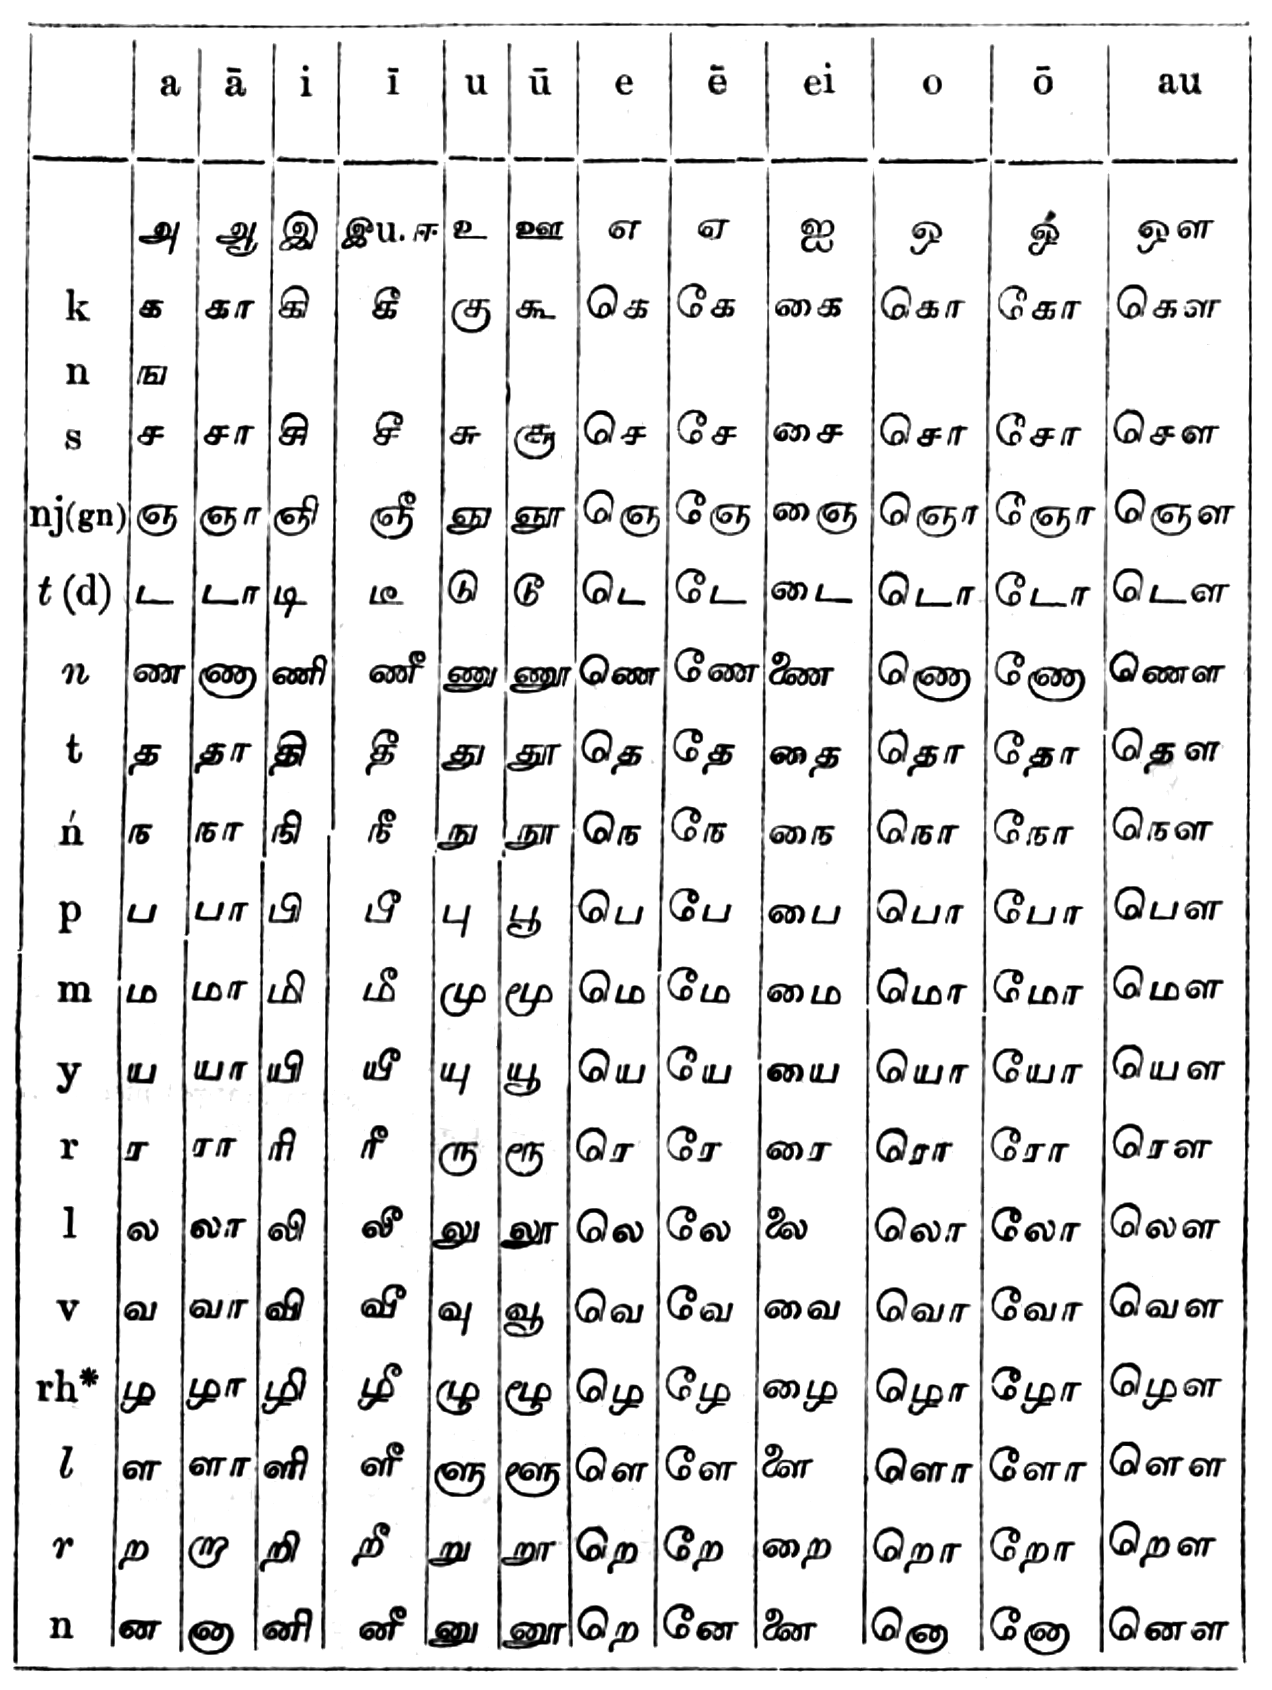
\includegraphics[width=0.9\textwidth,keepaspectratio]{Ziegenbalg-01.png}
\caption*{Tamulische Buchstabirtafel}\footnote{Ein Laut zwischen \emph{r}, \emph{l}. und dem französischen \emph{j}. Jeder nicht mit einem Vokal verbundene oder durch einen Punkt als vokallos bezeichnete Konsonant wird mit kurzem \emph{a} gesprochen.} \footnote{Aus dem Sanskrit entlehnte Buchstaben: \tam{ஸ} s, \tam{ஷ்} sch, \tam{ஐ} j, \tam{க்ஷ} ksch \tam{ஹ} h.}
\end{figure}
\vspace*{\fill}
\clearpage
\end{document}
